% Options for packages loaded elsewhere
\PassOptionsToPackage{unicode}{hyperref}
\PassOptionsToPackage{hyphens}{url}
\PassOptionsToPackage{dvipsnames,svgnames,x11names}{xcolor}
%
\documentclass[
  letterpaper,
  DIV=11,
  numbers=noendperiod]{scrreprt}

\usepackage{amsmath,amssymb}
\usepackage{iftex}
\ifPDFTeX
  \usepackage[T1]{fontenc}
  \usepackage[utf8]{inputenc}
  \usepackage{textcomp} % provide euro and other symbols
\else % if luatex or xetex
  \usepackage{unicode-math}
  \defaultfontfeatures{Scale=MatchLowercase}
  \defaultfontfeatures[\rmfamily]{Ligatures=TeX,Scale=1}
\fi
\usepackage{lmodern}
\ifPDFTeX\else  
    % xetex/luatex font selection
\fi
% Use upquote if available, for straight quotes in verbatim environments
\IfFileExists{upquote.sty}{\usepackage{upquote}}{}
\IfFileExists{microtype.sty}{% use microtype if available
  \usepackage[]{microtype}
  \UseMicrotypeSet[protrusion]{basicmath} % disable protrusion for tt fonts
}{}
\makeatletter
\@ifundefined{KOMAClassName}{% if non-KOMA class
  \IfFileExists{parskip.sty}{%
    \usepackage{parskip}
  }{% else
    \setlength{\parindent}{0pt}
    \setlength{\parskip}{6pt plus 2pt minus 1pt}}
}{% if KOMA class
  \KOMAoptions{parskip=half}}
\makeatother
\usepackage{xcolor}
\setlength{\emergencystretch}{3em} % prevent overfull lines
\setcounter{secnumdepth}{5}
% Make \paragraph and \subparagraph free-standing
\ifx\paragraph\undefined\else
  \let\oldparagraph\paragraph
  \renewcommand{\paragraph}[1]{\oldparagraph{#1}\mbox{}}
\fi
\ifx\subparagraph\undefined\else
  \let\oldsubparagraph\subparagraph
  \renewcommand{\subparagraph}[1]{\oldsubparagraph{#1}\mbox{}}
\fi

\usepackage{color}
\usepackage{fancyvrb}
\newcommand{\VerbBar}{|}
\newcommand{\VERB}{\Verb[commandchars=\\\{\}]}
\DefineVerbatimEnvironment{Highlighting}{Verbatim}{commandchars=\\\{\}}
% Add ',fontsize=\small' for more characters per line
\usepackage{framed}
\definecolor{shadecolor}{RGB}{241,243,245}
\newenvironment{Shaded}{\begin{snugshade}}{\end{snugshade}}
\newcommand{\AlertTok}[1]{\textcolor[rgb]{0.68,0.00,0.00}{#1}}
\newcommand{\AnnotationTok}[1]{\textcolor[rgb]{0.37,0.37,0.37}{#1}}
\newcommand{\AttributeTok}[1]{\textcolor[rgb]{0.40,0.45,0.13}{#1}}
\newcommand{\BaseNTok}[1]{\textcolor[rgb]{0.68,0.00,0.00}{#1}}
\newcommand{\BuiltInTok}[1]{\textcolor[rgb]{0.00,0.23,0.31}{#1}}
\newcommand{\CharTok}[1]{\textcolor[rgb]{0.13,0.47,0.30}{#1}}
\newcommand{\CommentTok}[1]{\textcolor[rgb]{0.37,0.37,0.37}{#1}}
\newcommand{\CommentVarTok}[1]{\textcolor[rgb]{0.37,0.37,0.37}{\textit{#1}}}
\newcommand{\ConstantTok}[1]{\textcolor[rgb]{0.56,0.35,0.01}{#1}}
\newcommand{\ControlFlowTok}[1]{\textcolor[rgb]{0.00,0.23,0.31}{#1}}
\newcommand{\DataTypeTok}[1]{\textcolor[rgb]{0.68,0.00,0.00}{#1}}
\newcommand{\DecValTok}[1]{\textcolor[rgb]{0.68,0.00,0.00}{#1}}
\newcommand{\DocumentationTok}[1]{\textcolor[rgb]{0.37,0.37,0.37}{\textit{#1}}}
\newcommand{\ErrorTok}[1]{\textcolor[rgb]{0.68,0.00,0.00}{#1}}
\newcommand{\ExtensionTok}[1]{\textcolor[rgb]{0.00,0.23,0.31}{#1}}
\newcommand{\FloatTok}[1]{\textcolor[rgb]{0.68,0.00,0.00}{#1}}
\newcommand{\FunctionTok}[1]{\textcolor[rgb]{0.28,0.35,0.67}{#1}}
\newcommand{\ImportTok}[1]{\textcolor[rgb]{0.00,0.46,0.62}{#1}}
\newcommand{\InformationTok}[1]{\textcolor[rgb]{0.37,0.37,0.37}{#1}}
\newcommand{\KeywordTok}[1]{\textcolor[rgb]{0.00,0.23,0.31}{#1}}
\newcommand{\NormalTok}[1]{\textcolor[rgb]{0.00,0.23,0.31}{#1}}
\newcommand{\OperatorTok}[1]{\textcolor[rgb]{0.37,0.37,0.37}{#1}}
\newcommand{\OtherTok}[1]{\textcolor[rgb]{0.00,0.23,0.31}{#1}}
\newcommand{\PreprocessorTok}[1]{\textcolor[rgb]{0.68,0.00,0.00}{#1}}
\newcommand{\RegionMarkerTok}[1]{\textcolor[rgb]{0.00,0.23,0.31}{#1}}
\newcommand{\SpecialCharTok}[1]{\textcolor[rgb]{0.37,0.37,0.37}{#1}}
\newcommand{\SpecialStringTok}[1]{\textcolor[rgb]{0.13,0.47,0.30}{#1}}
\newcommand{\StringTok}[1]{\textcolor[rgb]{0.13,0.47,0.30}{#1}}
\newcommand{\VariableTok}[1]{\textcolor[rgb]{0.07,0.07,0.07}{#1}}
\newcommand{\VerbatimStringTok}[1]{\textcolor[rgb]{0.13,0.47,0.30}{#1}}
\newcommand{\WarningTok}[1]{\textcolor[rgb]{0.37,0.37,0.37}{\textit{#1}}}

\providecommand{\tightlist}{%
  \setlength{\itemsep}{0pt}\setlength{\parskip}{0pt}}\usepackage{longtable,booktabs,array}
\usepackage{calc} % for calculating minipage widths
% Correct order of tables after \paragraph or \subparagraph
\usepackage{etoolbox}
\makeatletter
\patchcmd\longtable{\par}{\if@noskipsec\mbox{}\fi\par}{}{}
\makeatother
% Allow footnotes in longtable head/foot
\IfFileExists{footnotehyper.sty}{\usepackage{footnotehyper}}{\usepackage{footnote}}
\makesavenoteenv{longtable}
\usepackage{graphicx}
\makeatletter
\def\maxwidth{\ifdim\Gin@nat@width>\linewidth\linewidth\else\Gin@nat@width\fi}
\def\maxheight{\ifdim\Gin@nat@height>\textheight\textheight\else\Gin@nat@height\fi}
\makeatother
% Scale images if necessary, so that they will not overflow the page
% margins by default, and it is still possible to overwrite the defaults
% using explicit options in \includegraphics[width, height, ...]{}
\setkeys{Gin}{width=\maxwidth,height=\maxheight,keepaspectratio}
% Set default figure placement to htbp
\makeatletter
\def\fps@figure{htbp}
\makeatother

\KOMAoption{captions}{tableheading}
\makeatletter
\makeatother
\makeatletter
\@ifpackageloaded{bookmark}{}{\usepackage{bookmark}}
\makeatother
\makeatletter
\@ifpackageloaded{caption}{}{\usepackage{caption}}
\AtBeginDocument{%
\ifdefined\contentsname
  \renewcommand*\contentsname{Table of contents}
\else
  \newcommand\contentsname{Table of contents}
\fi
\ifdefined\listfigurename
  \renewcommand*\listfigurename{List of Figures}
\else
  \newcommand\listfigurename{List of Figures}
\fi
\ifdefined\listtablename
  \renewcommand*\listtablename{List of Tables}
\else
  \newcommand\listtablename{List of Tables}
\fi
\ifdefined\figurename
  \renewcommand*\figurename{Figure}
\else
  \newcommand\figurename{Figure}
\fi
\ifdefined\tablename
  \renewcommand*\tablename{Table}
\else
  \newcommand\tablename{Table}
\fi
}
\@ifpackageloaded{float}{}{\usepackage{float}}
\floatstyle{ruled}
\@ifundefined{c@chapter}{\newfloat{codelisting}{h}{lop}}{\newfloat{codelisting}{h}{lop}[chapter]}
\floatname{codelisting}{Listing}
\newcommand*\listoflistings{\listof{codelisting}{List of Listings}}
\makeatother
\makeatletter
\@ifpackageloaded{caption}{}{\usepackage{caption}}
\@ifpackageloaded{subcaption}{}{\usepackage{subcaption}}
\makeatother
\makeatletter
\@ifpackageloaded{tcolorbox}{}{\usepackage[skins,breakable]{tcolorbox}}
\makeatother
\makeatletter
\@ifundefined{shadecolor}{\definecolor{shadecolor}{rgb}{.97, .97, .97}}
\makeatother
\makeatletter
\makeatother
\makeatletter
\makeatother
\ifLuaTeX
  \usepackage{selnolig}  % disable illegal ligatures
\fi
\IfFileExists{bookmark.sty}{\usepackage{bookmark}}{\usepackage{hyperref}}
\IfFileExists{xurl.sty}{\usepackage{xurl}}{} % add URL line breaks if available
\urlstyle{same} % disable monospaced font for URLs
\hypersetup{
  pdftitle={Open Principles of Microeconomics},
  pdfauthor={Justin Johnson},
  colorlinks=true,
  linkcolor={blue},
  filecolor={Maroon},
  citecolor={Blue},
  urlcolor={Blue},
  pdfcreator={LaTeX via pandoc}}

\title{Open Principles of Microeconomics}
\author{Justin Johnson}
\date{2023-10-10}

\begin{document}
\maketitle
\ifdefined\Shaded\renewenvironment{Shaded}{\begin{tcolorbox}[frame hidden, boxrule=0pt, interior hidden, sharp corners, borderline west={3pt}{0pt}{shadecolor}, enhanced, breakable]}{\end{tcolorbox}}\fi

\renewcommand*\contentsname{Table of contents}
{
\hypersetup{linkcolor=}
\setcounter{tocdepth}{2}
\tableofcontents
}
\bookmarksetup{startatroot}

\hypertarget{preface}{%
\chapter*{Preface}\label{preface}}
\addcontentsline{toc}{chapter}{Preface}

\markboth{Preface}{Preface}

\bookmarksetup{startatroot}

\hypertarget{welcome-to-open-principles-of-microeconomics}{%
\chapter*{Welcome to Open Principles of
Microeconomics!}\label{welcome-to-open-principles-of-microeconomics}}
\addcontentsline{toc}{chapter}{Welcome to Open Principles of
Microeconomics!}

\markboth{Welcome to Open Principles of Microeconomics!}{Welcome to Open
Principles of Microeconomics!}

This is a new open textbook, based on the third edition of
OpenStax.org's excellent work. I have made some changes to the text, and
added some new material that draws from my previous years experience
teaching Applied Economics 1101: Principles of Microeconomics at the
University of Minnesota. This is a work in progress and will be finished
by January 2024.

\part{1-Welcome to Economics!}

\hypertarget{chapter-objectives}{%
\chapter{Chapter Objectives}\label{chapter-objectives}}


\includegraphics[width=6.5in,height=2.57in]{media/1-introduction_rId20.jpeg}

Figure 1.1 Do You Use Facebook? Economics is greatly impacted by how
well information travels through society. Today, social media giants
Twitter, Facebook, and Instagram are major forces on the information
super highway. (Credit: modification of "Social Media Mixed Icons -
Banner" by Blogtrepreneur/Flickr, CC BY 2.0)

In this chapter, you will learn about:

\begin{itemize}
\tightlist
\item
  What Is Economics, and Why Is It Important?
\item
  Microeconomics and Macroeconomics
\item
  How Economists Use Theories and Models to Understand Economic Issues
\item
  How Economies Can Be Organized: An Overview of Economic Systems
\end{itemize}

\hypertarget{introduction}{%
\section{Introduction}\label{introduction}}

\hypertarget{bring-it-home}{%
\subsection{Bring It Home}\label{bring-it-home}}

\hypertarget{information-overload-in-the-information-age}{%
\subsubsection{Information Overload in the Information
Age}\label{information-overload-in-the-information-age}}

To post or not to post? Every day we are faced with a myriad of
decisions, from what to have for breakfast, to which show to stream, to
the more complex---``Should I double major and add possibly another
semester of study to my education?'' Our response to these choices
depends on the information we have available at any given moment.
Economists call this ``imperfect'' because we rarely have all the data
we need to make perfect decisions. Despite the lack of perfect
information, we still make hundreds of decisions a day.

Streams, sponsors, and social media are altering the process by which we
make choices, how we spend our time, which movies we see, which products
we buy, and more. Whether they read the reviews or just check the
ratings, it\textquotesingle s unlikely for Americans to make many
significant decisions without these information streams.

As you will see in this course, what happens in economics is affected by
how well and how fast information disseminates through a society, such
as how quickly information travels through Facebook. ``Economists love
nothing better than when deep and liquid markets operate under
conditions of perfect information,'' says Jessica Irvine, National
Economics Editor for News Corp Australia.

This leads us to the topic of this chapter, an introduction to the world
of making decisions, processing information, and understanding behavior
in markets ---the world of economics. Each chapter in this book will
start with a discussion about current (or sometimes past) events and
revisit it at chapter's end---to ``bring home'' the concepts in play.

What is economics and why should you spend your time learning it? After
all, there are other disciplines you could be studying, and other ways
you could be spending your time. As the Bring it Home feature just
mentioned, making choices is at the heart of what economists study, and
your decision to take this course is as much as economic decision as
anything else.

Economics is probably not what you think. It is not primarily about
money or finance. It is not primarily about business. It is not
mathematics. What is it then? It is both a subject area and a way of
viewing the world.

\hypertarget{what-is-economics-and-why-is-it-important}{%
\chapter{1.1 What Is Economics, and Why Is It
Important?}\label{what-is-economics-and-why-is-it-important}}

\hypertarget{learning-objectives}{%
\subsection{Learning Objectives}\label{learning-objectives}}

By the end of this section, you will be able to:

\begin{itemize}
\tightlist
\item
  Discuss the importance of studying economics
\item
  Explain the relationship between production and division of labor
\item
  Evaluate the significance of scarcity
\end{itemize}

Economics is the study of how humans make decisions in the face of
scarcity. These can be individual decisions, family decisions, business
decisions or societal decisions. If you look around carefully, you will
see that scarcity is a fact of life. Scarcity means that human wants for
goods, services and resources exceed what is available. Resources, such
as labor, tools, land, and raw materials are necessary to produce the
goods and services we want but they exist in limited supply. Of course,
the ultimate scarce resource is time- everyone, rich or poor, has just
24 expendable hours in the day to earn income to acquire goods and
services, for leisure time, or for sleep. At any point in time, there is
only a finite amount of resources available.

Think about it this way: In 2015 the labor force in the United States
contained over 158 million workers, according to the U.S. Bureau of
Labor Statistics. The total land area was 3,794,101 square miles. While
these are certainly large numbers, they are not infinite. Because these
resources are limited, so are the numbers of goods and services we
produce with them. Combine this with the fact that human wants seem to
be virtually infinite, and you can see why scarcity is a problem.

\hypertarget{introduction-to-fred}{%
\subsection{Introduction to FRED}\label{introduction-to-fred}}

Data is very important in economics because it describes and measures
the issues and problems that economics seek to understand. A variety of
government agencies publish economic and social data. For this course,
we will generally use data from the St.~Louis Federal Reserve
Bank\textquotesingle s FRED database. FRED is very user friendly. It
allows you to display data in tables or charts, and you can easily
download it into spreadsheet form if you want to use the data for other
purposes. The \href{https://openstax.org/l/FRED/}{FRED website} includes
data on nearly 400,000 domestic and international variables over time,
in the following broad categories:

\begin{itemize}
\tightlist
\item
  Money, Banking \& Finance
\item
  Population, Employment, \& Labor Markets (including Income
  Distribution)
\item
  National Accounts (Gross Domestic Product \& its components), Flow of
  Funds, and International Accounts
\item
  Production \& Business Activity (including Business Cycles)
\item
  Prices \& Inflation (including the Consumer Price Index, the Producer
  Price Index, and the Employment Cost Index)
\item
  International Data from other nations
\item
  U.S. Regional Data
\item
  Academic Data (including Penn World Tables \& NBER Macrohistory
  database)
\end{itemize}

For more information about how to use FRED, see the variety of
\href{https://openstax.org/l/FRED_intro}{videos} on YouTube starting
with this introduction.

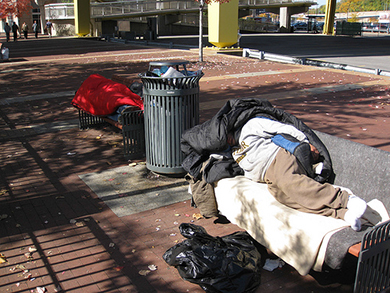
\includegraphics[width=6.5in,height=4.88333in]{media/1-1-what-is-economics-and-why-is-it-important_rId28.jpeg}

Figure 1.2 Scarcity of Resources People experiencing homelessness are a
stark reminder that scarcity of resources is real. (Credit: "Pittsburgh
Homeless" by "daveyinn"/Flickr Creative Commons, CC BY 2.0)

If you still do not believe that scarcity is a problem, consider the
following: Does everyone require food to eat? Does everyone need a
decent place to live? Does everyone have access to healthcare? In every
country in the world, there are people who are hungry, homeless (for
example, those who call park benches their beds, as
\protect\hyperlink{CNX_Econ_C01_003}{Figure 1.2} shows), and in need of
healthcare, just to focus on a few critical goods and services. Why is
this the case? It is because of scarcity. Let's delve into the concept
of scarcity a little deeper, because it is crucial to understanding
economics.

\hypertarget{the-problem-of-scarcity}{%
\subsection{The Problem of Scarcity}\label{the-problem-of-scarcity}}

Think about all the things you consume: food, shelter, clothing,
transportation, healthcare, and entertainment. How do you acquire those
items? You do not produce them yourself. You buy them. How do you afford
the things you buy? You work for pay. If you do not, someone else does
on your behalf. Yet most of us never have enough income to buy all the
things we want. This is because of scarcity. So how do we solve it?

\hypertarget{link-it-up}{%
\subsection{Link It Up}\label{link-it-up}}

Visit this \href{http://openstax.org/l/drought}{website} to read about
how the United States is dealing with scarcity in resources.

Every society, at every level, must make choices about how to use its
resources. Families must decide whether to spend their money on a new
car or a fancy vacation. Towns must choose whether to put more of the
budget into police and fire protection or into the school system.
Nations must decide whether to devote more funds to national defense or
to protecting the environment. In most cases, there just isn't enough
money in the budget to do everything. How do we use our limited
resources the best way possible, that is, to obtain the most goods and
services we can? There are a couple of options. First, we could each
produce everything we each consume. Alternatively, we could each produce
some of what we want to consume, and ``trade'' for the rest of what we
want. Let's explore these options. Why do we not each just produce all
of the things we consume? Think back to pioneer days, when individuals
knew how to do so much more than we do today, from building their homes,
to growing their crops, to hunting for food, to repairing their
equipment. Most of us do not know how to do all---or any---of those
things, but it is not because we could not learn. Rather, we do not have
to. The reason why is something called \emph{the division and
specialization of labor}, a production innovation first put forth by
Adam Smith (\protect\hyperlink{CNX_Econ_C01_008}{Figure 1.3}) in his
book, \emph{The Wealth of Nations}.

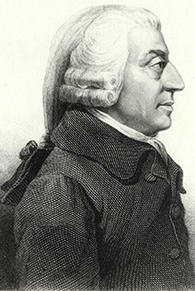
\includegraphics[width=6.5in,height=9.7in]{media/1-1-what-is-economics-and-why-is-it-important_rId34.jpeg}

Figure 1.3 Adam Smith Adam Smith introduced the idea of dividing labor
into discrete tasks. (Credit: "Adam Smith" by Cadell and Davies (1811),
John Horsburgh (1828), or R.C. Bell (1872)/Wikimedia Commons, Public
Domain)

\hypertarget{the-division-of-and-specialization-of-labor}{%
\subsection{The Division of and Specialization of
Labor}\label{the-division-of-and-specialization-of-labor}}

The formal study of economics began when Adam Smith (1723--1790)
published his famous book \emph{The Wealth of Nations} in 1776. Many
authors had written on economics in the centuries before Smith, but he
was the first to address the subject in a comprehensive way. In the
first chapter, Smith introduces the concept of division of labor, which
means that the way one produces a good or service is divided into a
number of tasks that different workers perform, instead of all the tasks
being done by the same person.

To illustrate division of labor, Smith counted how many tasks went into
making a pin: drawing out a piece of wire, cutting it to the right
length, straightening it, putting a head on one end and a point on the
other, and packaging pins for sale, to name just a few. Smith counted 18
distinct tasks that different people performed---all for a pin, believe
it or not!

Modern businesses divide tasks as well. Even a relatively simple
business like a restaurant divides the task of serving meals into a
range of jobs like top chef, sous chefs, less-skilled kitchen help,
servers to wait on the tables, a greeter at the door, janitors to clean
up, and a business manager to handle paychecks and bills---not to
mention the economic connections a restaurant has with suppliers of
food, furniture, kitchen equipment, and the building where it is
located. A complex business like a large manufacturing factory, such as
the shoe factory (\protect\hyperlink{CNX_Econ_C01_009}{Figure 1.4}), or
a hospital can have hundreds of job classifications.

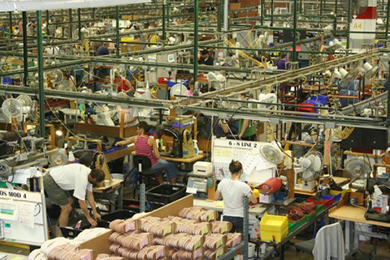
\includegraphics[width=6.5in,height=4.33333in]{media/1-1-what-is-economics-and-why-is-it-important_rId40.jpeg}

Figure 1.4 Division of Labor Workers on an assembly line are an example
of the divisions of labor. (Credit: "Red Wing Shoe Factory Tour" by Nina
Hale/Flickr Creative Commons, CC BY 2.0)

\hypertarget{why-the-division-of-labor-increases-production}{%
\subsection{Why the Division of Labor Increases
Production}\label{why-the-division-of-labor-increases-production}}

When we divide and subdivide the tasks involved with producing a good or
service, workers and businesses can produce a greater quantity of
output. In his observations of pin factories, Smith noticed that one
worker alone might make 20 pins in a day, but that a small business of
10 workers (some of whom would need to complete two or three of the 18
tasks involved with pin-making), could make 48,000 pins in a day. How
can a group of workers, each specializing in certain tasks, produce so
much more than the same number of workers who try to produce the entire
good or service by themselves? Smith offered three reasons.

First, specialization in a particular small job allows workers to focus
on the parts of the production process where they have an advantage. (In
later chapters, we will develop this idea by discussing comparative
advantage.) People have different skills, talents, and interests, so
they will be better at some jobs than at others. The particular
advantages may be based on educational choices, which are in turn shaped
by interests and talents. Only those with medical degrees qualify to
become doctors, for instance. For some goods, geography affects
specialization. For example, it is easier to be a wheat farmer in North
Dakota than in Florida, but easier to run a tourist hotel in Florida
than in North Dakota. If you live in or near a big city, it is easier to
attract enough customers to operate a successful dry cleaning business
or movie theater than if you live in a sparsely populated rural area.
Whatever the reason, if people specialize in the production of what they
do best, they will be more effective than if they produce a combination
of things, some of which they are good at and some of which they are
not.

Second, workers who specialize in certain tasks often learn to produce
more quickly and with higher quality. This pattern holds true for many
workers, including assembly line laborers who build cars, stylists who
cut hair, and doctors who perform heart surgery. In fact, specialized
workers often know their jobs well enough to suggest innovative ways to
do their work faster and better.

A similar pattern often operates within businesses. In many cases, a
business that focuses on one or a few products (sometimes called its
``core competency'') is more successful than firms that try to make a
wide range of products.

Third, specialization allows businesses to take advantage of economies
of scale, which means that for many goods, as the level of production
increases, the average cost of producing each individual unit declines.
For example, if a factory produces only 100 cars per year, each car will
be quite expensive to make on average. However, if a factory produces
50,000 cars each year, then it can set up an assembly line with huge
machines and workers performing specialized tasks, and the average cost
of production per car will be lower. The ultimate result of workers who
can focus on their preferences and talents, learn to do their
specialized jobs better, and work in larger organizations is that
society as a whole can produce and consume far more than if each person
tried to produce all of their own goods and services. The division and
specialization of labor has been a force against the problem of
scarcity.

\hypertarget{trade-and-markets}{%
\subsection{Trade and Markets}\label{trade-and-markets}}

Specialization only makes sense, though, if workers can use the pay they
receive for doing their jobs to purchase the other goods and services
that they need. In short, specialization requires trade.

You do not have to know anything about electronics or sound systems to
play music---you just buy an iPod or MP3 player, download the music, and
listen. You do not have to know anything about artificial fibers or the
construction of sewing machines if you need a jacket---you just buy the
jacket and wear it. You do not need to know anything about internal
combustion engines to operate a car---you just get in and drive. Instead
of trying to acquire all the knowledge and skills involved in producing
all of the goods and services that you wish to consume, the market
allows you to learn a specialized set of skills and then use the pay you
receive to buy the goods and services you need or want. This is how our
modern society has evolved into a strong economy.

\hypertarget{why-study-economics}{%
\subsection{Why Study Economics?}\label{why-study-economics}}


\includegraphics[width=6.34in,height=2.63in]{media/1-1-what-is-economics-and-why-is-it-important_rId53.jpeg}

Figure 1.5 Esther Duflo, Abhijit Banerjee, and Michael Kremer Esther
Duflo, Abhijit Banerjee (both from Massachusetts Institute of
Technology), and Michael Kremer (University of Chicago) were awarded the
Nobel Prize for groundbreaking work in which they established
experimental methods to understand poverty and outcomes of initiatives
to address it. (Credit: modification of work by U.S. Embassy
Sweden/Wikimedia Commons, CC BY 2.0; Financial Times/Wikimedia Commons,
CC BY 2.0; U.S. Embassy Sweden/Flickr Creative Commons, CC BY 2.0)

Now that you have an overview on what economics studies, let's quickly
discuss why you are right to study it. Economics is not primarily a
collection of facts to memorize, although there are plenty of important
concepts to learn. Instead, think of economics as a collection of
questions to answer or puzzles to work. Most importantly, economics
provides the tools to solve those puzzles.

Consider the complex and critical issue of education barriers on
national and regional levels, which affect millions of people and result
in widespread poverty and inequality. Governments, aid organizations,
and wealthy individuals spend billions of dollars each year trying to
address these issues. Nations announce the revitalization of their
education programs; tech companies donate devices and infrastructure,
and celebrities and charities build schools and sponsor students. Yet
the problems remain, sometimes almost as pronounced as they were before
the intervention. Why is that the case? In 2019, three
economists---Esther Duflo, Abhijit Banerjee, and Michael Kremer---were
awarded the Nobel Prize for their work to answer those questions. They
worked diligently to break the widespread problems into smaller pieces,
and experimented with small interventions to test success. The award
citation credited their work with giving the world better tools and
information to address poverty and improve education. Esther Duflo, who
is the youngest person and second woman to win the Nobel Prize in
Economics, said, "We believed that like the war on cancer, the war on
poverty was not going to be won in one major battle, but in a series of
small triumphs. . . . This work and the culture of learning that it
fostered in governments has led to real improvement in the lives of
hundreds of millions of poor people.''

As you can see, economics affects far more than business. For example:

\begin{itemize}
\tightlist
\item
  Virtually every major problem facing the world today, from global
  warming, to world poverty, to the conflicts in Syria, Afghanistan, and
  Somalia, has an economic dimension. If you are going to be part of
  solving those problems, you need to be able to understand them.
  Economics is crucial.
\item
  It is hard to overstate the importance of economics to good
  citizenship. You need to be able to vote intelligently on budgets,
  regulations, and laws in general. When the U.S. government came close
  to a standstill at the end of 2012 due to the ``fiscal cliff,'' what
  were the issues? Did you know?
\item
  A basic understanding of economics makes you a well-rounded thinker.
  When you read articles about economic issues, you will understand and
  be able to evaluate the writer's argument. When you hear classmates,
  co-workers, or political candidates talking about economics, you will
  be able to distinguish between common sense and nonsense. You will
  find new ways of thinking about current events and about personal and
  business decisions, as well as current events and politics.
\end{itemize}

The study of economics does not dictate the answers, but it can
illuminate the different choices.

\hypertarget{microeconomics-and-macroeconomics}{%
\chapter{1.2 Microeconomics and
Macroeconomics}\label{microeconomics-and-macroeconomics}}

\hypertarget{learning-objectives-1}{%
\subsection{Learning Objectives}\label{learning-objectives-1}}

By the end of this section, you will be able to:

\begin{itemize}
\tightlist
\item
  Describe microeconomics
\item
  Describe macroeconomics
\item
  Contrast monetary policy and fiscal policy
\end{itemize}

Economics is concerned with the well-being of \emph{all} people,
including those with jobs and those without jobs, as well as those with
high incomes and those with low incomes. Economics acknowledges that
production of useful goods and services can create problems of
environmental pollution. It explores the question of how investing in
education helps to develop workers' skills. It probes questions like how
to tell when big businesses or big labor unions are operating in a way
that benefits society as a whole and when they are operating in a way
that benefits their owners or members at the expense of others. It looks
at how government spending, taxes, and regulations affect decisions
about production and consumption.

It should be clear by now that economics covers considerable ground. We
can divide that ground into two parts: Microeconomics focuses on the
actions of individual agents within the economy, like households,
workers, and businesses. Macroeconomics looks at the economy as a whole.
It focuses on broad issues such as growth of production, the number of
unemployed people, the inflationary increase in prices, government
deficits, and levels of exports and imports. Microeconomics and
macroeconomics are not separate subjects, but rather complementary
perspectives on the overall subject of the economy.

To understand why both microeconomic and macroeconomic perspectives are
useful, consider the problem of studying a biological ecosystem like a
lake. One person who sets out to study the lake might focus on specific
topics: certain kinds of algae or plant life; the characteristics of
particular fish or snails; or the trees surrounding the lake. Another
person might take an overall view and instead consider the
lake\textquotesingle s ecosystem from top to bottom; what eats what, how
the system stays in a rough balance, and what environmental stresses
affect this balance. Both approaches are useful, and both examine the
same lake, but the viewpoints are different. In a similar way, both
microeconomics and macroeconomics study the same economy, but each has a
different viewpoint.

Whether you are scrutinizing lakes or economics, the micro and the macro
insights should blend with each other. In studying a lake, the micro
insights about particular plants and animals help to understand the
overall food chain, while the macro insights about the overall food
chain help to explain the environment in which individual plants and
animals live.

In economics, the micro decisions of individual businesses are
influenced by whether the macroeconomy is healthy. For example, firms
will be more likely to hire workers if the overall economy is growing.
In turn, macroeconomy\textquotesingle s performance ultimately depends
on the microeconomic decisions that individual households and businesses
make.

\hypertarget{microeconomics}{%
\subsection{Microeconomics}\label{microeconomics}}

What determines how households and individuals spend their budgets? What
combination of goods and services will best fit their needs and wants,
given the budget they have to spend? How do people decide whether to
work, and if so, whether to work full time or part time? How do people
decide how much to save for the future, or whether they should borrow to
spend beyond their current means?

What determines the products, and how many of each, a firm will produce
and sell? What determines the prices a firm will charge? What determines
how a firm will produce its products? What determines how many workers
it will hire? How will a firm finance its business? When will a firm
decide to expand, downsize, or even close? In the microeconomics part of
this book, we will learn about the theory of consumer behavior, the
theory of the firm, how markets for labor and other resources work, and
how markets sometimes fail to work properly.

\hypertarget{macroeconomics}{%
\subsection{Macroeconomics}\label{macroeconomics}}

What determines the level of economic activity in a society? In other
words, what determines how many goods and services a nation actually
produces? What determines how many jobs are available in an economy?
What determines a nation's standard of living? What causes the economy
to speed up or slow down? What causes firms to hire more workers or to
lay them off? Finally, what causes the economy to grow over the long
term?

We can determine an economy\textquotesingle s macroeconomic health by
examining a number of goals: growth in the standard of living, low
unemployment, and low inflation, to name the most important. How can we
use government macroeconomic policy to pursue these goals? A
nation\textquotesingle s central bank conducts monetary policy, which
involves policies that affect bank lending, interest rates, and
financial capital markets. For the United States, this is the Federal
Reserve. A nation\textquotesingle s legislative body determines fiscal
policy, which involves government spending and taxes. For the United
States, this is the Congress and the executive branch, which originates
the federal budget. These are the government\textquotesingle s main
tools. Americans tend to expect that government can fix whatever
economic problems we encounter, but to what extent is that expectation
realistic? These are just some of the issues that we will explore in the
macroeconomic chapters of this book.

\hypertarget{how-economists-use-theories-and-models-to-understand-economic-issues}{%
\chapter{1.3 How Economists Use Theories and Models to Understand
Economic
Issues}\label{how-economists-use-theories-and-models-to-understand-economic-issues}}

\hypertarget{learning-objectives-2}{%
\subsection{Learning Objectives}\label{learning-objectives-2}}

By the end of this section, you will be able to:

\begin{itemize}
\tightlist
\item
  Interpret a circular flow diagram
\item
  Explain the importance of economic theories and models
\item
  Describe goods and services markets and labor markets
\end{itemize}

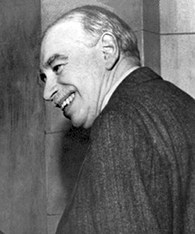
\includegraphics[width=6.5in,height=7.8in]{media/1-3-how-economists-use-theories-and-models-to-understand-economic-issues_rId22.jpeg}

Figure 1.6 John Maynard Keynes One of the most influential economists in
modern times was John Maynard Keynes. (Credit: ``John Maynard Keynes''
by IMF/Wikimedia Commons, Public Domain)

John Maynard Keynes (1883--1946), one of the greatest economists of the
twentieth century, pointed out that economics is not just a subject area
but also a way of thinking. Keynes
(\protect\hyperlink{CNX_Econ_C01_004}{Figure 1.6}) famously wrote in the
introduction to a fellow economist's book: ``{[}Economics{]} is a method
rather than a doctrine, an apparatus of the mind, a technique of
thinking, which helps its possessor to draw correct conclusions.'' In
other words, economics teaches you how to think, not what to think.

\hypertarget{link-it-up}{%
\subsection{Link It Up}\label{link-it-up}}

Watch this \href{http://openstax.org/l/Keynes}{video} about John Maynard
Keynes and his influence on economics.

Economists see the world through a different lens than anthropologists,
biologists, classicists, or practitioners of any other discipline. They
analyze issues and problems using economic theories that are based on
particular assumptions about human behavior. These assumptions tend to
be different than the assumptions an anthropologist or psychologist
might use. A theory is a simplified representation of how two or more
variables interact with each other. The purpose of a theory is to take a
complex, real-world issue and simplify it down to its essentials. If
done well, this enables the analyst to understand the issue and any
problems around it. A good theory is simple enough to understand, while
complex enough to capture the key features of the object or situation
you are studying.

Sometimes economists use the term model instead of theory. Strictly
speaking, a theory is a more abstract representation, while a model is a
more applied or empirical representation. We use models to test
theories, but for this course we will use the terms interchangeably.

For example, an architect who is planning a major office building will
often build a physical model that sits on a tabletop to show how the
entire city block will look after the new building is constructed.
Companies often build models of their new products, which are more rough
and unfinished than the final product, but can still demonstrate how the
new product will work.

A good model to start with in economics is the circular flow diagram
(\protect\hyperlink{CNX_Econ_C01_002}{Figure 1.7}). It pictures the
economy as consisting of two groups---households and firms---that
interact in two markets: the goods and services market in which firms
sell and households buy and the labor market in which households sell
labor to business firms or other employees.

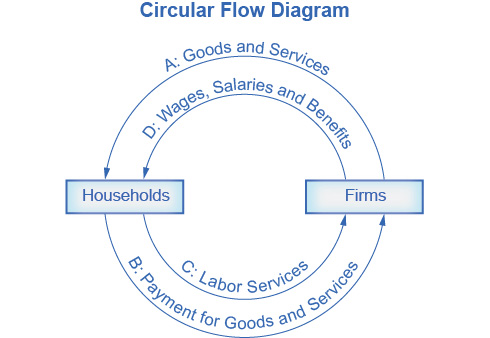
\includegraphics[width=3.26667in,height=2.25333in]{media/1-3-how-economists-use-theories-and-models-to-understand-economic-issues_rId33.jpeg}

Figure 1.7 The Circular Flow Diagram The circular flow diagram shows how
households and firms interact in the goods and services market, and in
the labor market. The direction of the arrows shows that in the goods
and services market, households receive goods and services and pay firms
for them. In the labor market, households provide labor and receive
payment from firms through wages, salaries, and benefits.

Firms produce and sell goods and services to households in the market
for goods and services (or product market). Arrow ``A'' indicates this.
Households pay for goods and services, which becomes the revenues to
firms. Arrow ``B'' indicates this. Arrows A and B represent the two
sides of the product market. Where do households obtain the income to
buy goods and services? They provide the labor and other resources
(e.g., land, capital, raw materials) firms need to produce goods and
services in the market for inputs (or factors of production). Arrow
``C'' indicates this. In return, firms pay for the inputs (or resources)
they use in the form of wages and other factor payments. Arrow ``D''
indicates this. Arrows ``C'' and ``D'' represent the two sides of the
factor market.

Of course, in the real world, there are many different markets for goods
and services and markets for many different types of labor. The circular
flow diagram simplifies this to make the picture easier to grasp. In the
diagram, firms produce goods and services, which they sell to households
in return for revenues. The outer circle shows this, and represents the
two sides of the product market (for example, the market for goods and
services) in which households demand and firms supply. Households sell
their labor as workers to firms in return for wages, salaries, and
benefits. The inner circle shows this and represents the two sides of
the labor market in which households supply and firms demand.

This version of the circular flow model is stripped down to the
essentials, but it has enough features to explain how the product and
labor markets work in the economy. We could easily add details to this
basic model if we wanted to introduce more real-world elements, like
financial markets, governments, and interactions with the rest of the
globe (imports and exports).

Economists carry a set of theories in their heads like a carpenter
carries around a toolkit. When they see an economic issue or problem,
they go through the theories they know to see if they can find one that
fits. Then they use the theory to derive insights about the issue or
problem. Economists express theories as diagrams, graphs, or even as
mathematical equations. (Do not worry. In this course, we will mostly
use graphs.) Economists do not figure out the answer to the problem
first and then draw the graph to illustrate. Rather, they use the graph
of the theory to help them figure out the answer. Although at the
introductory level, you can sometimes figure out the right answer
without applying a model, if you keep studying economics, before too
long you will run into issues and problems that you will need to graph
to solve. We explain both micro and macroeconomics in terms of theories
and models. The most well-known theories are probably those of supply
and demand, but you will learn a number of others.

\hypertarget{how-to-organize-economies-an-overview-of-economic-systems}{%
\chapter{1.4 How To Organize Economies: An Overview of Economic
Systems}\label{how-to-organize-economies-an-overview-of-economic-systems}}

\hypertarget{learning-objectives-3}{%
\subsection{Learning Objectives}\label{learning-objectives-3}}

By the end of this section, you will be able to:

\begin{itemize}
\tightlist
\item
  Contrast traditional economies, command economies, and market
  economies
\item
  Explain gross domestic product (GDP)
\item
  Assess the importance and effects of globalization
\end{itemize}

Think about what a complex system a modern economy is. It includes all
production of goods and services, all buying and selling, all
employment. The economic life of every individual is interrelated, at
least to a small extent, with the economic lives of thousands or even
millions of other individuals. Who organizes and coordinates this
system? Who ensures that, for example, the number of televisions a
society provides is the same as the amount it needs and wants? Who
ensures that the right number of employees work in the electronics
industry? Who ensures that televisions are produced in the best way
possible? How does it all get done?

There are at least three ways that societies organize an economy. The
first is the traditional economy, which is the oldest economic system
and is used in parts of Asia, Africa, and South America. Traditional
economies organize their economic affairs the way they have always done
(i.e., tradition). Occupations stay in the family. Most families are
farmers who grow the crops using traditional methods. What you produce
is what you consume. Because tradition drives the way of life, there is
little economic progress or development.

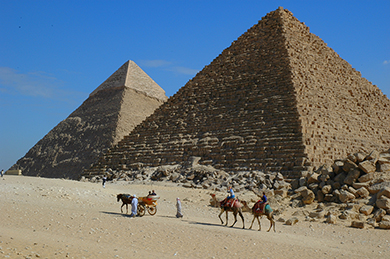
\includegraphics[width=6.5in,height=4.31667in]{media/1-4-how-to-organize-economies-an-overview-of-economic-systems_rId23.jpeg}

Figure 1.8 A Command Economy Ancient Egypt was an example of a command
economy. (Credit: "Pyramids at Giza" by Jay Bergesen/Flickr Creative
Commons, CC BY 2.0)

Command economies are very different. In a command economy, economic
effort is devoted to goals passed down from a ruler or ruling class.
Ancient Egypt was a good example: a large part of economic life was
devoted to building pyramids, like those in
\protect\hyperlink{CNX_Econ_C01_005}{Figure 1.8}, for the pharaohs.
Medieval manor life is another example: the lord provided the land for
growing crops and protection in the event of war. In return, vassals
provided labor and soldiers to do the lord's bidding. In the last
century, communism emphasized command economies.

In a command economy, the government decides what goods and services
will be produced and what prices it will charge for them. The government
decides what methods of production to use and sets wages for workers.
The government provides many necessities like healthcare and education
for free. Currently, Cuba and North Korea have command economies.


\includegraphics[width=6.5in,height=6.53333in]{media/1-4-how-to-organize-economies-an-overview-of-economic-systems_rId27.jpeg}

Figure 1.9 A Market Economy Nothing says ``market'' more than The New
York Stock Exchange. (Credit: work by Erik Drost/Flickr Creative
Commons, CC BY 2.0)

Although command economies have a very centralized structure for
economic decisions, market economies have a very decentralized
structure. A market is an institution that brings together buyers and
sellers of goods or services, who may be either individuals or
businesses. The New York Stock Exchange
(\protect\hyperlink{CNX_Econ_C01_006}{Figure 1.9}) is a prime example of
a market which brings buyers and sellers together. In a market economy,
decision-making is decentralized. Market economies are based on private
enterprise: the private individuals or groups of private individuals own
and operate the means of production (resources and businesses).
Businesses supply goods and services based on demand. (In a command
economy, by contrast, the government owns resources and businesses.)
Supply of goods and services depends on what the demands are. A person's
income is based on their ability to convert resources (especially labor)
into something that society values. The more society values the person's
output, the higher the income (think Lady Gaga or LeBron James). In this
scenario, market forces, not governments, determine economic decisions.

Most economies in the real world are mixed. They combine elements of
command and market (and even traditional) systems. The U.S. economy is
positioned toward the market-oriented end of the spectrum. Many
countries in Europe and Latin America, while primarily market-oriented,
have a greater degree of government involvement in economic decisions
than the U.S. economy. China and Russia, while over the past several
decades have moved more in the direction of having a market-oriented
system, remain closer to the command economy end of the spectrum. The
Heritage Foundation provides perspective on countries' economic freedom,
as the following Clear It Up feature discusses.

\hypertarget{clear-it-up}{%
\subsection{Clear It Up}\label{clear-it-up}}

\hypertarget{what-countries-are-considered-economically-free}{%
\subsubsection{What countries are considered economically
free?}\label{what-countries-are-considered-economically-free}}

Who is in control of economic decisions? Are people free to do what they
want and to work where they want? Are businesses free to produce when
they want and what they choose, and to hire and fire as they wish? Are
banks free to choose who will receive loans, or does the government
control these kinds of choices? Each year, researchers at the Heritage
Foundation and the \emph{Wall Street Journal} look at 50 different
categories of economic freedom for countries around the world. They give
each nation a score based on the extent of economic freedom in each
category. Note that while the Heritage Foundation/WSJ index is widely
cited by an array of scholars and publications, it should be regarded as
only one viewpoint. Some experts indicate that the index's category
choices and scores are politically biased. However, the index and others
like it provide a useful resource for critical discussion of economic
freedom.

The 2016 Heritage Foundation's Index of Economic Freedom report ranked
178 countries around the world: \protect\hyperlink{Table_01_01}{Table
1.1} lists some examples of the most free and the least free countries.
Although technically not a separate country, Hong Kong has been granted
a degree of autonomy such that, for purposes of measuring economic
statistics, it is often treated as a separate country. Several
additional countries were not ranked because of extreme instability that
made judgments about economic freedom impossible. These countries
include Afghanistan, Iraq, Libya, Syria, Somalia, and Yemen.

The assigned rankings are inevitably based on estimates, yet even these
rough measures can be useful for discerning trends. In 2015, 101 of the
178 included countries shifted toward greater economic freedom, although
77 of the countries shifted toward less economic freedom. In recent
decades, the overall trend has been a \emph{higher level of economic
freedom around the world}.

Table 1.1 Economic Freedoms, 2016 (Source: The Heritage Foundation, 2016
Index of Economic Freedom, Country Rankings,
http://www.heritage.org/index/ranking)

\hypertarget{regulations-the-rules-of-the-game}{%
\subsection{Regulations: The Rules of the
Game}\label{regulations-the-rules-of-the-game}}

Markets and government regulations are always entangled. There is no
such thing as an absolutely free market. Regulations always define the
``rules of the game'' in the economy. Economies that are primarily
market-oriented have fewer regulations---ideally just enough to maintain
an even playing field for participants. At a minimum, these laws govern
matters like safeguarding private property against theft, protecting
people from violence, enforcing legal contracts, preventing fraud, and
collecting taxes. Conversely, even the most command-oriented economies
operate using markets. How else would buying and selling occur? The
government heavily regulates decisions of what to produce and prices to
charge. Heavily regulated economies often have underground economies (or
black markets), which are markets where the buyers and sellers make
transactions without the government's approval.

The question of how to organize economic institutions is typically not a
straightforward choice between all market or all government, but instead
involves a balancing act over the appropriate combination of market
freedom and government rules.

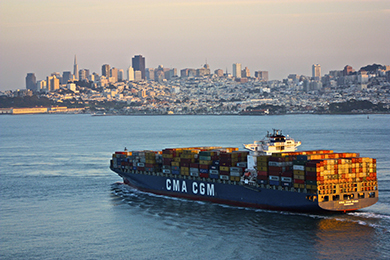
\includegraphics[width=6.5in,height=4.33333in]{media/1-4-how-to-organize-economies-an-overview-of-economic-systems_rId35.jpeg}

Figure 1.10 Globalization Cargo ships are one mode of transportation for
shipping goods in the global economy. (Credit: "Cargo Ship" by Raul
Valdez/Flickr Creative Commons, CC BY 2.0)

\hypertarget{the-rise-of-globalization}{%
\subsection{The Rise of Globalization}\label{the-rise-of-globalization}}

Recent decades have seen a trend toward globalization, which is the
expanding cultural, political, and economic connections between people
around the world. One measure of this is the increased buying and
selling of goods, services, and assets across national borders---in
other words, international trade and financial capital flows.

Globalization has occurred for a number of reasons. Improvements in
shipping, as illustrated by the container ship in
\protect\hyperlink{CNX_Econ_C01_007}{Figure 1.10}, and air cargo have
driven down transportation costs. Innovations in computing and
telecommunications have made it easier and cheaper to manage
long-distance economic connections of production and sales. Many
valuable products and services in the modern economy can take the form
of information---for example: computer software; financial advice;
travel planning; music, books and movies; and blueprints for designing a
building. These products and many others can be transported over
telephones and computer networks at ever-lower costs. Finally,
international agreements and treaties between countries have encouraged
greater trade.

\protect\hyperlink{Table_01_02}{Table 1.2} presents one measure of
globalization. It shows the percentage of domestic economic production
that was exported for a selection of countries from 2010 to 2015,
according to an entity known as The World Bank. Exports are the goods
and services that one produces domestically and sells abroad. Imports
are the goods and services that one produces abroad and then sells
domestically. Gross domestic product (GDP) measures the size of total
production in an economy. Thus, the ratio of exports divided by GDP
measures what share of a country's total economic production is sold in
other countries.

Table 1.2 The Extent of Globalization (exports/GDP) (Source:
http://databank.worldbank.org/data/)

In recent decades, the export/GDP ratio has generally risen, both
worldwide and for the U.S. economy. Interestingly, the share of U.S.
exports in proportion to the U.S. economy is well below the global
average, in part because large economies like the United States can
contain more of the division of labor inside their national borders.
However, smaller economies like Belgium, Korea, and Canada need to trade
across their borders with other countries to take full advantage of
division of labor, specialization, and economies of scale. In this
sense, the enormous U.S. economy is less affected by globalization than
most other countries.

\protect\hyperlink{Table_01_02}{Table 1.2} indicates that many medium
and low income countries around the world, like Mexico and China, have
also experienced a surge of globalization in recent decades. If an
astronaut in orbit could put on special glasses that make all economic
transactions visible as brightly colored lines and look down at Earth,
the astronaut would see the planet covered with connections.

Despite the rise in globalization over the last few decades, in recent
years we\textquotesingle ve seen significant pushback against
globalization from people across the world concerned about loss of jobs,
loss of political sovereignty, and increased economic inequality.
Prominent examples of this pushback include the 2016 vote in Great
Britain to exit the European Union (i.e.~Brexit), and the election of
Donald J. Trump for President of the United States.

Hopefully, you now have an idea about economics. Before you move to any
other chapter of study, be sure to read the very important appendix to
this chapter called
\href{http://openstax.org/books/principles-microeconomics-3e/pages/a-the-use-of-mathematics-in-principles-of-economics}{The
Use of Mathematics in Principles of Economics}. It is essential that you
learn more about how to read and use models in economics.

\hypertarget{bring-it-home}{%
\subsection{Bring It Home}\label{bring-it-home}}

\hypertarget{information-overload-in-the-information-age}{%
\subsubsection{Information Overload in the Information
Age}\label{information-overload-in-the-information-age}}

The world provides nearly instant access to a wealth of information.
Consider that as recently as the late 1970s, the \emph{Farmer's
Almanac}, along with the Weather Bureau of the U.S. Department of
Agriculture, were the primary sources American farmers used to determine
when to plant and harvest their crops. Today, these decisions are driven
by data. Farmers access detailed data streams driven by global
positioning systems, historical rainfall patterns, and complex weather
monitoring services. They combine this information with crop yield data
and soil quality measurements from prior years. Maximizing production
efficiently can mean the difference between a farm that remains
profitable and one that may need to sell its land, and data helps
eliminate guesswork.

Information helps us make decisions as simple as what to wear today to
how many reporters the media should send to cover an event. Each of
these decisions is an economic decision. After all, resources are
scarce. If the media send ten reporters to cover an announcement, they
are not available to cover other stories or complete other tasks.
Information provides the necessary knowledge to make the best possible
decisions on how to utilize scarce resources. Welcome to the world of
economics!

\part{2-Choice in a World of Scarcity}

\hypertarget{chapter-objectives}{%
\chapter{Chapter Objectives}\label{chapter-objectives}}


\includegraphics[width=6.34in,height=4.86in]{media/2-introduction-to-choice-in-a-world-of-scarcity_rId20.jpeg}

Figure 2.1 Choices and Tradeoffs In general, the higher the degree, the
higher the salary, so why aren't more people pursuing higher degrees?
The short answer: choices and tradeoffs. (Credit: modification of
"College of DuPage Commencement 2018 107" by COD Newsroom/Flickr, CC BY
2.0)

In this chapter, you will learn about:

\begin{itemize}
\tightlist
\item
  How Individuals Make Choices Based on Their Budget Constraint
\item
  The Production Possibilities Frontier and Social Choices
\item
  Confronting Objections to the Economic Approach
\end{itemize}

\hypertarget{introduction-to-choice-in-a-world-of-scarcity}{%
\section{Introduction to Choice in a World of
Scarcity}\label{introduction-to-choice-in-a-world-of-scarcity}}

\hypertarget{bring-it-home}{%
\subsection{Bring It Home}\label{bring-it-home}}

\hypertarget{choices-...-to-what-degree}{%
\subsubsection{Choices ... to What
Degree?}\label{choices-...-to-what-degree}}

Does your level of education impact earning? Let's look at some data
from the Bureau of Labor Statistics (BLS). In 2020, among full-time wage
and salary workers, median weekly earnings for those with a master's
degree were \$1,545. Multiply this average by 52 weeks, and you get
average annual earnings of \$80,340. Compare that to the median weekly
earnings for full-time workers aged 25 and over with just a bachelor's
degree: \$1,305 weekly and \$67,860 a year. What about those with no
higher than a high school diploma in 2020? They earn an average of just
\$781 weekly and \$40,612 over 12 months. In other words, data from the
BLS indicates that receiving a bachelor's degree boosts earnings by 67\%
over what workers would have earned if they only obtained a high school
diploma, and a master's degree yields average earnings that are nearly
double those of workers with a high school diploma.

Given these statistics, we might expect many people to choose to go to
college and at least earn a bachelor's degree. Assuming that people want
to improve their material well-being, it seems like they would make
those choices that provide them with the greatest opportunity to consume
goods and services. As it turns out, the analysis is not nearly as
simple as this. In fact, in 2019, the BLS reported that while just over
90\% of the population aged 25 and over in the United States had a high
school diploma, only 36\% of those aged 25 and over had a
bachelor\textquotesingle s or higher degree, and only 13.5\% had earned
a master\textquotesingle s or higher degree.

This brings us to the subject of this chapter: why people make the
choices they make and how economists explain those choices.

You will learn quickly when you examine the relationship between
economics and scarcity that choices involve tradeoffs. Every choice has
a cost.

In 1968, the Rolling Stones recorded ``You Can't Always Get What You
Want.'' Economists chuckled, because they had been singing a similar
tune for decades. English economist Lionel Robbins (1898--1984), in his
\emph{Essay on the Nature and Significance of Economic Science} in 1932,
described not always getting what you want in this way:

\begin{quote}
The time at our disposal is limited. There are only twenty-four hours in
the day. We have to choose between the different uses to which they may
be put. ... Everywhere we turn, if we choose one thing we must
relinquish others which, in different circumstances, we would wish not
to have relinquished. Scarcity of means to satisfy given ends is an
almost ubiquitous condition of human nature.
\end{quote}

Because people live in a world of scarcity, they cannot have all the
time, money, possessions, and experiences they wish. Neither can
society.

This chapter will continue our discussion of scarcity and the economic
way of thinking by first introducing three critical concepts:
opportunity cost, marginal decision making, and diminishing returns.
Later, it will consider whether the economic way of thinking accurately
describes either how we \emph{make} choices and how we \emph{should}
make them.

\hypertarget{how-individuals-make-choices-based-on-their-budget-constraint}{%
\chapter{2.1 How Individuals Make Choices Based on Their Budget
Constraint}\label{how-individuals-make-choices-based-on-their-budget-constraint}}

\hypertarget{learning-objectives-4}{%
\subsection{Learning Objectives}\label{learning-objectives-4}}

By the end of this section, you will be able to:

\begin{itemize}
\tightlist
\item
  Calculate and graph budget constraints
\item
  Explain opportunity sets and opportunity costs
\item
  Evaluate the law of diminishing marginal utility
\item
  Explain how marginal analysis and utility influence choices
\end{itemize}

Consider the typical consumer's budget problem. Consumers have a limited
amount of income to spend on the things they need and want. Suppose
Alphonso has \$10 in spending money each week that he can allocate
between bus tickets for getting to work and the burgers that he eats for
lunch. Burgers cost \$2 each, and bus tickets are 50 cents each. We can
see Alphonso\textquotesingle s budget problem in
\protect\hyperlink{CNX_Econ_C02_001}{Figure 2.2}.

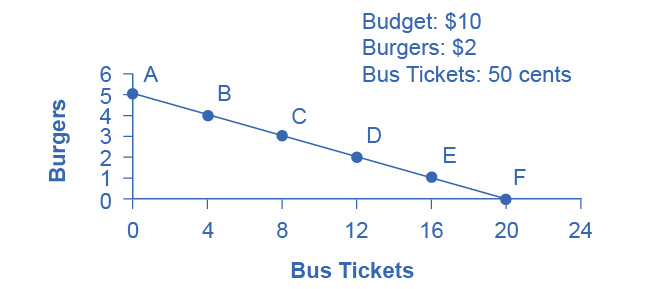
\includegraphics[width=3.25in,height=1.445in]{media/2-1-how-individuals-make-choices-based-on-their-budget-constraint_rId22.jpeg}

Figure 2.2 The Budget Constraint: Alphonso's Consumption Choice
Opportunity Frontier Each point on the budget constraint represents a
combination of burgers and bus tickets whose total cost adds up to
Alphonso's budget of \$10. The relative price of burgers and bus tickets
determines the slope of the budget constraint. All along the budget set,
giving up one burger means gaining four bus tickets.

The vertical axis in the figure shows burger purchases and the
horizontal axis shows bus ticket purchases. If Alphonso spends all his
money on burgers, he can afford five per week. (\$10 per week/\$2 per
burger = 5 burgers per week.) However, if he does this, he will not be
able to afford any bus tickets. Point A in the figure shows the choice
(zero bus tickets and five burgers). Alternatively, if Alphonso spends
all his money on bus tickets, he can afford 20 per week. (\$10 per
week/\$0.50 per bus ticket = 20 bus tickets per week.) Then, however, he
will not be able to afford any burgers. Point F shows this alternative
choice (20 bus tickets and zero burgers).

If we connect all the points between A and F, we get
Alphonso\textquotesingle s budget constraint. This indicates all the
combination of burgers and bus tickets Alphonso can afford, given the
price of the two goods and his budget amount.

If Alphonso is like most people, he will choose some combination that
includes both bus tickets and burgers. That is, he will choose some
combination on the budget constraint that is between points A and F.
Every point on (or inside) the constraint shows a combination of burgers
and bus tickets that Alphonso can afford. Any point outside the
constraint is not affordable, because it would cost more money than
Alphonso has in his budget.

The budget constraint clearly shows the tradeoff Alphonso faces in
choosing between burgers and bus tickets. Suppose he is currently at
point D, where he can afford 12 bus tickets and two burgers. What would
it cost Alphonso for one more burger? It would be natural to answer \$2,
but that's not the way economists think. Instead they ask, how many bus
tickets would Alphonso have to give up to get one more burger, while
staying within his budget? Since bus tickets cost 50 cents, Alphonso
would have to give up four to afford one more burger. That is the true
cost to Alphonso.

\hypertarget{the-concept-of-opportunity-cost}{%
\subsection{The Concept of Opportunity
Cost}\label{the-concept-of-opportunity-cost}}

Economists use the term opportunity cost to indicate what people must
give up to obtain what they desire. The idea behind opportunity cost is
that the cost of one item is the lost opportunity to do or consume
something else. In short, opportunity cost is the value of the next best
alternative. For Alphonso, the opportunity cost of a burger is the four
bus tickets he would have to give up. He would decide whether or not to
choose the burger depending on whether the value of the burger exceeds
the value of the forgone alternative---in this case, bus tickets. Since
people must choose, they inevitably face tradeoffs in which they have to
give up things they desire to obtain other things they desire more.

\hypertarget{link-it-up}{%
\subsection{Link It Up}\label{link-it-up}}

View this \href{http://openstax.org/l/linestanding}{website} for an
example of opportunity cost---paying someone else to wait in line for
you.

A fundamental principle of economics is that every choice has an
opportunity cost. If you sleep through your economics class, the
opportunity cost is the learning you miss from not attending class. If
you spend your income on video games, you cannot spend it on movies. If
you choose to marry one person, you give up the opportunity to marry
anyone else. In short, opportunity cost is all around us and part of
human existence.

The following Work It Out feature shows a step-by-step analysis of a
budget constraint calculation. Read through it to understand another
important concept---slope---that we further explain in the appendix
\href{http://openstax.org/books/principles-microeconomics-3e/pages/a-the-use-of-mathematics-in-principles-of-economics}{The
Use of Mathematics in Principles of Economics}.

\hypertarget{work-it-out}{%
\subsection{Work It Out}\label{work-it-out}}

\hypertarget{understanding-budget-constraints}{%
\subsubsection{Understanding Budget
Constraints}\label{understanding-budget-constraints}}

Budget constraints are easy to understand if you apply a little math.
The appendix
\href{http://openstax.org/books/principles-microeconomics-3e/pages/a-the-use-of-mathematics-in-principles-of-economics}{The
Use of Mathematics in Principles of Economics} explains all the math you
are likely to need in this book. Therefore, if math is not your
strength, you might want to take a look at the appendix.

Step 1: The equation for any budget constraint is:

\(\text{Budget} = \text{P}_{1}\text{~×~Q}_{1}\text{~+~P}_{2\ }\text{×~Q}_{2}\)

where P and Q are the price and quantity of items purchased (which we
assume here to be two items) and Budget is the amount of income one has
to spend.

Step 2. Apply the budget constraint equation to the scenario. In
Alphonso's case, this works out to be:

\begin{figure}

{\centering \includegraphics[width=6.5in,height=0.6176in]{media/rId31.png}

}

\caption{multiline equation row 1 Budget equals cap P sub one times
times cap Q sub one times plus cap P sub two times times cap Q sub two
row 2 dollar sign 10 budget equals dollar sign two per burger times
quantity of burgers plus dollar sign 0.50 per bus ticket times quantity
of bus tickets row 3 dollar sign 10 equals dollar sign two times cap Q
sub burgers times plus dollar sign 0.50 times cap Q sub bus tickets}

\end{figure}

Step 3. Using a little algebra, we can turn this into the familiar
equation of a line:

\begin{figure}

{\centering \includegraphics[width=0.84375in,height=0.16667in]{media/rId33.png}

}

\caption{multiline equation row 1 y equals b plus mx}

\end{figure}

For Alphonso, this is:

\begin{figure}

{\centering \includegraphics[width=2.78125in,height=0.17708in]{media/rId35.png}

}

\caption{multiline equation row 1 dollar sign 10 equals dollar sign two
times cap Q sub burgers plus dollar sign 0.50 times cap Q sub bus
tickets}

\end{figure}

Step 4. Simplify the equation. Begin by multiplying both sides of the
equation by 2:

\begin{figure}

{\centering \includegraphics[width=3.36458in,height=0.42708in]{media/rId37.png}

}

\caption{multiline equation row 1 two times 10 equals two times two
times cap Q sub burgers times plus two times 0.5 times cap Q sub bus
tickets row 2 20 equals four times cap Q sub burgers times plus one
times cap Q sub bus tickets}

\end{figure}

Step 5. Subtract one bus ticket from both sides:

\begin{figure}

{\centering \includegraphics[width=1.92708in,height=0.17708in]{media/rId39.png}

}

\caption{multiline equation row 1 20 en dash cap Q sub bus tickets
equals four times cap Q sub burgers}

\end{figure}

Divide each side by 4 to yield the answer:

\begin{figure}

{\centering \includegraphics[width=2.95833in,height=0.66667in]{media/rId41.png}

}

\caption{multiline equation row 1 five en dash 0.25 times cap Q sub bus
tickets equals cap Q sub burgers row 2 Blank or Blank row 3 cap Q sub
burgers equals five en dash 0.25 times cap Q sub bus tickets}

\end{figure}

Step 6. Notice that this equation fits the budget constraint in
\protect\hyperlink{CNX_Econ_C02_001}{Figure 2.2}. The vertical intercept
is 5 and the slope is --0.25, just as the equation says. If you plug 20
bus tickets into the equation, you get 0 burgers. If you plug other
numbers of bus tickets into the equation, you get the results (see
\protect\hyperlink{Table_02_01}{Table 2.1}), which are the points on
Alphonso's budget constraint.

Table 2.1

Step 7. Notice that the slope of a budget constraint always shows the
opportunity cost of the good which is on the horizontal axis. For
Alphonso, the slope is −0.25, indicating that for every bus ticket he
buys, he must give up 1/4 burger. To phrase it differently, for every
four tickets he buys, Alphonso must give up 1 burger.

There are two important observations here. First, the algebraic sign of
the slope is negative, which means that the only way to get more of one
good is to give up some of the other. Second, we define the slope as the
price of bus tickets (whatever is on the horizontal axis in the graph)
divided by the price of burgers (whatever is on the vertical axis), in
this case \$0.50/\$2 = 0.25. If you want to determine the opportunity
cost quickly, just divide the two prices.

\hypertarget{identifying-opportunity-cost}{%
\subsection{Identifying Opportunity
Cost}\label{identifying-opportunity-cost}}

In many cases, it is reasonable to refer to the opportunity cost as the
price. If your cousin buys a new bicycle for \$300, then \$300 measures
the amount of ``other consumption'' that he has forsaken. For practical
purposes, there may be no special need to identify the specific
alternative product or products that he could have bought with that
\$300, but sometimes the price as measured in dollars may not accurately
capture the true opportunity cost. This problem can loom especially
large when costs of time are involved.

For example, consider a boss who decides that all employees will attend
a two-day retreat to ``build team spirit.'' The out-of-pocket monetary
cost of the event may involve hiring an outside consulting firm to run
the retreat, as well as room and board for all participants. However, an
opportunity cost exists as well: during the two days of the retreat,
none of the employees are doing any other work.

Attending college is another case where the opportunity cost exceeds the
monetary cost. The out-of-pocket costs of attending college include
tuition, books, room and board, and other expenses. However, in
addition, during the hours that you are attending class and studying, it
is impossible to work at a paying job. Thus, college imposes both an
out-of-pocket cost and an opportunity cost of lost earnings.

\hypertarget{clear-it-up}{%
\subsection{Clear It Up}\label{clear-it-up}}

\hypertarget{what-is-the-opportunity-cost-associated-with-increased-airport-security-measures}{%
\subsubsection{What is the opportunity cost associated with increased
airport security
measures?}\label{what-is-the-opportunity-cost-associated-with-increased-airport-security-measures}}

After the terrorist plane hijackings on September 11, 2001, many steps
were proposed to improve air travel safety. For example, the federal
government could provide armed ``sky marshals'' who would travel
inconspicuously with the rest of the passengers. The cost of having a
sky marshal on every flight would be roughly \$3 billion per year.
Retrofitting all U.S. planes with reinforced cockpit doors to make it
harder for terrorists to take over the plane would have a price tag of
\$450 million. Buying more sophisticated security equipment for
airports, like three-dimensional baggage scanners and cameras linked to
face recognition software, could cost another \$2 billion.

However, the single biggest cost of greater airline security does not
involve spending money. It is the opportunity cost of additional waiting
time at the airport. According to the United States Department of
Transportation (DOT), there were 895.5 million systemwide (domestic and
international) scheduled service passengers in 2015. Since the 9/11
hijackings, security screening has become more intensive, and
consequently, the procedure takes longer than in the past. Say that, on
average, each air passenger spends an extra 30 minutes in the airport
per trip. Economists commonly place a value on time to convert an
opportunity cost in time into a monetary figure. Because many air
travelers are relatively high-paid business people, conservative
estimates set the average price of time for air travelers at \$20 per
hour. By these back-of-the-envelope calculations, the opportunity cost
of delays in airports could be as much as 800 million × 0.5 hours ×
\$20/hour, or \$8 billion per year. Clearly, the opportunity costs of
waiting time can be just as important as costs that involve direct
spending.

In some cases, realizing the opportunity cost can alter behavior.
Imagine, for example, that you spend \$8 on lunch every day at work. You
may know perfectly well that bringing a lunch from home would cost only
\$3 a day, so the opportunity cost of buying lunch at the restaurant is
\$5 each day (that is, the \$8 buying lunch costs minus the \$3 your
lunch from home would cost). Five dollars each day does not seem to be
that much. However, if you project what that adds up to in a year---250
days a year × \$5 per day equals \$1,250, the cost, perhaps, of a decent
vacation. If you describe the opportunity cost as ``a nice vacation''
instead of ``\$5 a day,'' you might make different choices.

\hypertarget{marginal-decision-making-and-diminishing-marginal-utility}{%
\subsection{Marginal Decision-Making and Diminishing Marginal
Utility}\label{marginal-decision-making-and-diminishing-marginal-utility}}

The budget constraint framework helps to emphasize that most choices in
the real world are not about getting all of one thing or all of another;
that is, they are not about choosing either the point at one end of the
budget constraint or else the point all the way at the other end.
Instead, most choices involve marginal analysis, which means examining
the benefits and costs of choosing a little more or a little less of a
good. People naturally compare costs and benefits, but often we look at
total costs and total benefits, when the optimal choice necessitates
comparing how costs and benefits change from one option to another. You
might think of marginal analysis as ``change analysis.'' Marginal
analysis is used throughout economics.

We now turn to the notion of utility. People desire goods and services
for the satisfaction or utility those goods and services provide.
Utility, as we will see in the chapter on
\href{http://openstax.org/books/principles-microeconomics-3e/pages/6-introduction-to-consumer-choices}{Consumer
Choices}, is subjective but that does not make it less real. Economists
typically assume that the more of some good one consumes (for example,
slices of pizza), the more utility one obtains. At the same time, the
utility a person receives from consuming the first unit of a good is
typically more than the utility received from consuming the fifth or the
tenth unit of that same good. When Alphonso chooses between burgers and
bus tickets, for example, the first few bus rides that he chooses might
provide him with a great deal of utility---perhaps they help him get to
a job interview or a doctor's appointment. However, later bus rides
might provide much less utility---they may only serve to kill time on a
rainy day. Similarly, the first burger that Alphonso chooses to buy may
be on a day when he missed breakfast and is ravenously hungry. However,
if Alphonso has multiple burgers every day, the last few burgers may
taste pretty boring. The general pattern that consumption of the first
few units of any good tends to bring a higher level of utility to a
person than consumption of later units is a common pattern. Economists
refer to this pattern as the law of diminishing marginal utility, which
means that as a person receives more of a good, the additional (or
marginal) utility from each additional unit of the good declines. In
other words, the first slice of pizza brings more satisfaction than the
sixth.

The law of diminishing marginal utility explains why people and
societies rarely make all-or-nothing choices. You would not say, ``My
favorite food is ice cream, so I will eat nothing but ice cream from now
on.'' Instead, even if you get a very high level of utility from your
favorite food, if you ate it exclusively, the additional or marginal
utility from those last few servings would not be very high. Similarly,
most workers do not say: ``I enjoy leisure, so I'll never work.''
Instead, workers recognize that even though some leisure is very nice, a
combination of all leisure and no income is not so attractive. The
budget constraint framework suggests that when people make choices in a
world of scarcity, they will use marginal analysis and think about
whether they would prefer a little more or a little less.

A rational consumer would only purchase additional units of some product
as long as the marginal utility exceeds the opportunity cost. Suppose
Alphonso moves down his budget constraint from Point A to Point B to
Point C and further. As he consumes more bus tickets, the marginal
utility of bus tickets will diminish, while the opportunity cost, that
is, the marginal utility of foregone burgers, will increase. Eventually,
the opportunity cost will exceed the marginal utility of an additional
bus ticket. If Alphonso is rational, he won't purchase more bus tickets
once the marginal utility just equals the opportunity cost. While we
can't (yet) say exactly how many bus tickets Alphonso will buy, that
number is unlikely to be the most he can afford, 20.

\hypertarget{sunk-costs}{%
\subsection{Sunk Costs}\label{sunk-costs}}

In the budget constraint framework, all decisions involve what will
happen next: that is, what quantities of goods will you consume, how
many hours will you work, or how much will you save. These decisions do
not look back to past choices. Thus, the budget constraint framework
assumes that sunk costs, which are costs that were incurred in the past
and cannot be recovered, should not affect the current decision.

Consider the case of Selena, who pays \$8 to see a movie, but after
watching the film for 30 minutes, she knows that it is truly terrible.
Should she stay and watch the rest of the movie because she paid for the
ticket, or should she leave? The money she spent is a sunk cost, and
unless the theater manager is sympathetic, Selena will not get a refund.
However, staying in the movie still means paying an opportunity cost in
time. Her choice is whether to spend the next 90 minutes suffering
through a cinematic disaster or to do something---anything---else. The
lesson of sunk costs is to forget about the money and time that is
irretrievably gone and instead to focus on the marginal costs and
benefits of current and future options.

For people and firms alike, dealing with sunk costs can be frustrating.
It often means admitting an earlier error in judgment. Many firms, for
example, find it hard to give up on a new product that is doing poorly
because they spent so much money in creating and launching the product.
However, the lesson of sunk costs is to ignore them and make decisions
based on what will happen in the future.

\hypertarget{from-a-model-with-two-goods-to-one-of-many-goods}{%
\subsection{From a Model with Two Goods to One of Many
Goods}\label{from-a-model-with-two-goods-to-one-of-many-goods}}

The budget constraint diagram containing just two goods, like most
models used in this book, is not realistic. After all, in a modern
economy people choose from thousands of goods. However, thinking about a
model with many goods is a straightforward extension of what we
discussed here. Instead of drawing just one budget constraint, showing
the tradeoff between two goods, you can draw multiple budget
constraints, showing the possible tradeoffs between many different pairs
of goods. In more advanced classes in economics, you would use
mathematical equations that include many possible goods and services
that can be purchased, together with their quantities and prices, and
show how the total spending on all goods and services is limited to the
overall budget available. The graph with two goods that we presented
here clearly illustrates that every choice has an opportunity cost,
which is the point that does carry over to the real world.

\hypertarget{the-production-possibilities-frontier-and-social-choices}{%
\chapter{2.2 The Production Possibilities Frontier and Social
Choices}\label{the-production-possibilities-frontier-and-social-choices}}

\hypertarget{learning-objectives-5}{%
\subsection{Learning Objectives}\label{learning-objectives-5}}

By the end of this section, you will be able to:

\begin{itemize}
\tightlist
\item
  Interpret production possibilities frontier graphs
\item
  Contrast a budget constraint and a production possibilities frontier
\item
  Explain the relationship between a production possibilities frontier
  and the law of diminishing returns
\item
  Contrast productive efficiency and allocative efficiency
\item
  Define comparative advantage
\end{itemize}

Just as individuals cannot have everything they want and must instead
make choices, society as a whole cannot have everything it might want,
either. This section of the chapter will explain the constraints society
faces, using a model called the production possibilities frontier (PPF).
There are more similarities than differences between individual choice
and social choice. As you read this section, focus on the similarities.

Because society has limited resources (e.g., labor, land, capital, raw
materials) at any point in time, there is a limit to the quantities of
goods and services it can produce. Suppose a society desires two
products, healthcare and education. The production possibilities
frontier in \protect\hyperlink{CNX_Econ_C02_010}{Figure 2.3} illustrates
this situation.

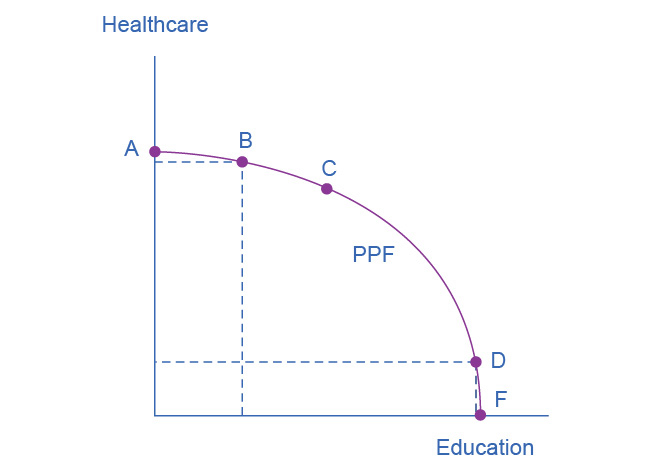
\includegraphics[width=3.25in,height=2.345in]{media/2-2-the-production-possibilities-frontier-and-social-choices_rId23.jpeg}

Figure 2.3 A Healthcare vs.~Education Production Possibilities Frontier
This production possibilities frontier shows a tradeoff between devoting
social resources to healthcare and devoting them to education. At A all
resources go to healthcare and at B, most go to healthcare. At D most
resources go to education, and at F, all go to education.

\protect\hyperlink{CNX_Econ_C02_010}{Figure 2.3} shows healthcare on the
vertical axis and education on the horizontal axis. If the society were
to allocate all of its resources to healthcare, it could produce at
point A. However, it would not have any resources to produce education.
If it were to allocate all of its resources to education, it could
produce at point F. Alternatively, the society could choose to produce
any combination of healthcare and education on the production
possibilities frontier. In effect, the production possibilities frontier
plays the same role for society as the budget constraint plays for
Alphonso. Society can choose any combination of the two goods on or
inside the PPF. However, it does not have enough resources to produce
outside the PPF.

Most importantly, the production possibilities frontier clearly shows
the tradeoff between healthcare and education. Suppose society has
chosen to operate at point B, and it is considering producing more
education. Because the PPF is downward sloping from left to right, the
only way society can obtain more education is by giving up some
healthcare. That is the tradeoff society faces. Suppose it considers
moving from point B to point C. What would the opportunity cost be for
the additional education? The opportunity cost would be the healthcare
society has to forgo. Just as with Alphonso's budget constraint, the
slope of the production possibilities frontier shows the opportunity
cost. By now you might be saying, ``Hey, this PPF is sounding like the
budget constraint.'' If so, read the following Clear It Up feature.

\hypertarget{clear-it-up}{%
\subsection{Clear It Up}\label{clear-it-up}}

\hypertarget{whats-the-difference-between-a-budget-constraint-and-a-ppf}{%
\subsubsection{What's the difference between a budget constraint and a
PPF?}\label{whats-the-difference-between-a-budget-constraint-and-a-ppf}}

There are two major differences between a budget constraint and a
production possibilities frontier. The first is the fact that the budget
constraint is a straight line. This is because its slope is given by the
relative prices of the two goods, which from the point of view of an
individual consumer, are fixed, so the slope doesn\textquotesingle t
change. In contrast, the PPF has a curved shape because of the law of
the diminishing returns. Thus, the slope is different at various points
on the PPF. The second major difference is the absence of specific
numbers on the axes of the PPF. There are no specific numbers because we
do not know the exact amount of resources this imaginary economy has,
nor do we know how many resources it takes to produce healthcare and how
many resources it takes to produce education. If this were a real world
example, that data would be available.

Whether or not we have specific numbers, conceptually we can measure the
opportunity cost of additional education as society moves from point B
to point C on the PPF. We measure the additional education by the
horizontal distance between B and C. The foregone healthcare is given by
the vertical distance between B and C. The slope of the PPF between B
and C is (approximately) the vertical distance (the ``rise'') over the
horizontal distance (the ``run''). This is the opportunity cost of the
additional education.

\hypertarget{the-ppf-and-the-law-of-increasing-opportunity-cost}{%
\subsection{The PPF and the Law of Increasing Opportunity
Cost}\label{the-ppf-and-the-law-of-increasing-opportunity-cost}}

The budget constraints that we presented earlier in this chapter,
showing individual choices about what quantities of goods to consume,
were all straight lines. The reason for these straight lines was that
the relative prices of the two goods in the consumption budget
constraint determined the slope of the budget constraint. However, we
drew the production possibilities frontier for healthcare and education
as a curved line. Why does the PPF have a different shape?

To understand why the PPF is curved, start by considering point A at the
top left-hand side of the PPF. At point A, all available resources are
devoted to healthcare and none are left for education. This situation
would be extreme and even ridiculous. For example, children are seeing a
doctor every day, whether they are sick or not, but not attending
school. People are having cosmetic surgery on every part of their
bodies, but no high school or college education exists. Now imagine that
some of these resources are diverted from healthcare to education, so
that the economy is at point B instead of point A. Diverting some
resources away from A to B causes relatively little reduction in health
because the last few marginal dollars going into healthcare services are
not producing much additional gain in health. However, putting those
marginal dollars into education, which is completely without resources
at point A, can produce relatively large gains. For this reason, the
shape of the PPF from A to B is relatively flat, representing a
relatively small drop-off in health and a relatively large gain in
education.

Now consider the other end, at the lower right, of the production
possibilities frontier. Imagine that society starts at choice D, which
is devoting nearly all resources to education and very few to
healthcare, and moves to point F, which is devoting \emph{all} spending
to education and none to healthcare. For the sake of concreteness, you
can imagine that in the movement from D to F, the last few doctors must
become high school science teachers, the last few nurses must become
school librarians rather than dispensers of vaccinations, and the last
few emergency rooms are turned into kindergartens. The gains to
education from adding these last few resources to education are very
small. However, the opportunity cost lost to health will be fairly
large, and thus the slope of the PPF between D and F is steep, showing a
large drop in health for only a small gain in education.

The lesson is not that society is likely to make an extreme choice like
devoting no resources to education at point A or no resources to health
at point F. Instead, the lesson is that the gains from committing
additional marginal resources to education depend on how much is already
being spent. If on the one hand, very few resources are currently
committed to education, then an increase in resources used for education
can bring relatively large gains. On the other hand, if a large number
of resources are already committed to education, then committing
additional resources will bring relatively smaller gains.

This pattern is common enough that economists have given it a name: the
law of increasing opportunity cost, which holds that as production of a
good or service increases, the marginal opportunity cost of producing it
increases as well. This happens because some resources are better suited
for producing certain goods and services instead of others. When
government spends a certain amount more on reducing crime, for example,
the original increase in opportunity cost of reducing crime could be
relatively small. However, additional increases typically cause
relatively larger increases in the opportunity cost of reducing crime,
and paying for enough police and security to reduce crime to nothing at
all would be a tremendously high opportunity cost.

The curvature of the production possibilities frontier shows that as we
add more resources to education, moving from left to right along the
horizontal axis, the original increase in opportunity cost is fairly
small, but gradually increases. Thus, the slope of the PPF is relatively
flat near the vertical-axis intercept. Conversely, as we add more
resources to healthcare, moving from bottom to top on the vertical axis,
the original declines in opportunity cost are fairly large, but again
gradually diminish. Thus, the slope of the PPF is relatively steep near
the horizontal-axis intercept. In this way, the law of increasing
opportunity cost produces the outward-bending shape of the production
possibilities frontier.

\hypertarget{productive-efficiency-and-allocative-efficiency}{%
\subsection{Productive Efficiency and Allocative
Efficiency}\label{productive-efficiency-and-allocative-efficiency}}

The study of economics does not presume to tell a society what choice it
should make along its production possibilities frontier. In a
market-oriented economy with a democratic government, the choice will
involve a mixture of decisions by individuals, firms, and government.
However, economics can point out that some choices are unambiguously
better than others. This observation is based on the concept of
efficiency. In everyday usage, efficiency refers to lack of waste. An
inefficient machine operates at high cost, while an efficient machine
operates at lower cost, because it is not wasting energy or materials.
An inefficient organization operates with long delays and high costs,
while an efficient organization meets schedules, is focused, and
performs within budget.

The production possibilities frontier can illustrate two kinds of
efficiency: productive efficiency and allocative efficiency.
\protect\hyperlink{CNX_Econ_C02_011}{Figure 2.4} illustrates these ideas
using a production possibilities frontier between healthcare and
education.

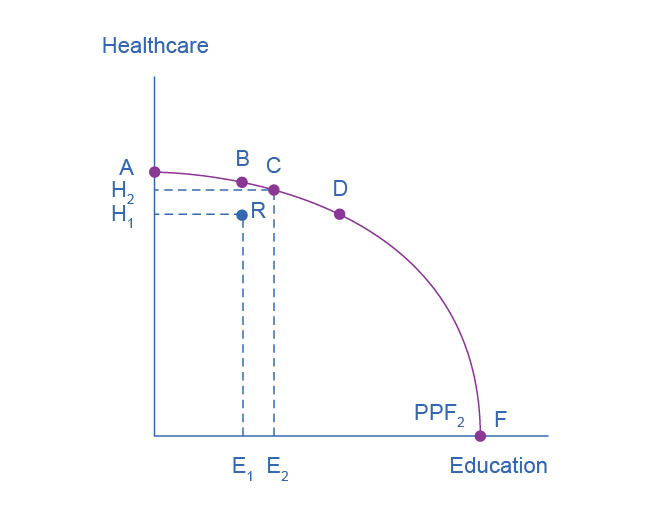
\includegraphics[width=3.25in,height=2.615in]{media/2-2-the-production-possibilities-frontier-and-social-choices_rId33.jpeg}

Figure 2.4 Productive and Allocative Efficiency Productive efficiency
means it is impossible to produce more of one good without decreasing
the quantity that is produced of another good. Thus, all choices along a
given PPF like B, C, and D display productive efficiency, but R does
not. Allocative efficiency means that the particular mix of goods being
produced---that is, the specific choice along the production
possibilities frontier---represents the allocation that society most
desires.

Productive efficiency means that, given the available inputs and
technology, it is impossible to produce more of one good without
decreasing the quantity that is produced of another good. All choices on
the PPF in \protect\hyperlink{CNX_Econ_C02_011}{Figure 2.4}, including
A, B, C, D, and F, display productive efficiency. As a firm moves from
any one of these choices to any other, either healthcare increases and
education decreases or vice versa. However, any choice inside the
production possibilities frontier is productively inefficient and
wasteful because it is possible to produce more of one good, the other
good, or some combination of both goods.

For example, point R is productively inefficient because it is possible
at choice C to have more of both goods: education on the horizontal axis
is higher at point C than point R (E\textsubscript{2} is greater than
E\textsubscript{1}), and healthcare on the vertical axis is also higher
at point C than point R (H\textsubscript{2} is great than
H\textsubscript{1}).

We can show the particular mix of goods and services produced---that is,
the specific combination of selected healthcare and education along the
production possibilities frontier---as a ray (line) from the origin to a
specific point on the PPF. Output mixes that had more healthcare (and
less education) would have a steeper ray, while those with more
education (and less healthcare) would have a flatter ray.

Allocative efficiency means that the particular combination of goods and
services on the production possibility curve that a society produces
represents the combination that society most desires. How to determine
what a society desires can be a controversial question, and is usually a
discussion in political science, sociology, and philosophy classes as
well as in economics. At its most basic, allocative efficiency means
producers supply the quantity of each product that consumers demand.
Only one of the productively efficient choices will be the allocatively
efficient choice for society as a whole.

\hypertarget{why-society-must-choose}{%
\subsection{Why Society Must Choose}\label{why-society-must-choose}}

In
\href{http://openstax.org/books/principles-microeconomics-3e/pages/1-introduction}{Welcome
to Economics!} we learned that every society faces the problem of
scarcity, where limited resources conflict with unlimited needs and
wants. The production possibilities curve illustrates the choices
involved in this dilemma.

Every economy faces two situations in which it may be able to expand
consumption of all goods. In the first case, a society may discover that
it has been using its resources inefficiently, in which case by
improving efficiency and producing on the production possibilities
frontier, it can have more of all goods (or at least more of some and
less of none). In the second case, as resources grow over a period of
years (e.g., more labor and more capital), the economy grows. As it
does, the production possibilities frontier for a society will tend to
shift outward and society will be able to afford more of all goods. In
addition, over time, improvements in technology can increase the level
of production with given resources, and hence push out the PPF.

However, improvements in productive efficiency take time to discover and
implement, and economic growth happens only gradually. Thus, a society
must choose between tradeoffs in the present. For government, this
process often involves trying to identify where additional spending
could do the most good and where reductions in spending would do the
least harm. At the individual and firm level, the market economy
coordinates a process in which firms seek to produce goods and services
in the quantity, quality, and price that people want. However, for both
the government and the market economy in the short term, increases in
production of one good typically mean offsetting decreases somewhere
else in the economy.

\hypertarget{the-ppf-and-comparative-advantage}{%
\subsection{The PPF and Comparative
Advantage}\label{the-ppf-and-comparative-advantage}}

While every society must choose how much of each good or service it
should produce, it does not need to produce every single good it
consumes. Often how much of a good a country decides to produce depends
on how expensive it is to produce it versus buying it from a different
country. As we saw earlier, the curvature of a country's PPF gives us
information about the tradeoff between devoting resources to producing
one good versus another. In particular, its slope gives the opportunity
cost of producing one more unit of the good in the x-axis in terms of
the other good (in the y-axis). Countries tend to have different
opportunity costs of producing a specific good, either because of
different climates, geography, technology, or skills.

Suppose two countries, the US and Brazil, need to decide how much they
will produce of two crops: sugar cane and wheat. Due to its climatic
conditions, Brazil can produce quite a bit of sugar cane per acre but
not much wheat. Conversely, the U.S. can produce large amounts of wheat
per acre, but not much sugar cane. Clearly, Brazil has a lower
opportunity cost of producing sugar cane (in terms of wheat) than the
U.S. The reverse is also true: the U.S. has a lower opportunity cost of
producing wheat than Brazil. We illustrate this by the PPFs of the two
countries in \protect\hyperlink{CNX_Econ_C02_012}{Figure 2.5}.

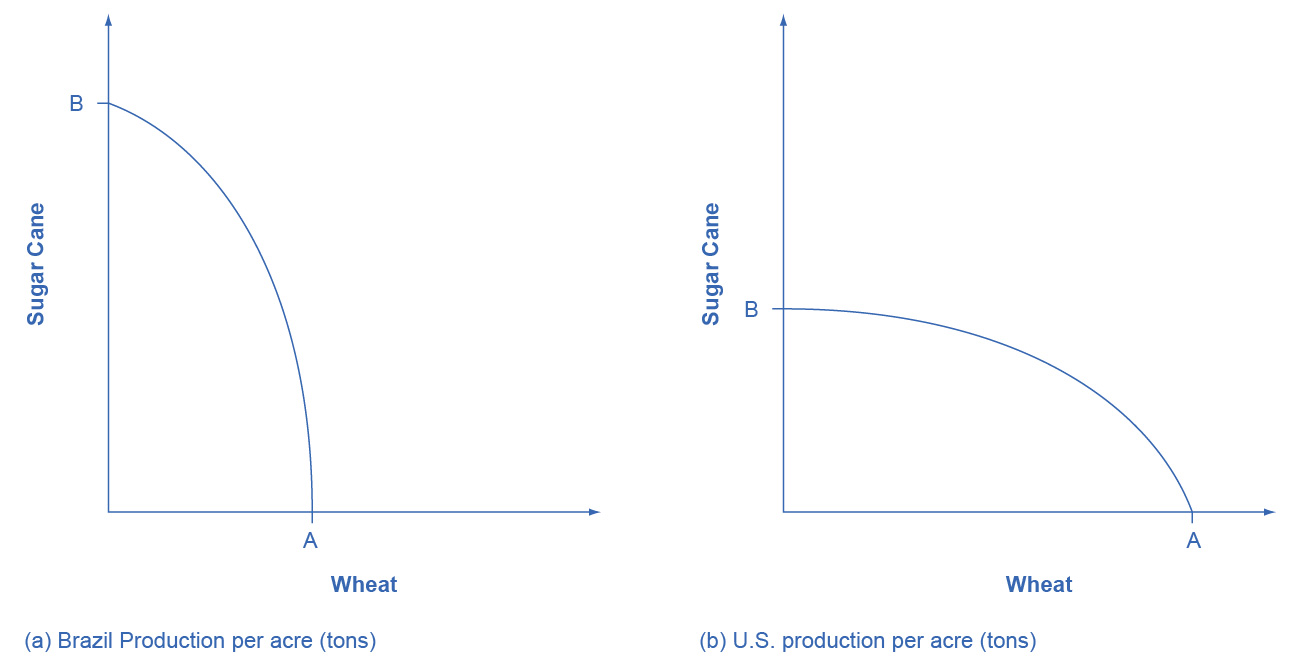
\includegraphics[width=6.5in,height=3.345in]{media/2-2-the-production-possibilities-frontier-and-social-choices_rId45.jpeg}

Figure 2.5 Production Possibility Frontier for the U.S. and Brazil The
U.S. PPF is flatter than the Brazil PPF implying that the opportunity
cost of wheat in terms of sugar cane is lower in the U.S. than in
Brazil. Conversely, the opportunity cost of sugar cane is lower in
Brazil. The U.S. has comparative advantage in wheat and Brazil has
comparative advantage in sugar cane.

When a country can produce a good at a lower opportunity cost than
another country, we say that this country has a comparative advantage in
that good. Comparative advantage is not the same as absolute advantage,
which is when a country can produce more of a good. In our example,
Brazil has an absolute advantage in sugar cane and the U.S. has an
absolute advantage in wheat. One can easily see this with a simple
observation of the extreme production points in the PPFs of the two
countries. If Brazil devoted all of its resources to producing wheat, it
would be producing at point A. If however it had devoted all of its
resources to producing sugar cane instead, it would be producing a much
larger amount than the U.S., at point B.

The slope of the PPF gives the opportunity cost of producing an
additional unit of wheat. While the slope is not constant throughout the
PPFs, it is quite apparent that the PPF in Brazil is much steeper than
in the U.S., and therefore the opportunity cost of wheat is generally
higher in Brazil. In the chapter on
\href{http://openstax.org/books/principles-microeconomics-3e/pages/19-introduction-to-international-trade}{International
Trade} you will learn that countries' differences in comparative
advantage determine which goods they will choose to produce and trade.
When countries engage in trade, they specialize in the production of the
goods in which they have comparative advantage, and trade part of that
production for goods in which they do not have comparative advantage.
With trade, manufacturers produce goods where the opportunity cost is
lowest, so total production increases, benefiting both trading parties.

\hypertarget{confronting-objections-to-the-economic-approach}{%
\chapter{2.3 Confronting Objections to the Economic
Approach}\label{confronting-objections-to-the-economic-approach}}

\hypertarget{learning-objectives-6}{%
\subsection{Learning Objectives}\label{learning-objectives-6}}

By the end of this section, you will be able to:

\begin{itemize}
\tightlist
\item
  Analyze arguments against economic approaches to decision-making
\item
  Interpret a tradeoff diagram
\item
  Contrast normative statements and positive statements
\end{itemize}

It is one thing to understand the economic approach to decision-making
and another thing to feel comfortable applying it. The sources of
discomfort typically fall into two categories: that people do not act in
the way that fits the economic way of thinking, and that even if people
did act that way, they should try not to. Let's consider these arguments
in turn.

\hypertarget{first-objection-people-firms-and-society-do-not-act-like-this}{%
\subsection{First Objection: People, Firms, and Society Do Not Act Like
This}\label{first-objection-people-firms-and-society-do-not-act-like-this}}

The economic approach to decision-making seems to require more
information than most individuals possess and more careful
decision-making than most individuals actually display. After all, do
you or any of your friends draw a budget constraint and mutter to
yourself about maximizing utility before you head to the shopping mall?
Do members of the U.S. Congress contemplate production possibilities
frontiers before they vote on the annual budget? The messy ways in which
people and societies operate somehow doesn't look much like neat budget
constraints or smoothly curving production possibilities frontiers.

However, the economics approach can be a useful way to analyze and
understand the tradeoffs of economic decisions. To appreciate this
point, imagine for a moment that you are playing basketball, dribbling
to the right, and throwing a bounce-pass to the left to a teammate who
is running toward the basket. A physicist or engineer could work out the
correct speed and trajectory for the pass, given the different movements
involved and the weight and bounciness of the ball. However, when you
are playing basketball, you do not perform any of these calculations.
You just pass the ball, and if you are a good player, you will do so
with high accuracy.

Someone might argue: ``The scientist's formula of the bounce-pass
requires a far greater knowledge of physics and far more specific
information about speeds of movement and weights than the basketball
player actually has, so it must be an unrealistic description of how
basketball passes actually occur.'' This reaction would be wrongheaded.
The fact that a good player can throw the ball accurately because of
practice and skill, without making a physics calculation, does not mean
that the physics calculation is wrong.

Similarly, from an economic point of view, someone who shops for
groceries every week has a great deal of practice with how to purchase
the combination of goods that will provide that person with utility,
even if the shopper does not phrase decisions in terms of a budget
constraint. Government institutions may work imperfectly and slowly, but
in general, a democratic form of government feels pressure from voters
and social institutions to make the choices that are most widely
preferred by people in that society. Thus, when thinking about the
economic actions of groups of people, firms, and society, it is
reasonable, as a first approximation, to analyze them with the tools of
economic analysis. For more on this, read about behavioral economics in
the chapter on
\href{http://openstax.org/books/principles-microeconomics-3e/pages/6-introduction-to-consumer-choices}{Consumer
Choices}.

\hypertarget{second-objection-people-firms-and-society-should-not-act-this-way}{%
\subsection{Second Objection: People, Firms, and Society Should Not Act
This
Way}\label{second-objection-people-firms-and-society-should-not-act-this-way}}

The economics approach portrays people as self-interested. For some
critics of this approach, even if self-interest is an accurate
description of how people behave, these behaviors are not moral.
Instead, the critics argue that people should be taught to care more
deeply about others. Economists offer several answers to these concerns.

First, economics is not a form of moral instruction. Rather, it seeks to
describe economic behavior as it actually exists. Philosophers draw a
distinction between positive statements, which describe the world as it
is, and normative statements, which describe how the world should be.
Positive statements are factual. They may be true or false, but we can
test them, at least in principle. Normative statements are subjective
questions of opinion. We cannot test them since we cannot prove opinions
to be true or false. They just are opinions based on
one\textquotesingle s values. For example, an economist could analyze a
proposed subway system in a certain city. If the expected benefits
exceed the costs, he concludes that the project is worthy---an example
of positive analysis. Another economist argues for extended unemployment
compensation during the COVID-19 pandemic because a rich country like
the United States should take care of its less fortunate citizens---an
example of normative analysis.

Even if the line between positive and normative statements is not always
crystal clear, economic analysis does try to remain rooted in the study
of the actual people who inhabit the actual economy. Fortunately
however, the assumption that individuals are purely self-interested is a
simplification about human nature. In fact, we need to look no further
than to Adam Smith, the very father of modern economics to find evidence
of this. The opening sentence of his book, \emph{The Theory of Moral
Sentiments}, puts it very clearly: ``How selfish soever man may be
supposed, there are evidently some principles in his nature, which
interest him in the fortune of others, and render their happiness
necessary to him, though he derives nothing from it except the pleasure
of seeing it.'' Clearly, individuals are both self-interested and
altruistic.

Second, we can label self-interested behavior and profit-seeking with
other names, such as personal choice and freedom. The ability to make
personal choices about buying, working, and saving is an important
personal freedom. Some people may choose high-pressure, high-paying jobs
so that they can earn and spend considerable amounts of money on
themselves. Others may allocate large portions of their earnings to
charity or spend it on their friends and family. Others may devote
themselves to a career that can require much time, energy, and expertise
but does not offer high financial rewards, like being an elementary
school teacher or a social worker. Still others may choose a job that
does consume much of their time or provide a high level of income, but
still leaves time for family, friends, and contemplation. Some people
may prefer to work for a large company; others might want to start their
own business. People's freedom to make their own economic choices has a
moral value worth respecting.

\hypertarget{clear-it-up}{%
\subsection{Clear It Up}\label{clear-it-up}}

\hypertarget{is-a-diagram-by-any-other-name-the-same}{%
\subsubsection{Is a diagram by any other name the
same?}\label{is-a-diagram-by-any-other-name-the-same}}

When you study economics, you may feel buried under an avalanche of
diagrams. Your goal should be to recognize the common underlying logic
and pattern of the diagrams, not to memorize each one.

This chapter uses only one basic diagram, although we present it with
different sets of labels. The consumption budget constraint and the
production possibilities frontier for society, as a whole, are the same
basic diagram. \protect\hyperlink{CNX_Econ_C02_014}{Figure 2.6} shows an
individual budget constraint and a production possibilities frontier for
two goods, Good 1 and Good 2. The tradeoff diagram always illustrates
three basic themes: scarcity, tradeoffs, and economic efficiency.

The first theme is scarcity. It is not feasible to have unlimited
amounts of both goods. Even if the budget constraint or a PPF shifts,
scarcity remains---just at a different level. The second theme is
tradeoffs. As depicted in the budget constraint or the production
possibilities frontier, it is necessary to forgo some of one good to
gain more of the other good. The details of this tradeoff vary. In a
budget constraint we determine, the tradeoff is determined by the
relative prices of the goods: that is, the relative price of two goods
in the consumption choice budget constraint. These tradeoffs appear as a
straight line. However, a curved line represents the tradeoffs in many
production possibilities frontiers because the law of diminishing
returns holds that as we add resources to an area, the marginal gains
tend to diminish. Regardless of the specific shape, tradeoffs remain.

The third theme is economic efficiency, or getting the most benefit from
scarce resources. All choices on the production possibilities frontier
show productive efficiency because in such cases, there is no way to
increase the quantity of one good without decreasing the quantity of the
other. Similarly, when an individual makes a choice along a budget
constraint, there is no way to increase the quantity of one good without
decreasing the quantity of the other. The choice on a production
possibilities set that is socially preferred, or the choice on an
individual's budget constraint that is personally preferred, will
display allocative efficiency.

The basic budget constraint/production possibilities frontier diagram
will recur throughout this book. Some examples include using these
tradeoff diagrams to analyze trade, environmental protection and
economic output, equality of incomes and economic output, and the
macroeconomic tradeoff between consumption and investment. Do not allow
the different labels to confuse you. The budget constraint/production
possibilities frontier diagram is always just a tool for thinking
carefully about scarcity, tradeoffs, and efficiency in a particular
situation.

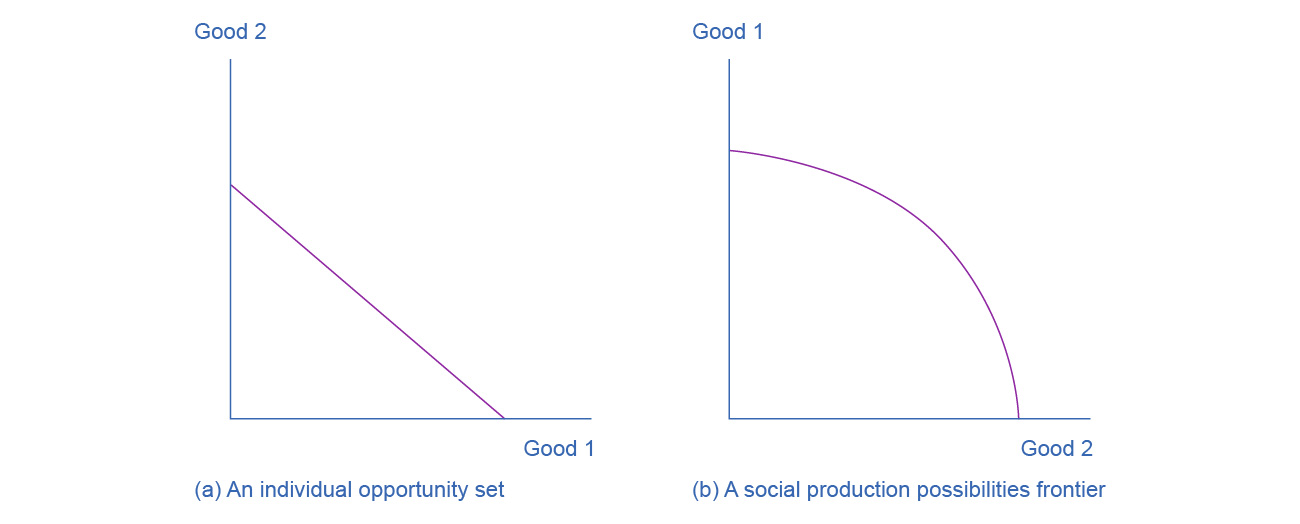
\includegraphics[width=6.5in,height=2.62in]{media/2-3-confronting-objections-to-the-economic-approach_rId31.jpeg}

Figure 2.6 The Tradeoff Diagram Both the individual opportunity set (or
budget constraint) and the social production possibilities frontier show
the constraints under which individual consumers and society as a whole
operate. Both diagrams show the tradeoff in choosing more of one good at
the cost of less of the other.

Third, self-interested behavior can lead to positive social results. For
example, when people work hard to make a living, they create economic
output. Consumers who are looking for the best deals will encourage
businesses to offer goods and services that meet their needs. Adam
Smith, writing in \emph{The Wealth of Nations}, named this property the
invisible hand. In describing how consumers and producers interact in a
market economy, Smith wrote:

\begin{quote}
Every individual\ldots generally, indeed, neither intends to promote the
public interest, nor knows how much he is promoting it. By preferring
the support of domestic to that of foreign industry, he intends only his
own security; and by directing that industry in such a manner as its
produce may be of the greatest value, he intends only his own gain. And
he is in this, as in many other cases, led by an invisible hand to
promote an end which was no part of his intention\ldots By pursuing his
own interest he frequently promotes that of the society more effectually
than when he really intends to promote it.
\end{quote}

The metaphor of the invisible hand suggests the remarkable possibility
that broader social good can emerge from selfish individual actions.

Fourth, even people who focus on their own self-interest in the economic
part of their life often set aside their own narrow self-interest in
other parts of life. For example, you might focus on your own
self-interest when asking your employer for a raise or negotiating to
buy a car. Then you might turn around and focus on other people when you
volunteer to read stories at the local library, help a friend move to a
new apartment, or donate money to a charity. Self-interest is a
reasonable starting point for analyzing many economic decisions, without
needing to imply that people never do anything that is not in their own
immediate self-interest.

\hypertarget{bring-it-home}{%
\subsection{Bring It Home}\label{bring-it-home}}

\hypertarget{choices-...-to-what-degree}{%
\subsubsection{Choices ... to What
Degree?}\label{choices-...-to-what-degree}}

What have we learned? We know that scarcity impacts all the choices we
make. An economist might argue that people do not obtain a bachelor's or
master's degree because they do not have the resources to make those
choices or because their incomes are too low and/or the price of these
degrees is too high. A bachelor's or a master's degree may not be
available in their opportunity set.

The price of these degrees may be too high not only because the actual
price, college tuition (and perhaps room and board), is too high. An
economist might also say that for many people, the full opportunity cost
of a bachelor's or a master's degree is too high. For these people, they
are unwilling or unable to make the tradeoff of forfeiting years of
working, and earning an income, to earn a degree.

Finally, the statistics we introduced at the start of the chapter reveal
information about intertemporal choices. An economist might say that
people choose not to obtain a college degree because they may have to
borrow money to attend college, and the interest they have to pay on
that loan in the future will affect their decisions today. Also, it
could be that some people have a preference for current consumption over
future consumption, so they choose to work now at a lower salary and
consume now, rather than postponing that consumption until after they
graduate college.

\part{3-Demand and Supply}

\hypertarget{chapter-objectives}{%
\chapter{Chapter Objectives}\label{chapter-objectives}}

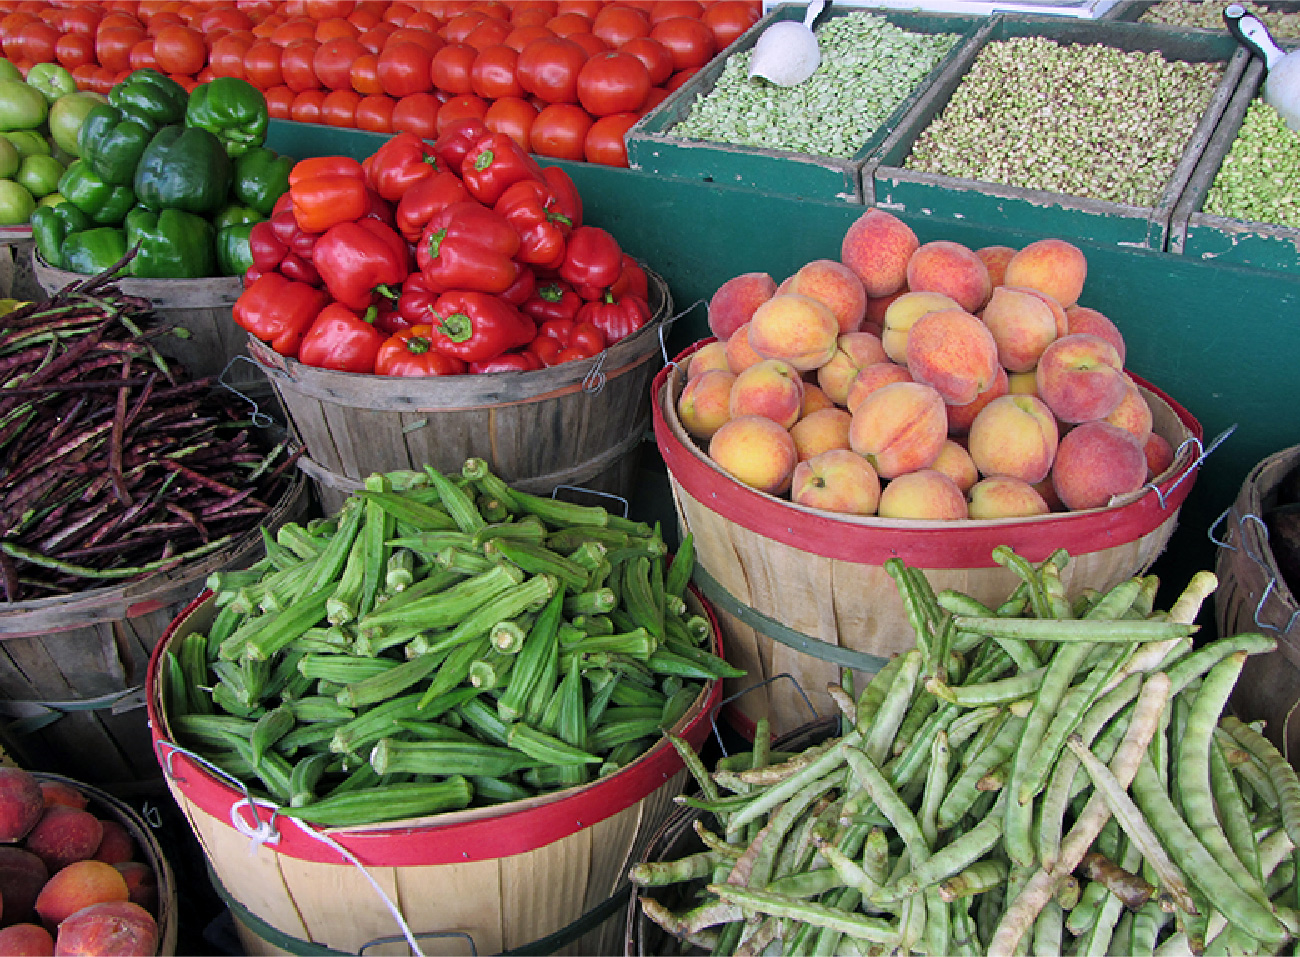
\includegraphics[width=6.5in,height=4.785in]{media/3-introduction-to-demand-and-supply_rId20.jpeg}

Figure 3.1 Farmer's Market Organic vegetables and fruits that are grown
and sold within a specific geographical region should, in theory, cost
less than conventional produce because the transportation costs are
less. That is not, however, usually the case. (Credit: modification of
"Old Farmers\textquotesingle{} Market" by NatalieMaynor/Flickr, CC BY
2.0)

In this chapter, you will learn about:

\begin{itemize}
\tightlist
\item
  Demand, Supply, and Equilibrium in Markets for Goods and Services
\item
  Shifts in Demand and Supply for Goods and Services
\item
  Changes in Equilibrium Price and Quantity: The Four-Step Process
\item
  Price Ceilings and Price Floors
\end{itemize}

\hypertarget{introduction-to-demand-and-supply}{%
\section{Introduction to Demand and
Supply}\label{introduction-to-demand-and-supply}}

\hypertarget{bring-it-home}{%
\subsection{Bring It Home}\label{bring-it-home}}

\hypertarget{why-can-we-not-get-enough-of-organic-foods}{%
\subsubsection{Why Can We Not Get Enough of Organic
Foods?}\label{why-can-we-not-get-enough-of-organic-foods}}

Organic food is increasingly popular, not just in the United States, but
worldwide. At one time, consumers had to go to specialty stores or
farmers\textquotesingle{} markets to find organic produce. Now it is
available in most grocery stores. In short, organic has become part of
the mainstream.

Ever wonder why organic food costs more than conventional food? Why,
say, does an organic Fuji apple cost \$2.75 a pound, while its
conventional counterpart costs \$1.72 a pound? The same price
relationship is true for just about every organic product on the market.
If many organic foods are locally grown, would they not take less time
to get to market and therefore be cheaper? What are the forces that keep
those prices from coming down? Turns out those forces have quite a bit
to do with this chapter's topic: demand and supply.

An auction bidder pays thousands of dollars for a dress Whitney Houston
wore. A collector spends a small fortune for a few drawings by John
Lennon. People usually react to purchases like these in two ways: their
jaw drops because they think these are high prices to pay for such goods
or they think these are rare, desirable items and the amount paid seems
right.

\hypertarget{link-it-up}{%
\subsection{Link It Up}\label{link-it-up}}

Visit this \href{http://openstax.org/l/celebauction}{website} to read a
list of bizarre items that have been purchased for their ties to
celebrities. These examples represent an interesting facet of demand and
supply.

When economists talk about prices, they are less interested in making
judgments than in gaining a practical understanding of what determines
prices and why prices change. Consider a price most of us contend with
weekly: that of a gallon of gas. Why was the average price of gasoline
in the United States \$3.16 per gallon in June of 2020? Why did the
price for gasoline fall sharply to \$2.42 per gallon by January of 2021?
To explain these price movements, economists focus on the determinants
of what gasoline buyers are willing to pay and what gasoline sellers are
willing to accept.

As it turns out, the price of gasoline in June of any given year is
nearly always higher than the price in January of that same year. Over
recent decades, gasoline prices in midsummer have averaged about 10
cents per gallon more than their midwinter low. The likely reason is
that people drive more in the summer, and are also willing to pay more
for gas, but that does not explain how steeply gas prices fell. Other
factors were at work during those 18 months, such as increases in supply
and decreases in the demand for crude oil.

This chapter introduces the economic model of demand and supply---one of
the most powerful models in all of economics. The discussion here begins
by examining how demand and supply determine the price and the quantity
sold in markets for goods and services, and how changes in demand and
supply lead to changes in prices and quantities.

\hypertarget{demand-supply-and-equilibrium-in-markets-for-goods-and-services}{%
\chapter{3.1 Demand, Supply, and Equilibrium in Markets for Goods and
Services}\label{demand-supply-and-equilibrium-in-markets-for-goods-and-services}}

\hypertarget{learning-objectives-7}{%
\subsection{Learning Objectives}\label{learning-objectives-7}}

By the end of this section, you will be able to:

\begin{itemize}
\tightlist
\item
  Explain demand, quantity demanded, and the law of demand
\item
  Explain supply, quantity supplied, and the law of supply
\item
  Identify a demand curve and a supply curve
\item
  Explain equilibrium, equilibrium price, and equilibrium quantity
\end{itemize}

First let's first focus on what economists mean by demand, what they
mean by supply, and then how demand and supply interact in a market.

\hypertarget{demand-for-goods-and-services}{%
\subsection{Demand for Goods and
Services}\label{demand-for-goods-and-services}}

Economists use the term demand to refer to the amount of some good or
service consumers are willing and able to purchase at each price. Demand
is fundamentally based on needs and wants---if you have no need or want
for something, you won't buy it. While a consumer may be able to
differentiate between a need and a want, from an economist's perspective
they are the same thing. Demand is also based on ability to pay. If you
cannot pay for it, you have no effective demand. By this definition, a
person who does not have a drivers license has no effective demand for a
car.

What a buyer pays for a unit of the specific good or service is called
price. The total number of units that consumers would purchase at that
price is called the quantity demanded. A rise in price of a good or
service almost always decreases the quantity demanded of that good or
service. Conversely, a fall in price will increase the quantity
demanded. When the price of a gallon of gasoline increases, for example,
people look for ways to reduce their consumption by combining several
errands, commuting by carpool or mass transit, or taking weekend or
vacation trips closer to home. Economists call this inverse relationship
between price and quantity demanded the law of demand. The law of demand
assumes that all other variables that affect demand (which we explain in
the next module) are held constant.

We can show an example from the market for gasoline in a table or a
graph. Economist call a table that shows the quantity demanded at each
price, such as \protect\hyperlink{Table_03_01}{Table 3.1}, a demand
schedule. In this case we measure price in dollars per gallon of
gasoline. We measure the quantity demanded in millions of gallons over
some time period (for example, per day or per year) and over some
geographic area (like a state or a country). A demand curve shows the
relationship between price and quantity demanded on a graph like
\protect\hyperlink{CNX_Econ_C03_001}{Figure 3.2}, with quantity on the
horizontal axis and the price per gallon on the vertical axis. (Note
that this is an exception to the normal rule in mathematics that the
independent variable (x) goes on the horizontal axis and the dependent
variable (y) goes on the vertical axis. Economics is not math.)

\protect\hyperlink{Table_03_01}{Table 3.1} shows the demand schedule and
the graph in \protect\hyperlink{CNX_Econ_C03_001}{Figure 3.2} shows the
demand curve. These are two ways to describe the same relationship
between price and quantity demanded.

Table 3.1 Price and Quantity Demanded of Gasoline

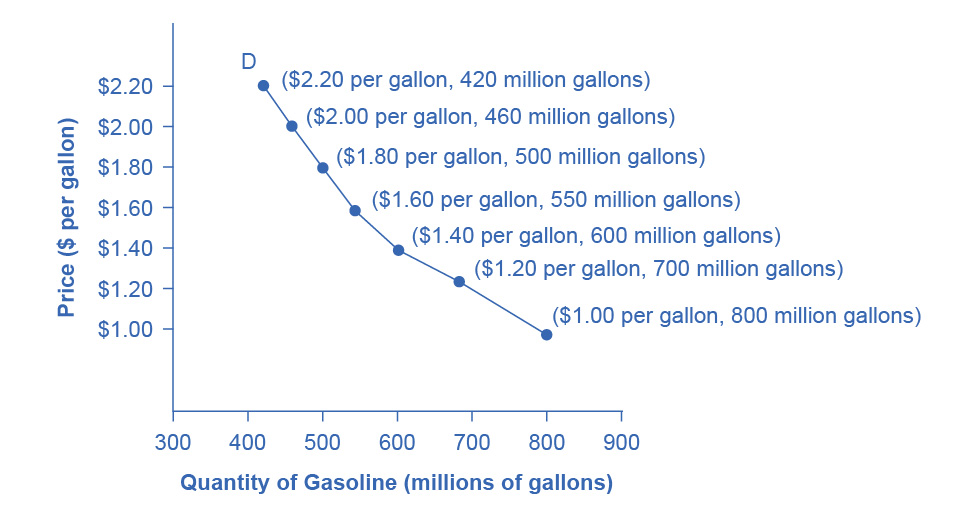
\includegraphics[width=4.88in,height=2.61in]{media/3-1-demand-supply-and-equilibrium-in-markets-for-goods-and-services_rId28.jpeg}

Figure 3.2 A Demand Curve for Gasoline The demand schedule shows that as
price rises, quantity demanded decreases, and vice versa. We graph these
points, and the line connecting them is the demand curve (D). The
downward slope of the demand curve again illustrates the law of
demand---the inverse relationship between prices and quantity demanded.

Demand curves will appear somewhat different for each product. They may
appear relatively steep or flat, or they may be straight or curved.
Nearly all demand curves share the fundamental similarity that they
slope down from left to right. Demand curves embody the law of demand:
As the price increases, the quantity demanded decreases, and conversely,
as the price decreases, the quantity demanded increases.

Confused about these different types of demand? Read the next Clear It
Up feature.

\hypertarget{clear-it-up}{%
\subsection{Clear It Up}\label{clear-it-up}}

\hypertarget{is-demand-the-same-as-quantity-demanded}{%
\subsubsection{Is demand the same as quantity
demanded?}\label{is-demand-the-same-as-quantity-demanded}}

In economic terminology, demand is not the same as quantity demanded.
When economists talk about demand, they mean the relationship between a
range of prices and the quantities demanded at those prices, as
illustrated by a demand curve or a demand schedule. When economists talk
about quantity demanded, they mean only a certain point on the demand
curve, or one quantity on the demand schedule. In short, demand refers
to the curve and quantity demanded refers to a (specific) point on the
curve.

\hypertarget{supply-of-goods-and-services}{%
\subsection{Supply of Goods and
Services}\label{supply-of-goods-and-services}}

When economists talk about supply, they mean the amount of some good or
service a producer is willing to supply at each price. Price is what the
producer receives for selling one unit of a good or service. A rise in
price almost always leads to an increase in the quantity supplied of
that good or service, while a fall in price will decrease the quantity
supplied. When the price of gasoline rises, for example, it encourages
profit-seeking firms to take several actions: expand exploration for oil
reserves; drill for more oil; invest in more pipelines and oil tankers
to bring the oil to plants for refining into gasoline; build new oil
refineries; purchase additional pipelines and trucks to ship the
gasoline to gas stations; and open more gas stations or keep existing
gas stations open longer hours. Economists call this positive
relationship between price and quantity supplied---that a higher price
leads to a higher quantity supplied and a lower price leads to a lower
quantity supplied---the law of supply. The law of supply assumes that
all other variables that affect supply (to be explained in the next
module) are held constant.

Still unsure about the different types of supply? See the following
Clear It Up feature.

\hypertarget{clear-it-up-1}{%
\subsection{Clear It Up}\label{clear-it-up-1}}

\hypertarget{is-supply-the-same-as-quantity-supplied}{%
\subsubsection{Is supply the same as quantity
supplied?}\label{is-supply-the-same-as-quantity-supplied}}

In economic terminology, supply is not the same as quantity supplied.
When economists refer to supply, they mean the relationship between a
range of prices and the quantities supplied at those prices, a
relationship that we can illustrate with a supply curve or a supply
schedule. When economists refer to quantity supplied, they mean only a
certain point on the supply curve, or one quantity on the supply
schedule. In short, supply refers to the curve and quantity supplied
refers to a (specific) point on the curve.

\protect\hyperlink{CNX_Econ_C03_002}{Figure 3.3} illustrates the law of
supply, again using the market for gasoline as an example. Like demand,
we can illustrate supply using a table or a graph. A supply schedule is
a table, like \protect\hyperlink{Table_03_02}{Table 3.2}, that shows the
quantity supplied at a range of different prices. Again, we measure
price in dollars per gallon of gasoline and we measure quantity supplied
in millions of gallons. A supply curve is a graphic illustration of the
relationship between price, shown on the vertical axis, and quantity,
shown on the horizontal axis. The supply schedule and the supply curve
are just two different ways of showing the same information. Notice that
the horizontal and vertical axes on the graph for the supply curve are
the same as for the demand curve.

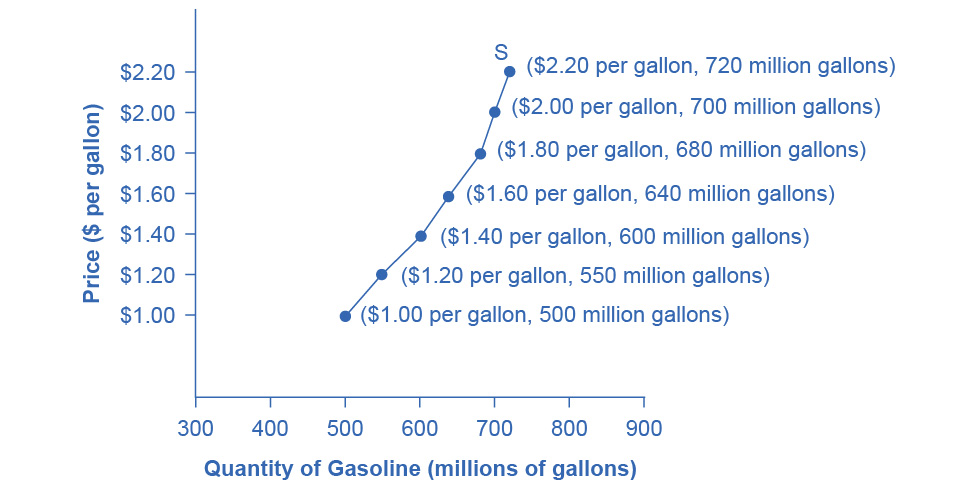
\includegraphics[width=4.88in,height=2.47in]{media/3-1-demand-supply-and-equilibrium-in-markets-for-goods-and-services_rId42.jpeg}

Figure 3.3 A Supply Curve for Gasoline The supply schedule is the table
that shows quantity supplied of gasoline at each price. As price rises,
quantity supplied also increases, and vice versa. The supply curve (S)
is created by graphing the points from the supply schedule and then
connecting them. The upward slope of the supply curve illustrates the
law of supply---that a higher price leads to a higher quantity supplied,
and vice versa.

Table 3.2 Price and Supply of Gasoline

The shape of supply curves will vary somewhat according to the product:
steeper, flatter, straighter, or curved. Nearly all supply curves,
however, share a basic similarity: they slope up from left to right and
illustrate the law of supply: as the price rises, say, from \$1.00 per
gallon to \$2.20 per gallon, the quantity supplied increases from 500
gallons to 720 gallons. Conversely, as the price falls, the quantity
supplied decreases.

\hypertarget{equilibriumwhere-demand-and-supply-intersect}{%
\subsection{Equilibrium---Where Demand and Supply
Intersect}\label{equilibriumwhere-demand-and-supply-intersect}}

Because the graphs for demand and supply curves both have price on the
vertical axis and quantity on the horizontal axis, the demand curve and
supply curve for a particular good or service can appear on the same
graph. Together, demand and supply determine the price and the quantity
that will be bought and sold in a market.

\protect\hyperlink{CNX_Econ_C03_003}{Figure 3.4} illustrates the
interaction of demand and supply in the market for gasoline. The demand
curve (D) is identical to \protect\hyperlink{CNX_Econ_C03_001}{Figure
3.2}. The supply curve (S) is identical to
\protect\hyperlink{CNX_Econ_C03_002}{Figure 3.3}.
\protect\hyperlink{Table_03_03}{Table 3.3} contains the same information
in tabular form.

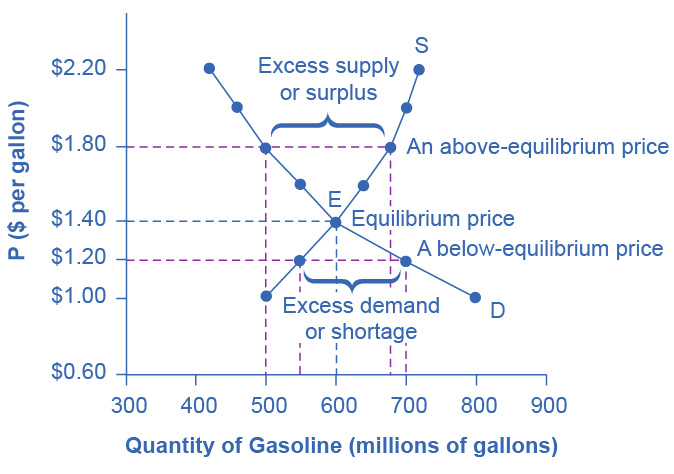
\includegraphics[width=3.37in,height=2.37in]{media/3-1-demand-supply-and-equilibrium-in-markets-for-goods-and-services_rId47.jpeg}

Figure 3.4 Demand and Supply for Gasoline The demand curve (D) and the
supply curve (S) intersect at the equilibrium point E, with a price of
\$1.40 and a quantity of 600. The equilibrium price is the only price
where quantity demanded is equal to quantity supplied. At a price above
equilibrium like \$1.80, quantity supplied exceeds the quantity
demanded, so there is excess supply. At a price below equilibrium such
as \$1.20, quantity demanded exceeds quantity supplied, so there is
excess demand.

Table 3.3 Price, Quantity Demanded, and Quantity Supplied

Remember this: When two lines on a diagram cross, this intersection
usually means something. The point where the supply curve (S) and the
demand curve (D) cross, designated by point E in
\protect\hyperlink{CNX_Econ_C03_003}{Figure 3.4}, is called the
equilibrium. The equilibrium price is the only price where the plans of
consumers and the plans of producers agree---that is, where the amount
of the product consumers want to buy (quantity demanded) is equal to the
amount producers want to sell (quantity supplied). Economists call this
common quantity the equilibrium quantity. At any other price, the
quantity demanded does not equal the quantity supplied, so the market is
not in equilibrium at that price.

In \protect\hyperlink{CNX_Econ_C03_003}{Figure 3.4}, the equilibrium
price is \$1.40 per gallon of gasoline and the equilibrium quantity is
600 million gallons. If you had only the demand and supply schedules,
and not the graph, you could find the equilibrium by looking for the
price level on the tables where the quantity demanded and the quantity
supplied are equal.

The word ``equilibrium'' means ``balance.'' If a market is at its
equilibrium price and quantity, then it has no reason to move away from
that point. However, if a market is not at equilibrium, then economic
pressures arise to move the market toward the equilibrium price and the
equilibrium quantity.

Imagine, for example, that the price of a gallon of gasoline was above
the equilibrium price---that is, instead of \$1.40 per gallon, the price
is \$1.80 per gallon. The dashed horizontal line at the price of \$1.80
in \protect\hyperlink{CNX_Econ_C03_003}{Figure 3.4} illustrates this
above-equilibrium price. At this higher price, the quantity demanded
drops from 600 to 500. This decline in quantity reflects how consumers
react to the higher price by finding ways to use less gasoline.

Moreover, at this higher price of \$1.80, the quantity of gasoline
supplied rises from 600 to 680, as the higher price makes it more
profitable for gasoline producers to expand their output. Now, consider
how quantity demanded and quantity supplied are related at this
above-equilibrium price. Quantity demanded has fallen to 500 gallons,
while quantity supplied has risen to 680 gallons. In fact, at any
above-equilibrium price, the quantity supplied exceeds the quantity
demanded. We call this an excess supply or a surplus.

With a surplus, gasoline accumulates at gas stations, in tanker trucks,
in pipelines, and at oil refineries. This accumulation puts pressure on
gasoline sellers. If a surplus remains unsold, those firms involved in
making and selling gasoline are not receiving enough cash to pay their
workers and to cover their expenses. In this situation, some producers
and sellers will want to cut prices, because it is better to sell at a
lower price than not to sell at all. Once some sellers start cutting
prices, others will follow to avoid losing sales. These price reductions
in turn will stimulate a higher quantity demanded. Therefore, if the
price is above the equilibrium level, incentives built into the
structure of demand and supply will create pressures for the price to
fall toward the equilibrium.

Now suppose that the price is below its equilibrium level at \$1.20 per
gallon, as the dashed horizontal line at this price in
\protect\hyperlink{CNX_Econ_C03_003}{Figure 3.4} shows. At this lower
price, the quantity demanded increases from 600 to 700 as drivers take
longer trips, spend more minutes warming up the car in the driveway in
wintertime, stop sharing rides to work, and buy larger cars that get
fewer miles to the gallon. However, the below-equilibrium price reduces
gasoline producers' incentives to produce and sell gasoline, and the
quantity supplied falls from 600 to 550.

When the price is below equilibrium, there is excess demand, or a
shortage---that is, at the given price the quantity demanded, which has
been stimulated by the lower price, now exceeds the quantity supplied,
which has been depressed by the lower price. In this situation, eager
gasoline buyers mob the gas stations, only to find many stations running
short of fuel. Oil companies and gas stations recognize that they have
an opportunity to make higher profits by selling what gasoline they have
at a higher price. As a result, the price rises toward the equilibrium
level. Read
\href{http://openstax.org/books/principles-microeconomics-3e/pages/3-5-demand-supply-and-efficiency}{Demand,
Supply, and Efficiency} for more discussion on the importance of the
demand and supply model.

\hypertarget{shifts-in-demand-and-supply-for-goods-and-services}{%
\chapter{3.2 Shifts in Demand and Supply for Goods and
Services}\label{shifts-in-demand-and-supply-for-goods-and-services}}

\hypertarget{learning-objectives-8}{%
\subsection{Learning Objectives}\label{learning-objectives-8}}

By the end of this section, you will be able to:

\begin{itemize}
\tightlist
\item
  Identify factors that affect demand
\item
  Graph demand curves and demand shifts
\item
  Identify factors that affect supply
\item
  Graph supply curves and supply shifts
\end{itemize}

The previous module explored how price affects the quantity demanded and
the quantity supplied. The result was the demand curve and the supply
curve. Price, however, is not the only factor that influences buyers'
and sellers' decisions. For example, how is demand for vegetarian food
affected if, say, health concerns cause more consumers to avoid eating
meat? How is the supply of diamonds affected if diamond producers
discover several new diamond mines? What are the major factors, in
addition to the price, that influence demand or supply?

\hypertarget{link-it-up}{%
\subsection{Link It Up}\label{link-it-up}}

Visit this \href{https://openstax.org/l/toothfish}{website} to read a
brief note on how marketing strategies can influence supply and demand
of products.

\hypertarget{what-factors-affect-demand}{%
\subsection{What Factors Affect
Demand?}\label{what-factors-affect-demand}}

We defined demand as the amount of some product a consumer is willing
and able to purchase at each price. That suggests at least two factors
that affect demand. Willingness to purchase suggests a desire, based on
what economists call tastes and preferences. If you neither need nor
want something, you will not buy it, and if you really like something,
you will buy more of it than someone who does not share your strong
preference for it. Ability to purchase suggests that income is
important. Professors are usually able to afford better housing and
transportation than students, because they have more income. Prices of
related goods can affect demand also. If you need a new car, the price
of a Honda may affect your demand for a Ford. Finally, the size or
composition of the population can affect demand. The more children a
family has, the greater their demand for clothing. The more driving-age
children a family has, the greater their demand for car insurance, and
the less for diapers and baby formula.

These factors matter for both individual and market demand as a whole.
Exactly how do these various factors affect demand, and how do we show
the effects graphically? To answer those questions, we need the
\emph{ceteris paribus} assumption.

\hypertarget{the-ceteris-paribus-assumption}{%
\subsection{\texorpdfstring{The \emph{Ceteris Paribus}
Assumption}{The Ceteris Paribus Assumption}}\label{the-ceteris-paribus-assumption}}

A demand curve or a supply curve is a relationship between two, and only
two, variables: quantity on the horizontal axis and price on the
vertical axis. The assumption behind a demand curve or a supply curve is
that no relevant economic factors, other than the product's price, are
changing. Economists call this assumption ceteris paribus, a Latin
phrase meaning ``other things being equal.'' Any given demand or supply
curve is based on the \emph{ceteris paribus} assumption that all else is
held equal. A demand curve or a supply curve is a relationship between
two, and only two, variables when all other variables are kept constant.
If all else is not held equal, then the laws of supply and demand will
not necessarily hold, as the following Clear It Up feature shows.

\hypertarget{clear-it-up}{%
\subsection{Clear It Up}\label{clear-it-up}}

\hypertarget{when-does-ceteris-paribus-apply}{%
\subsubsection{\texorpdfstring{When does \emph{ceteris paribus}
apply?}{When does ceteris paribus apply?}}\label{when-does-ceteris-paribus-apply}}

We typically apply \emph{ceteris paribus} when we observe how changes in
price affect demand or supply, but we can apply \emph{ceteris paribus}
more generally. In the real world, demand and supply depend on more
factors than just price. For example, a consumer's demand depends on
income and a producer's supply depends on the cost of producing the
product. How can we analyze the effect on demand or supply if multiple
factors are changing at the same time---say price rises and income
falls? The answer is that we examine the changes one at a time, assuming
the other factors are held constant.

For example, we can say that an increase in the price reduces the amount
consumers will buy (assuming income, and anything else that affects
demand, is unchanged). Additionally, a decrease in income reduces the
amount consumers can afford to buy (assuming price, and anything else
that affects demand, is unchanged). This is what the \emph{ceteris
paribus} assumption really means. In this particular case, after we
analyze each factor separately, we can combine the results. The amount
consumers buy falls for two reasons: first because of the higher price
and second because of the lower income.

\hypertarget{how-does-income-affect-demand}{%
\subsection{How Does Income Affect
Demand?}\label{how-does-income-affect-demand}}

Let's use income as an example of how factors other than price affect
demand. \protect\hyperlink{CNX_Econ_C03_004}{Figure 3.5} shows the
initial demand for automobiles as D\textsubscript{0}. At point Q, for
example, if the price is \$20,000 per car, the quantity of cars demanded
is 18 million. D\textsubscript{0} also shows how the quantity of cars
demanded would change as a result of a higher or lower price. For
example, if the price of a car rose to \$22,000, the quantity demanded
would decrease to 17 million, at point R.

The original demand curve D\textsubscript{0}, like every demand curve,
is based on the \emph{ceteris paribus} assumption that no other
economically relevant factors change. Now imagine that the economy
expands in a way that raises the incomes of many people, making cars
more affordable. How will this affect demand? How can we show this
graphically?

Return to \protect\hyperlink{CNX_Econ_C03_004}{Figure 3.5}. The price of
cars is still \$20,000, but with higher incomes, the quantity demanded
has now increased to 20 million cars, shown at point S. As a result of
the higher income levels, the demand curve shifts to the right to the
new demand curve D\textsubscript{1}, indicating an increase in demand.
\protect\hyperlink{Table_03_04}{Table 3.4} shows clearly that this
increased demand would occur at every price, not just the original one.

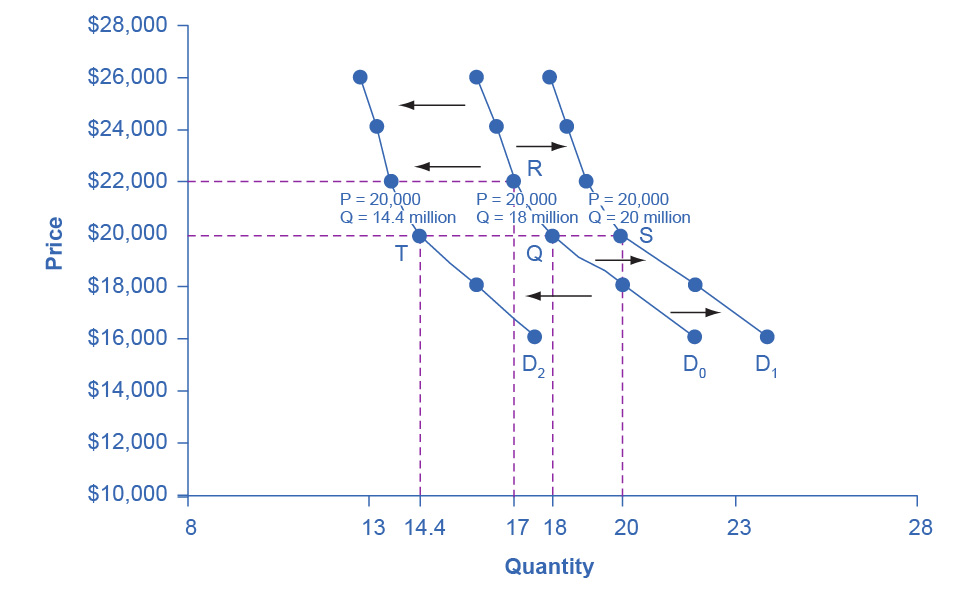
\includegraphics[width=4.88in,height=2.975in]{media/3-2-shifts-in-demand-and-supply-for-goods-and-services_rId33.jpeg}

Figure 3.5 Shifts in Demand: A Car Example Increased demand means that
at every given price, the quantity demanded is higher, so that the
demand curve shifts to the right from D\textsubscript{0} to
D\textsubscript{1}. Decreased demand means that at every given price,
the quantity demanded is lower, so that the demand curve shifts to the
left from D\textsubscript{0} to D\textsubscript{2}.

Table 3.4 Price and Demand Shifts: A Car Example

Now, imagine that the economy slows down so that many people lose their
jobs or work fewer hours, reducing their incomes. In this case, the
decrease in income would lead to a lower quantity of cars demanded at
every given price, and the original demand curve D\textsubscript{0}
would shift left to D\textsubscript{2}. The shift from
D\textsubscript{0} to D\textsubscript{2} represents such a decrease in
demand: At any given price level, the quantity demanded is now lower. In
this example, a price of \$20,000 means 18 million cars sold along the
original demand curve, but only 14.4 million sold after demand fell.

When a demand curve shifts, it does not mean that the quantity demanded
by every individual buyer changes by the same amount. In this example,
not everyone would have higher or lower income and not everyone would
buy or not buy an additional car. Instead, a shift in a demand curve
captures a pattern for the market as a whole.

In the previous section, we argued that higher income causes greater
demand at every price. This is true for most goods and services. For
some---luxury cars, vacations in Europe, and fine jewelry---the effect
of a rise in income can be especially pronounced. A product whose demand
rises when income rises, and vice versa, is called a normal good. A few
exceptions to this pattern do exist. As incomes rise, many people will
buy fewer generic brand groceries and more name brand groceries. They
are less likely to buy used cars and more likely to buy new cars. They
will be less likely to rent an apartment and more likely to own a home.
A product whose demand falls when income rises, and vice versa, is
called an inferior good. In other words, when income increases, the
demand curve shifts to the left.

\hypertarget{other-factors-that-shift-demand-curves}{%
\subsection{Other Factors That Shift Demand
Curves}\label{other-factors-that-shift-demand-curves}}

Income is not the only factor that causes a shift in demand. Other
factors that change demand include tastes and preferences, the
composition or size of the population, the prices of related goods, and
even expectations. A change in any one of the underlying factors that
determine what quantity people are willing to buy at a given price will
cause a shift in demand. Graphically, the new demand curve lies either
to the right (an increase) or to the left (a decrease) of the original
demand curve. Let's look at these factors.

\textbf{Changing Tastes or Preferences}

From 1980 to 2021, the per-person consumption of chicken by Americans
rose from 47 pounds per year to 97 pounds per year, and consumption of
beef fell from 76 pounds per year to 59 pounds per year, according to
the U.S. Department of Agriculture (USDA). Changes like these are
largely due to movements in taste, which change the quantity of a good
demanded at every price: that is, they shift the demand curve for that
good, rightward for chicken and leftward for beef.

\textbf{Changes in the Composition of the Population}

The proportion of elderly citizens in the United States population is
rising. It rose from 9.8\% in 1970 to 12.6\% in 2000, and will be a
projected (by the U.S. Census Bureau) 20\% of the population by 2030. A
society with relatively more children, like the United States in the
1960s, will have greater demand for goods and services like tricycles
and day care facilities. A society with relatively more elderly persons,
as the United States is projected to have by 2030, has a higher demand
for nursing homes and hearing aids. Similarly, changes in the size of
the population can affect the demand for housing and many other goods.
Each of these changes in demand will be shown as a shift in the demand
curve.

\textbf{Changes in the Prices of Related Goods}

Changes in the prices of related goods such as substitutes or
complements also can affect the demand for a product. A substitute is a
good or service that we can use in place of another good or service. As
electronic books, like this one, become more available, you would expect
to see a decrease in demand for traditional printed books. A lower price
for a substitute decreases demand for the other product. For example, in
recent years as the price of tablet computers has fallen, the quantity
demanded has increased (because of the law of demand). Since people are
purchasing tablets, there has been a decrease in demand for laptops,
which we can show graphically as a leftward shift in the demand curve
for laptops. A higher price for a substitute good has the reverse
effect.

Other goods are complements for each other, meaning we often use the
goods together, because consumption of one good tends to enhance
consumption of the other. Examples include breakfast cereal and milk;
notebooks and pens or pencils, golf balls and golf clubs; gasoline and
sport utility vehicles; and the five-way combination of bacon, lettuce,
tomato, mayonnaise, and bread. If the price of golf clubs rises, since
the quantity demanded of golf clubs falls (because of the law of
demand), demand for a complement good like golf balls decreases, too.
Similarly, a higher price for skis would shift the demand curve for a
complement good like ski resort trips to the left, while a lower price
for a complement has the reverse effect.

\textbf{Changes in Expectations about Future Prices or Other Factors
that Affect Demand}

While it is clear that the price of a good affects the quantity
demanded, it is also true that expectations about the future price (or
expectations about tastes and preferences, income, and so on) can affect
demand. For example, if people hear that a hurricane is coming, they may
rush to the store to buy flashlight batteries and bottled water. If
people learn that the price of a good like coffee is likely to rise in
the future, they may head for the store to stock up on coffee now. We
show these changes in demand as shifts in the curve. Therefore, a shift
in demand happens when a change in some economic factor (other than
price) causes a different quantity to be demanded at every price. The
following Work It Out feature shows how this happens.

\hypertarget{work-it-out}{%
\subsection{Work It Out}\label{work-it-out}}

\hypertarget{shift-in-demand}{%
\subsubsection{Shift in Demand}\label{shift-in-demand}}

A shift in demand means that at any price (and at every price), the
quantity demanded will be different than it was before. Following is an
example of a shift in demand due to an income increase.

Step 1. Draw the graph of a demand curve for a normal good like pizza.
Pick a price (like P\textsubscript{0}). Identify the corresponding
Q\textsubscript{0}. See an example in
\protect\hyperlink{CNX_Econ_C03_019}{Figure 3.6}.

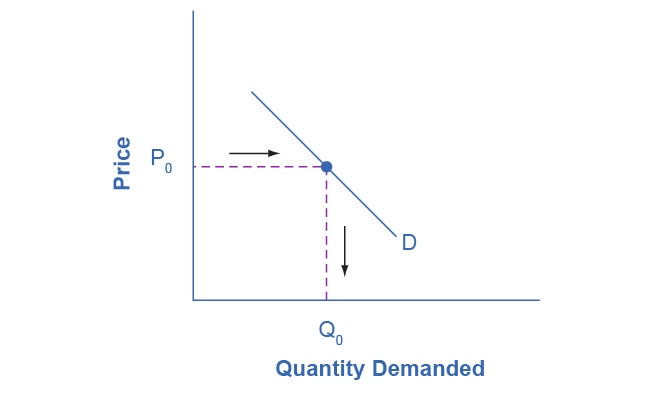
\includegraphics[width=3.25in,height=1.975in]{media/3-2-shifts-in-demand-and-supply-for-goods-and-services_rId44.jpeg}

Figure 3.6 Demand Curve We can use the demand curve to identify how much
consumers would buy at any given price.

Step 2. Suppose income increases. As a result of the change, are
consumers going to buy more or less pizza? The answer is more. Draw a
dotted horizontal line from the chosen price, through the original
quantity demanded, to the new point with the new Q\textsubscript{1}.
Draw a dotted vertical line down to the horizontal axis and label the
new Q\textsubscript{1}. \protect\hyperlink{CNX_Econ_C03_020}{Figure 3.7}
provides an example.

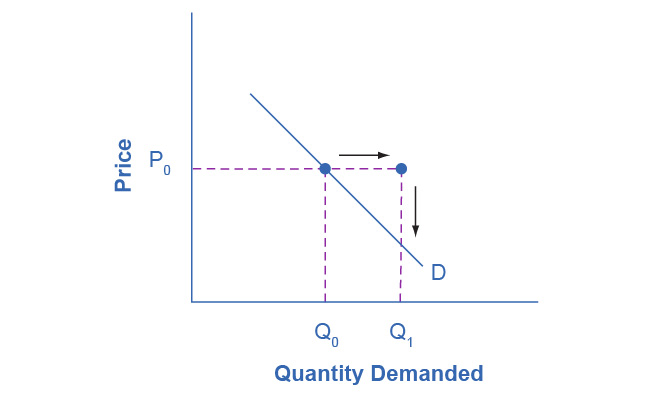
\includegraphics[width=3.25in,height=2.01in]{media/3-2-shifts-in-demand-and-supply-for-goods-and-services_rId47.jpeg}

Figure 3.7 Demand Curve with Income Increase With an increase in income,
consumers will purchase larger quantities, pushing demand to the right.

Step 3. Now, shift the curve through the new point. You will see that an
increase in income causes an upward (or rightward) shift in the demand
curve, so that at any price the quantities demanded will be higher, as
\protect\hyperlink{CNX_Econ_C03_021}{Figure 3.8} illustrates.

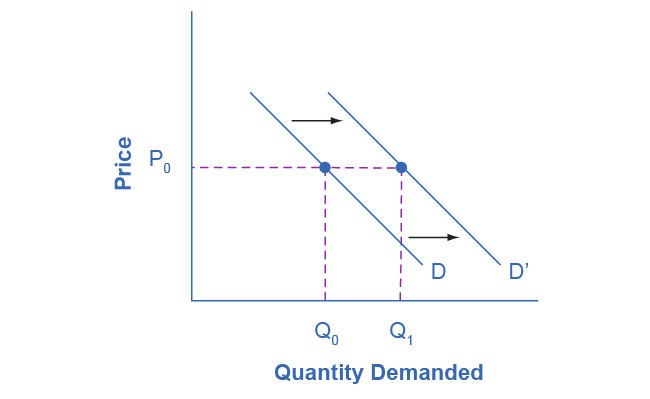
\includegraphics[width=3.25in,height=1.995in]{media/3-2-shifts-in-demand-and-supply-for-goods-and-services_rId50.jpeg}

Figure 3.8 Demand Curve Shifted Right With an increase in income,
consumers will purchase larger quantities, pushing demand to the right,
and causing the demand curve to shift right.

\hypertarget{summing-up-factors-that-change-demand}{%
\subsection{Summing Up Factors That Change
Demand}\label{summing-up-factors-that-change-demand}}

\protect\hyperlink{CNX_Econ_C03_026}{Figure 3.9} summarizes six factors
that can shift demand curves. The direction of the arrows indicates
whether the demand curve shifts represent an increase in demand or a
decrease in demand. Notice that a change in the price of the good or
service itself is not listed among the factors that can shift a demand
curve. A change in the price of a good or service causes a movement
along a specific demand curve, and it typically leads to some change in
the quantity demanded, but it does not shift the demand curve.

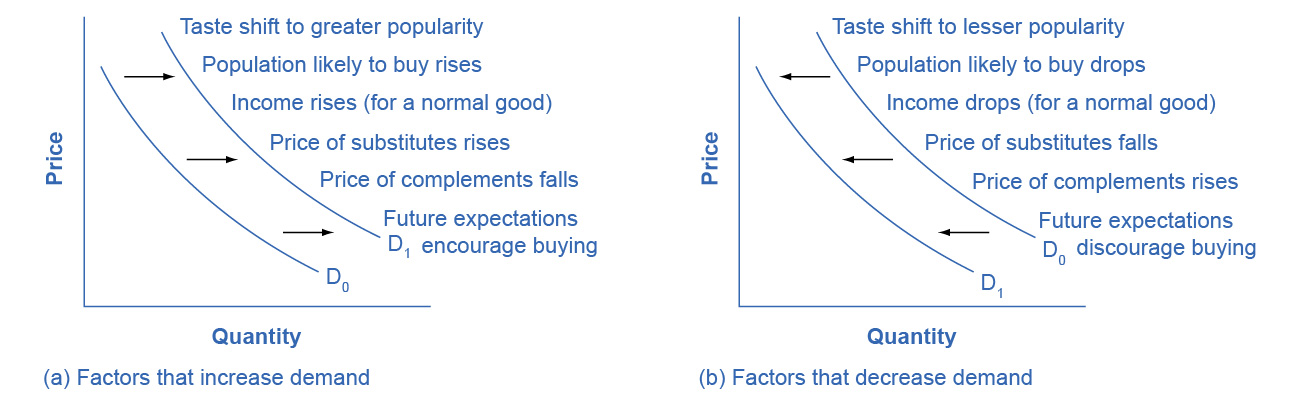
\includegraphics[width=6.5in,height=2.035in]{media/3-2-shifts-in-demand-and-supply-for-goods-and-services_rId56.jpeg}

Figure 3.9 Factors That Shift Demand Curves (a) A list of factors that
can cause an increase in demand from D\textsubscript{0} to
D\textsubscript{1}. (b) The same factors, if their direction is
reversed, can cause a decrease in demand from D\textsubscript{0} to
D\textsubscript{1}.

When a demand curve shifts, it will then intersect with a given supply
curve at a different equilibrium price and quantity. We are, however,
getting ahead of our story. Before discussing how changes in demand can
affect equilibrium price and quantity, we first need to discuss shifts
in supply curves.

\hypertarget{how-production-costs-affect-supply}{%
\subsection{How Production Costs Affect
Supply}\label{how-production-costs-affect-supply}}

A supply curve shows how quantity supplied will change as the price
rises and falls, assuming \emph{ceteris paribus} so that no other
economically relevant factors are changing. If other factors relevant to
supply do change, then the entire supply curve will shift. Just as we
described a shift in demand as a change in the quantity demanded at
every price, a shift in supply means a change in the quantity supplied
at every price.

In thinking about the factors that affect supply, remember what
motivates firms: profits, which are the difference between revenues and
costs. A firm produces goods and services using combinations of labor,
materials, and machinery, or what we call inputs or factors of
production. If a firm faces lower costs of production, while the prices
for the good or service the firm produces remain unchanged, a firm's
profits go up. When a firm's profits increase, it is more motivated to
produce output, since the more it produces the more profit it will earn.
When costs of production fall, a firm will tend to supply a larger
quantity at any given price for its output. We can show this by the
supply curve shifting to the right.

Take, for example, a messenger company that delivers packages around a
city. The company may find that buying gasoline is one of its main
costs. If the price of gasoline falls, then the company will find it can
deliver messages more cheaply than before. Since lower costs correspond
to higher profits, the messenger company may now supply more of its
services at any given price. For example, given the lower gasoline
prices, the company can now serve a greater area, and increase its
supply.

Conversely, if a firm faces higher costs of production, then it will
earn lower profits at any given selling price for its products. As a
result, a higher cost of production typically causes a firm to supply a
smaller quantity at any given price. In this case, the supply curve
shifts to the left.

Consider the supply for cars, shown by curve S\textsubscript{0} in
\protect\hyperlink{CNX_Econ_C03_007}{Figure 3.10}. Point J indicates
that if the price is \$20,000, the quantity supplied will be 18 million
cars. If the price rises to \$22,000 per car, \emph{ceteris paribus,}
the quantity supplied will rise to 20 million cars, as point K on the
S\textsubscript{0} curve shows. We can show the same information in
table form, as in \protect\hyperlink{Table_03_05}{Table 3.5}.

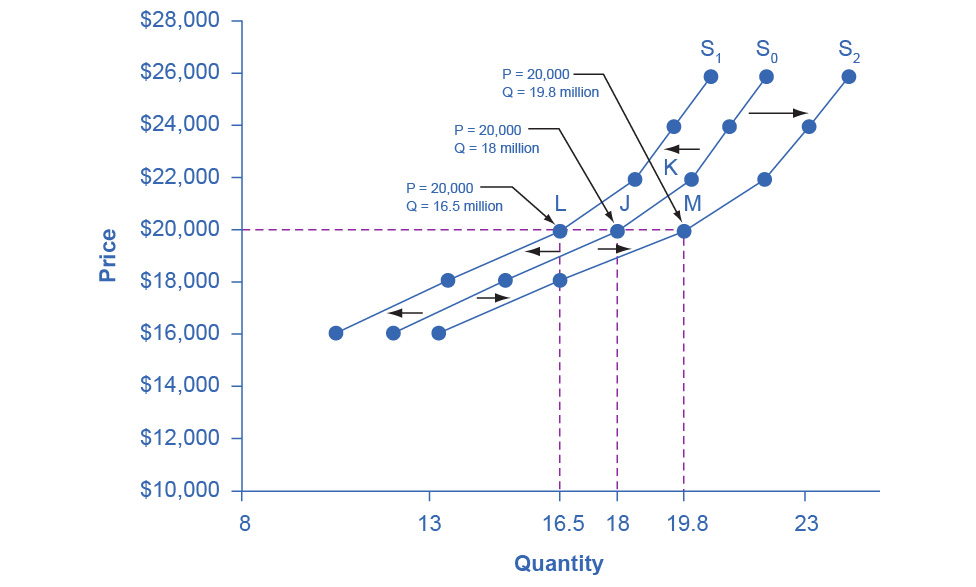
\includegraphics[width=4.88in,height=2.935in]{media/3-2-shifts-in-demand-and-supply-for-goods-and-services_rId64.jpeg}

Figure 3.10 Shifts in Supply: A Car Example Decreased supply means that
at every given price, the quantity supplied is lower, so that the supply
curve shifts to the left, from S\textsubscript{0} to S\textsubscript{1}.
Increased supply means that at every given price, the quantity supplied
is higher, so that the supply curve shifts to the right, from
S\textsubscript{0} to S\textsubscript{2}.

Table 3.5 Price and Shifts in Supply: A Car Example

Now, imagine that the price of steel, an important ingredient in
manufacturing cars, rises, so that producing a car has become more
expensive. At any given price for selling cars, car manufacturers will
react by supplying a lower quantity. We can show this graphically as a
leftward shift of supply, from S\textsubscript{0} to S\textsubscript{1},
which indicates that at any given price, the quantity supplied
decreases. In this example, at a price of \$20,000, the quantity
supplied decreases from 18 million on the original supply curve
(S\textsubscript{0}) to 16.5 million on the supply curve
S\textsubscript{1}, which is labeled as point L.

Conversely, if the price of steel decreases, producing a car becomes
less expensive. At any given price for selling cars, car manufacturers
can now expect to earn higher profits, so they will supply a higher
quantity. The shift of supply to the right, from S\textsubscript{0} to
S\textsubscript{2}, means that at all prices, the quantity supplied has
increased. In this example, at a price of \$20,000, the quantity
supplied increases from 18 million on the original supply curve
(S\textsubscript{0}) to 19.8 million on the supply curve
S\textsubscript{2}, which is labeled M.

\hypertarget{other-factors-that-affect-supply}{%
\subsection{Other Factors That Affect
Supply}\label{other-factors-that-affect-supply}}

In the example above, we saw that changes in the prices of inputs in the
production process will affect the cost of production and thus the
supply. Several other things affect the cost of production, too, such as
changes in weather or other natural conditions, new technologies for
production, and some government policies.

Changes in weather and climate will affect the cost of production for
many agricultural products. For example, in 2014 the Manchurian Plain in
Northeastern China, which produces most of the country\textquotesingle s
wheat, corn, and soybeans, experienced its most severe drought in 50
years. A drought decreases the supply of agricultural products, which
means that at any given price, a lower quantity will be supplied.
Conversely, especially good weather would shift the supply curve to the
right.

When a firm discovers a new technology that allows the firm to produce
at a lower cost, the supply curve will shift to the right, as well. For
instance, in the 1960s a major scientific effort nicknamed the Green
Revolution focused on breeding improved seeds for basic crops like wheat
and rice. By the early 1990s, more than two-thirds of the wheat and rice
in low-income countries around the world used these Green Revolution
seeds---and the harvest was twice as high per acre. A technological
improvement that reduces costs of production will shift supply to the
right, so that a greater quantity will be produced at any given price.

Government policies can affect the cost of production and the supply
curve through taxes, regulations, and subsidies. For example, the U.S.
government imposes a tax on alcoholic beverages that collects about \$8
billion per year from producers. Businesses treat taxes as costs. Higher
costs decrease supply for the reasons we discussed above. Other examples
of policy that can affect cost are the wide array of government
regulations that require firms to spend money to provide a cleaner
environment or a safer workplace. Complying with regulations increases
costs.

A government subsidy, on the other hand, is the opposite of a tax. A
subsidy occurs when the government pays a firm directly or reduces the
firm's taxes if the firm carries out certain actions. From the firm's
perspective, taxes or regulations are an additional cost of production
that shifts supply to the left, leading the firm to produce a lower
quantity at every given price. Government subsidies reduce the cost of
production and increase supply at every given price, shifting supply to
the right. The following Work It Out feature shows how this shift
happens.

\hypertarget{work-it-out-1}{%
\subsection{Work It Out}\label{work-it-out-1}}

\hypertarget{shift-in-supply}{%
\subsubsection{Shift in Supply}\label{shift-in-supply}}

We know that a supply curve shows the minimum price a firm will accept
to produce a given quantity of output. What happens to the supply curve
when the cost of production goes up? Following is an example of a shift
in supply due to a production cost increase. (We'll introduce some other
concepts regarding firm decision-making in Chapters 7 and 8.)

Step 1. Draw a graph of a supply curve for pizza. Pick a quantity (like
Q\textsubscript{0}). If you draw a vertical line up from
Q\textsubscript{0} to the supply curve, you will see the price the firm
chooses. \protect\hyperlink{CNX_Econ_C03_022}{Figure 3.11} provides an
example.

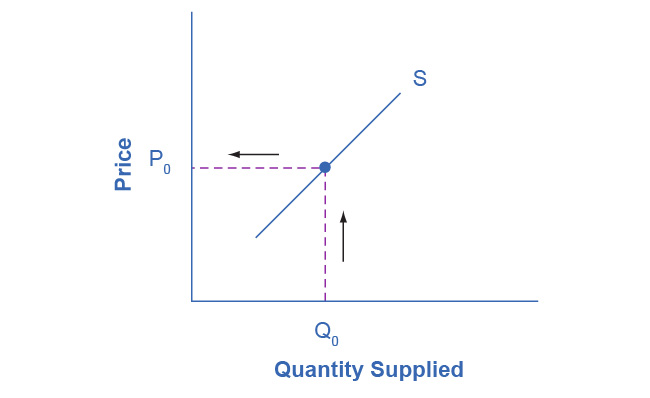
\includegraphics[width=3.25in,height=1.99in]{media/3-2-shifts-in-demand-and-supply-for-goods-and-services_rId70.jpeg}

Figure 3.11 Supply Curve You can use a supply curve to show the minimum
price a firm will accept to produce a given quantity of output.

Step 2. Why did the firm choose that price and not some other? One way
to think about this is that the price is composed of two parts. The
first part is the cost of producing pizzas at the margin; in this case,
the cost of producing the pizza, including cost of ingredients (e.g.,
dough, sauce, cheese, and pepperoni), the cost of the pizza oven, the
shop rent, and the workers\textquotesingle{} wages. The second part is
the firm's desired profit, which is determined, among other factors, by
the profit margins in that particular business. (Desired profit is not
necessarily the same as economic profit, which will be explained in
Chapter 7.) If you add these two parts together, you get the price the
firm wishes to charge. The quantity Q0 and associated price P0 give you
one point on the firm's supply curve, as
\protect\hyperlink{CNX_Econ_C03_023}{Figure 3.12} illustrates.

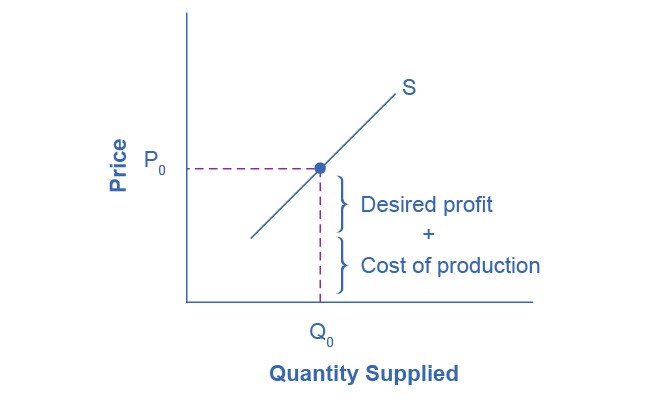
\includegraphics[width=3.25in,height=2.005in]{media/3-2-shifts-in-demand-and-supply-for-goods-and-services_rId73.jpeg}

Figure 3.12 Setting Prices The cost of production and the desired profit
equal the price a firm will set for a product.

Step 3. Now, suppose that the cost of production increases. Perhaps
cheese has become more expensive by \$0.75 per pizza. If that is true,
the firm will want to raise its price by the amount of the increase in
cost (\$0.75). Draw this point on the supply curve directly above the
initial point on the curve, but \$0.75 higher, as
\protect\hyperlink{CNX_Econ_C03_024}{Figure 3.13} shows.

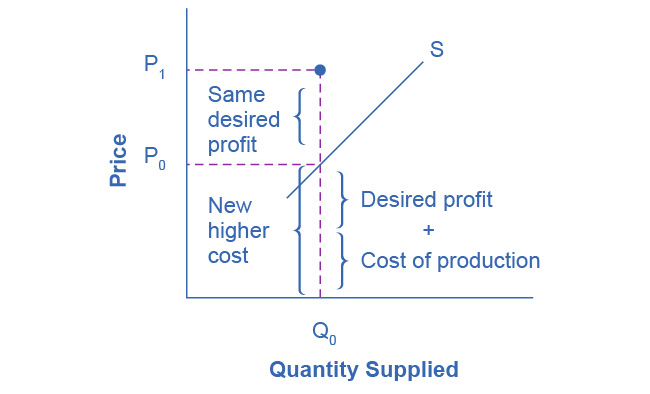
\includegraphics[width=3.25in,height=1.97in]{media/3-2-shifts-in-demand-and-supply-for-goods-and-services_rId76.jpeg}

Figure 3.13 Increasing Costs Leads to Increasing Price Because the cost
of production and the desired profit equal the price a firm will set for
a product, if the cost of production increases, the price for the
product will also need to increase.

Step 4. Shift the supply curve through this point. You will see that an
increase in cost causes an upward (or a leftward) shift of the supply
curve so that at any price, the quantities supplied will be smaller, as
\protect\hyperlink{CNX_Econ_C03_025}{Figure 3.14} illustrates.

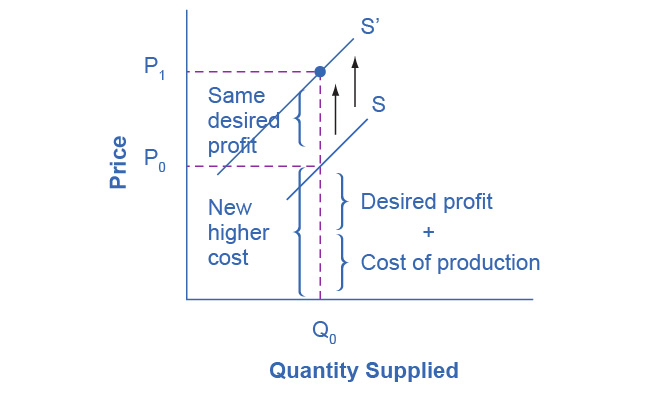
\includegraphics[width=3.25in,height=1.985in]{media/3-2-shifts-in-demand-and-supply-for-goods-and-services_rId79.jpeg}

Figure 3.14 Supply Curve Shifts When the cost of production increases,
the supply curve shifts upwardly to a new price level.

\hypertarget{summing-up-factors-that-change-supply}{%
\subsection{Summing Up Factors That Change
Supply}\label{summing-up-factors-that-change-supply}}

Changes in the cost of inputs, natural disasters, new technologies, and
the impact of government decisions all affect the cost of production. In
turn, these factors affect how much firms are willing to supply at any
given price.

\protect\hyperlink{CNX_Econ_C03_027}{Figure 3.15} summarizes factors
that change the supply of goods and services. Notice that a change in
the price of the product itself is not among the factors that shift the
supply curve. Although a change in price of a good or service typically
causes a change in quantity supplied or a movement along the supply
curve for that specific good or service, it does not cause the supply
curve itself to shift.

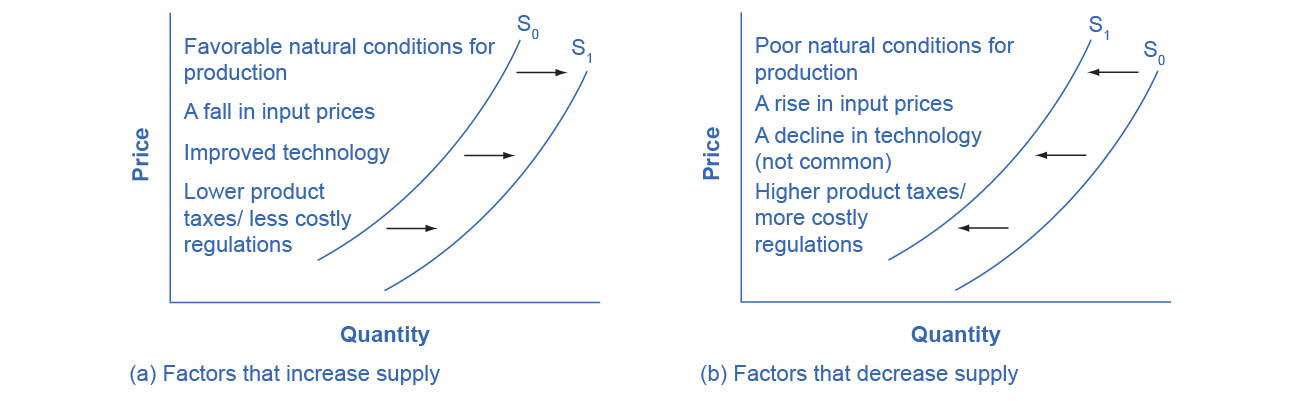
\includegraphics[width=6.5in,height=2.005in]{media/3-2-shifts-in-demand-and-supply-for-goods-and-services_rId85.jpeg}

Figure 3.15 Factors That Shift Supply Curves (a) A list of factors that
can cause an increase in supply from S\textsubscript{0} to
S\textsubscript{1}. (b) The same factors, if their direction is
reversed, can cause a decrease in supply from S\textsubscript{0} to
S\textsubscript{1}.

Because demand and supply curves appear on a two-dimensional diagram
with only price and quantity on the axes, an unwary visitor to the land
of economics might be fooled into believing that economics is about only
four topics: demand, supply, price, and quantity. However, demand and
supply are really ``umbrella'' concepts: demand covers all the factors
that affect demand, and supply covers all the factors that affect
supply. We include factors other than price that affect demand and
supply by using shifts in the demand or the supply curve. In this way,
the two-dimensional demand and supply model becomes a powerful tool for
analyzing a wide range of economic circumstances.

\hypertarget{changes-in-equilibrium-price-and-quantity-the-four-step-process}{%
\chapter{3.3 Changes in Equilibrium Price and Quantity: The Four-Step
Process}\label{changes-in-equilibrium-price-and-quantity-the-four-step-process}}

\hypertarget{learning-objectives-9}{%
\subsection{Learning Objectives}\label{learning-objectives-9}}

By the end of this section, you will be able to:

\begin{itemize}
\tightlist
\item
  Identify equilibrium price and quantity through the four-step process
\item
  Graph equilibrium price and quantity
\item
  Contrast shifts of demand or supply and movements along a demand or
  supply curve
\item
  Graph demand and supply curves, including equilibrium price and
  quantity, based on real-world examples
\end{itemize}

Let's begin this discussion with a single economic event. It might be an
event that affects demand, like a change in income, population, tastes,
prices of substitutes or complements, or expectations about future
prices. It might be an event that affects supply, like a change in
natural conditions, input prices, or technology, or government policies
that affect production. How does this economic event affect equilibrium
price and quantity? We will analyze this question using a four-step
process.

Step 1. Draw a demand and supply model before the economic change took
place. To establish the model requires four standard pieces of
information: The law of demand, which tells us the slope of the demand
curve is negative; the law of supply, which tells us that the slope of
the supply curve is positive; the shift variables for demand; and the
shift variables for supply. From this model, find the initial
equilibrium values for price and quantity.

Step 2. Decide whether the economic change you are analyzing affects
demand or supply. In other words, does the event refer to something in
the list of demand factors or supply factors?

Step 3. Decide whether the effect on demand or supply causes the curve
to shift to the right or to the left, and sketch the new demand or
supply curve on the diagram. In other words, does the event increase or
decrease the amount consumers want to buy or producers want to sell?

Step 4. Identify the new equilibrium and then compare the original
equilibrium price and quantity to the new equilibrium price and
quantity.

Let's consider one example that involves a shift in supply and one that
involves a shift in demand. Then we will consider an example where both
supply and demand shift.

\hypertarget{good-weather-for-salmon-fishing}{%
\subsection{Good Weather for Salmon
Fishing}\label{good-weather-for-salmon-fishing}}

Suppose that during the summer of 2015, weather conditions were
excellent for commercial salmon fishing off the California coast. Heavy
rains meant higher than normal levels of water in the rivers, which
helps the salmon to breed. Slightly cooler ocean temperatures stimulated
the growth of plankton, the microscopic organisms at the bottom of the
ocean food chain, providing everything in the ocean with a hearty food
supply. The ocean stayed calm during fishing season, so commercial
fishing operations did not lose many days to bad weather. How did these
climate conditions affect the quantity and price of salmon?
\protect\hyperlink{CNX_Econ_C03_010}{Figure 3.16} illustrates the
four-step approach, which we explain below, to work through this
problem. \protect\hyperlink{Table_03_07}{Table 3.6} also provides the
information to work the problem.

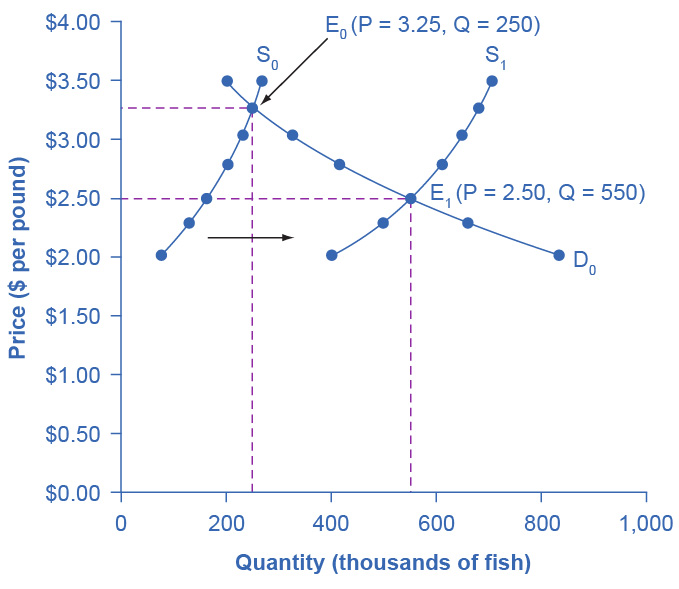
\includegraphics[width=3.395in,height=2.945in]{media/3-3-changes-in-equilibrium-price-and-quantity-the-four-step-process_rId22.jpeg}

Figure 3.16 Good Weather for Salmon Fishing: The Four-Step Process
Unusually good weather leads to changes in the price and quantity of
salmon.

Table 3.6 Salmon Fishing

Step 1. Draw a demand and supply model to illustrate the market for
salmon in the year before the good weather conditions began. The demand
curve D\textsubscript{0} and the supply curve S\textsubscript{0} show
that the original equilibrium price is \$3.25 per pound and the original
equilibrium quantity is 250,000 fish. (This price per pound is what
commercial buyers pay at the fishing docks. What consumers pay at the
grocery is higher.)

Step 2. Did the economic event affect supply or demand? Good weather is
an example of a natural condition that affects supply.

Step 3. Was the effect on supply an increase or a decrease? Good weather
is a change in natural conditions that increases the quantity supplied
at any given price. The supply curve shifts to the right, moving from
the original supply curve S\textsubscript{0} to the new supply curve
S\textsubscript{1}, which \protect\hyperlink{CNX_Econ_C03_010}{Figure
3.16} and \protect\hyperlink{Table_03_07}{Table 3.6} show.

Step 4. Compare the new equilibrium price and quantity to the original
equilibrium. At the new equilibrium E\textsubscript{1}, the equilibrium
price falls from \$3.25 to \$2.50, but the equilibrium quantity
increases from 250,000 to 550,000 salmon. Notice that the equilibrium
quantity demanded increased, even though the demand curve did not move.

In short, good weather conditions increased supply of the California
commercial salmon. The result was a higher equilibrium quantity of
salmon bought and sold in the market at a lower price.

\hypertarget{newspapers-and-the-internet}{%
\subsection{Newspapers and the
Internet}\label{newspapers-and-the-internet}}

According to the Pew Research Center for People and the Press,
increasingly more people, especially younger people, are obtaining their
news from online and digital sources. The majority of U.S. adults now
own smartphones or tablets, and most of those Americans say they use
them in part to access the news. From 2004 to 2012, the share of
Americans who reported obtaining their news from digital sources
increased from 24\% to 39\%. How has this affected consumption of print
news media, and radio and television news?
\protect\hyperlink{CNX_Econ_C03_011}{Figure 3.17} and the text below
illustrates using the four-step analysis to answer this question.

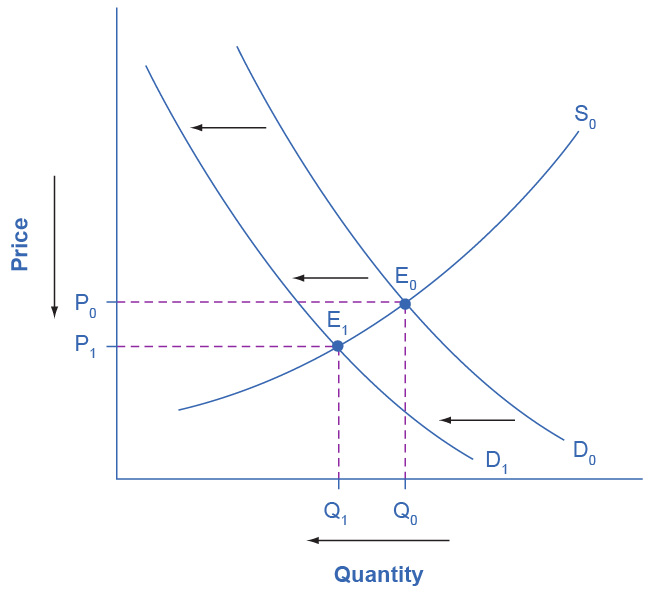
\includegraphics[width=3.255in,height=2.985in]{media/3-3-changes-in-equilibrium-price-and-quantity-the-four-step-process_rId28.jpeg}

Figure 3.17 The Print News Market: A Four-Step Analysis A change in
tastes from print news sources to digital sources results in a leftward
shift in demand for the former. The result is a decrease in both
equilibrium price and quantity.

Step 1. Develop a demand and supply model to think about what the market
looked like before the event. The demand curve D\textsubscript{0} and
the supply curve S\textsubscript{0} show the original relationships. In
this case, we perform the analysis without specific numbers on the price
and quantity axis.

Step 2. Did the described change affect supply or demand? A change in
tastes, from traditional news sources (print, radio, and television) to
digital sources, caused a change in demand for the former.

Step 3. Was the effect on demand positive or negative? A shift to
digital news sources will tend to mean a lower quantity demanded of
traditional news sources at every given price, causing the demand curve
for print and other traditional news sources to shift to the left, from
D\textsubscript{0} to D\textsubscript{1}.

Step 4. Compare the new equilibrium price and quantity to the original
equilibrium price. The new equilibrium (E\textsubscript{1}) occurs at a
lower quantity and a lower price than the original equilibrium
(E\textsubscript{0}).

The decline in print news reading predates 2004. Print newspaper
circulation peaked in 1973 and has declined since then due to
competition from television and radio news. In 1991, 55\% of Americans
indicated they received their news from print sources, while only 29\%
did so in 2012. Radio news has followed a similar path in recent
decades, with the share of Americans obtaining their news from radio
declining from 54\% in 1991 to 33\% in 2012. Television news has held
its own in recent years, with a market share staying in the mid to upper
fifties. What does this suggest for the future, given that two-thirds of
Americans under 30 years old say they do not obtain their news from
television at all?

\hypertarget{the-interconnections-and-speed-of-adjustment-in-real-markets}{%
\subsection{The Interconnections and Speed of Adjustment in Real
Markets}\label{the-interconnections-and-speed-of-adjustment-in-real-markets}}

In the real world, many factors that affect demand and supply can change
all at once. For example, the demand for cars might increase because of
rising incomes and population, and it might decrease because of rising
gasoline prices (a complementary good). Likewise, the supply of cars
might increase because of innovative new technologies that reduce the
cost of car production, and it might decrease as a result of new
government regulations requiring the installation of costly
pollution-control technology.

Moreover, rising incomes and population or changes in gasoline prices
will affect many markets, not just cars. How can an economist sort out
all these interconnected events? The answer lies in the \emph{ceteris
paribus} assumption. Look at how each economic event affects each
market, one event at a time, holding all else constant. Then combine the
analyses to see the net effect.

\hypertarget{a-combined-example}{%
\subsection{A Combined Example}\label{a-combined-example}}

The U.S. Postal Service is facing difficult challenges. Compensation for
postal workers tends to increase most years due to cost-of-living
increases. At the same time, increasingly more people are using email,
text, and other digital message forms such as Facebook and Twitter to
communicate with friends and others. What does this suggest about the
continued viability of the Postal Service?
\protect\hyperlink{CNX_Econ_C03_029}{Figure 3.18} and the text below
illustrate this using the four-step analysis to answer this question.

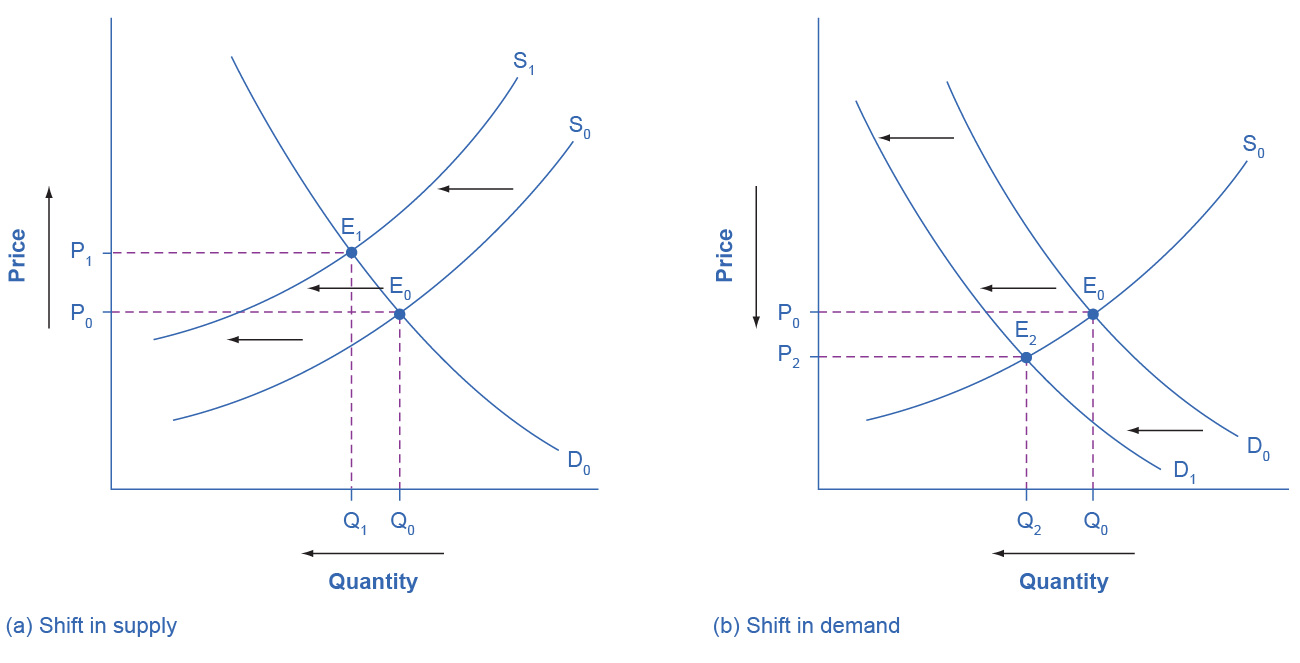
\includegraphics[width=9.72in,height=\textheight]{media/3-3-changes-in-equilibrium-price-and-quantity-the-four-step-process_rId36.jpeg}

\begin{Shaded}
\begin{Highlighting}[]
\ImportTok{import}\NormalTok{ numpy }\ImportTok{as}\NormalTok{ np}
\ImportTok{import}\NormalTok{ matplotlib.pyplot }\ImportTok{as}\NormalTok{ plt}


\CommentTok{\# Generate the graphs for shifts in supply and demand}

\CommentTok{\# Define the original demand and supply curves}
\KeywordTok{def}\NormalTok{ original\_demand(quantity):}
    \ControlFlowTok{return} \FloatTok{2.0} \OperatorTok{{-}} \FloatTok{0.001} \OperatorTok{*}\NormalTok{ quantity}

\KeywordTok{def}\NormalTok{ original\_supply(quantity):}
    \ControlFlowTok{return} \FloatTok{0.5} \OperatorTok{+} \FloatTok{0.001} \OperatorTok{*}\NormalTok{ quantity}

\CommentTok{\# Define the new demand and supply curves after the shift}
\KeywordTok{def}\NormalTok{ new\_demand(quantity):}
    \ControlFlowTok{return} \FloatTok{1.8} \OperatorTok{{-}} \FloatTok{0.001} \OperatorTok{*}\NormalTok{ quantity}

\KeywordTok{def}\NormalTok{ new\_supply(quantity):}
    \ControlFlowTok{return} \FloatTok{0.7} \OperatorTok{+} \FloatTok{0.001} \OperatorTok{*}\NormalTok{ quantity}

\CommentTok{\# Create an array of quantities}
\NormalTok{quantity }\OperatorTok{=}\NormalTok{ np.linspace(}\DecValTok{200}\NormalTok{, }\DecValTok{800}\NormalTok{, }\DecValTok{100}\NormalTok{)}

\CommentTok{\# Generate the corresponding prices for original and new curves}
\NormalTok{original\_demand\_price }\OperatorTok{=}\NormalTok{ original\_demand(quantity)}
\NormalTok{new\_demand\_price }\OperatorTok{=}\NormalTok{ new\_demand(quantity)}
\NormalTok{original\_supply\_price }\OperatorTok{=}\NormalTok{ original\_supply(quantity)}
\NormalTok{new\_supply\_price }\OperatorTok{=}\NormalTok{ new\_supply(quantity)}

\CommentTok{\# Find the equilibrium points for original and new curves}
\NormalTok{original\_equilibrium\_quantity }\OperatorTok{=}\NormalTok{ (}\FloatTok{2.0} \OperatorTok{{-}} \FloatTok{0.5}\NormalTok{) }\OperatorTok{/}\NormalTok{ (}\FloatTok{0.001} \OperatorTok{+} \FloatTok{0.001}\NormalTok{)}
\NormalTok{original\_equilibrium\_price }\OperatorTok{=}\NormalTok{ original\_demand(original\_equilibrium\_quantity)}

\NormalTok{new\_equilibrium\_quantity\_supply }\OperatorTok{=}\NormalTok{ (}\FloatTok{2.0} \OperatorTok{{-}} \FloatTok{0.7}\NormalTok{) }\OperatorTok{/}\NormalTok{ (}\FloatTok{0.001} \OperatorTok{+} \FloatTok{0.001}\NormalTok{)}
\NormalTok{new\_equilibrium\_price\_supply }\OperatorTok{=}\NormalTok{ original\_demand(new\_equilibrium\_quantity\_supply)}

\NormalTok{new\_equilibrium\_quantity\_demand }\OperatorTok{=}\NormalTok{ (}\FloatTok{1.8} \OperatorTok{{-}} \FloatTok{0.5}\NormalTok{) }\OperatorTok{/}\NormalTok{ (}\FloatTok{0.001} \OperatorTok{+} \FloatTok{0.001}\NormalTok{)}
\NormalTok{new\_equilibrium\_price\_demand }\OperatorTok{=}\NormalTok{ new\_demand(new\_equilibrium\_quantity\_demand)}

\CommentTok{\# Create the plots}
\NormalTok{fig, axs }\OperatorTok{=}\NormalTok{ plt.subplots(}\DecValTok{1}\NormalTok{, }\DecValTok{2}\NormalTok{, figsize}\OperatorTok{=}\NormalTok{(}\DecValTok{10}\NormalTok{, }\DecValTok{5}\NormalTok{), sharey}\OperatorTok{=}\VariableTok{True}\NormalTok{)}


\CommentTok{\# Annotate the equilibrium points}
\NormalTok{axs[}\DecValTok{1}\NormalTok{].annotate(}\StringTok{\textquotesingle{}E0\textquotesingle{}}\NormalTok{, }
\NormalTok{                xy}\OperatorTok{=}\NormalTok{(original\_equilibrium\_quantity, original\_equilibrium\_price), }
\NormalTok{                xytext}\OperatorTok{=}\NormalTok{(original\_equilibrium\_quantity }\OperatorTok{+} \DecValTok{10}\NormalTok{, original\_equilibrium\_price }\OperatorTok{{-}} \FloatTok{0.1}\NormalTok{),}
\NormalTok{                arrowprops}\OperatorTok{=}\BuiltInTok{dict}\NormalTok{(facecolor}\OperatorTok{=}\StringTok{\textquotesingle{}black\textquotesingle{}}\NormalTok{, arrowstyle}\OperatorTok{=}\StringTok{\textquotesingle{}{-}\textgreater{}\textquotesingle{}}\NormalTok{))}
\NormalTok{axs[}\DecValTok{1}\NormalTok{].annotate(}\StringTok{\textquotesingle{}E1\textquotesingle{}}\NormalTok{, }
\NormalTok{                xy}\OperatorTok{=}\NormalTok{(new\_equilibrium\_quantity\_demand, new\_equilibrium\_price\_demand), }
\NormalTok{                xytext}\OperatorTok{=}\NormalTok{(new\_equilibrium\_quantity\_demand }\OperatorTok{{-}} \DecValTok{60}\NormalTok{, new\_equilibrium\_price\_demand }\OperatorTok{+} \FloatTok{0.1}\NormalTok{),}
\NormalTok{                arrowprops}\OperatorTok{=}\BuiltInTok{dict}\NormalTok{(facecolor}\OperatorTok{=}\StringTok{\textquotesingle{}black\textquotesingle{}}\NormalTok{, arrowstyle}\OperatorTok{=}\StringTok{\textquotesingle{}{-}\textgreater{}\textquotesingle{}}\NormalTok{))}





\CommentTok{\# Plot for supply shift}
\NormalTok{axs[}\DecValTok{0}\NormalTok{].plot(quantity, original\_demand\_price, label}\OperatorTok{=}\StringTok{\textquotesingle{}D0\textquotesingle{}}\NormalTok{, color}\OperatorTok{=}\StringTok{\textquotesingle{}blue\textquotesingle{}}\NormalTok{)}
\NormalTok{axs[}\DecValTok{0}\NormalTok{].plot(quantity, original\_supply\_price, label}\OperatorTok{=}\StringTok{\textquotesingle{}S0\textquotesingle{}}\NormalTok{, color}\OperatorTok{=}\StringTok{\textquotesingle{}orange\textquotesingle{}}\NormalTok{)}
\NormalTok{axs[}\DecValTok{0}\NormalTok{].plot(quantity, new\_supply\_price, label}\OperatorTok{=}\StringTok{\textquotesingle{}S1\textquotesingle{}}\NormalTok{, color}\OperatorTok{=}\StringTok{\textquotesingle{}orange\textquotesingle{}}\NormalTok{, linestyle}\OperatorTok{=}\StringTok{\textquotesingle{}{-}{-}\textquotesingle{}}\NormalTok{)}
\NormalTok{axs[}\DecValTok{0}\NormalTok{].plot(original\_equilibrium\_quantity, original\_equilibrium\_price, }\StringTok{\textquotesingle{}o\textquotesingle{}}\NormalTok{, color}\OperatorTok{=}\StringTok{\textquotesingle{}green\textquotesingle{}}\NormalTok{)}
\NormalTok{axs[}\DecValTok{0}\NormalTok{].plot(new\_equilibrium\_quantity\_supply, new\_equilibrium\_price\_supply, }\StringTok{\textquotesingle{}o\textquotesingle{}}\NormalTok{, color}\OperatorTok{=}\StringTok{\textquotesingle{}red\textquotesingle{}}\NormalTok{)}
\NormalTok{axs[}\DecValTok{0}\NormalTok{].axhline(y}\OperatorTok{=}\NormalTok{original\_equilibrium\_price, color}\OperatorTok{=}\StringTok{\textquotesingle{}r\textquotesingle{}}\NormalTok{, linestyle}\OperatorTok{=}\StringTok{\textquotesingle{}{-}{-}\textquotesingle{}}\NormalTok{, xmax}\OperatorTok{=}\NormalTok{(original\_equilibrium\_quantity}\OperatorTok{{-}}\DecValTok{200}\NormalTok{)}\OperatorTok{/}\DecValTok{600}\NormalTok{)}
\NormalTok{axs[}\DecValTok{0}\NormalTok{].axvline(x}\OperatorTok{=}\NormalTok{original\_equilibrium\_quantity, color}\OperatorTok{=}\StringTok{\textquotesingle{}r\textquotesingle{}}\NormalTok{, linestyle}\OperatorTok{=}\StringTok{\textquotesingle{}{-}{-}\textquotesingle{}}\NormalTok{, ymax}\OperatorTok{=}\NormalTok{(original\_equilibrium\_price}\OperatorTok{{-}}\FloatTok{0.5}\NormalTok{)}\OperatorTok{/}\FloatTok{1.5}\NormalTok{)}
\NormalTok{axs[}\DecValTok{0}\NormalTok{].axhline(y}\OperatorTok{=}\NormalTok{new\_equilibrium\_price\_supply, color}\OperatorTok{=}\StringTok{\textquotesingle{}r\textquotesingle{}}\NormalTok{, linestyle}\OperatorTok{=}\StringTok{\textquotesingle{}:\textquotesingle{}}\NormalTok{, xmax}\OperatorTok{=}\NormalTok{(new\_equilibrium\_quantity\_supply}\OperatorTok{{-}}\DecValTok{200}\NormalTok{)}\OperatorTok{/}\DecValTok{600}\NormalTok{)}
\NormalTok{axs[}\DecValTok{0}\NormalTok{].axvline(x}\OperatorTok{=}\NormalTok{new\_equilibrium\_quantity\_supply, color}\OperatorTok{=}\StringTok{\textquotesingle{}r\textquotesingle{}}\NormalTok{, linestyle}\OperatorTok{=}\StringTok{\textquotesingle{}:\textquotesingle{}}\NormalTok{, ymax}\OperatorTok{=}\NormalTok{(new\_equilibrium\_price\_supply}\OperatorTok{{-}}\FloatTok{0.5}\NormalTok{)}\OperatorTok{/}\FloatTok{1.5}\NormalTok{)}

\CommentTok{\# Plot for demand shift}
\NormalTok{axs[}\DecValTok{1}\NormalTok{].plot(quantity, original\_demand\_price, label}\OperatorTok{=}\StringTok{\textquotesingle{}D0\textquotesingle{}}\NormalTok{, color}\OperatorTok{=}\StringTok{\textquotesingle{}blue\textquotesingle{}}\NormalTok{, linestyle}\OperatorTok{=}\StringTok{\textquotesingle{}{-}{-}\textquotesingle{}}\NormalTok{)}
\NormalTok{axs[}\DecValTok{1}\NormalTok{].plot(quantity, new\_demand\_price, label}\OperatorTok{=}\StringTok{\textquotesingle{}D1\textquotesingle{}}\NormalTok{, color}\OperatorTok{=}\StringTok{\textquotesingle{}blue\textquotesingle{}}\NormalTok{)}
\NormalTok{axs[}\DecValTok{1}\NormalTok{].plot(quantity, original\_supply\_price, label}\OperatorTok{=}\StringTok{\textquotesingle{}S0\textquotesingle{}}\NormalTok{, color}\OperatorTok{=}\StringTok{\textquotesingle{}orange\textquotesingle{}}\NormalTok{)}
\NormalTok{axs[}\DecValTok{1}\NormalTok{].plot(original\_equilibrium\_quantity, original\_equilibrium\_price, }\StringTok{\textquotesingle{}o\textquotesingle{}}\NormalTok{, color}\OperatorTok{=}\StringTok{\textquotesingle{}green\textquotesingle{}}\NormalTok{)}
\NormalTok{axs[}\DecValTok{1}\NormalTok{].plot(new\_equilibrium\_quantity\_demand, new\_equilibrium\_price\_demand, }\StringTok{\textquotesingle{}o\textquotesingle{}}\NormalTok{, color}\OperatorTok{=}\StringTok{\textquotesingle{}red\textquotesingle{}}\NormalTok{)}
\NormalTok{axs[}\DecValTok{1}\NormalTok{].axhline(y}\OperatorTok{=}\NormalTok{original\_equilibrium\_price, color}\OperatorTok{=}\StringTok{\textquotesingle{}r\textquotesingle{}}\NormalTok{, linestyle}\OperatorTok{=}\StringTok{\textquotesingle{}{-}{-}\textquotesingle{}}\NormalTok{, xmax}\OperatorTok{=}\NormalTok{(original\_equilibrium\_quantity}\OperatorTok{{-}}\DecValTok{200}\NormalTok{)}\OperatorTok{/}\DecValTok{600}\NormalTok{)}
\NormalTok{axs[}\DecValTok{1}\NormalTok{].axvline(x}\OperatorTok{=}\NormalTok{original\_equilibrium\_quantity, color}\OperatorTok{=}\StringTok{\textquotesingle{}r\textquotesingle{}}\NormalTok{, linestyle}\OperatorTok{=}\StringTok{\textquotesingle{}{-}{-}\textquotesingle{}}\NormalTok{, ymax}\OperatorTok{=}\NormalTok{(original\_equilibrium\_price}\OperatorTok{{-}}\FloatTok{0.5}\NormalTok{)}\OperatorTok{/}\FloatTok{1.5}\NormalTok{)}
\NormalTok{axs[}\DecValTok{1}\NormalTok{].axhline(y}\OperatorTok{=}\NormalTok{new\_equilibrium\_price\_demand, color}\OperatorTok{=}\StringTok{\textquotesingle{}r\textquotesingle{}}\NormalTok{, linestyle}\OperatorTok{=}\StringTok{\textquotesingle{}:\textquotesingle{}}\NormalTok{, xmax}\OperatorTok{=}\NormalTok{(new\_equilibrium\_quantity\_demand}\OperatorTok{{-}}\DecValTok{200}\NormalTok{)}\OperatorTok{/}\DecValTok{600}\NormalTok{)}
\NormalTok{axs[}\DecValTok{1}\NormalTok{].axvline(x}\OperatorTok{=}\NormalTok{new\_equilibrium\_quantity\_demand, color}\OperatorTok{=}\StringTok{\textquotesingle{}r\textquotesingle{}}\NormalTok{, linestyle}\OperatorTok{=}\StringTok{\textquotesingle{}:\textquotesingle{}}\NormalTok{, ymax}\OperatorTok{=}\NormalTok{(new\_equilibrium\_price\_demand}\OperatorTok{{-}}\FloatTok{0.5}\NormalTok{)}\OperatorTok{/}\FloatTok{1.5}\NormalTok{)}

\CommentTok{\# Set titles and labels}
\NormalTok{axs[}\DecValTok{0}\NormalTok{].set\_title(}\StringTok{\textquotesingle{}(a) Shift in supply\textquotesingle{}}\NormalTok{)}
\NormalTok{axs[}\DecValTok{1}\NormalTok{].set\_title(}\StringTok{\textquotesingle{}(b) Shift in demand\textquotesingle{}}\NormalTok{)}
\ControlFlowTok{for}\NormalTok{ ax }\KeywordTok{in}\NormalTok{ axs:}
\NormalTok{    ax.set\_xlabel(}\StringTok{\textquotesingle{}Quantity\textquotesingle{}}\NormalTok{)}
\NormalTok{    ax.set\_ylabel(}\StringTok{\textquotesingle{}Price\textquotesingle{}}\NormalTok{)}
\NormalTok{    ax.legend()}

\CommentTok{\# Show the plots}
\NormalTok{plt.tight\_layout()}
\NormalTok{plt.show()}
\end{Highlighting}
\end{Shaded}

\begin{figure}[H]

{\centering 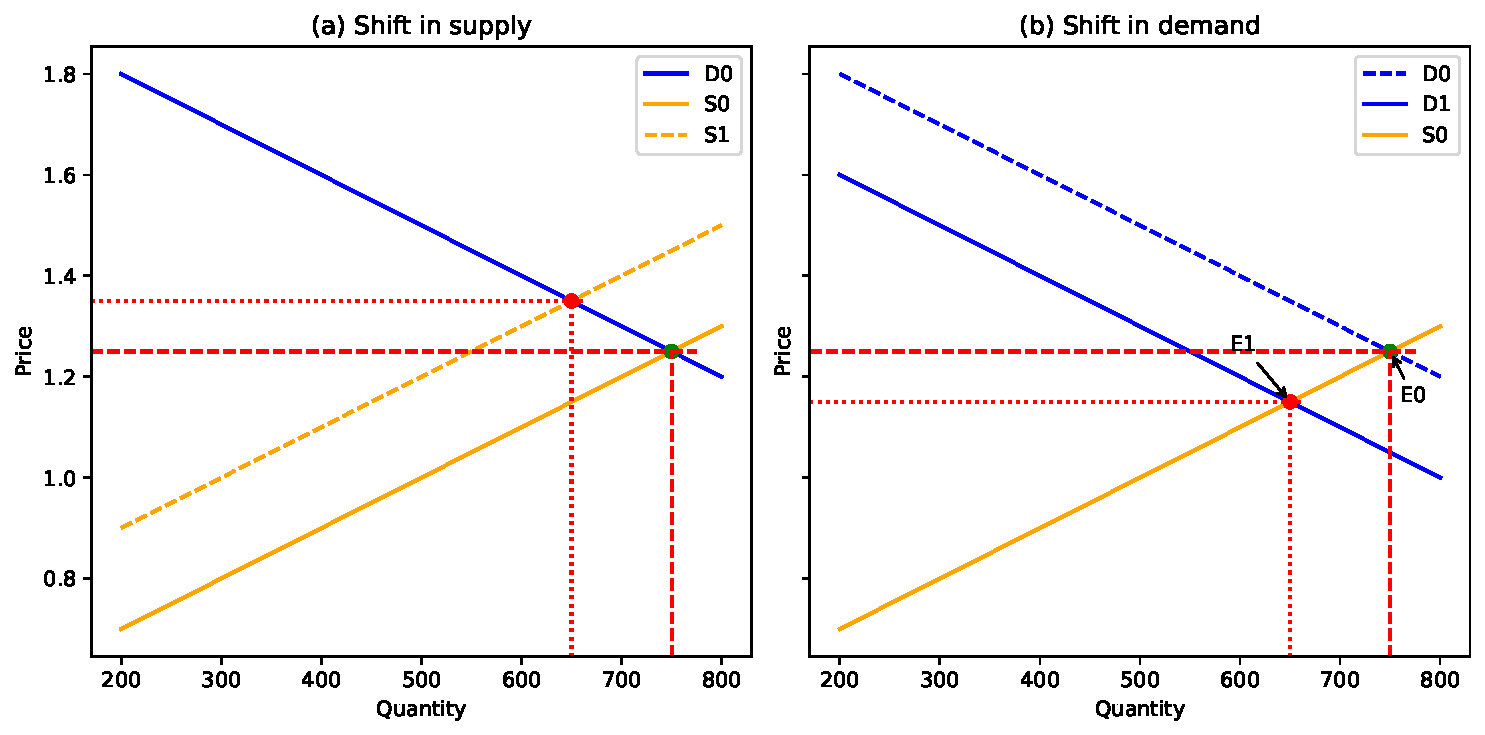
\includegraphics{3-3-changes-in-equilibrium-price-and-quantity-the-four-step-process_files/figure-pdf/cell-2-output-1.pdf}

}

\end{figure}

Figure 3.18 Higher Compensation for Postal Workers: A Four-Step Analysis
(a) Higher labor compensation causes a leftward shift in the supply
curve, a decrease in the equilibrium quantity, and an increase in the
equilibrium price. (b) A change in tastes away from Postal Services
causes a leftward shift in the demand curve, a decrease in the
equilibrium quantity, and a decrease in the equilibrium price.

Since this problem involves two disturbances, we need two four-step
analyses, the first to analyze the effects of higher compensation for
postal workers, the second to analyze the effects of many people
switching from ``snail mail'' to email and other digital messages.

\protect\hyperlink{CNX_Econ_C03_029}{Figure 3.18} (a) shows the shift in
supply discussed in the following steps.

Step 1. Draw a demand and supply model to illustrate what the market for
the U.S. Postal Service looked like before this scenario starts. The
demand curve D\textsubscript{0} and the supply curve S\textsubscript{0}
show the original relationships.

Step 2. Did the described change affect supply or demand? Labor
compensation is a cost of production. A change in production costs
caused a change in supply for the Postal Service.

Step 3. Was the effect on supply positive or negative? Higher labor
compensation leads to a lower quantity supplied of postal services at
every given price, causing the supply curve for postal services to shift
to the left, from S\textsubscript{0} to S\textsubscript{1}.

Step 4. Compare the new equilibrium price and quantity to the original
equilibrium price. The new equilibrium (E\textsubscript{1}) occurs at a
lower quantity and a higher price than the original equilibrium
(E\textsubscript{0}).

\protect\hyperlink{CNX_Econ_C03_029}{Figure 3.18} (b) shows the shift in
demand in the following steps.

Step 1. Draw a demand and supply model to illustrate what the market for
U.S. Postal Services looked like before this scenario starts. The demand
curve D\textsubscript{0} and the supply curve S\textsubscript{0} show
the original relationships. Note that this diagram is independent from
the diagram in panel (a).

Step 2. Did the change described affect supply or demand? A change in
tastes away from snail mail toward digital messages will cause a change
in demand for the Postal Service.

Step 3. Was the effect on demand positive or negative? A change in
tastes away from snailmail toward digital messages causes lower quantity
demanded of postal services at every given price, causing the demand
curve for postal services to shift to the left, from D\textsubscript{0}
to D\textsubscript{1}.

Step 4. Compare the new equilibrium price and quantity to the original
equilibrium price. The new equilibrium (E\textsubscript{2}) occurs at a
lower quantity and a lower price than the original equilibrium
(E\textsubscript{0}).

The final step in a scenario where both supply and demand shift is to
combine the two individual analyses to determine what happens to the
equilibrium quantity and price. Graphically, we superimpose the previous
two diagrams one on top of the other, as in
\protect\hyperlink{CNX_Econ_C03_030}{Figure 3.19}.

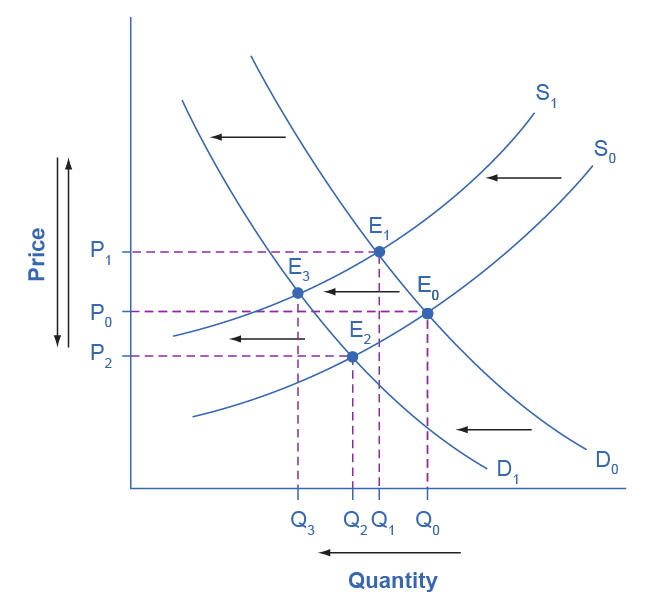
\includegraphics[width=3.255in,height=3.07in]{media/3-3-changes-in-equilibrium-price-and-quantity-the-four-step-process_rId39.jpeg}

Figure 3.19 Combined Effect of Decreased Demand and Decreased Supply
Supply and demand shifts cause changes in equilibrium price and
quantity.

Following are the results:

Effect on Quantity: The effect of higher labor compensation on Postal
Services because it raises the cost of production is to decrease the
equilibrium quantity. The effect of a change in tastes away from snail
mail is to decrease the equilibrium quantity. Since both shifts are to
the left, the overall impact is a decrease in the equilibrium quantity
of Postal Services (Q\textsubscript{3}). This is easy to see
graphically, since Q\textsubscript{3} is to the left of
Q\textsubscript{0}.

Effect on Price: The overall effect on price is more complicated. The
effect of higher labor compensation on Postal Services, because it
raises the cost of production, is to increase the equilibrium price. The
effect of a change in tastes away from snail mail is to decrease the
equilibrium price. Since the two effects are in opposite directions,
unless we know the magnitudes of the two effects, the overall effect is
unclear. This is not unusual. When both curves shift, typically we can
determine the overall effect on price or on quantity, but not on both.
In this case, we determined the overall effect on the equilibrium
quantity, but not on the equilibrium price. In other cases, it might be
the opposite.

The next Clear It Up feature focuses on the difference between shifts of
supply or demand and movements along a curve.

\hypertarget{clear-it-up}{%
\subsection{Clear It Up}\label{clear-it-up}}

\hypertarget{what-is-the-difference-between-shifts-of-demand-or-supply-versus-movements-along-a-demand-or-supply-curve}{%
\subsubsection{What is the difference between shifts of demand or supply
versus movements along a demand or supply
curve?}\label{what-is-the-difference-between-shifts-of-demand-or-supply-versus-movements-along-a-demand-or-supply-curve}}

One common mistake in applying the demand and supply framework is to
confuse the shift of a demand or a supply curve with movement along a
demand or supply curve. As an example, consider a problem that asks
whether a drought will increase or decrease the equilibrium quantity and
equilibrium price of wheat. Lee, a student in an introductory economics
class, might reason:

``Well, it is clear that a drought reduces supply, so I will shift back
the supply curve, as in the shift from the original supply curve
S\textsubscript{0} to S\textsubscript{1} on the diagram (Shift 1). The
equilibrium moves from E\textsubscript{0} to E\textsubscript{1}, the
equilibrium quantity is lower and the equilibrium price is higher. Then,
a higher price makes farmers more likely to supply the good, so the
supply curve shifts right, as shows the shift from S\textsubscript{1} to
S\textsubscript{2}, shows on the diagram (Shift 2), so that the
equilibrium now moves from E\textsubscript{1} to E\textsubscript{2}. The
higher price, however, also reduces demand and so causes demand to shift
back, like the shift from the original demand curve, D\textsubscript{0}
to D\textsubscript{1} on the diagram (labeled Shift 3), and the
equilibrium moves from E\textsubscript{2} to E\textsubscript{3}.''

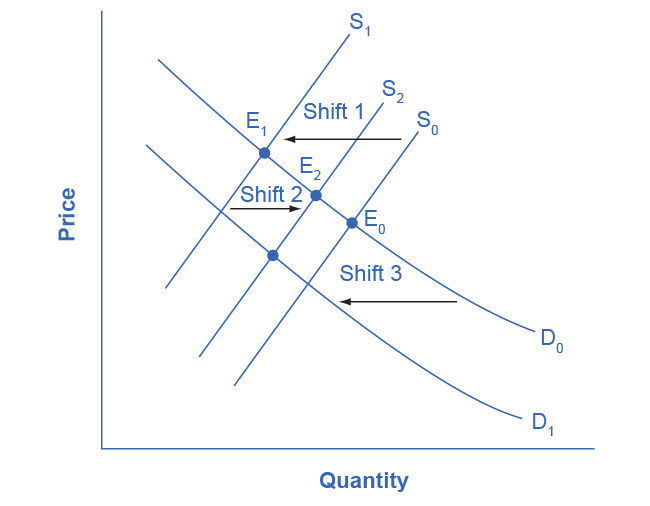
\includegraphics[width=3.25in,height=2.53in]{media/3-3-changes-in-equilibrium-price-and-quantity-the-four-step-process_rId43.jpeg}

Figure 3.20 Shifts of Demand or Supply versus Movements along a Demand
or Supply Curve A shift in one curve never causes a shift in the other
curve. Rather, a shift in one curve causes a movement along the second
curve.

At about this point, Lee suspects that this answer is headed down the
wrong path. Think about what might be wrong with Lee's logic, and then
read the answer that follows.

\emph{Answer:} Lee's first step is correct: that is, a drought shifts
back the supply curve of wheat and leads to a prediction of a lower
equilibrium quantity and a higher equilibrium price. This corresponds to
a movement along the original demand curve (D\textsubscript{0}), from
E\textsubscript{0} to E\textsubscript{1}. The rest of Lee's argument is
wrong, because it mixes up shifts in supply with quantity supplied, and
shifts in demand with quantity demanded. A higher or lower price never
shifts the supply curve, as suggested by the shift in supply from
S\textsubscript{1} to S\textsubscript{2}. Instead, a price change leads
to a movement along a given supply curve. Similarly, a higher or lower
price never shifts a demand curve, as suggested in the shift from
D\textsubscript{0} to D\textsubscript{1}. Instead, a price change leads
to a movement along a given demand curve. Remember, a change in the
price of a good never causes the demand or supply curve for that good to
shift.

Think carefully about the timeline of events: What happens first, what
happens next? What is cause, what is effect? If you keep the order
right, you are more likely to get the analysis correct.

In the four-step analysis of how economic events affect equilibrium
price and quantity, the movement from the old to the new equilibrium
seems immediate. As a practical matter, however, prices and quantities
often do not zoom straight to equilibrium. More realistically, when an
economic event causes demand or supply to shift, prices and quantities
set off in the general direction of equilibrium. Even as they are moving
toward one new equilibrium, a subsequent change in demand or supply
often pushes prices toward another equilibrium.

\hypertarget{price-ceilings-and-price-floors}{%
\chapter{3.4 Price Ceilings and Price
Floors}\label{price-ceilings-and-price-floors}}

\hypertarget{learning-objectives-10}{%
\subsection{Learning Objectives}\label{learning-objectives-10}}

By the end of this section, you will be able to:

\begin{itemize}
\tightlist
\item
  Explain price controls, price ceilings, and price floors
\item
  Analyze demand and supply as a social adjustment mechanism
\end{itemize}

To this point in the chapter, we have been assuming that markets are
free, that is, they operate with no government intervention. In this
section, we will explore the outcomes, both anticipated and otherwise,
when government does intervene in a market either to prevent the price
of some good or service from rising ``too high'' or to prevent the price
of some good or service from falling ``too low''.

Economists believe there are a small number of fundamental principles
that explain how economic agents respond in different situations. Two of
these principles, which we have already introduced, are the laws of
demand and supply.

Governments can pass laws affecting market outcomes, but no law can
negate these economic principles. Rather, the principles will become
apparent in sometimes unexpected ways, which may undermine the intent of
the government policy. This is one of the major conclusions of this
section.

Controversy sometimes surrounds the prices and quantities established by
demand and supply, especially for products that are considered
necessities. In some cases, discontent over prices turns into public
pressure on politicians, who may then pass legislation to prevent a
certain price from climbing ``too high'' or falling ``too low.''

The demand and supply model shows how people and firms will react to the
incentives that these laws provide to control prices, in ways that will
often lead to undesirable consequences. Alternative policy tools can
often achieve the desired goals of price control laws, while avoiding at
least some of their costs and tradeoffs.

\hypertarget{price-ceilings}{%
\subsection{Price Ceilings}\label{price-ceilings}}

Laws that governments enact to regulate prices are called price
controls. Price controls come in two flavors. A price ceiling keeps a
price from rising above a certain level (the ``ceiling''), while a price
floor keeps a price from falling below a given level (the ``floor'').
This section uses the demand and supply framework to analyze price
ceilings. The next section discusses price floors.

A price ceiling is a legal maximum price that one pays for some good or
service. A government imposes price ceilings in order to keep the price
of some necessary good or service affordable. For example, in 2005
during Hurricane Katrina, the price of bottled water increased above \$5
per gallon. As a result, many people called for price controls on
bottled water to prevent the price from rising so high. In this
particular case, the government did not impose a price ceiling, but
there are other examples of where price ceilings did occur.

In many markets for goods and services, demanders outnumber suppliers.
Consumers, who are also potential voters, sometimes unite behind a
political proposal to hold down a certain price. In some cities, such as
Albany, renters have pressed political leaders to pass rent control
laws, a price ceiling that usually works by stating that landlords can
raise rents by only a certain maximum percentage each year. Some of the
best examples of rent control occur in urban areas such as New York,
Washington D.C., or San Francisco.

Rent control becomes a politically hot topic when rents begin to rise
rapidly. Everyone needs an affordable place to live. Perhaps a change in
tastes makes a certain suburb or town a more popular place to live.
Perhaps locally-based businesses expand, bringing higher incomes and
more people into the area. Such changes can cause a change in the demand
for rental housing, as \protect\hyperlink{CNX_Econ_C03_012}{Figure 3.21}
illustrates. The original equilibrium (E\textsubscript{0}) lies at the
intersection of supply curve S\textsubscript{0} and demand curve
D\textsubscript{0}, corresponding to an equilibrium price of \$500 and
an equilibrium quantity of 15,000 units of rental housing. The effect of
greater income or a change in tastes is to shift the demand curve for
rental housing to the right, as the data in
\protect\hyperlink{Table_03_10}{Table 3.7} shows and the shift from
D\textsubscript{0} to D\textsubscript{1} on the graph. In this market,
at the new equilibrium E\textsubscript{1}, the price of a rental unit
would rise to \$600 and the equilibrium quantity would increase to
17,000 units.

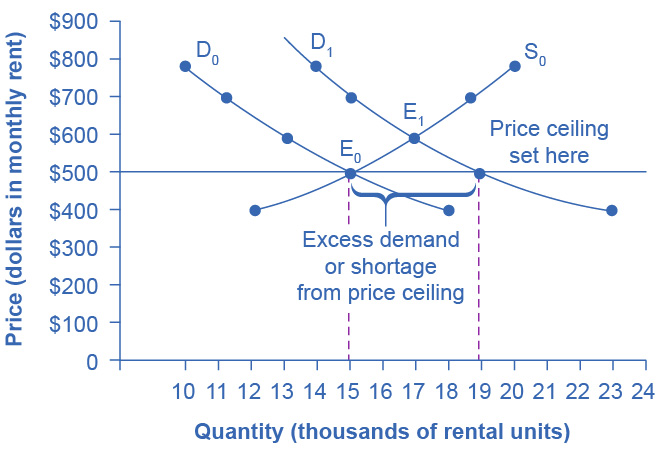
\includegraphics[width=3.29in,height=2.285in]{media/3-4-price-ceilings-and-price-floors_rId25.jpeg}

Figure 3.21 A Price Ceiling Example---Rent Control The original
intersection of demand and supply occurs at E\textsubscript{0}. If
demand shifts from D\textsubscript{0} to D\textsubscript{1}, the new
equilibrium would be at E\textsubscript{1}---unless a price ceiling
prevents the price from rising. If the price is not permitted to rise,
the quantity supplied remains at 15,000. However, after the change in
demand, the quantity demanded rises to 19,000, resulting in a shortage.

Table 3.7 Rent Control

Suppose that a city government passes a rent control law to keep the
price at the original equilibrium of \$500 for a typical apartment. In
\protect\hyperlink{CNX_Econ_C03_012}{Figure 3.21}, the horizontal line
at the price of \$500 shows the legally fixed maximum price set by the
rent control law. However, the underlying forces that shifted the demand
curve to the right are still there. At that price (\$500), the quantity
supplied remains at the same 15,000 rental units, but the quantity
demanded is 19,000 rental units. In other words, the quantity demanded
exceeds the quantity supplied, so there is a shortage of rental housing.
One of the ironies of price ceilings is that while the price ceiling was
intended to help renters, there are actually fewer apartments rented out
under the price ceiling (15,000 rental units) than would be the case at
the market rent of \$600 (17,000 rental units).

Price ceilings do not simply benefit renters at the expense of
landlords. Rather, some renters (or potential renters) lose their
housing as landlords convert apartments to co-ops and condos. Even when
the housing remains in the rental market, landlords tend to spend less
on maintenance and on essentials like heating, cooling, hot water, and
lighting. The first rule of economics is you do not get something for
nothing---everything has an opportunity cost. Thus, if renters obtain
``cheaper'' housing than the market requires, they tend to also end up
with lower quality housing.

Price ceilings are enacted in an attempt to keep prices low for those
who need the product. However, when the market price is not allowed to
rise to the equilibrium level, quantity demanded exceeds quantity
supplied, and thus a shortage occurs. Those who manage to purchase the
product at the lower price given by the price ceiling will benefit, but
sellers of the product will suffer, along with those who are not able to
purchase the product at all. Quality is also likely to deteriorate.

\hypertarget{price-floors}{%
\subsection{Price Floors}\label{price-floors}}

A price floor is the lowest price that one can legally pay for some good
or service. Perhaps the best-known example of a price floor is the
minimum wage, which is based on the view that someone working full time
should be able to afford a basic standard of living. The federal minimum
wage in 2022 was \$7.25 per hour, although some states and localities
have a higher minimum wage. The federal minimum wage yields an annual
income for a single person of \$15,080, which is slightly higher than
the Federal poverty line of \$11,880. Congress periodically raises the
federal minimum wage as the cost of living rises. As of March 2022, the
most recent adjustment occurred in 2009, when the federal minimum wage
was raised from \$6.55 to \$7.25.

Price floors are sometimes called ``price supports,'' because they
support a price by preventing it from falling below a certain level.
Around the world, many countries have passed laws to create agricultural
price supports. Farm prices and thus farm incomes fluctuate, sometimes
widely. Even if, on average, farm incomes are adequate, some years they
can be quite low. The purpose of price supports is to prevent these
swings.

The most common way price supports work is that the government enters
the market and buys up the product, adding to demand to keep prices
higher than they otherwise would be. According to the Common
Agricultural Policy reform effective in 2019, the European Union (EU)
will spend about 58 billion euros per year, or 65.5 billion dollars per
year (with the December 2021 exchange rate), or roughly 36\% of the EU
budget, on price supports for Europe's farmers.

\protect\hyperlink{CNX_Econ_C03_013}{Figure 3.22} illustrates the
effects of a government program that assures a price above the
equilibrium by focusing on the market for wheat in Europe. In the
absence of government intervention, the price would adjust so that the
quantity supplied would equal the quantity demanded at the equilibrium
point E\textsubscript{0}, with price P\textsubscript{0} and quantity
Q\textsubscript{0}. However, policies to keep prices high for farmers
keep the price above what would have been the market equilibrium
level---the price Pf shown by the dashed horizontal line in the diagram.
The result is a quantity supplied in excess of the quantity demanded
(Qd). When quantity supplied exceeds quantity demanded, a surplus
exists.

Economists estimate that the high-income areas of the world, including
the United States, Europe, and Japan, spend roughly \$1 billion per day
in supporting their farmers. If the government is willing to purchase
the excess supply (or to provide payments for others to purchase it),
then farmers will benefit from the price floor, but taxpayers and
consumers of food will pay the costs. Agricultural economists and policy
makers have offered numerous proposals for reducing farm subsidies. In
many countries, however, political support for subsidies for farmers
remains strong. This is either because the population views this as
supporting the traditional rural way of life or because of
industry\textquotesingle s lobbying power of the agro-business.

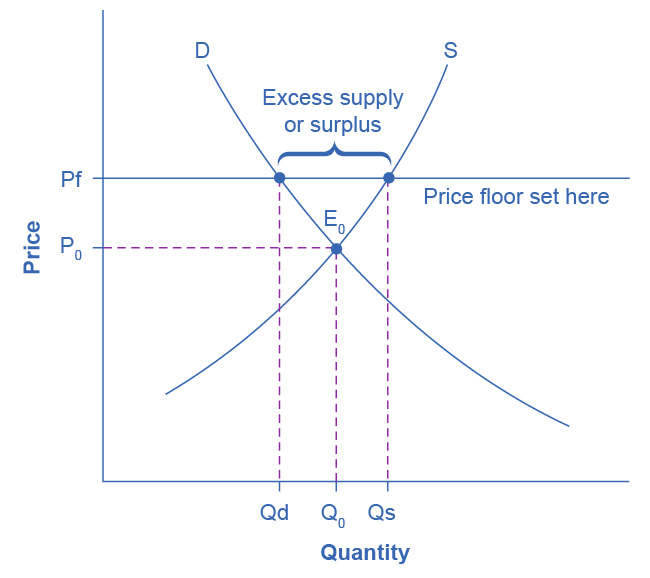
\includegraphics[width=3.25in,height=2.89in]{media/3-4-price-ceilings-and-price-floors_rId31.jpeg}

Figure 3.22 European Wheat Prices: A Price Floor Example The
intersection of demand (D) and supply (S) would be at the equilibrium
point E\textsubscript{0}. However, a price floor set at Pf holds the
price above E\textsubscript{0} and prevents it from falling. The result
of the price floor is that the quantity supplied Qs exceeds the quantity
demanded Qd. There is excess supply, also called a surplus.

\hypertarget{demand-supply-and-efficiency}{%
\chapter{3.5 Demand, Supply, and
Efficiency}\label{demand-supply-and-efficiency}}

\hypertarget{learning-objectives-11}{%
\subsection{Learning Objectives}\label{learning-objectives-11}}

By the end of this section, you will be able to:

\begin{itemize}
\tightlist
\item
  Contrast consumer surplus, producer surplus, and social surplus
\item
  Explain why price floors and price ceilings can be inefficient
\item
  Analyze demand and supply as a social adjustment mechanism
\end{itemize}

The familiar demand and supply diagram holds within it the concept of
economic efficiency. One typical way that economists define efficiency
is when it is impossible to improve the situation of one party without
imposing a cost on another. Conversely, if a situation is inefficient,
it becomes possible to benefit at least one party without imposing costs
on others.

Efficiency in the demand and supply model has the same basic meaning:
The economy is getting as much benefit as possible from its scarce
resources and all the possible gains from trade have been achieved. In
other words, the optimal amount of each good and service is produced and
consumed.

\hypertarget{consumer-surplus-producer-surplus-social-surplus}{%
\subsection{Consumer Surplus, Producer Surplus, Social
Surplus}\label{consumer-surplus-producer-surplus-social-surplus}}

Consider a market for tablet computers, as
\protect\hyperlink{CNX_Econ_C03_015}{Figure 3.23} shows. The equilibrium
price is \$80 and the equilibrium quantity is 28 million. To see the
benefits to consumers, look at the segment of the demand curve above the
equilibrium point and to the left. This portion of the demand curve
shows that at least some demanders would have been willing to pay more
than \$80 for a tablet.

For example, point J shows that if the price were \$90, 20 million
tablets would be sold. Those consumers who would have been willing to
pay \$90 for a tablet based on the utility they expect to receive from
it, but who were able to pay the equilibrium price of \$80, clearly
received a benefit beyond what they had to pay. Remember, the demand
curve traces consumers' willingness to pay for different quantities. The
amount that individuals would have been willing to pay, minus the amount
that they actually paid, is called consumer surplus. Consumer surplus is
the area labeled F---that is, the area above the market price and below
the demand curve.

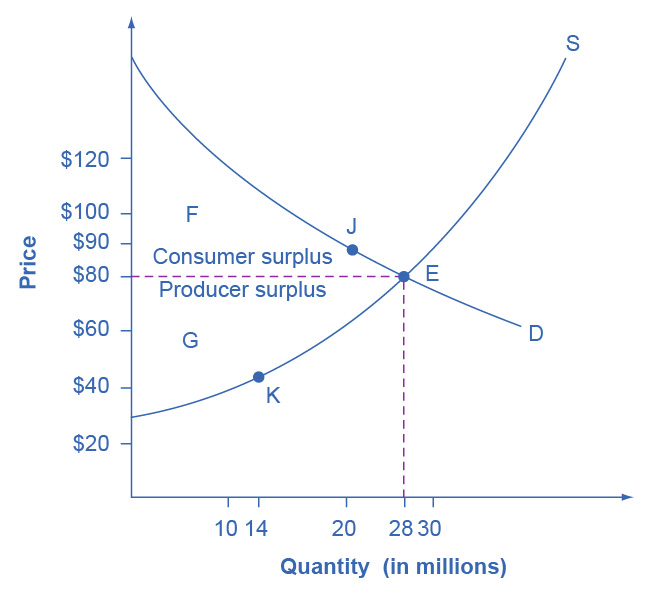
\includegraphics[width=3.25in,height=2.995in]{media/3-5-demand-supply-and-efficiency_rId26.jpeg}

Figure 3.23 Consumer and Producer Surplus The somewhat triangular area
labeled by F shows the area of consumer surplus, which shows that the
equilibrium price in the market was less than what many of the consumers
were willing to pay. Point J on the demand curve shows that, even at the
price of \$90, consumers would have been willing to purchase a quantity
of 20 million. The somewhat triangular area labeled by G shows the area
of producer surplus, which shows that the equilibrium price received in
the market was more than what many of the producers were willing to
accept for their products. For example, point K on the supply curve
shows that at a price of \$45, firms would have been willing to supply a
quantity of 14 million.

The supply curve shows the quantity that firms are willing to supply at
each price. For example, point K in
\protect\hyperlink{CNX_Econ_C03_015}{Figure 3.23} illustrates that, at
\$45, firms would still have been willing to supply a quantity of 14
million. Those producers who would have been willing to supply the
tablets at \$45, but who were instead able to charge the equilibrium
price of \$80, clearly received an extra benefit beyond what they
required to supply the product. The extra benefit producers receive from
selling a good or service, measured by the price the producer actually
received minus the price the producer would have been willing to accept
is called producer surplus. In
\protect\hyperlink{CNX_Econ_C03_015}{Figure 3.23}, producer surplus is
the area labeled G---that is, the area between the market price and the
segment of the supply curve below the equilibrium.

The sum of consumer surplus and producer surplus is social surplus, also
referred to as economic surplus or total surplus. In
\protect\hyperlink{CNX_Econ_C03_015}{Figure 3.23} we show social surplus
as the area F + G. Social surplus is larger at equilibrium quantity and
price than it would be at any other quantity. This demonstrates the
economic efficiency of the market equilibrium. In addition, at the
efficient level of output, it is impossible to produce greater consumer
surplus without reducing producer surplus, and it is impossible to
produce greater producer surplus without reducing consumer surplus.

\hypertarget{inefficiency-of-price-floors-and-price-ceilings}{%
\subsection{Inefficiency of Price Floors and Price
Ceilings}\label{inefficiency-of-price-floors-and-price-ceilings}}

The imposition of a price floor or a price ceiling will prevent a market
from adjusting to its equilibrium price and quantity, and thus will
create an inefficient outcome. However, there is an additional twist
here. Along with creating inefficiency, price floors and ceilings will
also transfer some consumer surplus to producers, or some producer
surplus to consumers.

Imagine that several firms develop a promising but expensive new drug
for treating back pain. If this therapy is left to the market, the
equilibrium price will be \$600 per month and 20,000 people will use the
drug, as shown in \protect\hyperlink{CNX_Econ_C03_028}{Figure 3.24} (a).
The original level of consumer surplus is T + U and producer surplus is
V + W + X. However, the government decides to impose a price ceiling of
\$400 to make the drug more affordable. At this price ceiling, firms in
the market now produce only 15,000.

As a result, two changes occur. First, an inefficient outcome occurs and
the total surplus of society is reduced. The loss in social surplus that
occurs when the economy produces at an inefficient quantity is called
deadweight loss. In a very real sense, it is like money thrown away that
benefits no one. In \protect\hyperlink{CNX_Econ_C03_028}{Figure 3.24}
(a), the deadweight loss is the area U + W. When deadweight loss exists,
it is possible for both consumer and producer surplus to be higher, in
this case because the price control is blocking some suppliers and
demanders from transactions they would both be willing to make.

A second change from the price ceiling is that some of the producer
surplus is transferred to consumers. After the price ceiling is imposed,
the new consumer surplus is T + V, while the new producer surplus is X.
In other words, the price ceiling transfers the area of surplus (V) from
producers to consumers. Note that the gain to consumers is less than the
loss to producers, which is just another way of seeing the deadweight
loss.

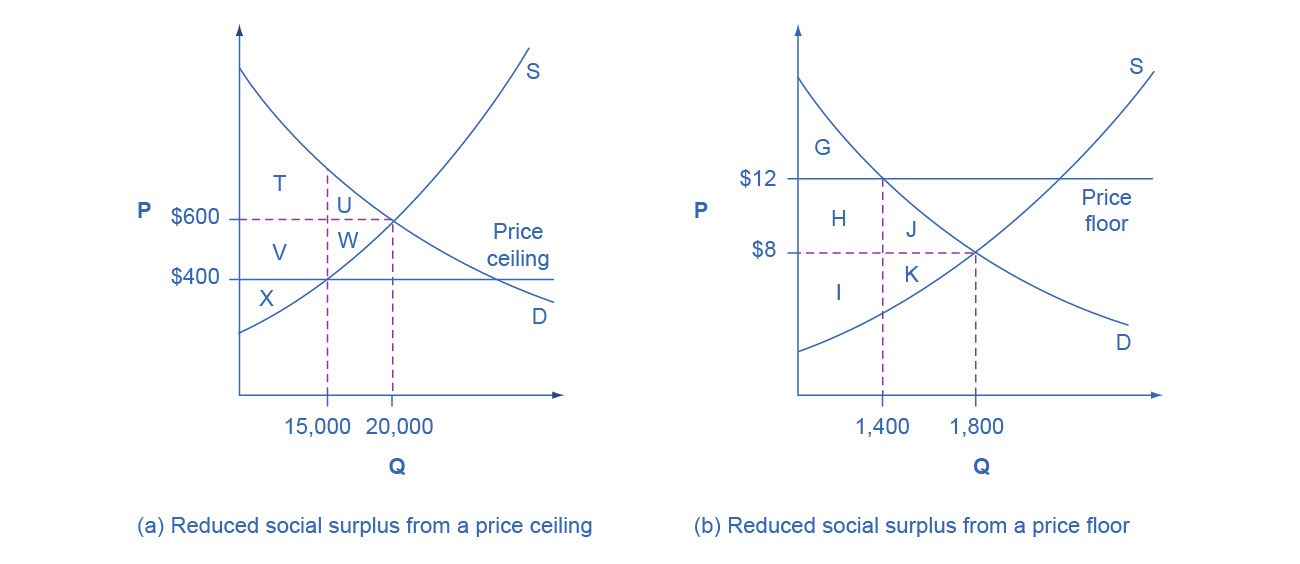
\includegraphics[width=6.5in,height=2.82in]{media/3-5-demand-supply-and-efficiency_rId38.jpeg}

Figure 3.24 Efficiency and Price Floors and Ceilings (a) The original
equilibrium price is \$600 with a quantity of 20,000. Consumer surplus
is T + U, and producer surplus is V + W + X. A price ceiling is imposed
at \$400, so firms in the market now produce only a quantity of 15,000.
As a result, the new consumer surplus is T + V, while the new producer
surplus is X. (b) The original equilibrium is \$8 at a quantity of
1,800. Consumer surplus is G + H + J, and producer surplus is I + K. A
price floor is imposed at \$12, which means that quantity demanded falls
to 1,400. As a result, the new consumer surplus is G, and the new
producer surplus is H + I.

\protect\hyperlink{CNX_Econ_C03_028}{Figure 3.24} (b) shows a price
floor example using a string of struggling movie theaters, all in the
same city. The current equilibrium is \$8 per movie ticket, with 1,800
people attending movies. The original consumer surplus is G + H + J, and
producer surplus is I + K. The city government is worried that movie
theaters will go out of business, reducing the entertainment options
available to citizens, so it decides to impose a price floor of \$12 per
ticket. As a result, the quantity demanded of movie tickets falls to
1,400. The new consumer surplus is G, and the new producer surplus is H
+ I. In effect, the price floor causes the area H to be transferred from
consumer to producer surplus, but also causes a deadweight loss of J +
K.

This analysis shows that a price ceiling, like a law establishing rent
controls, will transfer some producer surplus to consumers---which helps
to explain why consumers often favor them. Conversely, a price floor
like a guarantee that farmers will receive a certain price for their
crops will transfer some consumer surplus to producers, which explains
why producers often favor them. However, both price floors and price
ceilings block some transactions that buyers and sellers would have been
willing to make, and creates deadweight loss. Removing such barriers, so
that prices and quantities can adjust to their equilibrium level, will
increase the economy's social surplus.

\hypertarget{demand-and-supply-as-a-social-adjustment-mechanism}{%
\subsection{Demand and Supply as a Social Adjustment
Mechanism}\label{demand-and-supply-as-a-social-adjustment-mechanism}}

The demand and supply model emphasizes that prices are not set only by
demand or only by supply, but by the interaction between the two. In
1890, the famous economist Alfred Marshall wrote that asking whether
supply or demand determined a price was like arguing ``whether it is the
upper or the under blade of a pair of scissors that cuts a piece of
paper.'' The answer is that both blades of the demand and supply
scissors are always involved.

The adjustments of equilibrium price and quantity in a market-oriented
economy often occur without much government direction or oversight. If
the coffee crop in Brazil suffers a terrible frost, then the supply
curve of coffee shifts to the left and the price of coffee rises. Some
people continue to drink coffee and pay the higher price. Others switch
to tea or soft drinks. No government commission is needed to figure out
how to adjust coffee prices, which companies will be allowed to process
the remaining supply, which supermarkets in which cities will get how
much coffee to sell, or which consumers will ultimately be allowed to
drink the brew. Such adjustments in response to price changes happen all
the time in a market economy, often so smoothly and rapidly that we
barely notice them.

Think for a moment of all the seasonal foods that are available and
inexpensive at certain times of the year, like fresh corn in midsummer,
but more expensive at other times of the year. People alter their diets
and restaurants alter their menus in response to these fluctuations in
prices without fuss or fanfare. For both the U.S. economy and the world
economy as a whole, markets---that is, demand and supply---are the
primary social mechanism for answering the basic questions about what is
produced, how it is produced, and for whom it is produced.

\hypertarget{bring-it-home}{%
\subsection{Bring It Home}\label{bring-it-home}}

\hypertarget{why-can-we-not-get-enough-of-organic-food}{%
\subsubsection{Why Can We Not Get Enough of Organic
Food?}\label{why-can-we-not-get-enough-of-organic-food}}

Organic food is grown without synthetic pesticides, chemical fertilizers
or genetically modified seeds. In recent decades, the demand for organic
products has increased dramatically. The Organic Trade Association
reported sales increased from \$1 billion in 1990 to nearly \$62 billion
in 2020, more than 90\% of which were sales of food products.

Why, then, are organic foods more expensive than their conventional
counterparts? The answer is a clear application of the theories of
supply and demand. As people have learned more about the harmful effects
of chemical fertilizers, growth hormones, pesticides and the like from
large-scale factory farming, our tastes and preferences for safer,
organic foods have increased. This change in tastes has been reinforced
by increases in income, which allow people to purchase pricier products,
and has made organic foods more mainstream. This shift, in addition to
population growth, has led to an increased demand for organic foods.
Graphically, the demand curve has shifted right, and we have moved up
the supply curve as producers have responded to the higher prices by
supplying a greater quantity.

In addition to the movement along the supply curve, we have also had an
increase in the number of farmers converting to organic farming over
time. This is represented by a shift to the right of the supply curve.
Since both demand and supply have shifted to the right, the resulting
equilibrium quantity of organic foods is definitely higher, but the
price will only fall when the increase in supply is larger than the
increase in demand. We may need more time before we see lower prices in
organic foods. Since the production costs of these foods may remain
higher than conventional farming, because organic fertilizers and pest
management techniques are more expensive, they may never fully catch up
with the lower prices of non-organic foods.

As a final, specific example: The Environmental Working Group's ``Dirty
Dozen'' list of fruits and vegetables, which test high for pesticide
residue even after washing, was released in April 2013. The inclusion of
strawberries on the list led to an increase in demand for organic
strawberries, resulting in both a higher equilibrium price and quantity
of sales.

\part{4-Labor and Financial Markets}

\hypertarget{chapter-objectives}{%
\chapter{Chapter Objectives}\label{chapter-objectives}}


\includegraphics[width=6.5in,height=3.93333in]{media/4-introduction-to-labor-and-financial-markets_rId20.jpeg}

Figure 4.1 People often think of demand and supply in relation to goods,
but labor markets, such as the nursing profession, can also apply to
this analysis. (Credit: modification of "Hospital do Subúrbio" by Jaques
Wagner Governador/Flickr Creative Commons, CC BY 2.0)

In this chapter, you will learn about:

\begin{itemize}
\tightlist
\item
  Demand and Supply at Work in Labor Markets
\item
  Demand and Supply in Financial Markets
\item
  The Market System as an Efficient Mechanism for Information
\end{itemize}

\hypertarget{introduction-to-labor-and-financial-markets}{%
\section{Introduction to Labor and Financial
Markets}\label{introduction-to-labor-and-financial-markets}}

\hypertarget{bring-it-home}{%
\subsection{Bring It Home}\label{bring-it-home}}

\hypertarget{baby-boomers-come-of-age}{%
\subsubsection{Baby Boomers Come of
Age}\label{baby-boomers-come-of-age}}

According to the 2020 Census, 22\% of the U.S. population was 60 years
old or older, which means that more than 74 million people have reached
an age when they will need increased medical care.

The baby boomer population, the group born between 1946 and 1964, is
comprised of more than 71 million people who have already reached
retirement age or will soon reach retirement. As this population grows
older, they will be faced with common healthcare issues such as heart
conditions, arthritis, and Alzheimer's that may require hospitalization,
long-term, or at-home nursing care. Aging baby boomers and advances in
life-saving and life-extending technologies will increase the demand for
healthcare and nursing. Additionally, the Affordable Care Act, which
expands access to healthcare for millions of Americans, has further
increased the demand.

These data tell us, as economists, that the market for healthcare
professionals, and nurses in particular, will face several challenges.
Our study of supply and demand will help us to analyze what might happen
in the labor market for nursing and other healthcare professionals, as
we will discuss in the second half of this case at the end of the
chapter.

The theories of supply and demand do not apply just to markets for
goods. They apply to any market, even markets for things we may not
think of as goods and services like labor and financial services. Labor
markets are markets for employees or jobs. Financial services markets
are markets for saving or borrowing.

When we think about demand and supply curves in goods and services
markets, it is easy to picture the demanders and suppliers: businesses
produce the products and households buy them. Who are the demanders and
suppliers in labor and financial service markets? In labor markets job
seekers (individuals) are the suppliers of labor, while firms and other
employers who hire labor are the demanders for labor. In financial
markets, any individual or firm who saves contributes to the supply of
money, and any entity that borrows (person, firm, or government)
contributes to the demand for money.

As a college student, you most likely participate in both labor and
financial markets. Employment is a fact of life for most college
students: According to the National Center for Educational Statistics,
in 2018 43\% of full-time college students and 81\% of part-time college
students were employed. Most college students are also heavily involved
in financial markets, primarily as borrowers. As of the 2018--19 school
year, 43\% of full-time undergraduate students were receiving loan aid
to help finance their education, and those loans averaged \$7,300 per
year. Many students also borrow for other expenses, like purchasing a
car. As this chapter will illustrate, we can analyze labor markets and
financial markets with the same tools we use to analyze demand and
supply in the goods markets.

\hypertarget{demand-and-supply-at-work-in-labor-markets}{%
\chapter{4.1 Demand and Supply at Work in Labor
Markets}\label{demand-and-supply-at-work-in-labor-markets}}

\hypertarget{learning-objectives-12}{%
\subsection{Learning Objectives}\label{learning-objectives-12}}

By the end of this section, you will be able to:

\begin{itemize}
\tightlist
\item
  Predict shifts in the demand and supply curves of the labor market
\item
  Explain the impact of new technology on the demand and supply curves
  of the labor market
\item
  Explain price floors in the labor market such as minimum wage or a
  living wage
\end{itemize}

Markets for labor have demand and supply curves, just like markets for
goods. The law of demand applies in labor markets this way: A higher
salary or wage---that is, a higher price in the labor market---leads to
a decrease in the quantity of labor demanded by employers, while a lower
salary or wage leads to an increase in the quantity of labor demanded.
The law of supply functions in labor markets, too: A higher price for
labor leads to a higher quantity of labor supplied; a lower price leads
to a lower quantity supplied.

\hypertarget{equilibrium-in-the-labor-market}{%
\subsection{Equilibrium in the Labor
Market}\label{equilibrium-in-the-labor-market}}

In 2020, nearly 41,000 registered nurses worked in the Minneapolis-St.
Paul-Bloomington, Minnesota-Wisconsin metropolitan area, according to
the BLS. They worked for a variety of employers: hospitals, doctors'
offices, schools, health clinics, and nursing homes.
\protect\hyperlink{CNX_Econ_C04_001}{Figure 4.2} illustrates how demand
and supply determine equilibrium in this labor market. The demand and
supply schedules in \protect\hyperlink{Table_04_01}{Table 4.1} list the
quantity supplied and quantity demanded of nurses at different salaries.

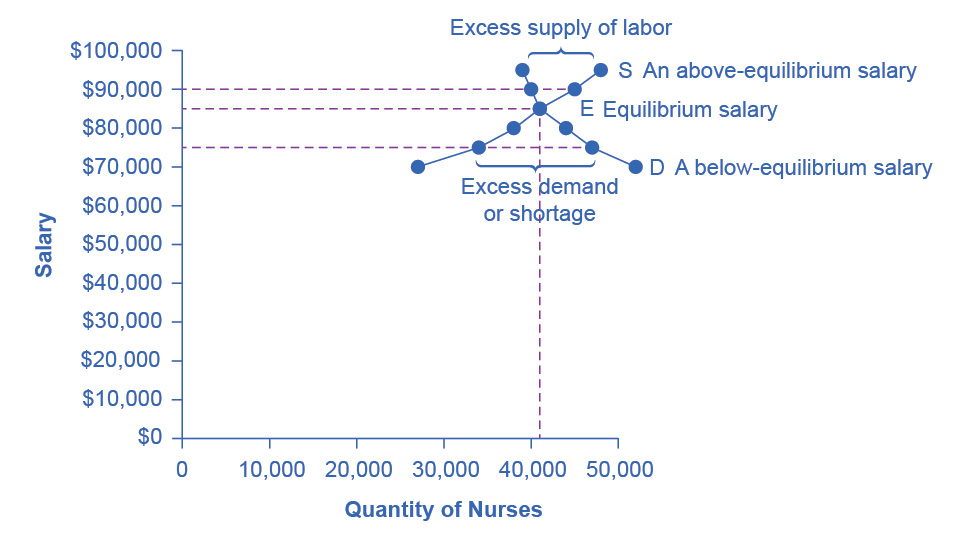
\includegraphics[width=4.88in,height=2.68in]{media/4-1-demand-and-supply-at-work-in-labor-markets_rId24.jpeg}

Figure 4.2 Labor Market Example: Demand and Supply for Nurses in
Minneapolis-St.~Paul-Bloomington The demand curve (D) of those employers
who want to hire nurses intersects with the supply curve (S) of those
who are qualified and willing to work as nurses at the equilibrium point
(E). The equilibrium salary is \$85,000 and the equilibrium quantity is
41,000 nurses. At an above-equilibrium salary of \$90,000, quantity
supplied increases to 45,000, but the quantity of nurses demanded at the
higher pay declines to 40,000. At this above-equilibrium salary, an
excess supply or surplus of nurses would exist. At a below-equilibrium
salary of \$75,000, quantity supplied declines to 34,000, while the
quantity demanded at the lower wage increases to 47,000 nurses. At this
below-equilibrium salary, excess demand or a shortage exists.

Table 4.1 Demand and Supply of Nurses in Minneapolis-St.
Paul-Bloomington

The horizontal axis shows the quantity of nurses hired. In this example
we measure labor by number of workers, but another common way to measure
the quantity of labor is by the number of hours worked. The vertical
axis shows the price for nurses' labor---that is, how much they are
paid. In the real world, this ``price'' would be total labor
compensation: salary plus benefits. It is not obvious, but benefits are
a significant part (as high as 30 percent) of labor compensation. In
this example we measure the price of labor by salary on an annual basis,
although in other cases we could measure the price of labor by monthly
or weekly pay, or even the wage paid per hour. As the salary for nurses
rises, the quantity demanded will fall. Some hospitals and nursing homes
may reduce the number of nurses they hire, or they may lay off some of
their existing nurses, rather than pay them higher salaries. Employers
who face higher nurses' salaries may also try to replace some nursing
functions by investing in physical equipment, like computer monitoring
and diagnostic systems to monitor patients, or by using lower-paid
health care aides to reduce the number of nurses they need.

As the salary for nurses rises, the quantity supplied will rise. If
nurses' salaries in Minneapolis-St.~Paul-Bloomington are higher than in
other cities, more nurses will move to Minneapolis-St.~Paul-Bloomington
to find jobs, more people will be willing to train as nurses, and those
currently trained as nurses will be more likely to pursue nursing as a
full-time job. In other words, there will be more nurses looking for
jobs in the area.

At equilibrium, the quantity supplied and the quantity demanded are
equal. Thus, every employer who wants to hire a nurse at this
equilibrium wage can find a willing worker, and every nurse who wants to
work at this equilibrium salary can find a job. In
\protect\hyperlink{CNX_Econ_C04_001}{Figure 4.2}, the supply curve (S)
and demand curve (D) intersect at the equilibrium point (E). The
equilibrium quantity of nurses in the Minneapolis-St.~Paul-Bloomington
area is 41,000, and the equilibrium salary is \$86,000 per year. This
example simplifies the nursing market by focusing on the ``average''
nurse. In reality, of course, the market for nurses actually comprises
many smaller markets, like markets for nurses with varying degrees of
experience and credentials. Many markets contain closely related
products that differ in quality. For instance, even a simple product
like gasoline comes in regular, premium, and super-premium, each with a
different price. Even in such cases, discussing the average price of
gasoline, like the average salary for nurses, can still be useful
because it reflects what is happening in most of the submarkets.

When the price of labor is not at the equilibrium, economic incentives
tend to move salaries toward the equilibrium. For example, if salaries
for nurses in Minneapolis-St.~Paul-Bloomington were above the
equilibrium at \$90,000 per year, then 43,000 people want to work as
nurses, but employers want to hire only 39,000 nurses. At that
above-equilibrium salary, excess supply or a surplus results. In a
situation of excess supply in the labor market, with many applicants for
every job opening, employers will have an incentive to offer lower wages
than they otherwise would have. Nurses' salary will move down toward
equilibrium.

In contrast, if the salary is below the equilibrium at, say, \$60,000
per year, then a situation of excess demand or a shortage arises. In
this case, employers encouraged by the relatively lower wage want to
hire 40,000 nurses, but only 27,000 individuals want to work as nurses
at that salary in Minneapolis-St.~Paul-Bloomington. In response to the
shortage, some employers will offer higher pay to attract the nurses.
Other employers will have to match the higher pay to keep their own
employees. The higher salaries will encourage more nurses to train or
work in Minneapolis-St.~Paul-Bloomington. Again, price and quantity in
the labor market will move toward equilibrium.

\hypertarget{shifts-in-labor-demand}{%
\subsection{Shifts in Labor Demand}\label{shifts-in-labor-demand}}

The demand curve for labor shows the quantity of labor employers wish to
hire at any given salary or wage rate, under the \emph{ceteris paribus}
assumption. A change in the wage or salary will result in a change in
the quantity demanded of labor. If the wage rate increases, employers
will want to hire fewer employees. The quantity of labor demanded will
decrease, and there will be a movement upward along the demand curve. If
the wages and salaries decrease, employers are more likely to hire a
greater number of workers. The quantity of labor demanded will increase,
resulting in a downward movement along the demand curve.

Shifts in the demand curve for labor occur for many reasons. One key
reason is that the demand for labor is based on the demand for the good
or service that is produced. For example, the more new automobiles
consumers demand, the greater the number of workers automakers will need
to hire. Therefore the demand for labor is called a ``derived demand.''
Here are some examples of derived demand for labor:

\begin{itemize}
\tightlist
\item
  The demand for chefs is dependent on the demand for restaurant meals.
\item
  The demand for pharmacists is dependent on the demand for prescription
  drugs.
\item
  The demand for attorneys is dependent on the demand for legal
  services.
\end{itemize}

As the demand for the goods and services increases, the demand for labor
will increase, or shift to the right, to meet employers' production
requirements. As the demand for the goods and services decreases, the
demand for labor will decrease, or shift to the left.
\protect\hyperlink{Table_04_02}{Table 4.2} shows that in addition to the
derived demand for labor, demand can also increase or decrease (shift)
in response to several factors.

Table 4.2 Factors That Can Shift Demand

\hypertarget{link-it-up}{%
\subsection{Link It Up}\label{link-it-up}}

Click \href{http://openstax.org/l/Futurework}{here} to read more about
``Trends and Challenges for Work in the 21\textsuperscript{st}
Century.''

\hypertarget{shifts-in-labor-supply}{%
\subsection{Shifts in Labor Supply}\label{shifts-in-labor-supply}}

The supply of labor is upward-sloping and adheres to the law of supply:
The higher the price, the greater the quantity supplied and the lower
the price, the less quantity supplied. The supply curve models the
tradeoff between supplying labor into the market or using time in
leisure activities at every given price level. The higher the wage, the
more labor is willing to work and forego leisure activities.
\protect\hyperlink{Table_04_03}{Table 4.3} lists some of the factors
that will cause the supply to increase or decrease.

Table 4.3 Factors that Can Shift Supply

A change in salary will lead to a movement along labor demand or labor
supply curves, but it will not shift those curves. However, other events
like those we have outlined here will cause either the demand or the
supply of labor to shift, and thus will move the labor market to a new
equilibrium salary and quantity.

\hypertarget{technology-and-wage-inequality-the-four-step-process}{%
\subsection{Technology and Wage Inequality: The Four-Step
Process}\label{technology-and-wage-inequality-the-four-step-process}}

Economic events can change the equilibrium salary (or wage) and quantity
of labor. Consider how the wave of new information technologies, like
computer and telecommunications networks, has affected low-skill and
high-skill workers in the U.S. economy. From the perspective of
employers who demand labor, these new technologies are often a
substitute for low-skill laborers like file clerks who used to keep file
cabinets full of paper records of transactions. However, the same new
technologies are a complement to high-skill workers like managers, who
benefit from the technological advances by having the ability to monitor
more information, communicate more easily, and juggle a wider array of
responsibilities. How will the new technologies affect the wages of
high-skill and low-skill workers? For this question, the four-step
process of analyzing how shifts in supply or demand affect a market
(introduced in
\href{http://openstax.org/books/principles-microeconomics-3e/pages/3-introduction-to-demand-and-supply}{Demand
and Supply}) works in this way:

Step 1. What did the markets for low-skill labor and high-skill labor
look like before the arrival of the new technologies? In
\protect\hyperlink{CNX_Econ_C04_009}{Figure 4.3} (a) and
\protect\hyperlink{CNX_Econ_C04_009}{Figure 4.3} (b), S\textsubscript{0}
is the original supply curve for labor and D\textsubscript{0} is the
original demand curve for labor in each market. In each graph, the
original point of equilibrium, E\textsubscript{0}, occurs at the price
W\textsubscript{0} and the quantity Q\textsubscript{0}.

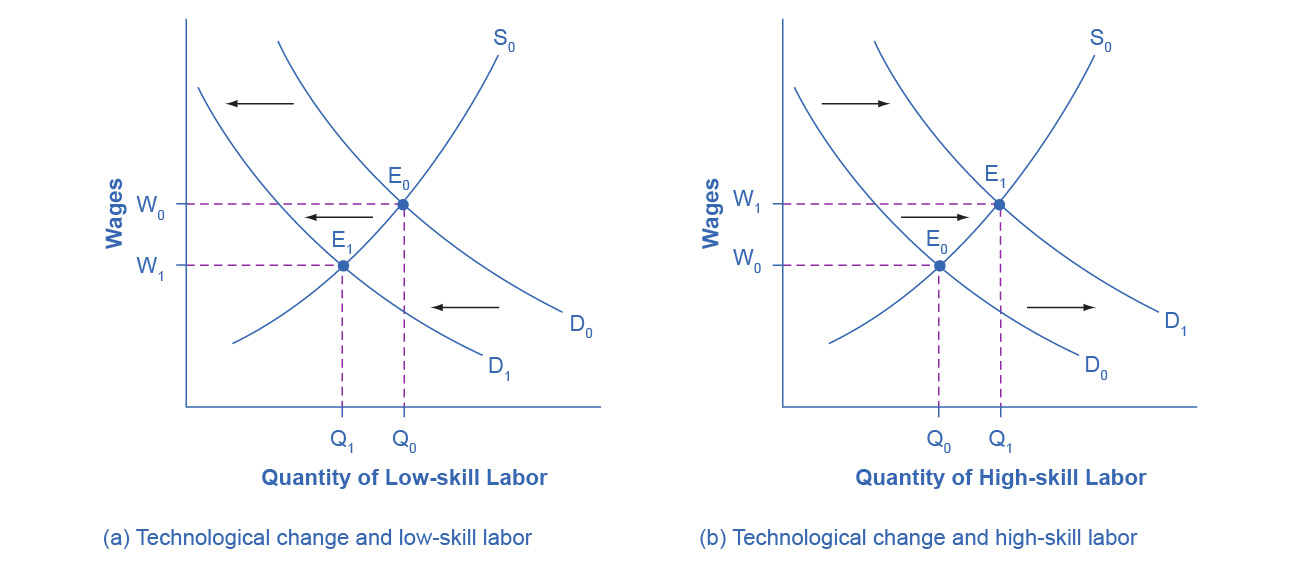
\includegraphics[width=6.5in,height=2.855in]{media/4-1-demand-and-supply-at-work-in-labor-markets_rId39.jpeg}

Figure 4.3 Technology and Wages: Applying Demand and Supply (a) The
demand for low-skill labor shifts to the left when technology can do the
job previously done by these workers. (b) New technologies can also
increase the demand for high-skill labor in fields such as information
technology and network administration.

Step 2. Does the new technology affect the supply of labor from
households or the demand for labor from firms? The technology change
described here affects demand for labor by firms that hire workers.

Step 3. Will the new technology increase or decrease demand? Based on
the description earlier, as the substitute for low-skill labor becomes
available, demand for low-skill labor will shift to the left, from
D\textsubscript{0} to D\textsubscript{1}. As the technology complement
for high-skill labor becomes cheaper, demand for high-skill labor will
shift to the right, from D\textsubscript{0} to D\textsubscript{1}.

Step 4. The new equilibrium for low-skill labor, shown as point
E\textsubscript{1} with price W\textsubscript{1} and quantity
Q\textsubscript{1}, has a lower wage and quantity hired than the
original equilibrium, E\textsubscript{0}. The new equilibrium for
high-skill labor, shown as point E\textsubscript{1} with price
W\textsubscript{1} and quantity Q\textsubscript{1}, has a higher wage
and quantity hired than the original equilibrium (E\textsubscript{0}).

Thus, the demand and supply model predicts that the new computer and
communications technologies will raise the pay of high-skill workers but
reduce the pay of low-skill workers. From the 1970s to the mid-2000s,
the wage gap widened between high-skill and low-skill labor. According
to the National Center for Education Statistics, in 1980, for example, a
college graduate earned about 30\% more than a high school graduate with
comparable job experience, but by 2019, a college graduate earned about
59\% more than an otherwise comparable high school graduate. Many
economists believe that the trend toward greater wage inequality across
the U.S. economy is due to improvements in technology.

\hypertarget{link-it-up-1}{%
\subsection{Link It Up}\label{link-it-up-1}}

Visit this \href{http://openstax.org/l/oldtechjobs}{website} to read
about ten tech skills that have lost relevance in today's workforce.

\hypertarget{price-floors-in-the-labor-market-living-wages-and-minimum-wages}{%
\subsection{Price Floors in the Labor Market: Living Wages and Minimum
Wages}\label{price-floors-in-the-labor-market-living-wages-and-minimum-wages}}

In contrast to goods and services markets, price ceilings are rare in
labor markets, because rules that prevent people from earning income are
not politically popular. There is one exception: boards of trustees or
stockholders, as an example, propose limits on the high incomes of top
business executives.

The labor market, however, presents some prominent examples of price
floors, which are an attempt to increase the wages of low-paid workers.
The U.S. government sets a minimum wage, a price floor that makes it
illegal for an employer to pay employees less than a certain hourly
rate. In mid-2009, the U.S. minimum wage was raised to \$7.25 per hour.
Local political movements in a number of U.S. cities have pushed for a
higher minimum wage, which they call a living wage. Promoters of living
wage laws maintain that the minimum wage is too low to ensure a
reasonable standard of living. They base this conclusion on the
calculation that, if you work 40 hours a week at a minimum wage of
\$7.25 per hour for 50 weeks a year, your annual income is \$14,500,
which is less than the official U.S. government definition of what it
means for a family to be in poverty. (A family with two adults earning
minimum wage and two young children will find it more cost efficient for
one parent to provide childcare while the other works for income. Thus
the family income would be \$14,500, which is significantly lower than
the federal poverty line for a family of four, which was \$26,500 in
2021.)

Supporters of the living wage argue that full-time workers should be
assured a high enough wage so that they can afford the essentials of
life: food, clothing, shelter, and healthcare. Since Baltimore passed
the first living wage law in 1994, several dozen cities enacted similar
laws in the late 1990s and the 2000s. The living wage ordinances do not
apply to all employers, but they have specified that all employees of
the city or employees of firms that the city hires be paid at least a
certain wage that is usually a few dollars per hour above the U.S.
minimum wage.

\protect\hyperlink{CNX_Econ_C04_004}{Figure 4.4} illustrates the
situation of a city considering a living wage law. For simplicity, we
assume that there is no federal minimum wage. The wage appears on the
vertical axis, because the wage is the price in the labor market. Before
the passage of the living wage law, the equilibrium wage is \$10 per
hour and the city hires 1,200 workers at this wage. However, a group of
concerned citizens persuades the city council to enact a living wage law
requiring employers to pay no less than \$12 per hour. In response to
the higher wage, 1,600 workers look for jobs with the city. At this
higher wage, the city, as an employer, is willing to hire only 700
workers. At the price floor, the quantity supplied exceeds the quantity
demanded, and a surplus of labor exists in this market. For workers who
continue to have a job at a higher salary, life has improved. For those
who were willing to work at the old wage rate but lost their jobs with
the wage increase, life has not improved.
\protect\hyperlink{Table_04_04}{Table 4.4} shows the differences in
supply and demand at different wages.

\includegraphics[width=3.25in,height=2.49in]{media/4-1-demand-and-supply-at-work-in-labor-markets_rId48.jpeg}

Figure 4.4 A Living Wage: Example of a Price Floor The original
equilibrium in this labor market is a wage of \$10/hour and a quantity
of 1,200 workers, shown at point E. Imposing a wage floor at \$12/hour
leads to an excess supply of labor. At that wage, the quantity of labor
supplied is 1,600 and the quantity of labor demanded is only 700.

Table 4.4 Living Wage: Example of a Price Floor

\hypertarget{the-minimum-wage-as-an-example-of-a-price-floor}{%
\subsection{The Minimum Wage as an Example of a Price
Floor}\label{the-minimum-wage-as-an-example-of-a-price-floor}}

The U.S. minimum wage is a price floor that is set either very close to
the equilibrium wage or even slightly below it. About 1.5\% of hourly
workers in the U.S. are paid the minimum wage. In other words, the vast
majority of the U.S. labor force has its wages determined in the labor
market, not as a result of the government price floor. However, for
workers with low skills and little experience, like those without a high
school diploma or teenagers, the minimum wage is quite important. In
many cities, the federal minimum wage is apparently below the market
price for unskilled labor, because employers offer more than the minimum
wage to checkout clerks and other low-skill workers without any
government prodding.

Economists have attempted to estimate how much the minimum wage reduces
the quantity demanded of low-skill labor. A typical result of such
studies is that a 10\% increase in the minimum wage would decrease the
hiring of unskilled workers by 1 to 2\%, which seems a relatively small
reduction. In fact, some studies have even found no effect of a higher
minimum wage on employment at certain times and places---although these
studies are controversial. Well-known economists Walter Williams and
Thomas Sowell, who both focus on the intersections of race and
economics, argue that minimum wages increase discrimination and limit
economic mobility. Williams, for example, indicates that higher minimum
wages would increase employment barriers for lower-skilled workers,
reducing the opportunity for them to learn on the job and gain
experience that would give them more choice in employment.

Let's suppose that the minimum wage lies just slightly \emph{below} the
equilibrium wage level. Wages could fluctuate according to market forces
above this price floor, but they would not be allowed to move beneath
the floor. In this situation, the price floor minimum wage is
\emph{nonbinding} ---that is, the price floor is not determining the
market outcome. Even if the minimum wage moves just a little higher, it
will still have no effect on the quantity of employment in the economy,
as long as it remains below the equilibrium wage. Even if the government
increases the minimum wage by enough so that it rises slightly above the
equilibrium wage and becomes binding, there will be only a small excess
supply gap between the quantity demanded and quantity supplied.

These insights help to explain why U.S. minimum wage laws have
historically had only a small impact on employment. Since the minimum
wage has typically been set close to the equilibrium wage for low-skill
labor and sometimes even below it, it has not had a large effect in
creating an excess supply of labor. However, if the minimum wage
increased dramatically---say, if it doubled to match the living wages
that some U.S. cities have considered---then its impact on reducing the
quantity demanded of employment would be far greater. The following
Clear It Up feature describes in greater detail some of the arguments
for and against changes to the minimum wage.

\hypertarget{clear-it-up}{%
\subsection{Clear It Up}\label{clear-it-up}}

\hypertarget{whats-the-harm-in-raising-the-minimum-wage}{%
\subsubsection{What's the harm in raising the minimum
wage?}\label{whats-the-harm-in-raising-the-minimum-wage}}

Because of the law of demand, a higher required wage will reduce the
amount of low-skill employment either in terms of employees or in terms
of work hours. Although there is controversy over the numbers, let's say
for the sake of the argument that a 10\% rise in the minimum wage will
reduce the employment of low-skill workers by 2\%. Does this outcome
mean that raising the minimum wage by 10\% is bad public policy? Not
necessarily.

If 98\% of those receiving the minimum wage have a pay increase of 10\%,
but 2\% of those receiving the minimum wage lose their jobs, are the
gains for society as a whole greater than the losses? The answer is not
clear, because job losses, even for a small group, may cause more pain
than modest income gains for others. For one thing, we need to consider
which minimum wage workers are losing their jobs. If the 2\% of minimum
wage workers who lose their jobs are struggling to support families,
that is one thing. If those who lose their job are high school students
picking up spending money over summer vacation, that is something else.

Another complexity is that many minimum wage workers do not work
full-time for an entire year. Imagine a minimum wage worker who holds
different part-time jobs for a few months at a time, with bouts of
unemployment in between. The worker in this situation receives the 10\%
raise in the minimum wage when working, but also ends up working 2\%
fewer hours during the year because the higher minimum wage reduces how
much employers want people to work. Overall, this worker's income would
rise because the 10\% pay raise would more than offset the 2\% fewer
hours worked.

Of course, these arguments do not prove that raising the minimum wage is
necessarily a good idea either. There may well be other, better public
policy options for helping low-wage workers. (The
\href{http://openstax.org/books/principles-microeconomics-3e/pages/15-introduction-to-poverty-and-economic-inequality}{Poverty
and Economic Inequality} chapter discusses some possibilities.) The
lesson from this maze of minimum wage arguments is that complex social
problems rarely have simple answers. Even those who agree on how a
proposed economic policy affects quantity demanded and quantity supplied
may still disagree on whether the policy is a good idea.

\hypertarget{demand-and-supply-in-financial-markets}{%
\chapter{4.2 Demand and Supply in Financial
Markets}\label{demand-and-supply-in-financial-markets}}

\hypertarget{learning-objectives-13}{%
\subsection{Learning Objectives}\label{learning-objectives-13}}

By the end of this section, you will be able to:

\begin{itemize}
\tightlist
\item
  Identify the demanders and suppliers in a financial market
\item
  Explain how interest rates can affect supply and demand
\item
  Analyze the economic effects of U.S. debt in terms of domestic
  financial markets
\item
  Explain the role of price ceilings and usury laws in the U.S.
\end{itemize}

United States\textquotesingle{} households, institutions, and domestic
businesses saved almost \$1.3 trillion in 2015. Where did that savings
go and how was it used? Some of the savings ended up in banks, which in
turn loaned the money to individuals or businesses that wanted to borrow
money. Some was invested in private companies or loaned to government
agencies that wanted to borrow money to raise funds for purposes like
building roads or mass transit. Some firms reinvested their savings in
their own businesses.

In this section, we will determine how the demand and supply model links
those who wish to supply financial capital (i.e., savings) with those
who demand financial capital (i.e., borrowing). Those who save money (or
make financial investments, which is the same thing), whether
individuals or businesses, are on the supply side of the financial
market. Those who borrow money are on the demand side of the financial
market. For a more detailed treatment of the different kinds of
financial investments like bank accounts, stocks and bonds, see the
\href{http://openstax.org/books/principles-microeconomics-3e/pages/17-introduction-to-financial-markets}{Financial
Markets} chapter.

\hypertarget{who-demands-and-who-supplies-in-financial-markets}{%
\subsection{Who Demands and Who Supplies in Financial
Markets?}\label{who-demands-and-who-supplies-in-financial-markets}}

In any market, the price is what suppliers receive and what demanders
pay. In financial markets, those who supply financial capital through
saving expect to receive a rate of return, while those who demand
financial capital by receiving funds expect to pay a rate of return.
This rate of return can come in a variety of forms, depending on the
type of investment.

The simplest example of a rate of return is the interest rate. For
example, when you supply money into a savings account at a bank, you
receive interest on your deposit. The interest the bank pays you as a
percent of your deposits is the interest rate. Similarly, if you demand
a loan to buy a car or a computer, you will need to pay interest on the
money you borrow.

Let's consider the market for borrowing money with credit cards. In
2021, almost 200 million Americans were cardholders. Credit cards allow
you to borrow money from the card\textquotesingle s issuer, and pay back
the borrowed amount plus interest, although most allow you a period of
time in which you can repay the loan without paying interest. A typical
credit card interest rate ranges from 12\% to 18\% per year. In May
2021, Americans had about \$807 billion outstanding in credit card
debts. As of 2021, just over 45\% of American families carried some
credit card debt. Let's say that, on average, the annual interest rate
for credit card borrowing is 15\% per year. Thus, Americans pay tens of
billions of dollars every year in interest on their credit cards---plus
basic fees for the credit card or fees for late payments.

\protect\hyperlink{CNX_Econ_C04_005}{Figure 4.5} illustrates demand and
supply in the financial market for credit cards. The horizontal axis of
the financial market shows the quantity of money loaned or borrowed in
this market. The vertical or price axis shows the rate of return, which
in the case of credit card borrowing we can measure with an interest
rate. \protect\hyperlink{Table_04_05}{Table 4.5} shows the quantity of
financial capital that consumers demand at various interest rates and
the quantity that credit card firms (often banks) are willing to supply.

\includegraphics[width=4.88in,height=2.53in]{media/4-2-demand-and-supply-in-financial-markets_rId25.jpeg}

Figure 4.5 Demand and Supply for Borrowing Money with Credit Cards In
this market for credit card borrowing, the demand curve (D) for
borrowing financial capital intersects the supply curve (S) for lending
financial capital at equilibrium E. At the equilibrium, the interest
rate (the ``price'' in this market) is 15\% and the quantity of
financial capital loaned and borrowed is \$600 billion. The equilibrium
price is where the quantity demanded and the quantity supplied are
equal. At an above-equilibrium interest rate like 21\%, the quantity of
financial capital supplied would increase to \$750 billion, but the
quantity demanded would decrease to \$480 billion. At a
below-equilibrium interest rate like 13\%, the quantity of financial
capital demanded would increase to \$700 billion, but the quantity of
financial capital supplied would decrease to \$510 billion.

Table 4.5 Demand and Supply for Borrowing Money with Credit Cards

The laws of demand and supply continue to apply in the financial
markets. According to the law of demand, a higher rate of return (that
is, a higher price) will decrease the quantity demanded. As the interest
rate rises, consumers will reduce the quantity that they borrow.
According to the law of supply, a higher price increases the quantity
supplied. Consequently, as the interest rate paid on credit card
borrowing rises, more firms will be eager to issue credit cards and to
encourage customers to use them. Conversely, if the interest rate on
credit cards falls, the quantity of financial capital supplied in the
credit card market will decrease and the quantity demanded will
increase.

\hypertarget{equilibrium-in-financial-markets}{%
\subsection{Equilibrium in Financial
Markets}\label{equilibrium-in-financial-markets}}

In the financial market for credit cards in
\protect\hyperlink{CNX_Econ_C04_005}{Figure 4.5}, the supply curve (S)
and the demand curve (D) cross at the equilibrium point (E). The
equilibrium occurs at an interest rate of 15\%, where the quantity of
funds demanded and the quantity supplied are equal at an equilibrium
quantity of \$600 billion.

If the interest rate (remember, this measures the ``price'' in the
financial market) is above the equilibrium level, then an excess supply,
or a surplus, of financial capital will arise in this market. For
example, at an interest rate of 21\%, the quantity of funds supplied
increases to \$750 billion, while the quantity demanded decreases to
\$480 billion. At this above-equilibrium interest rate, firms are eager
to supply loans to credit card borrowers, but relatively few people or
businesses wish to borrow. As a result, some credit card firms will
lower the interest rates (or other fees) they charge to attract more
business. This strategy will push the interest rate down toward the
equilibrium level.

If the interest rate is below the equilibrium, then excess demand or a
shortage of funds occurs in this market. At an interest rate of 13\%,
the quantity of funds credit card borrowers demand increases to \$700
billion, but the quantity credit card firms are willing to supply is
only \$510 billion. In this situation, credit card firms will perceive
that they are overloaded with eager borrowers and conclude that they
have an opportunity to raise interest rates or fees. The interest rate
will face economic pressures to creep up toward the equilibrium level.

The FRED database publishes some two dozen measures of interest rates,
including interest rates on credit cards, automobile loans, personal
loans, mortgage loans, and more. You can find these at the FRED
\href{https://openstax.org/l/FRED_stlouis}{website}.

\hypertarget{shifts-in-demand-and-supply-in-financial-markets}{%
\subsection{Shifts in Demand and Supply in Financial
Markets}\label{shifts-in-demand-and-supply-in-financial-markets}}

Those who supply financial capital face two broad decisions: how much to
save, and how to divide up their savings among different forms of
financial investments. We will discuss each of these in turn.

Participants in financial markets must decide when they prefer to
consume goods: now or in the future. Economists call this intertemporal
decision making because it involves decisions across time. Unlike a
decision about what to buy from the grocery store, people make
investment or savings decisions across a period of time, sometimes a
long period.

Most workers save for retirement because their income in the present is
greater than their needs, while the opposite will be true once they
retire. Thus, they save today and supply financial markets. If their
income increases, they save more. If their perceived situation in the
future changes, they change the amount of their saving. For example,
there is some evidence that Social Security, the program that workers
pay into in order to qualify for government checks after retirement, has
tended to reduce the quantity of financial capital that workers save. If
this is true, Social Security has shifted the supply of financial
capital at any interest rate to the left.

By contrast, many college students need money today when their income is
low (or nonexistent) to pay their college expenses. As a result, they
borrow today and demand from financial markets. Once they graduate and
become employed, they will pay back the loans. Individuals borrow money
to purchase homes or cars. A business seeks financial investment so that
it has the funds to build a factory or invest in a research and
development project that will not pay off for five years, ten years, or
even more. Thus, when consumers and businesses have greater confidence
that they will be able to repay in the future, the quantity demanded of
financial capital at any given interest rate will shift to the right.

For example, in the technology boom of the late 1990s, many businesses
became extremely confident that investments in new technology would have
a high rate of return, and their demand for financial capital shifted to
the right. Conversely, during the 2008 and 2009 Great Recession, their
demand for financial capital at any given interest rate shifted to the
left.

To this point, we have been looking at saving in total. Now let us
consider what affects saving in different types of financial
investments. In deciding between different forms of financial
investments, suppliers of financial capital will have to consider the
rates of return and the risks involved. Rate of return is a positive
attribute of investments, but risk is a negative. If Investment A
becomes more risky, or the return diminishes, then savers will shift
their funds to Investment B---and the supply curve of financial capital
for Investment A will shift back to the left while the supply curve of
capital for Investment B shifts to the right.

\hypertarget{the-united-states-as-a-global-borrower}{%
\subsection{The United States as a Global
Borrower}\label{the-united-states-as-a-global-borrower}}

In the global economy, trillions of dollars of financial investment
cross national borders every year. In the early 2000s, financial
investors from foreign countries were investing several hundred billion
dollars per year more in the U.S. economy than U.S. financial investors
were investing abroad. The following Work It Out deals with one of the
macroeconomic concerns for the U.S. economy in recent years.

\hypertarget{work-it-out}{%
\subsection{Work It Out}\label{work-it-out}}

\hypertarget{the-effect-of-growing-u.s.-debt}{%
\subsubsection{The Effect of Growing U.S.
Debt}\label{the-effect-of-growing-u.s.-debt}}

Imagine that foreign investors viewed the U.S. economy as a less
desirable place to put their money because of fears about the growth of
the U.S. public debt. Using the four-step process for analyzing how
changes in supply and demand affect equilibrium outcomes, how would
increased U.S. public debt affect the equilibrium price and quantity for
capital in U.S. financial markets?

Step 1. Draw a diagram showing demand and supply for financial capital
that represents the original scenario in which foreign investors are
pouring money into the U.S. economy.
\protect\hyperlink{CNX_Econ_C04_014}{Figure 4.6} shows a demand curve,
D, and a supply curve, S, where the supply of capital includes the funds
arriving from foreign investors. The original equilibrium
E\textsubscript{0} occurs at interest rate R\textsubscript{0} and
quantity of financial investment Q\textsubscript{0}.

\includegraphics[width=3.25in,height=2.535in]{media/4-2-demand-and-supply-in-financial-markets_rId37.jpeg}

Figure 4.6 The United States as a Global Borrower Before U.S. Debt
Uncertainty The graph shows the demand for financial capital from and
supply of financial capital into the U.S. financial markets by the
foreign sector before the increase in uncertainty regarding U.S. public
debt. The original equilibrium (E\textsubscript{0}) occurs at an
equilibrium rate of return (R\textsubscript{0}) and the equilibrium
quantity is at Q\textsubscript{0}.

Step 2. Will the diminished confidence in the U.S. economy as a place to
invest affect demand or supply of financial capital? Yes, it will affect
supply. Many foreign investors look to the U.S. financial markets to
store their money in safe financial vehicles with low risk and stable
returns. Diminished confidence means U.S. financial assets will be seen
as more risky.

Step 3. Will supply increase or decrease? When the enthusiasm of foreign
investors' for investing their money in the U.S. economy diminishes, the
supply of financial capital shifts to the left.
\protect\hyperlink{CNX_Econ_C04_006}{Figure 4.7} shows the supply curve
shift from S\textsubscript{0} to S\textsubscript{1}.

\includegraphics[width=3.25in,height=2.535in]{media/4-2-demand-and-supply-in-financial-markets_rId40.jpeg}

Figure 4.7 The United States as a Global Borrower Before and After U.S.
Debt Uncertainty The graph shows the demand for financial capital and
supply of financial capital into the U.S. financial markets by the
foreign sector before and after the increase in uncertainty regarding
U.S. public debt. The original equilibrium (E\textsubscript{0}) occurs
at an equilibrium rate of return (R\textsubscript{0}) and the
equilibrium quantity is at Q\textsubscript{0}.

Step 4. Thus, foreign investors' diminished enthusiasm leads to a new
equilibrium, E\textsubscript{1}, which occurs at the higher interest
rate, R\textsubscript{1}, and the lower quantity of financial
investment, Q\textsubscript{1}. In short, U.S. borrowers will have to
pay more interest on their borrowing.

The economy has experienced an enormous inflow of foreign capital.
According to the U.S. Bureau of Economic Analysis, by the third quarter
of 2021, U.S. investors had accumulated \$34.45 trillion of foreign
assets, but foreign investors owned a total of \$50.53 trillion of U.S.
assets. If foreign investors were to pull their money out of the U.S.
economy and invest elsewhere in the world, the result could be a
significantly lower quantity of financial investment in the United
States, available only at a higher interest rate. This reduced inflow of
foreign financial investment could impose hardship on U.S. consumers and
firms interested in borrowing.

In a modern, developed economy, financial capital often moves invisibly
through electronic transfers between one bank account and another. Yet
we can analyze these flows of funds with the same tools of demand and
supply as markets for goods or labor.

\hypertarget{price-ceilings-in-financial-markets-usury-laws}{%
\subsection{Price Ceilings in Financial Markets: Usury
Laws}\label{price-ceilings-in-financial-markets-usury-laws}}

As we noted earlier, about 200 million Americans own credit cards, and
their interest payments and fees total tens of billions of dollars each
year. It is little wonder that political pressures sometimes arise for
setting limits on the interest rates or fees that credit card companies
charge. The firms that issue credit cards, including banks, oil
companies, phone companies, and retail stores, respond that the higher
interest rates are necessary to cover the losses created by those who
borrow on their credit cards and who do not repay on time or at all.
These companies also point out that cardholders can avoid paying
interest if they pay their bills on time.

Consider the credit card market as
\protect\hyperlink{CNX_Econ_C04_007}{Figure 4.8} illustrates. In this
financial market, the vertical axis shows the interest rate (which is
the price in the financial market). Demanders in the credit card market
are households and businesses. Suppliers are the companies that issue
credit cards. This figure does not use specific numbers, which would be
hypothetical in any case, but instead focuses on the underlying economic
relationships. Imagine a law imposes a price ceiling that holds the
interest rate charged on credit cards at the rate Rc, which lies below
the interest rate R\textsubscript{0} that would otherwise have prevailed
in the market. The horizontal dashed line at interest rate
R\textsubscript{c} in \protect\hyperlink{CNX_Econ_C04_007}{Figure 4.8}
shows the price ceiling. The demand and supply model predicts that at
the lower price ceiling interest rate, the quantity demanded of credit
card debt will increase from its original level of Q\textsubscript{0} to
Qd; however, the quantity supplied of credit card debt will decrease
from the original Q\textsubscript{0} to Qs. At the price ceiling (Rc),
quantity demanded will exceed quantity supplied. Consequently, a number
of people who want to have credit cards and are willing to pay the
prevailing interest rate will find that companies are unwilling to issue
cards to them. The result will be a credit shortage.

\includegraphics[width=3.25in,height=2.52in]{media/4-2-demand-and-supply-in-financial-markets_rId46.jpeg}

Figure 4.8 Credit Card Interest Rates: Another Price Ceiling Example The
original intersection of demand D and supply S occurs at equilibrium
E\textsubscript{0}. However, a price ceiling is set at the interest rate
Rc, below the equilibrium interest rate R\textsubscript{0}, and so the
interest rate cannot adjust upward to the equilibrium. At the price
ceiling, the quantity demanded, Qd, exceeds the quantity supplied, Qs.
There is excess demand, also called a shortage.

Many states do have usury laws, which impose an upper limit on the
interest rate that lenders can charge. However, in many cases these
upper limits are well above the market interest rate. For example, if
the interest rate is not allowed to rise above 30\% per year, it can
still fluctuate below that level according to market forces. A price
ceiling that is set at a relatively high level is nonbinding, and it
will have no practical effect unless the equilibrium price soars high
enough to exceed the price ceiling.

\hypertarget{the-market-system-as-an-efficient-mechanism-for-information}{%
\chapter{4.3 The Market System as an Efficient Mechanism for
Information}\label{the-market-system-as-an-efficient-mechanism-for-information}}

\hypertarget{learning-objectives-14}{%
\subsection{Learning Objectives}\label{learning-objectives-14}}

By the end of this section, you will be able to:

\begin{itemize}
\tightlist
\item
  Apply demand and supply models to analyze prices and quantities
\item
  Explain the effects of price controls on the equilibrium of prices and
  quantities
\end{itemize}

Prices exist in markets for goods and services, for labor, and for
financial capital. In all of these markets, prices serve as a remarkable
social mechanism for collecting, combining, and transmitting information
that is relevant to the market---namely, the relationship between demand
and supply---and then serving as messengers to convey that information
to buyers and sellers. In a market-oriented economy, no government
agency or guiding intelligence oversees the set of responses and
interconnections that result from a change in price. Instead, each
consumer reacts according to that person's preferences and budget set,
and each profit-seeking producer reacts to the impact on its expected
profits. The following Clear It Up feature examines the demand and
supply models.

\hypertarget{clear-it-up}{%
\subsection{Clear It Up}\label{clear-it-up}}

\hypertarget{why-are-demand-and-supply-curves-important}{%
\subsubsection{Why are demand and supply curves
important?}\label{why-are-demand-and-supply-curves-important}}

The demand and supply model is the second fundamental diagram for this
course. (The opportunity set model that we introduced in the
\href{http://openstax.org/books/principles-microeconomics-3e/pages/2-introduction-to-choice-in-a-world-of-scarcity}{Choice
in a World of Scarcity} chapter was the first.) Just as it would be
foolish to try to learn the arithmetic of long division by memorizing
every possible combination of numbers that can be divided by each other,
it would be foolish to try to memorize every specific example of demand
and supply in this chapter, this textbook, or this course. Demand and
supply is not primarily a list of examples. It is a model to analyze
prices and quantities. Even though demand and supply diagrams have many
labels, they are fundamentally the same in their logic. Your goal should
be to understand the underlying model so you can use it to analyze
\emph{any} market.

\protect\hyperlink{CNX_Econ_C04_008}{Figure 4.9} displays a generic
demand and supply curve. The horizontal axis shows the different
measures of quantity: a quantity of a good or service, or a quantity of
labor for a given job, or a quantity of financial capital. The vertical
axis shows a measure of price: the price of a good or service, the wage
in the labor market, or the rate of return (like the interest rate) in
the financial market.

The demand and supply model can explain the existing levels of prices,
wages, and rates of return. To carry out such an analysis, think about
the quantity that will be demanded at each price and the quantity that
will be supplied at each price---that is, think about the shape of the
demand and supply curves---and how these forces will combine to produce
equilibrium.

We can also use demand and supply to explain how economic events will
cause changes in prices, wages, and rates of return. There are only four
possibilities: the change in any single event may cause the demand curve
to shift right or to shift left, or it may cause the supply curve to
shift right or to shift left. The key to analyzing the effect of an
economic event on equilibrium prices and quantities is to determine
which of these four possibilities occurred. The way to do this correctly
is to think back to the list of factors that shift the demand and supply
curves. Note that if more than one variable is changing at the same
time, the overall impact will depend on the degree of the shifts. When
there are multiple variables, economists isolate each change and analyze
it independently.

\includegraphics[width=3.25in,height=2.785in]{media/4-3-the-market-system-as-an-efficient-mechanism-for-information_rId24.jpeg}

Figure 4.9 Demand and Supply Curves The figure displays a generic demand
and supply curve. The horizontal axis shows the different measures of
quantity: a quantity of a good or service, a quantity of labor for a
given job, or a quantity of financial capital. The vertical axis shows a
measure of price: the price of a good or service, the wage in the labor
market, or the rate of return (like the interest rate) in the financial
market. We can use the demand and supply curves explain how economic
events will cause changes in prices, wages, and rates of return.

An increase in the price of some product signals consumers that there is
a shortage; therefore, they may want to economize on buying this
product. For example, if you are thinking about taking a plane trip to
Hawaii, but the ticket turns out to be expensive during the week you
intend to go, you might consider other weeks when the ticket might be
cheaper. The price could be high because you were planning to travel
during a holiday when demand for traveling is high. Maybe the cost of an
input like jet fuel increased or the airline has raised the price
temporarily to see how many people are willing to pay it. Perhaps all of
these factors are present at the same time. You do not need to analyze
the market and break down the price change into its underlying factors.
You just have to look at the ticket price and decide whether and when to
fly.

In the same way, price changes provide useful information to producers.
Imagine the situation of a farmer who grows oats and learns that the
price of oats has risen. The higher price could be due to an increase in
demand caused by a new scientific study proclaiming that eating oats is
especially healthful. Perhaps the price of a substitute grain, like
corn, has risen, and people have responded by buying more oats. The oat
farmer does not need to know the details. The farmer only needs to know
that the price of oats has risen and that it will be profitable to
expand production as a result.

The actions of individual consumers and producers as they react to
prices overlap and interlock in markets for goods, labor, and financial
capital. A change in any single market is transmitted through these
multiple interconnections to other markets. The vision of the role of
flexible prices helping markets to reach equilibrium and linking
different markets together helps to explain why price controls can be so
counterproductive. Price controls are government laws that serve to
regulate prices rather than allow the various markets to determine
prices. There is an old proverb: ``Don't kill the messenger.'' In
ancient times, messengers carried information between distant cities and
kingdoms. When they brought bad news, there was an emotional impulse to
kill the messenger. However, killing the messenger did not kill the bad
news. Moreover, killing the messenger had an undesirable side effect:
Other messengers would refuse to bring news to that city or kingdom,
depriving its citizens of vital information.

Those who seek price controls are trying to kill the messenger---or at
least to stifle an unwelcome message that prices are bringing about the
equilibrium level of price and quantity. However, price controls do
nothing to affect the underlying forces of demand and supply, and this
can have serious repercussions. During China's ``Great Leap Forward'' in
the late 1950s, the government kept food prices artificially low, with
the result that 30 to 40 million people died of starvation because the
low prices depressed farm production. This was communist party leader
Mao Zedong\textquotesingle s social and economic campaign to rapidly
transform the country from an agrarian economy to a socialist society
through rapid industrialization and collectivization. Changes in demand
and supply will continue to reveal themselves through consumers' and
producers' behavior. Immobilizing the price messenger through price
controls will deprive everyone in the economy of critical information.
Without this information, it becomes difficult for everyone---buyers and
sellers alike---to react in a flexible and appropriate manner as changes
occur throughout the economy.

\hypertarget{bring-it-home}{%
\subsection{Bring It Home}\label{bring-it-home}}

\hypertarget{baby-boomers-come-of-age}{%
\subsubsection{Baby Boomers Come of
Age}\label{baby-boomers-come-of-age}}

The theory of supply and demand can explain what happens in the labor
markets and suggests that the demand for nurses will increase as
healthcare needs of baby boomers increase, as
\protect\hyperlink{CNX_Econ_C04_015}{Figure 4.10} shows. The impact of
that increase will result in an average salary higher than the \$75,330
earned in 2020 referenced in the first part of this case. The new
equilibrium (E\textsubscript{1}) will be at the new equilibrium price
(Pe\textsubscript{1}).Equilibrium quantity will also increase from
Qe\textsubscript{0} to Qe\textsubscript{1}.

\includegraphics[width=3.25in,height=2.535in]{media/4-3-the-market-system-as-an-efficient-mechanism-for-information_rId29.jpeg}

Figure 4.10 Impact of Increasing Demand for Nurses 2020--2030 In 2020,
the median salary for nurses was \$75,330. As demand for services
increases, the demand curve shifts to the right (from D\textsubscript{0}
to D\textsubscript{1}) and the equilibrium quantity of nurses increases
from Qe\textsubscript{0} to Qe\textsubscript{1}. The equilibrium salary
increases from Pe\textsubscript{0} to Pe\textsubscript{1}.

Suppose that as the demand for nurses increases, the supply shrinks due
to an increasing number of nurses entering retirement and increases in
the tuition of nursing degrees. The leftward shift of the supply curve
in \protect\hyperlink{CNX_Econ_C04_016}{Figure 4.11} captures the impact
of a decreasing supply of nurses. The shifts in the two curves result in
higher salaries for nurses, but the overall impact on the quantity of
nurses is uncertain, as it depends on the relative shifts of supply and
demand.

\includegraphics[width=3.25in,height=2.535in]{media/4-3-the-market-system-as-an-efficient-mechanism-for-information_rId32.jpeg}

Figure 4.11 Impact of Decreasing Supply of Nurses between 2020 and 2030
The increase in demand for nurses shown in Figure 4.10 leads to both
higher prices and higher quantities demanded. As nurses retire from the
work force, the supply of nurses decreases, causing a leftward shift in
the supply curve and higher salaries for nurses at Pe\textsubscript{2}.
The net effect on the equilibrium quantity of nurses is uncertain, which
in this representation is less than Qe\textsubscript{1}, but more than
the initial Qe\textsubscript{0}.

While we do not know if the number of nurses will increase or decrease
relative to their initial employment, we know they will have higher
salaries.

\part{5-Elasticity}

\hypertarget{chapter-objectives}{%
\chapter{Chapter Objectives}\label{chapter-objectives}}

\includegraphics[width=6.5in,height=4.335in]{media/5-introduction-to-elasticity_rId20.jpeg}

Figure 5.1 On-Demand Media Pricing Many on-demand Internet streaming
media providers, such as Netflix, have introduced tiered pricing for
levels of access to services, begging the question, how will these
prices affect buyer's purchasing choices? (Credit: modification of
``160906\_FF\_CreditCardAgreements'' by kdiwavvou/Flickr, Public Domain)

In this chapter, you will learn about:

\begin{itemize}
\tightlist
\item
  Price Elasticity of Demand and Price Elasticity of Supply
\item
  Polar Cases of Elasticity and Constant Elasticity
\item
  Elasticity and Pricing
\item
  Elasticity in Areas Other Than Price
\end{itemize}

\hypertarget{introduction-to-elasticity}{%
\section{Introduction to Elasticity}\label{introduction-to-elasticity}}

\hypertarget{bring-it-home}{%
\subsection{Bring It Home}\label{bring-it-home}}

\hypertarget{that-will-be-how-much}{%
\subsubsection{That Will Be How Much?}\label{that-will-be-how-much}}

Imagine going to your favorite coffee shop and having the waiter inform
you the pricing has changed. Instead of \$3 for a cup of coffee, you
will now be charged \$2 for coffee, \$1 for creamer, and \$1 for your
choice of sweetener. If you pay your usual \$3 for a cup of coffee, you
must choose between creamer and sweetener. If you want both, you now
face an extra charge of \$1. Sound absurd? Well, that is similar to the
situation Netflix customers found themselves in---they faced a 60\%
price hike to retain the same service in 2011.

In early 2011, Netflix consumers paid about \$10 a month for a package
consisting of streaming video and DVD rentals. In July 2011, the company
announced a packaging change. Customers wishing to retain both streaming
video and DVD rental would be charged \$15.98 per month, a price
increase of about 60\%. In 2014, Netflix also raised its streaming video
subscription price from \$7.99 to \$8.99 per month for new U.S.
customers. The company also changed its policy of 4K streaming content
from \$9.00 to \$12.00 per month that year.

How would customers of the 18-year-old firm react? Would they abandon
Netflix? Would the ease of access to other venues make a difference in
how consumers responded to the Netflix price change? At the time,
Netflix had few competitors; in the intervening years, the field has
grown to ten major competitors and nearly 200 smaller ones. Is that
likely to have a greater impact than the price changes? We will explore
the answers to those questions in this chapter, which focuses on the
change in quantity with respect to a change in price, a concept
economists call elasticity.

Anyone who has studied economics knows the law of demand: a higher price
will lead to a lower quantity demanded. What you may not know is how
much lower the quantity demanded will be. Similarly, the law of supply
states that a higher price will lead to a higher quantity supplied. The
question is: How much higher? This chapter will explain how to answer
these questions and why they are critically important in the real world.

To find answers to these questions, we need to understand the concept of
elasticity. Elasticity is an economics concept that measures
responsiveness of one variable to changes in another variable. Suppose
you drop two items from a second-floor balcony. The first item is a
tennis ball. The second item is a brick. Which will bounce higher?
Obviously, the tennis ball. We would say that the tennis ball has
greater elasticity.

Consider an economic example. Cigarette taxes are an example of a ``sin
tax,'' a tax on something that is bad for you, like alcohol. Governments
tax cigarettes at the state and national levels. As of 2021, state taxes
ranged from a low of 17 cents per pack in Missouri to \$4.35 per pack in
Connecticut and New York. The average state cigarette tax is \$1.76 per
pack. The 2021 federal tax rate on cigarettes was \$1.01 per pack. In
2015, the Obama Administration proposed raising the federal tax nearly a
dollar to \$1.95 per pack. The key question is: How much would cigarette
purchases decline?

Taxes on cigarettes serve two purposes: to raise tax revenue for
government and to discourage cigarette consumption. However, if a higher
cigarette tax discourages consumption considerably, meaning a greatly
reduced quantity of cigarette sales, then the cigarette tax on each pack
will not raise much revenue for the government. Alternatively, a higher
cigarette tax that does not discourage consumption by much will actually
raise more tax revenue for the government. Thus, when a government
agency tries to calculate the effects of altering its cigarette tax, it
must analyze how much the tax affects the quantity of cigarettes
consumed. This issue reaches beyond governments and taxes. Every firm
faces a similar issue. When a firm considers raising the sales price, it
must consider how much a price increase will reduce the quantity
demanded of what it sells. Conversely, when a firm puts its products on
sale, it must expect (or hope) that the lower price will lead to a
significantly higher quantity demanded.

\hypertarget{price-elasticity-of-demand-and-price-elasticity-of-supply}{%
\chapter{5.1 Price Elasticity of Demand and Price Elasticity of
Supply}\label{price-elasticity-of-demand-and-price-elasticity-of-supply}}

\hypertarget{learning-objectives-15}{%
\subsection{Learning Objectives}\label{learning-objectives-15}}

By the end of this section, you will be able to:

\begin{itemize}
\tightlist
\item
  Calculate the price elasticity of demand
\item
  Calculate the price elasticity of supply
\end{itemize}

Both the demand and supply curve show the relationship between price and
the number of units demanded or supplied. Price elasticity is the ratio
between the percentage change in the quantity demanded (Qd) or supplied
(Qs) and the corresponding percent change in price. The price elasticity
of demand is the percentage change in the quantity \emph{demanded} of a
good or service divided by the percentage change in the price. The price
elasticity of supply is the percentage change in quantity
\emph{supplied} divided by the percentage change in price.

We can usefully divide elasticities into three broad categories:
elastic, inelastic, and unitary. Because price and quantity demanded
move in opposite directions, price elasticity of demand is always a
negative number. Therefore, price elasticity of demand is usually
reported as its absolute value, without a negative sign. The summary in
\protect\hyperlink{Table_05_01}{Table 5.1} is assuming absolute values
for price elasticity of demand. An elastic demand or elastic supply is
one in which the elasticity is greater than one, indicating a high
responsiveness to changes in price. Elasticities that are less than one
indicate low responsiveness to price changes and correspond to inelastic
demand or inelastic supply. Unitary elasticities indicate proportional
responsiveness of either demand or supply, as
\protect\hyperlink{Table_05_01}{Table 5.1} summarizes.

Table 5.1 Elastic, Inelastic, and Unitary: Three Cases of Elasticity

\hypertarget{link-it-up}{%
\subsection{Link It Up}\label{link-it-up}}

Before we delve into the details of elasticity, enjoy this
\href{http://openstax.org/l/Super_Bowl}{article} on elasticity and
ticket prices at the Super Bowl.

To calculate elasticity along a demand or supply curve economists use
the average percent change in both quantity and price. This is called
the Midpoint Method for Elasticity, and is represented in the following
equations:

\begin{figure}

{\centering \includegraphics[width=2.70833in,height=0.55208in]{media/rId32.png}

}

\caption{multiline equation row 1 percent sign change in quantity equals
normal cap Q sub two en dash normal cap Q sub one divided by left
parenthesis normal cap Q sub two plus normal cap Q sub one right
parenthesis times slash two times times 100 row 2 percent sign change in
price equals normal cap P sub two en dash normal cap P sub one divided
by left parenthesis normal cap P sub two plus normal cap P sub one right
parenthesis times slash two times times 100}

\end{figure}

The advantage of the Midpoint Method is that one obtains the same
elasticity between two price points whether there is a price increase or
decrease. This is because the formula uses the same base (average
quantity and average price) for both cases.

\hypertarget{calculating-price-elasticity-of-demand}{%
\subsection{Calculating Price Elasticity of
Demand}\label{calculating-price-elasticity-of-demand}}

Let's calculate the elasticity between points A and B and between points
G and H as \protect\hyperlink{CNX_Econ_C05_003}{Figure 5.2} shows.

\includegraphics[width=4.88in,height=3.215in]{media/5-1-price-elasticity-of-demand-and-price-elasticity-of-supply_rId35.jpeg}

Figure 5.2 Calculating the Price Elasticity of Demand We calculate the
price elasticity of demand as the percentage change in quantity divided
by the percentage change in price.

First, apply the formula to calculate the elasticity as price decreases
from \$70 at point B to \$60 at point A:

\begin{figure}

{\centering \includegraphics[width=3.57292in,height=2.0625in]{media/rId38.png}

}

\caption{multiline equation row 1 percent sign change in quantity equals
3,000 en dash 2,800 divided by left parenthesis 3,000 plus 2,800 right
parenthesis times slash two times times 100 row 2 Blank equals 200
divided by 2,900 times times 100 row 3 Blank equals 6.9 row 4 percent
sign change in price equals 60 en dash 70 divided by left parenthesis 60
plus 70 right parenthesis times slash two times times 100 row 5 Blank
equals en dash 10 divided by 65 times times 100 row 6 Blank equals en
dash 15.4 row 7 Price Elasticity of Demand equals 6.9 percent sign
divided by en dash 15.4 percent sign row 8 Blank equals 0.45}

\end{figure}

Therefore, the elasticity of demand between these two points is
\(\frac{\ \ \ \ 6.9\%}{–15.4\%}\) which is 0.45, an amount smaller than
one, showing that the demand is inelastic in this interval. Price
elasticities of demand are \emph{always} negative since price and
quantity demanded always move in opposite directions (on the demand
curve). By convention, we always talk about elasticities as positive
numbers. Mathematically, we take the absolute value of the result. We
will ignore this detail from now on, while remembering to interpret
elasticities as positive numbers.

This means that, along the demand curve between point B and A, if the
price changes by 1\%, the quantity demanded will change by 0.45\%. A
change in the price will result in a smaller percentage change in the
quantity demanded. For example, a 10\% \emph{increase} in the price will
result in only a 4.5\% \emph{decrease} in quantity demanded. A 10\%
\emph{decrease} in the price will result in only a 4.5\% \emph{increase}
in the quantity demanded. Price elasticities of demand are negative
numbers indicating that the demand curve is downward sloping, but we
read them as absolute values. The following Work It Out feature will
walk you through calculating the price elasticity of demand.

\hypertarget{work-it-out}{%
\subsection{Work It Out}\label{work-it-out}}

\hypertarget{finding-the-price-elasticity-of-demand}{%
\subsubsection{Finding the Price Elasticity of
Demand}\label{finding-the-price-elasticity-of-demand}}

Calculate the price elasticity of demand using the data in
\protect\hyperlink{CNX_Econ_C05_003}{Figure 5.2} for an increase in
price from G to H. Has the elasticity increased or decreased?

Step 1. We know that:

\begin{figure}

{\centering \includegraphics[width=3.13542in,height=0.25in]{media/rId40.png}

}

\caption{multiline equation row 1 Price Elasticity of Demand equals
percent sign change in quantity divided by percent sign change in price}

\end{figure}

Step 2. From the Midpoint Formula we know that:

\begin{figure}

{\centering \includegraphics[width=2.70833in,height=0.55208in]{media/rId43.png}

}

\caption{multiline equation row 1 percent sign change in quantity equals
cap Q sub two en dash cap Q sub one divided by left parenthesis cap Q
sub two plus cap Q sub one times right parenthesis slash two times times
100 row 2 percent sign change in price equals cap P sub two en dash cap
P sub one divided by left parenthesis cap P sub two plus cap P sub one
times right parenthesis slash two times times 100}

\end{figure}

Step 3. So we can use the values provided in the figure in each
equation:

\begin{figure}

{\centering \includegraphics[width=2.95833in,height=1.55208in]{media/rId45.png}

}

\caption{multiline equation row 1 percent sign change in quantity equals
1,600 en dash 1,800 divided by left parenthesis 1,600 plus 1,800 times
right parenthesis slash two times times times 100 row 2 Blank equals en
dash 200 divided by 1,700 times times times 100 row 3 Blank equals en
dash 11 period 76 row 4 percent sign change in price equals 130 en dash
120 divided by left parenthesis 130 plus 120 times right parenthesis
slash two times times times 100 row 5 Blank equals 10 divided by 125
times times times 100 row 6 Blank equals eight period zero}

\end{figure}

Step 4. Then, we can use those values to determine the price elasticity
of demand:

\begin{figure}

{\centering \includegraphics[width=3.13542in,height=0.75in]{media/rId47.png}

}

\caption{multiline equation row 1 Price Elasticity of Demand equals
percent sign change in quantity divided by percent sign change in price
row 2 Blank equals en dash 11.76 divided by eight row 3 Blank equals
1.47}

\end{figure}

Therefore, the elasticity of demand from G to is H 1.47. The magnitude
of the elasticity has increased (in absolute value) as we moved up along
the demand curve from points A to B. Recall that the elasticity between
these two points was 0.45. Demand was inelastic between points A and B
and elastic between points G and H. This shows us that price elasticity
of demand changes at different points along a straight-line demand
curve.

\hypertarget{calculating-the-price-elasticity-of-supply}{%
\subsection{Calculating the Price Elasticity of
Supply}\label{calculating-the-price-elasticity-of-supply}}

Assume that an apartment rents for \$650 per month and at that price the
landlord rents 10,000 units as
\protect\hyperlink{CNX_Econ_C05_023}{Figure 5.3} shows. When the price
increases to \$700 per month, the landlord supplies 13,000 units into
the market. By what percentage does apartment supply increase? What is
the price sensitivity?

\includegraphics[width=3.25in,height=2.635in]{media/5-1-price-elasticity-of-demand-and-price-elasticity-of-supply_rId54.jpeg}

Figure 5.3 Price Elasticity of Supply We calculate the price elasticity
of supply as the percentage change in quantity divided by the percentage
change in price.

Using the Midpoint Method,

\begin{figure}

{\centering \includegraphics[width=3.58333in,height=2.08333in]{media/rId58.png}

}

\caption{multiline equation row 1 percent sign change in quantity equals
13,000 en dash 10,000 divided by left parenthesis 13,000 plus 10,000
times right parenthesis slash two times times 100 row 2 Blank equals
3,000 divided by 11,500 times times 100 row 3 Blank equals 26.1 row 4
percent sign change in price equals dollar sign 700 en dash dollar sign
650 divided by left parenthesis dollar sign 700 plus dollar sign 650
times right parenthesis slash two times times 100 row 5 Blank equals 50
divided by 675 times times 100 row 6 Blank equals 7.4 row 7 Price
Elasticity of Supply equals 26.1 percent sign divided by 7.4 percent
sign row 8 Blank equals 3.53}

\end{figure}

Again, as with the elasticity of demand, the elasticity of supply is not
followed by any units. Elasticity is a ratio of one percentage change to
another percentage change---nothing more---and we read it as an absolute
value. In this case, a 1\% rise in price causes an increase in quantity
supplied of 3.5\%. The greater than one elasticity of supply means that
the percentage change in quantity supplied will be greater than a one
percent price change. If you\textquotesingle re starting to wonder if
the concept of slope fits into this calculation, read the following
Clear It Up box.

\hypertarget{clear-it-up}{%
\subsection{Clear It Up}\label{clear-it-up}}

\hypertarget{is-the-elasticity-the-slope}{%
\subsubsection{Is the elasticity the
slope?}\label{is-the-elasticity-the-slope}}

It is a common mistake to confuse the slope of either the supply or
demand curve with its elasticity. The slope is the rate of change in
units along the curve, or the rise/run (change in y over the change in
x). For example, in \protect\hyperlink{CNX_Econ_C05_003}{Figure 5.2}, at
each point shown on the demand curve, price drops by \$10 and the number
of units demanded increases by 200 compared to the point to its left.
The slope is --10/200 along the entire demand curve and does not change.
The price elasticity, however, changes along the curve. Elasticity
between points A and B was 0.45 and increased to 1.47 between points G
and H. Elasticity is the \emph{percentage} change, which is a different
calculation from the slope and has a different meaning.

When we are at the upper end of a demand curve, where price is high and
the quantity demanded is low, a small change in the quantity demanded,
even in, say, one unit, is pretty big in percentage terms. A change in
price of, say, a dollar, is going to be much less important in
percentage terms than it would have been at the bottom of the demand
curve. Likewise, at the bottom of the demand curve, that one unit change
when the quantity demanded is high will be small as a percentage.

Thus, at one end of the demand curve, where we have a large percentage
change in quantity demanded over a small percentage change in price, the
elasticity value would be high, or demand would be relatively elastic.
Even with the same change in the price and the same change in the
quantity demanded, at the other end of the demand curve the quantity is
much higher, and the price is much lower, so the percentage change in
quantity demanded is smaller and the percentage change in price is much
higher. That means at the bottom of the curve we\textquotesingle d have
a small numerator over a large denominator, so the elasticity measure
would be much lower, or inelastic.

As we move along the demand curve, the values for quantity and price go
up or down, depending on which way we are moving, so the percentages
for, say, a \$1 difference in price or a one unit difference in
quantity, will change as well, which means the ratios of those
percentages and hence the elasticity will change.

\hypertarget{polar-cases-of-elasticity-and-constant-elasticity}{%
\chapter{5.2 Polar Cases of Elasticity and Constant
Elasticity}\label{polar-cases-of-elasticity-and-constant-elasticity}}

\hypertarget{learning-objectives-16}{%
\subsection{Learning Objectives}\label{learning-objectives-16}}

By the end of this section, you will be able to:

\begin{itemize}
\tightlist
\item
  Differentiate between infinite and zero elasticity
\item
  Analyze graphs in order to classify elasticity as constant unitary,
  infinite, or zero
\end{itemize}

There are two extreme cases of elasticity: when elasticity equals zero
and when it is infinite. A third case of interest is that of constant
unitary elasticity. We will describe each case. Infinite elasticity or
perfect elasticity refers to the extreme case where either the quantity
demanded (Qd) or supplied (Qs) changes by an infinite amount in response
to any change in price at all. In both cases, the supply and the demand
curve are horizontal as \protect\hyperlink{CNX_Econ_C05_006}{Figure 5.4}
shows. While perfectly elastic supply curves are for the most part
unrealistic, goods with readily available inputs and whose production
can easily expand will feature highly elastic supply curves. Examples
include pizza, bread, books, and pencils. Similarly, perfectly elastic
demand is an extreme example. However, luxury goods, items that take a
large share of individuals' income, and goods with many substitutes are
likely to have highly elastic demand curves. Examples of such goods are
Caribbean cruises and sports vehicles.

\includegraphics[width=4.88in,height=2.115in]{media/5-2-polar-cases-of-elasticity-and-constant-elasticity_rId25.jpeg}

Figure 5.4 Infinite Elasticity The horizontal lines show that an
infinite quantity will be demanded or supplied at a specific price. This
illustrates the cases of a perfectly (or infinitely) elastic demand
curve and supply curve. The quantity supplied or demanded is extremely
responsive to price changes, moving from zero for prices close to P to
infinite when prices reach P.

Zero elasticity or perfect inelasticity, as
\protect\hyperlink{CNX_Econ_C05_008}{Figure 5.5} depicts, refers to the
extreme case in which a percentage change in price, no matter how large,
results in zero change in quantity. While a perfectly inelastic supply
is an extreme example, goods with limited supply of inputs are likely to
feature highly inelastic supply curves. Examples include diamond rings
or housing in prime locations such as apartments facing Central Park in
New York City. Similarly, while perfectly inelastic demand is an extreme
case, necessities with no close substitutes are likely to have highly
inelastic demand curves. This is the case of life-saving drugs and
gasoline.

\includegraphics[width=4.88in,height=2.1in]{media/5-2-polar-cases-of-elasticity-and-constant-elasticity_rId30.jpeg}

Figure 5.5 Zero Elasticity The vertical supply curve and vertical demand
curve show that there will be zero percentage change in quantity (a)
demanded or (b) supplied, regardless of the price.

Constant unitary elasticity, in either a supply or demand curve, occurs
when a price change of one percent results in a quantity change of one
percent. \protect\hyperlink{CNX_Econ_C05_016}{Figure 5.6} shows a demand
curve with constant unit elasticity. Using the midpoint method, you can
calculate that between points A and B on the demand curve, the price
changes by 66.7\% and quantity demanded also changes by 66.7\%. Hence,
the elasticity equals 1. Between points B and C, price again changes by
66.7\% as does quantity, while between points C and D the corresponding
percentage changes are again 66.7\% for both price and quantity. In each
case, then, the percentage change in price equals the percentage change
in quantity, and consequently elasticity equals 1. Notice that in
absolute value, the declines in price, as you step down the demand
curve, are not identical. Instead, the price falls by \$8.00 from A to
B, by a smaller amount of \$4.00 from B to C, and by a still smaller
amount of \$2.00 from C to D. As a result, a demand curve with constant
unitary elasticity moves from a steeper slope on the left and a flatter
slope on the right---and a curved shape overall.

\includegraphics[width=4.875in,height=4.00833in]{media/5-2-polar-cases-of-elasticity-and-constant-elasticity_rId34.jpeg}

Figure 5.6 A Constant Unitary Elasticity Demand Curve A demand curve
with constant unitary elasticity will be a curved line. Notice how price
and quantity demanded change by an identical percentage amount between
each pair of points on the demand curve.

Unlike the demand curve with unitary elasticity, the supply curve with
unitary elasticity is represented by a straight line, and that line goes
through the origin. In each pair of points on the supply curve there is
an equal difference in quantity of 30. However, in percentage value,
using the midpoint method, the steps are decreasing as one moves from
left to right, from 28.6\% to 22.2\% to 18.2\%, because the quantity
points in each percentage calculation are getting increasingly larger,
which expands the denominator in the elasticity calculation of the
percentage change in quantity.

Consider the price changes moving up the supply curve in
\protect\hyperlink{CNX_Econ_C05_017}{Figure 5.7}. From points D to E to
F and to G on the supply curve, each step of \$1.50 is the same in
absolute value. However, if we measure the price changes in percentage
change terms, using the midpoint method, they are also decreasing, from
28.6\% to 22.2\% to 18.2\%, because the original price points in each
percentage calculation are getting increasingly larger in value,
increasing the denominator in the calculation of the percentage change
in price. Along the constant unitary elasticity supply curve, the
percentage quantity increases on the horizontal axis exactly match the
percentage price increases on the vertical axis---so this supply curve
has a constant unitary elasticity at all points.

\includegraphics[width=4.88in,height=2.685in]{media/5-2-polar-cases-of-elasticity-and-constant-elasticity_rId37.jpeg}

Figure 5.7 A Constant Unitary Elasticity Supply Curve A constant unitary
elasticity supply curve is a straight line reaching up from the origin.
Between each pair of points, the percentage increase in quantity
supplied is the same as the percentage increase in price.

\hypertarget{elasticity-and-pricing}{%
\chapter{5.3 Elasticity and Pricing}\label{elasticity-and-pricing}}

\hypertarget{learning-objectives-17}{%
\subsection{Learning Objectives}\label{learning-objectives-17}}

By the end of this section, you will be able to:

\begin{itemize}
\tightlist
\item
  Analyze how price elasticities impact revenue
\item
  Evaluate how elasticity can cause shifts in demand and supply
\item
  Predict how the long-run and short-run impacts of elasticity affect
  equilibrium
\item
  Explain how the elasticity of demand and supply determine the
  incidence of a tax on buyers and sellers
\end{itemize}

Studying elasticities is useful for a number of reasons, pricing being
most important. Let's explore how elasticity relates to revenue and
pricing, both in the long and short run. First, let's look at the
elasticities of some common goods and services.

\protect\hyperlink{Table_05_04}{Table 5.2} shows a selection of demand
elasticities for different goods and services drawn from a variety of
different studies by economists, listed in order of increasing
elasticity.

Table 5.2 Some Selected Elasticities of Demand

Note that demand for necessities such as housing and electricity is
inelastic, while items that are not necessities such as restaurant meals
are more price-sensitive. If the price of a restaurant meal increases by
10\%, the quantity demanded will decrease by 22.7\%. A 10\% increase in
the price of housing will cause only a slight decrease of 1.2\% in the
quantity of housing demanded.

\hypertarget{link-it-up}{%
\subsection{Link It Up}\label{link-it-up}}

Read this \href{http://openstax.org/l/Movietickets}{article} for an
example of price elasticity that may have affected you.

\hypertarget{does-raising-price-bring-in-more-revenue}{%
\subsection{Does Raising Price Bring in More
Revenue?}\label{does-raising-price-bring-in-more-revenue}}

Imagine that a band on tour is playing in an indoor arena with 15,000
seats. To keep this example simple, assume that the band keeps all the
money from ticket sales. Assume further that the band pays the costs for
its appearance, but that these costs, like travel, and setting up the
stage, are the same regardless of how many people are in the audience.
Finally, assume that all the tickets have the same price. (The same
insights apply if ticket prices are more expensive for some seats than
for others, but the calculations become more complicated.) The band
knows that it faces a downward-sloping demand curve; that is, if the
band raises the ticket price, it will sell fewer seats. How should the
band set the ticket price to generate the most total revenue, which in
this example, because costs are fixed, will also mean the highest
profits for the band? Should the band sell more tickets at a lower price
or fewer tickets at a higher price?

The key concept in thinking about collecting the most revenue is the
price elasticity of demand. Total revenue is price times the quantity of
tickets sold. Imagine that the band starts off thinking about a certain
price, which will result in the sale of a certain quantity of tickets.
The three possibilities are in \protect\hyperlink{Table_05_05}{Table
5.3}. If demand is elastic at that price level, then the band should cut
the price, because the percentage drop in price will result in an even
larger percentage increase in the quantity sold---thus raising total
revenue. However, if demand is inelastic at that original quantity
level, then the band should raise the ticket price, because a certain
percentage increase in price will result in a smaller percentage
decrease in the quantity sold---and total revenue will rise. If demand
has a unitary elasticity at that quantity, then an equal percentage
change in quantity will offset a moderate percentage change in the
price---so the band will earn the same revenue whether it (moderately)
increases or decreases the ticket price.

Table 5.3 Will the Band Earn More Revenue by Changing Ticket Prices?

What if the band keeps cutting price, because demand is elastic, until
it reaches a level where it sells all 15,000 seats in the available
arena? If demand remains elastic at that quantity, the band might try to
move to a bigger arena, so that it could slash ticket prices further and
see a larger percentage increase in the quantity of tickets sold.
However, if the 15,000-seat arena is all that is available or if a
larger arena would add substantially to costs, then this option may not
work.

Conversely, a few bands are so famous, or have such fanatical
followings, that demand for tickets may be inelastic right up to the
point where the arena is full. These bands can, if they wish, keep
raising the ticket price. Ironically, some of the most popular bands
could make more revenue by setting prices so high that the arena is not
full---but those who buy the tickets would have to pay very high prices.
However, bands sometimes choose to sell tickets for less than the
absolute maximum they might be able to charge, often in the hope that
fans will feel happier and spend more on recordings, T-shirts, and other
paraphernalia.

\hypertarget{can-businesses-pass-costs-on-to-consumers}{%
\subsection{Can Businesses Pass Costs on to
Consumers?}\label{can-businesses-pass-costs-on-to-consumers}}

Most businesses face a day-to-day struggle to figure out ways to produce
at a lower cost, as one pathway to their goal of earning higher profits.
However, in some cases, the price of a key input over which the firm has
no control may rise. For example, many chemical companies use petroleum
as a key input, but they have no control over the world market price for
crude oil. Coffee shops use coffee as a key input, but they have no
control over the world market price of coffee. If the cost of a key
input rises, can the firm pass those higher costs along to consumers in
the form of higher prices? Conversely, if new and less expensive ways of
producing are invented, can the firm keep the benefits in the form of
higher profits, or will the market pressure them to pass the gains along
to consumers in the form of lower prices? The price elasticity of demand
plays a key role in answering these questions.

Imagine that as a consumer of legal pharmaceutical products, you read a
newspaper story that a technological breakthrough in the production of
aspirin has occurred, so that every aspirin factory can now produce
aspirin more cheaply. What does this discovery mean to you?
\protect\hyperlink{CNX_Econ_C05_019}{Figure 5.8} illustrates two
possibilities. In \protect\hyperlink{CNX_Econ_C05_019}{Figure 5.8} (a),
the demand curve is highly inelastic. In this case, a technological
breakthrough that shifts supply to the right, from S\textsubscript{0} to
S\textsubscript{1}, so that the equilibrium shifts from
E\textsubscript{0} to E\textsubscript{1}, creates a substantially lower
price for the product with relatively little impact on the quantity
sold. In \protect\hyperlink{CNX_Econ_C05_019}{Figure 5.8} (b), the
demand curve is highly elastic. In this case, the technological
breakthrough leads to a much greater quantity sold in the market at very
close to the original price. Consumers benefit more, in general, when
the demand curve is more inelastic because the shift in the supply
results in a much lower price for consumers.

\includegraphics[width=4.88in,height=2.935in]{media/5-3-elasticity-and-pricing_rId27.jpeg}

Figure 5.8 Passing along Cost Savings to Consumers Cost-saving gains
cause supply to shift out to the right from S\textsubscript{0} to
S\textsubscript{1}; that is, at any given price, firms will be willing
to supply a greater quantity. If demand is inelastic, as in (a), the
result of this cost-saving technological improvement will be
substantially lower prices. If demand is elastic, as in (b), the result
will be only slightly lower prices. Consumers benefit in either case,
from a greater quantity at a lower price, but the benefit is greater
when demand is inelastic, as in (a).

Aspirin producers may find themselves in a nasty bind here. The
situation in \protect\hyperlink{CNX_Econ_C05_019}{Figure 5.8}, with
extremely inelastic demand, means that a new invention may cause the
price to drop dramatically while quantity changes little. As a result,
the new production technology can lead to a drop in the revenue that
firms earn from aspirin sales. However, if strong competition exists
between aspirin producers, each producer may have little choice but to
search for and implement any breakthrough that allows it to reduce
production costs. After all, if one firm decides not to implement such a
cost-saving technology, other firms that do can drive them out of
business.

Since demand for food is generally inelastic, farmers may often face the
situation in \protect\hyperlink{CNX_Econ_C05_019}{Figure 5.8} (a). That
is, a surge in production leads to a severe drop in price that can
actually decrease the total revenue that farmers receive. Conversely,
poor weather or other conditions that cause a terrible year for farm
production can sharply raise prices so that the total revenue that the
farmer receives increases. The Clear It Up box discusses how these
issues relate to coffee.

\hypertarget{clear-it-up}{%
\subsection{Clear It Up}\label{clear-it-up}}

\hypertarget{how-do-coffee-prices-fluctuate}{%
\subsubsection{How do coffee prices
fluctuate?}\label{how-do-coffee-prices-fluctuate}}

Coffee is an international crop. The top five coffee-exporting nations
are Brazil, Vietnam, Colombia, Indonesia, and Ethiopia. In these nations
and others, 20 million families depend on selling coffee beans as their
main source of income. These families are exposed to enormous risk,
because the world price of coffee bounces up and down. For example, in
1993, the world price of coffee was about 50 cents per pound. In 1995 it
was four times as high, at \$2 per pound. By 1997 it had fallen by half
to \$1.00 per pound. In 1998 it leaped back up to \$2 per pound. By 2001
it had fallen back to 46 cents a pound. By early 2011 it rose to about
\$2.31 per pound. By the end of 2012, the price had fallen back to about
\$1.31 per pound. Since then, the price of coffee has continued to
fluctuate.

The reason for these price fluctuations lies in a combination of
inelastic demand and shifts in supply. The elasticity of coffee demand
is only about 0.3; that is, a 10\% rise in the price of coffee leads to
a decline of about 3\% in the quantity of coffee consumed. When a major
frost hit the Brazilian coffee crop in 1994, coffee supply shifted to
the left with an inelastic demand curve, leading to much higher prices.
Conversely, when Vietnam entered the world coffee market as a major
producer in the late 1990s, the supply curve shifted out to the right.
With a highly inelastic demand curve, coffee prices fell dramatically.
\protect\hyperlink{CNX_Econ_C05_019}{Figure 5.8} (a) illustrates this
situation.

Elasticity also reveals whether firms can pass higher costs that they
incur on to consumers. Addictive substances, for which demand is
inelastic, are products for which producers can pass higher costs on to
consumers. For example, the demand for cigarettes is relatively
inelastic among regular smokers who are somewhat addicted. Economic
research suggests that increasing cigarette prices by 10\% leads to
about a 3\% reduction in the quantity of cigarettes that adults smoke,
so the elasticity of demand for cigarettes is 0.3. If society increases
taxes on companies that produce cigarettes, the result will be, as in
\protect\hyperlink{CNX_Econ_C05_020}{Figure 5.9} (a), that the supply
curve shifts from S\textsubscript{0} to S\textsubscript{1}. However, as
the equilibrium moves from E\textsubscript{0} to E\textsubscript{1},
governments mainly pass along these taxes to consumers in the form of
higher prices. These higher taxes on cigarettes will raise tax revenue
for the government, but they will not much affect the quantity of
smoking.

If the goal is to reduce the quantity of cigarettes demanded, we must
achieve it by shifting this inelastic demand back to the left, perhaps
with public programs to discourage cigarette use or to help people to
quit. For example, anti-smoking advertising campaigns have shown some
ability to reduce smoking. However, if cigarette demand were more
elastic, as in \protect\hyperlink{CNX_Econ_C05_020}{Figure 5.9} (b),
then an increase in taxes that shifts supply from S\textsubscript{0} to
S\textsubscript{1} and equilibrium from E\textsubscript{0} to
E\textsubscript{1} would reduce the quantity of cigarettes smoked
substantially. Youth smoking seems to be more elastic than adult
smoking---that is, the quantity of youth smoking will fall by a greater
percentage than the quantity of adult smoking in response to a given
percentage increase in price.

\includegraphics[width=6.5in,height=2.965in]{media/5-3-elasticity-and-pricing_rId31.jpeg}

Figure 5.9 Passing along Higher Costs to Consumers Higher costs, like a
higher tax on cigarette companies for the example we gave in the text,
lead supply to shift to the left. This shift is identical in (a) and
(b). However, in (a), where demand is inelastic, companies largely can
pass the cost increase along to consumers in the form of higher prices,
without much of a decline in equilibrium quantity. In (b), demand is
elastic, so the shift in supply results primarily in a lower equilibrium
quantity. Consumers do not benefit in either case, but in (a), they pay
a higher price for the same quantity, while in (b), they must buy a
lower quantity (and presumably needing to shift their consumption
elsewhere).

\hypertarget{elasticity-and-tax-incidence}{%
\subsection{Elasticity and Tax
Incidence}\label{elasticity-and-tax-incidence}}

The example of cigarette taxes demonstrated that because demand is
inelastic, taxes are not effective at reducing the equilibrium quantity
of smoking, and they are mainly passed along to consumers in the form of
higher prices. The analysis, or manner, of how a tax burden is divided
between consumers and producers is called tax incidence. Typically, the
tax incidence, or burden, falls both on the consumers and producers of
the taxed good. However, if one wants to predict which group will bear
most of the burden, all one needs to do is examine the elasticity of
demand and supply. In the tobacco example, the tax burden falls on the
most inelastic side of the market.

If demand is more inelastic than supply, consumers bear most of the tax
burden, and if supply is more inelastic than demand, sellers bear most
of the tax burden.

The intuition for this is simple. When the demand is inelastic,
consumers are not very responsive to price changes, and the quantity
demanded reduces only modestly when the tax is introduced. In the case
of smoking, the demand is inelastic because consumers are addicted to
the product. The government can then pass the tax burden along to
consumers in the form of higher prices, without much of a decline in the
equilibrium quantity.

Similarly, when a government introduces a tax in a market with an
inelastic supply, such as, for example, beachfront hotels, and sellers
have no alternative than to accept lower prices for their business,
taxes do not greatly affect the equilibrium quantity. The tax burden now
passes on to the sellers. If the supply was elastic and sellers had the
possibility of reorganizing their businesses to avoid supplying the
taxed good, the tax burden on the sellers would be much smaller. The tax
would result in a much lower quantity sold instead of lower prices
received. \protect\hyperlink{CNX_Econ_C05_025}{Figure 5.10} illustrates
this relationship between the tax incidence and elasticity of demand and
supply.

\includegraphics[width=6.5in,height=2.74in]{media/5-3-elasticity-and-pricing_rId37.jpeg}

Figure 5.10 Elasticity and Tax Incidence An excise tax introduces a
wedge between the price paid by consumers (Pc) and the price received by
producers (Pp). The vertical distance between Pc and Pp is the amount of
the tax per unit. Pe is the equilibrium price prior to introduction of
the tax. (a) When the demand is more elastic than supply, the tax
incidence on consumers Pc -- Pe is lower than the tax incidence on
producers Pe -- Pp. (b) When the supply is more elastic than demand, the
tax incidence on consumers Pc -- Pe is larger than the tax incidence on
producers Pe -- Pp. The more elastic the demand and supply curves, the
lower the tax revenue.

In \protect\hyperlink{CNX_Econ_C05_025}{Figure 5.10} (a), the supply is
inelastic and the demand is elastic, such as in the example of
beachfront hotels. While consumers may have other vacation choices,
sellers can't easily move their businesses. By introducing a tax, the
government essentially creates a wedge between the price paid by
consumers Pc and the price received by producers Pp. In other words, of
the total price paid by consumers, part is retained by the sellers and
part is paid to the government in the form of a tax. The distance
between Pc and Pp is the tax rate. The new market price is Pc, but
sellers receive only Pp per unit sold, as they pay Pc-Pp to the
government. Since we can view a tax as raising the costs of production,
this could also be represented by a leftward shift of the supply curve,
where the new supply curve would intercept the demand at the new
quantity Qt. For simplicity, \protect\hyperlink{CNX_Econ_C05_025}{Figure
5.10} omits the shift in the supply curve.

The tax revenue is given by the shaded area, which we obtain by
multiplying the tax per unit by the total quantity sold Qt. The tax
incidence on the consumers is given by the difference between the price
paid Pc and the initial equilibrium price Pe. The tax incidence on the
sellers is given by the difference between the initial equilibrium price
Pe and the price they receive after the tax is introduced Pp. In
\protect\hyperlink{CNX_Econ_C05_025}{Figure 5.10} (a), the tax burden
falls disproportionately on the sellers, and a larger proportion of the
tax revenue (the shaded area) is due to the resulting lower price
received by the sellers than by the resulting higher prices paid by the
buyers. \protect\hyperlink{CNX_Econ_C05_025}{Figure 5.10} (b) describes
the example of the tobacco excise tax where the supply is more elastic
than demand. The tax incidence now falls disproportionately on
consumers, as shown by the large difference between the price they pay,
Pc, and the initial equilibrium price, Pe. Sellers receive a lower price
than before the tax, but this difference is much smaller than the change
in consumers' price. From this analysis one can also predict whether a
tax is likely to create a large revenue or not. The more elastic the
demand curve, the more likely that consumers will reduce quantity
instead of paying higher prices. The more elastic the supply curve, the
more likely that sellers will reduce the quantity sold, instead of
taking lower prices. In a market where both the demand and supply are
very elastic, the imposition of an excise tax generates low revenue.

Some believe that excise taxes hurt mainly the specific industries they
target. For example, the medical device excise tax, which was
implemented in 2013, has been controversial for it can delay industry
profitability and therefore hamper start-ups and medical innovation. The
tax was repealed in late 2019. However, whether the tax burden falls
mostly on the medical device industry or on the patients depends simply
on the elasticity of demand and supply.

\hypertarget{long-run-vs.-short-run-impact}{%
\subsection{Long-Run vs.~Short-Run
Impact}\label{long-run-vs.-short-run-impact}}

Elasticities are often lower in the short run than in the long run. On
the demand side of the market, it can sometimes be difficult to change
Qd in the short run, but easier in the long run. Consumption of energy
is a clear example. In the short run, it is not easy for a person to
make substantial changes in energy consumption. Maybe you can carpool to
work sometimes or adjust your home thermostat by a few degrees if the
cost of energy rises, but that is about all. However, in the long run
you can purchase a car that gets more miles to the gallon, choose a job
that is closer to where you live, buy more energy-efficient home
appliances, or install more insulation in your home. As a result, the
elasticity of demand for energy is somewhat inelastic in the short run,
but much more elastic in the long run.

\protect\hyperlink{CNX_Econ_C05_021}{Figure 5.11} is an example, based
roughly on historical experience, for the responsiveness of Qd to price
changes. In 1973, the price of crude oil was \$12 per barrel and total
consumption in the U.S. economy was 17 million barrels per day. That
year, the nations who were members of the Organization of Petroleum
Exporting Countries (OPEC) cut off oil exports to the United States for
six months because the Arab members of OPEC disagreed with the U.S.
support for Israel. OPEC did not bring exports back to their earlier
levels until 1975---a policy that we can interpret as a shift of the
supply curve to the left in the U.S. petroleum market.
\protect\hyperlink{CNX_Econ_C05_021}{Figure 5.11} (a) and
\protect\hyperlink{CNX_Econ_C05_021}{Figure 5.11} (b) show the same
original equilibrium point and the same identical shift of a supply
curve to the left from S\textsubscript{0} to S\textsubscript{1}.

\includegraphics[width=6.5in,height=2.985in]{media/5-3-elasticity-and-pricing_rId42.jpeg}

Figure 5.11 How a Shift in Supply Can Affect Price or Quantity The
intersection (E\textsubscript{0}) between demand curve D and supply
curve S\textsubscript{0} is the same in both (a) and (b). The shift of
supply to the left from S\textsubscript{0} to S\textsubscript{1} is
identical in both (a) and (b). The new equilibrium (E\textsubscript{1})
has a higher price and a lower quantity than the original equilibrium
(E\textsubscript{0}) in both (a) and (b). However, the shape of the
demand curve D is different in (a) and (b), being more elastic in (b)
than in (a). As a result, the shift in supply can result either in a new
equilibrium with a much higher price and an only slightly smaller
quantity, as in (a), with more inelastic demand, or in a new equilibrium
with only a small increase in price and a relatively larger reduction in
quantity, as in (b), with more elastic demand.

\protect\hyperlink{CNX_Econ_C05_021}{Figure 5.11} (a) shows inelastic
demand for oil in the short run similar to that which existed for the
United States in 1973. In \protect\hyperlink{CNX_Econ_C05_021}{Figure
5.11} (a), the new equilibrium (E\textsubscript{1}) occurs at a price of
\$25 per barrel, roughly double the price before the OPEC shock, and an
equilibrium quantity of 16 million barrels per day.
\protect\hyperlink{CNX_Econ_C05_021}{Figure 5.11} (b) shows what the
outcome would have been if the U.S. demand for oil had been more
elastic, a result more likely over the long term. This alternative
equilibrium (E\textsubscript{1}) would have resulted in a smaller price
increase to \$14 per barrel and larger reduction in equilibrium quantity
to 13 million barrels per day. In 1983, for example, U.S. petroleum
consumption was 15.3 million barrels a day, which was lower than in 1973
or 1975. U.S. petroleum consumption was down even though the U.S.
economy was about one-fourth larger in 1983 than it had been in 1973.
The primary reason for the lower quantity was that higher energy prices
spurred conservation efforts, and after a decade of home insulation,
more fuel-efficient cars, more efficient appliances and machinery, and
other fuel-conserving choices, the demand curve for energy had become
more elastic.

On the supply side of markets, producers of goods and services typically
find it easier to expand production in the long term of several years
rather than in the short run of a few months. After all, in the short
run it can be costly or difficult to build a new factory, hire many new
workers, or open new stores. However, over a few years, all of these are
possible.

In most markets for goods and services, prices bounce up and down more
than quantities in the short run, but quantities often move more than
prices in the long run. The underlying reason for this pattern is that
supply and demand are often inelastic in the short run, so that shifts
in either demand or supply can cause a relatively greater change in
prices. However, since supply and demand are more elastic in the long
run, the long-run movements in prices are more muted, while quantity
adjusts more easily in the long run.

\hypertarget{elasticity-in-areas-other-than-price}{%
\chapter{5.4 Elasticity in Areas Other Than
Price}\label{elasticity-in-areas-other-than-price}}

\hypertarget{learning-objectives-18}{%
\subsection{Learning Objectives}\label{learning-objectives-18}}

By the end of this section, you will be able to:

\begin{itemize}
\tightlist
\item
  Calculate the income elasticity of demand and the cross-price
  elasticity of demand
\item
  Calculate the elasticity in labor and financial capital markets
  through an understanding of the elasticity of labor supply and the
  elasticity of savings
\item
  Apply concepts of price elasticity to real-world situations
\end{itemize}

The basic idea of elasticity---how a percentage change in one variable
causes a percentage change in another variable---does not just apply to
the responsiveness of quantity supplied and quantity demanded to changes
in the price of a product. Recall that quantity demanded (Qd) depends on
income, tastes and preferences, the prices of related goods, and so on,
as well as price. Similarly, quantity supplied (Qs) depends on factors
such as the cost of production, as well as price. We can measure
elasticity for any determinant of quantity supplied and quantity
demanded, not just the price.

\hypertarget{income-elasticity-of-demand}{%
\subsection{Income Elasticity of
Demand}\label{income-elasticity-of-demand}}

The income elasticity of demand is the percentage change in quantity
demanded divided by the percentage change in income.

\begin{figure}

{\centering \includegraphics[width=3.73958in,height=0.25in]{media/rId23.png}

}

\caption{multiline equation row 1 Income elasticity of demand equals
percent sign change in quantity demanded divided by percent sign change
in income}

\end{figure}

For most products, most of the time, the income elasticity of demand is
positive: that is, a rise in income will cause an increase in the
quantity demanded. This pattern is common enough that we refer to these
goods as normal goods. However, for a few goods, an increase in income
means that one might purchase less of the good. For example, those with
a higher income might buy fewer hamburgers, because they are buying more
steak instead, or those with a higher income might buy less cheap wine
and more imported beer. When the income elasticity of demand is
negative, we call the good an inferior good.

We introduced the concepts of normal and inferior goods in
\href{http://openstax.org/books/principles-microeconomics-3e/pages/3-introduction-to-demand-and-supply}{Demand
and Supply}. A higher level of income causes a demand curve to shift to
the right for a normal good, which means that the income elasticity of
demand is positive. How far the demand shifts depends on the income
elasticity of demand. A higher income elasticity means a larger shift.
However, for an inferior good, that is, when the income elasticity of
demand is negative, a higher level of income would cause the demand
curve for that good to shift to the left. Again, how much it shifts
depends on how large the (negative) income elasticity is.

\hypertarget{cross-price-elasticity-of-demand}{%
\subsection{Cross-Price Elasticity of
Demand}\label{cross-price-elasticity-of-demand}}

A change in the price of one good can shift the quantity demanded for
another good. If the two goods are complements, like bread and peanut
butter, then a drop in the price of one good will lead to an increase in
the quantity demanded of the other good. However, if the two goods are
substitutes, like plane tickets and train tickets, then a drop in the
price of one good will cause people to substitute toward that good, and
to reduce consumption of the other good. Cheaper plane tickets lead to
fewer train tickets, and vice versa.

The cross-price elasticity of demand puts some meat on the bones of
these ideas. The term ``cross-price'' refers to the idea that the price
of one good is affecting the quantity demanded of a different good.
Specifically, the cross-price elasticity of demand is the percentage
change in the quantity of good A that is demanded as a result of a
percentage change in the price of good B.

\begin{figure}

{\centering \includegraphics[width=3.79167in,height=0.25in]{media/rId31.png}

}

\caption{multiline equation row 1 Cross minus price elasticity of demand
equals percent sign change in Qd of good cap A divided by percent sign
change in price of good cap B}

\end{figure}

Substitute goods have positive cross-price elasticities of demand: if
good A is a substitute for good B, like coffee and tea, then a higher
price for B will mean a greater quantity consumed of A. Complement goods
have negative cross-price elasticities: if good A is a complement for
good B, like coffee and sugar, then a higher price for B will mean a
lower quantity consumed of A.

\hypertarget{elasticity-in-labor-and-financial-capital-markets}{%
\subsection{Elasticity in Labor and Financial Capital
Markets}\label{elasticity-in-labor-and-financial-capital-markets}}

The concept of elasticity applies to any market, not just markets for
goods and services. In the labor market, for example, the wage
elasticity of labor supply---that is, the percentage change in hours
worked divided by the percentage change in wages---will reflect the
shape of the labor supply curve. Specifically:

\begin{figure}

{\centering \includegraphics[width=3.84375in,height=0.25in]{media/rId36.png}

}

\caption{multiline equation row 1 Elasticity of labor supply equals
percent sign change in quantity of labor supplied divided by percent
sign change in wage}

\end{figure}

The wage elasticity of labor supply for teenage workers is generally
fairly elastic: that is, a certain percentage change in wages will lead
to a larger percentage change in the quantity of hours worked.
Conversely, the wage elasticity of labor supply for adult workers in
their thirties and forties is fairly inelastic. When wages move up or
down by a certain percentage amount, the quantity of hours that adults
in their prime earning years are willing to supply changes but by a
lesser percentage amount.

In markets for financial capital, the elasticity of savings---that is,
the percentage change in the quantity of savings divided by the
percentage change in interest rates---will describe the shape of the
supply curve for financial capital. That is:

\begin{figure}

{\centering \includegraphics[width=3.61458in,height=0.25in]{media/rId39.png}

}

\caption{multiline equation row 1 Elasticity of savings equals percent
sign change in quantity of financial savings divided by percent sign
change in interest rate}

\end{figure}

Sometimes laws are proposed that seek to increase the quantity of
savings by offering tax breaks so that the return on savings is higher.
Such a policy will have a comparatively large impact on increasing the
quantity saved if the supply curve for financial capital is elastic,
because then a given percentage increase in the return to savings will
cause a higher percentage increase in the quantity of savings. However,
if the supply curve for financial capital is highly inelastic, then a
percentage increase in the return to savings will cause only a small
increase in the quantity of savings. The evidence on the supply curve of
financial capital is controversial but, at least in the short run, the
elasticity of savings with respect to the interest rate appears fairly
inelastic.

\hypertarget{expanding-the-concept-of-elasticity}{%
\subsection{Expanding the Concept of
Elasticity}\label{expanding-the-concept-of-elasticity}}

The elasticity concept does not even need to relate to a typical supply
or demand curve at all. For example, imagine that you are studying
whether the Internal Revenue Service should spend more money on auditing
tax returns. We can frame the question in terms of the elasticity of tax
collections with respect to spending on tax enforcement; that is, what
is the percentage change in tax collections derived from a given
percentage change in spending on tax enforcement?

With all of the elasticity concepts that we have just described, some of
which are in \protect\hyperlink{Table_05_08}{Table 5.4}, the possibility
of confusion arises. When you hear the phrases ``elasticity of demand''
or ``elasticity of supply,'' they refer to the elasticity with respect
to price. Sometimes, either to be extremely clear or because economists
are discussing a wide variety of elasticities, we will call the
elasticity of demand or the demand elasticity the price elasticity of
demand or the ``elasticity of demand with respect to price.'' Similarly,
economists sometimes use the term elasticity of supply or the supply
elasticity, to avoid any possibility of confusion, the price elasticity
of supply or ``the elasticity of supply with respect to price.''
However, in whatever context, the idea of elasticity always refers to
percentage change in one variable, almost always a price or money
variable, and how it causes a percentage change in another variable,
typically a quantity variable of some kind.

Table 5.4 Formulas for Calculating Elasticity

\hypertarget{bring-it-home}{%
\subsection{Bring It Home}\label{bring-it-home}}

\hypertarget{that-will-be-how-much}{%
\subsubsection{That Will Be How Much?}\label{that-will-be-how-much}}

How did the 60\% price increase in 2011 end up for Netflix? It has been
a very bumpy ride.

Before the price increase, there were about 24.6 million U.S.
subscribers. After the price increase, 810,000 infuriated U.S. consumers
canceled their Netflix subscriptions, dropping the total number of
subscribers to 23.79 million. Fast forward to June 2013, when there were
36 million streaming Netflix subscribers in the United States. This was
an increase of 11.4 million subscribers since the price increase---an
average per quarter growth of about 1.6 million. This growth is less
than the 2 million per quarter increases Netflix experienced in the
fourth quarter of 2010 and the first quarter of 2011.

During the first year after the price increase, the firm's stock price
(a measure of future expectations for the firm) fell from about \$33.60
per share per share to just under \$7.80. By the end of 2016, however,
the stock price was at \$123 per share. By the end of 2021, the stock
price was just over \$600 per share, and Netflix had more than 214
million subscribers in fifty countries.

What happened? Obviously, Netflix company officials understood the law
of demand. Company officials reported, when announcing the price
increase, this could result in the loss of about 600,000 existing
subscribers. Using the elasticity of demand formula, it is easy to see
company officials expected an inelastic response:

\begin{figure}

{\centering \includegraphics[width=2.17708in,height=1.07292in]{media/rId48.png}

}

\caption{multiline equation row 1 Blank equals en dash 600,000 slash
left bracket left parenthesis 24 million plus 24.6 million right
parenthesis slash two right bracket divided by dollar sign six slash
left bracket left parenthesis dollar sign 10 plus dollar sign 16 right
parenthesis slash two right bracket row 2 Blank equals en dash 600,000
slash 24.3 million divided by dollar sign six slash dollar sign 13 row 3
Blank equals en dash 0.025 divided by 0.46 row 4 Blank equals en dash
0.05}

\end{figure}

In addition, Netflix officials had anticipated the price increase would
have little impact on attracting new customers. Netflix anticipated
adding up to 1.29 million new subscribers in the third quarter of 2011.
It is true this was slower growth than the firm had experienced---about
2 million per quarter.

Why was the estimate of customers leaving so far off? In the more than
two decades since Netflix had been founded, there was an increase in the
number of close, but not perfect, substitutes. Consumers now had choices
ranging from Vudu, Amazon Prime, Hulu, and Redbox, to retail stores.
Jaime Weinman reported in \emph{Maclean's} that Redbox kiosks are ``a
five-minute drive for less from 68 percent of Americans, and it seems
that many people still find a five-minute drive more convenient than
loading up a movie online.'' It seems that in 2012, many consumers still
preferred a physical DVD disk over streaming video.

What missteps did the Netflix management make? In addition to misjudging
the elasticity of demand, by failing to account for close substitutes,
it seems they may have also misjudged customers' preferences and tastes.
However, the very substantial increase over time in the number of
Netflix subscribers suggests that the preference for streaming video may
well have overtaken the preference for physical DVD disks. Netflix, the
source of numerous late night talk show laughs and jabs in 2011, may yet
have the last laugh.

\part{6-Consumer Choices}

\hypertarget{chapter-objectives}{%
\chapter{Chapter Objectives}\label{chapter-objectives}}

\includegraphics[width=6.5in,height=3.7in]{media/6-introduction-to-consumer-choices_rId20.jpeg}

Figure 6.1 Investment Choices We generally view higher education as a
good investment, if one can afford it, regardless of the state of the
economy. (Credit: modification of ``Commencement'' by
roanokecollege/Flickr, CC BY 2.0)

In this chapter, you will learn about:

\begin{itemize}
\tightlist
\item
  Consumption Choices
\item
  How Changes in Income and Prices Affect Consumption Choices
\item
  How Consumer Choices Might Not Always be Rational
\end{itemize}

\hypertarget{introduction-to-consumer-choices}{%
\section{Introduction to Consumer
Choices}\label{introduction-to-consumer-choices}}

\hypertarget{bring-it-home}{%
\subsection{Bring It Home}\label{bring-it-home}}

\hypertarget{making-choices}{%
\subsubsection{Making Choices}\label{making-choices}}

The 2008--2009 Great Recession touched families around the globe. In too
many countries, workers found themselves out of a job. In developed
countries, unemployment compensation provided a safety net, but families
still saw a marked decrease in disposable income and had to make tough
spending decisions. Of course, non-essential, discretionary spending was
the first to go.

Even so, there was one particular category that saw a universal increase
in spending world-wide during that time---an 18\% uptick in the United
States, specifically. You might guess that consumers began eating more
meals at home, increasing grocery store spending; however, the Bureau of
Labor Statistics' Consumer Expenditure Survey, which tracks U.S. food
spending over time, showed ``real total food spending by U.S. households
declined five percent between 2006 and 2009.'' So, it was not groceries.
What product would people around the world demand more of during tough
economic times, and more importantly, why? (Find out at chapter's end.)

That question leads us to this chapter's topic---analyzing how consumers
make choices and how changes affect those choices. For instance, do
changes in prices matter more or less than changes in a consumer's
income? Can a small change in circumstances alter the consumers'
perception of a product or even of their own resources? While many
choices may seem straightforward, there is often much more to consider.

Microeconomics seeks to understand the behavior of individual economic
agents such as individuals and businesses. Economists believe that we
can analyze individuals' decisions, such as what goods and services to
buy, as choices we make within certain budget constraints. Generally,
consumers are trying to get the most for their limited budget. In
economic terms they are trying to maximize total utility, or
satisfaction, given their budget constraint.

Everyone has their own personal tastes and preferences. The French say:
\emph{Chacun à son goût}, or ``Each to his own taste.'' An old Latin
saying states, \emph{De gustibus non est disputandum} or ``There's no
disputing about taste.'' If people base their decisions on their own
tastes and personal preferences, however, then how can economists hope
to analyze the choices consumers make?

An economic explanation for why people make different choices begins
with accepting the proverbial wisdom that tastes are a matter of
personal preference. However, economists also believe that the choices
people make are influenced by their incomes, by the prices of goods and
services they consume, and by factors like where they live. This chapter
introduces the economic theory of how consumers make choices about what
goods and services to buy with their limited income.

The analysis in this chapter will build on the budget constraint that we
introduced in the
\href{http://openstax.org/books/principles-microeconomics-3e/pages/2-introduction-to-choice-in-a-world-of-scarcity}{Choice
in a World of Scarcity} chapter. This chapter will also illustrate how
economic theory provides a tool to systematically look at the full range
of possible consumption choices to predict how consumption responds to
changes in prices or incomes. After reading this chapter, consult the
appendix
\href{http://openstax.org/books/principles-microeconomics-3e/pages/b-indifference-curves}{Indifference
Curves} to learn more about representing utility and choice through
indifference curves.

\hypertarget{consumption-choices}{%
\chapter{6.1 Consumption Choices}\label{consumption-choices}}

\hypertarget{learning-objectives-19}{%
\subsection{Learning Objectives}\label{learning-objectives-19}}

By the end of this section, you will be able to:

\begin{itemize}
\tightlist
\item
  Calculate total utility
\item
  Propose decisions that maximize utility
\item
  Explain marginal utility and the significance of diminishing marginal
  utility
\end{itemize}

Information on the consumption choices of Americans is available from
the Consumer Expenditure Survey carried out by the U.S. Bureau of Labor
Statistics. \protect\hyperlink{Table_06_01}{Table 6.1} shows spending
patterns for the average U.S. household. The first row shows income and,
after taxes and personal savings are subtracted, it shows that, in 2015,
the average U.S. household spent \$48,109 on consumption. The table then
breaks down consumption into various categories. The average U.S.
household spent roughly one-third of its consumption on shelter and
other housing expenses, another one-third on food and vehicle expenses,
and the rest on a variety of items, as shown. These patterns will vary
for specific households by differing levels of family income, by
geography, and by preferences.

Table 6.1 U.S. Consumption Choices in 2015 (Source:
http://www.bls.gov/cex/csxann13.pdf)

\hypertarget{total-utility-and-diminishing-marginal-utility}{%
\subsection{Total Utility and Diminishing Marginal
Utility}\label{total-utility-and-diminishing-marginal-utility}}

To understand how a household will make its choices, economists look at
what consumers can afford, as shown in a budget constraint (or budget
line), and the total utility or satisfaction derived from those choices.
In a budget constraint line, the quantity of one good is on the
horizontal axis and the quantity of the other good on the vertical axis.
The budget constraint line shows the various combinations of two goods
that are affordable given consumer income. Consider
José\textquotesingle s situation, shown in
\protect\hyperlink{CNX_Econ_C06_001}{Figure 6.2}. José likes to collect
T-shirts and watch movies.

In \protect\hyperlink{CNX_Econ_C06_001}{Figure 6.2} we show the quantity
of T-shirts on the horizontal axis while we show the quantity of movies
on the vertical axis. If José had unlimited income or goods were free,
then he could consume without limit. However, José, like all of us,
faces a budget constraint. José has a total of \$56 to spend. The price
of T-shirts is \$14 and the price of movies is \$7. Notice that the
vertical intercept of the budget constraint line is at eight movies and
zero T-shirts (\$56/\$7=8). The horizontal intercept of the budget
constraint is four, where José spends of all of his money on T-shirts
and no movies (\$56/14=4). The slope of the budget constraint line is
rise/run or --8/4=--2. The specific choices along the budget constraint
line show the combinations of affordable T-shirts and movies.

\includegraphics[width=4.88in,height=2.505in]{media/6-1-consumption-choices_rId26.jpeg}

Figure 6.2 A Choice between Consumption Goods José has income of \$56.
Movies cost \$7 and T-shirts cost \$14. The points on the budget
constraint line show the combinations of affordable movies and T-shirts.

José wishes to choose the combination that will provide him with the
greatest utility, which is the term economists use to describe a
person's level of satisfaction or happiness with their choices.

Let's begin with an assumption, which we will discuss in more detail
later, that José can measure his own utility with something called
\emph{utils}. (It is important to note that you cannot make comparisons
between the utils of individuals. If one person gets 20 utils from a cup
of coffee and another gets 10 utils, this does not mean than the first
person gets more enjoyment from the coffee than the other or that they
enjoy the coffee twice as much. The reason why is that utils are
subjective to an individual. The way one person measures utils is not
the same as the way someone else does.)
\protect\hyperlink{Table_06_02}{Table 6.2} shows how José's utility is
connected with his T-shirt or movie consumption. The first column of the
table shows the quantity of T-shirts consumed. The second column shows
the total utility, or total amount of satisfaction, that José receives
from consuming that number of T-shirts. The most common pattern of total
utility, in this example, is that consuming additional goods leads to
greater total utility, but at a decreasing rate. The third column shows
marginal utility, which is the additional utility provided by one
additional unit of consumption. This equation for marginal utility is:

\begin{figure}

{\centering \includegraphics[width=1.5625in,height=0.23958in]{media/rId31.png}

}

\caption{multiline equation row 1 MU equals change in total utility
divided by change in quantity}

\end{figure}

Notice that marginal utility diminishes as additional units are
consumed, which means that each subsequent unit of a good consumed
provides less \emph{additional} utility. For example, the first T-shirt
José picks is his favorite and it gives him an addition of 22 utils. The
fourth T-shirt is just something to wear when all his other clothes are
in the wash and yields only 18 additional utils. This is an example of
the law of diminishing marginal utility, which holds that the additional
utility decreases with each unit added. Diminishing marginal utility is
another example of the more general law of diminishing returns we
learned earlier in the chapter on
\href{http://openstax.org/books/principles-microeconomics-3e/pages/2-introduction-to-choice-in-a-world-of-scarcity}{Choice
in a World of Scarcity}.

The rest of \protect\hyperlink{Table_06_02}{Table 6.2} shows the
quantity of movies that José attends, and his total and marginal utility
from seeing each movie. Total utility follows the expected pattern: it
increases as the number of movies that José watches rises. Marginal
utility also follows the expected pattern: each additional movie brings
a smaller gain in utility than the previous one. The first movie José
attends is the one he wanted to see the most, and thus provides him with
the highest level of utility or satisfaction. The fifth movie he attends
is just to kill time. Notice that total utility is also the sum of the
marginal utilities. Read the next Work It Out feature for instructions
on how to calculate total utility.

Table 6.2 Total and Marginal Utility

\protect\hyperlink{Table_06_03}{Table 6.3} looks at each point on the
budget constraint in \protect\hyperlink{CNX_Econ_C06_001}{Figure 6.2},
and adds up José's total utility for five possible combinations of
T-shirts and movies.

Table 6.3 Finding the Choice with the Highest Utility

\hypertarget{work-it-out}{%
\subsection{Work It Out}\label{work-it-out}}

\hypertarget{calculating-total-utility}{%
\subsubsection{Calculating Total
Utility}\label{calculating-total-utility}}

Let's look at how José makes his decision in more detail.

Step 1. Observe that, at point Q (for example), José consumes three
T-shirts and two movies.

Step 2. Look at \protect\hyperlink{Table_06_02}{Table 6.2}. You can see
from the fourth row/second column that three T-shirts are worth 63
utils. Similarly, the second row/fifth column shows that two movies are
worth 31 utils.

Step 3. From this information, you can calculate that point Q has a
total utility of 94 (63 + 31).

Step 4. You can repeat the same calculations for each point on
\protect\hyperlink{Table_06_03}{Table 6.3}, in which the total utility
numbers are shown in the last column.

For José, the highest total utility for all possible combinations of
goods occurs at point S, with a total utility of 103 from consuming one
T-shirt and six movies.

\hypertarget{choosing-with-marginal-utility}{%
\subsection{Choosing with Marginal
Utility}\label{choosing-with-marginal-utility}}

Most people approach their utility-maximizing combination of choices in
a step-by-step way. This approach is based on looking at the tradeoffs,
measured in terms of marginal utility, of consuming less of one good and
more of another.

For example, say that José starts off thinking about spending all his
money on T-shirts and choosing point P, which corresponds to four
T-shirts and no movies, as \protect\hyperlink{CNX_Econ_C06_001}{Figure
6.2} illustrates. José chooses this starting point randomly as he has to
start somewhere. Then he considers giving up the last T-shirt, the one
that provides him the least marginal utility, and using the money he
saves to buy two movies instead. \protect\hyperlink{Table_06_04}{Table
6.4} tracks the step-by-step series of decisions José needs to make
(\emph{Key}: T-shirts are \$14, movies are \$7, and income is \$56). The
following Work It Out feature explains how marginal utility can affect
decision making.

Table 6.4 A Step-by-Step Approach to Maximizing Utility

\hypertarget{work-it-out-1}{%
\subsection{Work It Out}\label{work-it-out-1}}

\hypertarget{decision-making-by-comparing-marginal-utility}{%
\subsubsection{Decision Making by Comparing Marginal
Utility}\label{decision-making-by-comparing-marginal-utility}}

José could use the following thought process (if he thought in utils) to
make his decision regarding how many T-shirts and movies to purchase:

Step 1. From \protect\hyperlink{Table_06_02}{Table 6.2}, José can see
that the marginal utility of the fourth T-shirt is 18. If José gives up
the fourth T-shirt, then he loses 18 utils.

Step 2. Giving up the fourth T-shirt, however, frees up \$14 (the price
of a T-shirt), allowing José to buy the first two movies (at \$7 each).

Step 3. José knows that the marginal utility of the first movie is 16
and the marginal utility of the second movie is 15. Thus, if José moves
from point P to point Q, he gives up 18 utils (from the T-shirt), but
gains 31 utils (from the movies).

Step 4. Gaining 31 utils and losing 18 utils is a net gain of 13. This
is just another way of saying that the total utility at Q (94 according
to the last column in \protect\hyperlink{Table_06_03}{Table 6.3}) is 13
more than the total utility at P (81).

Step 5. Thus, for José, it makes sense to give up the fourth T-shirt in
order to buy two movies.

José clearly prefers point Q to point P. Now repeat this step-by-step
process of decision making with marginal utilities. José thinks about
giving up the third T-shirt and surrendering a marginal utility of 20,
in exchange for purchasing two more movies that promise a combined
marginal utility of 27. José prefers point R to point Q. What if José
thinks about going beyond R to point S? Giving up the second T-shirt
means a marginal utility loss of 21, and the marginal utility gain from
the fifth and sixth movies would combine to make a marginal utility gain
of 23, so José prefers point S to R.

However, if José seeks to go beyond point S to point T, he finds that
the loss of marginal utility from giving up the first T-shirt is 22,
while the marginal utility gain from the last two movies is only a total
of 19. If José were to choose point T, his utility would fall to 100.
Through these stages of thinking about marginal tradeoffs, José again
concludes that S, with one T-shirt and six movies, is the choice that
will provide him with the highest level of total utility. This
step-by-step approach will reach the same conclusion regardless of
José's starting point.

We can develop a more systematic way of using this approach by focusing
on satisfaction per dollar. If an item costing \$5 yields 10 utils, then
it's worth 2 utils per dollar spent. Marginal utility per dollar is the
amount of additional utility José receives divided by the
product\textquotesingle s price. \protect\hyperlink{Table_06_05}{Table
6.5} shows the marginal utility per dollar for José\textquotesingle s T
shirts and movies.

\begin{figure}

{\centering \includegraphics[width=2.79167in,height=0.23958in]{media/rId40.png}

}

\caption{multiline equation row 1 marginal utility per dollar equals
marginal utility divided by price}

\end{figure}

If José wants to maximize the utility he gets from his limited budget,
he will always purchase the item with the greatest marginal utility per
dollar of expenditure (assuming he can afford it with his remaining
budget). José starts with no purchases. If he purchases a T-shirt, the
marginal utility per dollar spent will be 1.6. If he purchases a movie,
the marginal utility per dollar spent will be 2.3. Therefore, José's
first purchase will be the movie. Why? Because it gives him the highest
marginal utility per dollar and is affordable. Next, José will purchase
another movie. Why? Because the marginal utility of the next movie
(2.14) is greater than the marginal utility of the next T-shirt (1.6).
Note that when José has no T- shirts, the next one is the first one.
José will continue to purchase the next good with the highest marginal
utility per dollar until he exhausts his budget. He will continue
purchasing movies because they give him a greater "bang for the buck"
until the sixth movie which gives the same marginal utility per dollar
as the first T-shirt purchase. José has just enough budget to purchase
both. So in total, José will purchase six movies and one T-shirt.

Table 6.5 Marginal Utility per Dollar

\hypertarget{a-rule-for-maximizing-utility}{%
\subsection{A Rule for Maximizing
Utility}\label{a-rule-for-maximizing-utility}}

This process of decision making suggests a rule to follow when
maximizing utility. Since the price of T-shirts is twice as high as the
price of movies, to maximize utility the last T-shirt that José chose
needs to provide exactly twice the marginal utility (MU) of the last
movie. If the last T-shirt provides less than twice the marginal utility
of the last movie, then the T-shirt is providing less ``bang for the
buck'' (i.e., marginal utility per dollar spent) than José would receive
from spending the same money on movies. If this is so, José should trade
the T-shirt for more movies to increase his total utility.

If the last T-shirt provides more than twice the marginal utility of the
last movie, then the T-shirt is providing more ``bang for the buck'' or
marginal utility per dollar, than if the money were spent on movies. As
a result, José should buy more T-shirts. Notice that at José's optimal
choice of point S, the marginal utility from the first T-shirt, of 22 is
exactly twice the marginal utility of the sixth movie, which is 11. At
this choice, the marginal utility per dollar is the same for both goods.
This is a tell-tale signal that José has found the point with highest
total utility.

We can write this argument as a general rule: If you always choose the
item with the greatest marginal utility per dollar spent, when your
budget is exhausted, the utility maximizing choice should occur where
the marginal utility per dollar spent is the same for both goods.

\begin{figure}

{\centering \includegraphics[width=0.77083in,height=0.22917in]{media/rId45.png}

}

\caption{multiline equation row 1 MU sub one divided by cap P sub one
equals MU sub two divided by cap P sub two}

\end{figure}

A sensible economizer will pay twice as much for something only if, in
the marginal comparison, the item confers twice as much utility. Notice
that the formula for the table above is:

\begin{figure}

{\centering \includegraphics[width=0.60417in,height=0.4375in]{media/rId47.png}

}

\caption{multiline equation row 1 22 divided by dollar sign 14 equals 11
divided by dollar sign seven row 2 1.6 equals 1.6}

\end{figure}

The following Work It Out feature provides step by step guidance for
this concept of utility-maximizing choices.

\hypertarget{work-it-out-2}{%
\subsection{Work It Out}\label{work-it-out-2}}

\hypertarget{maximizing-utility}{%
\subsubsection{Maximizing Utility}\label{maximizing-utility}}

The general rule,
\includegraphics[width=0.77083in,height=0.22917in]{media/rId45.png},
means that the last dollar spent on each good provides exactly the same
marginal utility. This is the case at point S. So:

Step 1. If we traded a dollar more of movies for a dollar more of
T-shirts, the marginal utility gained from T-shirts would exactly offset
the marginal utility lost from fewer movies. In other words, the net
gain would be zero.

Step 2. Products, however, usually cost more than a dollar, so we cannot
trade a dollar's worth of movies. The best we can do is trade two movies
for another T-shirt, since in this example T-shirts cost twice what a
movie does.

Step 3. If we trade two movies for one T-shirt, we would end up at point
R (two T-shirts and four movies).

Step 4. Choice 4 in \protect\hyperlink{Table_06_04}{Table 6.4} shows
that if we move to point R, we would gain 21 utils from one more
T-shirt, but lose 23 utils from two fewer movies, so we would end up
with less total utility at point R.

In short, the general rule shows us the utility-maximizing choice, which
is called the consumer equilibrium.

There is another equivalent way to think about this. We can also express
the general rule as \emph{the ratio of the prices of the two goods
should be equal to the ratio of the marginal utilities.} When we divide
the price of good 1 by the price of good 2, at the utility-maximizing
point this will equal the marginal utility of good 1 divided by the
marginal utility of good 2.

\begin{figure}

{\centering \includegraphics[width=0.66667in,height=0.22917in]{media/rId51.png}

}

\caption{multiline equation row 1 cap P sub one divided by cap P sub two
equals MU sub one divided by MU sub two}

\end{figure}

Along the budget constraint, the total price of the two goods remains
the same, so the ratio of the prices does not change. However, the
marginal utility of the two goods changes with the quantities consumed.
At the optimal choice of one T-shirt and six movies, point S, the ratio
of marginal utility to price for T-shirts (22:14) matches the ratio of
marginal utility to price for movies (of 11:7).

\hypertarget{measuring-utility-with-numbers}{%
\subsection{Measuring Utility with
Numbers}\label{measuring-utility-with-numbers}}

This discussion of utility began with an assumption that it is possible
to place numerical values on utility, an assumption that may seem
questionable. You can buy a thermometer for measuring temperature at the
hardware store, but what store sells a ``utilimometer'' for measuring
utility? While measuring utility with numbers is a convenient assumption
to clarify the explanation, the key assumption is not that an outside
party can measure utility but only that individuals can decide which of
two alternatives they prefer.

To understand this point, think back to the step-by-step process of
finding the choice with highest total utility by comparing the marginal
utility you gain and lose from different choices along the budget
constraint. As José compares each choice along his budget constraint to
the previous choice, what matters is not the specific numbers that he
places on his utility---or whether he uses any numbers at all---but only
that he personally can identify which choices he prefers.

In this way, the step-by-step process of choosing the highest level of
utility resembles rather closely how many people make consumption
decisions. We think about what will make us the happiest. We think about
what things cost. We think about buying a little more of one item and
giving up a little of something else. We choose what provides us with
the greatest level of satisfaction. The vocabulary of comparing the
points along a budget constraint and total and marginal utility is just
a set of tools for discussing this everyday process in a clear and
specific manner. It is welcome news that specific utility numbers are
not central to the argument, since a good utilimometer is hard to find.
Do not worry---while we cannot measure utils, by the end of the next
module, we will have transformed our analysis into something we can
measure---demand.

\hypertarget{how-changes-in-income-and-prices-affect-consumption-choices}{%
\chapter{6.2 How Changes in Income and Prices Affect Consumption
Choices}\label{how-changes-in-income-and-prices-affect-consumption-choices}}

\hypertarget{learning-objectives-20}{%
\subsection{Learning Objectives}\label{learning-objectives-20}}

By the end of this section, you will be able to:

\begin{itemize}
\tightlist
\item
  Explain how income, prices, and preferences affect consumer choices
\item
  Contrast the substitution effect and the income effect
\item
  Utilize concepts of demand to analyze consumer choices
\item
  Apply utility-maximizing choices to governments and businesses
\end{itemize}

Just as we can use utility and marginal utility to discuss making
consumer choices along a budget constraint, we can also use these ideas
to think about how consumer choices change when the budget constraint
shifts in response to changes in income or price. Because we can use the
budget constraint framework to analyze how quantities demanded change
because of price movements, the budget constraint model can illustrate
the underlying logic behind demand curves.

\hypertarget{how-changes-in-income-affect-consumer-choices}{%
\subsection{How Changes in Income Affect Consumer
Choices}\label{how-changes-in-income-affect-consumer-choices}}

Let's begin with a concrete example illustrating how changes in income
level affect consumer choices.
\protect\hyperlink{CNX_Econ_C06_002}{Figure 6.3} shows a budget
constraint that represents Kimberly's choice between concert tickets at
\$50 each and getting away overnight to a bed-and-breakfast for \$200
per night. Kimberly has \$1,000 per year to spend between these two
choices. After thinking about her total utility and marginal utility and
applying the decision rule that the ratio of the marginal utilities to
the prices should be equal between the two products, Kimberly chooses
point M, with eight concerts and three overnight getaways as her
utility-maximizing choice.

\includegraphics[width=3.25in,height=2.535in]{media/6-2-how-changes-in-income-and-prices-affect-consumption-choices_rId23.jpeg}

Figure 6.3 How a Change in Income Affects Consumption Choices The
utility-maximizing choice on the original budget constraint is M. The
dashed horizontal and vertical lines extending through point M allow you
to see at a glance whether the quantity consumed of goods on the new
budget constraint is higher or lower than on the original budget
constraint. On the new budget constraint, Kimberly will make a choice
like N if both goods are normal goods. If overnight stays is an inferior
good, Kimberly will make a choice like P. If concert tickets are an
inferior good, Kimberly will make a choice like Q.

Now, assume that the income Kimberly has to spend on these two items
rises to \$2,000 per year, causing her budget constraint to shift out to
the right. How does this rise in income alter her utility-maximizing
choice? Kimberly will again consider the utility and marginal utility
that she receives from concert tickets and overnight getaways and seek
her utility-maximizing choice on the new budget line, but how will her
new choice relate to her original choice?

We can replace the possible choices along the new budget constraint into
three groups, which the dashed horizontal and vertical lines that pass
through the original choice M in the figure divide. All choices on the
upper left of the new budget constraint that are to the left of the
vertical dashed line, like choice P with two overnight stays and 32
concert tickets, involve less of the good on the horizontal axis but
much more of the good on the vertical axis. All choices to the right of
the vertical dashed line and above the horizontal dashed line---like
choice N with five overnight getaways and 20 concert tickets---have more
consumption of both goods. Finally, all choices that are to the right of
the vertical dashed line but below the horizontal dashed line, like
choice Q with four concerts and nine overnight getaways, involve less of
the good on the vertical axis but much more of the good on the
horizontal axis.

All of these choices are theoretically possible, depending on Kimberly's
personal preferences as expressed through the total and marginal utility
she would receive from consuming these two goods. When income rises, the
most common reaction is to purchase more of both goods, like choice N,
which is to the upper right relative to Kimberly's original choice M,
although exactly how much more of each good will vary according to
personal taste. Conversely, when income falls, the most typical reaction
is to purchase less of both goods. As we defined in the chapter on
\href{http://openstax.org/books/principles-microeconomics-3e/pages/3-introduction-to-demand-and-supply}{Demand
and Supply} and again in the chapter on
\href{http://openstax.org/books/principles-microeconomics-3e/pages/5-introduction-to-elasticity}{Elasticity},
we call goods and services normal goods when a rise in income leads to a
rise in the quantity consumed of that good and a fall in income leads to
a fall in quantity consumed.

However, depending on Kimberly's preferences, a rise in income could
cause consumption of one good to increase while consumption of the other
good declines. A choice like P means that a rise in income caused her
quantity consumed of overnight stays to decline, while a choice like Q
would mean that a rise in income caused her quantity of concerts to
decline. Goods where demand declines as income rises (or conversely,
where the demand rises as income falls) are called ``inferior goods.''
An inferior good occurs when people trim back on a good as income rises,
because they can now afford the more expensive choices that they prefer.
For example, a higher-income household might eat fewer hamburgers or be
less likely to buy a used car, and instead eat more steak and buy a new
car.

\hypertarget{how-price-changes-affect-consumer-choices}{%
\subsection{How Price Changes Affect Consumer
Choices}\label{how-price-changes-affect-consumer-choices}}

For analyzing the possible effect of a change in price on consumption,
let's again use a concrete example.
\protect\hyperlink{CNX_Econ_C06_003}{Figure 6.4} represents
Sergei\textquotesingle s consumer choice, who chooses between purchasing
baseball bats and cameras. A price increase for baseball bats would have
no effect on the ability to purchase cameras, but it would reduce the
number of bats Sergei could afford to buy. Thus a price increase for
baseball bats, the good on the horizontal axis, causes the budget
constraint to rotate inward, as if on a hinge, from the vertical axis.
As in the previous section, the point labeled M represents the
originally preferred point on the original budget constraint, which
Sergei has chosen after contemplating his total utility and marginal
utility and the tradeoffs involved along the budget constraint. In this
example, the units along the horizontal and vertical axes are not
numbered, so the discussion must focus on whether Sergei will consume
more or less of certain goods, not on numerical amounts.

\includegraphics[width=4.88in,height=2.295in]{media/6-2-how-changes-in-income-and-prices-affect-consumption-choices_rId33.jpeg}

Figure 6.4 How a Change in Price Affects Consumption Choices The
original utility-maximizing choice is M. When the price rises, the
budget constraint rotates clockwise. The dashed lines make it possible
to see at a glance whether the new consumption choice involves less of
both goods, or less of one good and more of the other. The new possible
choices would be fewer baseball bats and more cameras, like point H, or
less of both goods, as at point J. Choice K would mean that the higher
price of bats led to exactly the same quantity of bat consumption, but
fewer cameras. Theoretically possible, but unlikely in the real world,
we rule out choices like L because they would mean that a higher price
for baseball bats means a greater consumption of baseball bats.

After the price increase, Sergei will make a choice along the new budget
constraint. Again, we can divide his choices into three segments by the
dashed vertical and horizontal lines. In the upper left portion of the
new budget constraint, at a choice like H, Sergei consumes more cameras
and fewer bats. In the central portion of the new budget constraint, at
a choice like J, he consumes less of both goods. At the right-hand end,
at a choice like L, he consumes more bats but fewer cameras.

The typical response to higher prices is that a person chooses to
consume less of the product with the higher price. This occurs for two
reasons, and both effects can occur simultaneously. The substitution
effect occurs when a price changes and consumers have an incentive to
consume less of the good with a relatively higher price and more of the
good with a relatively lower price. The income effect is that a higher
price means, in effect, the buying power of income has been reduced
(even though actual income has not changed), which leads to buying less
of the good (when the good is normal). In this example, the higher price
for baseball bats would cause Sergei to buy fewer bats for both reasons.
Exactly how much will a higher price for bats cause
Sergei\textquotesingle s bat consumption to fall?
\protect\hyperlink{CNX_Econ_C06_003}{Figure 6.4} suggests a range of
possibilities. Sergei might react to a higher price for baseball bats by
purchasing the same quantity of bats, but cutting his camera
consumption. This choice is the point K on the new budget constraint,
straight below the original choice M. Alternatively, Sergei might react
by dramatically reducing his bat purchases and instead buy more cameras.

The key is that it would be imprudent to assume that a change in the
price of one good will only affect consumption of that good. In our
example, since Sergei purchases all his products out of the same budget,
a change in the price of baseball bats can also have a range of effects,
either positive or negative, on his purchases of cameras. Since Sergei
purchases all his products out of the same budget, a change in the price
of one good can also have a range of effects, either positive or
negative, on the quantity consumed of other goods.

In short, a higher price typically causes reduced consumption of the
good in question, but it can affect the consumption of other goods as
well.

\hypertarget{link-it-up}{%
\subsection{Link It Up}\label{link-it-up}}

Read this \href{http://openstax.org/l/vending}{article} about the
potential of variable prices in vending machines.

\hypertarget{the-foundations-of-demand-curves}{%
\subsection{The Foundations of Demand
Curves}\label{the-foundations-of-demand-curves}}

Changes in the price of a good lead the budget constraint to rotate. A
rotation in the budget constraint means that when individuals are
seeking their highest utility, the quantity that is demanded of that
good will change. In this way, the logical foundations of demand
curves---which show a connection between prices and quantity
demanded---are based on the underlying idea of individuals seeking
utility. \protect\hyperlink{CNX_Econ_C06_004}{Figure 6.5} (a) shows a
budget constraint with a choice between housing and ``everything else.''
(Putting ``everything else'' on the vertical axis can be a useful
approach in some cases, especially when the focus of the analysis is on
one particular good.) We label the preferred choice on the original
budget constraint that provides the highest possible utility
M\textsubscript{0}. The other three budget constraints represent
successively higher prices for housing of P\textsubscript{1},
P\textsubscript{2}, and P\textsubscript{3}. As the budget constraint
rotates in, and in, and in again, we label the utility-maximizing
choices M\textsubscript{1}, M\textsubscript{2}, and M\textsubscript{3},
and the quantity demanded of housing falls from Q\textsubscript{0} to
Q\textsubscript{1} to Q\textsubscript{2} to Q\textsubscript{3}.

\includegraphics[width=3.25in,height=5.085in]{media/6-2-how-changes-in-income-and-prices-affect-consumption-choices_rId42.jpeg}

Figure 6.5 The Foundations of a Demand Curve: An Example of Housing (a)
As the price increases from P\textsubscript{0} to P\textsubscript{1} to
P\textsubscript{2} to P\textsubscript{3}, the budget constraint on the
upper part of the diagram rotates clockwise. The utility-maximizing
choice changes from M\textsubscript{0} to M\textsubscript{1} to
M\textsubscript{2} to M\textsubscript{3}. As a result, the quantity
demanded of housing shifts from Q\textsubscript{0} to Q\textsubscript{1}
to Q\textsubscript{2} to Q\textsubscript{3}, \emph{ceteris paribus}. (b)
The demand curve graphs each combination of the price of housing and the
quantity of housing demanded, \emph{ceteris paribus}. The quantities of
housing are the same at the points on both (a) and (b). Thus, the
original price of housing (P\textsubscript{0}) and the original quantity
of housing (Q\textsubscript{0}) appear on the demand curve as point
E\textsubscript{0}. The higher price of housing (P\textsubscript{1}) and
the corresponding lower quantity demanded of housing
(Q\textsubscript{1}) appear on the demand curve as point
E\textsubscript{1}.

Thus, as the price of housing rises, the budget constraint rotates
clockwise and the quantity consumed of housing falls, \emph{ceteris
paribus} (meaning, with all other things being the same). We graph this
relationship---the price of housing rising from P\textsubscript{0} to
P\textsubscript{1} to P\textsubscript{2} to P\textsubscript{3}, while
the quantity of housing demanded falls from Q\textsubscript{0} to
Q\textsubscript{1} to Q\textsubscript{2} to Q\textsubscript{3}---on the
demand curve in \protect\hyperlink{CNX_Econ_C06_004}{Figure 6.5} (b).
The vertical dashed lines stretching between the top and bottom of
\protect\hyperlink{CNX_Econ_C06_004}{Figure 6.5} show that the quantity
of housing demanded at each point is the same in both (a) and (b). We
ultimately determine the shape of a demand curve by the underlying
choices about maximizing utility subject to a budget constraint. While
economists may not be able to measure ``utils,'' they can certainly
measure price and quantity demanded.

\hypertarget{applications-in-government-and-business}{%
\subsection{Applications in Government and
Business}\label{applications-in-government-and-business}}

The budget constraint framework for making utility-maximizing choices
offers a reminder that people can react to a change in price or income
in a range of different ways. For example, in the winter months of 2005,
costs for heating homes increased significantly in many parts of the
country as prices for natural gas and electricity soared, due in large
part to the disruption caused by Hurricanes Katrina and Rita. Some
people reacted by reducing the quantity demanded of energy; for example,
by turning down the thermostats in their homes by a few degrees and
wearing a heavier sweater inside. Even so, many home heating bills rose,
so people adjusted their consumption in other ways, too. As you learned
in the chapter on
\href{http://openstax.org/books/principles-microeconomics-3e/pages/5-introduction-to-elasticity}{Elasticity},
the short run demand for home heating is generally inelastic. Each
household cut back on what it valued least on the margin. For some it
might have been some dinners out, or a vacation, or postponing buying a
new refrigerator or a new car. Sharply higher energy prices can have
effects beyond the energy market, leading to a widespread reduction in
purchasing throughout the rest of the economy.

A similar issue arises when the government imposes taxes on certain
products, such as on gasoline, cigarettes, and alcohol. Say that a tax
on alcohol leads to a higher price at the liquor store. The higher price
of alcohol causes the budget constraint to pivot left, and alcoholic
beverage consumption is likely to decrease. However, people may also
react to the higher price of alcoholic beverages by cutting back on
other purchases. For example, they might cut back on snacks at
restaurants like chicken wings and nachos. It would be unwise to assume
that the liquor industry is the only one affected by the tax on
alcoholic beverages. Read the next Clear It Up to learn about how who
controls the household income influences buying decisions.

\hypertarget{the-unifying-power-of-the-utility-maximizing-budget-set-framework}{%
\subsection{The Unifying Power of the Utility-Maximizing Budget Set
Framework}\label{the-unifying-power-of-the-utility-maximizing-budget-set-framework}}

An interaction between prices, budget constraints, and personal
preferences determine household choices. The flexible and powerful
terminology of utility-maximizing gives economists a vocabulary for
bringing these elements together.

Not even economists believe that people walk around mumbling about their
marginal utilities before they walk into a shopping mall, accept a job,
or make a deposit in a savings account. However, economists do believe
that individuals seek their own satisfaction or utility and that people
often decide to try a little less of one thing and a little more of
another. If we accept these assumptions, then the idea of
utility-maximizing households facing budget constraints becomes highly
plausible.

\hypertarget{clear-it-up}{%
\subsection{Clear It Up}\label{clear-it-up}}

\hypertarget{does-who-controls-household-income-make-a-difference}{%
\subsubsection{Does who controls household income make a
difference?}\label{does-who-controls-household-income-make-a-difference}}

In the mid-1970s, the United Kingdom made an interesting policy change
in its ``child allowance'' policy. This program provides a fixed amount
of money per child to every family, regardless of family income.
Traditionally, the child allowance had been distributed to families by
withholding less in taxes from the paycheck of the family wage
earner---typically the father in this time period. The new policy
instead provided the child allowance as a cash payment to the mother. As
a result of this change, households have the same level of income and
face the same prices in the market, but the money is more likely to be
in the mother\textquotesingle s purse than in the
father\textquotesingle s wallet.

Should this change in policy alter household consumption patterns? Basic
models of consumption decisions, of the sort that we examined in this
chapter, assume that it does not matter which parent or guardian
receives the money, because both seek to maximize the
family\textquotesingle s utility as a whole. In effect, this model
assumes that everyone in the family has the same makeup or has the same
preferences.

There has not been extensive research on diverse family structures and
guardian/parent sex and gender related to spending. However, the older
research on families with one man and one woman parent indicates that
gender does affect spending decisions. When the mother controls a larger
share of family income a number of studies, in the United Kingdom and in
a wide variety of other countries, have found that the family tends to
spend more on restaurant meals, child care, and women's clothing, and
less on alcohol and tobacco. As the mother controls a larger share of
household resources, children's health improves, too. These findings
suggest that when providing assistance to families, in high-income
countries and low-income countries alike, the monetary amount of
assistance is not all that matters: it also matters which family member
actually receives the money.

The budget constraint framework serves as a constant reminder to think
about the full range of effects that can arise from changes in income or
price, not just effects on the one product that might seem most
immediately affected.

\hypertarget{behavioral-economics-an-alternative-framework-for-consumer-choice}{%
\chapter{6.3 Behavioral Economics: An Alternative Framework for Consumer
Choice}\label{behavioral-economics-an-alternative-framework-for-consumer-choice}}

\hypertarget{learning-objectives-21}{%
\subsection{Learning Objectives}\label{learning-objectives-21}}

By the end of this section, you will be able to:

\begin{itemize}
\tightlist
\item
  Evaluate the reasons for making intertemporal choices
\item
  Interpret an intertemporal budget constraint
\item
  Analyze why people in America tend to save such a small percentage of
  their income
\end{itemize}

As we know, people sometimes make decisions that seem ``irrational'' and
not in their own best interest. People's decisions can seem inconsistent
from one day to the next and they even deliberately ignore ways to save
money or time. The traditional economic models assume rationality, which
means that people take all available information and make consistent and
informed decisions that are in their best interest. (In fact, economics
professors often delight in pointing out so-called ``irrational
behavior'' each semester to their new students, and present economics as
a way to become more rational.)

However, a new group of economists, known as behavioral economists,
argue that the traditional method omits something important: people's
state of mind. For example, one can think differently about money if one
is feeling revenge, optimism, or loss. These are not necessarily
irrational states of mind, but part of a range of emotions that can
affect anyone on a given day. In addition, actions under these
conditions are predictable, if one better understands the underlying
environment. Behavioral economics seeks to enrich our understanding of
decision-making by integrating the insights of psychology into
economics. It does this by investigating how given dollar amounts can
mean different things to individuals depending on the situation. This
can lead to decisions that appear outwardly inconsistent, or irrational,
to the outside observer.

The way the mind works, according to this view, may seem inconsistent to
traditional economists but is actually far more complex than an
unemotional cost-benefit adding machine. For example, a traditional
economist would say that if you lost a \$10 bill today, and also
received an extra \$10 in your paycheck, you should feel perfectly
neutral. After all, --\$10 + \$10 = \$0. You are the same financially as
you were before. However, behavioral economists have conducted research
that shows many people will feel some negative emotion, such as anger or
frustration, after those two things happen. We tend to focus more on the
loss than the gain. We call this loss aversion, where a \$1 loss pains
us 2.25 times more than a \$1 gain helps us, according to the economists
Daniel Kahneman and Amos Tversky in a famous 1979 article in the journal
\emph{Econometrica}. This insight has implications for investing, as
people tend to ``overplay'' the stock market by reacting more to losses
than to gains. This behavior looks irrational to traditional economists,
but is consistent once we understand better how the mind works, these
economists argue.

Traditional economists also assume human beings have complete self
control, but, for instance, people will buy cigarettes by the pack
instead of the carton even though the carton saves them money, to keep
usage down. They purchase locks for their refrigerators and overpay on
taxes to force themselves to save. In other words, we protect ourselves
from our worst temptations but pay a price to do so. One way behavioral
economists are responding to this is by establishing ways for people to
keep themselves free of these temptations. This includes what we call
``nudges'' toward more rational behavior rather than mandatory
regulations from government. For example, up to 20 percent of new
employees do not enroll in retirement savings plans immediately, because
of procrastination or feeling overwhelmed by the different choices. Some
companies are now moving to a new system, where employees are
automatically enrolled unless they ``opt out.'' Almost no-one opts out
in this program and employees begin saving at the early years, which are
most critical for retirement.

Another area that seems illogical is the idea of mental accounting, or
putting dollars in different mental categories where they take different
values. Economists typically consider dollars to be fungible, or having
equal value to the individual, regardless of the situation.

You might, for instance, think of the \$25 you found in the street
differently from the \$25 you earned from three hours working in a fast
food restaurant. You might treat the street money as ``mad money'' with
little rational regard to getting the best value. This is in one sense
strange, since it is still equivalent to three hours of hard work in the
restaurant. Yet the ``easy come-easy go'' mentality replaces the
rational economizer because of the situation, or context, in which you
attained the money.

In another example of mental accounting that seems inconsistent to a
traditional economist, a person could carry a credit card debt of
\$1,000 that has a 15\% yearly interest cost, and simultaneously have a
\$2,000 savings account that pays only 2\% per year. That means she pays
\$150 a year to the credit card company, while collecting only \$40
annually in bank interest, so she loses \$110 a year. That doesn't seem
wise.

The ``rational'' decision would be to pay off the debt, since a \$1,000
savings account with \$0 in debt is the equivalent net worth, and she
would now net \$20 per year. Curiously, it is not uncommon for people to
ignore this advice, since they will treat a loss to their savings
account as higher than the benefit of paying off their credit card. They
do not treat the dollars as fungible so it looks irrational to
traditional economists.

Which view is right, the behavioral economists' or the traditional view?
Both have their advantages, but behavioral economists have at least
identified trying to describe and explain behavior that economists have
historically dismissed as irrational. If most of us are engaged in some
``irrational behavior,'' perhaps there are deeper underlying reasons for
this behavior in the first place.

\hypertarget{bring-it-home}{%
\subsection{Bring It Home}\label{bring-it-home}}

\hypertarget{making-choices}{%
\subsubsection{Making Choices}\label{making-choices}}

In what category did consumers worldwide increase their spending during
the Great Recession? Higher education. According to the United Nations
Educational, Scientific, and Cultural Organization (UNESCO), enrollment
in colleges and universities rose one-third in China and almost
two-thirds in Saudi Arabia, nearly doubled in Pakistan, tripled in
Uganda, and surged by three million---18 percent---in the United States.
Why were consumers willing to spend on education during lean times? Both
individuals and countries view higher education as the way to
prosperity. Many feel that increased earnings are a significant benefit
of attending college.

U.S. Bureau of Labor Statistics data from May 2012 supports this view,
as \protect\hyperlink{CNX_Econ_C06_010}{Figure 6.6} shows. They show a
positive correlation between earnings and education. The data also
indicate that unemployment rates fall with higher levels of education
and training.

Why spend the money to go to college during recession? Because if you
are unemployed (or underemployed, working fewer hours than you would
like), the opportunity cost of your time is low. If you're unemployed,
you don't have to give up work hours and income by going to college.

\includegraphics[width=6.36in,height=3.275in]{media/6-3-behavioral-economics-an-alternative-framework-for-consumer-choice_rId25.jpeg}

Figure 6.6 The Impact of Education on Earnings and Unemployment Rates,
2012 Those with the highest degrees in 2012 had substantially lower
unemployment rates; whereas, those with the least formal education
suffered from the highest unemployment rates. The national median
average weekly income was \$815, and the nation unemployment average in
2012 was 6.8\%. (Source: U.S. Bureau of Labor Statistics, May 22, 2013)

\part{7-Production, Costs, and Industry Structure}

\hypertarget{chapter-objectives}{%
\chapter{Chapter Objectives}\label{chapter-objectives}}

\includegraphics[width=6.5in,height=3.87in]{media/7-introduction-to-production-costs-and-industry-structure_rId20.jpeg}

Figure 7.1 Amazon is an American international electronic commerce
company that sells books, among many other things, shipping them
directly to the consumer. Until recently there were no brick and mortar
Amazon stores. (Credit: modification of ``Amazon Prime Delivery Van
(50072389511)'' by Tony Webster/Wikimedia Commons, CC BY 2.0)

In this chapter, you will learn about:

\begin{itemize}
\tightlist
\item
  Explicit and Implicit Costs, and Accounting and Economic Profit
\item
  Production in the Short Run
\item
  Costs in the Short Run
\item
  Production in the Long Run
\item
  Costs in the Long Run
\end{itemize}

\hypertarget{introduction-to-production-costs-and-industry-structure}{%
\section{Introduction to Production, Costs, and Industry
Structure}\label{introduction-to-production-costs-and-industry-structure}}

\hypertarget{bring-it-home}{%
\subsection{Bring It Home}\label{bring-it-home}}

\hypertarget{amazon}{%
\subsubsection{Amazon}\label{amazon}}

In less than two decades, Amazon.com has transformed the way consumers
sell, buy, and even read. Prior to Amazon, independent bookstores with
limited inventories in small retail locations primarily sold books.
There were exceptions, of course. Borders and Barnes \& Noble offered
larger stores in urban areas. In the last decade, however, independent
bookstores have mostly disappeared, Borders has gone out of business,
and Barnes \& Noble is struggling. Online delivery and purchase of books
has overtaken the more traditional business models. How has Amazon
changed the book selling industry? How has it managed to crush its
competition?

A major reason for the giant retailer's success is its production model
and cost structure, which has enabled Amazon to undercut the
competitors\textquotesingle{} prices even when factoring in the cost of
shipping. Read on to see how firms great (like Amazon) and small (like
your corner deli) determine what to sell, at what output, and price.

This chapter is the first of four chapters that explores the
\emph{theory of the firm}. This theory explains how firms behave. What
does that mean? Let's define what we mean by the firm. A firm (or
producer or business) combines inputs of labor, capital, land, and raw
or finished component materials to produce outputs. If the firm is
successful, the outputs are more valuable than the inputs. This activity
of production goes beyond manufacturing (i.e., making things). It
includes any process or service that creates value, including
transportation, distribution, wholesale and retail sales.

Production involves a number of important decisions that define a
firm\textquotesingle s behavior. These decisions include, but are not
limited to:

\begin{itemize}
\tightlist
\item
  What product or products should the firm produce?
\item
  How should the firm produce the products (i.e., what production
  process should the firm use)?
\item
  How much output should the firm produce?
\item
  What price should the firm charge for its products?
\item
  How much labor should the firm employ?
\end{itemize}

The answers to these questions depend on the production and cost
conditions facing each firm. That is the subject of this chapter. The
answers also depend on the market structure for the product(s) in
question. Market structure is a multidimensional concept that involves
how competitive the industry is. We define it by questions such as
these:

\begin{itemize}
\tightlist
\item
  How much market power does each firm in the industry possess?
\item
  How similar is each firm's product to the products of other firms in
  the industry?
\item
  How difficult is it for new firms to enter the industry?
\item
  Do firms compete on the basis of price, advertising, or other product
  differences?
\end{itemize}

\protect\hyperlink{CNX_Econ_C07_001}{Figure 7.2} illustrates the range
of different market structures, which we will explore in
\href{http://openstax.org/books/principles-microeconomics-3e/pages/8-introduction-to-perfect-competition}{Perfect
Competition},
\href{http://openstax.org/books/principles-microeconomics-3e/pages/9-introduction-to-a-monopoly}{Monopoly},
and
\href{http://openstax.org/books/principles-microeconomics-3e/pages/10-introduction-to-monopolistic-competition-and-oligopoly}{Monopolistic
Competition and Oligopoly}.

\includegraphics[width=4.88in,height=1.495in]{media/7-introduction-to-production-costs-and-industry-structure_rId29.jpeg}

Figure 7.2 The Spectrum of Competition Firms face different competitive
situations. At one extreme---perfect competition---many firms are all
trying to sell identical products. At the other
extreme---monopoly---only one firm is selling the product, and this firm
faces no competition. Monopolistic competition and oligopoly fall
between the extremes of perfect competition and monopoly. Monopolistic
competition is a situation with many firms selling similar, but not
identical products. Oligopoly is a situation with few firms that sell
identical or similar products.

Let\textquotesingle s examine how firms determine their costs and
desired profit levels. Then we will discuss the origins of cost, both in
the short and long run. Private enterprise, which can be private
individual or group business ownership, characterizes the U.S. economy.
In the U.S. system, we have the option to organize private businesses as
sole proprietorships (one owner), partners (more than one owner), and
corporations (legal entitles separate from the owners.

When people think of businesses, often corporate giants like Wal-Mart,
Microsoft, or General Motors come to mind. However, firms come in all
sizes, as \protect\hyperlink{Table_07_01}{Table 7.1} shows. The vast
majority of American firms have fewer than 20 employees. As of 2010, the
U.S. Census Bureau counted 5.7 million firms with employees in the U.S.
economy. Slightly less than half of all the workers in private firms are
at the 17,000 large firms, meaning they employ more than 500 workers.
Another 35\% of workers in the U.S. economy are at firms with fewer than
100 workers. These small-scale businesses include everything from
dentists and lawyers to businesses that mow lawns or clean houses.
\protect\hyperlink{Table_07_01}{Table 7.1} does not include a separate
category for the millions of small ``non-employer'' businesses where a
single owner or a few partners are not officially paid wages or a
salary, but simply receive whatever they can earn.

Table 7.1 Range in Size of U.S. Firms (Source: U.S. Census, 2010
www.census.gov)

\hypertarget{explicit-and-implicit-costs-and-accounting-and-economic-profit}{%
\chapter{7.1 Explicit and Implicit Costs, and Accounting and Economic
Profit}\label{explicit-and-implicit-costs-and-accounting-and-economic-profit}}

\hypertarget{learning-objectives-22}{%
\subsection{Learning Objectives}\label{learning-objectives-22}}

By the end of this section, you will be able to:

\begin{itemize}
\tightlist
\item
  Explain the difference between explicit costs and implicit costs
\item
  Understand the relationship between cost and revenue
\end{itemize}

Each business, regardless of size or complexity, tries to earn a profit:

\(\text{Profit} = \text{Total~Revenue\ –\ Total~Cost}\)

Total revenue is the income the firm generates from selling its
products. We calculate it by multiplying the price of the product times
the quantity of output sold:

\(\text{Total~Revenue} = \text{Price\ ×\ Quantity}\)

We will see in the following chapters that revenue is a function of the
demand for the firm's products.

Total cost is what the firm pays for producing and selling its products.
Recall that production involves the firm converting inputs to outputs.
Each of those inputs has a cost to the firm. The sum of all those costs
is total cost. We will learn in this chapter that short run costs are
different from long run costs.

We can distinguish between two types of cost: explicit and implicit.
Explicit costs are out-of-pocket costs, that is, actual payments. Wages
that a firm pays its employees or rent that a firm pays for its office
are explicit costs. Implicit costs are more subtle, but just as
important. They represent the opportunity cost of using resources that
the firm already owns. Often for small businesses, they are resources
that the owners contribute. For example, working in the business while
not earning a formal salary, or using the ground floor of a home as a
retail store are both implicit costs. Implicit costs also include the
depreciation of goods, materials, and equipment that are necessary for a
company to operate. (See the Work It Out feature for an extended
example.)

These two definitions of cost are important for distinguishing between
two conceptions of profit, accounting profit, and economic profit.
Accounting profit is a cash concept. It means total revenue minus
explicit costs---the difference between dollars brought in and dollars
paid out. Economic profit is total revenue minus total cost, including
both explicit and implicit costs. The difference is important because
even though a business pays income taxes based on its accounting profit,
whether or not it is economically successful depends on its economic
profit.

\hypertarget{work-it-out}{%
\subsection{Work It Out}\label{work-it-out}}

\hypertarget{calculating-implicit-costs}{%
\subsubsection{Calculating Implicit
Costs}\label{calculating-implicit-costs}}

Consider the following example. Eryn currently works for a corporate law
firm. She is considering opening her own legal practice, where she
expects to earn \$200,000 per year once she establishes herself. To run
her own firm, she would need an office and a law clerk. She has found
the perfect office, which rents for \$50,000 per year. She could hire a
law clerk for \$35,000 per year. If these figures are accurate, would
Eryn's legal practice be profitable?

Step 1. First you have to calculate the costs. You can take what you
know about explicit costs and total them:

\begin{figure}

{\centering \includegraphics[width=2.21875in,height=0.72917in]{media/rId29.png}

}

\caption{multiline equation row 1 Office rental colon dollar sign 50,000
row 2 Law clerk prime s salary colon plus dollar sign 35,000 bar bar bar
bar bar bar bar bar bar bar bar bar row 3 Total explicit costs colon
dollar sign 85,000}

\end{figure}

Step 2. Subtracting the explicit costs from the revenue gives you the
accounting profit.

\begin{figure}

{\centering \includegraphics[width=2.13542in,height=0.72917in]{media/rId31.png}

}

\caption{multiline equation row 1 Revenues colon dollar sign 200,000 row
2 Explicit costs colon en dash dollar sign 85,000 bar bar bar bar bar
bar bar bar bar bar bar bar row 3 Accounting profit colon dollar sign
115,000}

\end{figure}

However, these calculations consider only the explicit costs. To open
her own practice, Eryn would have to quit her current job, where she is
earning an annual salary of \$125,000. This would be an implicit cost of
opening her own firm.

Step 3. You need to subtract both the explicit and implicit costs to
determine the true economic profit:

\begin{figure}

{\centering \includegraphics[width=4.375in,height=0.61458in]{media/rId33.png}

}

\caption{multiline equation row 1 Economic profit equals total revenues
en dash explicit costs en dash implicit costs row 2 Blank equals dollar
sign 200,000 en dash dollar sign 85,000 en dash dollar sign 125,000 row
3 Blank equals en dash dollar sign 10,000 per year}

\end{figure}

Eryn would be losing \$10,000 per year. That does not mean she would not
want to open her own business, but it does mean she would be earning
\$10,000 less than if she worked for the corporate firm.

Implicit costs can include other things as well. Maybe Eryn values her
leisure time, and starting her own firm would require her to put in more
hours than at the corporate firm. In this case, the lost leisure would
also be an implicit cost that would subtract from economic profits.

Now that we have an idea about the different types of costs, let's look
at cost structures. A firm's cost structure in the long run may be
different from that in the short run. We turn to that distinction in the
next few sections.

\hypertarget{production-in-the-short-run}{%
\chapter{7.2 Production in the Short
Run}\label{production-in-the-short-run}}

\hypertarget{learning-objectives-23}{%
\subsection{Learning Objectives}\label{learning-objectives-23}}

By the end of this section, you will be able to:

\begin{itemize}
\tightlist
\item
  Understand the concept of a production function
\item
  Differentiate between the different types of inputs or factors in a
  production function
\item
  Differentiate between fixed and variable inputs
\item
  Differentiate between production in the short run and in the long run
\item
  Differentiate between total and marginal product
\item
  Understand the concept of diminishing marginal productivity
\end{itemize}

In this chapter, we want to explore the relationship between the
quantity of output a firm produces, and the cost of producing that
output. We mentioned that the cost of the product depends on how many
inputs are required to produce the product and what those inputs cost.
We can answer the former question by looking at the firm's production
function.

\includegraphics[width=6.5in,height=4.335in]{media/7-2-production-in-the-short-run_rId22.jpeg}

Figure 7.3 The production process for pizza includes inputs such as
ingredients, the efforts of the pizza maker, and tools and materials for
cooking and serving. (Credit: ``Grilled gluten-free BBQ chicken pizza''
by Keith McDuffee/Flickr, CC BY 2.0)

Production is the process (or processes) a firm uses to transform inputs
(e.g., labor, capital, raw materials) into outputs, i.e.~the goods or
services the firm wishes to sell. Consider pizza making. The pizzaiolo
(pizza maker) takes flour, water, and yeast to make dough. Similarly,
the pizzaiolo may take tomatoes, spices, and water to make pizza sauce.
The cook rolls out the dough, brushes on the pizza sauce, and adds
cheese and other toppings. The pizzaiolo uses a peel---the shovel-like
wooden tool---to put the pizza into the oven to cook. Once baked, the
pizza goes into a box (if it's for takeout) and the customer pays for
the good. What are the inputs (or factors of production) in the
production process for this pizza?

Economists divide factors of production into several categories:

\begin{itemize}
\tightlist
\item
  Natural Resources (Land and Raw Materials) - The ingredients for the
  pizza are raw materials. These include the flour, yeast, and water for
  the dough, the tomatoes, herbs, and water for the sauce, the cheese,
  and the toppings. If the pizza place uses a wood-burning oven, we
  would include the wood as a raw material. If the establishment heats
  the oven with natural gas, we would count this as a raw material.
  Don't forget electricity for lights. If, instead of pizza, we were
  looking at an agricultural product, like wheat, we would include the
  land the farmer used for crops here.
\item
  Labor -- When we talk about production, labor means human effort, both
  physical and mental. The pizzaiolo was the primary example of labor
  here. They need to be strong enough to roll out the dough and to
  insert and retrieve the pizza from the oven, but they also must know
  \textbf{how} to make the pizza, how long it cooks in the oven and a
  myriad of other aspects of pizza-making. The business may also have
  one or more people to work the counter, take orders, and receive
  payment.
\item
  Capital -- When economists uses the term capital, they do not mean
  financial capital (money); rather, they mean physical capital, the
  machines, equipment, and buildings that one uses to produce the
  product. In the case of pizza, the capital includes the peel, the
  oven, the building, and any other necessary equipment (for example,
  tables and chairs).
\item
  Technology -- Technology refers to the process or processes for
  producing the product. How does the pizzaiolo combine ingredients to
  make pizza? How hot should the oven be? How long should the pizza
  cook? What is the best oven to use? Gas or wood burning? Should the
  restaurant make its own dough, sauce, cheese, toppings, or should it
  buy them?
\item
  Entrepreneurship -- Production involves many decisions and much
  knowledge, even for something as simple as pizza. Who makes those
  decisions? Ultimately, it is the entrepreneur, the person who creates
  the business, whose idea it is to combine the inputs to produce the
  outputs.
\end{itemize}

The cost of producing pizza (or any output) depends on the amount of
labor capital, raw materials, and other inputs required and the price of
each input to the entrepreneur. Let's explore these ideas in more
detail.

We can summarize the ideas so far in terms of a production function, a
mathematical expression or equation that explains the engineering
relationship between inputs and outputs:

\(Q = f\left\lbrack NR\text{,}\ L\text{,}\ K\text{,}\ t\text{,}\ E \right\rbrack\)

The production function gives the answer to the question, how much
output can the firm produce given different amounts of inputs?
Production functions are specific to the product. Different products
have different production functions. The amount of labor a farmer uses
to produce a bushel of wheat is likely different than that required to
produce an automobile. Firms in the same industry may have somewhat
different production functions, since each firm may produce a little
differently. One pizza restaurant may make its own dough and sauce,
while another may buy those pre-made. A sit-down pizza restaurant
probably uses more labor (to handle table service) than a purely
take-out restaurant.

We can describe inputs as either fixed or variable.

Fixed inputs are those that can't easily be increased or decreased in a
short period of time. In the pizza example, the building is a fixed
input. The restaurant owner signs a lease and is stuck in the building
until the lease expires. Fixed inputs define the firm's maximum output
capacity. This is analogous to the potential real GDP shown by society's
production possibilities curve, i.e., the maximum quantities of outputs
a society can produce at a given time with its available resources.

Variable inputs are those that can easily be increased or decreased in a
short period of time. The pizzaiolo can order more ingredients with a
phone call, so ingredients would be variable inputs. The owner could
hire a new person to work the counter pretty quickly as well.

Economists often use a short-hand form for the production function:

\(Q = f\left\lbrack L\text{,}\ K \right\rbrack\text{,}\)

where L represents all the variable inputs, and K represents all the
fixed inputs.

Economists differentiate between short and long run production.

The short run is the period of time during which at least some factors
of production are fixed. During the period of the pizza restaurant
lease, the pizza restaurant is operating in the short run, because it is
limited to using the current building---the owner can't choose a larger
or smaller building.

The long run is the period of time during which all factors are
variable. Once the lease expires for the pizza restaurant, the shop
owner can move to a larger or smaller place.

Let's explore production in the short run using a specific example: tree
cutting (for lumber) with a two-person crosscut saw.

\includegraphics[width=6.5in,height=3.685in]{media/7-2-production-in-the-short-run_rId38.jpeg}

Figure 7.4 Production in the short run may be explored through the
example of lumberjacks using a two-person saw. (Credit: ``DO - Apple Day
Civilian Conservation Corps Demonstration Crosscut Saw (Gladden)'' by
Virginia State Parks/Flickr, CC BY 2.0)

Since by definition capital is fixed in the short run, our production
function becomes

\(Q = f\lbrack L\text{,}\ \overset{-}{K}\rbrack\ \text{or}\ Q = f\lbrack L\rbrack\)

This equation simply indicates that since capital is fixed, the amount
of output (e.g., trees cut down per day) depends only on the amount of
labor employed (e.g., number of lumberjacks working). We can express
this production function numerically as
\protect\hyperlink{eip-600}{Table 7.2} below shows.

Table 7.2 Short Run Production Function for Trees

Note that we have introduced some new language. We also call Output (Q)
Total Product (TP), which means the amount of output produced with a
given amount of labor and a fixed amount of capital. In this example,
one lumberjack using a two-person saw can cut down four trees in an
hour. Two lumberjacks using a two-person saw can cut down ten trees in
an hour.

We should also introduce a critical concept: marginal product. Marginal
product is the additional output of one more worker. Mathematically,
Marginal Product is the change in total product divided by the change in
labor: \(MP = \Delta TP/\Delta L\). In the table above, since 0 workers
produce 0 trees, the marginal product of the first worker is four trees
per day, but the marginal product of the second worker is six trees per
day. Why might that be the case? It's because of the nature of the
capital the workers are using. A two-person saw works much better with
two persons than with one. Suppose we add a third lumberjack to the
story. What will that person's marginal product be? What will that
person contribute to the team? Perhaps they can oil the
saw\textquotesingle s teeth to keep it sawing smoothly or they could
bring water to the two people sawing. What you see in the table is a
critically important conclusion about production in the short run: It
may be that as we add workers, the marginal product increases at first,
but sooner or later additional workers will have decreasing marginal
product. In fact, there may eventually be no effect or a negative effect
on output. This is called the Law of Diminishing Marginal Product and
it's a characteristic of production in the short run. Diminishing
marginal productivity is very similar to the concept of diminishing
marginal utility that we learned about in the chapter on consumer
choice. Both concepts are examples of the more general concept of
diminishing marginal returns. Why does diminishing marginal productivity
occur? It's because of fixed capital. We will see this more clearly when
we discuss production in the long run.

We can show these concepts graphically as
\protect\hyperlink{fs-id1169820082704}{Figure 7.5} and
\protect\hyperlink{fs-id1169819510579}{Figure 7.6} illustrate.
\protect\hyperlink{fs-id1169820082704}{Figure 7.5} graphically shows the
data from \protect\hyperlink{eip-600}{Table 7.2}.
\protect\hyperlink{fs-id1169819510579}{Figure 7.6} shows the more
general cases of total product and marginal product curves.

\includegraphics[width=6.5in,height=2.69257in]{media/7-2-production-in-the-short-run_rId43.jpeg}

Figure 7.5

\includegraphics[width=6.055in,height=2.27in]{media/7-2-production-in-the-short-run_rId45.jpeg}

Figure 7.6

\hypertarget{costs-in-the-short-run}{%
\chapter{7.3 Costs in the Short Run}\label{costs-in-the-short-run}}

\hypertarget{learning-objectives-24}{%
\subsection{Learning Objectives}\label{learning-objectives-24}}

By the end of this section, you will be able to:

\begin{itemize}
\tightlist
\item
  Understand the relationship between production and costs
\item
  Understand that every factor of production has a corresponding factor
  price
\item
  Analyze short-run costs in terms of total cost, fixed cost, variable
  cost, marginal cost, and average cost
\item
  Calculate average profit
\item
  Evaluate patterns of costs to determine potential profit
\end{itemize}

We've explained that a firm's total costs depend on the quantities of
inputs the firm uses to produce its output and the cost of those inputs
to the firm. The firm's production function tells us how much output the
firm will produce with given amounts of inputs. However, if we think
about that backwards, it tells us how many inputs the firm needs to
produce a given quantity of output, which is the first thing we need to
determine total cost. Let's move to the second factor we need to
determine.

For every factor of production (or input), there is an associated factor
payment. Factor payments are what the firm pays for the use of the
factors of production. From the firm's perspective, factor payments are
costs. From the owner of each factor's perspective, factor payments are
income. Factor payments include:

\begin{itemize}
\tightlist
\item
  Raw materials prices for raw materials
\item
  Rent for land or buildings
\item
  Wages and salaries for labor
\item
  Interest and dividends for the use of financial capital (loans and
  equity investments)
\item
  Profit for entrepreneurship. Profit is the residual, what's left over
  from revenues after the firm pays all the other costs. While it may
  seem odd to treat profit as a ``cost'', it is what entrepreneurs earn
  for taking the risk of starting a business. You can see this
  correspondence between factors of production and factor payments in
  the inside loop of the circular flow diagram in
  \href{http://openstax.org/books/principles-microeconomics-3e/pages/1-3-how-economists-use-theories-and-models-to-understand-economic-issues\#CNX_Econ_C01_002}{Figure
  1.7}.
\end{itemize}

We now have all the information necessary to determine a firm's costs.

A cost function is a mathematical expression or equation that shows the
cost of producing different levels of output.

Table 7.3 Cost Function for Producing Widgets

What we observe is that the cost increases as the firm produces higher
quantities of output. This is pretty intuitive, since producing more
output requires greater quantities of inputs, which cost more dollars to
acquire.

What is the origin of these cost figures? They come from the production
function and the factor payments. The discussion of costs in the short
run above,
\protect\hyperlink{Xa39a3ee5e6b4b0d3255bfef95601890afd80709}{Costs in
the Short Run}, was based on the following production function, which is
similar to \protect\hyperlink{eip-147}{Table 7.3} except for "widgets"
instead of trees.

Table 7.4

We can use the information from the production function to determine
production costs. What we need to know is how many workers are required
to produce any quantity of output. If we flip the order of the rows, we
``invert'' the production function so it shows \(L = f(Q)\).

Table 7.5

Now focus on the whole number quantities of output. We'll eliminate the
fractions from the table:

Table 7.6

Suppose widget workers receive \$10 per hour. Multiplying the Workers
row by \$10 (and eliminating the blanks) gives us the cost of producing
different levels of output.

Table 7.7

This is same cost function with which we began! (shown in
\protect\hyperlink{eip-147}{Table 7.3})

Now that we have the basic idea of the cost origins and how they are
related to production, let's drill down into the details.

\hypertarget{average-and-marginal-costs}{%
\subsection{Average and Marginal
Costs}\label{average-and-marginal-costs}}

The cost of producing a firm's output depends on how much labor and
physical capital the firm uses. A list of the costs involved in
producing cars will look very different from the costs involved in
producing computer software or haircuts or fast-food meals.

We can measure costs in a variety of ways. Each way provides its own
insight into costs. Sometimes firms need to look at their cost per unit
of output, not just their total cost. There are two ways to measure per
unit costs. The most intuitive way is average cost. Average cost is the
cost on average of producing a given quantity. We define average cost as
total cost divided by the quantity of output produced. \(AC = TC/Q\) If
producing two widgets costs a total of \$44, the average cost per widget
is \(\$ 44/2 = \$ 22\) per widget. The other way of measuring cost per
unit is marginal cost. If average cost is the cost of the average unit
of output produced, marginal cost is the cost of each individual unit
produced. More formally, marginal cost is the cost of producing one more
unit of output. Mathematically, marginal cost is the change in total
cost divided by the change in output: \(MC = \Delta TC/\Delta Q\). If
the cost of the first widget is \$32.50 and the cost of two widgets is
\$44, the marginal cost of the second widget is
\(\$ 44 - \$ 32.50 = \$ 11.50.\) We can see the Widget Cost table
redrawn below with average and marginal cost added.

Table 7.8 Extended Cost Function for Producing Widgets

Note that the marginal cost of the first unit of output is always the
same as total cost.

\hypertarget{fixed-and-variable-costs}{%
\subsection{Fixed and Variable Costs}\label{fixed-and-variable-costs}}

We can decompose costs into fixed and variable costs. Fixed costs are
the costs of the fixed inputs (e.g., capital). Because fixed inputs do
not change in the short run, fixed costs are expenditures that do not
change regardless of the level of production. Whether you produce a
great deal or a little, the fixed costs are the same. One example is the
rent on a factory or a retail space. Once you sign the lease, the rent
is the same regardless of how much you produce, at least until the lease
expires. Fixed costs can take many other forms: for example, the cost of
machinery or equipment to produce the product, research and development
costs to develop new products, even an expense like advertising to
popularize a brand name. The amount of fixed costs varies according to
the specific line of business: for instance, manufacturing computer
chips requires an expensive factory, but a local moving and hauling
business can get by with almost no fixed costs at all if it rents trucks
by the day when needed.

Variable costs are the costs of the variable inputs (e.g., labor). The
only way to increase or decrease output is by increasing or decreasing
the variable inputs. Therefore, variable costs increase or decrease with
output. We treat labor as a variable cost, since producing a greater
quantity of a good or service typically requires more workers or more
work hours. Variable costs would also include raw materials.

Total costs are the sum of fixed plus variable costs.
Let\textquotesingle s look at another example. Consider the barber shop
called ``The Clip Joint'' in \protect\hyperlink{CNX_Econ_C07_002}{Figure
7.7}. The data for output and costs are in
\protect\hyperlink{Table_07_02}{Table 7.9}. The fixed costs of operating
the barber shop, including the space and equipment, are \$160 per day.
The variable costs are the costs of hiring barbers, which in our example
is \$80 per barber each day. The first two columns of the table show the
quantity of haircuts the barbershop can produce as it hires additional
barbers. The third column shows the fixed costs, which do not change
regardless of the level of production. The fourth column shows the
variable costs at each level of output. We calculate these by taking the
amount of labor hired and multiplying by the wage. For example, two
barbers cost: 2 × \$80 = \$160. Adding together the fixed costs in the
third column and the variable costs in the fourth column produces the
total costs in the fifth column. For example, with two barbers the total
cost is: \$160 + \$160 = \$320.

Table 7.9 Output and Total Costs

\includegraphics[width=3.25in,height=2.185in]{media/7-3-costs-in-the-short-run_rId34.jpeg}

Figure 7.7 How Output Affects Total Costs At zero production, the fixed
costs of \$160 are still present. As production increases, variable
costs are added to fixed costs, and the total cost is the sum of the
two.

At zero production, the fixed costs of \$160 are still present. As
production increases, we add variable costs to fixed costs, and the
total cost is the sum of the two.
\protect\hyperlink{CNX_Econ_C07_002}{Figure 7.7} graphically shows the
relationship between the quantity of output produced and the cost of
producing that output. We always show the fixed costs as the vertical
intercept of the total cost curve; that is, they are the costs incurred
when output is zero so there are no variable costs.

You can see from the graph that once production starts, total costs and
variable costs rise. While variable costs may initially increase at a
decreasing rate, at some point they begin increasing at an increasing
rate. This is caused by diminishing marginal productivity which we
discussed earlier in the
\href{http://openstax.org/books/principles-microeconomics-3e/pages/7-2-production-in-the-short-run}{Production
in the Short Run} section of this chapter, which is easiest to see with
an example. As the number of barbers increases from zero to one in the
table, output increases from 0 to 16 for a marginal gain (or marginal
product) of 16. As the number rises from one to two barbers, output
increases from 16 to 40, a marginal gain of 24. From that point on,
though, the marginal product diminishes as we add each additional
barber. For example, as the number of barbers rises from two to three,
the marginal product is only 20; and as the number rises from three to
four, the marginal product is only 12.

To understand the reason behind this pattern, consider that a one-man
barber shop is a very busy operation. The single barber needs to do
everything: say hello to people entering, answer the phone, cut hair,
sweep, and run the cash register. A second barber reduces the level of
disruption from jumping back and forth between these tasks, and allows a
greater division of labor and specialization. The result can be
increasing marginal productivity. However, as the shop adds other
barbers, the advantage of each additional barber is less, since the
specialization of labor can only go so far. The addition of a sixth or
seventh or eighth barber just to greet people at the door will have less
impact than the second one did. This is the pattern of diminishing
marginal productivity. As a result, the total costs of production will
begin to rise more rapidly as output increases. At some point, you may
even see negative returns as the additional barbers begin bumping elbows
and getting in each other's way. In this case, the addition of still
more barbers would actually cause output to decrease, as the last row of
\protect\hyperlink{Table_07_02}{Table 7.9} shows.

This pattern of diminishing marginal productivity is common in
production. As another example, consider the problem of irrigating a
crop on a farmer's field. The plot of land is the fixed factor of
production, while the water that the farmer can add to the land is the
key variable cost. As the farmer adds water to the land, output
increases. However, adding increasingly more water brings smaller
increases in output, until at some point the water floods the field and
actually reduces output. Diminishing marginal productivity occurs
because, with fixed inputs (land in this example), each additional unit
of input (e.g., water) contributes less to overall production.

\hypertarget{average-total-cost-average-variable-cost-marginal-cost}{%
\subsection{Average Total Cost, Average Variable Cost, Marginal
Cost}\label{average-total-cost-average-variable-cost-marginal-cost}}

The breakdown of total costs into fixed and variable costs can provide a
basis for other insights as well. The first five columns of
\protect\hyperlink{Table_07_03}{Table 7.10} duplicate the previous
table, but the last three columns show average total costs, average
variable costs, and marginal costs. These new measures analyze costs on
a per-unit (rather than a total) basis and are reflected in the curves
in \protect\hyperlink{CNX_Econ_C07_003}{Figure 7.8}.

\includegraphics[width=2.79in,height=2.29in]{media/7-3-costs-in-the-short-run_rId41.jpeg}

Figure 7.8 Cost Curves at the Clip Joint We can also present the
information on total costs, fixed cost, and variable cost on a per-unit
basis. We calculate average total cost (ATC) by dividing total cost by
the total quantity produced. The average total cost curve is typically
U-shaped. We calculate average variable cost (AVC) by dividing variable
cost by the quantity produced. The average variable cost curve lies
below the average total cost curve and is also typically U-shaped. We
calculate marginal cost (MC) by taking the change in total cost between
two levels of output and dividing by the change in output. The marginal
cost curve is upward-sloping.

Table 7.10 Different Types of Costs

Average total cost (sometimes referred to simply as average cost) is
total cost divided by the quantity of output. Since the total cost of
producing 40 haircuts is \$320, the average total cost for producing
each of 40 haircuts is \$320/40, or \$8 per haircut. Average cost curves
are typically U-shaped, as \protect\hyperlink{CNX_Econ_C07_003}{Figure
7.8} shows. Average total cost starts off relatively high, because at
low levels of output total costs are dominated by the fixed cost.
Mathematically, the denominator is so small that average total cost is
large. Average total cost then declines, as the fixed costs are spread
over an increasing quantity of output. In the average cost calculation,
the rise in the numerator of total costs is relatively small compared to
the rise in the denominator of quantity produced. However, as output
expands still further, the average cost begins to rise. At the right
side of the average cost curve, total costs begin rising more rapidly as
diminishing returns come into effect.

We obtain average variable cost when we divide variable cost by quantity
of output. For example, the variable cost of producing 80 haircuts is
\$400, so the average variable cost is \$400/80, or \$5 per haircut.
Note that at any level of output, the average variable cost curve will
always lie below the curve for average total cost, as
\protect\hyperlink{CNX_Econ_C07_003}{Figure 7.8} shows. The reason is
that average total cost includes average variable cost and average fixed
cost. Thus, for Q = 80 haircuts, the average total cost is \$8 per
haircut, while the average variable cost is \$5 per haircut. However, as
output grows, fixed costs become relatively less important (since they
do not rise with output), so average variable cost sneaks closer to
average cost.

Average total and variable costs measure the average costs of producing
some quantity of output. Marginal cost is somewhat different. Marginal
cost is the additional cost of producing one more unit of output. It is
not the cost per unit of \emph{all} units produced, but only the next
one (or next few). We calculate marginal cost by taking the change in
total cost and dividing it by the change in quantity. For example, as
quantity produced increases from 40 to 60 haircuts, total costs rise by
400 -- 320, or 80. Thus, the marginal cost for each of those marginal 20
units will be 80/20, or \$4 per haircut. The marginal cost curve is
generally upward-sloping, because diminishing marginal returns implies
that additional units are more costly to produce. We can see small range
of increasing marginal returns in the figure as a dip in the marginal
cost curve before it starts rising. There is a point at which marginal
and average costs meet, as the following Clear it Up feature discusses.

\hypertarget{clear-it-up}{%
\subsection{Clear It Up}\label{clear-it-up}}

\hypertarget{where-do-marginal-and-average-costs-meet}{%
\subsubsection{Where do marginal and average costs
meet?}\label{where-do-marginal-and-average-costs-meet}}

The marginal cost line intersects the average cost line exactly at the
bottom of the average cost curve---which occurs at a quantity of 72 and
cost of \$6.60 in \protect\hyperlink{CNX_Econ_C07_003}{Figure 7.8}. The
reason why the intersection occurs at this point is built into the
economic meaning of marginal and average costs. If the marginal cost of
production is below the average cost for producing previous units, as it
is for the points to the left of where MC crosses ATC, then producing
one more additional unit will reduce average costs overall---and the ATC
curve will be downward-sloping in this zone. Conversely, if the marginal
cost of production for producing an additional unit is above the average
cost for producing the earlier units, as it is for points to the right
of where MC crosses ATC, then producing a marginal unit will increase
average costs overall---and the ATC curve must be upward-sloping in this
zone. The point of transition, between where MC is pulling ATC down and
where it is pulling it up, must occur at the minimum point of the ATC
curve.

This idea of the marginal cost ``pulling down'' the average cost or
``pulling up'' the average cost may sound abstract, but think about it
in terms of your own grades. If the score on the most recent quiz you
take is lower than your average score on previous quizzes, then the
marginal quiz pulls down your average. If your score on the most recent
quiz is higher than the average on previous quizzes, the marginal quiz
pulls up your average. In this same way, low marginal costs of
production first pull down average costs and then higher marginal costs
pull them up.

The numerical calculations behind average cost, average variable cost,
and marginal cost will change from firm to firm. However, the general
patterns of these curves, and the relationships and economic intuition
behind them, will not change.

\hypertarget{lessons-from-alternative-measures-of-costs}{%
\subsection{Lessons from Alternative Measures of
Costs}\label{lessons-from-alternative-measures-of-costs}}

Breaking down total costs into fixed cost, marginal cost, average total
cost, and average variable cost is useful because each statistic offers
its own insights for the firm.

Whatever the firm's quantity of production, total revenue must exceed
total costs if it is to earn a profit. As explored in the chapter
\href{http://openstax.org/books/principles-microeconomics-3e/pages/2-introduction-to-choice-in-a-world-of-scarcity}{Choice
in a World of Scarcity}, fixed costs are often sunk costs that a firm
cannot recoup. In thinking about what to do next, typically you should
ignore sunk costs, since you have already spent this money and cannot
make any changes. However, you can change variable costs, so they convey
information about the firm's ability to cut costs in the present and the
extent to which costs will increase if production rises.

\hypertarget{clear-it-up-1}{%
\subsection{Clear It Up}\label{clear-it-up-1}}

\hypertarget{why-are-total-cost-and-average-cost-not-on-the-same-graph}{%
\subsubsection{Why are total cost and average cost not on the same
graph?}\label{why-are-total-cost-and-average-cost-not-on-the-same-graph}}

Total cost, fixed cost, and variable cost each reflect different aspects
of the cost of production over the entire quantity of output produced.
We measure these costs in dollars. In contrast, marginal cost, average
cost, and average variable cost are costs per unit. In the previous
example, we measured them as dollars per haircut. Thus, it would not
make sense to put all of these numbers on the same graph, since we
measure them in different units (\$ versus \$ per unit of output).

It would be as if the vertical axis measured two different things. In
addition, as a practical matter, if they were on the same graph, the
lines for marginal cost, average cost, and average variable cost would
appear almost flat against the horizontal axis, compared to the values
for total cost, fixed cost, and variable cost. Using the figures from
the previous example, the total cost of producing 40 haircuts is \$320.
However, the average cost is \$320/40, or \$8. If you graphed both total
and average cost on the same axes, the average cost would hardly show.

Average cost tells a firm whether it can earn profits given the current
price in the market. If we divide profit by the quantity of output
produced we get average profit, also known as the firm's \emph{profit
margin}. Expanding the equation for profit gives:

\begin{figure}

{\centering \includegraphics[width=3.23958in,height=1.04167in]{media/rId54.png}

}

\caption{multiline equation row 1 average profit equals profit divided
by quantity produced row 2 Blank equals total revenue en dash total cost
divided by quantity produced row 3 Blank equals total revenue divided by
quantity produced en dash total cost divided by quantity produced row 4
Blank equals average revenue en dash average cost}

\end{figure}

However, note that:

\begin{figure}

{\centering \includegraphics[width=2.63542in,height=0.45833in]{media/rId56.png}

}

\caption{multiline equation row 1 average revenue equals price times
quantity produced divided by quantity produced row 2 Blank equals price}

\end{figure}

Thus:

\begin{figure}

{\centering \includegraphics[width=2.47917in,height=0.16667in]{media/rId58.png}

}

\caption{multiline equation row 1 average profit equals price en dash
average cost}

\end{figure}

This is the firm's profit margin. This definition implies that if the
market price is above average cost, average profit, and thus total
profit, will be positive. If price is below average cost, then profits
will be negative.

We can compare this marginal cost of producing an additional unit with
the marginal revenue gained by selling that additional unit to reveal
whether the additional unit is adding to total profit---or not. Thus,
marginal cost helps producers understand how increasing or decreasing
production affects profits.

\hypertarget{a-variety-of-cost-patterns}{%
\subsection{A Variety of Cost
Patterns}\label{a-variety-of-cost-patterns}}

The pattern of costs varies among industries and even among firms in the
same industry. Some businesses have high fixed costs, but low marginal
costs. Consider, for example, an internet company that provides medical
advice to customers. Consumers might pay such a company directly, or
perhaps hospitals or healthcare practices might subscribe on behalf of
their patients. Setting up the website, collecting the information,
writing the content, and buying or leasing the computer space to handle
the web traffic are all fixed costs that the company must undertake
before the site can work. However, when the website is up and running,
it can provide a high quantity of service with relatively low variable
costs, like the cost of monitoring the system and updating the
information. In this case, the total cost curve might start at a high
level, because of the high fixed costs, but then might appear close to
flat, up to a large quantity of output, reflecting the low variable
costs of operation. If the website is popular, however, a large rise in
the number of visitors will overwhelm the website, and increasing output
further could require a purchase of additional computer space.

For other firms, fixed costs may be relatively low. For example,
consider firms that rake leaves in the fall or shovel snow off sidewalks
and driveways in the winter. For fixed costs, such firms may need little
more than a car to transport workers to homes of customers and some
rakes and shovels. Still other firms may find that diminishing marginal
returns set in quite sharply. If a manufacturing plant tried to run 24
hours a day, seven days a week, little time remains for routine
equipment maintenance, and marginal costs can increase dramatically as
the firm struggles to repair and replace overworked equipment.

Every firm can gain insight into its task of earning profits by dividing
its total costs into fixed and variable costs, and then using these
calculations as a basis for average total cost, average variable cost,
and marginal cost. However, making a final decision about the
profit-maximizing quantity to produce and the price to charge will
require combining these perspectives on cost with an analysis of sales
and revenue, which in turn requires looking at the market structure in
which the firm finds itself. Before we turn to the analysis of market
structure in other chapters, we will analyze the firm's cost structure
from a long-run perspective.

\hypertarget{production-in-the-long-run}{%
\chapter{7.4 Production in the Long
Run}\label{production-in-the-long-run}}

\hypertarget{learning-objectives-25}{%
\subsection{Learning Objectives}\label{learning-objectives-25}}

By the end of this section, you will be able to:

\begin{itemize}
\tightlist
\item
  Understand how long run production differs from short run production.
\end{itemize}

In the long run, all factors (including capital) are variable, so our
production function is \(Q = f\left\lbrack L\text{,}\ K \right\rbrack\).

Consider a secretarial firm that does typing for hire using typists for
labor and personal computers for capital. To start, the firm has just
enough business for one typist and one PC to keep busy for a day. Say
that's five documents. Now suppose the firm receives a rush order from a
good customer for 10 documents tomorrow. Ideally, the firm would like to
use two typists and two PCs to produce twice their normal output of five
documents. However, in the short turn, the firm has fixed capital, i.e.
only one PC. The table below shows the situation:

Table 7.11 Short Run Production Function for Typing

In the short run, the only variable factor is labor so the only way the
firm can produce more output is by hiring additional workers. What could
the second worker do? What can they contribute to the firm? Perhaps they
can answer the phone, which is a major impediment to completing the
typing assignment. What about a third worker? Perhaps the third worker
could bring coffee to the first two workers. You can see both total
product and marginal product for the firm above. Now here's something to
think about: At what point (e.g., after how many workers) does
diminishing marginal productivity kick in, and more importantly, why?

In this example, marginal productivity starts to decline after the
second worker. This is because capital is fixed. The production process
for typing works best with one worker and one PC. If you add more than
one typist, you get seriously diminishing marginal productivity.

Consider the long run. Suppose the firm's demand increases to 15
documents per day. What might the firm do to operate more efficiently?
If demand has tripled, the firm could acquire two more PCs, which would
give us a new short run production function as
\protect\hyperlink{eip-741}{Table 7.12} below shows.

Table 7.12 Long Run Production Function for Typing

With more capital, the firm can hire three workers before diminishing
productivity comes into effect. More generally, because all factors are
variable, the long run production function shows the most efficient way
of producing any level of output.

\hypertarget{costs-in-the-long-run}{%
\chapter{7.5 Costs in the Long Run}\label{costs-in-the-long-run}}

\hypertarget{learning-objectives-26}{%
\subsection{Learning Objectives}\label{learning-objectives-26}}

By the end of this section, you will be able to:

\begin{itemize}
\tightlist
\item
  Calculate long run total cost
\item
  Identify economies of scale, diseconomies of scale, and constant
  returns to scale
\item
  Interpret graphs of long-run average cost curves and short-run average
  cost curves
\item
  Analyze cost and production in the long run and short run
\end{itemize}

The long run is the period of time when all costs are variable. The long
run depends on the specifics of the firm in question---it is not a
precise period of time. If you have a one-year lease on your factory,
then the long run is any period longer than a year, since after a year
you are no longer bound by the lease. No costs are fixed in the long
run. A firm can build new factories and purchase new machinery, or it
can close existing facilities. In planning for the long run, the firm
will compare alternative production technologies (or processes).

In this context, technology refers to all alternative methods of
combining inputs to produce outputs. It does not refer to a specific new
invention like the tablet computer. The firm will search for the
production technology that allows it to produce the desired level of
output at the lowest cost. After all, lower costs lead to higher
profits---at least if total revenues remain unchanged. Moreover, each
firm must fear that if it does not seek out the lowest-cost methods of
production, then it may lose sales to competitor firms that find a way
to produce and sell for less.

\hypertarget{choice-of-production-technology}{%
\subsection{Choice of Production
Technology}\label{choice-of-production-technology}}

A firm can perform many tasks with a range of combinations of labor and
physical capital. For example, a firm can have human beings answering
phones and taking messages, or it can invest in an automated voicemail
system. A firm can hire file clerks and secretaries to manage a system
of paper folders and file cabinets, or it can invest in a computerized
recordkeeping system that will require fewer employees. A firm can hire
workers to push supplies around a factory on rolling carts, it can
invest in motorized vehicles, or it can invest in robots that carry
materials without a driver. Firms often face a choice between buying a
many small machines, which need a worker to run each one, or buying one
larger and more expensive machine, which requires only one or two
workers to operate it. In short, physical capital and labor can often
substitute for each other.

Consider the example of local governments hiring a private firm to clean
up public parks. Three different combinations of labor and physical
capital for cleaning up a single average-sized park appear in
\protect\hyperlink{Table_07_06}{Table 7.13}. The first production
technology is heavy on workers and light on machines, while the next two
technologies substitute machines for workers. Since all three of these
production methods produce the same thing---one cleaned-up park---a
profit-seeking firm will choose the production technology that is least
expensive, given the prices of labor and machines.

Table 7.13 Three Ways to Clean a Park

Production technology 1 uses the most labor and least machinery, while
production technology 3 uses the least labor and the most machinery.
\protect\hyperlink{Table_07_07}{Table 7.14} outlines three examples of
how the total cost will change with each production technology as the
cost of labor changes. As the cost of labor rises from example A to B to
C, the firm will choose to substitute away from labor and use more
machinery.

Table 7.14 Total Cost with Rising Labor Costs

Example A shows the firm's cost calculation when wages are \$40 and
machines costs are \$80. In this case, technology 1 is the low-cost
production technology. In example B, wages rise to \$55, while the cost
of machines does not change, in which case technology 2 is the low-cost
production technology. If wages keep rising up to \$90, while the cost
of machines remains unchanged, then technology 3 clearly becomes the
low-cost form of production, as example C shows.

This example shows that as an input becomes more expensive (in this
case, the labor input), firms will attempt to conserve on using that
input and will instead shift to other inputs that are relatively less
expensive. This pattern helps to explain why the demand curve for labor
(or any input) slopes down; that is, as labor becomes relatively more
expensive, profit-seeking firms will seek to substitute the use of other
inputs. When a multinational employer like Coca-Cola or McDonald's sets
up a bottling plant or a restaurant in a high-wage economy like the
United States, Canada, Japan, or Western Europe, it is likely to use
production technologies that conserve on the number of workers and
focuses more on machines. However, that same employer is likely to use
production technologies with more workers and less machinery when
producing in a lower-wage country like Mexico, China, or South Africa.

\hypertarget{economies-of-scale}{%
\subsection{Economies of Scale}\label{economies-of-scale}}

Once a firm has determined the least costly production technology, it
can consider the optimal scale of production, or quantity of output to
produce. Many industries experience economies of scale. Economies of
scale refers to the situation where, as the quantity of output goes up,
the cost per unit goes down. This is the idea behind ``warehouse
stores'' like Costco or Walmart. In everyday language: a larger factory
can produce at a lower average cost than a smaller factory.

\protect\hyperlink{CNX_Econ_C07_004}{Figure 7.9} illustrates the idea of
economies of scale, showing the average cost of producing an alarm clock
falling as the quantity of output rises. For a small-sized factory like
S, with an output level of 1,000, the average cost of production is \$12
per alarm clock. For a medium-sized factory like M, with an output level
of 2,000, the average cost of production falls to \$8 per alarm clock.
For a large factory like L, with an output of 5,000, the average cost of
production declines still further to \$4 per alarm clock.

\includegraphics[width=4.875in,height=2.37in]{media/7-5-costs-in-the-long-run_rId26.jpeg}

Figure 7.9 Economies of Scale A small factory like S produces 1,000
alarm clocks at an average cost of \$12 per clock. A medium factory like
M produces 2,000 alarm clocks at a cost of \$8 per clock. A large
factory like L produces 5,000 alarm clocks at a cost of \$4 per clock.
Economies of scale exist when the larger scale of production leads to
lower average costs.

The average cost curve in \protect\hyperlink{CNX_Econ_C07_004}{Figure
7.9} may appear similar to the average cost curves we presented earlier
in this chapter, although it is downward-sloping rather than U-shaped.
However, there is one major difference. The economies of scale curve is
a long-run average cost curve, because it allows all factors of
production to change. The short-run average cost curves we presented
earlier in this chapter assumed the existence of fixed costs, and only
variable costs were allowed to change.

One prominent example of economies of scale occurs in the chemical
industry. Chemical plants have many pipes. The cost of the materials for
producing a pipe is related to the circumference of the pipe and its
length. However, the cross-section area of the pipe determines the
volume of chemicals that can flow through it. The calculations in
\protect\hyperlink{Table_07_08}{Table 7.15} show that a pipe which uses
twice as much material to make (as shown by the circumference) can
actually carry four times the volume of chemicals because the
pipe\textquotesingle s cross-section area rises by a factor of four (as
the Area column below shows).

Table 7.15 Comparing Pipes: Economies of Scale in the Chemical Industry

A doubling of the cost of producing the pipe allows the chemical firm to
process four times as much material. This pattern is a major reason for
economies of scale in chemical production, which uses a large quantity
of pipes. Of course, economies of scale in a chemical plant are more
complex than this simple calculation suggests. However, the chemical
engineers who design these plants have long used what they call the
``six-tenths rule,'' a rule of thumb which holds that increasing the
quantity produced in a chemical plant by a certain percentage will
increase total cost by only six-tenths as much.

\hypertarget{shapes-of-long-run-average-cost-curves}{%
\subsection{Shapes of Long-Run Average Cost
Curves}\label{shapes-of-long-run-average-cost-curves}}

While in the short run firms are limited to operating on a single
average cost curve (corresponding to the level of fixed costs they have
chosen), in the long run when all costs are variable, they can choose to
operate on any average cost curve. Thus, the long-run average cost
(LRAC) curve is actually based on a group of short-run average cost
(SRAC) curves, each of which represents one specific level of fixed
costs. More precisely, the long-run average cost curve will be the least
expensive average cost curve for any level of output.
\protect\hyperlink{CNX_Econ_C07_005}{Figure 7.10} shows how we build the
long-run average cost curve from a group of short-run average cost
curves. Five short-run-average cost curves appear on the diagram. Each
SRAC curve represents a different level of fixed costs. For example, you
can imagine SRAC\textsubscript{1} as a small factory,
SRAC\textsubscript{2} as a medium factory, SRAC\textsubscript{3} as a
large factory, and SRAC\textsubscript{4} and SRAC\textsubscript{5} as
very large and ultra-large. Although this diagram shows only five SRAC
curves, presumably there are an infinite number of other SRAC curves
between the ones that we show. Think of this family of short-run average
cost curves as representing different choices for a firm that is
planning its level of investment in fixed cost physical
capital---knowing that different choices about capital investment in the
present will cause it to end up with different short-run average cost
curves in the future.

\includegraphics[width=4.875in,height=2.67in]{media/7-5-costs-in-the-long-run_rId33.jpeg}

Figure 7.10 From Short-Run Average Cost Curves to Long-Run Average Cost
Curves The five different short-run average cost (SRAC) curves each
represents a different level of fixed costs, from the low level of fixed
costs at SRAC\textsubscript{1} to the high level of fixed costs at
SRAC\textsubscript{5}. Other SRAC curves, not in the diagram, lie
between the ones that are here. The long-run average cost (LRAC) curve
shows the lowest cost for producing each quantity of output when fixed
costs can vary, and so it is formed by the bottom edge of the family of
SRAC curves. If a firm wished to produce quantity Q\textsubscript{3}, it
would choose the fixed costs associated with SRAC\textsubscript{3}.

The long-run average cost curve shows the cost of producing each
quantity in the long run, when the firm can choose its level of fixed
costs and thus choose which short-run average costs it desires. If the
firm plans to produce in the long run at an output of
Q\textsubscript{3}, it should make the set of investments that will lead
it to locate on SRAC\textsubscript{3}, which allows producing
q\textsubscript{3} at the lowest cost. A firm that intends to produce
Q\textsubscript{3} would be foolish to choose the level of fixed costs
at SRAC\textsubscript{2} or SRAC\textsubscript{4}. At
SRAC\textsubscript{2} the level of fixed costs is too low for producing
Q\textsubscript{3} at lowest possible cost, and producing
q\textsubscript{3} would require adding a very high level of variable
costs and make the average cost very high. At SRAC\textsubscript{4}, the
level of fixed costs is too high for producing q\textsubscript{3} at
lowest possible cost, and again average costs would be very high as a
result.

The shape of the long-run cost curve, in
\protect\hyperlink{CNX_Econ_C07_005}{Figure 7.10}, is fairly common for
many industries. The left-hand portion of the long-run average cost
curve, where it is downward- sloping from output levels
Q\textsubscript{1} to Q\textsubscript{2} to Q\textsubscript{3},
illustrates the case of economies of scale. In this portion of the
long-run average cost curve, larger scale leads to lower average costs.
We illustrated this pattern earlier in
\protect\hyperlink{CNX_Econ_C07_004}{Figure 7.9}.

In the middle portion of the long-run average cost curve, the flat
portion of the curve around Q\textsubscript{3}, economies of scale have
been exhausted. In this situation, allowing all inputs to expand does
not much change the average cost of production. We call this constant
returns to scale. In this LRAC curve range, the average cost of
production does not change much as scale rises or falls. The following
Clear It Up feature explains where diminishing marginal returns fit into
this analysis.

\hypertarget{clear-it-up}{%
\subsection{Clear It Up}\label{clear-it-up}}

\hypertarget{how-do-economies-of-scale-compare-to-diminishing-marginal-returns}{%
\subsubsection{How do economies of scale compare to diminishing marginal
returns?}\label{how-do-economies-of-scale-compare-to-diminishing-marginal-returns}}

The concept of economies of scale, where average costs decline as
production expands, might seem to conflict with the idea of diminishing
marginal returns, where marginal costs rise as production expands.
However, diminishing marginal returns refers only to the short-run
average cost curve, where one variable input (like labor) is increasing,
but other inputs (like capital) are fixed. Economies of scale refers to
the long-run average cost curve where all inputs are allowed to increase
together. Thus, it is quite possible and common to have an industry that
has both diminishing marginal returns when only one input is allowed to
change, and at the same time has economies of scale when all inputs
change together to produce a larger-scale operation.

Finally, the right-hand portion of the long-run average cost curve,
running from output level Q\textsubscript{4} to Q\textsubscript{5},
shows a situation where, as the level of output and the scale rises,
average costs rise as well. We call this situation diseconomies of
scale. A firm or a factory can grow so large that it becomes very
difficult to manage, resulting in unnecessarily high costs as many
layers of management try to communicate with workers and with each
other, and as failures to communicate lead to disruptions in the flow of
work and materials. Not many overly large factories exist in the real
world, because with their very high production costs, they are unable to
compete for long against plants with lower average costs of production.
However, in some planned economies, like the economy of the old Soviet
Union, plants that were so large as to be grossly inefficient were able
to continue operating for a long time because government economic
planners protected them from competition and ensured that they would not
make losses.

Diseconomies of scale can also be present across an entire firm, not
just a large factory. The leviathan effect can hit firms that become too
large to run efficiently, across the entirety of the enterprise. Firms
that shrink their operations are often responding to finding itself in
the diseconomies region, thus moving back to a lower average cost at a
lower output level.

\hypertarget{link-it-up}{%
\subsection{Link It Up}\label{link-it-up}}

Visit this \href{http://openstax.org/l/Toobig}{website} to read an
article about the complexity of the belief that banks can be
``too-big-to-fail.''

\hypertarget{the-size-and-number-of-firms-in-an-industry}{%
\subsection{The Size and Number of Firms in an
Industry}\label{the-size-and-number-of-firms-in-an-industry}}

The shape of the long-run average cost curve has implications for how
many firms will compete in an industry, and whether the firms in an
industry have many different sizes, or tend to be the same size. For
example, say that the appliance industry sells one million dishwashers
every year at a price of \$500 each and the long-run average cost curve
for dishwashers is in \protect\hyperlink{CNX_Econ_C07_008}{Figure 7.11}
(a). In \protect\hyperlink{CNX_Econ_C07_008}{Figure 7.11} (a), the
lowest point of the LRAC curve occurs at a quantity of 10,000 produced.
Thus, the market for dishwashers will consist of 100 different
manufacturing plants of this same size. If some firms built a plant that
produced 5,000 dishwashers per year or 25,000 dishwashers per year, the
average costs of production at such plants would be well above \$500,
and the firms would not be able to compete.

\includegraphics[width=6.5in,height=2.43in]{media/7-5-costs-in-the-long-run_rId44.jpeg}

Figure 7.11 The LRAC Curve and the Size and Number of Firms (a) Low-cost
firms will produce at output level R. When the LRAC curve has a clear
minimum point, then any firm producing a different quantity will have
higher costs. In this case, a firm producing at a quantity of 10,000
will produce at a lower average cost than a firm producing, say, 5,000
or 20,000 units. (b) Low-cost firms will produce between output levels R
and S. When the LRAC curve has a flat bottom, then firms producing at
any quantity along this flat bottom can compete. In this case, any firm
producing a quantity between 5,000 and 20,000 can compete effectively,
although firms producing less than 5,000 or more than 20,000 would face
higher average costs and be unable to compete.

\hypertarget{clear-it-up-1}{%
\subsection{Clear It Up}\label{clear-it-up-1}}

\hypertarget{how-can-we-view-cities-as-examples-of-economies-of-scale}{%
\subsubsection{How can we view cities as examples of economies of
scale?}\label{how-can-we-view-cities-as-examples-of-economies-of-scale}}

Why are people and economic activity concentrated in cities, rather than
distributed evenly across a country? The fundamental reason must be
related to the idea of economies of scale---that grouping economic
activity is more productive in many cases than spreading it out. For
example, cities provide a large group of nearby customers, so that
businesses can produce at an efficient economy of scale. They also
provide a large group of workers and suppliers, so that business can
hire easily and purchase whatever specialized inputs they need. Many of
the attractions of cities, like sports stadiums and museums, can operate
only if they can draw on a large nearby population base. Cities are big
enough to offer a wide variety of products, which is what appeals to
many shoppers.

These factors are not exactly economies of scale in the narrow sense of
the production function of a single firm, but they are related to growth
in the overall size of population and market in an area. Cities are
sometimes called ``agglomeration economies.''

These agglomeration factors help to explain why every economy, as it
develops, has an increasing proportion of its population living in urban
areas. In the United States, about 80\% of the population now lives in
metropolitan areas (which include the suburbs around cities), compared
to just 40\% in 1900. However, in poorer nations of the world, including
much of Africa, the proportion of the population in urban areas is only
about 30\%. One of the great challenges for these countries as their
economies grow will be to manage the growth of the great cities that
will arise.

If cities offer economic advantages that are a form of economies of
scale, then why don't all or most people live in one giant city? At some
point, agglomeration economies must turn into diseconomies. For example,
traffic congestion may reach a point where the gains from being
geographically nearby are counterbalanced by how long it takes to
travel. High densities of people, cars, and factories can mean more
garbage and air and water pollution. Facilities like parks or museums
may become overcrowded. There may be economies of scale for negative
activities like crime, because high densities of people and businesses,
combined with the greater impersonality of cities, make it easier for
illegal activities as well as legal ones. The future of cities, both in
the United States and in other countries around the world, will be
determined by their ability to benefit from the economies of
agglomeration and to minimize or counterbalance the corresponding
diseconomies.

We illustrate a more common case in
\protect\hyperlink{CNX_Econ_C07_008}{Figure 7.11} (b), where the LRAC
curve has a flat-bottomed area of constant returns to scale. In this
situation, any firm with a level of output between 5,000 and 20,000 will
be able to produce at about the same level of average cost. Given that
the market will demand one million dishwashers per year at a price of
\$500, this market might have as many as 200 producers (that is, one
million dishwashers divided by firms making 5,000 each) or as few as 50
producers (one million dishwashers divided by firms making 20,000 each).
The producers in this market will range in size from firms that make
5,000 units to firms that make 20,000 units. However, firms that produce
below 5,000 units or more than 20,000 will be unable to compete, because
their average costs will be too high. Thus, if we see an industry where
almost all plants are the same size, it is likely that the long-run
average cost curve has a unique bottom point as in
\protect\hyperlink{CNX_Econ_C07_008}{Figure 7.11} (a). However, if the
long-run average cost curve has a wide flat bottom like
\protect\hyperlink{CNX_Econ_C07_008}{Figure 7.11} (b), then firms of a
variety of different sizes will be able to compete with each other.

We can interpret the flat section of the long-run average cost curve in
\protect\hyperlink{CNX_Econ_C07_008}{Figure 7.11} (b) in two different
ways. One interpretation is that a single manufacturing plant producing
a quantity of 5,000 has the same average costs as a single manufacturing
plant with four times as much capacity that produces a quantity of
20,000. The other interpretation is that one firm owns a single
manufacturing plant that produces a quantity of 5,000, while another
firm owns four separate manufacturing plants, which each produce a
quantity of 5,000. This second explanation, based on the insight that a
single firm may own a number of different manufacturing plants, is
especially useful in explaining why the long-run average cost curve
often has a large flat segment---and thus why a seemingly smaller firm
may be able to compete quite well with a larger firm. At some point,
however, the task of coordinating and managing many different plants
raises the cost of production sharply, and the long-run average cost
curve slopes up as a result.

In the examples to this point, the quantity demanded in the market is
quite large (one million) compared with the quantity produced at the
bottom of the long-run average cost curve (5,000, 10,000 or 20,000). In
such a situation, the market is set for competition between many firms.
However, what if the bottom of the long-run average cost curve is at a
quantity of 10,000 and the total market demand at that price is only
slightly higher than that quantity---or even somewhat lower?

Return to \protect\hyperlink{CNX_Econ_C07_008}{Figure 7.11} (a), where
the bottom of the long-run average cost curve is at 10,000, but now
imagine that the total quantity of dishwashers demanded in the market at
that price of \$500 is only 30,000. In this situation, the total number
of firms in the market would be three. We call a handful of firms in a
market an ``oligopoly,'' and the chapter on
\href{http://openstax.org/books/principles-microeconomics-3e/pages/10-introduction-to-monopolistic-competition-and-oligopoly}{Monopolistic
Competition and Oligopoly} will discuss the range of competitive
strategies that can occur when oligopolies compete.

Alternatively, consider a situation, again in the setting of
\protect\hyperlink{CNX_Econ_C07_008}{Figure 7.11} (a), where the bottom
of the long-run average cost curve is 10,000, but total demand for the
product is only 5,000. (For simplicity, imagine that this demand is
highly inelastic, so that it does not vary according to price.) In this
situation, the market may well end up with a single firm---a
monopoly---producing all 5,000 units. If any firm tried to challenge
this monopoly while producing a quantity lower than 5,000 units, the
prospective competitor firm would have a higher average cost, and so it
would not be able to compete in the longer term without losing money.
The chapter on
\href{http://openstax.org/books/principles-microeconomics-3e/pages/9-introduction-to-a-monopoly}{Monopoly}
discusses the situation of a monopoly firm.

Thus, the shape of the long-run average cost curve reveals whether
competitors in the market will be different sizes. If the LRAC curve has
a single point at the bottom, then the firms in the market will be about
the same size, but if the LRAC curve has a flat-bottomed segment of
constant returns to scale, then firms in the market may be a variety of
different sizes.

The relationship between the quantity at the minimum of the long-run
average cost curve and the quantity demanded in the market at that price
will predict how much competition is likely to exist in the market. If
the quantity demanded in the market far exceeds the quantity at the
minimum of the LRAC, then many firms will compete. If the quantity
demanded in the market is only slightly higher than the quantity at the
minimum of the LRAC, a few firms will compete. If the quantity demanded
in the market is less than the quantity at the minimum of the LRAC, a
single-producer monopoly is a likely outcome.

\hypertarget{shifting-patterns-of-long-run-average-cost}{%
\subsection{Shifting Patterns of Long-Run Average
Cost}\label{shifting-patterns-of-long-run-average-cost}}

New developments in production technology can shift the long-run average
cost curve in ways that can alter the size distribution of firms in an
industry.

For much of the twentieth century, the most common change had been to
see alterations in technology, like the assembly line or the large
department store, where large-scale producers seemed to gain an
advantage over smaller ones. In the long-run average cost curve, the
downward-sloping economies of scale portion of the curve stretched over
a larger quantity of output.

However, new production technologies do not inevitably lead to a greater
average size for firms. For example, in recent years some new
technologies for generating electricity on a smaller scale have
appeared. The traditional coal-burning electricity plants needed to
produce 300 to 600 megawatts of power to exploit economies of scale
fully. However, high-efficiency turbines to produce electricity from
burning natural gas can produce electricity at a competitive price while
producing a smaller quantity of 100 megawatts or less. These new
technologies create the possibility for smaller companies or plants to
generate electricity as efficiently as large ones. Another example of a
technology-driven shift to smaller plants may be taking place in the
tire industry. A traditional mid-size tire plant produces about six
million tires per year. However, in 2000, the Italian company Pirelli
introduced a new tire factory that uses many robots. The Pirelli tire
plant produced only about one million tires per year, but did so at a
lower average cost than a traditional mid-sized tire plant.

Controversy has simmered in recent years over whether the new
information and communications technologies will lead to a larger or
smaller size for firms. On one side, the new technology may make it
easier for small firms to reach out beyond their local geographic area
and find customers across a state, or the nation, or even across
international boundaries. This factor might seem to predict a future
with a larger number of small competitors. On the other side, perhaps
the new information and communications technology will create
``winner-take-all'' markets where one large company will tend to command
a large share of total sales, as Microsoft has done producing of
software for personal computers or Amazon has done in online
bookselling. Moreover, improved information and communication
technologies might make it easier to manage many different plants and
operations across the country or around the world, and thus encourage
larger firms. This ongoing battle between the forces of smallness and
largeness will be of great interest to economists, businesspeople, and
policymakers.

\hypertarget{bring-it-home}{%
\subsection{Bring It Home}\label{bring-it-home}}

\hypertarget{amazon}{%
\subsubsection{Amazon}\label{amazon}}

Traditionally, bookstores have operated in retail locations with
inventories held either on the shelves or in the back of the store.
These retail locations were very pricey in terms of rent. Until
recently, Amazon had no retail locations. It only sold online and
delivered by mail. Amazon now has retail stores in California, Oregon
and Washington State and retail stores are coming to Illinois,
Massachusetts, New Jersey, and New York. Amazon offers almost any book
in print, convenient purchasing, and prompt delivery by mail. Amazon
holds its inventories in huge warehouses in low-rent locations around
the world. The warehouses are highly computerized using robots and
relatively low-skilled workers, making for low average costs per sale.
Amazon demonstrates the significant advantages economies of scale can
offer to a firm that exploits those economies.

\part{8-Perfect Competition}

\hypertarget{chapter-objectives}{%
\chapter{Chapter Objectives}\label{chapter-objectives}}

\includegraphics[width=6.5in,height=4.335in]{media/8-introduction-to-perfect-competition_rId20.jpeg}

Figure 8.1 Depending on the competition and prices offered, a soybean
farmer may choose to grow a different crop. (Credit: modification
``Agronomist \& Farmer Inspecting Weeds'' by United Soybean
Board/Flickr, CC BY 2.0)

In this chapter, you will learn about:

\begin{itemize}
\tightlist
\item
  Perfect Competition and Why It Matters
\item
  How Perfectly Competitive Firms Make Output Decisions
\item
  Entry and Exit Decisions in the Long Run
\item
  Efficiency in Perfectly Competitive Markets
\end{itemize}

\hypertarget{introduction-to-perfect-competition}{%
\section{Introduction to Perfect
Competition}\label{introduction-to-perfect-competition}}

\hypertarget{bring-it-home}{%
\subsection{Bring It Home}\label{bring-it-home}}

\hypertarget{a-dime-a-dozen}{%
\subsubsection{A Dime a Dozen}\label{a-dime-a-dozen}}

When you were younger did you babysit, deliver papers, or mow the lawn
for money? If so, you faced stiff competition from many other
competitors who offered identical services. There was nothing to stop
others from also offering their services.

All of you charged the ``going rate.'' If you tried to charge more, your
customers would simply buy from someone else. These conditions are very
similar to the conditions agricultural growers face.

Growing a crop may be more difficult to start than a babysitting or lawn
mowing service, but growers face the same fierce competition. In the
grand scale of world agriculture, farmers face competition from
thousands of others because they sell an identical product. After all,
winter wheat is winter wheat, but if they find it hard to make money
with that crop, it is relatively easy for farmers to leave the
marketplace for another crop. In this case, they do not sell the family
farm, they switch crops.

Take the case of the upper Midwest region of the United States---for
many generations the area was called ``King Wheat.'' According to the
United States Department of Agriculture National Agricultural Statistics
Service, statistics by state, in 1997, 11.6 million acres of wheat and
780,000 acres of corn were planted in North Dakota. In the intervening
25 or so years has the mix of crops changed? Since it is relatively easy
to switch crops, did farmers change what they planted in response to
changes in relative crop prices? We will find out at chapter's end.

In the meantime, let\textquotesingle s consider the topic of this
chapter---the perfectly competitive market. This is a market in which
entry and exit are relatively easy and competitors are ``a dime a
dozen.''

Most businesses face two realities: no one is required to buy their
products, and even customers who might want those products may buy from
other businesses instead. Firms that operate in perfectly competitive
markets face this reality. In this chapter, you will learn how such
firms make decisions about how much to produce, how much profit they
make, whether to stay in business or not, and many others. Industries
differ from one another in terms of how many sellers there are in a
specific market, how easy or difficult it is for a new firm to enter,
and the type of products that they sell. Economists refer to this as an
industry\textquotesingle s market structure. In this chapter, we focus
on perfect competition. However, in other chapters we will examine other
industry types:
\href{http://openstax.org/books/principles-microeconomics-3e/pages/9-introduction-to-a-monopoly}{Monopoly}
and
\href{http://openstax.org/books/principles-microeconomics-3e/pages/10-introduction-to-monopolistic-competition-and-oligopoly}{Monopolistic
Competition and Oligopoly}.

\hypertarget{perfect-competition-and-why-it-matters}{%
\chapter{8.1 Perfect Competition and Why It
Matters}\label{perfect-competition-and-why-it-matters}}

\hypertarget{learning-objectives-27}{%
\subsection{Learning Objectives}\label{learning-objectives-27}}

By the end of this section, you will be able to:

\begin{itemize}
\tightlist
\item
  Explain the characteristics of a perfectly competitive market
\item
  Discuss how perfectly competitive firms react in the short run and in
  the long run
\end{itemize}

Firms are in perfect competition when the following conditions occur:
(1) many firms produce identical products; (2) many buyers are available
to buy the product, and many sellers are available to sell the product;
(3) sellers and buyers have all relevant information to make rational
decisions about the product that they are buying and selling; and (4)
firms can enter and leave the market without any restrictions---in other
words, there is free entry and exit into and out of the market.

A perfectly competitive firm is known as a price taker, because the
pressure of competing firms forces it to accept the prevailing
equilibrium price in the market. If a firm in a perfectly competitive
market raises the price of its product by so much as a penny, it will
lose all of its sales to competitors. When a wheat grower, as we
discussed in the Bring It Home feature, wants to know the going price of
wheat, they have to check on the computer or listen to the radio. Supply
and demand in the entire market solely determine the market price, not
the individual farmer. A perfectly competitive firm must be a very small
player in the overall market, so that it can increase or decrease output
without noticeably affecting the overall quantity supplied and price in
the market.

A perfectly competitive market is a hypothetical extreme; however,
producers in a number of industries do face many competitor firms
selling highly similar goods, in which case they must often act as price
takers. Economists often use agricultural markets as an example. The
same crops that different farmers grow are largely interchangeable.
According to the United States Department of Agriculture monthly
reports, in December 2021, U.S. corn farmers received an average of
\$5.47 per bushel. A corn farmer who attempted to sell at \$6.00 per
bushel would not have found any buyers. A perfectly competitive firm
will not sell below the equilibrium price either. Why should they when
they can sell all they want at the higher price? Other examples of
agricultural markets that operate in close to perfectly competitive
markets are small roadside produce markets and small organic farmers.

\hypertarget{link-it-up}{%
\subsection{Link It Up}\label{link-it-up}}

Visit this \href{http://openstax.org/l/commodities}{website} that
reveals the current value of various commodities.

This chapter examines how profit-seeking firms decide how much to
produce in perfectly competitive markets. Such firms will analyze their
costs as we discussed in the chapter on
\href{http://openstax.org/books/principles-microeconomics-3e/pages/7-introduction-to-production-costs-and-industry-structure}{Production,
Costs and Industry Structure}. In the short run, the perfectly
competitive firm will seek the quantity of output where profits are
highest or, if profits are not possible, where losses are lowest.

In the long run, positive economic profits will attract competition as
other firms enter the market. Economic losses will cause firms to exit
the market. Ultimately, perfectly competitive markets will attain
long-run \emph{equilibrium} when no new firms want to enter the market
and existing firms do not want to leave the market, as economic profits
have been driven down to zero.

\hypertarget{how-perfectly-competitive-firms-make-output-decisions}{%
\chapter{8.2 How Perfectly Competitive Firms Make Output
Decisions}\label{how-perfectly-competitive-firms-make-output-decisions}}

\hypertarget{learning-objectives-28}{%
\subsection{Learning Objectives}\label{learning-objectives-28}}

By the end of this section, you will be able to:

\begin{itemize}
\tightlist
\item
  Calculate profits by comparing total revenue and total cost
\item
  Identify profits and losses with the average cost curve
\item
  Explain the shutdown point
\item
  Determine the price at which a firm should continue producing in the
  short run
\end{itemize}

A perfectly competitive firm has only one major decision to
make---namely, what quantity to produce. To understand this, consider a
different way of writing out the basic definition of profit:

\begin{figure}

{\centering \includegraphics[width=5.15625in,height=0.39583in]{media/rId24.png}

}

\caption{multiline equation line 1 Profit equals Total revenue minus
Total cost line 2 equals left parenthesis Price right parenthesis times
left parenthesis Quantity produced right parenthesis minus left
parenthesis Average cost right parenthesis times left parenthesis
Quantity produced right parenthesis}

\end{figure}

Since a perfectly competitive firm must accept the price for its output
as determined by the product's market demand and supply, it cannot
choose the price it charges. This is already determined in the profit
equation, and so the perfectly competitive firm can sell any number of
units at exactly the same price. It implies that the firm faces a
perfectly elastic demand curve for its product: buyers are willing to
buy any number of units of output from the firm at the market price.
When the perfectly competitive firm chooses what quantity to produce,
then this quantity---along with the prices prevailing in the market for
output and inputs---will determine the firm's total revenue, total
costs, and ultimately, level of profits.

\hypertarget{determining-the-highest-profit-by-comparing-total-revenue-and-total-cost}{%
\subsection{Determining the Highest Profit by Comparing Total Revenue
and Total
Cost}\label{determining-the-highest-profit-by-comparing-total-revenue-and-total-cost}}

A perfectly competitive firm can sell as large a quantity as it wishes,
as long as it accepts the prevailing market price. The formula above
shows that total revenue depends on the quantity sold and the price
charged. If the firm sells a higher quantity of output, then total
revenue will increase. If the market price of the product increases,
then total revenue also increases whatever the quantity of output sold.
As an example of how a perfectly competitive firm decides what quantity
to produce, consider the case of a small farmer who produces raspberries
and sells them frozen for \$4 per pack. Sales of one pack of raspberries
will bring in \$4, two packs will be \$8, three packs will be \$12, and
so on. If, for example, the price of frozen raspberries doubles to \$8
per pack, then sales of one pack of raspberries will be \$8, two packs
will be \$16, three packs will be \$24, and so on.

\protect\hyperlink{ch08mod02_tab01}{Table 8.1} shows total revenue and
total costs for the raspberry farm; these data also appear in
\protect\hyperlink{CNX_Econ_C08_001}{Figure 8.2}. The horizontal axis
shows the quantity of frozen raspberries produced in packs. The vertical
axis shows both total revenue and total costs, measured in dollars. The
total cost curve intersects with the vertical axis at a value that shows
the level of fixed costs, and then slopes upward. All these cost curves
follow the same characteristics as the curves that we covered in the
\href{http://openstax.org/books/principles-microeconomics-3e/pages/7-introduction-to-production-costs-and-industry-structure}{Production,
Costs and Industry Structure} chapter.

\includegraphics[width=4.88in,height=2.435in]{media/8-2-how-perfectly-competitive-firms-make-output-decisions_rId29.jpeg}

Figure 8.2 Total Cost and Total Revenue at the Raspberry Farm Total
revenue for a perfectly competitive firm is a straight line sloping up.
The slope is equal to the price of the good. Total cost also slopes up,
but with some curvature. At higher levels of output, total cost begins
to slope upward more steeply because of diminishing marginal returns.
The maximum profit will occur at the quantity where the difference
between total revenue and total cost is largest.

\begin{longtable}[]{@{}
  >{\raggedright\arraybackslash}p{(\columnwidth - 6\tabcolsep) * \real{0.2432}}
  >{\raggedright\arraybackslash}p{(\columnwidth - 6\tabcolsep) * \real{0.2432}}
  >{\raggedright\arraybackslash}p{(\columnwidth - 6\tabcolsep) * \real{0.2432}}
  >{\raggedright\arraybackslash}p{(\columnwidth - 6\tabcolsep) * \real{0.2432}}@{}}
\toprule\noalign{}
\begin{minipage}[b]{\linewidth}\raggedright
Quantity\\
(Q)\strut
\end{minipage} & \begin{minipage}[b]{\linewidth}\raggedright
Total Cost\\
(TC)\strut
\end{minipage} & \begin{minipage}[b]{\linewidth}\raggedright
Total Revenue\\
(TR)\strut
\end{minipage} & \begin{minipage}[b]{\linewidth}\raggedright
Profit
\end{minipage} \\
\midrule\noalign{}
\endhead
\bottomrule\noalign{}
\endlastfoot
0 & \$62 & \$0 & −\$62 \\
10 & \$90 & \$40 & −\$50 \\
20 & \$110 & \$80 & −\$30 \\
30 & \$126 & \$120 & −\$6 \\
40 & \$138 & \$160 & \$22 \\
50 & \$150 & \$200 & \$50 \\
60 & \$165 & \$240 & \$75 \\
70 & \$190 & \$280 & \$90 \\
80 & \$230 & \$320 & \$90 \\
90 & \$296 & \$360 & \$64 \\
100 & \$400 & \$400 & \$0 \\
110 & \$550 & \$440 & \$−110 \\
120 & \$715 & \$480 & \$−235 \\
\end{longtable}

Table 8.1 Total Cost and Total Revenue at the Raspberry Farm

Based on its total revenue and total cost curves, a perfectly
competitive firm like the raspberry farm can calculate the quantity of
output that will provide the highest level of profit. At any given
quantity, total revenue minus total cost will equal profit. One way to
determine the most profitable quantity to produce is to see at what
quantity total revenue exceeds total cost by the largest amount.
\protect\hyperlink{CNX_Econ_C08_001}{Figure 8.2} shows total revenue,
total cost and profit using the data from
\protect\hyperlink{ch08mod02_tab01}{Table 8.1}. The vertical gap between
total revenue and total cost is profit, for example, at Q = 60, TR = 240
and TC = 165. The difference is 75, which is the height of the profit
curve at that output level. The firm doesn't make a profit at every
level of output. In this example, total costs will exceed total revenues
at output levels from 0 to approximately 30, and so over this range of
output, the firm will be making losses. At output levels from 40 to 100,
total revenues exceed total costs, so the firm is earning profits.
However, at any output greater than 100, total costs again exceed total
revenues and the firm is making increasing losses. Total profits appear
in the final column of \protect\hyperlink{ch08mod02_tab01}{Table 8.1}.
Maximum profit occurs at an output between 70 and 80, when profit equals
\$90.

A higher price would mean that total revenue would be higher for every
quantity sold. A lower price would mean that total revenue would be
lower for every quantity sold. What happens if the price drops low
enough so that the total revenue line is completely below the total cost
curve; that is, at every level of output, total costs are higher than
total revenues? In this instance, the best the firm can do is to suffer
losses. However, a profit-maximizing firm will prefer the quantity of
output where total revenues come closest to total costs and thus where
the losses are smallest.

(Later we will see that sometimes it will make sense for the firm to
close, rather than stay in operation producing output.)

\hypertarget{comparing-marginal-revenue-and-marginal-costs}{%
\subsection{Comparing Marginal Revenue and Marginal
Costs}\label{comparing-marginal-revenue-and-marginal-costs}}

The approach that we described in the previous section, using total
revenue and total cost, is not the only approach to determining the
profit maximizing level of output. In this section, we provide an
alternative approach which uses marginal revenue and marginal cost.

Firms often do not have the necessary data they need to draw a complete
total cost curve for all levels of production. They cannot be sure of
what total costs would look like if they, say, doubled production or cut
production in half, because they have not tried it. Instead, firms
experiment. They produce a slightly greater or lower quantity and
observe how it affects profits. In economic terms, this practical
approach to maximizing profits means examining how changes in production
affect marginal revenue and marginal cost.

\protect\hyperlink{CNX_Econ_C08_002}{Figure 8.3} presents the marginal
revenue and marginal cost curves based on the total revenue and total
cost in \protect\hyperlink{ch08mod02_tab01}{Table 8.1}. The marginal
revenue curve shows the additional revenue gained from selling one more
unit. As mentioned before, a firm in perfect competition faces a
perfectly elastic demand curve for its product---that is, the firm's
demand curve is a horizontal line drawn at the market price level. This
also means that the firm's marginal revenue curve is the same as the
firm's demand curve: Every time a consumer demands one more unit, the
firm sells one more unit and revenue increases by exactly the same
amount equal to the market price. In this example, every time the firm
sells a pack of frozen raspberries, the firm's revenue increases by \$4.
\protect\hyperlink{ch08mod02_tab02}{Table 8.2} shows an example of this.
This condition only holds for price taking firms in perfect competition
where:

\(\text{marginal~revenue~=~price}\)

The formula for marginal revenue is:

\(\text{marginal~revenue~=~}\frac{\text{change~in~total~revenue}}{\text{change~in~quantity}}\)

Table 8.2

Notice that marginal revenue does not change as the firm produces more
output. That is because under perfect competition, the price is
determined through the interaction of supply and demand in the market
and does not change as the farmer produces more (keeping in mind that,
due to the relative small size of each firm, increasing their supply has
no impact on the total market supply where price is determined).

Since a perfectly competitive firm is a price taker, it can sell
whatever quantity it wishes at the market-determined price. We calculate
marginal cost, the cost per additional unit sold, by dividing the change
in total cost by the change in quantity. The formula for marginal cost
is:

\(\text{marginal~cost~=~}\frac{\text{change~in~total~cost}}{\text{change~in~quantity}}\)

Ordinarily, marginal cost changes as the firm produces a greater
quantity.

In the raspberry farm example, in
\protect\hyperlink{CNX_Econ_C08_002}{Figure 8.3} and
\protect\hyperlink{ch08mod02_tab03}{Table 8.3}, marginal cost at first
declines as production increases from 10 to 20 to 30 to 40 packs of
raspberries---which represents the area of increasing marginal returns
that is not uncommon at low levels of production. At some point, though,
marginal costs start to increase, displaying the typical pattern of
diminishing marginal returns. If the firm is producing at a quantity
where MR \textgreater{} MC, like 40 or 50 packs of raspberries, then it
can increase profit by increasing output because the marginal revenue is
exceeding the marginal cost. If the firm is producing at a quantity
where MC \textgreater{} MR, like 90 or 100 packs, then it can increase
profit by reducing output because the reductions in marginal cost will
exceed the reductions in marginal revenue. The firm's profit-maximizing
choice of output will occur where MR = MC (or at a choice close to that
point).

\includegraphics[width=4.88in,height=2.605in]{media/8-2-how-perfectly-competitive-firms-make-output-decisions_rId38.jpeg}

Figure 8.3 Marginal Revenues and Marginal Costs at the Raspberry Farm:
Individual Farmer For a perfectly competitive firm, the marginal revenue
(MR) curve is a horizontal line because it is equal to the price of the
good, which is determined by the market, as
\protect\hyperlink{CNX_Econ_C08_015}{Figure 8.4} illustrates. The
marginal cost (MC) curve is sometimes initially downward-sloping, if
there is a region of increasing marginal returns at low levels of
output, but is eventually upward-sloping at higher levels of output as
diminishing marginal returns kick in.

\includegraphics[width=4.88in,height=2.655in]{media/8-2-how-perfectly-competitive-firms-make-output-decisions_rId41.jpeg}

Figure 8.4 Supply, Demand, and Equilibrium Price in the Market for
Raspberries The equilibrium price of raspberries is determined through
the interaction of market supply and market demand at \$4.00.

Table 8.3 Marginal Revenues and Marginal Costs at the Raspberry Farm

In this example, the marginal revenue and marginal cost curves cross at
a price of \$4 and a quantity of 80 produced. If the farmer started out
producing at a level of 60, and then experimented with increasing
production to 70, marginal revenues from the increase in production
would exceed marginal costs---and so profits would rise. The farmer has
an incentive to keep producing. At a level of output of 80, marginal
cost and marginal revenue are equal so profit doesn't change. If the
farmer then experimented further with increasing production from 80 to
90, he would find that marginal costs from the increase in production
are greater than marginal revenues, and so profits would decline.

The profit-maximizing choice for a perfectly competitive firm will occur
at the level of output where marginal revenue is equal to marginal
cost---that is, where MR = MC. This occurs at Q = 80 in the figure.

\hypertarget{work-it-out}{%
\subsection{Work It Out}\label{work-it-out}}

\hypertarget{does-profit-maximization-occur-at-a-range-of-output-or-a-specific-level-of-output}{%
\subsubsection{Does Profit Maximization Occur at a Range of Output or a
Specific Level of
Output?}\label{does-profit-maximization-occur-at-a-range-of-output-or-a-specific-level-of-output}}

\protect\hyperlink{ch08mod02_tab01}{Table 8.1} shows that maximum profit
occurs at any output level between 70 and 80 units of output. But MR =
MC occurs only at 80 units of output. How can we explain this slight
discrepancy? As long as MR \textgreater{} MC, a profit-seeking firm
should keep expanding production. Expanding production into the zone
where MR \textless{} MC reduces economic profits. It's true that profit
is the same at Q = 70 and Q = 80, but it's only when the firm goes
beyond that Q that it will see that profits fall. Thus, MR = MC is the
signal to stop expanding, so that is the level of output they should
target.

Because the marginal revenue received by a perfectly competitive firm is
equal to the price P, we can also write the profit-maximizing rule for a
perfectly competitive firm as a recommendation to produce at the
quantity of output where P = MC.

\hypertarget{profits-and-losses-with-the-average-cost-curve}{%
\subsection{Profits and Losses with the Average Cost
Curve}\label{profits-and-losses-with-the-average-cost-curve}}

Does maximizing profit (producing where MR = MC) imply an actual
economic profit? The answer depends on the relationship between price
and average total cost, which is the average profit or profit margin. If
the market price is higher than the firm\textquotesingle s average cost
of production for that quantity produced, then the profit margin is
positive and the firm will earn profits. Conversely, if the market price
is lower than the average cost of production, the profit margin is
negative and the firm will suffer losses. You might think that, in this
situation, the firm may want to shut down immediately. Remember,
however, that the firm has already paid for fixed costs, such as
equipment, so it may continue to produce for a while and incur a loss.
\protect\hyperlink{ch08mod02_tab03}{Table 8.3} continues the raspberry
farm example. \protect\hyperlink{CNX_Econ_C08_014}{Figure 8.5}
illustrates the three possible scenarios: (a) where price intersects
marginal cost at a level above the average cost curve, (b) where price
intersects marginal cost at a level equal to the average cost curve, and
(c) where price intersects marginal cost at a level below the average
cost curve.

\includegraphics[width=6.5in,height=5.935in]{media/8-2-how-perfectly-competitive-firms-make-output-decisions_rId49.jpeg}

Figure 8.5 Price and Average Cost at the Raspberry Farm In (a), price
intersects marginal cost above the average cost curve. Since price is
greater than average cost, the firm is making a profit. In (b), price
intersects marginal cost at the minimum point of the average cost curve.
Since price is equal to average cost, the firm is breaking even. In (c),
price intersects marginal cost below the average cost curve. Since price
is less than average cost, the firm is making a loss.

First consider a situation where the price is equal to \$5 for a pack of
frozen raspberries. The rule for a profit-maximizing perfectly
competitive firm is to produce the level of output where Price= MR = MC,
so the raspberry farmer will produce a quantity of approximately 85,
which is labeled as E\textquotesingle{} in
\protect\hyperlink{CNX_Econ_C08_014}{Figure 8.5} (a). Remember that the
area of a rectangle is equal to its base multiplied by its height. The
farm's total revenue at this price will be shown by the rectangle from
the origin over to a quantity of 85 packs (the base) up to point
E\textquotesingle{} (the height), over to the price of \$5, and back to
the origin. The average cost of producing 80 packs is shown by point C
or about \$3.50. Total costs will be the quantity of 85 times the
average cost of \$3.50, which is shown by the area of the rectangle from
the origin to a quantity of 90, up to point C, over to the vertical axis
and down to the origin. The difference between total revenues and total
costs is profits. Thus, profits will be the blue shaded rectangle on
top.

We calculate this as:

\begin{figure}

{\centering \includegraphics[width=2.52083in,height=0.61458in]{media/rId52.png}

}

\caption{multiline equation row 1 profit equals total revenue minus
total cost row 2 Blank equals left parenthesis 85 right parenthesis
times left parenthesis dollar sign 5.00 right parenthesis minus left
parenthesis 85 right parenthesis times left parenthesis dollar sign 3.50
right parenthesis row 3 Blank equals dollar sign 127.50}

\end{figure}

Or, we can calculate it as:

\begin{figure}

{\centering \includegraphics[width=3in,height=0.61458in]{media/rId54.png}

}

\caption{multiline equation row 1 profit equals left parenthesis price
en dash average cost right parenthesis times quantity row 2 Blank equals
left parenthesis dollar sign 5.00 en dash dollar sign 3.50 right
parenthesis times 85 row 3 Blank equals dollar sign 127.50}

\end{figure}

Now consider \protect\hyperlink{CNX_Econ_C08_014}{Figure 8.5} (b), where
the price has fallen to \$2.75 for a pack of frozen raspberries. Again,
the perfectly competitive firm will choose the level of output where
Price = MR = MC, but in this case, the quantity produced will be 75. At
this price and output level, where the marginal cost curve is crossing
the average cost curve, the price the firm receives is exactly equal to
its average cost of production. We call this the break even point.

The farm's total revenue at this price will be shown by the large shaded
rectangle from the origin over to a quantity of 75 packs (the base) up
to point E (the height), over to the price of \$2.75, and back to the
origin. The height of the average cost curve at Q = 75, i.e.~point E,
shows the average cost of producing this quantity. Total costs will be
the quantity of 75 times the average cost of \$2.75, which is shown by
the area of the rectangle from the origin to a quantity of 75, up to
point E, over to the vertical axis and down to the origin. It should be
clear that the rectangles for total revenue and total cost are the same.
Thus, the firm is making zero profit. The calculations are as follows:

\begin{figure}

{\centering \includegraphics[width=2.4375in,height=0.61458in]{media/rId57.png}

}

\caption{multiline equation row 1 profit equals total revenue en dash
total cost row 2 Blank equals left parenthesis 75 right parenthesis left
parenthesis dollar sign 2.75 right parenthesis en dash left parenthesis
75 right parenthesis left parenthesis dollar sign 2.75 right parenthesis
row 3 Blank equals dollar sign zero}

\end{figure}

Or, we can calculate it as:

\begin{figure}

{\centering \includegraphics[width=2.97917in,height=0.61458in]{media/rId59.png}

}

\caption{multiline equation row 1 profit equals left parenthesis price
en dash average cost right parenthesis times quantity row 2 Blank equals
left parenthesis dollar sign 2.75 en dash dollar sign 2.75 right
parenthesis times 75 row 3 Blank equals dollar sign zero}

\end{figure}

In \protect\hyperlink{CNX_Econ_C08_014}{Figure 8.5} (c), the market
price has fallen still further to \$2.00 for a pack of frozen
raspberries. At this price, marginal revenue intersects marginal cost at
a quantity of 65. The farm's total revenue at this price will be shown
by the large shaded rectangle from the origin over to a quantity of 65
packs (the base) up to point E'' (the height), over to the price of \$2,
and back to the origin. The average cost of producing 65 packs is shown
by Point C'' or shows the average cost of producing 50 packs is about
\$2.73. Total costs will be the quantity of 65 times the average cost of
\$2.73, which the area of the rectangle from the origin to a quantity of
50, up to point C'', over to the vertical axis and down to the origin
shows. It should be clear from examining the two rectangles that total
revenue is less than total cost. Thus, the firm is losing money and the
loss (or negative profit) will be the rose-shaded rectangle.

The calculations are:

\begin{figure}

{\centering \includegraphics[width=2.60417in,height=0.61458in]{media/rId61.png}

}

\caption{multiline equation row 1 profit equals left parenthesis total
revenue en dash total cost right parenthesis row 2 Blank equals left
parenthesis 65 right parenthesis left parenthesis dollar sign 2.00 right
parenthesis en dash left parenthesis 65 right parenthesis left
parenthesis dollar sign 2.73 right parenthesis row 3 Blank equals en
dash dollar sign 47.45}

\end{figure}

Or:

\begin{figure}

{\centering \includegraphics[width=3in,height=0.61458in]{media/rId63.png}

}

\caption{multiline equation row 1 profit equals left parenthesis price
en dash average cost right parenthesis times quantity row 2 Blank equals
left parenthesis dollar sign 2.00 en dash dollar sign 2.73 right
parenthesis times 65 row 3 Blank equals en dash dollar sign 47.45}

\end{figure}

If the market price that perfectly competitive firm receives leads it to
produce at a quantity where the price is greater than average cost, the
firm will earn profits. If the price the firm receives causes it to
produce at a quantity where price equals average cost, which occurs at
the minimum point of the AC curve, then the firm earns zero profits.
Finally, if the price the firm receives leads it to produce at a
quantity where the price is less than average cost, the firm will earn
losses. \protect\hyperlink{ch08mod02_tab04}{Table 8.4} summarizes this.

Table 8.4

\hypertarget{clear-it-up}{%
\subsection{Clear It Up}\label{clear-it-up}}

\hypertarget{which-intersection-should-a-firm-choose}{%
\subsubsection{Which intersection should a firm
choose?}\label{which-intersection-should-a-firm-choose}}

At a price of \$2, MR intersects MC at two points: Q = 20 and Q = 65. It
never makes sense for a firm to choose a level of output on the downward
sloping part of the MC curve, because the profit is lower (the loss is
bigger). Thus, the correct choice of output is Q = 65.

\hypertarget{the-shutdown-point}{%
\subsection{The Shutdown Point}\label{the-shutdown-point}}

The possibility that a firm may earn losses raises a question: Why can
the firm not avoid losses by shutting down and not producing at all? The
answer is that shutting down can reduce variable costs to zero, but in
the short run, the firm has already paid for fixed costs. As a result,
if the firm produces a quantity of zero, it would still make losses
because it would still need to pay for its fixed costs. Therefore when a
firm is experiencing losses, it must face a question: should it continue
producing or should it shut down?

As an example, consider the situation of the Yoga Center, which has
signed a contract to rent space that costs \$10,000 per month. If the
firm decides to operate, its marginal costs for hiring yoga teachers is
\$15,000 for the month. If the firm shuts down, it must still pay the
rent, but it would not need to hire labor.
\protect\hyperlink{ch08mod02_tab05}{Table 8.5} shows three possible
scenarios. In the first scenario, the Yoga Center does not have any
clients, and therefore does not make any revenues, in which case it
faces losses of \$10,000 equal to the fixed costs. In the second
scenario, the Yoga Center has clients that earn the center revenues of
\$10,000 for the month, but ultimately experiences losses of \$15,000
due to having to hire yoga instructors to cover the classes. In the
third scenario, the Yoga Center earns revenues of \$20,000 for the
month, but experiences losses of \$5,000.

In all three cases, the Yoga Center loses money. In all three cases,
when the rental contract expires in the long run, assuming revenues do
not improve, the firm should exit this business. In the short run,
though, the decision varies depending on the level of losses and whether
the firm can cover its variable costs. In scenario 1, the center does
not have any revenues, so hiring yoga teachers would increase variable
costs and losses, so it should shut down and only incur its fixed costs.
In scenario 2, the center's losses are greater because it does not make
enough revenue to offset the increased variable costs, so it should shut
down immediately and only incur its fixed costs. If price is below the
minimum average variable cost, the firm must shut down. In contrast, in
scenario 3 the revenue that the center can earn is high enough that the
losses diminish when it remains open, so the center should remain open
in the short run.

\begin{longtable}[]{@{}
  >{\raggedright\arraybackslash}p{(\columnwidth - 0\tabcolsep) * \real{0.9730}}@{}}
\toprule\noalign{}
\endhead
\bottomrule\noalign{}
\endlastfoot
\textbf{Scenario 1} \\
If the center shuts down now, revenues are zero but it will not incur
any variable costs and would only need to pay fixed costs of
\$10,000. \\
\includegraphics[width=3.52083in,height=0.61458in]{media/rId68.png} \\
\textbf{Scenario 2} \\
The center earns revenues of \$10,000, and variable costs are \$15,000.
The center should shut down now. \\
\includegraphics[width=3.625in,height=0.61458in]{media/rId70.png} \\
\textbf{Scenario 3} \\
The center earns revenues of \$20,000, and variable costs are \$15,000.
The center should continue in business. \\
\includegraphics[width=3.625in,height=0.61458in]{media/rId72.png} \\
\end{longtable}

Table 8.5 Should the Yoga Center Shut Down Now or Later?

\protect\hyperlink{CNX_Econ_C08_012}{Figure 8.6} illustrates the lesson
that remaining open requires the price to exceed the firm's average
variable cost. When the firm is operating below the break-even point,
where price equals average cost, it is operating at a loss so it faces
two options: continue to produce and lose money or shutdown. Which
option is preferable? The one that loses the least money is the best
choice.

At a price of \$2.00 per pack, as Figure 8.6 (a) illustrates, if the
farm stays in operation it will produce at a level of 65 packs of
raspberries, and it will make losses of \$47.45 (as explained earlier).
The alternative would be to shut down and lose all the fixed costs of
\$62.00. Since losing \$47.45 is preferable to losing \$62.00, the
profit maximizing (or in this case the loss minimizing) choice is to
stay in operation. The key reason is because price is above average
variable cost. This means that at the current price the farm can pay all
its variable costs, and have some revenue left over to pay some of the
fixed costs. So the loss represents the part of the fixed costs the farm
can't pay, which is less than the entire fixed costs. However, if the
price declined to \$1.50 per pack, as
\protect\hyperlink{CNX_Econ_C08_012}{Figure 8.6} (b) shows, and if the
firm applied its rule of producing where P = MR = MC, it would produce a
quantity of 60. This price is below average variable cost for this level
of output. If the farmer cannot pay workers (the variable costs), then
it has to shut down. At this price and output, total revenues would be
\$90 (quantity of 60 times price of \$1.50) and total cost would be
\$165, for overall losses of \$75. If the farm shuts down, it must pay
only its fixed costs of \$62, so shutting down is preferable to selling
at a price of \$1.50 per pack.

\includegraphics[width=6.5in,height=2.73in]{media/8-2-how-perfectly-competitive-firms-make-output-decisions_rId74.jpeg}

Figure 8.6 The Shutdown Point for the Raspberry Farm In (a), the farm
produces at a level of 65. It is making losses of \$47.50, but price is
above average variable cost, so it continues to operate. In (b), total
revenues are \$90 and total cost is \$165, for overall losses of \$75.
If the farm shuts down, it must pay only its fixed costs of \$62.
Shutting down is preferable to selling at a price of \$1.50 per pack.

Looking at \protect\hyperlink{ch08mod02_tab06}{Table 8.6}, if the price
falls below about \$1.72, the minimum average variable cost, the firm
must shut down.

\begin{longtable}[]{@{}
  >{\raggedright\arraybackslash}p{(\columnwidth - 6\tabcolsep) * \real{0.2432}}
  >{\raggedright\arraybackslash}p{(\columnwidth - 6\tabcolsep) * \real{0.2432}}
  >{\raggedright\arraybackslash}p{(\columnwidth - 6\tabcolsep) * \real{0.2432}}
  >{\raggedright\arraybackslash}p{(\columnwidth - 6\tabcolsep) * \real{0.2432}}@{}}
\toprule\noalign{}
\begin{minipage}[b]{\linewidth}\raggedright
Quantity\\
Q\strut
\end{minipage} & \begin{minipage}[b]{\linewidth}\raggedright
Average Variable Cost\\
AVC\strut
\end{minipage} & \begin{minipage}[b]{\linewidth}\raggedright
Average Cost\\
AC\strut
\end{minipage} & \begin{minipage}[b]{\linewidth}\raggedright
Marginal Cost\\
MC\strut
\end{minipage} \\
\midrule\noalign{}
\endhead
\bottomrule\noalign{}
\endlastfoot
0 & - & - & - \\
10 & \$2.80 & \$9.00 & \$2.80 \\
20 & \$2.40 & \$5.50 & \$2.00 \\
30 & \$2.13 & \$4.20 & \$1.60 \\
40 & \$1.90 & \$3.45 & \$1.20 \\
50 & \$1.76 & \$3.00 & \$1.20 \\
60 & \$1.72 & \$2.75 & \$1.50 \\
70 & \$1.83 & \$2.71 & \$2.50 \\
80 & \$2.10 & \$2.88 & \$4.00 \\
90 & \$2.60 & \$3.29 & \$6.60 \\
100 & \$3.38 & \$4.00 & \$10.40 \\
110 & \$4.44 & \$5.00 & \$15.00 \\
120 & \$5.44 & \$5.96 & \$31.50 \\
\end{longtable}

Table 8.6 Cost of Production for the Raspberry Farm

The intersection of the average variable cost curve and the marginal
cost curve, which shows the price below which the firm would lack enough
revenue to cover its variable costs, is called the \textbf{shutdown
point}. If the perfectly competitive firm faces a market price above the
shutdown point, then the firm is at least covering its average variable
costs. At a price above the shutdown point, the firm is also making
enough revenue to cover at least a portion of fixed costs, so it should
limp ahead even if it is making losses in the short run, since at least
those losses will be smaller than if the firm shuts down immediately and
incurs a loss equal to total fixed costs. However, if the firm is
receiving a price below the price at the shutdown point, then the firm
is not even covering its variable costs. In this case, staying open is
making the firm's losses larger, and it should shut down immediately. To
summarize, if:

\begin{itemize}
\tightlist
\item
  price \textless{} minimum average variable cost, then firm shuts down
\item
  price \textgreater{} minimum average variable cost, then firm stays in
  business
\end{itemize}

\hypertarget{short-run-outcomes-for-perfectly-competitive-firms}{%
\subsection{Short-Run Outcomes for Perfectly Competitive
Firms}\label{short-run-outcomes-for-perfectly-competitive-firms}}

The average cost and average variable cost curves divide the marginal
cost curve into three segments, as
\protect\hyperlink{CNX_Econ_C08_008}{Figure 8.7} shows. At the market
price, which the perfectly competitive firm accepts as given, the
profit-maximizing firm chooses the output level where price or marginal
revenue, which are the same thing for a perfectly competitive firm, is
equal to marginal cost: P = MR = MC.

\includegraphics[width=4.88in,height=3.38in]{media/8-2-how-perfectly-competitive-firms-make-output-decisions_rId79.jpeg}

Figure 8.7 Profit, Loss, Shutdown We can divide the marginal cost curve
into three zones, based on where it is crossed by the average cost and
average variable cost curves. We call the point where MC crosses AC the
break even point. If the firm is operating where the market price is at
a level higher than the break even point, then price will be greater
than average cost and the firm is earning profits. If the price is
exactly at the break even point, then the firm is making zero profits.
If price falls in the zone between the shutdown point and the break even
point, then the firm is making losses but will continue to operate in
the short run, since it is covering its variable costs, and more if
price is above the shutdown-point price. However, if price falls below
the price at the shutdown point, then the firm will shut down
immediately, since it is not even covering its variable costs.

First consider the upper zone, where prices are above the level where
marginal cost (MC) crosses average cost (AC) at the zero profit point.
At any price above that level, the firm will earn profits in the short
run. If the price falls exactly on the break even point where the MC and
AC curves cross, then the firm earns zero profits. If a price falls into
the zone between the break even point, where MC crosses AC, and the
shutdown point, where MC crosses AVC, the firm will be making losses in
the short run---but since the firm is more than covering its variable
costs, the losses are smaller than if the firm shut down immediately.
Finally, consider a price at or below the shutdown point where MC
crosses AVC. At any price like this one, the firm will shut down
immediately, because it cannot even cover its variable costs.

\hypertarget{marginal-cost-and-the-firms-supply-curve}{%
\subsection{Marginal Cost and the Firm's Supply
Curve}\label{marginal-cost-and-the-firms-supply-curve}}

For a perfectly competitive firm, the marginal cost curve is identical
to the firm's supply curve starting from the minimum point on the
average variable cost curve. To understand why this perhaps surprising
insight holds true, first think about what the supply curve means. A
firm checks the market price and then looks at its supply curve to
decide what quantity to produce. Now, think about what it means to say
that a firm will maximize its profits by producing at the quantity where
P = MC. This rule means that the firm checks the market price, and then
looks at its marginal cost to determine the quantity to produce---and
makes sure that the price is greater than the minimum average variable
cost. In other words, the marginal cost curve above the minimum point on
the average variable cost curve becomes the firm's supply curve.

\hypertarget{link-it-up}{%
\subsection{Link It Up}\label{link-it-up}}

Watch this \href{http://openstax.org/l/foodprice}{video} that addresses
how drought in the United States can impact food prices across the
world.

As we discussed in the chapter on
\href{http://openstax.org/books/principles-microeconomics-3e/pages/3-introduction-to-demand-and-supply}{Demand
and Supply}, many of the reasons that supply curves shift relate to
underlying changes in costs. For example, a lower price of key inputs or
new technologies that reduce production costs cause supply to shift to
the right. In contrast, bad weather or added government regulations can
add to costs of certain goods in a way that causes supply to shift to
the left. We can also interpret these shifts in the firm's supply curve
as shifts of the marginal cost curve. A shift in costs of production
that increases marginal costs at all levels of output---and shifts MC
upward and to the left---will cause a perfectly competitive firm to
produce less at any given market price. Conversely, a shift in costs of
production that decreases marginal costs at all levels of output will
shift MC downward and to the right and as a result, a competitive firm
will choose to expand its level of output at any given price. The
following Work It Out feature will walk you through an example.

\hypertarget{work-it-out-1}{%
\subsection{Work It Out}\label{work-it-out-1}}

\hypertarget{at-what-price-should-the-firm-continue-producing-in-the-short-run}{%
\subsubsection{At What Price Should the Firm Continue Producing in the
Short
Run?}\label{at-what-price-should-the-firm-continue-producing-in-the-short-run}}

To determine the short-run economic condition of a firm in perfect
competition, follow the steps outlined below. Use the data in
\protect\hyperlink{ch08mod02_tab07}{Table 8.7}.

Table 8.7

Step 1. Determine the cost structure for the firm. For a given total
fixed costs and variable costs, calculate total cost, average variable
cost, average total cost, and marginal cost. Follow the formulas given
in the
\href{http://openstax.org/books/principles-microeconomics-3e/pages/7-introduction-to-production-costs-and-industry-structure}{Production,
Costs, and Industry Structure} chapter. These calculations are in
\protect\hyperlink{ch08mod02_tab08}{Table 8.8}.

\begin{longtable}[]{@{}
  >{\raggedright\arraybackslash}p{(\columnwidth - 14\tabcolsep) * \real{0.0826}}
  >{\raggedright\arraybackslash}p{(\columnwidth - 14\tabcolsep) * \real{0.0826}}
  >{\raggedright\arraybackslash}p{(\columnwidth - 14\tabcolsep) * \real{0.0826}}
  >{\raggedright\arraybackslash}p{(\columnwidth - 14\tabcolsep) * \real{0.0826}}
  >{\raggedright\arraybackslash}p{(\columnwidth - 14\tabcolsep) * \real{0.1651}}
  >{\raggedright\arraybackslash}p{(\columnwidth - 14\tabcolsep) * \real{0.1560}}
  >{\raggedright\arraybackslash}p{(\columnwidth - 14\tabcolsep) * \real{0.1651}}
  >{\raggedright\arraybackslash}p{(\columnwidth - 14\tabcolsep) * \real{0.1651}}@{}}
\toprule\noalign{}
\begin{minipage}[b]{\linewidth}\raggedright
Q
\end{minipage} & \begin{minipage}[b]{\linewidth}\raggedright
P
\end{minipage} & \begin{minipage}[b]{\linewidth}\raggedright
TFC
\end{minipage} & \begin{minipage}[b]{\linewidth}\raggedright
TVC
\end{minipage} & \begin{minipage}[b]{\linewidth}\raggedright
TC\\
(TFC+TVC)\strut
\end{minipage} & \begin{minipage}[b]{\linewidth}\raggedright
AVC\\
(TVC/Q)\strut
\end{minipage} & \begin{minipage}[b]{\linewidth}\raggedright
ATC\\
(TC/Q)\strut
\end{minipage} & \begin{minipage}[b]{\linewidth}\raggedright
MC\\
(TC\textsubscript{2}−TC\textsubscript{1})/\\
(Q\textsubscript{2}−Q\textsubscript{1})\strut
\end{minipage} \\
\midrule\noalign{}
\endhead
\bottomrule\noalign{}
\endlastfoot
0 & \$28 & \$20 & \$0 & \$20+\$0=\$20 & - & - & - \\
1 & \$28 & \$20 & \$20 & \$20+\$20=\$40 & \$20/1=\$20.00 &
\$40/1=\$40.00 & \begin{minipage}[t]{\linewidth}\raggedright
(\$40−\$20)/\\
(1−0)= \$20\strut
\end{minipage} \\
2 & \$28 & \$20 & \$25 & \$20+\$25=\$45 & \$25/2=\$12.50 &
\$45/2=\$22.50 & \begin{minipage}[t]{\linewidth}\raggedright
(\$45−\$40)/\\
(2−1)= \$5\strut
\end{minipage} \\
3 & \$28 & \$20 & \$35 & \$20+\$35=\$55 & \$35/3=\$11.67 &
\$55/3=\$18.33 & \begin{minipage}[t]{\linewidth}\raggedright
(\$55−\$45)/\\
(3−2)= \$10\strut
\end{minipage} \\
4 & \$28 & \$20 & \$52 & \$20+\$52=\$72 & \$52/4=\$13.00 &
\$72/4=\$18.00 & \begin{minipage}[t]{\linewidth}\raggedright
(\$72−\$55)/\\
(4−3)= \$17\strut
\end{minipage} \\
5 & \$28 & \$20 & \$80 & \$20+\$80=\$100 & \$80/5=\$16.00 &
\$100/5=\$20.00 & \begin{minipage}[t]{\linewidth}\raggedright
(\$100−\$72)/\\
(5−4)= \$28\strut
\end{minipage} \\
\end{longtable}

Table 8.8

Step 2. Determine the market price that the firm receives for its
product. Since the firm in perfect competition is a price taker, the
market price is constant. With the given price, calculate total revenue
as equal to price multiplied by quantity for all output levels produced.
In this example, the given price is \$28. You can see that in the second
column of \protect\hyperlink{ch08mod02_tab09}{Table 8.9}.

Table 8.9

Step 3. Calculate profits as total cost subtracted from total revenue,
as \protect\hyperlink{ch08mod02_tab10}{Table 8.10} shows.

Table 8.10

Step 4. To find the profit-maximizing output level, look at the Marginal
Cost column (at every output level produced), as
\protect\hyperlink{ch08mod02_tab11}{Table 8.11} shows, and determine
where it is equal to the market price. The output level where price
equals the marginal cost is the output level that maximizes profits.

Table 8.11

Step 5. Once you have determined the profit-maximizing output level (in
this case, output quantity 5), you can look at the amount of profits
made (in this case, \$40).

Step 6. If the firm is making economic losses, the firm needs to
determine whether it produces the output level where price equals
marginal revenue and equals marginal cost or it shuts down and only
incurs its fixed costs.

Step 7. For the output level where marginal revenue is equal to marginal
cost, check if the market price is greater than the average variable
cost of producing that output level.

\begin{itemize}
\tightlist
\item
  If P \textgreater{} AVC but P \textless{} ATC, then the firm continues
  to produce in the short-run, making economic losses.
\item
  If P \textless{} AVC, then the firm stops producing and only incurs
  its fixed costs.
\end{itemize}

In this example, the price of \$28 is greater than the AVC (\$16.40) of
producing 5 units of output, so the firm continues producing.

\hypertarget{entry-and-exit-decisions-in-the-long-run}{%
\chapter{8.3 Entry and Exit Decisions in the Long
Run}\label{entry-and-exit-decisions-in-the-long-run}}

\hypertarget{learning-objectives-29}{%
\subsection{Learning Objectives}\label{learning-objectives-29}}

By the end of this section, you will be able to:

\begin{itemize}
\tightlist
\item
  Explain how entry and exit lead to zero profits in the long run
\item
  Discuss the long-run adjustment process
\end{itemize}

It is impossible to precisely define the line between the short run and
the long run with a stopwatch, or even with a calendar. It varies
according to the specific business. Therefore, the distinction between
the short run and the long run is more technical: in the short run,
firms cannot change the usage of fixed inputs, while in the long run,
the firm can adjust all factors of production.

In a competitive market, profits are a red cape that incites businesses
to charge. If a business is making a profit in the short run, it has an
incentive to expand existing factories or to build new ones. New firms
may start production, as well. When new firms enter the industry in
response to increased industry profits it is called entry.

Losses are the black thundercloud that causes businesses to flee. If a
business is making losses in the short run, it will either keep limping
along or just shut down, depending on whether its revenues are covering
its variable costs. But in the long run, firms that are facing losses
will cease production altogether. The long-run process of reducing
production in response to a sustained pattern of losses is called exit.
The following Clear It Up feature discusses where some of these losses
might come from, and the reasons why some firms go out of business.

\hypertarget{clear-it-up}{%
\subsection{Clear It Up}\label{clear-it-up}}

\hypertarget{why-do-firms-cease-to-exist}{%
\subsubsection{Why do firms cease to
exist?}\label{why-do-firms-cease-to-exist}}

Can we say anything about what causes a firm to exit an industry?
Profits are the measurement that determines whether a business stays
operating or not. Individuals start businesses with the purpose of
making profits. They invest their money, time, effort, and many other
resources to produce and sell something that they hope will give them
something in return. Unfortunately, not all businesses are successful,
and many new startups soon realize that their ``business venture'' must
eventually end.

In the model of perfectly competitive firms, those that consistently
cannot make money will ``exit,'' which is a nice, bloodless word for a
more painful process. When a business fails, after all, workers lose
their jobs, investors lose their money, and owners and managers can lose
their dreams. Many businesses fail. The U.S. Small Business
Administration indicates that in 2011, 534,907 new firms "entered," and
575,691 firms failed.

Sometimes a business fails because of poor management or workers who are
not very productive, or because of tough domestic or foreign
competition. Businesses also fail from a variety of causes. For example,
conditions of demand and supply in the market may shift in an unexpected
way, so that the prices that a business charges for outputs fall or the
prices for inputs rise. With millions of businesses in the U.S. economy,
even a small fraction of them failing will affect many people---and
business failures can be very hard on the workers and managers directly
involved. However, from the standpoint of the overall economic system,
business exits are sometimes a necessary evil if a market-oriented
system is going to offer a flexible mechanism for satisfying customers,
keeping costs low, and inventing new products.

\hypertarget{how-entry-and-exit-lead-to-zero-profits-in-the-long-run}{%
\subsection{How Entry and Exit Lead to Zero Profits in the Long
Run}\label{how-entry-and-exit-lead-to-zero-profits-in-the-long-run}}

No perfectly competitive firm acting alone can affect the market price.
However, the combination of many firms entering or exiting the market
will affect overall supply in the market. In turn, a shift in supply for
the market as a whole will affect the market price. Entry and exit to
and from the market are the driving forces behind a process that, in the
long run, pushes the price down to minimum average total costs so that
all firms are earning a zero profit.

To understand how short-run profits for a perfectly competitive firm
will evaporate in the long run, imagine the following situation. The
market is in long-run equilibrium, where all firms earn zero economic
profits producing the output level where P = MR = MC and P = AC. No firm
has the incentive to enter or leave the market. Let's say that the
product's demand increases, and with that, the market price goes up. The
existing firms in the industry are now facing a higher price than
before, so they will increase production to the new output level where P
= MR = MC.

This will temporarily make the market price rise above the minimum point
on the average cost curve, and therefore, the existing firms in the
market will now be earning economic profits. However, these economic
profits attract other firms to enter the market. Entry of many new firms
causes the market supply curve to shift to the right. As the supply
curve shifts to the right, the market price starts decreasing, and with
that, economic profits fall for new and existing firms. As long as there
are still profits in the market, entry will continue to shift supply to
the right. This will stop whenever the market price is driven down to
the zero-profit level, where no firm is earning economic profits.

Short-run losses will fade away by reversing this process. Say that the
market is in long-run equilibrium. This time, instead, demand decreases,
and with that, the market price starts falling. The existing firms in
the industry are now facing a lower price than before, and as it will be
below the average cost curve, they will now be making economic losses.
Some firms will continue producing where the new P = MR = MC, as long as
they are able to cover their average variable costs. Some firms will
have to shut down immediately as they will not be able to cover their
average variable costs, and will then only incur their fixed costs,
minimizing their losses. Exit of many firms causes the market supply
curve to shift to the left. As the supply curve shifts to the left, the
market price starts rising, and economic losses start to be lower. This
process ends whenever the market price rises to the zero-profit level,
where the existing firms are no longer losing money and are at zero
profits again. Thus, while a perfectly competitive firm can earn profits
in the short run, in the long run the process of entry will push down
prices until they reach the zero-profit level. Conversely, while a
perfectly competitive firm may earn losses in the short run, firms will
not continually lose money. In the long run, firms making losses are
able to escape from their fixed costs, and their exit from the market
will push the price back up to the zero-profit level. In the long run,
this process of entry and exit will drive the price in perfectly
competitive markets to the zero-profit point at the bottom of the AC
curve, where marginal cost crosses average cost.

\hypertarget{the-long-run-adjustment-and-industry-types}{%
\subsection{The Long-Run Adjustment and Industry
Types}\label{the-long-run-adjustment-and-industry-types}}

Whenever there are expansions in an industry, costs of production for
the existing and new firms could either stay the same, increase, or even
decrease. Therefore, we can categorize an industry as being (1) a
constant-cost industry (as demand increases, the cost of production for
firms stays the same), (2) an increasing cost industry (as demand
increases, the cost of production for firms increases), or (3) a
decreasing cost industry (as demand increases the costs of production
for the firms decreases).

For a constant-cost industry, whenever there is an increase in market
demand and price, then the supply curve shifts to the right with new
firms' entry and stops at the point where the new long-run equilibrium
intersects at the same market price as before. This is the case of
constant returns to scale, which we discussed earlier in the chapter on
Production, Costs, and Industry Structure. However, why will costs
remain the same? In this type of industry, the supply curve is very
elastic. Firms can easily supply any quantity that consumers demand. In
addition, there is a perfectly elastic supply of inputs---firms can
easily increase their demand for employees, for example, with no
increase to wages. Tying in to our Bring it Home discussion, an
increased demand for ethanol in recent years has caused the demand for
corn to increase. Consequently, many farmers switched from growing wheat
to growing corn. Agricultural markets are generally good examples of
constant-cost industries.

For an increasing cost industry, as the market expands, the old and new
firms experience increases in their costs of production, which makes the
new zero-profit level intersect at a higher price than before. Here
companies may have to deal with limited inputs, such as skilled labor.
As the demand for these workers rises, wages rise and this increases the
cost of production for all firms. The industry supply curve in this type
of industry is more inelastic.

For a decreasing cost industry, as the market expands, the old and new
firms experience lower costs of production, which makes the new
zero-profit level intersect at a lower price than before. In this case,
the industry and all the firms in it are experiencing falling average
total costs. This can be due to an improvement in technology in the
entire industry or an increase in the education of employees. High-tech
industries may be a good example of a decreasing cost market.

\protect\hyperlink{CNX_Econ_C08_013}{Figure 8.8} (a) presents the case
of an adjustment process in a constant-cost industry. Whenever there are
output expansions in this type of industry, the long-run outcome implies
more output produced at exactly the same original price. Note that
supply was able to increase to meet the increased demand. When we join
the before and after long-run equilibriums, the resulting line is the
long run supply (LRS) curve in perfectly competitive markets. In this
case, it is a flat curve. \protect\hyperlink{CNX_Econ_C08_013}{Figure
8.8} (b) and \protect\hyperlink{CNX_Econ_C08_013}{Figure 8.8} (c)
present the cases for an increasing cost and decreasing cost industry,
respectively. For an increasing cost industry, the LRS is upward
sloping, while for a decreasing cost industry, the LRS is downward
sloping.

\includegraphics[width=6.5in,height=1.98in]{media/8-3-entry-and-exit-decisions-in-the-long-run_rId32.jpeg}

Figure 8.8 Adjustment Process in a Constant-Cost Industry In (a), demand
increased and supply met it. Notice that the supply increase is equal to
the demand increase. The result is that the equilibrium price stays the
same as quantity sold increases. In (b), notice that sellers were not
able to increase supply as much as demand. Some inputs were scarce, or
wages were rising. The equilibrium price rises. In (c), sellers easily
increased supply in response to the demand increase. Here, new
technology or economies of scale caused the large increase in supply,
resulting in declining equilibrium price.

\hypertarget{efficiency-in-perfectly-competitive-markets}{%
\chapter{8.4 Efficiency in Perfectly Competitive
Markets}\label{efficiency-in-perfectly-competitive-markets}}

\hypertarget{learning-objectives-30}{%
\subsection{Learning Objectives}\label{learning-objectives-30}}

By the end of this section, you will be able to:

\begin{itemize}
\tightlist
\item
  Apply concepts of productive efficiency and allocative efficiency to
  perfectly competitive markets
\item
  Compare the model of perfect competition to real-world markets
\end{itemize}

When profit-maximizing firms in perfectly competitive markets combine
with utility-maximizing consumers, something remarkable happens: the
resulting quantities of outputs of goods and services demonstrate both
productive and allocative efficiency (terms that we first introduced in
(\href{http://openstax.org/books/principles-microeconomics-3e/pages/2-introduction-to-choice-in-a-world-of-scarcity}{Choice
in a World of Scarcity}) .

Productive efficiency means producing without waste, so that the choice
is on the production possibility frontier. In the long run in a
perfectly competitive market, because of the process of entry and exit,
the price in the market is equal to the minimum of the long-run average
cost curve. In other words, firms produce and sell goods at the lowest
possible average cost.

Allocative efficiency means that among the points on the production
possibility frontier, the chosen point is socially preferred---at least
in a particular and specific sense. In a perfectly competitive market,
price will be equal to the marginal cost of production. Think about the
price that one pays for a good as a measure of the social benefit one
receives for that good; after all, willingness to pay conveys what the
good is worth to a buyer. Then think about the marginal cost of
producing the good as representing not just the cost for the firm, but
more broadly as the social cost of producing that good. When perfectly
competitive firms follow the rule that profits are maximized by
producing at the quantity where price is equal to marginal cost, they
are thus ensuring that the social benefits they receive from producing a
good are in line with the social costs of production.

To explore what economists mean by allocative efficiency, it is useful
to walk through an example. Begin by assuming that the market for
wholesale flowers is perfectly competitive, and so P = MC. Now, consider
what it would mean if firms in that market produced a lesser quantity of
flowers. At a lesser quantity, marginal costs will not yet have
increased as much, so that price will exceed marginal cost; that is, P
\textgreater{} MC. In that situation, the benefit to society as a whole
of producing additional goods, as measured by the willingness of
consumers to pay for marginal units of a good, would be higher than the
cost of the inputs of labor and physical capital needed to produce the
marginal good. In other words, the gains to society as a whole from
producing additional marginal units will be greater than the costs.

Conversely, consider what it would mean if, compared to the level of
output at the allocatively efficient choice when P = MC, firms produced
a greater quantity of flowers. At a greater quantity, marginal costs of
production will have increased so that P \textless{} MC. In that case,
the marginal costs of producing additional flowers is greater than the
benefit to society as measured by what people are willing to pay. For
society as a whole, since the costs are outstripping the benefits, it
will make sense to produce a lower quantity of such goods.

When perfectly competitive firms maximize their profits by producing the
quantity where P = MC, they also assure that the benefits to consumers
of what they are buying, as measured by the price they are willing to
pay, is equal to the costs to society of producing the marginal units,
as measured by the marginal costs the firm must pay---and thus that
allocative efficiency holds.

We should view the statements that a perfectly competitive market in the
long run will feature both productive and allocative efficiency with a
degree of skepticism about its truth. Remember, economists are using the
concept of ``efficiency'' in a particular and specific sense, not as a
synonym for ``desirable in every way.'' For one thing, consumers'
ability to pay reflects the income distribution in a particular society.
For example, a person with a low income may not be able to purchase
their own car because they have insufficient income.

Perfect competition, in the long run, is a hypothetical benchmark. For
market structures such as monopoly, monopolistic competition, and
oligopoly, which are more frequently observed in the real world than
perfect competition, firms will not always produce at the minimum of
average cost, nor will they always set price equal to marginal cost.
Thus, these other competitive situations will not produce productive and
allocative efficiency.

Moreover, real-world markets include many issues that are assumed away
in the model of perfect competition, including pollution, inventions of
new technology, poverty which may make some people unable to pay for
basic necessities of life, government programs like national defense or
education, discrimination in labor markets, and buyers and sellers who
must deal with imperfect and unclear information. We explore these
issues in other chapters. However, the theoretical efficiency of perfect
competition does provide a useful benchmark for comparing the issues
that arise from these real-world problems.

\hypertarget{bring-it-home}{%
\subsection{Bring It Home}\label{bring-it-home}}

\hypertarget{a-dime-a-dozen}{%
\subsubsection{A Dime a Dozen}\label{a-dime-a-dozen}}

A quick glance at \protect\hyperlink{ch08mod04_tab01}{Table 8.12}
reveals the dramatic increase in North Dakota corn production---almost a
tenfold increase since 1972. Recent allocation of land to corn (as of
mid-2019) is estimated to have increased to more than 4 million acres.
Taking into consideration that corn typically yields two to three times
as many bushels per acre as wheat, it is obvious there has been a
significant increase in bushels of corn. Why the increase in corn
acreage? Converging prices.

Table 8.12 (Source: USDA National Agricultural Statistics Service)

Historically, wheat prices have been higher than corn prices, offsetting
wheat's lower yield per acre. However, in recent years wheat and corn
prices have been converging. In April 2013, \emph{Agweek} reported the
gap was just 71 cents per bushel. As the difference in price narrowed,
switching to the production of higher yield per acre of corn simply made
good business sense. Erik Younggren, president of the National
Association of Wheat Growers said in the \emph{Agweek} article, ``I
don\textquotesingle t think we\textquotesingle re going to see mile
after mile of waving amber fields {[}of wheat{]} anymore." (Until wheat
prices rise, we will probably be seeing field after field of tasseled
corn.)

\part{9-Monopoly}

\hypertarget{chapter-objectives}{%
\chapter{Chapter Objectives}\label{chapter-objectives}}

\includegraphics[width=6.5in,height=3.90833in]{media/9-introduction-to-a-monopoly_rId20.jpeg}

Figure 9.1 Political Power from a Cotton Monopoly In the mid-nineteenth
century, the United States, specifically the Southern states, had a near
monopoly in the cotton that they supplied to Great Britain. These states
attempted to leverage this economic power into political power---trying
to sway Great Britain to formally recognize the Confederate States of
America. (Credit: modification of "cotton!" by ashley/Flickr, CC BY 2.0)

In this chapter, you will learn about:

\begin{itemize}
\tightlist
\item
  How Monopolies form: Barriers to Entry
\item
  How a Profit-Maximizing Monopoly Chooses Output and Price
\end{itemize}

\hypertarget{introduction-to-a-monopoly}{%
\section{Introduction to a Monopoly}\label{introduction-to-a-monopoly}}

\hypertarget{bring-it-home}{%
\subsection{Bring It Home}\label{bring-it-home}}

\hypertarget{the-rest-is-history}{%
\subsubsection{The Rest is History}\label{the-rest-is-history}}

Many of the opening case studies have focused on current events. This
one steps into the past to observe how monopoly, or near monopolies,
have helped shape history. In spring 1773, the East India Company, a
firm that, in its time, was designated ``too big to fail,'' was
experiencing financial difficulties. To help shore up the failing firm,
the British Parliament authorized the Tea Act. The act continued the tax
on teas and made the East India Company the sole legal supplier of tea
to the American colonies. By November, the citizens of Boston had had
enough. They refused to permit the unloading of tea, citing their main
complaint: ``No taxation without representation.'' Several newspapers,
including \emph{The Massachusetts Gazette}, warned arriving tea-bearing
ships, ``We are prepared, and shall not fail to pay them an unwelcome
visit by The Mohawks.''

Step forward in time to 1860---the eve of the American Civil War---to
another near monopoly supplier of historical significance: the U.S.
cotton industry. At that time, the Southern states provided the majority
of the cotton Britain imported. The South, wanting to secede from the
Union, hoped to leverage Britain's high dependency on its cotton into
formal diplomatic recognition of the Confederate States of America.

This leads us to this chapter\textquotesingle s topic: a firm that
controls all (or nearly all) of the supply of a good or service---a
monopoly. How do monopoly firms behave in the marketplace? Do they have
``power?'' Does this power potentially have unintended consequences?
We'll return to this case at the end of the chapter to see how the tea
and cotton monopolies influenced U.S. history.

Many believe that top executives at firms are the strongest supporters
of market competition, but this belief is far from the truth. Think
about it this way: If you very much wanted to win an Olympic gold medal,
would you rather be far better than everyone else, or locked in
competition with many athletes just as good as you? Similarly, if you
would like to attain a very high level of profits, would you rather
manage a business with little or no competition, or struggle against
many tough competitors who are trying to sell to your customers? By now,
you might have read the chapter on
\href{http://openstax.org/books/principles-microeconomics-3e/pages/8-introduction-to-perfect-competition}{Perfect
Competition}. In this chapter, we explore the opposite extreme:
monopoly.

If perfect competition is a market where firms have no market power and
they simply respond to the market price, monopoly is a market with no
competition at all, and firms have a great deal of market power. In the
case of monopoly, one firm produces all of the output in a market. Since
a monopoly faces no significant competition, it can charge any price it
wishes, subject to the demand curve. While a monopoly, by definition,
refers to a single firm, in practice people often use the term to
describe a market in which one firm merely has a very high market share.
This tends to be the definition that the U.S. Department of Justice
uses.

Even though there are very few true monopolies in existence, we do deal
with some of those few every day, often without realizing it: The U.S.
Postal Service, your electric, and garbage collection companies are a
few examples. Some new drugs are produced by only one pharmaceutical
firm---and no close substitutes for that drug may exist.

From the mid-1990s until 2004, the U.S. Department of Justice prosecuted
the Microsoft Corporation for including Internet Explorer as the default
web browser with its operating system. The Justice Department's argument
was that, since Microsoft possessed an extremely high market share in
the industry for operating systems, the inclusion of a free web browser
constituted unfair competition to other browsers, such as Netscape
Navigator. Since nearly everyone was using Windows, including Internet
Explorer eliminated the incentive for consumers to explore other
browsers and made it impossible for competitors to gain a foothold in
the market. In 2013, the Windows system ran on more than 90\% of the
most commonly sold personal computers. In 2015, a U.S. federal court
tossed out antitrust charges that Google had an agreement with mobile
device makers to set Google as the default search engine.

This chapter begins by describing how monopolies are protected from
competition, including laws that prohibit competition, technological
advantages, and certain configurations of demand and supply. It then
discusses how a monopoly will choose its profit-maximizing quantity to
produce and what price to charge. While a monopoly must be concerned
about whether consumers will purchase its products or spend their money
on something altogether different, the monopolist need not worry about
the actions of other competing firms producing its products. As a
result, a monopoly is not a price taker like a perfectly competitive
firm, but instead exercises some power to choose its market price.

\hypertarget{how-monopolies-form-barriers-to-entry}{%
\chapter{9.1 How Monopolies Form: Barriers to
Entry}\label{how-monopolies-form-barriers-to-entry}}

\hypertarget{learning-objectives-31}{%
\subsection{Learning Objectives}\label{learning-objectives-31}}

By the end of this section, you will be able to:

\begin{itemize}
\tightlist
\item
  Distinguish between a natural monopoly and a legal monopoly.
\item
  Explain how economies of scale and the control of natural resources
  led to the necessary formation of legal monopolies
\item
  Analyze the importance of trademarks and patents in promoting
  innovation
\item
  Identify examples of predatory pricing
\end{itemize}

Because of the lack of competition, monopolies tend to earn significant
economic profits. These profits should attract vigorous competition as
we described in
\href{http://openstax.org/books/principles-microeconomics-3e/pages/8-introduction-to-perfect-competition}{Perfect
Competition}, and yet, because of one particular characteristic of
monopoly, they do not. Barriers to entry are the legal, technological,
or market forces that discourage or prevent potential competitors from
entering a market. Barriers to entry can range from the simple and
easily surmountable, such as the cost of renting retail space, to the
extremely restrictive. For example, there are a finite number of radio
frequencies available for broadcasting. Once an entrepreneur or firm has
purchased the rights to all of them, no new competitors can enter the
market.

In some cases, barriers to entry may lead to monopoly. In other cases,
they may limit competition to a few firms. Barriers may block entry even
if the firm or firms currently in the market are earning profits. Thus,
in markets with significant barriers to entry, it is \emph{not}
necessarily true that abnormally high profits will attract new firms,
and that this entry of new firms will eventually cause the price to
decline so that surviving firms earn only a normal level of profit in
the long run.

There are five types of monopoly, based on the types of barriers to
entry they exploit.

\hypertarget{natural-monopoly}{%
\subsection{Natural Monopoly}\label{natural-monopoly}}

Economies of scale can combine with the size of the market to limit
competition. (We introduced this theme in
\href{http://openstax.org/books/principles-microeconomics-3e/pages/7-introduction-to-production-costs-and-industry-structure}{Production,
Cost and Industry Structure}).
\protect\hyperlink{CNX_Econ_C09_001}{Figure 9.2} presents a long-run
average cost curve for the airplane manufacturing industry. It shows
economies of scale up to an output of 8,000 planes per year and a price
of P\textsubscript{0}, then constant returns to scale from 8,000 to
20,000 planes per year, and diseconomies of scale at a quantity of
production greater than 20,000 planes per year.

Now consider the market demand curve in the diagram, which intersects
the long-run average cost (LRAC) curve at an output level of 5,000
planes per year and at a price P\textsubscript{1}, which is higher than
P\textsubscript{0}. In this situation, the market has room for only one
producer. If a second firm attempts to enter the market at a smaller
size, say by producing a quantity of 4,000 planes, then its average
costs will be higher than those of the existing firm, and it will be
unable to compete. If the second firm attempts to enter the market at a
larger size, like 8,000 planes per year, then it could produce at a
lower average cost---but it could not sell all 8,000 planes that it
produced because of insufficient demand in the market.

\includegraphics[width=4.88in,height=3.325in]{media/9-1-how-monopolies-form-barriers-to-entry_rId26.jpeg}

Figure 9.2 Economies of Scale and Natural Monopoly In this market, the
demand curve intersects the long-run average cost (LRAC) curve at its
downward-sloping part. A natural monopoly occurs when the quantity
demanded is less than the minimum quantity it takes to be at the bottom
of the long-run average cost curve.

Economists call this situation, when economies of scale are large
relative to the quantity demanded in the market, a natural monopoly.
Natural monopolies often arise in industries where the marginal cost of
adding an additional customer is very low, once the fixed costs of the
overall system are in place. This results in situations where there are
substantial economies of scale. For example, once a water company lays
the main water pipes through a neighborhood, the marginal cost of
providing water service to another home is fairly low. Once the electric
company installs lines in a new subdivision, the marginal cost of
providing additional electrical service to one more home is minimal. It
would be costly and duplicative for a second water company to enter the
market and invest in a whole second set of main water pipes, or for a
second electricity company to enter the market and invest in a whole new
set of electrical wires. These industries offer an example where,
because of economies of scale, one producer can serve the entire market
more efficiently than a number of smaller producers that would need to
make duplicate physical capital investments.

A natural monopoly can also arise in smaller local markets for products
that are difficult to transport. For example, cement production exhibits
economies of scale, and the quantity of cement demanded in a local area
may not be much larger than what a single plant can produce. Moreover,
the costs of transporting cement over land are high, and so a cement
plant in an area without access to water transportation may be a natural
monopoly.

\hypertarget{control-of-a-physical-resource}{%
\subsection{Control of a Physical
Resource}\label{control-of-a-physical-resource}}

Another type of monopoly occurs when a company has control of a scarce
physical resource. In the U.S. economy, one historical example of this
pattern occurred when ALCOA---the Aluminum Company of
America---controlled most of the supply of bauxite, a key mineral used
in making aluminum. Back in the 1930s, when ALCOA controlled most of the
bauxite, other firms were simply unable to produce enough aluminum to
compete.

As another example, the majority of global diamond production is
controlled by DeBeers, a multi-national company that has mining and
production operations in South Africa, Botswana, Namibia, and Canada. It
also has exploration activities on four continents, while directing a
worldwide distribution network of rough cut diamonds. Although in recent
years they have experienced growing competition, their impact on the
rough diamond market is still considerable.

\hypertarget{legal-monopoly}{%
\subsection{Legal Monopoly}\label{legal-monopoly}}

For some products, the government erects barriers to entry by
prohibiting or limiting competition. Under U.S. law, no organization but
the U.S. Postal Service is legally allowed to deliver first-class mail.
Many states or cities have laws or regulations that allow households a
choice of only one electric company, one water company, and one company
to pick up the garbage. Most legal monopolies are utilities---products
necessary for everyday life---that are socially beneficial. As a
consequence, the government allows producers to become regulated
monopolies, to ensure that customers have access to an appropriate
amount of these products or services. Additionally, legal monopolies are
often subject to economies of scale, so it makes sense to allow only one
provider.

\hypertarget{promoting-innovation}{%
\subsection{Promoting Innovation}\label{promoting-innovation}}

Innovation takes time and resources to achieve. Suppose a company
invests in research and development and finds the cure for the common
cold. In this world of near ubiquitous information, other companies
could take the formula, produce the drug, and because they did not incur
the costs of research and development (R\&D), undercut the price of the
company that discovered the drug. Given this possibility, many firms
would choose not to invest in research and development, and as a result,
the world would have less innovation. To prevent this from happening,
the Constitution of the United States specifies in Article I, Section 8:
``The Congress shall have Power . . . to Promote the Progress of Science
and Useful Arts, by securing for limited Times to Authors and Inventors
the Exclusive Right to their Writings and Discoveries.'' Congress used
this power to create the U.S. Patent and Trademark Office, as well as
the U.S. Copyright Office. A patent gives the inventor the exclusive
legal right to make, use, or sell the invention for a limited time. In
the United States, exclusive patent rights last for 20 years. The idea
is to provide limited monopoly power so that innovative firms can recoup
their investment in R\&D, but then to allow other firms to produce the
product more cheaply once the patent expires.

A trademark is an identifying symbol or name for a particular good, like
Chiquita bananas, Chevrolet cars, or the Nike ``swoosh'' that appears on
shoes and athletic gear. Between 2003 and 2019, roughly 6.8 million
trademarks were registered with the U.S. government. A firm can renew a
trademark repeatedly, as long as it remains in active use.

A copyright, according to the U.S. Copyright Office, ``is a form of
protection provided by the laws of the United States for `original works
of authorship' including literary, dramatic, musical, architectural,
cartographic, choreographic, pantomimic, pictorial, graphic, sculptural,
and audiovisual creations.'' No one can reproduce, display, or perform a
copyrighted work without the author\textquotesingle s permission.
Copyright protection ordinarily lasts for the life of the author plus 70
years.

Roughly speaking, patent law covers inventions and copyright protects
books, songs, and art. However, in certain areas, like the invention of
new software, it has been unclear whether patent or copyright protection
should apply. There is also a body of law known as trade secrets. Even
if a company does not have a patent on an invention, competing firms are
not allowed to steal their secrets. One famous trade secret is the
formula for Coca-Cola, which is not protected under copyright or patent
law, but is simply kept secret by the company.

Taken together, we call this combination of patents, trademarks,
copyrights, and trade secret law intellectual property, because it
implies ownership over an idea, concept, or image, not a physical piece
of property like a house or a car. Countries around the world have
enacted laws to protect intellectual property, although the time periods
and exact provisions of such laws vary across countries. There are
ongoing negotiations, both through the World Intellectual Property
Organization (WIPO) and through international treaties, to bring greater
harmony to the intellectual property laws of different countries to
determine the extent to which those in other countries will respect
patents and copyrights of those in other countries.

Government limitations on competition used to be more common in the
United States. For most of the twentieth century, only one phone
company---AT\&T---was legally allowed to provide local and long distance
service. From the 1930s to the 1970s, one set of federal regulations
limited which destinations airlines could choose to fly to and what
fares they could charge. Another set of regulations limited the interest
rates that banks could pay to depositors; yet another specified how much
trucking firms could charge customers.

What products we consider utilities depends, in part, on the available
technology. Fifty years ago, telephone companies provided local and long
distance service over wires. It did not make much sense to have many
companies building multiple wiring systems across towns and the entire
country. AT\&T lost its monopoly on long distance service when the
technology for providing phone service changed from wires to microwave
and satellite transmission, so that multiple firms could use the same
transmission mechanism. The same thing happened to local service,
especially in recent years, with the growth in cellular phone systems.

The combination of improvements in production technologies and a general
sense that the markets could provide services adequately led to a wave
of deregulation, starting in the late 1970s and continuing into the
1990s. This wave eliminated or reduced government restrictions on the
firms that could enter, the prices that they could charge, and the
quantities that many industries could produce, including
telecommunications, airlines, trucking, banking, and electricity.

Around the world, from Europe to Latin America to Africa and Asia, many
governments continue to control and limit competition in what those
governments perceive to be key industries, including airlines, banks,
steel companies, oil companies, and telephone companies.

\hypertarget{link-it-up}{%
\subsection{Link It Up}\label{link-it-up}}

Vist this \href{http://openstax.org/l/patents}{website} for examples of
some pretty bizarre patents.

\hypertarget{intimidating-potential-competition}{%
\subsection{Intimidating Potential
Competition}\label{intimidating-potential-competition}}

Businesses have developed a number of schemes for creating barriers to
entry by deterring potential competitors from entering the market. One
method is known as predatory pricing, in which a firm uses the threat of
sharp price cuts to discourage competition. Predatory pricing is a
violation of U.S. antitrust law, but it is difficult to prove.

Consider a large airline that provides most of the flights between two
particular cities. A new, small start-up airline decides to offer
service between these two cities. The large airline immediately slashes
prices on this route to the bone, so that the new entrant cannot make
any money. After the new entrant has gone out of business, the incumbent
firm can raise prices again.

After the company repeats this pattern once or twice, potential new
entrants may decide that it is not wise to try to compete. Small
airlines often accuse larger airlines of predatory pricing: in the early
2000s, for example, ValuJet accused Delta of predatory pricing, Frontier
accused United, and Reno Air accused Northwest. In 2015, the Justice
Department ruled against American Express and Mastercard for imposing
restrictions on retailers that encouraged customers to use lower swipe
fees on credit transactions.

In some cases, large advertising budgets can also act as a way of
discouraging the competition. If the only way to launch a successful new
national cola drink is to spend more than the promotional budgets of
Coca-Cola and Pepsi Cola, not too many companies will try. A firmly
established brand name can be difficult to dislodge.

\hypertarget{summing-up-barriers-to-entry}{%
\subsection{Summing Up Barriers to
Entry}\label{summing-up-barriers-to-entry}}

\protect\hyperlink{Table_09_01}{Table 9.1} lists the barriers to entry
that we have discussed. This list is not exhaustive, since firms have
proved to be highly creative in inventing business practices that
discourage competition. When barriers to entry exist, perfect
competition is no longer a reasonable description of how an industry
works. When barriers to entry are high enough, monopoly can result.

Table 9.1 Barriers to Entry

\hypertarget{how-a-profit-maximizing-monopoly-chooses-output-and-price}{%
\chapter{9.2 How a Profit-Maximizing Monopoly Chooses Output and
Price}\label{how-a-profit-maximizing-monopoly-chooses-output-and-price}}

\hypertarget{learning-objectives-32}{%
\subsection{Learning Objectives}\label{learning-objectives-32}}

By the end of this section, you will be able to:

\begin{itemize}
\tightlist
\item
  Explain the perceived demand curve for a perfect competitor and a
  monopoly
\item
  Analyze a demand curve for a monopoly and determine the output that
  maximizes profit and revenue
\item
  Calculate marginal revenue and marginal cost
\item
  Explain allocative efficiency as it pertains to the efficiency of a
  monopoly
\end{itemize}

Consider a monopoly firm, comfortably surrounded by barriers to entry so
that it need not fear competition from other producers. How will this
monopoly choose its profit-maximizing quantity of output, and what price
will it charge? Profits for the monopolist, like any firm, will be equal
to total revenues minus total costs. We can analyze the pattern of costs
for the monopoly within the same framework as the costs of a perfectly
competitive firm---that is, by using total cost, fixed cost, variable
cost, marginal cost, average cost, and average variable cost. However,
because a monopoly faces no competition, its situation and its decision
process will differ from that of a perfectly competitive firm. (The
Clear It Up feature discusses how hard it is sometimes to define
``market'' in a monopoly situation.)

\hypertarget{demand-curves-perceived-by-a-perfectly-competitive-firm-and-by-a-monopoly}{%
\subsection{Demand Curves Perceived by a Perfectly Competitive Firm and
by a
Monopoly}\label{demand-curves-perceived-by-a-perfectly-competitive-firm-and-by-a-monopoly}}

A perfectly competitive firm acts as a price taker, so we calculate
total revenue taking the given market price and multiplying it by the
quantity of output that the firm chooses. The demand curve \emph{as it
is perceived by a perfectly competitive firm} appears in
\protect\hyperlink{CNX_Econ_C09_008}{Figure 9.3} (a). The flat perceived
demand curve means that, from the viewpoint of the perfectly competitive
firm, it could sell either a relatively low quantity like Ql or a
relatively high quantity like Qh at the market price P.

\includegraphics[width=6.5in,height=2.575in]{media/9-2-how-a-profit-maximizing-monopoly-chooses-output-and-price_rId23.jpeg}

Figure 9.3 The Perceived Demand Curve for a Perfect Competitor and a
Monopolist (a) A perfectly competitive firm perceives the demand curve
that it faces to be flat. The flat shape means that the firm can sell
either a low quantity (Ql) or a high quantity (Qh) at exactly the same
price (P). (b) A monopolist perceives the demand curve that it faces to
be the same as the market demand curve, which for most goods is
downward-sloping. Thus, if the monopolist chooses a high level of output
(Qh), it can charge only a relatively low price (PI). Conversely, if the
monopolist chooses a low level of output (Ql), it can then charge a
higher price (Ph). The challenge for the monopolist is to choose the
combination of price and quantity that maximizes profits.

\hypertarget{clear-it-up}{%
\subsection{Clear It Up}\label{clear-it-up}}

\hypertarget{what-defines-the-market}{%
\subsubsection{What defines the market?}\label{what-defines-the-market}}

A monopoly is a firm that sells all or nearly all of the goods and
services in a given market. However, what defines the ``market''?

In a famous 1947 case, the federal government accused the DuPont company
of having a monopoly in the cellophane market, pointing out that DuPont
produced 75\% of the cellophane in the United States. DuPont countered
that even though it had a 75\% market share in cellophane, it had less
than a 20\% share of the ``flexible packaging materials,'' which
includes all other moisture-proof papers, films, and foils. In 1956,
after years of legal appeals, the U.S. Supreme Court held that the
broader market definition was more appropriate, and it dismissed the
case against DuPont.

Questions over how to define the market continue today. True, Microsoft
in the 1990s had a dominant share of the software for computer operating
systems, but in the total market for all computer software and services,
including everything from games to scientific programs, the Microsoft
share was only about 14\% in 2014. The Greyhound bus company may have a
near-monopoly on the market for intercity bus transportation, but it is
only a small share of the market for intercity transportation if that
market includes private cars, airplanes, and railroad service. DeBeers
has a monopoly in diamonds, but it is a much smaller share of the total
market for precious gemstones and an even smaller share of the total
market for jewelry. A small town in the country may have only one gas
station: is this gas station a ``monopoly,'' or does it compete with gas
stations that might be five, 10, or 50 miles away?

In general, if a firm produces a product without close substitutes, then
we can consider the firm a monopoly producer in a single market.
However, if buyers have a range of similar---even if not
identical---options available from other firms, then the firm is not a
monopoly. Still, arguments over whether substitutes are close or not
close can be controversial.

While a monopolist can charge \emph{any} price for its product,
nonetheless the demand for the firm's product constrains the price. No
monopolist, even one that is thoroughly protected by high barriers to
entry, can require consumers to purchase its product. Because the
monopolist is the only firm in the market, its demand curve is the same
as the market demand curve, which is, unlike that for a perfectly
competitive firm, downward-sloping.

\protect\hyperlink{CNX_Econ_C09_008}{Figure 9.3} illustrates this
situation. The monopolist can either choose a point like R with a low
price (Pl) and high quantity (Qh), or a point like S with a high price
(Ph) and a low quantity (Ql), or some intermediate point. Setting the
price too high will result in a low quantity sold, and will not bring in
much revenue. Conversely, setting the price too low may result in a high
quantity sold, but because of the low price, it will not bring in much
revenue either. The challenge for the monopolist is to strike a
profit-maximizing balance between the price it charges and the quantity
that it sells. However, why isn't the perfectly competitive firm's
demand curve also the market demand curve? See the following Clear It Up
feature for the answer to this question.

\hypertarget{clear-it-up-1}{%
\subsection{Clear It Up}\label{clear-it-up-1}}

\hypertarget{what-is-the-difference-between-perceived-demand-and-market-demand}{%
\subsubsection{What is the difference between perceived demand and
market
demand?}\label{what-is-the-difference-between-perceived-demand-and-market-demand}}

The demand curve as perceived by a perfectly competitive firm is not the
overall market demand curve for that product. However, the firm's demand
curve as perceived by a monopoly is the same as the market demand curve.
The reason for the difference is that each perfectly competitive firm
perceives the demand for its products in a market that includes many
other firms. In effect, the demand curve perceived by a perfectly
competitive firm is a tiny slice of the entire market demand curve. In
contrast, a monopoly perceives demand for its product in a market where
the monopoly is the only producer.

\hypertarget{total-cost-and-total-revenue-for-a-monopolist}{%
\subsection{Total Cost and Total Revenue for a
Monopolist}\label{total-cost-and-total-revenue-for-a-monopolist}}

We can illustrate profits for a monopolist with a graph of total
revenues and total costs, with the example of the hypothetical
HealthPill firm in \protect\hyperlink{CNX_Econ_C09_004}{Figure 9.4}. The
total cost curve has its typical shape that we learned about in
\href{http://openstax.org/books/principles-microeconomics-3e/pages/7-introduction-to-production-costs-and-industry-structure}{Production,
Costs and Industry Structure}, and that we used in
\href{http://openstax.org/books/principles-microeconomics-3e/pages/8-introduction-to-perfect-competition}{Perfect
Competition}; that is, total costs rise and the curve grows steeper as
output increases, as the final column of
\protect\hyperlink{Table_09_02}{Table 9.2} shows.

\includegraphics[width=4.88in,height=2.52in]{media/9-2-how-a-profit-maximizing-monopoly-chooses-output-and-price_rId32.jpeg}

Figure 9.4 Total Revenue and Total Cost for the HealthPill Monopoly
Total revenue for the monopoly firm called HealthPill first rises, then
falls. Low levels of output bring in relatively little total revenue,
because the quantity is low. High levels of output bring in relatively
less revenue, because the high quantity pushes down the market price.
The total cost curve is upward-sloping. Profits will be highest at the
quantity of output where total revenue is most above total cost. The
profit-maximizing level of output is not the same as the
revenue-maximizing level of output, which should make sense, because
profits take costs into account and revenues do not.

\begin{longtable}[]{@{}
  >{\raggedright\arraybackslash}p{(\columnwidth - 6\tabcolsep) * \real{0.2432}}
  >{\raggedright\arraybackslash}p{(\columnwidth - 6\tabcolsep) * \real{0.2432}}
  >{\raggedright\arraybackslash}p{(\columnwidth - 6\tabcolsep) * \real{0.2432}}
  >{\raggedright\arraybackslash}p{(\columnwidth - 6\tabcolsep) * \real{0.2432}}@{}}
\toprule\noalign{}
\begin{minipage}[b]{\linewidth}\raggedright
Quantity\\
Q\strut
\end{minipage} & \begin{minipage}[b]{\linewidth}\raggedright
Price\\
P\strut
\end{minipage} & \begin{minipage}[b]{\linewidth}\raggedright
Total Revenue\\
TR\strut
\end{minipage} & \begin{minipage}[b]{\linewidth}\raggedright
Total Cost\\
TC\strut
\end{minipage} \\
\midrule\noalign{}
\endhead
\bottomrule\noalign{}
\endlastfoot
1 & 1,200 & 1,200 & 500 \\
2 & 1,100 & 2,200 & 750 \\
3 & 1,000 & 3,000 & 1,000 \\
4 & 900 & 3,600 & 1,250 \\
5 & 800 & 4,000 & 1,650 \\
6 & 700 & 4,200 & 2,500 \\
7 & 600 & 4,200 & 4,000 \\
8 & 500 & 4,000 & 6,400 \\
\end{longtable}

Table 9.2 Total Costs and Total Revenues of HealthPill

Total revenue, though, is different. Since a monopolist faces a downward
sloping demand curve, the only way it can sell more output is by
reducing its price. Selling more output raises revenue, but lowering
price reduces it. Thus, the shape of total revenue isn't clear. Let's
explore this using the data in \protect\hyperlink{Table_09_02}{Table
9.2}, which shows quantities along the demand curve and the price at
each quantity demanded, and then calculates total revenue by multiplying
price times quantity at each level of output. (In this example, we give
the output as 1, 2, 3, 4, and so on, for the sake of simplicity. If you
prefer a dash of greater realism, you can imagine that the
pharmaceutical company measures these output levels and the
corresponding prices per 1,000 or 10,000 pills.) As the figure
illustrates, total revenue for a monopolist has the shape of a hill,
first rising, next flattening out, and then falling. In this example,
total revenue is highest at a quantity of 6 or 7.

However, the monopolist is not seeking to maximize revenue, but instead
to earn the highest possible profit. In the HealthPill example in
\protect\hyperlink{CNX_Econ_C09_004}{Figure 9.4}, the highest profit
will occur at the quantity where total revenue is the farthest above
total cost. This looks to be somewhere in the middle of the graph, but
where exactly? It is easier to see the profit maximizing level of output
by using the marginal approach, to which we turn next.

\hypertarget{marginal-revenue-and-marginal-cost-for-a-monopolist}{%
\subsection{Marginal Revenue and Marginal Cost for a
Monopolist}\label{marginal-revenue-and-marginal-cost-for-a-monopolist}}

In the real world, a monopolist often does not have enough information
to analyze its entire total revenues or total costs curves. After all,
the firm does not know exactly what would happen if it were to alter
production dramatically. However, a monopolist often has fairly reliable
information about how changing output by small or moderate amounts will
affect its marginal revenues and marginal costs, because it has had
experience with such changes over time and because modest changes are
easier to extrapolate from current experience. A monopolist can use
information on marginal revenue and marginal cost to seek out the
profit-maximizing combination of quantity and price.

\protect\hyperlink{Table_09_03}{Table 9.3} expands
\protect\hyperlink{Table_09_02}{Table 9.2} using the figures on total
costs and total revenues from the HealthPill example to calculate
marginal revenue and marginal cost. This monopoly faces typical
upward-sloping marginal cost and downward-sloping marginal revenue
curves, as \protect\hyperlink{CNX_Econ_C09_005}{Figure 9.5} shows.

Notice that marginal revenue is zero at a quantity of 7, and turns
negative at quantities higher than 7. It may seem counterintuitive that
marginal revenue could ever be zero or negative: after all,
doesn\textquotesingle t an increase in quantity sold not always mean
more revenue? For a perfect competitor, each additional unit sold
brought a positive marginal revenue, because marginal revenue was equal
to the given market price. However, a monopolist can sell a larger
quantity and see a decline in total revenue. When a monopolist increases
sales by one unit, it gains some marginal revenue from selling that
extra unit, but also loses some marginal revenue because it must now
sell every other unit at a lower price. As the quantity sold becomes
higher, at some point the drop in price is proportionally more than the
increase in greater quantity of sales, causing a situation where more
sales bring in less revenue. In other words, marginal revenue is
negative.

\includegraphics[width=4.88in,height=2.225in]{media/9-2-how-a-profit-maximizing-monopoly-chooses-output-and-price_rId40.jpeg}

Figure 9.5 Marginal Revenue and Marginal Cost for the HealthPill
Monopoly For a monopoly like HealthPill, marginal revenue decreases as
it sells additional units of output. The marginal cost curve is
upward-sloping. The profit-maximizing choice for the monopoly will be to
produce at the quantity where marginal revenue is equal to marginal
cost: that is, MR = MC. If the monopoly produces a lower quantity, then
MR \textgreater{} MC at those levels of output, and the firm can make
higher profits by expanding output. If the firm produces at a greater
quantity, then MC \textgreater{} MR, and the firm can make higher
profits by reducing its quantity of output.

\begin{longtable}[]{@{}
  >{\raggedright\arraybackslash}p{(\columnwidth - 8\tabcolsep) * \real{0.2051}}
  >{\raggedright\arraybackslash}p{(\columnwidth - 8\tabcolsep) * \real{0.1923}}
  >{\raggedright\arraybackslash}p{(\columnwidth - 8\tabcolsep) * \real{0.1923}}
  >{\raggedright\arraybackslash}p{(\columnwidth - 8\tabcolsep) * \real{0.1923}}
  >{\raggedright\arraybackslash}p{(\columnwidth - 8\tabcolsep) * \real{0.1923}}@{}}
\toprule\noalign{}
\begin{minipage}[b]{\linewidth}\raggedright
\textbf{Quantity}\\
\textbf{Q}\strut
\end{minipage} & \begin{minipage}[b]{\linewidth}\raggedright
\textbf{Total Revenue}\\
\textbf{TR}\strut
\end{minipage} & \begin{minipage}[b]{\linewidth}\raggedright
\textbf{Marginal Revenue}\\
\textbf{MR}\strut
\end{minipage} & \begin{minipage}[b]{\linewidth}\raggedright
\textbf{Total Cost}\\
\textbf{TC}\strut
\end{minipage} & \begin{minipage}[b]{\linewidth}\raggedright
\textbf{Marginal Cost}\\
\textbf{MC}\strut
\end{minipage} \\
\midrule\noalign{}
\endhead
\bottomrule\noalign{}
\endlastfoot
1 & 1,200 & 1,200 & 500 & 500 \\
2 & 2,200 & 1,000 & 775 & 275 \\
3 & 3,000 & 800 & 1,000 & 225 \\
4 & 3,600 & 600 & 1,250 & 250 \\
5 & 4,000 & 400 & 1,650 & 400 \\
6 & 4,200 & 200 & 2,500 & 850 \\
7 & 4,200 & 0 & 4,000 & 1,500 \\
8 & 4,000 & --200 & 6,400 & 2,400 \\
\end{longtable}

Table 9.3 Costs and Revenues of HealthPill

A monopolist can determine its profit-maximizing price and quantity by
analyzing the marginal revenue and marginal costs of producing an extra
unit. If the marginal revenue exceeds the marginal cost, then the firm
should produce the extra unit.

For example, at an output of 4 in
\protect\hyperlink{CNX_Econ_C09_005}{Figure 9.5}, marginal revenue is
600 and marginal cost is 250, so producing this unit will clearly add to
overall profits. At an output of 5, marginal revenue is 400 and marginal
cost is 400, so producing this unit still means overall profits are
unchanged. However, expanding output from 5 to 6 would involve a
marginal revenue of 200 and a marginal cost of 850, so that sixth unit
would actually reduce profits. Thus, the monopoly can tell from the
marginal revenue and marginal cost that of the choices in the table, the
profit-maximizing level of output is 5.

The monopoly could seek out the profit-maximizing level of output by
increasing quantity by a small amount, calculating marginal revenue and
marginal cost, and then either increasing output as long as marginal
revenue exceeds marginal cost or reducing output if marginal cost
exceeds marginal revenue. This process works without any need to
calculate total revenue and total cost. Thus, a profit-maximizing
monopoly should follow the rule of producing up to the quantity where
marginal revenue is equal to marginal cost---that is, MR = MC. This
quantity is easy to identify graphically, where MR and MC intersect.

\hypertarget{work-it-out}{%
\subsection{Work It Out}\label{work-it-out}}

\hypertarget{maximizing-profits}{%
\subsubsection{Maximizing Profits}\label{maximizing-profits}}

If you find it counterintuitive that producing where marginal revenue
equals marginal cost will maximize profits, working through the numbers
will help.

Step 1. Remember, we define marginal cost as the change in total cost
from producing a small amount of additional output.

\(\text{MC} = \frac{\text{change~in~total~cost}}{\text{change~in~quantity~produced}}\)

Step 2. Note that in \protect\hyperlink{Table_09_03}{Table 9.3}, as
output increases from 1 to 2 units, total cost increases from \$500 to
\$775. As a result, the marginal cost of the second unit will be:

\begin{figure}

{\centering \includegraphics[width=1.01042in,height=0.4375in]{media/rId44.png}

}

\caption{multiline equation row 1 MC equals dollar sign 775 en dash
dollar sign 500 divided by one row 2 Blank equals dollar sign 275}

\end{figure}

Step 3. Remember that, similarly, marginal revenue is the change in
total revenue from selling a small amount of additional output.

\begin{figure}

{\centering \includegraphics[width=1.63542in,height=0.23958in]{media/rId46.png}

}

\caption{multiline equation row 1 MR equals change in total revenue
divided by change in quantity sold}

\end{figure}

Step 4. Note that in \protect\hyperlink{Table_09_03}{Table 9.3}, as
output increases from 1 to 2 units, total revenue increases from \$1200
to \$2200. As a result, the marginal revenue of the second unit will be:

\begin{figure}

{\centering \includegraphics[width=1.125in,height=0.4375in]{media/rId48.png}

}

\caption{multiline equation row 1 MR equals dollar sign 2200 en dash
dollar sign 1200 divided by one row 2 Blank equals dollar sign 1000}

\end{figure}

\begin{longtable}[]{@{}
  >{\raggedright\arraybackslash}p{(\columnwidth - 8\tabcolsep) * \real{0.2051}}
  >{\raggedright\arraybackslash}p{(\columnwidth - 8\tabcolsep) * \real{0.1923}}
  >{\raggedright\arraybackslash}p{(\columnwidth - 8\tabcolsep) * \real{0.1923}}
  >{\raggedright\arraybackslash}p{(\columnwidth - 8\tabcolsep) * \real{0.1923}}
  >{\raggedright\arraybackslash}p{(\columnwidth - 8\tabcolsep) * \real{0.1923}}@{}}
\toprule\noalign{}
\begin{minipage}[b]{\linewidth}\raggedright
\textbf{Quantity}\\
\textbf{Q}\strut
\end{minipage} & \begin{minipage}[b]{\linewidth}\raggedright
\textbf{Marginal Revenue}\\
\textbf{MR}\strut
\end{minipage} & \begin{minipage}[b]{\linewidth}\raggedright
\textbf{Marginal Cost}\\
\textbf{MC}\strut
\end{minipage} & \begin{minipage}[b]{\linewidth}\raggedright
\textbf{Marginal Profit}\\
\textbf{MP}\strut
\end{minipage} & \begin{minipage}[b]{\linewidth}\raggedright
\textbf{Total Profit}\\
\textbf{P}\strut
\end{minipage} \\
\midrule\noalign{}
\endhead
\bottomrule\noalign{}
\endlastfoot
1 & 1,200 & 500 & 700 & 700 \\
2 & 1,000 & 275 & 725 & 1,425 \\
3 & 800 & 225 & 575 & 2,000 \\
4 & 600 & 250 & 350 & 2,350 \\
5 & 400 & 400 & 0 & 2,350 \\
6 & 200 & 850 & −650 & 1,700 \\
7 & 0 & 1,500 & −1,500 & 200 \\
8 & −200 & 2,400 & −2,600 & −2,400 \\
\end{longtable}

Table 9.4 Marginal Revenue, Marginal Cost, Marginal and Total Profit

\protect\hyperlink{Table_09_04}{Table 9.4} repeats the marginal cost and
marginal revenue data from \protect\hyperlink{Table_09_03}{Table 9.3},
and adds two more columns: Marginal profit is the profitability of each
additional unit sold. We define it as marginal revenue minus marginal
cost. Finally, total profit is the sum of marginal profits. As long as
marginal profit is positive, producing more output will increase total
profits. When marginal profit turns negative, producing more output will
decrease total profits. Total profit is maximized where marginal revenue
equals marginal cost. In this example, maximum profit occurs at 5 units
of output.

A perfectly competitive firm will also find its profit-maximizing level
of output where MR = MC. The key difference with a perfectly competitive
firm is that in the case of perfect competition, marginal revenue is
equal to price (MR = P), while for a monopolist, marginal revenue is not
equal to the price, because changes in quantity of output affect the
price.

\hypertarget{illustrating-monopoly-profits}{%
\subsection{Illustrating Monopoly
Profits}\label{illustrating-monopoly-profits}}

It is straightforward to calculate profits of given numbers for total
revenue and total cost. However, the size of monopoly profits can also
be illustrated graphically with
\protect\hyperlink{CNX_Econ_C09_006}{Figure 9.6}, which takes the
marginal cost and marginal revenue curves from the previous exhibit and
adds an average cost curve and the monopolist's perceived demand curve.
\protect\hyperlink{eip-806}{Table 9.5} shows the data for these curves.

\begin{longtable}[]{@{}
  >{\raggedright\arraybackslash}p{(\columnwidth - 8\tabcolsep) * \real{0.2051}}
  >{\raggedright\arraybackslash}p{(\columnwidth - 8\tabcolsep) * \real{0.1923}}
  >{\raggedright\arraybackslash}p{(\columnwidth - 8\tabcolsep) * \real{0.1923}}
  >{\raggedright\arraybackslash}p{(\columnwidth - 8\tabcolsep) * \real{0.1923}}
  >{\raggedright\arraybackslash}p{(\columnwidth - 8\tabcolsep) * \real{0.1923}}@{}}
\toprule\noalign{}
\begin{minipage}[b]{\linewidth}\raggedright
\textbf{Quantity}\\
\textbf{Q}\strut
\end{minipage} & \begin{minipage}[b]{\linewidth}\raggedright
\textbf{Demand}\\
\textbf{P}\strut
\end{minipage} & \begin{minipage}[b]{\linewidth}\raggedright
\textbf{Marginal Revenue}\\
\textbf{MR}\strut
\end{minipage} & \begin{minipage}[b]{\linewidth}\raggedright
\textbf{Marginal Cost}\\
\textbf{MC}\strut
\end{minipage} & \begin{minipage}[b]{\linewidth}\raggedright
\textbf{Average Cost}\\
\textbf{AC}\strut
\end{minipage} \\
\midrule\noalign{}
\endhead
\bottomrule\noalign{}
\endlastfoot
1 & 1,200 & 1,200 & 500 & 500 \\
2 & 1,100 & 1,000 & 275 & 388 \\
3 & 1,000 & 800 & 225 & 333 \\
4 & 900 & 600 & 250 & 313 \\
5 & 800 & 400 & 400 & 330 \\
6 & 700 & 200 & 850 & 417 \\
7 & 600 & 0 & 1,500 & 571 \\
8 & 500 & --200 & 2,400 & 800 \\
\end{longtable}

Table 9.5

\includegraphics[width=4.88in,height=3.02in]{media/9-2-how-a-profit-maximizing-monopoly-chooses-output-and-price_rId55.jpeg}

Figure 9.6 Illustrating Profits at the HealthPill Monopoly This figure
begins with the same marginal revenue and marginal cost curves from the
HealthPill monopoly from \protect\hyperlink{CNX_Econ_C09_005}{Figure
9.5}. It then adds an average cost curve and the demand curve that the
monopolist faces. The HealthPill firm first chooses the quantity where
MR = MC. In this example, the quantity is 5. The monopolist then decides
what price to charge by looking at the demand curve it faces. The large
box, with quantity on the horizontal axis and demand (which shows the
price) on the vertical axis, shows total revenue for the firm. The
lighter-shaded box, which is quantity on the horizontal axis and average
cost of production on the vertical axis shows the firm\textquotesingle s
total costs. The large total revenue box minus the smaller total cost
box leaves the darkly shaded box that shows total profits. Since the
price charged is above average cost, the firm is earning positive
profits.

\protect\hyperlink{CNX_Econ_C09_007}{Figure 9.7} illustrates the
three-step process where a monopolist: selects the profit-maximizing
quantity to produce; decides what price to charge; determines total
revenue, total cost, and profit.

\textbf{Step 1: The Monopolist Determines Its Profit-Maximizing Level of
Output}

The firm can use the points on the demand curve D to calculate total
revenue, and then, based on total revenue, calculate its marginal
revenue curve. The profit-maximizing quantity will occur where MR =
MC---or at the last possible point before marginal costs start exceeding
marginal revenue. On \protect\hyperlink{CNX_Econ_C09_006}{Figure 9.6},
MR = MC occurs at an output of 5.

\textbf{Step 2: The Monopolist Decides What Price to Charge}

The monopolist will charge what the market is willing to pay. A dotted
line drawn straight up from the profit-maximizing quantity to the demand
curve shows the profit-maximizing price which, in
\protect\hyperlink{CNX_Econ_C09_006}{Figure 9.6}, is \$800. This price
is above the average cost curve, which shows that the firm is earning
profits.

\textbf{Step 3: Calculate Total Revenue, Total Cost, and Profit}

Total revenue is the overall shaded box, where the width of the box is
the quantity sold and the height is the price. In
\protect\hyperlink{CNX_Econ_C09_006}{Figure 9.6}, this is 5 x \$800 =
\$4000. In \protect\hyperlink{CNX_Econ_C09_006}{Figure 9.6}, the bottom
part of the shaded box, which is shaded more lightly, shows total costs;
that is, quantity on the horizontal axis multiplied by average cost on
the vertical axis or 5 x \$330 = \$1650. The larger box of total
revenues minus the smaller box of total costs will equal profits, which
the darkly shaded box shows. Using the numbers gives \$4000 - \$1650 =
\$2350. In a perfectly competitive market, the forces of entry would
erode this profit in the long run. However, a monopolist is protected by
barriers to entry. In fact, one obvious sign of a possible monopoly is
when a firm earns profits year after year, while doing more or less the
same thing, without ever seeing increased competition eroding those
profits.

\includegraphics[width=4.145in,height=2.605in]{media/9-2-how-a-profit-maximizing-monopoly-chooses-output-and-price_rId58.jpeg}

Figure 9.7 How a Profit-Maximizing Monopoly Decides Price In Step 1, the
monopoly chooses the profit-maximizing level of output
Q\textsubscript{1}, by choosing the quantity where MR = MC. In Step 2,
the monopoly decides how much to charge for output level
Q\textsubscript{1} by drawing a line straight up from Q\textsubscript{1}
to point R on its perceived demand curve. Thus, the monopoly will charge
a price (P\textsubscript{1}). In Step 3, the monopoly identifies its
profit. Total revenue will be Q\textsubscript{1} multiplied by
P\textsubscript{1}. Total cost will be Q\textsubscript{1} multiplied by
the average cost of producing Q\textsubscript{1}, which point S shows on
the average cost curve to be P\textsubscript{2}. Profits will be the
total revenue rectangle minus the total cost rectangle, which the shaded
zone in the figure shows.

\hypertarget{clear-it-up-2}{%
\subsection{Clear It Up}\label{clear-it-up-2}}

\hypertarget{why-is-a-monopolists-marginal-revenue-always-less-than-the-price}{%
\subsubsection{Why is a monopolist's marginal revenue always less than
the
price?}\label{why-is-a-monopolists-marginal-revenue-always-less-than-the-price}}

The marginal revenue curve for a monopolist always lies beneath the
market demand curve. To understand why, think about increasing the
quantity along the demand curve by one unit, so that you take one step
down the demand curve to a slightly higher quantity but a slightly lower
price. A demand curve is not sequential: It is not that first we sell
Q\textsubscript{1} at a higher price, and then we sell
Q\textsubscript{2} at a lower price. Rather, a demand curve is
conditional: If we charge the higher price, we would sell
Q\textsubscript{1}. If, instead, we charge a lower price (on all the
units that we sell), we would sell Q\textsubscript{2}.

When we think about increasing the quantity sold by one unit, marginal
revenue is affected in two ways. First, we sell one additional unit at
the new market price. Second, all the previous units, which we sold at
the higher price, now sell for less. Because of the lower price on all
units sold, the marginal revenue of selling a unit is less than the
price of that unit---and the marginal revenue curve is below the demand
curve. \emph{Tip}: For a straight-line demand curve, MR and demand have
the same vertical intercept. As output increases, marginal revenue
decreases twice as fast as demand, so that the horizontal intercept of
MR is halfway to the horizontal intercept of demand. You can see this in
the \protect\hyperlink{CNX_Econ_C09_009}{Figure 9.8}.

\includegraphics[width=3.25in,height=2.365in]{media/9-2-how-a-profit-maximizing-monopoly-chooses-output-and-price_rId61.jpeg}

Figure 9.8 The Monopolist's Marginal Revenue Curve versus Demand Curve
Because the market demand curve is conditional, the marginal revenue
curve for a monopolist lies beneath the demand curve.

\hypertarget{the-inefficiency-of-monopoly}{%
\subsection{The Inefficiency of
Monopoly}\label{the-inefficiency-of-monopoly}}

Most people criticize monopolies because they charge too high a price,
but what economists object to is that monopolies do not supply enough
output to be allocatively efficient. To understand why a monopoly is
inefficient, it is useful to compare it with the benchmark model of
perfect competition.

Allocative efficiency is an economic concept regarding efficiency at the
social or societal level. It refers to producing the optimal quantity of
some output, the quantity where the marginal benefit to society of one
more unit just equals the marginal cost. The rule of profit maximization
in a world of perfect competition was for each firm to produce the
quantity of output where P = MC, where the price (P) is a measure of how
much buyers value the good and the marginal cost (MC) is a measure of
what marginal units cost society to produce. Following this rule assures
allocative efficiency. If P \textgreater{} MC, then the marginal benefit
to society (as measured by P) is greater than the marginal cost to
society of producing additional units, and a greater quantity should be
produced. However, in the case of monopoly, price is always greater than
marginal cost at the profit-maximizing level of output, as you can see
by looking back at \protect\hyperlink{CNX_Econ_C09_006}{Figure 9.6}.
Thus, consumers do not benefit from a monopoly because it will sell a
lower quantity in the market, at a higher price, than would have been
the case in a perfectly competitive market.

The problem of inefficiency for monopolies often runs even deeper than
these issues, and also involves incentives for efficiency over longer
periods of time. There are counterbalancing incentives here. On one
side, firms may strive for new inventions and new intellectual property
because they want to become monopolies and earn high profits---at least
for a few years until the competition catches up. In this way,
monopolies may come to exist because of competitive pressures on firms.
However, once a barrier to entry is in place, a monopoly that does not
need to fear competition can just produce the same old products in the
same old way---while still ringing up a healthy rate of profit. John
Hicks, who won the Nobel Prize for economics in 1972, wrote in 1935:
``The best of all monopoly profits is a quiet life.'' He did not mean
the comment in a complimentary way. He meant that monopolies may bank
their profits and slack off on trying to please their customers.

When AT\&T provided all of the local and long-distance phone service in
the United States, along with manufacturing most of the phone equipment,
the payment plans and types of phones did not change much. The old joke
was that you could have any color phone you wanted, as long as it was
black. However, in 1982, government litigation split up AT\&T into a
number of local phone companies, a long-distance phone company, and a
phone equipment manufacturer. An explosion of innovation followed.
Services like call waiting, caller ID, three-way calling, voice mail
through the phone company, mobile phones, and wireless connections to
the internet all became available. Companies offered a wide range of
payment plans, as well. It was no longer true that all phones were
black. Instead, phones came in a wide variety of shapes and colors. The
end of the telephone monopoly brought lower prices, a greater quantity
of services, and also a wave of innovation aimed at attracting and
pleasing customers.

\hypertarget{bring-it-home}{%
\subsection{Bring It Home}\label{bring-it-home}}

\hypertarget{the-rest-is-history}{%
\subsubsection{The Rest is History}\label{the-rest-is-history}}

In the opening case, we presented the East India Company and the
Confederate States as a monopoly or near monopoly provider of a good.
Nearly every American schoolchild knows the result of the ``unwelcome
visit'' the ``Mohawks'' bestowed upon Boston Harbor's tea-bearing
ships---the Boston Tea Party. Regarding the cotton industry, we also
know Great Britain remained neutral during the Civil War, taking neither
side during the conflict.

Did the monopoly nature of these business have unintended and historical
consequences? Might the American Revolution have been deterred, if the
East India Company had sailed the tea-bearing ships back to England?
Might the southern states have made different decisions had they not
been so confident ``King Cotton'' would force diplomatic recognition of
the Confederate States of America? Of course, it is not possible to
definitively answer these questions. We cannot roll back the clock and
try a different scenario. We can, however, consider the monopoly nature
of these businesses and the roles they played and hypothesize about what
might have occurred under different circumstances.

Perhaps if there had been legal free tea trade, the colonists would have
seen things differently. There was smuggled Dutch tea in the colonial
market. If the colonists had been able to freely purchase Dutch tea,
they would have paid lower prices and avoided the tax.

What about the cotton monopoly? With one in five jobs in Great Britain
depending on Southern cotton and the Confederate States as nearly the
sole provider of that cotton, why did Great Britain remain neutral
during the Civil War? At the beginning of the war, Britain simply drew
down massive stores of cotton. These stockpiles lasted until near the
end of 1862. Why did Britain not recognize the Confederacy at that
point? Two reasons: The Emancipation Proclamation and new sources of
cotton. Having outlawed slavery throughout the United Kingdom in 1833,
it was politically impossible for Great Britain, empty cotton warehouses
or not, to recognize, diplomatically, the Confederate States. In
addition, during the two years it took to draw down the stockpiles,
Britain expanded cotton imports from India, Egypt, and Brazil.

Monopoly sellers often see no threats to their superior marketplace
position. In these examples did the power of the monopoly hide other
possibilities from the decision makers? Perhaps. As a result of their
actions, this is how history unfolded.

\part{10-Monopolistic Competition and Oligopoly}

\hypertarget{chapter-objectives}{%
\chapter{Chapter Objectives}\label{chapter-objectives}}

\includegraphics[width=6.5in,height=4.11667in]{media/10-introduction-to-monopolistic-competition-and-oligopoly_rId20.jpeg}

Figure 10.1 Competing Brands? The laundry detergent market is one that
is characterized neither as perfect competition nor monopoly. (Credit:
modification of ``DSC\_7174'' by Pixel Drip/Flickr Creative Commons, CC
BY 2.0)

In this chapter, you will learn about:

\begin{itemize}
\tightlist
\item
  Monopolistic Competition
\item
  Oligopoly
\end{itemize}

\hypertarget{introduction-to-monopolistic-competition-and-oligopoly}{%
\section{Introduction to Monopolistic Competition and
Oligopoly}\label{introduction-to-monopolistic-competition-and-oligopoly}}

\hypertarget{bring-it-home}{%
\subsection{Bring It Home}\label{bring-it-home}}

\hypertarget{the-temptation-to-defy-the-law}{%
\subsubsection{The Temptation to Defy the
Law}\label{the-temptation-to-defy-the-law}}

Laundry detergent and bags of ice---products of industries that seem
pretty mundane, maybe even boring. Hardly! Both have been the center of
clandestine meetings and secret deals worthy of a spy novel. In France,
between 1997 and 2004, the top four laundry detergent producers (Proctor
\& Gamble, Henkel, Unilever, and Colgate-Palmolive) controlled about 90
percent of the French soap market. Officials from the soap firms were
meeting secretly, in out-of-the-way, small cafés around Paris. Their
goals: Stamp out competition and set prices.

Around the same time, the top five Midwest ice makers (Home City Ice,
Lang Ice, Tinley Ice, Sisler's Dairy, and Products of Ohio) had similar
goals in mind when they secretly agreed to divide up the bagged ice
market.

If both groups could meet their goals, it would enable each to act as
though they were a single firm---in essence, a monopoly---and enjoy
monopoly-size profits. The problem? In many parts of the world,
including the European Union and the United States, it is illegal for
firms to divide markets and set prices collaboratively.

These two cases provide examples of markets that are characterized
neither as perfect competition nor monopoly. Instead, these firms are
competing in market structures that lie between the extremes of monopoly
and perfect competition. How do they behave? Why do they exist? We will
revisit this case later, to find out what happened.

Perfect competition and monopoly are at opposite ends of the competition
spectrum. A perfectly competitive market has many firms selling
identical products, who all act as price takers in the face of the
competition. If you recall, price takers are firms that have no market
power. They simply have to take the market price as given.

Monopoly arises when a single firm sells a product for which there are
no close substitutes. We consider Microsoft, for instance, as a monopoly
because it dominates the operating systems market.

What about the vast majority of real world firms and organizations that
fall between these extremes, firms that we could describe as imperfectly
competitive? What determines their behavior? They have more influence
over the price they charge than perfectly competitive firms, but not as
much as a monopoly. What will they do?

One type of imperfectly competitive market is monopolistic competition.
Monopolistically competitive markets feature a large number of competing
firms, but the products that they sell are not identical. Consider, as
an example, the Mall of America in Minnesota, the largest shopping mall
in the United States. In 2010, the Mall of America had 24 stores that
sold women's ``ready-to-wear'' clothing (like Ann Taylor and Urban
Outfitters), another 50 stores that sold clothing for both men and women
(like Banana Republic, J. Crew, and Nordstrom's), plus 14 more stores
that sold women's specialty clothing (like Motherhood Maternity and
Victoria's Secret). Most of the markets that consumers encounter at the
retail level are monopolistically competitive.

The other type of imperfectly competitive market is oligopoly.
Oligopolistic markets are those which a small number of firms dominate.
Commercial aircraft provides a good example: Boeing and Airbus each
produce slightly less than 50\% of the large commercial aircraft in the
world. Another example is the U.S. soft drink industry, which Coca-Cola
and Pepsi dominate. We characterize oligopolies by high barriers to
entry with firms choosing output, pricing, and other decisions
strategically based on the decisions of the other firms in the market.
In this chapter, we first explore how monopolistically competitive firms
will choose their profit-maximizing level of output. We will then
discuss oligopolistic firms, which face two conflicting temptations: to
collaborate as if they were a single monopoly, or to individually
compete to gain profits by expanding output levels and cutting prices.
Oligopolistic markets and firms can also take on elements of monopoly
and of perfect competition.

\hypertarget{monopolistic-competition}{%
\chapter{10.1 Monopolistic Competition}\label{monopolistic-competition}}

\hypertarget{learning-objectives-33}{%
\subsection{Learning Objectives}\label{learning-objectives-33}}

By the end of this section, you will be able to:

\begin{itemize}
\tightlist
\item
  Explain the significance of differentiated products
\item
  Describe how a monopolistic competitor chooses price and quantity
\item
  Discuss entry, exit, and efficiency as they pertain to monopolistic
  competition
\item
  Analyze how advertising can impact monopolistic competition
\end{itemize}

Monopolistic competition involves many firms competing against each
other, but selling products that are distinctive in some way. Examples
include stores that sell different styles of clothing; restaurants or
grocery stores that sell a variety of food; and even products like golf
balls or beer that may be at least somewhat similar but differ in public
perception because of advertising and brand names. There are over
600,000 restaurants in the United States. When products are distinctive,
each firm has a mini-monopoly on its particular style or flavor or brand
name. However, firms producing such products must also compete with
other styles and flavors and brand names. The term ``monopolistic
competition'' captures this mixture of mini-monopoly and tough
competition, and the following Clear It Up feature introduces its
derivation.

\hypertarget{clear-it-up}{%
\subsection{Clear It Up}\label{clear-it-up}}

\hypertarget{who-invented-the-theory-of-imperfect-competition}{%
\subsubsection{Who invented the theory of imperfect
competition?}\label{who-invented-the-theory-of-imperfect-competition}}

Two economists independently but simultaneously developed the theory of
imperfect competition in 1933. The first was Edward Chamberlin of
Harvard University who published \emph{The Economics of Monopolistic
Competition}. The second was Joan Robinson of Cambridge University who
published \emph{The Economics of Imperfect Competition}. Robinson
subsequently became interested in macroeconomics and she became a
prominent Keynesian, and later a post-Keynesian economist. (See the
\href{http://openstax.org/books/principles-microeconomics-3e/pages/1-introduction}{Welcome
to Economics!} and
\href{http://openstax.org/books/principles-economics-3e/pages/25-introduction-to-the-keynesian-perspective}{The
Keynesian Perspective} chapters for more on Keynes.)

\hypertarget{differentiated-products}{%
\subsection{Differentiated Products}\label{differentiated-products}}

A firm can try to make its products different from those of its
competitors in several ways: physical aspects of the product, location
from which it sells the product, intangible aspects of the product, and
perceptions of the product. We call products that are distinctive in one
of these ways differentiated products.

Physical aspects of a product include all the phrases you hear in
advertisements: unbreakable bottle, nonstick surface,
freezer-to-microwave, non-shrink, extra spicy, newly redesigned for your
comfort. A firm\textquotesingle s location can also create a difference
between producers. For example, a gas station located at a heavily
traveled intersection can probably sell more gas, because more cars
drive by that corner. A supplier to an automobile manufacturer may find
that it is an advantage to locate close to the car factory.

Intangible aspects can differentiate a product, too. Some intangible
aspects may be promises like a guarantee of satisfaction or money back,
a reputation for high quality, services like free delivery, or offering
a loan to purchase the product. Finally, product differentiation may
occur in the minds of buyers. For example, many people could not tell
the difference in taste between common varieties of ketchup or
mayonnaise if they were blindfolded but, because of past habits and
advertising, they have strong preferences for certain brands.
Advertising can play a role in shaping these intangible preferences.

The concept of differentiated products is closely related to the degree
of variety that is available. If everyone in the economy wore only blue
jeans, ate only white bread, and drank only tap water, then the markets
for clothing, food, and drink would be much closer to perfectly
competitive. The variety of styles, flavors, locations, and
characteristics creates product differentiation and monopolistic
competition.

\hypertarget{perceived-demand-for-a-monopolistic-competitor}{%
\subsection{Perceived Demand for a Monopolistic
Competitor}\label{perceived-demand-for-a-monopolistic-competitor}}

A monopolistically competitive firm perceives a demand for its goods
that is an intermediate case between monopoly and competition.
\protect\hyperlink{CNX_Econ_C10_008}{Figure 10.2} offers a reminder that
the demand curve that a perfectly competitive firm faces is perfectly
elastic or flat, because the perfectly competitive firm can sell any
quantity it wishes at the prevailing market price. In contrast, the
demand curve, as faced by a monopolist, is the market demand curve,
since a monopolist is the only firm in the market, and hence is downward
sloping.

\includegraphics[width=6.5in,height=2.305in]{media/10-1-monopolistic-competition_rId33.jpeg}

Figure 10.2 Perceived Demand for Firms in Different Competitive Settings
The demand curve that a perfectly competitive firm faces is perfectly
elastic, meaning it can sell all the output it wishes at the prevailing
market price. The demand curve that a monopoly faces is the market
demand. It can sell more output only by decreasing the price it charges.
The demand curve that a monopolistically competitive firm faces falls in
between.

The demand curve as a monopolistic competitor faces is not flat, but
rather downward-sloping, which means that the monopolistic competitor
can raise its price without losing all of its customers or lower the
price and gain more customers. Since there are substitutes, the demand
curve facing a monopolistically competitive firm is more elastic than
that of a monopoly where there are no close substitutes. If a monopolist
raises its price, some consumers will choose not to purchase its
product---but they will then need to buy a completely different product.
However, when a monopolistic competitor raises its price, some consumers
will choose not to purchase the product at all, but others will choose
to buy a similar product from another firm. If a monopolistic competitor
raises its price, it will not lose as many customers as would a
perfectly competitive firm, but it will lose more customers than would a
monopoly that raised its prices.

At a glance, the demand curves that a monopoly and a monopolistic
competitor face look similar---that is, they both slope down. However,
the underlying economic meaning of these perceived demand curves is
different, because a monopolist faces the market demand curve and a
monopolistic competitor does not. Rather, a monopolistically competitive
firm's demand curve is but one of many firms that make up the ``before''
market demand curve. Are you following? If so, how would you categorize
the market for golf balls? Take a swing, then see the following Clear It
Up feature.

\hypertarget{clear-it-up-1}{%
\subsection{Clear It Up}\label{clear-it-up-1}}

\hypertarget{are-golf-balls-really-differentiated-products}{%
\subsubsection{Are golf balls really differentiated
products?}\label{are-golf-balls-really-differentiated-products}}

Monopolistic competition refers to an industry that has more than a few
firms, each offering a product which, from the consumer's perspective,
is different from its competitors. The U.S. Golf Association runs a
laboratory that tests 20,000 golf balls a year. There are strict rules
for what makes a golf ball legal. A ball\textquotesingle s weight cannot
exceed 1.620 ounces and its diameter cannot be less than 1.680 inches
(which is a weight of 45.93 grams and a diameter of 42.67 millimeters,
in case you were wondering). The Association also tests the balls by
hitting them at different speeds. For example, the distance test
involves having a mechanical golfer hit the ball with a titanium driver
and a swing speed of 120 miles per hour. As the testing center explains:
``The USGA system then uses an array of sensors that accurately measure
the flight of a golf ball during a short, indoor trajectory from a ball
launcher. From this flight data, a computer calculates the lift and drag
forces that are generated by the speed, spin, and dimple pattern of the
ball. ... The distance limit is 317 yards.''

Over 1800 golf balls made by more than 100 companies meet the USGA
standards. The balls do differ in various ways, such as the pattern of
dimples on the ball, the types of plastic on the cover and in the cores,
and other factors. Since all balls need to conform to the USGA tests,
they are much more alike than different. In other words, golf ball
manufacturers are monopolistically competitive.

However, retail sales of golf balls are about \$500 million per year,
which means that many large companies have a powerful incentive to
persuade players that golf balls are highly differentiated and that it
makes a huge difference which one you choose. Sure, Tiger Woods can tell
the difference. For the average amateur golfer who plays a few times a
summer---and who loses many golf balls to the woods and lake and needs
to buy new ones---most golf balls are pretty much indistinguishable.

\hypertarget{how-a-monopolistic-competitor-chooses-price-and-quantity}{%
\subsection{How a Monopolistic Competitor Chooses Price and
Quantity}\label{how-a-monopolistic-competitor-chooses-price-and-quantity}}

The monopolistically competitive firm decides on its profit-maximizing
quantity and price in much the same way as a monopolist. A monopolistic
competitor, like a monopolist, faces a downward-sloping demand curve,
and so it will choose some combination of price and quantity along its
perceived demand curve.

As an example of a profit-maximizing monopolistic competitor, consider
the Authentic Chinese Pizza store, which serves pizza with cheese, sweet
and sour sauce, and your choice of vegetables and meats. Although
Authentic Chinese Pizza must compete against other pizza businesses and
restaurants, it has a differentiated product. The firm's perceived
demand curve is downward sloping, as
\protect\hyperlink{CNX_Econ_C10_004}{Figure 10.3} shows and the first
two columns of \protect\hyperlink{Table_10_01}{Table 10.1}.

\includegraphics[width=4.88in,height=2.755in]{media/10-1-monopolistic-competition_rId40.jpeg}

Figure 10.3 How a Monopolistic Competitor Chooses its Profit Maximizing
Output and Price To maximize profits, the Authentic Chinese Pizza shop
would choose a quantity where marginal revenue equals marginal cost, or
Q where MR = MC. Here it would choose a quantity of 40 and a price of
\$16.

Table 10.1 Revenue and Cost Schedule

We can multiply the combinations of price and quantity at each point on
the demand curve to calculate the total revenue that the firm would
receive, which is in the third column of
\protect\hyperlink{Table_10_01}{Table 10.1}. We calculate marginal
revenue, in the fourth column, as the change in total revenue divided by
the change in quantity. The final columns of
\protect\hyperlink{Table_10_01}{Table 10.1} show total cost, marginal
cost, and average cost. As always, we calculate marginal cost by
dividing the change in total cost by the change in quantity, while we
calculate average cost by dividing total cost by quantity. The following
Work It Out feature shows how these firms calculate how much of their
products to supply at what price.

\hypertarget{work-it-out}{%
\subsection{Work It Out}\label{work-it-out}}

\hypertarget{how-a-monopolistic-competitor-determines-how-much-to-produce-and-at-what-price}{%
\subsubsection{How a Monopolistic Competitor Determines How Much to
Produce and at What
Price}\label{how-a-monopolistic-competitor-determines-how-much-to-produce-and-at-what-price}}

The process by which a monopolistic competitor chooses its
profit-maximizing quantity and price resembles closely how a monopoly
makes these decisions process. First, the firm selects the
profit-maximizing quantity to produce. Then the firm decides what price
to charge for that quantity.

Step 1. The monopolistic competitor determines its profit-maximizing
level of output. In this case, the Authentic Chinese Pizza company will
determine the profit-maximizing quantity to produce by considering its
marginal revenues and marginal costs. Two scenarios are possible:

\begin{itemize}
\tightlist
\item
  If the firm is producing at a quantity of output where marginal
  revenue exceeds marginal cost, then the firm should keep expanding
  production, because each marginal unit is adding to profit by bringing
  in more revenue than its cost. In this way, the firm will produce up
  to the quantity where MR = MC.
\item
  If the firm is producing at a quantity where marginal costs exceed
  marginal revenue, then each marginal unit is costing more than the
  revenue it brings in, and the firm will increase its profits by
  reducing the quantity of output until MR = MC.
\end{itemize}

In this example, MR and MC intersect at a quantity of 40, which is the
profit-maximizing level of output for the firm.

Step 2. The monopolistic competitor decides what price to charge. When
the firm has determined its profit-maximizing quantity of output, it can
then look to its perceived demand curve to find out what it can charge
for that quantity of output. On the graph, we show this process as a
vertical line reaching up through the profit-maximizing quantity until
it hits the firm's perceived demand curve. For Authentic Chinese Pizza,
it should charge a price of \$16 per pizza for a quantity of 40.

Once the firm has chosen price and quantity, it's in a position to
calculate total revenue, total cost, and profit. At a quantity of 40,
the price of \$16 lies above the average cost curve, so the firm is
making economic profits. From \protect\hyperlink{Table_10_01}{Table
10.1} we can see that, at an output of 40, the firm's total revenue is
\$640 and its total cost is \$580, so profits are \$60. In
\protect\hyperlink{CNX_Econ_C10_004}{Figure 10.3}, the firm's total
revenues are the rectangle with the quantity of 40 on the horizontal
axis and the price of \$16 on the vertical axis. The firm's total costs
are the light shaded rectangle with the same quantity of 40 on the
horizontal axis but the average cost of \$14.50 on the vertical axis.
Profits are total revenues minus total costs, which is the shaded area
above the average cost curve.

Although the process by which a monopolistic competitor makes decisions
about quantity and price is similar to the way in which a monopolist
makes such decisions, two differences are worth remembering. First,
although both a monopolist and a monopolistic competitor face
downward-sloping demand curves, the monopolist's perceived demand curve
is the market demand curve, while the perceived demand curve for a
monopolistic competitor is based on the extent of its product
differentiation and how many competitors it faces. Second, a monopolist
is surrounded by barriers to entry and need not fear entry, but a
monopolistic competitor who earns profits must expect the entry of firms
with similar, but differentiated, products.

\hypertarget{monopolistic-competitors-and-entry}{%
\subsection{Monopolistic Competitors and
Entry}\label{monopolistic-competitors-and-entry}}

If one monopolistic competitor earns positive economic profits, other
firms will be tempted to enter the market. A gas station with a great
location must worry that other gas stations might open across the street
or down the road---and perhaps the new gas stations will sell coffee or
have a carwash or some other attraction to lure customers. A successful
restaurant with a unique barbecue sauce must be concerned that other
restaurants will try to copy the sauce or offer their own unique
recipes. A laundry detergent with a great reputation for quality must
take note that other competitors may seek to build their own
reputations.

The entry of other firms into the same general market (like gas,
restaurants, or detergent) shifts the demand curve that a
monopolistically competitive firm faces. As more firms enter the market,
the quantity demanded at a given price for any particular firm will
decline, and the firm's perceived demand curve will shift to the left.
As a firm's perceived demand curve shifts to the left, its marginal
revenue curve will shift to the left, too. The shift in marginal revenue
will change the profit-maximizing quantity that the firm chooses to
produce, since marginal revenue will then equal marginal cost at a lower
quantity.

\protect\hyperlink{CNX_Econ_C10_009}{Figure 10.4} (a) shows a situation
in which a monopolistic competitor was earning a profit with its
original perceived demand curve (D\textsubscript{0}). The intersection
of the marginal revenue curve (MR\textsubscript{0}) and marginal cost
curve (MC) occurs at point S, corresponding to quantity
Q\textsubscript{0}, which is associated on the demand curve at point T
with price P\textsubscript{0}. The combination of price
P\textsubscript{0} and quantity Q\textsubscript{0} lies above the
average cost curve, which shows that the firm is earning positive
economic profits.

\includegraphics[width=6.5in,height=2.68in]{media/10-1-monopolistic-competition_rId47.jpeg}

Figure 10.4 Monopolistic Competition, Entry, and Exit (a) At
P\textsubscript{0} and Q\textsubscript{0}, the monopolistically
competitive firm in this figure is making a positive economic profit.
This is clear because if you follow the dotted line above
Q\textsubscript{0}, you can see that price is above average cost.
Positive economic profits attract competing firms to the industry,
driving the original firm's demand down to D\textsubscript{1}. At the
new equilibrium quantity (P\textsubscript{1}, Q\textsubscript{1}), the
original firm is earning zero economic profits, and entry into the
industry ceases. In (b) the opposite occurs. At P\textsubscript{0} and
Q\textsubscript{0}, the firm is losing money. If you follow the dotted
line above Q\textsubscript{0}, you can see that average cost is above
price. Losses induce firms to leave the industry. When they do, demand
for the original firm rises to D\textsubscript{1}, where once again the
firm is earning zero economic profit.

Unlike a monopoly, with its high barriers to entry, a monopolistically
competitive firm with positive economic profits will attract
competition. When another competitor enters the market, the original
firm's perceived demand curve shifts to the left, from
D\textsubscript{0} to D\textsubscript{1}, and the associated marginal
revenue curve shifts from MR\textsubscript{0} to MR\textsubscript{1}.
The new profit-maximizing output is Q\textsubscript{1}, because the
intersection of the MR\textsubscript{1} and MC now occurs at point U.
Moving vertically up from that quantity on the new demand curve, the
optimal price is at P\textsubscript{1}.

As long as the firm is earning positive economic profits, new
competitors will continue to enter the market, reducing the original
firm's demand and marginal revenue curves. The long-run equilibrium is
in the figure at point Y, where the firm's perceived demand curve
touches the average cost curve. When price is equal to average cost,
economic profits are zero. Thus, although a monopolistically competitive
firm may earn positive economic profits in the short term, the process
of new entry will drive down economic profits to zero in the long run.
Remember that zero economic profit is not equivalent to zero accounting
profit. A zero economic profit means the firm's accounting profit is
equal to what its resources could earn in their next best use.
\protect\hyperlink{CNX_Econ_C10_009}{Figure 10.4} (b) shows the reverse
situation, where a monopolistically competitive firm is originally
losing money. The adjustment to long-run equilibrium is analogous to the
previous example. The economic losses lead to firms exiting, which will
result in increased demand for this particular firm, and consequently
lower losses. Firms exit up to the point where there are no more losses
in this market, for example when the demand curve touches the average
cost curve, as in point Z.

Monopolistic competitors can make an economic profit or loss in the
short run, but in the long run, entry and exit will drive these firms
toward a zero economic profit outcome. However, the zero economic profit
outcome in monopolistic competition looks different from the zero
economic profit outcome in perfect competition in several ways relating
both to efficiency and to variety in the market.

\hypertarget{monopolistic-competition-and-efficiency}{%
\subsection{Monopolistic Competition and
Efficiency}\label{monopolistic-competition-and-efficiency}}

The long-term result of entry and exit in a perfectly competitive market
is that all firms end up selling at the price level determined by the
lowest point on the average cost curve. This outcome is why perfect
competition displays productive efficiency: goods are produced at the
lowest possible average cost. However, in monopolistic competition, the
end result of entry and exit is that firms end up with a price that lies
on the downward-sloping portion of the average cost curve, not at the
very bottom of the AC curve. Thus, monopolistic competition will not be
productively efficient.

In a perfectly competitive market, each firm produces at a quantity
where price is set equal to marginal cost, both in the short and long
run. This outcome is why perfect competition displays allocative
efficiency: the social benefits of additional production, as measured by
the marginal benefit, which is the same as the price, equal the marginal
costs to society of that production. In a monopolistically competitive
market, the rule for maximizing profit is to set MR = MC---and price is
higher than marginal revenue, not equal to it because the demand curve
is downward sloping. When P \textgreater{} MC, which is the outcome in a
monopolistically competitive market, the benefits to society of
providing additional quantity, as measured by the price that people are
willing to pay, exceed the marginal costs to society of producing those
units. A monopolistically competitive firm does not produce more, which
means that society loses the net benefit of those extra units. This is
the same argument we made about monopoly, but in this case the
allocative inefficiency will be smaller. Thus, a monopolistically
competitive industry will produce a lower quantity of a good and charge
a higher price for it than would a perfectly competitive industry. See
the following Clear It Up feature for more detail on the impact of
demand shifts.

\hypertarget{clear-it-up-2}{%
\subsection{Clear It Up}\label{clear-it-up-2}}

\hypertarget{why-does-a-shift-in-perceived-demand-cause-a-shift-in-marginal-revenue}{%
\subsubsection{Why does a shift in perceived demand cause a shift in
marginal
revenue?}\label{why-does-a-shift-in-perceived-demand-cause-a-shift-in-marginal-revenue}}

We use the combinations of price and quantity at each point on a firm's
perceived demand curve to calculate total revenue for each combination
of price and quantity. We then use this information on total revenue to
calculate marginal revenue, which is the change in total revenue divided
by the change in quantity. A change in perceived demand will change
total revenue at every quantity of output and in turn, the change in
total revenue will shift marginal revenue at each quantity of output.
Thus, when entry occurs in a monopolistically competitive industry, the
perceived demand curve for each firm will shift to the left, because a
smaller quantity will be demanded at any given price. Another way of
interpreting this shift in demand is to notice that, for each quantity
sold, the firm will charge a lower price. Consequently, the marginal
revenue will be lower for each quantity sold---and the marginal revenue
curve will shift to the left as well. Conversely, exit causes the
perceived demand curve for a monopolistically competitive firm to shift
to the right and the corresponding marginal revenue curve to shift
right, too.

A monopolistically competitive industry does not display productive or
allocative efficiency in either the short run, when firms are making
economic profits and losses, nor in the long run, when firms are earning
zero profits.

\hypertarget{the-benefits-of-variety-and-product-differentiation}{%
\subsection{The Benefits of Variety and Product
Differentiation}\label{the-benefits-of-variety-and-product-differentiation}}

Even though monopolistic competition does not provide productive
efficiency or allocative efficiency, it does have benefits of its own.
Product differentiation is based on variety and innovation. Most people
would prefer to live in an economy with many kinds of clothes, foods,
and car styles; not in a world of perfect competition where everyone
will always wear blue jeans and white shirts, eat only spaghetti with
plain red sauce, and drive an identical model of car. Most people would
prefer to live in an economy where firms are struggling to figure out
ways of attracting customers by methods like friendlier service, free
delivery, guarantees of quality, variations on existing products, and a
better shopping experience.

Economists have struggled, with only partial success, to address the
question of whether a market-oriented economy produces the optimal
amount of variety. Critics of market-oriented economies argue that
society does not really need dozens of different athletic shoes or
breakfast cereals or automobiles. They argue that much of the cost of
creating such a high degree of product differentiation, and then of
advertising and marketing this differentiation, is socially
wasteful---that is, most people would be just as happy with a smaller
range of differentiated products produced and sold at a lower price.
Defenders of a market-oriented economy respond that if people do not
want to buy differentiated products or highly advertised brand names, no
one is forcing them to do so. Moreover, they argue that consumers
benefit substantially when firms seek short-term profits by providing
differentiated products. This controversy may never be fully resolved,
in part because deciding on the optimal amount of variety is very
difficult, and in part because the two sides often place different
values on what variety means for consumers. Read the following Clear It
Up feature for a discussion on the role that advertising plays in
monopolistic competition.

\hypertarget{clear-it-up-3}{%
\subsection{Clear It Up}\label{clear-it-up-3}}

\hypertarget{how-does-advertising-impact-monopolistic-competition}{%
\subsubsection{How does advertising impact monopolistic
competition?}\label{how-does-advertising-impact-monopolistic-competition}}

The U.S. economy spent about \$180.12 billion on advertising in 2014,
according to eMarketer.com. Roughly one third of this was television
advertising, and another third was divided roughly equally between
internet, newspapers, and radio. The remaining third was divided between
direct mail, magazines, telephone directory yellow pages, and
billboards. Mobile devices are increasing the opportunities for
advertisers.

Advertising is all about explaining to people, or making people believe,
that the products of one firm are differentiated from another
firm\textquotesingle s products. In the framework of monopolistic
competition, there are two ways to conceive of how advertising works:
either advertising causes a firm's perceived demand curve to become more
inelastic (that is, it causes the perceived demand curve to become
steeper); or advertising causes demand for the firm's product to
increase (that is, it causes the firm's perceived demand curve to shift
to the right). In either case, a successful advertising campaign may
allow a firm to sell either a greater quantity or to charge a higher
price, or both, and thus increase its profits.

However, economists and business owners have also long suspected that
much of the advertising may only offset other advertising. Economist A.
C. Pigou wrote the following back in 1920 in his book, \emph{The
Economics of Welfare}:

\begin{quote}
It may happen that expenditures on advertisement made by competing
monopolists {[}that is, what we now call monopolistic competitors{]}
will simply neutralise one another, and leave the industrial position
exactly as it would have been if neither had expended anything. For,
clearly, if each of two rivals makes equal efforts to attract the favour
of the public away from the other, the total result is the same as it
would have been if neither had made any effort at all.
\end{quote}

\hypertarget{oligopoly}{%
\chapter{10.2 Oligopoly}\label{oligopoly}}

\hypertarget{learning-objectives-34}{%
\subsection{Learning Objectives}\label{learning-objectives-34}}

By the end of this section, you will be able to:

\begin{itemize}
\tightlist
\item
  Explain why and how oligopolies exist
\item
  Contrast collusion and competition
\item
  Interpret and analyze the prisoner's dilemma diagram
\item
  Evaluate the tradeoffs of imperfect competition
\end{itemize}

Many purchases that individuals make at the retail level are produced in
markets that are neither perfectly competitive, monopolies, nor
monopolistically competitive. Rather, they are oligopolies. Oligopoly
arises when a small number of large firms have all or most of the sales
in an industry. Examples of oligopoly abound and include the auto
industry, cable television, and commercial air travel. Oligopolistic
firms are like cats in a bag. They can either scratch each other to
pieces or cuddle up and get comfortable with one another. If
oligopolists compete hard, they may end up acting very much like perfect
competitors, driving down costs and leading to zero profits for all. If
oligopolists collude with each other, they may effectively act like a
monopoly and succeed in pushing up prices and earning consistently high
levels of profit. We typically characterize oligopolies by mutual
interdependence where various decisions such as output, price, and
advertising depend on other firm(s)\textquotesingle{} decisions.
Analyzing the choices of oligopolistic firms about pricing and quantity
produced involves considering the pros and cons of competition versus
collusion at a given point in time.

\hypertarget{why-do-oligopolies-exist}{%
\subsection{Why Do Oligopolies Exist?}\label{why-do-oligopolies-exist}}

A combination of the barriers to entry that create monopolies and the
product differentiation that characterizes monopolistic competition can
create the setting for an oligopoly. For example, when a government
grants a patent for an invention to one firm, it may create a monopoly.
When the government grants patents to, for example, three different
pharmaceutical companies that each has its own drug for reducing high
blood pressure, those three firms may become an oligopoly.

Similarly, a natural monopoly will arise when the quantity demanded in a
market is only large enough for a single firm to operate at the minimum
of the long-run average cost curve. In such a setting, the market has
room for only one firm, because no smaller firm can operate at a low
enough average cost to compete, and no larger firm could sell what it
produced given the quantity demanded in the market.

Quantity demanded in the market may also be two or three times the
quantity needed to produce at the minimum of the average cost
curve---which means that the market would have room for only two or
three oligopoly firms (and they need not produce differentiated
products). Again, smaller firms would have higher average costs and be
unable to compete, while additional large firms would produce such a
high quantity that they would not be able to sell it at a profitable
price. This combination of economies of scale and market demand creates
the barrier to entry, which led to the Boeing-Airbus oligopoly (also
called a duopoly) for large passenger aircraft.

The product differentiation at the heart of monopolistic competition can
also play a role in creating oligopoly. For example, firms may need to
reach a certain minimum size before they are able to spend enough on
advertising and marketing to create a recognizable brand name. The
problem in competing with, say, Coca-Cola or Pepsi is not that producing
fizzy drinks is technologically difficult, but rather that creating a
brand name and marketing effort to equal Coke or Pepsi is an enormous
task.

\hypertarget{collusion-or-competition}{%
\subsection{Collusion or Competition?}\label{collusion-or-competition}}

When oligopoly firms in a certain market decide what quantity to produce
and what price to charge, they face a temptation to act as if they were
a monopoly. By acting together, oligopolistic firms can hold down
industry output, charge a higher price, and divide the profit among
themselves. When firms act together in this way to reduce output and
keep prices high, it is called collusion. A group of firms that have a
formal agreement to collude to produce the monopoly output and sell at
the monopoly price is called a cartel. See the following Clear It Up
feature for a more in-depth analysis of the difference between the two.

\hypertarget{clear-it-up}{%
\subsection{Clear It Up}\label{clear-it-up}}

\hypertarget{collusion-versus-cartels-how-to-differentiate}{%
\subsubsection{Collusion versus cartels: How to
differentiate}\label{collusion-versus-cartels-how-to-differentiate}}

In the United States, as well as many other countries, it is illegal for
firms to collude since collusion is anti-competitive behavior, which is
a violation of antitrust law. Both the Antitrust Division of the Justice
Department and the Federal Trade Commission have responsibilities for
preventing collusion in the United States.

The problem of enforcement is finding hard evidence of collusion.
Cartels are formal agreements to collude. Because cartel agreements
provide evidence of collusion, they are rare in the United States.
Instead, most collusion is tacit, where firms implicitly reach an
understanding that competition is bad for profits.

Economists have understood for a long time the desire of businesses to
avoid competing so that they can instead raise the prices that they
charge and earn higher profits. Adam Smith wrote in \emph{Wealth of
Nations} in 1776: ``People of the same trade seldom meet together, even
for merriment and diversion, but the conversation ends in a conspiracy
against the public, or in some contrivance to raise prices.''

Even when oligopolists recognize that they would benefit as a group by
acting like a monopoly, each individual oligopoly faces a private
temptation to produce just a slightly higher quantity and earn slightly
higher profit---while still counting on the other oligopolists to hold
down their production and keep prices high. If at least some
oligopolists give in to this temptation and start producing more, then
the market price will fall. A small handful of oligopoly firms may end
up competing so fiercely that they all find themselves earning zero
economic profits---as if they were perfect competitors.

\hypertarget{the-prisoners-dilemma}{%
\subsection{The Prisoner's Dilemma}\label{the-prisoners-dilemma}}

Because of the complexity of oligopoly, which is the result of mutual
interdependence among firms, there is no single, generally-accepted
theory of how oligopolies behave, in the same way that we have theories
for all the other market structures. Instead, economists use game
theory, a branch of mathematics that analyzes situations in which
players must make decisions and then receive payoffs based on what other
players decide to do. Game theory has found widespread applications in
the social sciences, as well as in business, law, and military strategy.

The prisoner's dilemma is a scenario in which the gains from cooperation
are larger than the rewards from pursuing self-interest. It applies well
to oligopoly. (Note that the term "prisoner" is not typically an
accurate term for someone who has recently been arrested, but we will
use the term here, since this scenario is widely used and referenced in
economic, business, and social contexts.) The story behind the
prisoner's dilemma goes like this:

\begin{quote}
Two co-conspirators are arrested. When they are taken to the police
station, they refuse to say anything and are put in separate
interrogation rooms. Eventually, a police officer enters the room where
Prisoner A is being held and says: ``You know what? Your partner in the
other room is confessing. Your partner is going to get a light prison
sentence of just one year, and because you're remaining silent, the
judge is going to stick you with eight years in prison. Why don't you
get smart? If you confess, too, we'll cut your jail time down to five
years, and your partner will get five years, also.'' Over in the next
room, another police officer is giving exactly the same speech to
Prisoner B. What the police officers do not say is that if both
prisoners remain silent, the evidence against them is not especially
strong, and the prisoners will end up with only two years in jail each.
\end{quote}

The game theory situation facing the two prisoners is in
\protect\hyperlink{Table_10_03}{Table 10.2}. To understand the dilemma,
first consider the choices from Prisoner A's point of view. If A
believes that B will confess, then A should confess, too, so as to not
get stuck with the eight years in prison. However, if A believes that B
will not confess, then A will be tempted to act selfishly and confess,
so as to serve only one year. The key point is that A has an incentive
to confess regardless of what choice B makes! B faces the same set of
choices, and thus will have an incentive to confess regardless of what
choice A makes. To confess is called the dominant strategy. It is the
strategy an individual (or firm) will pursue regardless of the other
individual's (or firm's) decision. The result is that if prisoners
pursue their own self-interest, both are likely to confess, and end up
being sentenced to a total of 10 years of jail time between them.

Table 10.2 The Prisoner's Dilemma Problem

The game is called a dilemma because if the two prisoners had cooperated
by both remaining silent, they would only have been incarcerated for two
years each, for a total of four years between them. If the two prisoners
can work out some way of cooperating so that neither one will confess,
they will both be better off than if they each follow their own
individual self-interest, which in this case leads straight into longer
terms.

\hypertarget{the-oligopoly-version-of-the-prisoners-dilemma}{%
\subsection{The Oligopoly Version of the Prisoner's
Dilemma}\label{the-oligopoly-version-of-the-prisoners-dilemma}}

The members of an oligopoly can face a prisoner's dilemma, also. If each
of the oligopolists cooperates in holding down output, then high
monopoly profits are possible. Each oligopolist, however, must worry
that while it is holding down output, other firms are taking advantage
of the high price by raising output and earning higher profits.
\protect\hyperlink{Table_10_04}{Table 10.3} shows the prisoner's dilemma
for a two-firm oligopoly---known as a duopoly. If Firms A and B both
agree to hold down output, they are acting together as a monopoly and
will each earn \$1,000 in profits. However, both firms' dominant
strategy is to increase output, in which case each will earn \$400 in
profits.

Table 10.3 A Prisoner's Dilemma for Oligopolists

Can the two firms trust each other? Consider the situation of Firm A:

\begin{itemize}
\tightlist
\item
  If A thinks that B will cheat on their agreement and increase output,
  then A will increase output, too, because for A the profit of \$400
  when both firms increase output (the bottom right-hand choice in
  \protect\hyperlink{Table_10_04}{Table 10.3}) is better than a profit
  of only \$200 if A keeps output low and B raises output (the upper
  right-hand choice in the table).
\item
  If A thinks that B will cooperate by holding down output, then A may
  seize the opportunity to earn higher profits by raising output. After
  all, if B is going to hold down output, then A can earn \$1,500 in
  profits by expanding output (the bottom left-hand choice in the table)
  compared with only \$1,000 by holding down output as well (the upper
  left-hand choice in the table).
\end{itemize}

Thus, firm A will reason that it makes sense to expand output if B holds
down output and that it also makes sense to expand output if B raises
output. Again, B faces a parallel set of decisions that will lead B also
to expand output.

The result of this prisoner's dilemma is often that even though A and B
could make the highest combined profits by cooperating in producing a
lower level of output and acting like a monopolist, the two firms may
well end up in a situation where they each increase output and earn only
\$400 each in profits. The following Clear It Up feature discusses one
cartel scandal in particular.

\hypertarget{clear-it-up-1}{%
\subsection{Clear It Up}\label{clear-it-up-1}}

\hypertarget{what-is-the-lysine-cartel}{%
\subsubsection{What is the Lysine
cartel?}\label{what-is-the-lysine-cartel}}

Lysine, a \$600 million-a-year industry, is an amino acid that farmers
use as a feed additive to ensure the proper growth of swine and poultry.
The primary U.S. producer of lysine is Archer Daniels Midland (ADM), but
several other large European and Japanese firms are also in this market.
For a time in the first half of the 1990s, the world's major lysine
producers met together in hotel conference rooms and decided exactly how
much each firm would sell and what it would charge. The U.S. Federal
Bureau of Investigation (FBI), however, had learned of the cartel and
placed wire taps on a number of their phone calls and meetings.

From FBI surveillance tapes, following is a comment that Terry Wilson,
president of the corn processing division at ADM, made to the other
lysine producers at a 1994 meeting in Mona, Hawaii:

\begin{quote}
I wanna go back and I wanna say something very simple. If we're going to
trust each other, okay, and if I'm assured that I'm gonna get 67,000
tons by the year's end, we're gonna sell it at the prices we agreed to .
. . The only thing we need to talk about there because we are gonna get
manipulated by these {[}expletive{]} buyers---they can be smarter than
us if we let them be smarter. . . . They {[}the customers{]} are not
your friend. They are not my friend. And we gotta have 'em, but they are
not my friends. You are my friend. I wanna be closer to you than I am to
any customer. Cause you can make us ... money. ... And all I wanna tell
you again is let's---let's put the prices on the board. Let's all agree
that's what we're gonna do and then walk out of here and do it.
\end{quote}

The price of lysine doubled while the cartel was in effect. Confronted
by the FBI tapes, Archer Daniels Midland pled guilty in 1996 and paid a
fine of \$100 million. A number of top executives, both at ADM and other
firms, later paid fines of up to \$350,000 and were sentenced to 24--30
months in prison.

In another one of the FBI recordings, the president of Archer Daniels
Midland told an executive from another competing firm that ADM had a
slogan that, in his words, had ``penetrated the whole company.'' The
company president stated the slogan this way: ``Our competitors are our
friends. Our customers are the enemy.'' That slogan could stand as the
motto of cartels everywhere.

\hypertarget{how-to-enforce-cooperation}{%
\subsection{How to Enforce
Cooperation}\label{how-to-enforce-cooperation}}

How can parties who find themselves in a prisoner's dilemma situation
avoid the undesired outcome and cooperate with each other? The way out
of a prisoner's dilemma is to find a way to penalize those who do not
cooperate.

Perhaps the easiest approach for colluding oligopolists, as you might
imagine, would be to sign a contract with each other that they will hold
output low and keep prices high. If a group of U.S. companies signed
such a contract, however, it would be illegal. Certain international
organizations, like the nations that are members of the Organization of
Petroleum Exporting Countries (OPEC), have signed international
agreements to act like a monopoly, hold down output, and keep prices
high so that all of the countries can make high profits from oil
exports. Such agreements, however, because they fall in a gray area of
international law, are not legally enforceable. If Nigeria, for example,
decides to start cutting prices and selling more oil, Saudi Arabia
cannot sue Nigeria in court and force it to stop.

\hypertarget{link-it-up}{%
\subsection{Link It Up}\label{link-it-up}}

Visit the Organization of the Petroleum Exporting Countries
\href{http://openstax.org/l/OPEC}{website} and learn more about its
history and how it defines itself.

Because oligopolists cannot sign a legally enforceable contract to act
like a monopoly, the firms may instead keep close tabs on what other
firms are producing and charging. Alternatively, oligopolists may choose
to act in a way that generates pressure on each firm to stick to its
agreed quantity of output.

One example of the pressure these firms can exert on one another is the
kinked demand curve, in which competing oligopoly firms commit to match
price cuts, but not price increases.
\protect\hyperlink{CNX_Econ_C10_007}{Figure 10.5} shows this situation.
Say that an oligopoly airline has agreed with the rest of a cartel to
provide a quantity of 10,000 seats on the New York to Los Angeles route,
at a price of \$500. This choice defines the kink in the firm's
perceived demand curve. The reason that the firm faces a kink in its
demand curve is because of how the other oligopolists react to changes
in the firm's price. If the oligopoly decides to produce more and cut
its price, the other members of the cartel will immediately match any
price cuts---and therefore, a lower price brings very little increase in
quantity sold.

If one firm cuts its price to \$300, it will be able to sell only 11,000
seats. However, if the airline seeks to raise prices, the other
oligopolists will not raise their prices, and so the firm that raised
prices will lose a considerable share of sales. For example, if the firm
raises its price to \$550, its sales drop to 5,000 seats sold. Thus, if
oligopolists always match price cuts by other firms in the cartel, but
do not match price increases, then none of the oligopolists will have a
strong incentive to change prices, since the potential gains are
minimal. This strategy can work like a silent form of cooperation, in
which the cartel successfully manages to hold down output, increase
price, and share a monopoly level of profits even without any legally
enforceable agreement.

\includegraphics[width=3.25in,height=2.465in]{media/10-2-oligopoly_rId51.jpeg}

Figure 10.5 A Kinked Demand Curve Consider a member firm in an oligopoly
cartel that is supposed to produce a quantity of 10,000 and sell at a
price of \$500. The other members of the cartel can encourage this firm
to honor its commitments by acting so that the firm faces a kinked
demand curve. If the oligopolist attempts to expand output and reduce
price slightly, other firms also cut prices immediately---so if the firm
expands output to 11,000, the price per unit falls dramatically, to
\$300. On the other side, if the oligopoly attempts to raise its price,
other firms will not do so, so if the firm raises its price to \$550,
its sales decline sharply to 5,000. Thus, the members of a cartel can
discipline each other to stick to the pre-agreed levels of quantity and
price through a strategy of matching all price cuts but not matching any
price increases.

Many real-world oligopolies, prodded by economic changes, legal and
political pressures, and the egos of their top executives, go through
episodes of cooperation and competition. If oligopolies could sustain
cooperation with each other on output and pricing, they could earn
profits as if they were a single monopoly. However, each firm in an
oligopoly has an incentive to produce more and grab a bigger share of
the overall market; when firms start behaving in this way, the market
outcome in terms of prices and quantity can be similar to that of a
highly competitive market.

\hypertarget{tradeoffs-of-imperfect-competition}{%
\subsection{Tradeoffs of Imperfect
Competition}\label{tradeoffs-of-imperfect-competition}}

Monopolistic competition is probably the single most common market
structure in the U.S. economy. It provides powerful incentives for
innovation, as firms seek to earn profits in the short run, while entry
assures that firms do not earn economic profits in the long run.
However, monopolistically competitive firms do not produce at the lowest
point on their average cost curves. In addition, the endless search to
impress consumers through product differentiation may lead to excessive
social expenses on advertising and marketing.

Oligopoly is probably the second most common market structure. When
oligopolies result from patented innovations or from taking advantage of
economies of scale to produce at low average cost, they may provide
considerable benefit to consumers. Oligopolies are often buffered by
significant barriers to entry, which enable the oligopolists to earn
sustained profits over long periods of time. Oligopolists also do not
typically produce at the minimum of their average cost curves. When they
lack vibrant competition, they may lack incentives to provide innovative
products and high-quality service.

The task of public policy with regard to competition is to sort through
these multiple realities, attempting to encourage behavior that is
beneficial to the broader society and to discourage behavior that only
adds to the profits of a few large companies, with no corresponding
benefit to consumers.
\href{http://openstax.org/books/principles-microeconomics-3e/pages/11-introduction-to-monopoly-and-antitrust-policy}{Monopoly
and Antitrust Policy} discusses the delicate judgments that go into this
task.

\hypertarget{bring-it-home}{%
\subsection{Bring It Home}\label{bring-it-home}}

\hypertarget{the-temptation-to-defy-the-law}{%
\subsubsection{The Temptation to Defy the
Law}\label{the-temptation-to-defy-the-law}}

Oligopolistic firms have been called ``cats in a bag,'' as this chapter
mentioned. The French detergent makers chose to ``cozy up'' with each
other. The result? An uneasy and tenuous relationship. When the
\emph{Wall Street Journal} reported on the matter, it wrote: ``According
to a statement a Henkel manager made to the {[}French anti-trust{]}
commission, the detergent makers wanted `to limit the intensity of the
competition between them and clean up the market.' Nevertheless, by the
early 1990s, a price war had broken out among them.'' During the soap
executives' meetings, sometimes lasting more than four hours, the
companies established complex pricing structures. ``One {[}soap{]}
executive recalled `chaotic' meetings as each side tried to work out how
the other had bent the rules.'' Like many cartels, the soap cartel
disintegrated due to the very strong temptation for each member to
maximize its own individual profits.

How did this soap opera end? After an investigation, French antitrust
authorities fined Colgate-Palmolive, Henkel, and Proctor \& Gamble a
total of €361 million (\$484 million). A similar fate befell the
icemakers. Bagged ice is a commodity, a perfect substitute, generally
sold in 7- or 22-pound bags. No one cares what label is on the bag. By
agreeing to carve up the ice market, control broad geographic swaths of
territory, and set prices, the icemakers moved from perfect competition
to a monopoly model. After the agreements, each firm was the sole
supplier of bagged ice to a region. There were profits in both the long
run and the short run. According to the courts: ``These companies
illegally conspired to manipulate the marketplace.'' Fines totaled about
\$600,000---a steep fine considering a bag of ice sells for under \$3 in
most parts of the United States.

Even though it is illegal in many parts of the world for firms to set
prices and carve up a market, the temptation to earn higher profits
makes it extremely tempting to defy the law.

\part{11-Monopoly and Antitrust Policy}

\hypertarget{chapter-objectives}{%
\chapter{Chapter Objectives}\label{chapter-objectives}}

\includegraphics[width=6.5in,height=2.66667in]{media/11-introduction-to-monopoly-and-antitrust-policy_rId20.jpeg}

Figure 11.1 Oligopoly versus Competitors in the Marketplace Large
corporations, such as the natural gas producer Kinder Morgan, can bring
economies of scale to the marketplace. Will that benefit consumers, or
is more competition better? (Credit: modification of ``Aerial view of
Kinder Morgan Brisbane Terminal'' by Chiara Coetzee/Flickr Creative
Commons, Public Domain)

In this chapter, you will learn about:

\begin{itemize}
\tightlist
\item
  Corporate Mergers
\item
  Regulating Anticompetitive Behavior
\item
  Regulating Natural Monopolies
\item
  The Great Deregulation Experiment
\end{itemize}

\hypertarget{introduction-to-monopoly-and-antitrust-policy}{%
\section{Introduction to Monopoly and Antitrust
Policy}\label{introduction-to-monopoly-and-antitrust-policy}}

\hypertarget{bring-it-home}{%
\subsection{Bring It Home}\label{bring-it-home}}

\hypertarget{more-than-cooking-heating-and-cooling}{%
\subsubsection{More than Cooking, Heating, and
Cooling}\label{more-than-cooking-heating-and-cooling}}

If you live in the United States, there is a slightly better than 50--50
chance your home is heated and cooled using natural gas. You may even
use natural gas for cooking. However, those uses are not the primary
uses of natural gas in the U.S. In late 2021, according to the U.S.
Energy Information Administration, home heating, cooling, and cooking
accounted for nearly 20\% of natural gas usage. What accounts for the
rest? The greatest uses for natural gas are the generation of electric
power (almost 37\%) and in industry (30\%). Together these three uses
for natural gas touch many areas of our lives, so why would there be any
opposition to a merger of two natural gas firms? After all, a merger
could mean increased efficiencies and reduced costs to people like you
and me.

In October 2011, Kinder Morgan and El Paso Corporation, two natural gas
firms, announced they were merging. The announcement stated the combined
firm would link ``nearly every major production region with markets,''
cut costs by ``eliminating duplication in pipelines and other assets,''
and that ``the savings could be passed on to consumers.''

The objection? The \$21.1 billion deal would give Kinder Morgan control
of more than 80,000 miles of pipeline, making the new firm the third
largest energy producer in North America. Policymakers and the public
wondered whether the new conglomerate really would pass on cost savings
to consumers, or would the merger give Kinder Morgan a strong oligopoly
position in the natural gas marketplace?

That brings us to the central questions this chapter poses: What should
the balance be between corporate size and a larger number of competitors
in a marketplace, and what role should the government play in this
balancing act?

The previous chapters on the theory of the firm identified three
important lessons: First, that competition, by providing consumers with
lower prices and a variety of innovative products, is a good thing;
second, that large-scale production can dramatically lower average
costs; and third, that markets in the real world are rarely perfectly
competitive. As a consequence, government policymakers must determine
how much to intervene to balance the potential benefits of large-scale
production against the potential loss of competition that can occur when
businesses grow in size, especially through mergers.

For example, in 2006, AT\&T and BellSouth proposed a merger. At the
time, there were very few mobile phone service providers. Both the
Justice Department and the FCC blocked the proposal.

The two companies argued that the merger would benefit consumers, who
would be able to purchase better telecommunications services at a
cheaper price because the newly created firm would take advantage of
economies of scale and eliminate duplicate investments. However, a
number of activist groups like the Consumer Federation of America and
Public Knowledge expressed fears that the merger would reduce
competition and lead to higher prices for consumers for decades to come.
In December 2006, the federal government allowed the merger to proceed.
By 2009, the new post-merger AT\&T was the eighth largest company by
revenues in the United States, and by that measure the largest
telecommunications company in the world. Economists have spent -- and
will still spend -- years trying to determine whether the merger of
AT\&T and BellSouth, as well as other smaller mergers of
telecommunications companies at about this same time, helped consumers,
hurt them, or did not make much difference.

This chapter discusses public policy issues about competition. How can
economists and governments determine when mergers of large companies
like AT\&T and BellSouth should be allowed and when they should be
blocked? The government also plays a role in policing anticompetitive
behavior other than mergers, like prohibiting certain kinds of contracts
that might restrict competition. In the case of natural monopoly,
however, trying to preserve competition probably will not work very
well, and so government will often resort to regulation of price and/or
quantity of output. In recent decades, there has been a global trend
toward less government intervention in the price and output decisions of
businesses.

\hypertarget{corporate-mergers}{%
\chapter{11.1 Corporate Mergers}\label{corporate-mergers}}

\hypertarget{learning-objectives-35}{%
\subsection{Learning Objectives}\label{learning-objectives-35}}

By the end of this section, you will be able to:

\begin{itemize}
\tightlist
\item
  Explain antitrust law and its significance
\item
  Calculate concentration ratios
\item
  Calculate the Herfindahl-Hirschman Index (HHI)
\item
  Evaluate methods of antitrust regulation
\end{itemize}

A corporate merger occurs when two formerly separate firms combine to
become a single firm. When one firm purchases another, it is called an
acquisition. An acquisition may not look just like a merger, since the
newly purchased firm may continue to operate under its former company
name. Mergers can also be lateral, where two firms of similar sizes
combine to become one. However, both mergers and acquisitions lead to
two formerly separate firms operating under common ownership, and so
they are commonly grouped together.

\hypertarget{regulations-for-approving-mergers}{%
\subsection{Regulations for Approving
Mergers}\label{regulations-for-approving-mergers}}

Since a merger combines two firms into one, it can reduce the extent of
competition between firms. Therefore, when two U.S. firms announce a
merger or acquisition where at least one of the firms is above a minimum
size of sales (a threshold that moves up gradually over time, and was at
\$101 million in 2022), or certain other conditions are met, they are
required under law to notify the U.S. Federal Trade Commission (FTC).
The left-hand panel of \protect\hyperlink{CNX_Econ_C11_004}{Figure 11.2}
(a) shows the number of mergers submitted for review to the FTC each
year from 1999 to 2012. Mergers follow the business cycle, falling after
the 2001 recession, peaking in 2007 as the Great Recession struck, and
then rising since 2009. The right-hand panel of
\protect\hyperlink{CNX_Econ_C11_004}{Figure 11.2} (b) shows the
distribution of those mergers submitted for review in 2015 as measured
by the size of the transaction. It is important to remember that this
total leaves out many small mergers under \$50 million, which companies
only need to report in certain limited circumstances. In 2012, 26
percent of all reported merger and acquisition transactions exceeded
\$500 million, while 11 percent exceeded \$1 billion.

\includegraphics[width=6.5in,height=2.82782in]{media/11-1-corporate-mergers_rId24.jpeg}

Figure 11.2 Number and Size of Mergers (a) The number of mergers grew
from 2003 to 2007, then fell dramatically during the 2008-2009 Great
Recession, before recovering since. (b) In 2012, the greatest number of
mergers submitted for review by the Federal Trade Commission was for
transactions between \$100--\$150 million.

The laws that give government the power to block certain mergers, and
even in some cases to break up large firms into smaller ones, are called
antitrust laws. Before a large merger happens, the antitrust regulators
at the FTC and the U.S. Department of Justice can allow the merger,
prohibit it, or allow it if certain conditions are met. One common
condition is that the merger will be allowed if the firm agrees to sell
off certain parts. For example, in 2006, Johnson \& Johnson bought the
Pfizer's ``consumer health'' division, which included well-known brands
like Listerine mouthwash and Sudafed cold medicine. As a condition of
allowing the merger, Johnson \& Johnson was required to sell off six
brands to other firms, including Zantac® heartburn relief medication,
Cortizone anti-itch cream, and Balmex diaper rash medication, to
preserve a greater degree of competition in these markets.

The U.S. government approves most proposed mergers. In a market-oriented
economy, firms have the freedom to make their own choices. Private firms
generally have the freedom to:

\begin{itemize}
\tightlist
\item
  expand or reduce production
\item
  set the price they choose
\item
  open new factories or sales facilities or close them
\item
  hire workers or to lay them off
\item
  start selling new products or stop selling existing ones
\end{itemize}

If the owners want to acquire a firm or be acquired, or to merge with
another firm, this decision is just one of many that firms are free to
make. In these conditions, the managers of private firms will sometimes
make mistakes. They may close down a factory which, it later turns out,
would have been profitable. They may start selling a product that ends
up losing money. A merger between two companies can sometimes lead to a
clash of corporate personalities that makes both firms worse off.
However, the fundamental belief behind a market-oriented economy is that
firms, not governments, are in the best position to know if their
actions will lead to attracting more customers or producing more
efficiently.

Government regulators agree that most mergers are beneficial to
consumers. As the Federal Trade Commission has noted on its website (as
of November, 2013): ``Most mergers actually benefit competition and
consumers by allowing firms to operate more efficiently.'' At the same
time, the FTC recognizes, ``Some {[}mergers{]} are likely to lessen
competition. That, in turn, can lead to higher prices, reduced
availability of goods or services, lower quality of products, and less
innovation. Some mergers create a concentrated market, while others
enable a single firm to raise prices.'' The challenge for the antitrust
regulators at the FTC and the U.S. Department of Justice is to figure
out when a merger may hinder competition. This decision involves both
numerical tools and some judgments that are difficult to quantify. The
following Clear It Up explains the origins of U.S. antitrust law.

\hypertarget{clear-it-up}{%
\subsection{Clear It Up}\label{clear-it-up}}

\hypertarget{what-is-u.s.-antitrust-law}{%
\subsubsection{What is U.S. antitrust
law?}\label{what-is-u.s.-antitrust-law}}

In the closing decades of the 1800s, many industries in the U.S. economy
were dominated by a single firm that had most of the sales for the
entire country. Supporters of these large firms argued that they could
take advantage of economies of scale and careful planning to provide
consumers with products at low prices. However, critics pointed out that
when competition was reduced, these firms were free to charge more and
make permanently higher profits, and that without the goading of
competition, it was not clear that they were as efficient or innovative
as they could be.

In many cases, these large firms were organized in the legal form of a
``trust,'' in which a group of formerly independent firms were
consolidated by mergers and purchases, and a group of ``trustees'' then
ran the companies as if they were a single firm. Thus, when the U.S.
government sought to limit the power of these trusts, it passed the
Sherman Antitrust Act in 1890 - the nation\textquotesingle s first
antitrust law. In an early demonstration of the law's power, the U.S.
Supreme Court in 1911 upheld the government's right to break up Standard
Oil, which had controlled about 90\% of the country's oil refining, into
34 independent firms, including Exxon, Mobil, Amoco, and Chevron. In
1914, the Clayton Antitrust Act outlawed mergers and acquisitions (where
the outcome would be to ``substantially lessen competition'' in an
industry), price discrimination (where different customers are charged
different prices for the same product), and tied sales (where purchase
of one product commits the buyer to purchase some other product). Also
in 1914, the Federal Trade Commission (FTC) was created to define more
specifically what competition was unfair. In 1950, the Celler-Kefauver
Act extended the Clayton Act by restricting vertical and conglomerate
mergers. A vertical merger occurs when two or more firms, operating at
different levels within an industry\textquotesingle s supply chain,
merge operations. A conglomerate merger is a merger between firms that
are involved in totally unrelated business activities. In the
twenty-first century, the FTC and the U.S. Department of Justice
continue to enforce antitrust laws.

\hypertarget{the-four-firm-concentration-ratio}{%
\subsection{The Four-Firm Concentration
Ratio}\label{the-four-firm-concentration-ratio}}

Regulators have struggled for decades to measure the degree of monopoly
power in an industry. An early tool was the concentration ratio, which
measures the combined market share (or percent of total industry sales)
which is accounted for by the largest firms (typically the top four to
eight). For an explanation of how high market concentrations can create
inefficiencies in an economy, refer to
\href{http://openstax.org/books/principles-microeconomics-3e/pages/9-introduction-to-a-monopoly}{Monopoly}.

Say that the market for replacing broken automobile windshields in a
certain city has 18 firms with the market shares in
\protect\hyperlink{Table_11_01}{Table 11.1}, where the market share is
each firm's proportion of total sales in that market. We calculate the
four-firm concentration ratio by adding the market shares of the four
largest firms: in this case, 16 + 10 + 8 + 6 = 40. We do not consider
this concentration ratio especially high, because the largest four firms
have less than half the market.

Table 11.1 Calculating Concentration Ratios from Market Shares

The concentration ratio approach can help to clarify some of the
fuzziness over deciding when a merger might affect competition. For
instance, if two of the smallest firms in the hypothetical market for
repairing automobile windshields merged, the four-firm concentration
ratio would not change---which implies that there is not much worry that
the degree of competition in the market has notably diminished. However,
if the top two firms merged, then the four-firm concentration ratio
would become 46 (that is, 26 + 8 + 6 + 6). While this concentration
ratio is modestly higher, the four-firm concentration ratio would still
be less than half, so such a proposed merger might barely raise an
eyebrow among antitrust regulators.

\hypertarget{link-it-up}{%
\subsection{Link It Up}\label{link-it-up}}

Visit this \href{http://openstax.org/l/Google_FTC}{website} to read an
article about Google's run-in with the FTC.

\hypertarget{the-herfindahl-hirschman-index}{%
\subsection{The Herfindahl-Hirschman
Index}\label{the-herfindahl-hirschman-index}}

A four-firm concentration ratio is a simple tool, which may reveal only
part of the story. For example, consider two industries that both have a
four-firm concentration ratio of 80. However, in one industry five firms
each control 20\% of the market, while in the other industry, the top
firm holds 77\% of the market and all the other firms have 1\% each.
Although the four-firm concentration ratios are identical, it would be
reasonable to worry more about the extent of competition in the second
case---where the largest firm is nearly a monopoly---than in the first.

Another approach to measuring industry concentration that can
distinguish between these two cases is called the Herfindahl-Hirschman
Index (HHI). We calculate HHI by summing the squares of the market share
of each firm in the industry, as the following Work It Out shows.

\hypertarget{work-it-out}{%
\subsection{Work It Out}\label{work-it-out}}

\hypertarget{calculating-hhi}{%
\subsubsection{Calculating HHI}\label{calculating-hhi}}

Step 1. Calculate the HHI for a monopoly with a market share of 100\%.
Because there is only one firm, it has 100\% market share. The HHI is
100\textsuperscript{2} = 10,000.

Step 2. For an extremely competitive industry, with dozens or hundreds
of extremely small competitors, the HHI value might drop as low as 100
or even less. Calculate the HHI for an industry with 100 firms that each
have 1\% of the market. In this case, the HHI is
100(1\textsuperscript{2}) = 100.

Step 3. Calculate the HHI for the industry in
\protect\hyperlink{Table_11_01}{Table 11.1}. In this case, the HHI is
16\textsuperscript{2} + 10\textsuperscript{2} + 8\textsuperscript{2} +
7(6\textsuperscript{2}) + 8(3\textsuperscript{2}) = 744.

Step 4. Note that the HHI gives greater weight to large firms.

Step 5. Consider the earlier example, comparing one industry where five
firms each have 20\% of the market with an industry where one firm has
77\% and the other 23 firms have 1\% each. The two industries have the
same four-firm concentration ratio of 80. However, the HHI for the first
industry is 5(20\textsuperscript{2}) = 2,000, while the HHI for the
second industry is much higher at 77\textsuperscript{2} +
23(1\textsuperscript{2}) = 5,952.

Step 6. Note that the near-monopolist in the second industry drives up
the HHI measure of industrial concentration.

Step 7. Review \protect\hyperlink{Table_11_02}{Table 11.2} which gives
some examples of the four-firm concentration ratio and the HHI in
various U.S. industries in 2016. (You can find market share data from
multiple industry sources. Data in the table are from: Statista.com (for
wireless), \emph{The Wall Street Journal} (for automobiles), Gartner.com
(for computers) and the U.S. Bureau of Transportation Statistics (for
airlines).)

Table 11.2 Examples of Concentration Ratios and HHIs in the U.S.
Economy, 2016

In the 1980s, the FTC followed these guidelines: If a merger would
result in an HHI of less than 1,000, the FTC would probably approve it.
If a merger would result in an HHI of more than 1,800, the FTC would
probably challenge it. If a merger would result in an HHI between 1,000
and 1,800, then the FTC would scrutinize the plan and make a
case-by-case decision. However, in the last several decades, the
antitrust enforcement authorities have moved away from relying as
heavily on measures of concentration ratios and HHIs to determine
whether they will allow a merger, and instead they carry out more
case-by-case analysis on the extent of competition in different
industries.

\hypertarget{new-directions-for-antitrust}{%
\subsection{New Directions for
Antitrust}\label{new-directions-for-antitrust}}

Both the four-firm concentration ratio and the Herfindahl-Hirschman
index share some weaknesses. First, they begin from the assumption that
the ``market'' under discussion is well-defined, and the only question
is measuring how sales are divided in that market. Second, they are
based on an implicit assumption that competitive conditions across
industries are similar enough that a broad measure of concentration in
the market is enough to make a decision about the effects of a merger.
These assumptions, however, are not always correct. In response to these
two problems, the antitrust regulators have been changing their approach
in the last decade or two.

Defining a market is often controversial. For example, Microsoft in the
early 2000s had a dominant share of the software for computer operating
systems. However, in the total market for all computer software and
services, including everything from games to scientific programs, the
Microsoft share was only about 14\% in 2014. A narrowly defined market
will tend to make concentration appear higher, while a broadly defined
market will tend to make it appear smaller.

In recent decades, there have been two especially important shifts
affecting how we define markets: one centers on technology and the other
centers on globalization. In addition, these two shifts are
interconnected. With the vast improvement in communications
technologies, including the development of the internet, a consumer can
order books or pet supplies from all over the country or the world. As a
result, the degree of competition many local retail businesses face has
increased. The same effect may operate even more strongly in markets for
business supplies, where so-called ``business-to-business'' websites can
allow buyers and suppliers from anywhere in the world to find each
other.

Globalization has changed the market boundaries. As recently as the
1970s, it was common for measurements of concentration ratios and HHIs
to stop at national borders. Now, many industries find that their
competition comes from the global market. A few decades ago, three
companies, General Motors, Ford, and Chrysler, dominated the U.S. auto
market. By 2014, however, production of these three firms accounted for
less than half of U.S. auto sales, although by 2021, with the emergence
of COVID-19, the three firms accounted for essentially half of U.S. auto
sales. The three firms face competition from well-known car
manufacturers such as Toyota, Honda, Nissan, Volkswagen, Mitsubishi, and
Mazda. When analysts calculate HHIs with a global perspective,
concentration in most major industries---including cars---is lower than
in a purely domestic context.

Because attempting to define a particular market can be difficult and
controversial, the Federal Trade Commission has begun to look less at
market share and more at the data on actual competition between
businesses. For example, in February 2007, Whole Foods Market and Wild
Oats Market announced that they wished to merge. These were the two
largest companies in the market that the government defined as ``premium
natural and organic supermarket chains.'' However, one could also argue
that they were two relatively small companies in the broader market for
all stores that sell groceries or specialty food products.

Rather than relying on a market definition, the government antitrust
regulators looked at detailed evidence on profits and prices for
specific stores in different cities, both before and after other
competitive stores entered or exited. Based on that evidence, the
Federal Trade Commission decided to block the merger. After two years of
legal battles, the FTC eventually allowed the merger in 2009 under the
conditions that Whole Foods sell off the Wild Oats brand name and a
number of individual stores, to preserve competition in certain local
markets. For more on the difficulties of defining markets, refer to
\href{http://openstax.org/books/principles-microeconomics-3e/pages/9-introduction-to-a-monopoly}{Monopoly}.

This new approach to antitrust regulation involves detailed analysis of
specific markets and companies, instead of defining a market and
counting up total sales. A common starting point is for antitrust
regulators to use statistical tools and real-world evidence to estimate
the demand curves and supply curves the firms proposing a merger face. A
second step is to specify how competition occurs in this specific
industry. Some possibilities include competing to cut prices, to raise
output, to build a brand name through advertising, and to build a
reputation for good service or high quality. With these pieces of the
puzzle in place, it is then possible to build a statistical model that
estimates the likely outcome for consumers if the two firms are allowed
to merge. These models do require some degree of subjective judgment,
and so they can become the subject of legal disputes between the
antitrust authorities and the companies that wish to merge.

\hypertarget{regulating-anticompetitive-behavior}{%
\chapter{11.2 Regulating Anticompetitive
Behavior}\label{regulating-anticompetitive-behavior}}

\hypertarget{learning-objectives-36}{%
\subsection{Learning Objectives}\label{learning-objectives-36}}

By the end of this section, you will be able to:

\begin{itemize}
\tightlist
\item
  Analyze restrictive practices
\item
  Explain tying sales, bundling, and predatory pricing
\item
  Evaluate a real-world situation of possible anticompetitive and
  restrictive practices
\end{itemize}

The U.S. antitrust laws reach beyond blocking mergers that would reduce
competition to include a wide array of anticompetitive practices. For
example, it is illegal for competitors to form a cartel to collude to
make pricing and output decisions, as if they were a monopoly firm. The
Federal Trade Commission and the U.S. Department of Justice prohibit
firms from agreeing to fix prices or output, rigging bids, or sharing or
dividing markets by allocating customers, suppliers, territories, or
lines of commerce.

In the late 1990s, for example, the antitrust regulators prosecuted an
international cartel of vitamin manufacturers, including the Swiss firm
Hoffman-La Roche, the German firm BASF, and the French firm
Rhone-Poulenc. These firms reached agreements on how much to produce,
how much to charge, and which firm would sell to which customers. Firms
like General Mills, Kellogg, Purina Mills, and Proctor and Gamble bought
the high-priced vitamins, which pushed up the prices more. Hoffman-La
Roche pleaded guilty in May 1999 and agreed both to pay a fine of \$500
million and to have at least one top executive be incarcerated for four
months.

Under U.S. antitrust laws, monopoly itself is not illegal. If a firm has
a monopoly because of a newly patented invention, for example, the law
explicitly allows a firm to earn higher-than-normal profits for a time
as a reward for innovation. If a firm achieves a large share of the
market by producing a better product at a lower price, such behavior is
not prohibited by antitrust law.

\hypertarget{restrictive-practices}{%
\subsection{Restrictive Practices}\label{restrictive-practices}}

Antitrust law includes rules against restrictive practices---practices
that do not involve outright agreements to raise price or to reduce the
quantity produced, but that might have the effect of reducing
competition. Antitrust cases involving restrictive practices are often
controversial, because they delve into specific contracts or agreements
between firms that are allowed in some cases but not in others.

For example, an exclusive dealing agreement between a manufacturer and a
dealer can be legal or illegal. It is legal if the purpose of the
contract is to encourage competition between dealers. For example, it is
legal for the Ford Motor Company to sell its cars to only Ford dealers,
and for General Motors to sell to only GM dealers, and so on. However,
exclusive deals may also limit competition. If one large retailer
obtained the exclusive rights to be the sole distributor of televisions,
computers, and audio equipment made by a number of companies, then this
exclusive contract would have an anticompetitive effect on other
retailers.

Tying sales happen when a customer is allowed to buy one product only if
the customer also buys a second product. Tying sales are controversial
because they force consumers to purchase a product that they may not
actually want or need. Further, the additional, required products are
not necessarily advantageous to the customer. Suppose that to purchase a
popular DVD, the store required that you also purchase a certain
portable TV model. These products are only loosely related, thus there
is no reason to make the purchase of one contingent on the other. Even
if a customer were interested in a portable TV, the tying to a
particular model prevents the customer from having the option of
selecting one from the numerous types available in the market.

A related, but not identical, concept is bundling, where a firm sells
two or more products as one. Bundling typically offers an advantage for
consumers by allowing them to acquire multiple products or services for
a better price. For example, several cable companies allow customers to
buy products like cable, internet, and a phone line through a special
price available through bundling. Customers are also welcome to purchase
these products separately, but the price of bundling is usually more
appealing.

In some cases, we can view tying sales and bundling as anticompetitive.
However, in other cases they may be legal and even common. It is common
for people to purchase season tickets to a sports team or a set of
concerts so as to guarantee tickets to the few contests or shows that
are most popular and likely to sell out. Computer software manufacturers
may often bundle a number of different programs, even when the buyer
wants only a few. Think about the software that is included in a new
computer purchase, for example.

Recall from the chapter on
\href{http://openstax.org/books/principles-microeconomics-3e/pages/9-introduction-to-a-monopoly}{Monopoly}
that predatory pricing occurs when the existing firm (or firms) reacts
to a new firm by dropping prices very low, until the new firm is driven
out of the market, at which point the existing firm raises prices again.
This pattern of pricing is aimed at deterring new firms from entering
the market. However, in practice, it can be hard to figure out when
pricing is predatory. Say that American Airlines is flying between two
cities, and a new airline starts flying between the same two cities, at
a lower price. If American Airlines cuts its price to match the new
entrant, is this predatory pricing or is it just market competition at
work? A commonly proposed rule is that if a firm is selling for less
than its average variable cost---that is, at a price where it should be
shutting down---then there is evidence for predatory pricing. However,
calculating in the real world what costs are variable and what costs are
fixed is often not obvious, either.

The Microsoft antitrust case embodies many of these gray areas in
restrictive practices, as the next Clear It Up shows.

\hypertarget{clear-it-up}{%
\subsection{Clear It Up}\label{clear-it-up}}

\hypertarget{did-microsoft-engage-in-anticompetitive-and-restrictive-practices}{%
\subsubsection{\texorpdfstring{Did Microsoft\textsuperscript{®} engage
in anticompetitive and restrictive
practices?}{Did Microsoft® engage in anticompetitive and restrictive practices?}}\label{did-microsoft-engage-in-anticompetitive-and-restrictive-practices}}

The most famous restrictive practices case of recent years was a series
of lawsuits by the U.S. government against Microsoft---lawsuits that
some of Microsoft's competitors encouraged. All sides admitted that
Microsoft's Windows program had a near-monopoly position in the market
for the software used in general computer operating systems. All sides
agreed that the software had many satisfied customers and that the
computer software capabilities were compatible with Windows. Software
that Microsoft and other companies produced had expanded dramatically in
the 1990s. Having a monopoly or a near-monopoly is not necessarily
illegal in and of itself, but in cases where one company controls a
great deal of the market, antitrust regulators look at any allegations
of restrictive practices with special care.

The antitrust regulators argued that Microsoft had gone beyond profiting
from its software innovations and its dominant position in the software
market for operating systems, and had tried to use its market power in
operating systems software to take over other parts of the software
industry. For example, the government argued that Microsoft had engaged
in an anticompetitive form of exclusive dealing by threatening computer
makers that, if they did not leave another firm's software off their
machines (specifically, Netscape's Internet browser), then Microsoft
would not sell them its operating system software. Government antitrust
regulators accused Microsoft of tying together its Windows operating
system software, where it had a monopoly, with its Internet Explorer
browser software, where it did not have a monopoly, and thus using this
bundling as an anticompetitive tool. The government also accused
Microsoft of a form of predatory pricing; namely, giving away certain
additional software products for free as part of Windows, as a way of
driving out the competition from other software makers.

In April 2000, a federal court held that Microsoft's behavior had
crossed the line into unfair competition, and recommended that the
company be split into two competing firms. However, the court overturned
that penalty on appeal, and in November 2002 Microsoft reached a
settlement with the government that it would end its restrictive
practices.

The concept of restrictive practices is continually evolving, as firms
seek new ways to earn profits and government regulators define what is
permissible. A situation where the law is evolving and changing is
always somewhat troublesome, since laws are most useful and fair when
firms know what they are in advance. In addition, since the law is open
to interpretation, competitors who are losing out in the market can
accuse successful firms of anticompetitive restrictive practices, and
try to win through government regulation what they have failed to
accomplish in the market. Officials at the Federal Trade Commission and
the Department of Justice are, of course, aware of these issues, but
there is no easy way to resolve them.

\hypertarget{regulating-natural-monopolies}{%
\chapter{11.3 Regulating Natural
Monopolies}\label{regulating-natural-monopolies}}

\hypertarget{learning-objectives-37}{%
\subsection{Learning Objectives}\label{learning-objectives-37}}

By the end of this section, you will be able to:

\begin{itemize}
\tightlist
\item
  Evaluate the appropriate competition policy for a natural monopoly
\item
  Interpret a graph of regulatory choices
\item
  Contrast cost-plus and price cap regulation
\end{itemize}

Most true monopolies today in the U.S. are regulated, natural
monopolies. A natural monopoly poses a difficult challenge for
competition policy, because the structure of costs and demand makes
competition unlikely or costly. A natural monopoly arises when average
costs are declining over the range of production that satisfies market
demand. This typically happens when fixed costs are large relative to
variable costs. As a result, one firm is able to supply the total
quantity demanded in the market at lower cost than two or more
firms---so splitting up the natural monopoly would raise the average
cost of production and force customers to pay more.

Public utilities, the companies that have traditionally provided water
and electrical service across much of the United States, are leading
examples of natural monopoly. It would make little sense to argue that a
local water company should be divided into several competing companies,
each with its own separate set of pipes and water supplies. Installing
four or five identical sets of pipes under a city, one for each water
company, so that each household could choose its own water provider,
would be terribly costly. The same argument applies to the idea of
having many competing companies for delivering electricity to homes,
each with its own set of wires. Before the advent of wireless phones,
the argument also applied to the idea of many different phone companies,
each with its own set of phone wires running through the neighborhood.

\hypertarget{the-choices-in-regulating-a-natural-monopoly}{%
\subsection{The Choices in Regulating a Natural
Monopoly}\label{the-choices-in-regulating-a-natural-monopoly}}

What then is the appropriate competition policy for a natural monopoly?
\protect\hyperlink{CNX_Econ_C11_003}{Figure 11.3} illustrates the case
of natural monopoly, with a market demand curve that cuts through the
downward-sloping portion of the average cost curve. Points A, B, C, and
F illustrate four of the main choices for regulation.
\protect\hyperlink{Table_11_05}{Table 11.3} outlines the regulatory
choices for dealing with a natural monopoly.

\includegraphics[width=3.25in,height=2.5in]{media/11-3-regulating-natural-monopolies_rId24.jpeg}

Figure 11.3 Regulatory Choices in Dealing with Natural Monopoly A
natural monopoly will maximize profits by producing at the quantity
where marginal revenue (MR) equals marginal costs (MC) and by then
looking to the market demand curve to see what price to charge for this
quantity. This monopoly will produce at point A, with a quantity of 4
and a price of 9.3. If antitrust regulators split this company exactly
in half, then each half would produce at point B, with average costs of
9.75 and output of 2. The regulators might require the firm to produce
where marginal cost crosses the market demand curve at point C. However,
if the firm is required to produce at a quantity of 8 and sell at a
price of 3.5, the firm will incur losses. The most likely choice is
point F, where the firm is required to produce a quantity of 6 and
charge a price of 6.5.

Table 11.3 Regulatory Choices in Dealing with Natural Monopoly (*We
obtain total revenue by multiplying price and quantity. However, we have
rounded some of the price values in this table for ease of
presentation.)

The first possibility is to leave the natural monopoly alone. In this
case, the monopoly will follow its normal approach to maximizing
profits. It determines the quantity where MR = MC, which happens at
point P at a quantity of 4. The firm then looks to point A on the demand
curve to find that it can charge a price of 9.3 for that
profit-maximizing quantity. Since the price is above the average cost
curve, the natural monopoly would earn economic profits.

A second outcome arises if antitrust authorities decide to divide the
company, so that the new firms can compete. As a simple example, imagine
that the company is cut in half. Thus, instead of one large firm
producing a quantity of 4, two half-size firms each produce a quantity
of 2. Because of the declining average cost curve (AC), the average cost
of production for each of the half-size companies producing 2, as point
B shows, would be 9.75, while the average cost of production for a
larger firm producing 4 would only be 7.75. Thus, the economy would
become less productively efficient, since the good is produced at a
higher average cost. In a situation with a downward-sloping average cost
curve, two smaller firms will always have higher average costs of
production than one larger firm for any quantity of total output. In
addition, the antitrust authorities must worry that splitting the
natural monopoly into pieces may be only the start of their problems. If
one of the two firms grows larger than the other, it will have lower
average costs and may be able to drive its competitor out of the market.
Alternatively, two firms in a market may discover subtle ways of
coordinating their behavior and keeping prices high. Either way, the
result will not be the greater competition that was desired.

A third alternative is that regulators may decide to set prices and
quantities produced for this industry. The regulators will try to choose
a point along the market demand curve that benefits both consumers and
the broader social interest. Point C illustrates one tempting choice:
the regulator requires that the firm produce the quantity of output
where marginal cost crosses the demand curve at an output of 8, and
charge the price of 3.5, which is equal to marginal cost at that point.
This rule is appealing because it requires price to be set equal to
marginal cost, which is what would occur in a perfectly competitive
market, and it would assure consumers a higher quantity and lower price
than at the monopoly choice A. In fact, efficient allocation of
resources would occur at point C, since the value to the consumers of
the last unit bought and sold in this market is equal to the marginal
cost of producing it.

Attempting to bring about point C through force of regulation, however,
runs into a severe difficulty. At point C, with an output of 8, a price
of 3.5 is below the average cost of production, which is 5.7, so if the
firm charges a price of 3.5, it will be suffering losses. Unless the
regulators or the government offer the firm an ongoing public subsidy
(and there are numerous political problems with that option), the firm
will lose money and go out of business.

Perhaps the most plausible option for the regulator is point F; that is,
to set the price where AC crosses the demand curve at an output of 6 and
a price of 6.5. This plan makes some sense at an intuitive level: let
the natural monopoly charge enough to cover its average costs and earn a
normal rate of profit, so that it can continue operating, but prevent
the firm from raising prices and earning abnormally high monopoly
profits, as it would at the monopoly choice A. Determining this level of
output and price with the political pressures, time constraints, and
limited information of the real world is much harder than identifying
the point on a graph. For more on the problems that can arise from a
centrally determined price, see the discussion of price floors and price
ceilings in
\href{http://openstax.org/books/principles-microeconomics-3e/pages/3-introduction-to-demand-and-supply}{Demand
and Supply}.

\hypertarget{cost-plus-versus-price-cap-regulation}{%
\subsection{Cost-Plus versus Price Cap
Regulation}\label{cost-plus-versus-price-cap-regulation}}

Regulators of public utilities for many decades followed the general
approach of attempting to choose a point like F in
\protect\hyperlink{CNX_Econ_C11_003}{Figure 11.3}. They calculated the
average cost of production for the water or electricity companies, added
in an amount for the normal rate of profit the firm should expect to
earn, and set the price for consumers accordingly. This method was known
as cost-plus regulation.

Cost-plus regulation raises difficulties of its own. If producers
receive reimbursement for their costs, plus a bit more, then at a
minimum, producers have less reason to be concerned with high
costs---because they can just pass them along in higher prices. Worse,
firms under cost-plus regulation even have an incentive to generate high
costs by building huge factories or employing many staff, because what
they can charge is linked to the costs they incur.

Thus, in the 1980s and 1990s, some public utility regulators began to
use price cap regulation, where the regulator sets a price that the firm
can charge over the next few years. A common pattern was to require a
price that declined slightly over time. If the firm can find ways of
reducing its costs more quickly than the price caps, it can make a high
level of profits. However, if the firm cannot keep up with the price
caps or suffers bad luck in the market, it may suffer losses. A few
years down the road, the regulators will then set a new series of price
caps based on the firm's performance.

Price cap regulation requires delicacy. It will not work if the price
regulators set the price cap unrealistically low. It may not work if the
market changes dramatically so that the firm is doomed to incurring
losses no matter what it does---say, if energy prices rise dramatically
on world markets, then the company selling natural gas or heating oil to
homes may not be able to meet price caps that seemed reasonable a year
or two ago. However, if the regulators compare the prices with producers
of the same good in other areas, they can, in effect, pressure a natural
monopoly in one area to compete with the prices charged in other areas.
Moreover, the possibility of earning greater profits or experiencing
losses---instead of having an average rate of profit locked in every
year by cost-plus regulation---can provide the natural monopoly with
incentives for efficiency and innovation.

With natural monopoly, market competition is unlikely to take root, so
if consumers are not to suffer the high prices and restricted output of
an unrestricted monopoly, government regulation will need to play a
role. In attempting to design a system of price cap regulation with
flexibility and incentive, government regulators do not have an easy
task.

\hypertarget{the-great-deregulation-experiment}{%
\chapter{11.4 The Great Deregulation
Experiment}\label{the-great-deregulation-experiment}}

\hypertarget{learning-objectives-38}{%
\subsection{Learning Objectives}\label{learning-objectives-38}}

By the end of this section, you will be able to:

\begin{itemize}
\tightlist
\item
  Evaluate the effectiveness of price regulation and antitrust policy
\item
  Explain regulatory capture and its significance
\end{itemize}

Governments at all levels across the United States have regulated prices
in a wide range of industries. In some cases, like water and electricity
that have natural monopoly characteristics, there is some room in
economic theory for such regulation. However, once politicians are given
a basis to intervene in markets and to choose prices and quantities, it
is hard to know where to stop.

\hypertarget{doubts-about-regulation-of-prices-and-quantities}{%
\subsection{Doubts about Regulation of Prices and
Quantities}\label{doubts-about-regulation-of-prices-and-quantities}}

Beginning in the 1970s, it became clear to policymakers of all political
leanings that the existing price regulation was not working well. The
United States carried out a great policy experiment---the deregulation
that we discussed in
\href{http://openstax.org/books/principles-microeconomics-3e/pages/9-introduction-to-a-monopoly}{Monopoly}---removing
government controls over prices and quantities produced in airlines,
railroads, trucking, intercity bus travel, natural gas, and bank
interest rates. The Clear It Up discusses the outcome of deregulation in
one industry in particular---airlines.

\hypertarget{clear-it-up}{%
\subsection{Clear It Up}\label{clear-it-up}}

\hypertarget{what-are-the-results-of-airline-deregulation}{%
\subsubsection{What are the results of airline
deregulation?}\label{what-are-the-results-of-airline-deregulation}}

Why did the pendulum swing in favor of deregulation? Consider the
airline industry. In the early days of air travel, no airline could make
a profit just by flying passengers. Airlines needed something else to
carry and the Postal Service provided that something with airmail. Thus,
the first U.S. government regulation of the airline industry happened
through the Postal Service, when in 1926 the Postmaster General began
giving airlines permission to fly certain routes based on mail delivery
needs---and the airlines took some passengers along for the ride. In
1934, the antitrust authorities charged the Postmaster General with
colluding with the major airlines of that day to monopolize the nation's
airways. In 1938, the U.S. government created the Civil Aeronautics
Board (CAB) to regulate airfares and routes instead. For 40 years, from
1938 to 1978, the CAB approved all fares, controlled all entry and exit,
and specified which airlines could fly which routes. There was zero
entry of new airlines on the main routes across the country for 40
years, because the CAB did not think it was necessary.

In 1978, the Airline Deregulation Act took the government out of the
business of determining airfares and schedules. The new law shook up the
industry. Famous old airlines like Pan American, Eastern, and Braniff
went bankrupt and disappeared. Some new airlines like People Express
were created---and then vanished.

The greater competition from deregulation reduced airfares by about
one-third over the next two decades, saving consumers billions of
dollars a year. The average flight used to take off with just half its
seats full; now it is two-thirds full, which is far more efficient.
Airlines have also developed hub-and-spoke systems, where planes all fly
into a central hub city at a certain time and then depart. As a result,
one can fly between any of the spoke cities with just one
connection---and there is greater service to more cities than before
deregulation. With lower fares and more service, the number of air
passengers doubled from the late 1970s to the start of the 2000s---an
increase that, in turn, doubled the number of jobs in the airline
industry. Meanwhile, with the watchful oversight of government safety
inspectors, commercial air travel has continued to get safer over time.

The U.S. airline industry is far from perfect. For example, a string of
mergers in recent years has raised concerns over how competition might
be compromised.

One difficulty with government price regulation is what economists call
regulatory capture, in which the firms that are supposedly regulated end
up playing a large role in setting the regulations that they will
follow. When the airline industry was regulated, for example, it
suggested appointees to the regulatory board, sent lobbyists to argue
with the board, provided most of the information on which the board made
decisions, and offered well-paid jobs to at least some of the people
leaving the board. In this situation, it is easy for regulators to
poorly represent consumers. The result of regulatory capture is that
government price regulation can often become a way for existing
competitors to work together to reduce output, keep prices high, and
limit competition.

\hypertarget{the-effects-of-deregulation}{%
\subsection{The Effects of
Deregulation}\label{the-effects-of-deregulation}}

Deregulation, both of airlines and of other industries, has its
negatives. The greater pressure of competition led to entry and exit.
When firms went bankrupt or contracted substantially in size, they laid
off workers who had to find other jobs. Market competition is, after
all, a full-contact sport.

A number of major accounting scandals involving prominent corporations
such as Enron, Tyco International, and WorldCom led to the
Sarbanes-Oxley Act in 2002. The government designed Sarbanes-Oxley to
increase confidence in financial information provided by public
corporations to protect investors from accounting fraud.

The Great Recession, which began in late 2007, was caused at least in
part by a global financial crisis, which began in the United States. The
key component of the crisis was the creation and subsequent failure of
several types of unregulated financial assets, such as collateralized
mortgage obligations (CMOs, a type of mortgage-backed security), and
credit default swaps (CDSs, insurance contracts on assets like CMOs that
provided a payoff even if the holder of the CDS did not own the CMO).
Private credit rating agencies such as Standard \& Poors, Moody's, and
Fitch rated many of these assets very safe.

The collapse of the markets for these assets precipitated the financial
crisis and led to the failure of Lehman Brothers, a major investment
bank, numerous large commercial banks, such as Wachovia, and even the
Federal National Mortgage Corporation (Fannie Mae), which had to be
nationalized---that is, taken over by the federal government. One
response to the financial crisis was the Dodd-Frank Act, which majorly
attempted to reform the financial system. The legislation's purpose, as
noted on dodd-frank.com is:

\begin{quote}
To promote the financial stability of the United States by improving
accountability and transparency in the financial system, to end ``too
big to fail,'' to protect the American taxpayer by ending bailouts,
{[}and{]} to protect consumers from abusive financial services
practices. . .
\end{quote}

All market-based economies operate against a background of laws and
regulations, including laws about enforcing contracts, collecting taxes,
and protecting health and the environment. The government policies that
we discussed in this chapter---like blocking certain anticompetitive
mergers, ending restrictive practices, imposing price cap regulation on
natural monopolies, and deregulation---demonstrate the role of
government to strengthen the incentives that come with a greater degree
of competition.

\hypertarget{bring-it-home}{%
\subsection{Bring It Home}\label{bring-it-home}}

\hypertarget{more-than-cooking-heating-and-cooling}{%
\subsubsection{More than Cooking, Heating, and
Cooling}\label{more-than-cooking-heating-and-cooling}}

What did the Federal Trade Commission (FTC) decide on the Kinder Morgan
/ El Paso Corporation merger? After careful examination, federal
officials decided there was only one area of significant overlap that
might provide the merged firm with strong market power. The FTC approved
the merger, provided Kinder Morgan divest itself of the overlap area.
Tallgrass purchased Kinder Morgan Interstate Gas Transmission,
Trailblazer Pipeline Co.~LLC, two processing facilities in Wyoming, and
Kinder Morgan's 50 percent interest in the Rockies Express Pipeline to
meet the FTC requirements. The FTC was attempting to strike a balance
between potential cost reductions resulting from economies of scale and
concentration of market power.

Did the price of natural gas decrease? Yes, rather significantly. In
2010, the wellhead price of natural gas was \$4.48 per thousand cubic
foot. In 2012 the price had fallen to just \$2.66. Was the merger
responsible for the large drop in price? The answer is uncertain. The
larger contributor to the sharp drop in price was the overall increase
in the supply of natural gas. Increasingly, more natural gas was able to
be recovered by fracturing shale deposits, a process called fracking.
Fracking, which is controversial for environmental reasons, enabled the
recovery of known reserves of natural gas that previously were not
economically feasible to tap. Kinder Morgan's control of 80,000-plus
miles of pipeline likely made moving the gas from wellheads to end users
smoother and allowed for an even greater benefit from the increased
supply.

\part{12-Environmental Protection and Negative Externalities}

\hypertarget{chapter-objectives}{%
\chapter{Chapter Objectives}\label{chapter-objectives}}

\includegraphics[width=6.5in,height=2.70833in]{media/12-introduction-to-environmental-protection-and-negative-externalities_rId20.jpeg}

Figure 12.1 Environmental Debate Across the country, countless people
have protested, even risking arrest, against the Keystone XL Pipeline.
(Credit: modification of "People Risk Arrest at State Department Office
in Boston Protesting Keystone XL Pipeline" by NoKXL/Flickr, CC BY 2.0)

In this chapter, you will learn about:

\begin{itemize}
\tightlist
\item
  The Economics of Pollution
\item
  Command-and-Control Regulation
\item
  Market-Oriented Environmental Tools
\item
  The Benefits and Costs of U.S. Environmental Laws
\item
  International Environmental Issues
\item
  The Tradeoff between Economic Output and Environmental Protection
\end{itemize}

\hypertarget{introduction-to-environmental-protection-and-negative-externalities}{%
\section{Introduction to Environmental Protection and Negative
Externalities}\label{introduction-to-environmental-protection-and-negative-externalities}}

\hypertarget{bring-it-home}{%
\subsection{Bring It Home}\label{bring-it-home}}

\hypertarget{keystone-xl}{%
\subsubsection{Keystone XL}\label{keystone-xl}}

You might have heard about Keystone XL in the news. It was a pipeline
system designed to bring oil from Canada to the refineries near the Gulf
of Mexico, as well as to boost crude oil production in the United
States. While a private company, TransCanada, planned to build and own
the pipeline, U.S. government approval was required because of its size
and location. There were four phases in plans to build the pipeline, and
the first two of these had been in operation.

Sounds like a great idea, right? A pipeline that would move much needed
crude oil to the Gulf refineries would increase oil production for
manufacturing needs, reduce price pressure at the gas pump, and increase
overall economic growth. Supporters argued that the pipeline would be
one of the safest pipelines built yet, and would reduce America's
dependence on politically vulnerable Middle Eastern oil imports.

Not so fast, said its critics. The Keystone XL would be constructed over
an enormous aquifer (one of the largest in the world) in the Midwest,
and through an environmentally fragile area in Nebraska, causing great
concern among environmentalists about possible destruction to the
natural surroundings. They argued that leaks could taint valuable water
sources and pipeline construction could disrupt and even harm indigenous
species. Environmentalist groups fought government approval of the
proposed pipeline construction, and in November 2015, the Obama
administration refused to grant the cross-border permit necessary to
build the Keystone XL pipeline. In 2017, the Trump administration sought
to grant the necessary cross-border permit, and legal challenges
emerged. In 2021, President Biden, on his first day in office, canceled
the cross-border permit, effectively ending (for now) the Keystone XL
pipeline.

Environmental concerns matter when discussing issues related to economic
growth. However, how much should economists factor in these issues when
deciding policy? In the case of the pipeline, how do we know how much
damage it would cause when we do not know how to put a value on the
environment? Would the pipeline\textquotesingle s benefits outweigh the
opportunity cost? The issue of how to balance economic progress with
unintended effects on our planet is the subject of this chapter.

In 1969, the Cuyahoga River in Ohio was so polluted that it
spontaneously burst into flame. Air pollution was so bad at that time
that Chattanooga, Tennessee was a city where, as an article from
\emph{Sports Illustrated} put it: ``the death rate from tuberculosis was
double that of the rest of Tennessee and triple that of the rest of the
United States, a city in which the filth in the air was so bad it melted
nylon stockings off women's legs, in which executives kept supplies of
clean white shirts in their offices so they could change when a shirt
became too gray to be presentable, in which headlights were turned on at
high noon because the sun was eclipsed by the gunk in the sky.''

The problem of pollution arises for every economy in the world, whether
high-income or low-income, and whether market-oriented or
command-oriented. Every country needs to strike some balance between
production and environmental quality. This chapter begins by discussing
how firms may fail to take certain social costs, like pollution, into
their planning if they do not need to pay these costs. Traditionally,
policies for environmental protection have focused on governmental
limits on how much of each pollutant could be emitted. While this
approach has had some success, economists have suggested a range of more
flexible, market-oriented policies that reduce pollution at a lower
cost. We will consider both approaches, but first let's see how
economists frame and analyze these issues.

\hypertarget{the-economics-of-pollution}{%
\chapter{12.1 The Economics of
Pollution}\label{the-economics-of-pollution}}

\hypertarget{learning-objectives-39}{%
\subsection{Learning Objectives}\label{learning-objectives-39}}

By the end of this section, you will be able to:

\begin{itemize}
\tightlist
\item
  Explain and give examples of positive and negative externalities
\item
  Identify equilibrium price and quantity
\item
  Evaluate how firms can contribute to market failure
\end{itemize}

From 1970 to 2020, the U.S. population increased by 63 percent, and the
size of the U.S. economy increased by more than 3.8-fold. Since the
1970s, however, the United States, using a variety of anti-pollution
policies, has made genuine progress against a number of pollutants.
\protect\hyperlink{Table_12_01}{Table 12.1} lists the change in carbon
dioxide emissions by energy users (from residential to industrial)
according to the U.S. Energy Information Administration (EIA). The table
shows that emissions of certain key air pollutants declined
substantially from 2007 to 2012. They dropped 740 million metric tons
(MMT) a year---a 12\% reduction. This seems to indicate that there has
been progress made in the United States in reducing overall carbon
dioxide emissions, which contribute to the greenhouse effect.

Table 12.1 Carbon Dioxide Emissions from Energy Consumption, by Source
(Source: EIA Monthly Energy Review)

Despite the gradual reduction in emissions from fossil fuels, many
important environmental issues remain. Along with the still high levels
of air and water pollution, other issues include hazardous waste
disposal, destruction of wetlands and other wildlife habitats, and the
impact on human health from pollution.

\hypertarget{externalities}{%
\subsection{Externalities}\label{externalities}}

Private markets, such as the cell phone industry, offer an efficient way
to put buyers and sellers together and determine what goods they
produce, how they produce them and who gets them. The principle that
voluntary exchange benefits both buyers and sellers is a fundamental
building block of the economic way of thinking. However, what happens
when a voluntary exchange affects a third party who is neither the buyer
nor the seller?

As an example, consider a concert producer who wants to build an outdoor
arena that will host country music concerts a half-mile from your
neighborhood. You will be able to hear these outdoor concerts while
sitting on your back porch---or perhaps even in your dining room. In
this case, the sellers and buyers of concert tickets may both be quite
satisfied with their voluntary exchange, but you have no voice in their
market transaction. The effect of a market exchange on a third party who
is outside or ``external'' to the exchange is called an externality.
Because externalities that occur in market transactions affect other
parties beyond those involved, they are sometimes called spillovers.

Externalities can be negative or positive. If you hate country music,
then having it waft into your house every night would be a negative
externality. If you love country music, then what amounts to a series of
free concerts would be a positive externality.

\hypertarget{pollution-as-a-negative-externality}{%
\subsection{Pollution as a Negative
Externality}\label{pollution-as-a-negative-externality}}

Pollution is a negative externality. Economists illustrate the social
costs of production with a demand and supply diagram. The social costs
include the private costs of production that a company incurs and the
external costs of pollution that pass on to society.
\protect\hyperlink{CNX_Econ_C12_001}{Figure 12.2} shows the demand and
supply for manufacturing refrigerators. The demand curve (D) shows the
quantity demanded at each price. The supply curve
(S\textsubscript{private}) shows the quantity of refrigerators that all
firms in the industry supply at each price assuming they are taking only
their private costs into account and they are allowed to emit pollution
at zero cost. The market equilibrium (E\textsubscript{0}), where
quantity supplied equals quantity demanded, is at a price of \$650 per
refrigerator and a quantity of 45,000 refrigerators.
\protect\hyperlink{Table_12_02}{Table 12.2} reflects this information in
the first three columns.

\includegraphics[width=2.655in,height=2.77in]{media/12-1-the-economics-of-pollution_rId30.jpeg}

Figure 12.2 Taking Social Costs into Account: A Supply Shift If the firm
takes only its own costs of production into account, then its supply
curve will be S\textsubscript{private}, and the market equilibrium will
occur at E\textsubscript{0}. Accounting for additional external costs of
\$100 for every unit produced, the firm's supply curve will be
S\textsubscript{social}. The new equilibrium will occur at
E\textsubscript{1}.

Table 12.2 A Supply Shift Caused by Pollution Costs

However, as a by-product of the metals, plastics, chemicals and energy
that refrigerator manufacturers use, some pollution is created. Let's
say that, if these pollutants were emitted into the air and water, they
would create costs of \$100 per refrigerator produced. These costs might
occur because of adverse effects on human health, property values, or
wildlife habitat, reduction of recreation possibilities, or because of
other negative impacts. In a market with no anti-pollution restrictions,
firms can dispose of certain wastes absolutely free. Now imagine that
firms which produce refrigerators must factor in these external costs of
pollution---that is, the firms have to consider not only labor and
material costs, but also the broader costs to society of harm to health
and other costs caused by pollution. If the firm is required to pay
\$100 for the additional external costs of pollution each time it
produces a refrigerator, production becomes more costly and the entire
supply curve shifts up by \$100.

As \protect\hyperlink{Table_12_02}{Table 12.2} and
\protect\hyperlink{CNX_Econ_C12_001}{Figure 12.2} illustrate, the firm
will need to receive a price of \$700 per refrigerator and produce a
quantity of 40,000---and the firm's new supply curve will be
S\textsubscript{social}. The new equilibrium will occur at
E\textsubscript{1}. In short, taking the additional external costs of
pollution into account results in a higher price, a lower quantity of
production, and a lower quantity of pollution. The following Work It Out
feature will walk you through an example, this time with musical
accompaniment.

\hypertarget{work-it-out}{%
\subsection{Work It Out}\label{work-it-out}}

\hypertarget{identifying-the-equilibrium-price-and-quantity}{%
\subsubsection{Identifying the Equilibrium Price and
Quantity}\label{identifying-the-equilibrium-price-and-quantity}}

\protect\hyperlink{Table_12_03}{Table 12.3} shows the supply and demand
conditions for a firm that will play trumpets on the streets when
requested. We measure output as the number of songs played.

Table 12.3 Supply and Demand Conditions for a Trumpet-Playing Firm

Step 1. Determine the negative externality in this situation. To do
this, you must think about the situation and consider all parties that
might be impacted. A negative externality might be the increase in noise
pollution in the area where the firm is playing.

Step 2. Identify the initial equilibrium price and quantity only taking
private costs into account. Next, identify the new equilibrium taking
into account social costs as well as private costs. Remember that
equilibrium is where the quantity demanded is equal to the quantity
supplied.

Step 3. Look down the columns to where the quantity demanded (the second
column) is equal to the ``quantity supplied without paying the costs of
the externality'' (the third column). Then refer to the first column of
that row to determine the equilibrium price. In this case, the
equilibrium price and quantity would be at a price of \$10 and a
quantity of five when we only take into account private costs.

Step 4. Identify the equilibrium price and quantity when we take into
account the additional external costs. Look down the columns of quantity
demanded (the second column) and the ``quantity supplied after paying
the costs of the externality'' (the fourth column) then refer to the
first column of that row to determine the equilibrium price. In this
case, the equilibrium will be at a price of \$12 and a quantity of four.

Step 5. Consider how taking into account the externality affects the
equilibrium price and quantity. Do this by comparing the two equilibrium
situations. If the firm is forced to pay its additional external costs,
then production of trumpet songs becomes more costly, and the supply
curve will shift up.

Remember that the supply curve is based on choices about production that
firms make while looking at their marginal costs, while the demand curve
is based on the benefits that individuals perceive while maximizing
utility. If no externalities existed, private costs would be the same as
the costs to society as a whole, and private benefits would be the same
as the benefits to society as a whole. Thus, if no externalities
existed, the interaction of demand and supply will coordinate social
costs and benefits.

However, when the externality of pollution exists, the supply curve no
longer represents all social costs. Because externalities represent a
case where markets no longer consider all social costs, but only some of
them, economists commonly refer to externalities as an example of market
failure. When there is market failure, the private market fails to
achieve efficient output, because either firms do not account for all
costs incurred in the production of output and/or consumers do not
account for all benefits obtained (a positive externality). In the case
of pollution, at the market output, social costs of production exceed
social benefits to consumers, and the market produces too much of the
product.

We can see a general lesson here. If firms were required to pay the
social costs of pollution, they would create less pollution but produce
less of the product and charge a higher price. In the next module, we
will explore how governments require firms to account for the social
costs of pollution.

\hypertarget{command-and-control-regulation}{%
\chapter{12.2 Command-and-Control
Regulation}\label{command-and-control-regulation}}

\hypertarget{learning-objectives-40}{%
\subsection{Learning Objectives}\label{learning-objectives-40}}

By the end of this section, you will be able to:

\begin{itemize}
\tightlist
\item
  Explain command-and-control regulation
\item
  Evaluate the effectiveness of command-and-control regulation
\end{itemize}

When the United States started passing comprehensive environmental laws
in the late 1960s and early 1970s, a typical law specified to companies
how much pollution their smokestacks or drainpipes could emit and
imposed penalties if companies exceeded the limit. Other laws required
that companies install certain equipment---for example, on automobile
tailpipes or on smokestacks---to reduce pollution. These types of laws,
which specify allowable quantities of pollution and which also may
detail which pollution-control technologies companies must use, fall
under the category of command-and-control regulation. In effect,
command-and-control regulation requires that firms increase their costs
by installing anti-pollution equipment. Thus, firms are required to
account for the social costs of pollution in deciding how much output to
produce.

Command-and-control regulation has been highly successful in protecting
and cleaning up the U.S. environment. In 1970, the Federal government
created the Environmental Protection Agency (EPA) to oversee all
environmental laws. In the same year, Congress enacted the Clean Air Act
to address air pollution. Just two years later, in 1972, Congress passed
and the president signed the far-reaching Clean Water Act. These
command-and-control environmental laws, and their amendments and
updates, have been largely responsible for America's cleaner air and
water in recent decades. However, economists have pointed out three
difficulties with command-and-control environmental regulation.

First, command-and-control regulation offers no incentive to improve the
quality of the environment beyond the standard set by a particular law.
Once firms meet the standard, polluters have zero incentive to do
better.

Second, command-and-control regulation is inflexible. It usually
requires the same standard for all polluters, and often the same
pollution-control technology as well. This means that
command-and-control regulation draws no distinctions between firms that
would find it easy and inexpensive to meet the pollution standard---or
to reduce pollution even further---and firms that might find it
difficult and costly to meet the standard. Firms have no reason to
rethink their production methods in fundamental ways that might reduce
pollution even more and at lower cost.

Third, legislators and EPA analysts write the command-and-control
regulations, and so they are subject to compromises in the political
process. Existing firms often argue (and lobby) that stricter
environmental standards should not apply to them, only to new firms that
wish to start production. Consequently, real-world environmental laws
are full of fine print, loopholes, and exceptions.

Although critics accept the goal of reducing pollution, they question
whether command-and-control regulation is the best way to design policy
tools for accomplishing that goal. A different approach is the use of
market-oriented tools, which we discussed in the next section.

\hypertarget{market-oriented-environmental-tools}{%
\chapter{12.3 Market-Oriented Environmental
Tools}\label{market-oriented-environmental-tools}}

\hypertarget{learning-objectives-41}{%
\subsection{Learning Objectives}\label{learning-objectives-41}}

By the end of this section, you will be able to:

\begin{itemize}
\tightlist
\item
  Show how pollution charges impact firm decisions
\item
  Suggest other laws and regulations that could fall under pollution
  charges
\item
  Explain the significance of marketable permits and property rights
\item
  Evaluate which policies are most appropriate for various situations
\end{itemize}

Market-oriented environmental policies create incentives to allow firms
some flexibility in reducing pollution. The three main categories of
market-oriented approaches to pollution control are pollution charges,
marketable permits, and better-defined property rights. All of these
policy tools which we discuss, below, address the shortcomings of
command-and-control regulation---albeit in different ways.

\hypertarget{pollution-charges}{%
\subsection{Pollution Charges}\label{pollution-charges}}

A pollution charge is a tax imposed on the quantity of pollution that a
firm emits. A pollution charge gives a profit-maximizing firm an
incentive to determine ways to reduce its emissions---as long as the
marginal cost of reducing the emissions is less than the tax.

For example, consider a small firm that emits 50 pounds per year of
small particles, such as soot, into the air. This particulate matter
causes respiratory illnesses and also imposes costs on firms and
individuals.

\protect\hyperlink{CNX_Econ_C12_002}{Figure 12.3} illustrates the
marginal costs that a firm faces in reducing pollution. The marginal
cost of pollution reduction, like most marginal cost curves, increases
with output, at least in the short run. Reducing the first 10 pounds of
particulate emissions costs the firm \$300. Reducing the second 10
pounds would cost \$500; reducing the third ten pounds would cost \$900;
reducing the fourth 10 pounds would cost \$1,500; and the fifth 10
pounds would cost \$2,500. This pattern for the costs of reducing
pollution is common, because the firm can use the cheapest and easiest
method to make initial reductions in pollution, but additional
reductions in pollution become more expensive.

\includegraphics[width=4.88in,height=3.005in]{media/12-3-market-oriented-environmental-tools_rId24.jpeg}

Figure 12.3 A Pollution Charge If a pollution charge is set equal to
\$1,000, then the firm will have an incentive to reduce pollution by 30
pounds because the \$900 cost of these reductions would be less than the
cost of paying the pollution charge.

Imagine the firm now faces a pollution tax of \$1,000 for every 10
pounds of particulates it emits. The firm has the choice of either
polluting and paying the tax, or reducing the amount of particulates it
emits and paying the cost of abatement as the figure shows. How much
will the firm pollute and how much will the firm abate? The first 10
pounds would cost the firm \$300 to abate. This is substantially less
than the \$1,000 tax, so the firm will choose to abate. The second 10
pounds would cost \$500 to abate, which is still less than the tax, so
it will choose to abate. The third 10 pounds would cost \$900 to abate,
which is slightly less than the \$1,000 tax. The fourth 10 pounds would
cost \$1,500, which is much more costly than paying the tax. As a
result, the firm will decide to reduce pollutants by 30 pounds, because
the marginal cost of reducing pollution by this amount is less than the
pollution tax. With a tax of \$1,000, the firm has no incentive to
reduce pollution more than 30 pounds.

A firm that has to pay a pollution tax will have an incentive to figure
out the least expensive technologies for reducing pollution. Firms that
can reduce pollution cheaply and easily will do so to minimize their
pollution taxes; whereas firms that will incur high costs for reducing
pollution will end up paying the pollution tax instead. If the pollution
tax applies to every source of pollution, then there are no special
favoritism or loopholes for politically well-connected producers.

For an example of a pollution charge at the household level, consider
two ways of charging for garbage collection. One method is to have a
flat fee per household, no matter how much garbage a household produces.
An alternative approach is to have several levels of fees, depending on
how much garbage the household produces---and to offer lower or free
charges for recyclable materials. As of 2006 (latest statistics
available), the EPA had recorded over 7,000 communities that have
implemented ``pay as you throw'' programs. When people have a financial
incentive to put out less garbage and to increase recycling, they find
ways to make it happen.

A number of environmental policies are really pollution charges,
although they often do not travel under that name. For example, the
federal government and many state governments impose taxes on gasoline.
We can view this tax as a charge on the air pollution that cars generate
as well as a source of funding for maintaining roads. Gasoline taxes are
far higher in most other countries than in the United States.

Similarly, the refundable charge of five or 10 cents that only 10 states
have for returning recyclable cans and bottles works like a pollution
tax that provides an incentive to avoid littering or throwing bottles in
the trash. Compared with command-and-control regulation, a pollution tax
reduces pollution in a more flexible and cost-effective way.

\hypertarget{link-it-up}{%
\subsection{Link It Up}\label{link-it-up}}

Visit this \href{http://openstax.org/l/bottlebill}{website} to see the
current U.S. states with bottle bills and the states that have active
campaigns for new bottle bills. You can also view current and proposed
bills in Canada and other countries around the world.

\hypertarget{marketable-permits}{%
\subsection{Marketable Permits}\label{marketable-permits}}

When a city or state government sets up a marketable permit program
(e.g., cap-and-trade), it must start by determining the overall quantity
of pollution it will allow as it tries to meet national pollution
standards. Then, it divides a number of permits allowing only this
quantity of pollution among the firms that emit that pollutant. The
government can sell or provide these permits to pollute free to firms.

Now, add two more conditions. Imagine that these permits are designed to
reduce total emissions over time. For example, a permit may allow
emission of 10 units of pollution one year, but only nine units the next
year, then eight units the year after that, and so on down to some lower
level. In addition, imagine that these are marketable permits, meaning
that firms can buy and sell them.

To see how marketable permits can work to reduce pollution, consider the
four firms in \protect\hyperlink{Table_12_06}{Table 12.4}. The table
shows current emissions of lead from each firm. At the start of the
marketable permit program, each firm receives permits to allow this
level of pollution. However, these permits are shrinkable, and next year
the permits allow the firms to emit only half as much pollution. Let's
say that in a year, Firm Gamma finds it easy and cheap to reduce
emissions from 600 tons of lead to 200 tons, which means that it has
permits that it is not using that allow emitting 100 tons of lead. Firm
Beta reduces its lead pollution from 400 tons to 200 tons, so it does
not need to buy any permits, and it does not have any extra permits to
sell. However, although Firm Alpha can easily reduce pollution from 200
tons to 150 tons, it finds that it is cheaper to purchase permits from
Gamma rather than to reduce its own emissions to 100. Meanwhile, Firm
Delta did not even exist in the first period, so the only way it can
start production is to purchase permits to emit 50 tons of lead.

The total quantity of pollution will decline. However, buying and
selling the marketable permits will determine exactly which firms reduce
pollution and by how much. With a system of marketable permits, the
firms that find it least expensive to do so will reduce pollution the
most.

Table 12.4 How Marketable Permits Work

Another application of marketable permits occurred when the U.S.
government amended the Clean Air Act in 1990. The revised law sought to
reduce sulfur dioxide emissions from electric power plants to half of
the 1980 levels out of concern that sulfur dioxide was causing acid
rain, which harms forests as well as buildings. In this case, the
marketable permits the federal government issued were free of charge (no
pun intended) to electricity-generating plants across the country,
especially those that were burning coal (which produces sulfur dioxide).
These permits were of the ``shrinkable'' type; that is, the amount of
pollution allowed by a given permit declined with time.

\hypertarget{better-defined-property-rights}{%
\subsection{Better-Defined Property
Rights}\label{better-defined-property-rights}}

A clarified and strengthened idea of property rights can also strike a
balance between economic activity and pollution. Ronald Coase
(1910--2013), who won the 1991 Nobel Prize in economics, offered a vivid
illustration of an externality: a railroad track running beside a
farmer's field where the railroad locomotive sometimes emits sparks and
sets the field ablaze. Coase asked whose responsibility it was to
address this spillover. Should the farmer be required to build a tall
fence alongside the field to block the sparks, or should the railroad be
required to place a gadget on the locomotive's smokestack to reduce the
number of sparks?

Coase pointed out that one cannot resolve this issue until one clearly
defines property rights---that is, the legal rights of ownership on
which others are not allowed to infringe without paying compensation.
Does the farmer have a property right not to have a field burned? Does
the railroad have a property right to run its own trains on its own
tracks? If neither party has a property right, then the two sides may
squabble endlessly, doing nothing, and sparks will continue to set the
field aflame. However, if either the farmer or the railroad has a
well-defined legal responsibility, then that party will seek out and pay
for the least costly method of reducing the risk that sparks will hit
the field. The property right determines whether the farmer or the
railroad pays the bills.

The property rights approach is highly relevant in cases involving
endangered species. The U.S. government's endangered species list
includes about 1,000 plants and animals, and about 90\% of these species
live on privately owned land. The protection of these endangered species
requires careful thinking about incentives and property rights. The
discovery of an endangered species on private land has often triggered
an automatic reaction from the government to prohibit the landowner from
using that land for any purpose that might disturb the imperiled
creatures. Consider the incentives of that policy: If you admit to the
government that you have an endangered species, the government
effectively prohibits you from using your land. As a result, rumors
abounded of landowners who followed a policy of ``shoot, shovel, and
shut up'' when they found an endangered animal on their land. Other
landowners have deliberately cut trees or managed land in a way that
they knew would discourage endangered animals from locating there.

\hypertarget{clear-it-up}{%
\subsection{Clear It Up}\label{clear-it-up}}

\hypertarget{how-effective-are-market-oriented-environmental-policy-tools}{%
\subsubsection{How effective are market-oriented environmental policy
tools?}\label{how-effective-are-market-oriented-environmental-policy-tools}}

Environmentalists sometimes fear that market-oriented environmental
tools are an excuse to weaken or eliminate strict limits on pollution
emissions and instead to allow more pollution. It is true that if
pollution charges are set very low or if marketable permits do not
reduce pollution by very much then market-oriented tools will not work
well. However, command-and-control environmental laws can also be full
of loopholes or have exemptions that do not reduce pollution by much,
either. The advantage of market-oriented environmental tools is not that
they reduce pollution by more or less, but because of their incentives
and flexibility, they can achieve any desired reduction in pollution at
a lower cost to society.

A more productive policy would consider how to provide private
landowners with an incentive to protect the endangered species that they
find and to provide a habitat for additional endangered species. For
example, the government might pay landowners who provide and maintain
suitable habitats for endangered species or who restrict the use of
their land to protect an endangered species. Again, an environmental law
built on incentives and flexibility offers greater promise than a
command-and-control approach when trying to oversee millions of acres of
privately owned land.

\hypertarget{applying-market-oriented-environmental-tools}{%
\subsection{Applying Market-Oriented Environmental
Tools}\label{applying-market-oriented-environmental-tools}}

Market-oriented environmental policies are a tool kit. Specific policy
tools will work better in some situations than in others. For example,
marketable permits work best when a few dozen or a few hundred parties
are highly interested in trading, as in the cases of oil refineries that
trade lead permits or electrical utilities that trade sulfur dioxide
permits. However, for cases in which millions of users emit small
amounts of pollution---such as emissions from car engines or unrecycled
soda cans---and have no strong interest in trading, pollution charges
will typically offer a better choice. We can also combine
market-oriented environmental tools. We can view marketable permits as a
form of improved property rights. Alternatively, the government could
combine marketable permits with a pollution tax on any emissions not
covered by a permit.

\hypertarget{the-benefits-and-costs-of-u.s.-environmental-laws}{%
\chapter{12.4 The Benefits and Costs of U.S. Environmental
Laws}\label{the-benefits-and-costs-of-u.s.-environmental-laws}}

\hypertarget{learning-objectives-42}{%
\subsection{Learning Objectives}\label{learning-objectives-42}}

By the end of this section, you will be able to:

\begin{itemize}
\tightlist
\item
  Evaluate the benefits and costs of environmental protection
\item
  Explain the effects of ecotourism
\item
  Apply marginal analysis to illustrate the marginal costs and marginal
  benefits of reducing pollution
\end{itemize}

Government economists have estimated that U.S. firms may pay more than
\$200 billion per year to comply with federal environmental laws. That
is a sizable amount of money. Is the money well spent?

\hypertarget{benefits-and-costs-of-clean-air-and-clean-water}{%
\subsection{Benefits and Costs of Clean Air and Clean
Water}\label{benefits-and-costs-of-clean-air-and-clean-water}}

We can divide the benefits of a cleaner environment into four areas: (1)
people may stay healthier and live longer; (2) certain industries that
rely on clean air and water, such as farming, fishing, and tourism, may
benefit; (3) property values may be higher; and (4) people may simply
enjoy a cleaner environment in a way that does not need to involve a
market transaction. Some of these benefits, such as gains to tourism or
farming, are relatively easy to value in economic terms. It is harder to
assign a monetary value to others, such as the value of clean air for
someone with asthma. It seems difficult to put a clear-cut monetary
value on still others, such as the satisfaction you might feel from
knowing that the air is clear over the Grand Canyon, even if you have
never visited the Grand Canyon, but advanced techniques in economics
allow one to generate estimates.

Although estimates of environmental benefits are not precise, they can
still be revealing. For example, a study by the Environmental Protection
Agency looked at the costs and benefits of the Clean Air Act from 1970
to 1990. It found that total costs over that time period were roughly
\$500 billion---a huge amount. However, it also found that a
middle-range estimate of the health and other benefits from cleaner air
was \$22 trillion---about 44 times higher than the costs. A more recent
EPA study estimated that the environmental benefits to Americans from
the Clean Air Act will exceed their costs by a margin of four to one.
The EPA estimated that ``in 2010 the benefits of Clean Air Act programs
will total about \$110 billion. This estimate represents the value of
avoiding increases in illness and premature death which would have
prevailed.'' Saying that overall benefits of environmental regulation
have exceeded costs in the past, however, is very different from saying
that every environmental regulation makes sense. For example, studies
suggest that when breaking down emission reductions by type of
contaminants, the benefits of air pollution control outweigh the costs
primarily for particulates and lead, but when looking at other air
pollutants, the costs of reducing them may be comparable to or greater
than the benefits. Just because some environmental regulations have had
benefits much higher than costs does not prove that every individual
regulation is a sensible idea.

\hypertarget{ecotourism-making-environmentalism-pay}{%
\subsection{Ecotourism: Making Environmentalism
Pay}\label{ecotourism-making-environmentalism-pay}}

The definition of ecotourism is a little vague. Does it mean sleeping on
the ground, eating roots, and getting close to wild animals? Does it
mean flying in a helicopter to shoot anesthetic darts at African
wildlife, or a little of both? The definition may be fuzzy, but tourists
who hope to appreciate the ecology of their destination---``eco
tourists''---are the impetus to a big and growing business. The
International Ecotourism Society estimates that international tourists
interested in seeing nature or wildlife would take 1.56 billion trips by
2020. While COVID-19 prevented this from happening in 2020, it is clear
that there is a strong demand for ecotourism.

\hypertarget{link-it-up}{%
\subsection{Link It Up}\label{link-it-up}}

Visit The International Ecotourism Society's
\href{http://openstax.org/l/ecotourism}{website} to learn more about The
International Ecotourism Society, its programs, and tourism's role in
sustainable community development.

Realizing the attraction of ecotourism, the residents of low-income
countries may come to see that preserving wildlife habitats is more
lucrative than, say, cutting down forests or grazing livestock. In South
Africa, Namibia, and Zimbabwe, for example, ecotourism has given local
communities an economic interest in protecting elephant and rhinoceros
populations. Some of the leading ecotourism destinations include Costa
Rica and Panama in Central America; the Caribbean; Malaysia, and other
South Pacific destinations; New Zealand; the Serengeti in Tanzania; the
Amazon rain forests; and the Galapagos Islands. In many of these
countries and regions, governments have enacted policies whereby they
share revenues from ecotourism with local communities, to give people in
those local communities a kind of property right that encourages them to
conserve their local environment.

Ecotourism needs careful management, so that the combination of eager
tourists and local entrepreneurs does not destroy what the visitors are
coming to see. And recent research indicates that wild animals that are
continually exposed to tourists and vehicles exhibit stress and atypical
behaviors. In general, however, well-managed ecotourism is viewed as a
net positive, which provides an alternative to damaging the local
environment.

\hypertarget{marginal-benefits-and-marginal-costs}{%
\subsection{Marginal Benefits and Marginal
Costs}\label{marginal-benefits-and-marginal-costs}}

We can use the tools of marginal analysis to illustrate the marginal
costs and the marginal benefits of reducing pollution.
\protect\hyperlink{CNX_Econ_C12_003}{Figure 12.4} illustrates a
theoretical model of this situation. When the quantity of environmental
protection is low so that pollution is extensive---for example, at
quantity Qa---there are usually numerous relatively cheap and easy ways
to reduce pollution, and the marginal benefits of doing so are quite
high. At Qa, it makes sense to allocate more resources to fight
pollution. However, as the extent of environmental protection increases,
the cheap and easy ways of reducing pollution begin to decrease, and one
must use more costly methods. The marginal cost curve rises. Also, as
environmental protection increases, one achieves the largest marginal
benefits first, followed by reduced marginal benefits. As the quantity
of environmental protection increases to, say, Qb, the gap between
marginal benefits and marginal costs narrows. At point Qc the marginal
costs will exceed the marginal benefits. At this level of environmental
protection, society is not allocating resources efficiently, because it
is forfeiting too many resources to reduce pollution.

\includegraphics[width=3.66in,height=2.975in]{media/12-4-the-benefits-and-costs-of-u-s-environmental-laws_rId32.jpeg}

Figure 12.4 Marginal Costs and Marginal Benefits of Environmental
Protection Reducing pollution is costly---one must sacrifice resources.
The marginal costs of reducing pollution are generally increasing,
because one can first make the least expensive and easiest reductions,
leaving the more expensive methods for later. The marginal benefits of
reducing pollution are generally declining, because one can take the
steps that provide the greatest benefit first, and steps that provide
less benefit can wait until later.

As society draws closer to Qb, some might argue that it becomes more
important to use market-oriented environmental tools to hold down the
costs of reducing pollution. Their objective would be to avoid
environmental rules that would provide the quantity of environmental
protection at Qc, where marginal costs exceed marginal benefits. The
following Clear It Up feature delves into how the EPA measures its
policies -- and the monetary value of our lives.

\hypertarget{clear-it-up}{%
\subsection{Clear It Up}\label{clear-it-up}}

\hypertarget{whats-a-life-worth}{%
\subsubsection{What\textquotesingle s a life
worth?}\label{whats-a-life-worth}}

The U.S. Environmental Protection Agency (EPA) must estimate the value
of saving lives by reducing pollution against the additional costs. In
measuring the benefits of government environmental policies, the EPA's
National Center for Environmental Economics (NCEE) values a statistical
human life at \$7.4 million (in 2006 U.S. dollars, which corresponds to
a little more than \$10.5 million in February 2022.)

Economists value a human life on the basis of studies of the value that
people actually place on human lives in their own decisions. For
example, some jobs have a higher probability of death than others, and
these jobs typically pay more to compensate for the risk. Examples are
ocean fishery as opposed to fish farming, and ice trucking in Alaska as
opposed to truck driving in the ``lower forty-eight'' states.

Government regulators use estimates such as these when deciding what
proposed regulations are ``reasonable,'' which means deciding which
proposals have high enough benefits to justify their cost. For example,
when the U.S. Department of Transportation makes decisions about what
safety systems should be required in cars or airplanes, it will approve
rules only where the estimated cost per life saved is \$3 million or
less.

Resources that we spend on life-saving regulations create a tradeoff. A
study by W. Kip Viscusi of Vanderbilt University estimated that when a
regulation costs \$50 million, it diverts enough spending in the rest of
the economy from health care and safety expenditures that it costs a
life. This finding suggests that any regulation that costs more than
\$50 million per life saved actually costs lives, rather than saving
them.

\hypertarget{references}{%
\subsection{References}\label{references}}

Ryan, Dave. ``New Report Shows Benefits of 1990 Clean Air Amendments
Outweigh Costs by Four-to-One Margin,'' press release, November 16,
1999. \emph{United States Environmental Protection Agency.} Accessed
December 19, 2013. http://www.epa.gov/oar/sect812/r-140.html.

National Center for Environmental Economics (NCEE). ``Frequently Asked
Questions on Mortality Risk Valuation.'' \emph{United States
Environmental Protection Agency.} Accessed December 19, 2013.
http://yosemite.epa.gov/ee/epa/eed.nsf/pages/MortalityRiskValuation.html\#whatvalue
World Tourism Organization, ``Tourism 2020 Vision.'' Accessed December
19, 2013.
http://www.world-tourism.org/market\_research/facts/market\_trends.htm.

Viscusi, Kip W. \emph{Fatal Tradeoffs: Public and Private
Responsibilities for Risk.} New York: Oxford University Press, 1995.

\hypertarget{international-environmental-issues}{%
\chapter{12.5 International Environmental
Issues}\label{international-environmental-issues}}

\hypertarget{learning-objectives-43}{%
\subsection{Learning Objectives}\label{learning-objectives-43}}

By the end of this section, you will be able to:

\begin{itemize}
\tightlist
\item
  Explain biodiversity
\item
  Analyze the partnership of high-income and low-income countries in
  efforts to address international externalities
\end{itemize}

Many countries around the world have become more aware of the benefits
of environmental protection. Yet even if most nations individually took
steps to address their environmental issues, no nation acting alone can
solve certain environmental problems which spill over national borders.
No nation by itself can reduce emissions of carbon dioxide and other
gases by enough to solve the problem of global warming---not without the
cooperation of other nations. Another issue is the challenge of
preserving biodiversity, which includes the full spectrum of animal and
plant genetic material. Although a nation can protect biodiversity
within its own borders, no nation acting alone can protect biodiversity
around the world. Global warming and biodiversity are examples of
international externalities.

Bringing the nations of the world together to address environmental
issues requires a difficult set of negotiations between countries with
different income levels and different sets of priorities. If nations
such as China, India, Brazil, Mexico, and others are developing their
economies by burning vast amounts of fossil fuels or by stripping their
forest and wildlife habitats, then the world's high-income countries
acting alone will not be able to reduce greenhouse gases. However,
low-income countries, with some understandable exasperation, point out
that high-income countries do not have much moral standing to lecture
them on the necessities of putting environmental protection ahead of
economic growth. After all, high-income countries have historically been
the primary contributors to greenhouse warming by burning fossil
fuels---and still are today. It is hard to tell people who are living in
a low-income country, where adequate diet, health care, and education
are lacking, that they should sacrifice an improved quality of life for
a cleaner environment.

Can rich and poor countries come together to address global
environmental spillovers? At the initiative of the European Union and
the most vulnerable developing nations, the Durban climate conference in
December 2011 launched negotiations to develop a new international
climate change agreement that covers all countries. The outcome of these
negotiations was the Paris Climate Agreement, passed in 2015. The Paris
Agreement committed participating countries to significant limits on
CO\textsubscript{2} emissions. To date, 196 entities have signed on,
including the two biggest emitters of greenhouse gases---China and the
United States. The U.S. contribution to the agreement was the Clean
Power Plan, which planned to reduce power plant CO\textsubscript{2}
emissions across the U.S. by 17\% to pre-2005 levels by 2020, and to
further reduce emissions by a cumulative 32\% by 2030. In early 2017,
the Trump Administration announced plans to back out of the Paris
Climate Agreement. Trump opposed the Clean Power plan, opting instead to
shift focus to the use of natural gas. This represented a significant
blow to the success of the Paris Agreement. However, on his first day in
office, President Biden, on behalf of the United States, rejoined the
Paris Climate Agreement.

\hypertarget{link-it-up}{%
\subsection{Link It Up}\label{link-it-up}}

Visit this \href{http://openstax.org/l/EC}{website} to learn more about
the European Commission.

If high-income countries want low-income countries to reduce their
emission of greenhouse gases, then the high-income countries may need to
pay some of the costs. Perhaps some of these payments will happen
through private markets. For example, some tourists from rich countries
will pay handsomely to vacation near the natural treasures of low-income
countries. Perhaps some of the transfer of resources can happen through
making modern pollution-control technology available to poorer
countries.

The practical details of what such an international system might look
like and how it would operate across international borders are
forbiddingly complex. However, it seems highly unlikely that some form
of world government will impose a detailed system of environmental
command-and-control regulation around the world. As a result, a
decentralized and market-oriented approach may be the only practical way
to address international issues such as global warming and biodiversity.

\hypertarget{the-tradeoff-between-economic-output-and-environmental-protection}{%
\chapter{12.6 The Tradeoff between Economic Output and Environmental
Protection}\label{the-tradeoff-between-economic-output-and-environmental-protection}}

\hypertarget{learning-objectives-44}{%
\subsection{Learning Objectives}\label{learning-objectives-44}}

By the end of this section, you will be able to:

\begin{itemize}
\tightlist
\item
  Apply the production possibility frontier to evaluate the tradeoff
  between economic output and the environment
\item
  Interpret a graphic representation of the tradeoff between economic
  output and environmental protection
\end{itemize}

We can analyze the tradeoff between economic output and the environment
with a production possibility frontier (PPF) such as the one in
\protect\hyperlink{CNX_Econ_C12_004}{Figure 12.5}. At one extreme, at a
choice like P, a country would be selecting a high level of economic
output but very little environmental protection. At the other extreme,
at a choice like T, a country would be selecting a high level of
environmental protection but little economic output. According to the
graph, an increase in environmental protection involves an opportunity
cost of less economic output. No matter what their preferences, all
societies should wish to avoid choices like M, which are productively
inefficient. Efficiency requires that the choice should be on the
production possibility frontier.

\includegraphics[width=3.5in,height=2.725in]{media/12-6-the-tradeoff-between-economic-output-and-environmental-protection_rId23.jpeg}

Figure 12.5 The Tradeoff between Economic Output and Environmental
Protection Each society will have to weigh its own values and decide
whether it prefers a choice like P with more economic output and less
environmental protection, or a choice like T with more environmental
protection and less economic output.

Economists do not have a great deal to say about the choice between P,
Q, R, S and T in \protect\hyperlink{CNX_Econ_C12_004}{Figure 12.5}, all
of which lie along the production possibility frontier. Countries with
low per capita gross domestic product (GDP), such as India, place a
greater emphasis on economic output---which in turn helps to produce
nutrition, shelter, health, education, and desirable consumer goods.
Countries with higher income levels, where a greater share of people
have access to the basic necessities of life, may be willing to place a
relatively greater emphasis on environmental protection.

However, economists are united in their belief that an inefficient
choice such as M is undesirable. Rather than choosing M, a nation could
achieve either greater economic output with the same environmental
protection, as at point Q, or greater environmental protection with the
same level of output, as at point S. The problem with
command-and-control environmental laws is that they sometimes involve a
choice like M. Market-oriented environmental tools offer a mechanism for
providing either the same environmental protection at lower cost, or
providing a greater degree of environmental protection for the same
cost.

\hypertarget{bring-it-home}{%
\subsection{Bring It Home}\label{bring-it-home}}

\hypertarget{keystone-xl}{%
\subsubsection{Keystone XL}\label{keystone-xl}}

How would an economist respond to claims of environmental damage caused
by the Keystone XL project? Clearly, we can consider the environmental
cost of oil spills a negative externality, but how large would these
external costs be? Furthermore, are these costs ``too high'' when we
measure them against any potential for economic benefit?

As this chapter indicates, in deciding whether pipeline construction is
a good idea, an economist would want to know not only about the marginal
benefits resulting from the additional pipeline construction, but also
the potential marginal costs---and especially the
pipeline\textquotesingle s marginal external costs. Typically these come
in the form of environmental impact statements, which are usually
required for such projects. For example, an impact statement, released
in March 2013 by the Nebraska Department of State, considered the
possibility of fewer pipeline miles going over the aquifer system and
avoiding completely environmentally fragile areas. It indicated that
pipeline construction would not harm "most resources".

As noted at the outset of this chapter, the Obama Administration
declined to approve construction of the Keystone XL project. However,
the Trump administration announced its willingness to do so, but as
noted earlier, the Biden administration effectively ended the project.
While we may fairly easily quantify the economic benefits of additional
oil in the United States, the social costs are more challenging to
measure. Consequently, different observers may reach different
conclusions about the balance between estimates of economic benefits and
estimates of the social costs of the pipeline project.

\part{13-Positive Externalities and Public Goods}

\hypertarget{chapter-objectives}{%
\chapter{Chapter Objectives}\label{chapter-objectives}}

\includegraphics[width=6.5in,height=3.925in]{media/13-introduction-to-positive-externalities-and-public-goods_rId20.jpeg}

Figure 13.1 \href{http://openstax.org/l/voyager1}{View from Voyager I}
Launched by NASA on September 5, 1977, Voyager I's primary mission was
to provide detailed images of Jupiter, Saturn, and their moons. It took
this photograph of Jupiter on its journey. In August of 2012, Voyager I
entered interstellar space---the first human-made object to do so---and
it is expected to send data and images back to earth until 2025. Such a
technological feat entails many economic principles. (Credit:
modification of "Voyager\textquotesingle s View of
Jupiter\textquotesingle s Great Red Spot" by NASA/JPL, Public Domain)

In this chapter, you will learn about:

\begin{itemize}
\tightlist
\item
  Why the Private Sector Underinvests in Technologies
\item
  How Governments Can Encourage Innovation
\item
  Public Goods
\end{itemize}

\hypertarget{introduction-to-positive-externalities-and-public-goods}{%
\section{Introduction to Positive Externalities and Public
Goods}\label{introduction-to-positive-externalities-and-public-goods}}

\hypertarget{bring-it-home}{%
\subsection{Bring It Home}\label{bring-it-home}}

\hypertarget{the-benefits-of-voyager-i-endure}{%
\subsubsection{The Benefits of Voyager I
Endure}\label{the-benefits-of-voyager-i-endure}}

The rapid growth of technology has increased our ability to access and
process data, to navigate through a busy city, and to communicate with
friends on the other side of the globe. The research and development
efforts of citizens, scientists, firms, universities, and governments
have truly revolutionized the modern economy. To get a sense of how far
we have come in a short period of time, let's compare one of humankind's
greatest achievements to the smartphone.

In 1977 the United States launched Voyager I, a spacecraft originally
intended to reach Jupiter and Saturn, to send back photographs and other
cosmic measurements. Voyager I, however, kept going, and going---past
Jupiter and Saturn---right out of our solar system. At the time of its
launch, Voyager had some of the most sophisticated computing processing
power NASA could engineer (8,000 instructions per second), but today, we
Earthlings use handheld devices that can process 14 billion instructions
per second.

Still, the technology of today is a spillover product of the incredible
feats NASA accomplished over forty years ago. NASA research, for
instance, is responsible for the kidney dialysis and mammogram machines
that we use today. Research in new technologies not only produces
private benefits to the investing firm, or in this case to NASA, but it
also creates benefits for the broader society. In this way, new
knowledge often becomes what economists refer to as a public good. This
leads us to the topic of this chapter---technology, positive
externalities, public goods, and the role of government in encouraging
innovation and the social benefits that it provides.

As economist Mariana Mazzucato explores in her well-known work \emph{The
Entrepreneurial State}, what makes a smartphone smart? What allows its
apps to help you navigate new towns while getting updates about your
home, all while your hands are on the steering wheel and your children
are in the back seat watching their shows? For starters, the internet,
cell tower networks, GPS, and voice activation. Each of these, and many
other technologies we rely on, were developed with intensive government
support. For example, GPS, which enables many cell phone functions
beyond the frequently used mapping and ride-sharing applications, was
developed by the U.S. Department of Defense over several generations of
satellite tracking and complex computer algorithm development. The U.S.
government still provides GPS for many of the world's users.

We do not often think of the government when we consider our leading
products and entrepreneurs. We think of Apple, Google, Lyft, Tesla,
Fitbit, and so on---creative innovators who built on the tools provided
by these government efforts, using them in transformative ways. We may
not think of the estimated \$19 billion per year that the U.S. spends to
maintain the GPS system, but we would certainly think of it if it
suddenly went away. (Beyond the impact on our daily lives, economists
estimate U.S. businesses alone would lose about \$1 billion per day
without GPS.)

Mazzucato is one of several prominent economists advocating for an
embrace of continued government-sponsored innovations in order to build
economic prosperity, reduce inequality, and manage ongoing challenges
such as drought, coastal changes, and extreme weather. She argues that
competitive, private sector markets are often resistant to the risks
involved with large-scale innovation, because failed experiments and
lack of uptake lead to massive corporate and personal losses.
Governments can take on riskier research and development projects.
Because government spending is fueled by taxpayers, and all innovation
leads to some level of employment change, these proposals are certainly
complex and challenging to implement.

This chapter deals with some of these issues: Will private companies be
willing to invest in new technology? In what ways does new technology
have positive externalities? What motivates inventors? What role should
government play in encouraging research and technology? Are there
certain types of goods that markets fail to provide efficiently, and
that only government can produce? What happens when consumption or
production of a product creates positive externalities? Why is it
unsurprising when we overuse a common resource, like marine fisheries?

\hypertarget{investments-in-innovation}{%
\chapter{13.1 Investments in
Innovation}\label{investments-in-innovation}}

\hypertarget{learning-objectives-45}{%
\subsection{Learning Objectives}\label{learning-objectives-45}}

By the end of this section, you will be able to:

\begin{itemize}
\tightlist
\item
  Identify the positive externalities of new technology.
\item
  Explain the difference between private benefits and social benefits
  and give examples of each.
\item
  Calculate and analyze rates of return
\end{itemize}

Market competition can provide an incentive for discovering new
technology because a firm can earn higher profits by finding a way to
produce products more cheaply or to create products with characteristics
consumers want. As Gregory Lee, CEO of Samsung said, ``Relentless
pursuit of new innovation is the key principle of our business and
enables consumers to discover a world of possibilities with
technology.'' An innovative firm knows that it will usually have a
temporary edge over its competitors and thus an ability to earn
above-normal profits before competitors can catch up.

In certain cases, however, competition can discourage new technology,
especially when other firms can quickly copy a new idea. Consider a
pharmaceutical firm deciding to develop a new drug. On average, it can
cost \$800 million and take more than a decade to discover a new drug,
perform the necessary safety tests, and bring the drug to market. If the
research and development (R\&D) effort fails---and every R\&D project
has some chance of failure---then the firm will suffer losses and could
even be driven out of business. If the project succeeds, then the firm's
competitors may figure out ways of adapting and copying the underlying
idea, but without having to pay the costs themselves. As a result, the
innovative company will bear the much higher costs of the R\&D and will
enjoy at best only a small, temporary advantage over the competition.

Many inventors over the years have discovered that their inventions
brought them less profit than they might have reasonably expected.

\begin{itemize}
\tightlist
\item
  Eli Whitney (1765--1825) invented the cotton gin, but then southern
  cotton planters built their own seed-separating devices with a few
  minor changes in Whitney's design. When Whitney sued, he found that
  the courts in southern states would not uphold his patent rights.
\item
  Thomas Edison (1847--1931) still holds the record for most patents
  granted to an individual. His first invention was an automatic vote
  counter, and despite the social benefits, he could not find a
  government that wanted to buy it.
\item
  Gordon Gould came up with the idea behind the laser in 1957. He put
  off applying for a patent and, by the time he did apply, other
  scientists had laser inventions of their own. A lengthy legal battle
  resulted, in which Gould spent \$100,000 on lawyers, before he
  eventually received a patent for the laser in 1977. Compared to the
  enormous social benefits of the laser, Gould received relatively
  little financial reward.
\item
  In 1936, Alan Turing delivered a paper titled, "On Computable Numbers,
  with an Application to the Entscheidungsproblem," in which he
  presented the notion of a universal machine (later called the
  ``Universal Turing Machine," and then the "Turing machine") capable of
  computing anything that is computable. The central concept of the
  modern computer was based on Turing's paper. Today scholars widely
  consider Turing as the father of theoretical computer science and
  artificial intelligence; however, the UK government prosecuted Turing
  in 1952 for engaging in same-sex sexual acts and gave him the choice
  of chemical castration or prison. Turing chose castration and died in
  1954 from cyanide poisoning.
\end{itemize}

A variety of studies by economists have found that the original inventor
receives one-third to one-half of the total economic benefits from
innovations, while other businesses and new product users receive the
rest.

\hypertarget{the-positive-externalities-of-new-technology}{%
\subsection{The Positive Externalities of New
Technology}\label{the-positive-externalities-of-new-technology}}

Will private firms in a market economy underinvest in research and
technology? If a firm builds a factory or buys a piece of equipment, the
firm receives all the economic benefits that result from the
investments. However, when a firm invests in new technology, the private
benefits, or profits, that the firm receives are only a portion of the
overall social benefits. The social benefits of an innovation account
for the value of all the positive externalities of the new idea or
product, whether enjoyed by other companies or society as a whole, as
well as the private benefits the firm that developed the new technology
receives. As you learned in
\href{http://openstax.org/books/principles-microeconomics-3e/pages/12-introduction-to-environmental-protection-and-negative-externalities}{Environmental
Protection and Negative Externalities}, positive externalities are
beneficial spillovers to a third party, or parties.

Consider the example of the Big Drug Company, which is planning its R\&D
budget for the next year. Economists and scientists working for Big Drug
have compiled a list of potential research and development projects and
estimated rates of return. (The rate of return is the estimated payoff
from the project.) \protect\hyperlink{CNX_Econ_C13_002}{Figure 13.2}
shows how the calculations work. The downward-sloping
D\textsubscript{Private} curve represents the firm's demand for
financial capital and reflects the company's willingness to borrow to
finance research and development projects at various interest rates.
Suppose that this firm's investment in research and development creates
a spillover benefit to other firms and households. After all, new
innovations often spark other creative endeavors that society also
values. If we add the spillover benefits society enjoys to the firm's
private demand for financial capital, we can draw
D\textsubscript{Social} that lies above D\textsubscript{Private}.

If there were a way for the firm to fully monopolize those social
benefits by somehow making them unavailable to the rest of us, the
firm's private demand curve would be the same as society's demand curve.
According to \protect\hyperlink{CNX_Econ_C13_002}{Figure 13.2} and
\protect\hyperlink{ch13mod01_tab01}{Table 13.1}, if the going rate of
interest on borrowing is 8\%, and the company can receive the private
benefits of innovation only, then the company would finance \$30
million. Society, at the same rate of 8\%, would find it optimal to have
\$52 million of borrowing. Unless there is a way for the company to
fully enjoy the total benefits, then it will borrow less than the
socially optimal level of \$52 million.

\includegraphics[width=3.25in,height=2.265in]{media/13-1-investments-in-innovation_rId30.jpeg}

Figure 13.2 Positive Externalities and Technology Big Drug faces a cost
of borrowing of 8\%. If the firm receives only the private benefits of
investing in R\&D, then we show its demand curve for financial capital
by D\textsubscript{Private}, and the equilibrium will occur at \$30
million. Because there are spillover benefits, society would find it
optimal to have \$52 million of investment. If the firm could keep the
social benefits of its investment for itself, its demand curve for
financial capital would be D\textsubscript{Social} and it would be
willing to borrow \$52 million.

Table 13.1 Return and Demand for Capital

Big Drug's original demand for financial capital
(D\textsubscript{Private}) is based on the profits the firm receives.
However, other pharmaceutical firms and health care companies may learn
new lessons about how to treat certain medical conditions and are then
able to create their own competing products. The social benefit of the
drug takes into account the value of all the drug\textquotesingle s
positive externalities. If Big Drug were able to gain this social return
instead of other companies, its demand for financial capital would shift
to the demand curve D\textsubscript{Social}, and it would be willing to
borrow and invest \$52 million. However, if Big Drug is receiving only
50 cents of each dollar of social benefits, the firm will not spend as
much on creating new products. The amount it would be willing to spend
would fall somewhere in between D\textsubscript{Private} and
D\textsubscript{Social}.

\hypertarget{why-invest-in-human-capital}{%
\subsection{Why Invest in Human
Capital?}\label{why-invest-in-human-capital}}

The investment in anything, whether it is the construction of a new
power plant or research in a new cancer treatment, usually requires a
certain upfront cost with an uncertain future benefit. The investment in
education, or human capital, is no different. Over the span of many
years, a student and her family invest significant amounts of time and
money into that student's education. The idea is that higher levels of
educational attainment will eventually serve to increase the student's
future productivity and subsequent ability to earn. Once the student
crunches the numbers, does this investment pay off for her?

Almost universally, economists have found that the answer to this
question is a clear ``Yes.'' For example, several studies of the return
to education in the United States estimate that the rate of return to a
college education is approximately 10-15\%. Data in
\protect\hyperlink{ch13mod01_tab02}{Table 13.2}, from the U.S. Bureau of
Labor Statistics' \emph{Usual Weekly Earnings of Wage and Salary
Workers, Fourth Quarter 2021,} demonstrate that median weekly earnings
are higher for workers who have completed more education. While these
rates of return will beat equivalent investments in Treasury bonds or
savings accounts, the estimated returns to education go primarily to the
individual worker, so these returns are private rates of return to
education.

Table 13.2 Usual Weekly Earnings of Wage and Salary Workers, Fourth
Quarter 2021 (Source: https://www.bls.gov/news.release/pdf/wkyeng.pdf)

What does society gain from investing in the education of another
student? After all, if the government is spending taxpayer dollars to
subsidize public education, society should expect some kind of return on
that spending. Economists like George Psacharopoulos have found that,
across a variety of nations, the social rate of return on schooling is
also positive. After all, positive externalities exist from investment
in education. While not always easy to measure, according to Walter
McMahon, the positive externalities to education typically include
better health outcomes for the population, lower levels of crime, a
cleaner environment and a more stable, democratic government. For these
reasons, many nations have chosen to use taxpayer dollars to subsidize
primary, secondary, and higher education. Education clearly benefits the
person who receives it, but a society where most people have a good
level of education provides positive externalities for all.

\hypertarget{other-examples-of-positive-externalities}{%
\subsection{Other Examples of Positive
Externalities}\label{other-examples-of-positive-externalities}}

Although technology may be the most prominent example of a positive
externality, it is not the only one. For example, vaccinations against
disease are not only a protection for the individual, but they have the
positive spillover of protecting others who may become infected. When a
number of homes in a neighborhood are modernized, updated, and restored,
not only does it increase the homes\textquotesingle{} value, but other
property values in the neighborhood may increase as well.

The appropriate public policy response to a positive externality, like a
new technology, is to help the party creating the positive externality
receive a greater share of the social benefits. In the case of vaccines,
like flu shots, an effective policy might be to provide a subsidy to
those who choose to get vaccinated.

\protect\hyperlink{CNX_Econ_C13_004}{Figure 13.3} shows the market for
flu shots. The market demand curve D\textsubscript{Market} for flu shots
reflects only the marginal private benefits (MPB) that the vaccinated
individuals receive from the shots. Assuming that there are no spillover
costs in the production of flu shots, the market supply curve is given
by the marginal private cost (MPC) of producing the vaccinations.

The equilibrium quantity of flu shots produced in the market, where MPB
is equal to MPC, is Q\textsubscript{Market} and the price of flu shots
is P\textsubscript{Market}. However, spillover benefits exist in this
market because others, those who chose not to purchase a flu shot,
receive a positive externality in the form of a reduced chance of
contracting the flu. When we add the spillover benefits to the marginal
private benefit of flu shots, the marginal social benefit (MSB) of flu
shots is given by D\textsubscript{Social}. Because the MSB is greater
than MPB, we see that the socially optimal level of flu shots is greater
than the market quantity (Q\textsubscript{Social} exceeds
Q\textsubscript{Market}) and the corresponding price of flu shots, if
the market were to produce Q\textsubscript{Social}, would be at
P\textsubscript{Social}. Unfortunately, the marketplace does not
recognize the positive externality and flu shots will go under-produced
and under-consumed.

How can government try to move the market level of output closer to the
socially desirable level of output? One policy would be to provide a
subsidy, like a voucher, to any citizen who wishes to get vaccinated.
This voucher would act as ``income'' that one could use to purchase only
a flu shot and, if the voucher were exactly equal to the per-unit
spillover benefits, would increase market equilibrium to a quantity of
Q\textsubscript{Social} and a price of P\textsubscript{Social} where MSB
equals MSC (which equals MPC given the assumption that there are no
spillover costs in producing the vaccine). Suppliers of the flu shots
would receive payment of P\textsubscript{Social} per vaccination, while
consumers of flu shots would redeem the voucher and only pay a price of
P\textsubscript{Subsidy}. When the government uses a subsidy in this
way, it produces the socially optimal quantity of vaccinations.

\includegraphics[width=4.88in,height=2.89in]{media/13-1-investments-in-innovation_rId42.jpeg}

Figure 13.3 The Market for Flu Shots with Spillover Benefits (A Positive
Externality) The market demand curve does not reflect the positive
externality of flu vaccinations, so only Q\textsubscript{Market} will be
exchanged. This outcome is inefficient because the marginal social
benefit exceeds the marginal social cost. If the government provides a
subsidy to consumers of flu shots, equal to the marginal social benefit
minus the marginal private benefit, the level of vaccinations can
increase to the socially optimal quantity of Q\textsubscript{Social}.

\hypertarget{societal-change-as-an-innovation-outcome}{%
\subsubsection{Societal Change as an Innovation
Outcome}\label{societal-change-as-an-innovation-outcome}}

Economist Carlota Perez draws on the lessons of past innovations to
understand the current state of our economy. She demonstrates that prior
technological turning points, such as the proliferation of railroads and
the emergence of mass production, created initial periods of employment
and wealth shifting but eventually led to greater well-being and
economic growth. After difficult transition periods and sometimes
economic meltdowns during the ``installment'' phase of widespread new
technologies, many economies and the people within them have benefited
from prolonged periods of economic and lifestyle improvement, including
lower unemployment and better quality of life.

Most prior innovation periods, such as the Industrial Revolution, had
one significant downside: negative impacts on the environment, such as
pollution and habitat destruction. Perez notes that our current
revolution---in information and communications technology (ICT)---has
the potential for significant positive externalities related to the
environment. ICT is shifting many areas of society (and therefore
industry) to digital experiences and services that do not require fossil
fuels or similar natural resources. Vehicle sharing, product
rental-reuse networks, and new manufacturing methods offer the promise
of far less consumable consumption. And even though the appearance of
delivery trucks and shipping boxes gives the impression of environmental
damage, most studies indicate that online shopping is better for the
environment than individuals shopping in person. (This is partly
attributed to greater efficiency in a few trucks driving to a
neighborhood rather than everyone in the neighborhood driving to several
stores.) Consumers and governments can spur on those environmental
benefits by choosing or partnering with companies that focus on
furthering their environmental impact, such as by using solar power to
fuel their computer servers or by using electrically powered delivery
trucks.

Like other innovations, ICT has created some employment and economic
opportunities while it has reduced others. Increased globalization and
efficiencies have shuttered businesses and reduced wages in some areas.
Perez's research indicates that those types of employment shifts can be
managed through proper regulation and investment (especially in human
capital), particularly as firms in the relevant industries become mature
and profitable. The prospects aren't simple: ICT has created megafirms
like Amazon and Apple, which despite pleasing their consumers can wield
significant power over governments and employees. But on the
environmental and societal front at least, ICT has offered a wealth of
opportunities and externalities.

\hypertarget{how-governments-can-encourage-innovation}{%
\chapter{13.2 How Governments Can Encourage
Innovation}\label{how-governments-can-encourage-innovation}}

\hypertarget{learning-objectives-46}{%
\subsection{Learning Objectives}\label{learning-objectives-46}}

By the end of this section, you will be able to:

\begin{itemize}
\tightlist
\item
  Explain the effects of intellectual property rights on social and
  private rates of return.
\item
  Identify three U.S. Government policies and explain how they encourage
  innovation
\end{itemize}

A number of different government policies can increase the incentives to
innovate, including: guaranteeing intellectual property rights,
government assistance with the costs of research and development, and
cooperative research ventures between universities and companies.

\hypertarget{intellectual-property-rights}{%
\subsection{Intellectual Property
Rights}\label{intellectual-property-rights}}

One way to increase new technology is to guarantee the innovator an
exclusive right to that new product or process. Intellectual property
rights include patents, which give the inventor the exclusive legal
right to make, use, or sell the invention for a limited time, and
copyright laws, which give the author an exclusive legal right over
works of literature, music, film/video, and pictures. For example, if a
pharmaceutical firm has a patent on a new drug, then no other firm can
manufacture or sell that drug for 20 years, unless the firm with the
patent grants permission. Without a patent, the pharmaceutical firm
would have to face competition for any successful products, and could
earn no more than a normal rate of profit. With a patent, a firm is able
to earn monopoly profits on its product for a period of time---which
offers an incentive for research and development. In general, how long
can ``a period of time'' be? The Clear It Up discusses patent and
copyright protection timeframes for some works you might know.

\hypertarget{clear-it-up}{%
\subsection{Clear It Up}\label{clear-it-up}}

\hypertarget{how-long-is-mickey-mouse-protected-from-being-copied}{%
\subsubsection{How long is Mickey Mouse protected from being
copied?}\label{how-long-is-mickey-mouse-protected-from-being-copied}}

All patents and copyrights are scheduled to end someday. In 2003,
copyright protection for Mickey Mouse was scheduled to run out. Once the
copyright had expired, anyone would be able to copy Mickey Mouse
cartoons or draw and sell new ones. In 1998, however, Congress passed
the Sonny Bono Copyright Term Extension Act. For copyrights owned by
companies or other entities, it increased or extended the copyright from
75 years to 95 years after publication. For copyrights owned by
individuals, it increased or extended the copyright coverage from 50
years to 70 years after death. Along with protecting Mickey for another
20 years, the copyright extension affected about 400,000 books, movies,
and songs.

\protect\hyperlink{CNX_Econ_C13_003}{Figure 13.4} illustrates how the
total number of patent applications filed with the U.S. Patent and
Trademark Office, as well as the total number of patents granted, surged
in the mid-1990s with the invention of the internet, and is still going
strong today.

\includegraphics[width=6.5in,height=2.59in]{media/13-2-how-governments-can-encourage-innovation_rId25.jpeg}

Figure 13.4 Patents Filed and Granted, 1981--2012 The number of
applications filed for patents increased substantially beginning in the
1990s, due in part to the invention of the internet, which has led to
many other inventions and to the 1998 Copyright Term Extension Act.
(Source: http://www.uspto.gov/web/offices/ac/ido/oeip/taf/us\_stat.htm)

While patents provide an incentive to innovate by protecting the
innovator, they are not perfect. For example:

\begin{itemize}
\tightlist
\item
  In countries that already have patents, economic studies show that
  inventors receive only one-third to one-half of the total economic
  value of their inventions.
\item
  In a fast-moving high-technology industry like biotechnology or
  semiconductor design, patents may be almost irrelevant because
  technology is advancing so quickly.
\item
  Not every new idea can be protected with a patent or a copyright---for
  example, a new way of organizing a factory or a new way of training
  employees.
\item
  Patents may sometimes cover too much or be granted too easily. In the
  early 1970s, Xerox had received over 1,700 patents on various elements
  of the photocopy machine. Every time Xerox improved the photocopier,
  it received a patent on the improvement.
\item
  The 20-year time period for a patent is somewhat arbitrary. Ideally, a
  patent should cover a long enough period of time for the inventor to
  earn a good return, but not so long that it allows the inventor to
  charge a monopoly price permanently.
\end{itemize}

Because patents are imperfect and do not apply well to all situations,
alternative methods of improving the rate of return for inventors of new
technology are desirable. The following sections describe some of these
possible alternative policies.

\hypertarget{policy-1-government-spending-on-research-and-development}{%
\subsection{Policy \#1: Government Spending on Research and
Development}\label{policy-1-government-spending-on-research-and-development}}

If the private sector does not have sufficient incentive to carry out
research and development, one possibility is for the government to fund
such work directly. Government spending can provide direct financial
support for research and development (R\&D) conducted at colleges and
universities, nonprofit research entities, and sometimes by private
firms, as well as at government-run laboratories. While government
spending on research and development produces technology that is broadly
available for firms to use, it costs taxpayers money and can sometimes
be directed more for political than for scientific or economic reasons.

\hypertarget{link-it-up}{%
\subsection{Link It Up}\label{link-it-up}}

Visit the NASA \href{http://openstax.org/l/NASA}{website} and the USDA
\href{http://openstax.org/l/USDA}{website} to read about government
research that would not take place were it left to firms, due to the
externalities.

The first column of \protect\hyperlink{ch13mod02_tab05}{Table 13.3}
shows the sources of total U.S. spending on research and development.
The second column shows the total dollars of R\&D funding by each
source. The third column shows that, relative to the total amount of
funding, 22.7\% comes from the federal government, about 69\% of R\&D is
done by industry, and less than 4\% is done by universities and
colleges. (The percentages below do not add up to exactly 100\% due to
rounding.)

Table 13.3 U.S. Research and Development Expenditures, 2018 (Source:
https://ncses.nsf.gov/pubs/nsf21324)

In the 1960s the federal government paid for about two-thirds of the
nation's R\&D. Over time, the U.S. economy has come to rely much more
heavily on industry-funded R\&D. The federal government has tried to
focus its direct R\&D spending on areas where private firms are not as
active. One difficulty with direct government support of R\&D is that it
inevitably involves political decisions about which projects are worthy.
The scientific question of whether research is worthwhile can easily
become entangled with considerations like the location of the
congressional district in which the research funding is spent.

\hypertarget{policy-2-tax-breaks-for-research-and-development}{%
\subsection{Policy \#2: Tax Breaks for Research and
Development}\label{policy-2-tax-breaks-for-research-and-development}}

A complementary approach to supporting R\&D that does not involve the
government's close scrutiny of specific projects is to give firms a
reduction in taxes depending on how much research and development they
do. The federal government refers to this policy as the research and
experimentation (R\&E) tax credit. According to the Treasury Department:
``. . . the R\&E Credit is also a cost-effective policy for stimulating
additional private sector investment. Most recent studies find that each
dollar of foregone tax revenue through the R\&E Tax Credit causes firms
to invest at least a dollar in R\&D, with some studies finding a benefit
to cost ratio of 2 or 2.96.''

\hypertarget{link-it-up-1}{%
\subsection{Link It Up}\label{link-it-up-1}}

Visit this \href{http://openstax.org/l/REtaxcredit}{website} for more
information on how the R\&E Tax Credit encourages investment.

\hypertarget{policy-3-cooperative-research}{%
\subsection{Policy \#3 Cooperative
Research}\label{policy-3-cooperative-research}}

State and federal governments support research in a variety of ways. For
example, United for Medical Research, a coalition of groups that seek
funding for the National Institutes of Health, (which is supported by
federal grants), states: ``NIH-supported research added \$69 billion to
our GDP and supported seven million jobs in 2011 alone.'' The United
States remains the leading sponsor of medical-related research, spending
\$117 billion in 2011. Other institutions, such as the National Academy
of Sciences and the National Academy of Engineering, receive federal
grants for innovative projects. The Agriculture and Food Research
Initiative (AFRI) at the United States Department of Agriculture awards
federal grants to projects that apply the best science to the most
important agricultural problems, from food safety to childhood obesity.
Cooperation between government-funded universities, academies, and the
private sector can spur product innovation and create whole new
industries.

\hypertarget{public-goods}{%
\chapter{13.3 Public Goods}\label{public-goods}}

\hypertarget{learning-objectives-47}{%
\subsection{Learning Objectives}\label{learning-objectives-47}}

By the end of this section, you will be able to:

\begin{itemize}
\tightlist
\item
  Identify a public good using nonexcludable and non-rival as criteria
\item
  Explain the free rider problem
\item
  Identify several sources of public goods
\end{itemize}

Even though new technology creates positive externalities so that
perhaps one-half or two-thirds of the social benefit of new inventions
spills over to others, the inventor still receives some private return.
What about a situation where the positive externalities are so extensive
that private firms could not expect to receive any of the social
benefit? We call this kind of good a public good. Spending on national
defense is a good example of a public good. Let's begin by defining the
characteristics of a public good and discussing why these
characteristics make it difficult for private firms to supply public
goods. Then we will see how government may step in to address the issue.

\hypertarget{the-definition-of-a-public-good}{%
\subsection{The Definition of a Public
Good}\label{the-definition-of-a-public-good}}

Economists have a strict definition of a public good, and it does not
necessarily include all goods financed through taxes. To understand the
defining characteristics of a public good, first consider an ordinary
private good, like a piece of pizza. We can buy and sell a piece of
pizza fairly easily because it is a separate and identifiable item.
However, public goods are not separate and identifiable in this way.

Instead, public goods have two defining characteristics: they are
nonexcludable and non-rival. The first characteristic, that a public
good is nonexcludable, means that it is costly or impossible to exclude
someone from using the good. If Larry buys a private good like a piece
of pizza, then he can exclude others, like Lorna, from eating that
pizza. However, if national defense is provided, then it includes
everyone. Even if you strongly disagree with America's defense policies
or with the level of defense spending, the national defense still
protects you. You cannot choose to be unprotected, and national defense
cannot protect everyone else and exclude you.

The second main characteristic of a public good, that it is non-rival,
means that when one person uses the public good, another can also use
it. With a private good like pizza, if Max is eating the pizza then
Michelle cannot also eat it; that is, the two people are rivals in
consumption. With a public good like national defense, Max's consumption
of national defense does not reduce the amount left for Michelle, so
they are non-rival in this area.

A number of government services are examples of public goods. For
instance, it would not be easy to provide fire and police service so
that some people in a neighborhood would be protected from the burning
and burglary of their property, while others would not be protected at
all. Protecting some necessarily means protecting others, too.

Positive externalities and public goods are closely related concepts.
Public goods have positive externalities, like police protection or
public health funding. Not all goods and services with positive
externalities, however, are public goods. Investments in education have
huge positive spillovers but can be provided by a private company.
Private companies can invest in new inventions such as the Apple iPad
and reap profits that may not capture all of the social benefits. We can
also describe patents as an attempt to make new inventions into private
goods, which are excludable and rivalrous, so that no one but the
inventor can use them during the length of the patent.

\hypertarget{the-free-rider-problem-of-public-goods}{%
\subsection{The Free Rider Problem of Public
Goods}\label{the-free-rider-problem-of-public-goods}}

Private companies find it difficult to produce public goods. If a good
or service is nonexcludable, like national defense, so that it is
impossible or very costly to exclude people from using this good or
service, then how can a firm charge people for it?

\hypertarget{link-it-up}{%
\subsection{Link It Up}\label{link-it-up}}

Visit this \href{http://openstax.org/l/freerider}{website} to read about
a connection between free riders and ``bad music.''

When individuals make decisions about buying a public good, a free rider
problem can arise, in which people have an incentive to let others pay
for the public good and then to ``free ride'' on the purchases of
others. We can express the free rider problem in terms of the prisoner's
dilemma game, which we discussed as a representation of oligopoly in
\href{http://openstax.org/books/principles-microeconomics-3e/pages/10-introduction-to-monopolistic-competition-and-oligopoly}{Monopolistic
Competition and Oligopoly}.

There is a dilemma with the Prisoner's Dilemma, though. See the Work It
Out feature.

\hypertarget{work-it-out}{%
\subsection{Work It Out}\label{work-it-out}}

\hypertarget{the-problem-with-the-prisoners-dilemma}{%
\subsubsection{The Problem with the Prisoner's
Dilemma}\label{the-problem-with-the-prisoners-dilemma}}

Suppose two people, Rachel and Samuel, are considering purchasing a
public good. The difficulty with the prisoner's dilemma arises as each
person thinks through their strategic choices.

Step 1. Rachel reasons in this way: If Samuel does not contribute, then
I would be a fool to contribute. However, if Samuel does contribute,
then I can come out ahead by not contributing.

Step 2. Either way, I should choose not to contribute, and instead hope
that I can be a free rider who uses the public good paid for by Samuel.

Step 3. Samuel reasons the same way about Rachel.

Step 4. When both people reason in that way, the public good never gets
built, and there is no movement to the option where everyone
cooperates---which is actually best for all parties.

\hypertarget{the-role-of-government-in-paying-for-public-goods}{%
\subsection{The Role of Government in Paying for Public
Goods}\label{the-role-of-government-in-paying-for-public-goods}}

The key insight in paying for public goods is to find a way of assuring
that everyone will make a contribution and to prevent free riders. For
example, if people come together through the political process and agree
to pay taxes and make group decisions about the quantity of public
goods, they can defeat the free rider problem by requiring, through the
law, that everyone contributes.

However, government spending and taxes are not the only way to provide
public goods. In some cases, markets can produce public goods. For
example, think about radio. It is nonexcludable, since once the radio
signal is broadcast, it would be very difficult to stop someone from
receiving it. It is non-rival, since one person listening to the signal
does not prevent others from listening as well. Because of these
features, it is practically impossible to charge listeners directly for
listening to conventional radio broadcasts.

Radio has found a way to collect revenue by selling advertising, which
is an indirect way of ``charging'' listeners by taking up some of their
time. Ultimately, consumers who purchase the goods advertised are also
paying for the radio service, since the station builds in the cost of
advertising into the product cost. In a more recent development,
satellite radio companies, such as SiriusXM, charge a regular
subscription fee for streaming music without commercials. In this case,
however, the product is excludable---only those who pay for the
subscription will receive the broadcast.

Some public goods will also have a mixture of public provision at no
charge along with fees for some purposes, like a public city park that
is free to use, but the government charges a fee for parking your car,
for reserving certain picnic grounds, and for food sold at a refreshment
stand.

\hypertarget{link-it-up-1}{%
\subsection{Link It Up}\label{link-it-up-1}}

Read this \href{http://openstax.org/l/governmentpay}{article} to find
out what economists say the government should pay for.

In other cases, we can use social pressures and personal appeals, rather
than the force of law, to reduce the number of free riders and to
collect resources for the public good. For example, neighbors sometimes
form an association to carry out beautification projects or to patrol
their area after dark to discourage crime. In low-income countries,
where social pressure strongly encourages all farmers to participate,
farmers in a region may come together to work on a large irrigation
project that will benefit all. We can view many fundraising efforts,
including raising money for local charities and for the endowments of
colleges and universities, as an attempt to use social pressure to
discourage free riding and to generate the outcome that will produce a
public benefit.

\hypertarget{common-resources-and-the-tragedy-of-the-commons}{%
\subsection{Common Resources and the ``Tragedy of the
Commons''}\label{common-resources-and-the-tragedy-of-the-commons}}

There are some goods that do not fall neatly into the categories of
private good or public good. While it is easy to classify a pizza as a
private good and a city park as a public good, what about an item that
is nonexcludable and rivalrous, such as the queen conch?

In the Caribbean, the queen conch is a large marine mollusk that lives
in shallow waters of sea grass. These waters are so shallow, and so
clear, that a single diver may harvest many conch in a single day. Not
only is conch meat a local delicacy and an important part of the local
diet, but artists use the large ornate shells and craftsmen transform
them. Because almost anyone with a small boat, snorkel, and mask, can
participate in the conch harvest, it is essentially nonexcludable. At
the same time, fishing for conch is rivalrous. Once a diver catches one
conch another diver cannot catch it.

We call goods that are nonexcludable and rivalrous common resources.
Because the waters of the Caribbean are open to all conch fishermen, and
because any conch that \emph{you} catch is a conch that \emph{I} cannot
catch, fishermen tend to overharvest common resources like the conch.

The problem of overharvesting common resources is not a new one, but
ecologist Garret Hardin put the tag ``tragedy of the commons'' to the
problem in a 1968 article in the magazine \emph{Science}. Economists
view this as a problem of property rights. Since nobody owns the ocean,
or the conch that crawl on the sand beneath it, no one individual has an
incentive to protect that resource and responsibly harvest it. To
address the issue of overharvesting conch and other marine fisheries,
economists have advocated simple devices like fishing licenses, harvest
limits, and shorter fishing seasons. One approach that has been turned
to more recently is the implementation of catch shares, whereby
regulators establish a total allowable catch, and then fishermen are
allocated a portion of that total allowable catch. Catch shares appear
to slow the race to fish. When the population of a species drops to
critically low numbers, governments have even banned the harvest until
biologists determine that the population has returned to sustainable
levels. In fact, such is the case with the conch, the harvesting of
which the government has effectively banned in the United States since
1986.

The tragedy of the commons is a frequent economic and social framework
for discussions about a range of common resources, even extending into
digital resources such as open media repositories and online libraries.
Prominent economist Elinor Ostrom, the first woman to receive the Nobel
Prize in Economics, proposed an alternate version, sometimes referred to
as the "non-tragedy of the commons." After extensive fieldwork in areas
as diverse as Indonesia, Kenya, Maine (U.S.), and Nepal, she challenged
the notion that people would only avoid depletion of common resources if
they were forced to by regulatory laws and property rights. She noted
that farmers working shared land could communicate and cooperate in
order to maximize and preserve the fields over time. She argued that
when those who benefit most from a resource are in close proximity to it
(like a farm field that directly serves a town), the resource is better
managed without external influence.

\hypertarget{link-it-up-2}{%
\subsection{Link It Up}\label{link-it-up-2}}

Visit this \href{http://openstax.org/l/queenconch}{website} for more on
the queen conch industry.

\hypertarget{positive-externalities-in-public-health-programs}{%
\subsection{Positive Externalities in Public Health
Programs}\label{positive-externalities-in-public-health-programs}}

One of the most remarkable changes in the standard of living in the last
several centuries is that people are living longer. Scientists believe
that, thousands of years ago, human life expectancy ranged between 20 to
30 years. By 1900, average life expectancy in the United States was 47
years. By 2015, life expectancy was 79 years; due to COVID-19, life
expectancy declined slightly to 77 years in 2020. Most of the gains in
life expectancy in the history of the human race happened in the
twentieth century.

The rise in life expectancy seems to stem from three primary factors.
First, systems for providing clean water and disposing of human waste
helped to prevent the transmission of many diseases. Second, changes in
public behavior have advanced health. Early in the twentieth century,
for example, people learned the importance of boiling bottles before
using them for food storage and baby's milk, washing their hands, and
protecting food from flies. More recent behavioral changes include
reducing the number of people who smoke tobacco and precautions to limit
sexually transmitted diseases. Third, medicine has played a large role.
Scientists developed immunizations for diphtheria, cholera, pertussis,
tuberculosis, tetanus, and yellow fever between 1890 and 1930.
Penicillin, discovered in 1941, led to a series of other antibiotic
drugs for bringing infectious diseases under control. In recent decades,
drugs that reduce the risks of high blood pressure have had a dramatic
effect in extending lives.

These advances in public health have all been closely linked to positive
externalities and public goods. Public health officials taught hygienic
practices to mothers in the early 1900s and encouraged less smoking in
the late 1900s. Government funded many public sanitation systems and
storm sewers because they have the key traits of public goods. In the
twentieth century, many medical discoveries emerged from government or
university-funded research. Patents and intellectual property rights
provided an additional incentive for private inventors. The reason for
requiring immunizations, phrased in economic terms, is that it prevents
spillovers of illness to others---as well as helping the person
immunized.

\hypertarget{bring-it-home}{%
\subsection{Bring It Home}\label{bring-it-home}}

\hypertarget{the-benefits-of-voyager-i-endure}{%
\subsubsection{The Benefits of Voyager I
Endure}\label{the-benefits-of-voyager-i-endure}}

While we applaud the technology spillovers of NASA's space projects, we
should also acknowledge that those benefits are not shared equally.
Economists like Tyler Cowen, a professor at George Mason University, are
seeing increasing evidence of a widening gap between those who have
access to rapidly improving technology, and those who do not. According
to Cowen, author of the 2013 book, \emph{Average Is Over: Powering
America Beyond the Age of the Great Stagnation}, this inequality in
access to technology and information is going to deepen the inequality
in skills, and ultimately, in wages and global standards of living.

\part{14-Labor Markets and Income}

\hypertarget{chapter-objectives}{%
\chapter{Chapter Objectives}\label{chapter-objectives}}

\includegraphics[width=6.5in,height=3.5in]{media/14-introduction-to-labor-markets-and-income_rId20.jpeg}

Figure 14.1 What determines incomes? In the U.S., income is primarily
based on one\textquotesingle s value to an employer, which depends in
part on education. (Credit: modification of work by AFL-CIO
America\textquotesingle s Unions/Flickr Creative Commons and COD
Newsroom/Flickr Creative Commons)

In this chapter, you will learn about:

\begin{itemize}
\tightlist
\item
  The theory of labor markets
\item
  How wages are determined in an imperfectly competitive labor market
\item
  How unions affect wages and employment
\item
  How labor market outcomes are determined under Bilateral Monopoly
\item
  Theories of Employment Discrimination, and
\item
  How Immigration affects labor market outcomes
\end{itemize}

\hypertarget{introduction-to-labor-markets-and-income}{%
\section{Introduction to Labor Markets and
Income}\label{introduction-to-labor-markets-and-income}}

\hypertarget{bring-it-home}{%
\subsection{Bring It Home}\label{bring-it-home}}

\hypertarget{the-increasing-value-of-a-college-degree}{%
\subsubsection{The Increasing Value of a College
Degree}\label{the-increasing-value-of-a-college-degree}}

Working your way through college used to be fairly common in the United
States. According to a 2015 study by the Georgetown Center on Education
and the Workforce, 40\% of college students work 30 hours or more per
week.

At the same time, the cost of college seems to rise every year. The data
show that between the 2000--2001 academic year and the 2019--2020
academic year, the cost of tuition, fees, and room and board has
slightly more than doubled for private four-year colleges, and has
increased by a factor of almost 2.5 for public four-year colleges. Thus,
even full time employment may not be enough to cover college expenses
anymore. Working full time at minimum wage---40 hours per week, 52 weeks
per year---earns \$15,080 before taxes, which is substantially less than
the more than \$25,000 estimated as the average cost in 2022 for a year
of college at a public university. The result of these costs is that
student loan debt topped \$1.3 trillion this year.

Despite these disheartening figures, the value of a bachelor's degree
has never been higher. How do we explain this? This chapter will tell
us.

In a market economy like the United States, income comes from ownership
of the means of production: resources or assets. More precisely, one's
income is a function of two things: the quantity of each resource one
owns, and the value society places on those resources. Recall from the
chapter on
\href{http://openstax.org/books/principles-microeconomics-3e/pages/7-introduction-to-production-costs-and-industry-structure}{Production,
Costs, and Industry Structure}, each factor of production has an
associated factor payment. For the majority of us, the most important
resource we own is our labor. Thus, most of our income is wages,
salaries, commissions, tips and other types of labor income. Your labor
income depends on how many hours you work and the wage rate an employer
will pay you for those hours. At the same time, some people own real
estate, which they can either use themselves or rent out to other users.
Some people have financial assets like bank accounts, stocks and bonds,
for which they earn interest, dividends or some other form of income.

Each of these factor payments, like wages for labor and interest for
financial capital, is determined in their respective factor markets. For
the rest of this chapter, we will focus on labor markets, but other
factor markets operate similarly. Later in Chapter 17 we will describe
how this works for financial capital.

\hypertarget{the-theory-of-labor-markets}{%
\chapter{14.1 The Theory of Labor
Markets}\label{the-theory-of-labor-markets}}

\hypertarget{learning-objectives-48}{%
\subsection{Learning Objectives}\label{learning-objectives-48}}

By the end of this section, you will be able to:

\begin{itemize}
\tightlist
\item
  Describe the demand for labor in perfectly competitive output markets
\item
  Describe the demand for labor in imperfectly competitive output
  markets
\item
  Identify what determines the going market rate for labor
\end{itemize}

\hypertarget{clear-it-up}{%
\subsection{Clear It Up}\label{clear-it-up}}

\hypertarget{what-is-the-labor-market}{%
\subsubsection{What is the labor
market?}\label{what-is-the-labor-market}}

The labor market is the term that economists use for all the different
markets for labor. There is no single labor market. Rather, there is a
different market for every different type of labor. Labor differs by
type of work (e.g.~retail sales vs.~scientist), skill level (entry level
or more experienced), and location (the market for administrative
assistants is probably more local or regional than the market for
university presidents). While each labor market is different, they all
tend to operate in similar ways. For example, when wages go up in one
labor market, they tend to go up in others too. When economists talk
about the labor market, they are describing these similarities.

The labor market, like all markets, has a demand and a supply. Why do
firms demand labor? Why is an employer willing to pay you for your
labor? It's not because the employer likes you or is socially conscious.
Rather, it's because your labor is worth something to the
employer-\/-your work brings in revenues to the firm. How much is an
employer willing to pay? That depends on the skills and experience you
bring to the firm.

If a firm wants to maximize profits, it will never pay more (in terms of
wages and benefits) for a worker than the value of their marginal
productivity to the firm. We call this the first rule of labor markets.

Suppose a worker can produce two widgets per hour and the firm can sell
each widget for \$4 each. Then the worker is generating \$8 per hour in
revenues to the firm, and a profit-maximizing employer will pay the
worker up to, but no more than, \$8 per hour, because that is what the
worker is worth to the firm.

Recall the definition of marginal product. Marginal product is the
additional output a firm can produce by adding one more worker to the
production process. Since employers often hire labor by the hour, we'll
define marginal product as the additional output the firm produces by
adding one more worker hour to the production process. In this chapter,
we assume that workers in a particular labor market are
homogeneous---they have the same background, experience and skills and
they put in the same amount of effort. Thus, marginal product depends on
the capital and technology with which workers have to work.

A typist can type more pages per hour with an electric typewriter than a
manual typewriter, and the typist can type even more pages per hour with
a personal computer and word processing software. A ditch digger can dig
more cubic feet of dirt in an hour with a backhoe than with a shovel.

Thus, we can define the demand for labor as the marginal product of
labor times the value of that output to the firm.

Table 14.1 Marginal Product of Labor

\includegraphics[width=3.255in,height=2.405in]{media/14-1-the-theory-of-labor-markets_rId24.jpeg}

Figure 14.2 Marginal Product of Labor Because of fixed capital, the
marginal product of labor declines as the employer hires additional
workers.

On what does the value of each worker's marginal product depend? If we
assume that the employer sells its output in a perfectly competitive
market, the value of each worker's output will be the market price of
the product. Thus,

Demand for Labor = MP\textsubscript{L} x P = Value of the Marginal
Product of Labor

We show this in \protect\hyperlink{eip-258}{Table 14.2}, which is an
expanded version of \protect\hyperlink{eip-147}{Table 14.1}

Table 14.2 Value of the Marginal Product of Labor

Note that the value of each additional worker is less than the value of
the ones who came before.

\includegraphics[width=3.25in,height=2.455in]{media/14-1-the-theory-of-labor-markets_rId27.jpeg}

Figure 14.3 Value of the Marginal Product of Labor For firms operating
in a competitive output market, the value of additional output sold is
the price the firms receive for the output. Since MP\textsubscript{L}
declines with additional labor employed, while that marginal product is
worth the market price, the value of the marginal product declines as
employment increases.

\hypertarget{demand-for-labor-in-perfectly-competitive-output-markets}{%
\subsection{Demand for Labor in Perfectly Competitive Output
Markets}\label{demand-for-labor-in-perfectly-competitive-output-markets}}

The question for any firm is how much labor to hire.

We can define a Perfectly Competitive Labor Market as one where firms
can hire all the labor they want at the going market wage. Think about
secretaries in a large city. Employers who need secretaries can probably
hire as many as they need if they pay the going wage rate.

Graphically, this means that firms face a horizontal supply curve for
labor, as Figure 14.3 shows.

Given the market wage, profit maximizing firms hire workers up to the
point where: W\textsubscript{mkt} = VMP\textsubscript{L}

\includegraphics[width=3.255in,height=2.405in]{media/14-1-the-theory-of-labor-markets_rId31.jpeg}

Figure 14.4 Equilibrium Employment for Firms in a Competitive Labor
Market In a perfectly competitive labor market, firms can hire all the
labor they want at the going market wage. Therefore, they hire workers
up to the point L\textsubscript{1} where the going market wage equals
the value of the marginal product of labor.

\hypertarget{clear-it-up-1}{%
\subsection{Clear It Up}\label{clear-it-up-1}}

\hypertarget{derived-demand}{%
\subsubsection{Derived Demand}\label{derived-demand}}

Economists describe the demand for inputs like labor as a derived
demand. Since the demand for labor is MPL*P, it is dependent on the
demand for the product the firm is producing. We show this by the P term
in the demand for labor. An increase in demand for the firm's product
drives up the product's price, which increases the firm's demand for
labor. Thus, we derive the demand for labor from the demand for the
firm's output.

\hypertarget{demand-for-labor-in-imperfectly-competitive-output-markets}{%
\subsection{Demand for Labor in Imperfectly Competitive Output
Markets}\label{demand-for-labor-in-imperfectly-competitive-output-markets}}

If the employer does not sell its output in a perfectly competitive
industry, they face a downward sloping demand curve for output, which
means that in order to sell additional output the firm must lower its
price. This is true if the firm is a monopoly, but it's also true if the
firm is an oligopoly or monopolistically competitive. In this situation,
the value of a worker's marginal product is the marginal revenue, not
the price. Thus, the demand for labor is the marginal product times the
marginal revenue.

The Demand for Labor = MP\textsubscript{L} x MR = Marginal Revenue
Product

Table 14.3 Marginal Revenue Product

\includegraphics[width=3.25in,height=2.455in]{media/14-1-the-theory-of-labor-markets_rId38.jpeg}

Figure 14.5 Marginal Revenue Product For firms with some market power in
their output market, the value of additional output sold is the firm's
marginal revenue. Since MP\textsubscript{L} declines with additional
labor employed and since MR declines with additional output sold, the
firm's marginal revenue declines as employment increases.

Everything else remains the same as we described above in the discussion
of the labor demand in perfectly competitive labor markets. Given the
market wage, profit-maximizing firms will hire workers up to the point
where the market wage equals the marginal revenue product, as
\protect\hyperlink{CNX_Econ2e_C15_009}{Figure 14.6} shows.

\includegraphics[width=3.25in,height=2.405in]{media/14-1-the-theory-of-labor-markets_rId41.jpeg}

Figure 14.6 Equilibrium Level of Employment for Firms with Market Power
For firms with market power in their output market, they choose the
number of workers, L\textsubscript{2}, where the going market wage
equals the firm's marginal revenue product. Note that since marginal
revenue is less than price, the demand for labor for a firm which has
market power in its output market is less than the demand for labor
(L\textsubscript{1}) for a perfectly competitive firm. As a result,
employment will be lower in an imperfectly competitive industry than in
a perfectly competitive industry.

\hypertarget{clear-it-up-2}{%
\subsection{Clear It Up}\label{clear-it-up-2}}

\hypertarget{do-profit-maximizing-employers-exploit-labor}{%
\subsubsection{Do Profit Maximizing Employers Exploit
Labor?}\label{do-profit-maximizing-employers-exploit-labor}}

If you look back at \protect\hyperlink{CNX_Econ_C15_003}{Figure 14.4},
you will see that the firm pays only the last worker it hires what
they're worth to the firm. Every other worker brings in more revenue
than the firm pays them. This has sometimes led to the claim that
employers exploit workers because they do not pay workers what they are
worth. Let's think about this claim. The first worker is worth \$x to
the firm, and the second worker is worth \$y, but why are they worth
that much? It is because of the capital and technology with which they
work. The difference between workers' worth and their compensation goes
to pay for the capital and technology, without which the workers
wouldn't have a job. The difference also goes to the employer's profit,
without which the firm would close and workers wouldn't have a job. The
firm may be earning excessive profits, but that is a different topic of
discussion.

\hypertarget{what-determines-the-going-market-wage-rate}{%
\subsection{What Determines the Going Market Wage
Rate?}\label{what-determines-the-going-market-wage-rate}}

In the chapter on
\href{http://openstax.org/books/principles-microeconomics-3e/pages/4-introduction-to-labor-and-financial-markets}{Labor
and Financial Markets}, we learned that the labor market has demand and
supply curves like other markets. The demand for labor curve is a
downward sloping function of the wage rate. The market demand for labor
is the horizontal sum of all firms' demands for labor. The supply of
labor curve is an upward sloping function of the wage rate. This is
because if wages for a particular type of labor increase in a particular
labor market, people with appropriate skills may change jobs, and
vacancies will attract people from outside the geographic area. The
market supply of labor is the horizontal summation of all individuals'
supplies of labor.

\includegraphics[width=3.25in,height=2.405in]{media/14-1-the-theory-of-labor-markets_rId48.jpeg}

Figure 14.7 The Market Wage Rate In a competitive labor market, the
equilibrium wage and employment level are determined where the market
demand for labor equals the market supply of labor.

Like all equilibrium prices, the market wage rate is determined through
the interaction of supply and demand in the labor market. Thus, we can
see in \protect\hyperlink{CNX_Econ_C15_010}{Figure 14.7} for competitive
markets the wage rate and number of workers hired.

The FRED database has a great deal of data on labor markets, starting at
\href{https://openstax.org/l/cat10}{the wage rate and number of workers
hired}.

The United States Census Bureau for the Bureau of Labor Statistics
publishes \emph{The Current Population Survey}, which is a monthly
survey of households (you can find a link to it by going to the FRED
database found in the previous link), which provides data on labor
supply, including numerous measures of the labor force size
(disaggregated by age, gender and educational attainment), labor force
participation rates for different demographic groups, and employment. It
also includes more than 3,500 measures of earnings by different
demographic groups.

\emph{The Current Employment Statistics}, which is a survey of
businesses, offers alternative estimates of employment across all
sectors of the economy.

The FRED database, found in the previous link, also has a link labeled
"Productivity and Costs" has a wide range of data on productivity, labor
costs, and profits across the business sector.

\hypertarget{wages-and-employment-in-an-imperfectly-competitive-labor-market}{%
\chapter{14.2 Wages and Employment in an Imperfectly Competitive Labor
Market}\label{wages-and-employment-in-an-imperfectly-competitive-labor-market}}

\hypertarget{learning-objectives-49}{%
\subsection{Learning Objectives}\label{learning-objectives-49}}

By the end of this section, you will be able to:

\begin{itemize}
\tightlist
\item
  Define monopsony power
\item
  Explain how imperfectly competitive labor markets determine wages and
  employment, where employers have market power
\end{itemize}

In the chapters on market structure, we observed that while economists
use the theory of perfect competition as an ideal case of market
structure, there are very few examples of perfectly competitive
industries in the real world. What about labor markets? How many labor
markets are perfectly competitive? There are probably more examples of
perfectly competitive labor markets than perfectly competitive product
markets, but that doesn't mean that all labor markets are competitive.

When a job applicant is bargaining with an employer for a position, the
applicant is often at a disadvantage---needing the job more than the
employer needs that particular applicant. John Bates Clark (1847--1938),
often named as the first great American economist, wrote in 1907: ``In
the making of the wages contract the individual laborer is always at a
disadvantage. He has something which he is obliged to sell and which his
employer is not obliged to take, since he {[}that is, the employer{]}
can reject single men with impunity.''

To give workers more power, the U.S. government has passed, in response
to years of labor protests, a number of laws to create a more equal
balance of power between workers and employers. These laws include some
of the following:

\begin{itemize}
\tightlist
\item
  Setting minimum hourly wages
\item
  Setting maximum hours of work (at least before employers pay overtime
  rates)
\item
  Prohibiting child labor
\item
  Regulating health and safety conditions in the workplace
\item
  Preventing discrimination on the basis of race, ethnicity, gender,
  sexual orientation, and age
\item
  Requiring employers to provide family leave
\item
  Requiring employers to give advance notice of layoffs
\item
  Covering workers with unemployment insurance
\item
  Setting a limit on the number of immigrant workers from other
  countries
\end{itemize}

\protect\hyperlink{eip-416}{Table 14.4} lists some prominent U.S.
workplace protection laws. Many of the laws listed in the table were
only the start of labor market regulations in these areas and have been
followed, over time, by other related laws, regulations, and court
rulings.

Table 14.4 Prominent U.S. Workplace Protection Laws

There are two sources of imperfect competition in labor markets. These
are demand side sources, that is, labor market power by employers, and
supply side sources: labor market power by employees. In this section we
will discuss the former. In the next section we will discuss the latter.

A competitive labor market is one where there are many potential
employers for a given type of worker, say a secretary or an accountant.
Suppose there is only one employer in a labor market. Because that
employer has no direct competition in hiring, if they offer lower wages
than would exist in a competitive market, employees will have few
options. If they want a job, they must accept the offered wage rate.
Since the employer is exploiting its market power, we call the firm a
monopsony, a term introduced and widely discussed by Joan Robinson
(though she credited scholar Bertrand Hallward with invention of the
word). The classical example of monopsony is the sole coal company in a
West Virginia town. If coal miners want to work, they must accept what
the coal company is paying. This is not the only example of monopsony.
Think about surgical nurses in a town with only one hospital. A
situation in which employers have at least some market power over
potential employees is not that unusual. After all, most firms have many
employees while there is only one employer. Thus, even if there is some
competition for workers, it may not feel that way to potential employees
unless they do their research and find the opposite.

How does market power by an employer affect labor market outcomes?
Intuitively, one might think that wages will be lower than in a
competitive labor market. Let's prove it. We will tell the story for a
monopsonist, but the results will be qualitatively similar, although
less extreme, for any firm with labor market power.

Think back to monopoly. The good news for the firm is that because the
monopolist is the sole supplier in the market, it can charge any price
it wishes. The bad news is that if it wants to sell a greater quantity
of output, it must lower the price it charges. Monopsony is analogous.
Because the monopsonist is the sole employer in a labor market, it can
offer any wage that it wishes. However, because they face the market
supply curve for labor, if they want to hire more workers, they must
raise the wage they pay. This creates a quandary, which we can
understand by introducing a new concept: the marginal cost of labor. The
marginal cost of labor is the cost to the firm of hiring one more
worker. However, here is the thing: we assume that the firm is
determining how many workers to hire in total. They are not hiring
sequentially. Let's look how this plays out with the example in
\protect\hyperlink{eip-142}{Table 14.5}.

Table 14.5 The Marginal Cost of Labor

There are a couple of things to notice from the table. First, the
marginal cost increases faster than the wage rate. In fact, for any
number of workers more than one, the marginal cost of labor is greater
than the wage. This is because to hire one more worker requires paying a
higher wage rate, not just for the new worker but for all the previous
hires also. We can see this graphically in Figure 14.7.

\includegraphics[width=3.255in,height=2.405in]{media/14-2-wages-and-employment-in-an-imperfectly-competitive-labor-market_rId24.jpeg}

Figure 14.8 The Marginal Cost of Labor Since monopsonies are the sole
demander for labor, they face the market supply curve for labor. In
order to increase employment they must raise the wage they pay not just
for new workers, but for all the existing workers they could have hired
at the previous lower wage. As a result, the marginal cost of hiring
additional labor is greater than the wage, and thus for any level of
employment (above the first worker), MC\textsubscript{L} is above the
Market Supply of Labor.

\includegraphics[width=3.255in,height=2.405in]{media/14-2-wages-and-employment-in-an-imperfectly-competitive-labor-market_rId27.jpeg}

Figure 14.9 Labor Market Outcomes Under Monopsony A monopsony will hire
workers up to the point Lm where its demand for labor equals the
marginal cost of additional labor, paying the wage Wm given by the
supply curve of labor necessary to obtain Lm workers.

If the firm wants to maximize profits, it will hire labor up to the
point Lm where D\textsubscript{L} = VMP (or MRP) = MC\textsubscript{L},
as \protect\hyperlink{CNX_Econ2e_C15_012}{Figure 14.9} shows. Then, the
supply curve for labor shows the wage the firm will have to pay to
attract Lm workers. Graphically, we can draw a vertical line up from Lm
to the Supply Curve for the label and then read the wage Wm off the
vertical axis to the left.

How does this outcome compare to what would occur in a perfectly
competitive market? A competitive market would operate where
D\textsubscript{L} = S\textsubscript{L}, hiring Lc workers and paying Wc
wage. In other words, under monopsony employers hire fewer workers and
pay a lower wage. While pure monopsony may be rare, many employers have
some degree of market power in labor markets. The outcomes for those
employers will be qualitatively similar though not as extreme as
monopsony.

\includegraphics[width=3.25in,height=2.465in]{media/14-2-wages-and-employment-in-an-imperfectly-competitive-labor-market_rId30.jpeg}

Figure 14.10 Comparison of labor market outcomes: Monopsony vs.~Perfect
Competition A monopsony hires fewer workers (Lm) than would be hired in
a competitive labor market (Lc). In exploiting its market power, the
monopsony can also pay a lower wage (Wm) than workers would earn in a
competitive labor market (Wc).

\hypertarget{market-power-on-the-supply-side-of-labor-markets-unions}{%
\chapter{14.3 Market Power on the Supply Side of Labor Markets:
Unions}\label{market-power-on-the-supply-side-of-labor-markets-unions}}

\hypertarget{learning-objectives-50}{%
\subsection{Learning Objectives}\label{learning-objectives-50}}

By the end of this section, you will be able to:

\begin{itemize}
\tightlist
\item
  Explain the concept of labor unions, including membership levels and
  wages
\item
  Evaluate arguments for and against labor unions
\item
  Analyze reasons for the decline in U.S. union membership
\end{itemize}

A labor union is an organization of workers that negotiates with
employers over wages and working conditions. A labor union seeks to
change the balance of power between employers and workers by requiring
employers to deal with workers collectively, rather than as individuals.
As such, a labor union operates like a monopoly in a labor market. We
sometimes call negotiations between unions and firms collective
bargaining.

The subject of labor unions can be controversial. Supporters of labor
unions view them as the workers' primary line of defense against efforts
by profit-seeking firms to hold down wages and benefits. Critics of
labor unions view them as having a tendency to grab as much as they can
in the short term, even if it means injuring workers in the long run by
driving firms into bankruptcy or by blocking the new technologies and
production methods that lead to economic growth. We will start with some
facts about union membership in the United States.

\hypertarget{facts-about-union-membership-and-pay}{%
\subsection{Facts about Union Membership and
Pay}\label{facts-about-union-membership-and-pay}}

According to the U.S. Bureau of Labor and Statistics, about 10.3\% of
all U.S. workers belong to unions. This represents nearly a 50\%
reduction since 1983 (the earliest year for which comparable data are
available), when union members were 20.1\% of all workers. Following are
some facts about unions for 2021 (note that we are using the population
categories and group names utilized in the data collection and
publication):

\begin{itemize}
\tightlist
\item
  10.6\% of U.S. male workers belong to unions; 9.9\% of female workers
  do
\item
  10.7\% of White workers, 12.3\% of Black workers, and 9.8 \% of
  Hispanic workers belong to unions
\item
  11.8\% of full-time workers and 5.7\% of part-time workers are union
  members
\item
  4.4\% of workers ages 16--24 belong to unions, as do 13.2\% of workers
  ages 45-54
\item
  Occupations in which relatively high percentages of workers belong to
  unions are the federal government (26.0\% belong to a union), state
  government (29.9\%), local government (41.7\%); transportation and
  utilities (17.6\%); natural resources, construction, and maintenance
  (15.9\%); and production, transportation, and material moving (13.3\%)
\item
  Occupations that have relatively low percentages of unionized workers
  are agricultural workers (1.7\%), financial services (1.9\%),
  professional and business services (2.2\%), leisure and hospitality
  (2.2\%), and wholesale and retail trade (4.5\%)
\end{itemize}

In summary, the percentage of workers belonging to a union is higher for
men than women; higher for Black than for White or Hispanic people;
higher for the 45--64 age range; and higher among workers in government
and manufacturing than workers in agriculture or service-oriented jobs.
\protect\hyperlink{eip-232}{Table 14.6} lists the largest U.S. labor
unions and their membership.

Table 14.6 The Largest American Unions in 2021 (Source: U.S. Department
of Labor and individual union websites)

In terms of pay, benefits, and hiring, U.S. unions offer a good news/bad
news story. The good news for unions and their members is that their
members earn about 20\% more than nonunion workers, even after adjusting
for factors such as years of work experience and education level. The
bad news for unions is that the share of U.S. workers who belong to a
labor union has been steadily declining for 50 years, as
\protect\hyperlink{CNX_Econ_C15_001}{Figure 14.11} shows. About
one-quarter of all U.S. workers belonged to a union in the mid-1950s,
but only 10.3\% of U.S. workers are union members today. If you leave
out government workers (which includes teachers in public schools), only
6.1\% of the workers employed by private firms now work for a union.

\includegraphics[width=4.875in,height=2.455in]{media/14-3-market-power-on-the-supply-side-of-labor-markets-unions_rId23.jpeg}

Figure 14.11 Percentage of Wage and Salary Workers Who Are Union Members
The share of wage and salary workers who belong to unions rose sharply
in the 1930s and 1940s, but has tailed off since then to 10.3\% of all
workers in 2021.

The following section analyzes the higher pay union workers receive
compared the pay rates for nonunion workers. The section after that
analyzes declining union membership levels. An overview of these two
issues will allow us to discuss many aspects of how unions work.

\hypertarget{higher-wages-for-union-workers}{%
\subsubsection{Higher Wages for Union
Workers}\label{higher-wages-for-union-workers}}

How does a union affect wages and employment? Because a union is the
sole supplier of labor, it can act like a monopoly and ask for whatever
wage rate it can obtain for its workers. If employers need workers, they
have to meet the union's wage demand.

What are the limits on how much higher pay union workers can receive? To
analyze these questions, let's consider a situation where all firms in
an industry must negotiate with a single union, and no firm is allowed
to hire nonunion labor. If no labor union existed in this market, then
equilibrium (E) in the labor market would occur at the intersection of
the demand for labor (D) and the supply of labor (S) as we see in
\protect\hyperlink{eip-idm993448640}{Figure 14.12}. This is the same
result as we showed in Figure 14.6 above. The union can, however,
threaten that, unless firms agree to the wages they demand, the workers
will strike. As a result, the labor union manages to achieve, through
negotiations with the firms, a union wage of Wu for its members, above
what the equilibrium wage would otherwise have been.

\includegraphics[width=3.25in,height=2.89in]{media/14-3-market-power-on-the-supply-side-of-labor-markets-unions_rId26.jpeg}

Figure 14.12 Union Wage Negotiations Without a union, the equilibrium at
E would have involved the wage We and the quantity of labor Qe. However,
the union is able to use its bargaining power to raise the wage to Wu.
The result is an excess supply of labor for union jobs. That is, a
quantity of labor supplied, Qs is greater than firms' quantity demanded
for labor, Qd.

This labor market situation resembles what a monopoly firm does in
selling a product, but in this case a union is a monopoly selling labor
to firms. At the higher union wage Wu, the firms in this industry will
hire less labor than they would have hired in equilibrium. Moreover, an
excess supply of workers want union jobs, but firms will not be hiring
for such jobs.

From the union point of view, workers who receive higher wages are
better off. However, notice that the quantity of workers (Qd) hired at
the union wage Wu is smaller than the quantity Qe that the firm would
have hired at the original equilibrium wage. A sensible union must
recognize that when it pushes up the wage, it also reduces the firms'
incentive to hire. This situation does not necessarily mean that union
workers are fired. Instead, it may be that when union workers move on to
other jobs or retire, they are not always replaced, or perhaps when a
firm expands production, it expands employment somewhat less with a
higher union wage than it would have done with the lower equilibrium
wage. Other situations could be that a firm decides to purchase inputs
from nonunion producers, rather than producing them with its own highly
paid unionized workers, or perhaps the firm moves or opens a new
facility in a state or country where unions are less powerful.

From the firm's point of view, the key question is whether union
workers' higher wages are matched by higher productivity. If so, then
the firm can afford to pay the higher union wages and, the demand curve
for ``unionized'' labor could actually shift to the right. This could
reduce the job losses as the equilibrium employment level shifts to the
right and the difference between the equilibrium and the union wages
will have been reduced. If worker unionization does not increase
productivity, then the higher union wage will cause lower profits or
losses for the firm.

Union workers might have higher productivity than nonunion workers for a
number of reasons. First, higher wages may elicit higher productivity.
Second, union workers tend to stay longer at a given job, a trend that
reduces the employer's costs for training and hiring and results in
workers with more years of experience. Many unions also offer job
training and apprenticeship programs.

In addition, firms that are confronted with union demands for higher
wages may choose production methods that involve more physical capital
and less labor, resulting in increased labor productivity.
\protect\hyperlink{eip-431}{Table 14.7} provides an example. Assume that
a firm can produce a home exercise cycle with three different
combinations of labor and manufacturing equipment. Say that the firm
pays labor \$16 an hour (including benefits) and the machines for
manufacturing cost \$200 each. Under these circumstances, the total cost
of producing a home exercise cycle will be lowest if the firm adopts the
plan of 50 hours of labor and one machine, as the table shows. Now,
suppose that a union negotiates a wage of \$20 an hour including
benefits. In this case, it makes no difference to the firm whether it
uses more hours of labor and fewer machines or less labor and more
machines, although it might prefer to use more machines and to hire
fewer union workers. (After all, machines never threaten to strike---but
they do not buy the final product or service either.)

In the final column of the table, the wage has risen to \$24 an hour. In
this case, the firm clearly has an incentive for using the plan that
involves paying for fewer hours of labor and using three machines. If
management responds to union demands for higher wages by investing more
in machinery, then union workers can be more productive because they are
working with more or better physical capital equipment than the typical
nonunion worker. However, the firm will need to hire fewer workers.

Table 14.7 Three Production Choices to Manufacture a Home Exercise Cycle

In some cases, unions have discouraged the use of labor-saving physical
capital equipment---out of the reasonable fear that new machinery will
reduce the number of union jobs. For example, in 2015, the union
representing longshoremen who unload ships and the firms that operate
shipping companies and port facilities staged a work stoppage that shut
down the ports on the western coast of the United States. Two key issues
in the dispute were the desire of the shipping companies and port
operators to use handheld scanners for record-keeping and
computer-operated cabs for loading and unloading ships---changes which
the union opposed, along with overtime pay. President Obama threatened
to use the Labor Management Relations Act of 1947---commonly known as
the Taft-Hartley Act---where a court can impose an 80-day ``cooling-off
period'' in order to allow time for negotiations to proceed without the
threat of a work stoppage. Federal mediators were called in, and the two
sides agreed to a deal in February 2015. The ultimate agreement allowed
the new technologies, but also kept wages, health, and pension benefits
high for workers. In the past, presidential use of the Taft-Hartley Act
sometimes has made labor negotiations more bitter and argumentative but,
in this case, it seems to have smoothed the road to an agreement.

In other instances, unions have proved quite willing to adopt new
technologies. In one prominent example, during the 1950s and 1960s, the
United Mineworkers union demanded that mining companies install
labor-saving machinery in the mines. The mineworkers' union realized
that over time, the new machines would reduce the number of jobs in the
mines, but the union leaders also knew that the mine owners would have
to pay higher wages if the workers became more productive, and
mechanization was a necessary step toward greater productivity.

In fact, in some cases union workers may be more willing to accept new
technology than nonunion workers, because the union workers believe that
the union will negotiate to protect their jobs and wages, whereas
nonunion workers may be more concerned that the new technology will
replace their jobs. In addition, union workers, who typically have
higher job market experience and training, are likely to suffer less and
benefit more than non-union workers from the introduction of new
technology. Overall, it is hard to make a definitive case that union
workers as a group are always either more or less welcoming to new
technology than are nonunion workers

\hypertarget{the-decline-in-u.s.-union-membership}{%
\subsubsection{The Decline in U.S. Union
Membership}\label{the-decline-in-u.s.-union-membership}}

The proportion of U.S. workers belonging to unions has declined
dramatically since the early 1950s. Economists have offered a number of
possible explanations:

\begin{itemize}
\tightlist
\item
  The shift from manufacturing to service industries
\item
  The force of globalization and increased competition from foreign
  producers
\item
  A reduced desire for unions because of the workplace protection laws
  now in place
\item
  U.S. legal environment that makes it relatively more difficult for
  unions to organize workers and expand their membership
\end{itemize}

Let's discuss each of these four explanations in more detail.

A first possible explanation for the decline in the share of U.S.
workers belonging to unions involves the patterns of job growth in the
manufacturing and service sectors of the economy as
\protect\hyperlink{fs-123456}{Figure 14.13} shows. The U.S. economy had
about 15 million manufacturing jobs in 1960. This total rose to 19
million by the late 1970s and then declined to 17 million in 2013.
Meanwhile, the number of jobs in service industries (including
government employment) rose from 35 million in 1960 to over 118 million
by 2013, according to the Bureau of Labor Statistics. Because over time
unions were stronger in manufacturing than in service industries, the
growth in jobs was not happening where the unions were. It is
interesting to note that government workers comprise several of the
biggest unions in the country, including the American Federation of
State, County and Municipal Employees (AFSCME); the Service Employees
International Union; and the National Education Association.
\protect\hyperlink{eip-471}{Table 14.8} lists the membership of each of
these unions. Outside of government employees, however, unions have not
had great success in organizing the service sector.

\includegraphics[width=6.5in,height=3.855in]{media/14-3-market-power-on-the-supply-side-of-labor-markets-unions_rId35.jpeg}

Figure 14.13 The Growth of Service Jobs Jobs in services have increased
dramatically for more than the past 50 years. Jobs in government have
increased modestly until 1990 and then declined slightly since then.
Jobs in manufacturing peaked in the late 1970s and have declined more
than a third since then.

A second explanation for the decline in the share of unionized workers
looks at import competition. Starting in the 1960s, U.S. carmakers and
steelmakers faced increasing competition from Japanese and European
manufacturers. As sales of imported cars and steel rose, the number of
jobs in U.S. auto manufacturing fell. This industry is heavily
unionized. Not surprisingly, membership in the United Auto Workers,
which was 975,000 in 1985, had fallen to roughly 390,000 by 2015. Import
competition not only decreases the employment in sectors where unions
were once strong, but also decreases the bargaining power of unions in
those sectors. However, as we have seen, unions that organize
public-sector workers, who are not threatened by import competition,
have continued to see growth.

A third possible reason for the decline in the number of union workers
is that citizens often call on their elected representatives to pass
laws concerning work conditions, overtime, parental leave, regulation of
pensions, and other issues. Unions offered strong political support for
these laws aimed at protecting workers but, in an ironic twist, the
passage of those laws then made many workers feel less need for unions.

These first three possible reasons for the decline of unions are all
somewhat plausible, but they have a common problem. Most other developed
economies have experienced similar economic and political trends, such
as the shift from manufacturing to services, globalization, and
increasing government social benefits and regulation of the workplace.
Clearly there are cultural differences between countries as to their
acceptance of unions in the workplace. The share of the population
belonging to unions in other countries is very high compared with the
share in the United States. \protect\hyperlink{eip-471}{Table 14.8}
shows the proportion of workers in a number of the world's high-income
economies who belong to unions. The United States is near the bottom,
along with France and Spain. The last column shows union coverage,
defined as including those workers whose wages are determined by a union
negotiation even if the workers do not officially belong to the union.
In the United States, union membership is almost identical to union
coverage. However, in many countries, the wages of many workers who do
not officially belong to a union are still determined by collective
bargaining between unions and firms.

Table 14.8 International Comparisons of Union Membership and Coverage in
2012 (Source, CIA World Factbook, retrieved from www.cia.gov)

These international differences in union membership suggest a fourth
reason for the decline of union membership in the United States: perhaps
U.S. laws are less friendly to the formation of unions than such laws in
other countries. The close connection between union membership and a
friendly legal environment is apparent in the history of U.S. unions.
The great rise in union membership in the 1930s followed the passage of
the National Labor Relations Act of 1935, which specified that workers
had a right to organize unions and that management had to give them a
fair chance to do so. The U.S. government strongly encouraged forming
unions during the early 1940s in the belief that unions would help to
coordinate the all-out production efforts needed during World War II.
However, after World War II came the passage of the Taft-Hartley Act of
1947, which gave states the power to allow workers to opt out of the
union in their workplace if they so desired. This law made the legal
climate less encouraging to those seeking to form unions, and union
membership levels soon started declining.

The procedures for forming a union differ substantially from country to
country. For example, the procedures in the United States and those in
Canada are strikingly different. When a group of workers wishes to form
a union in the United States, they announce this fact and set an
election date when the firm\textquotesingle s employees will vote in a
secret ballot on whether to form a union. Supporters of the union lobby
for a ``yes'' vote, and the firm\textquotesingle s management lobbies
for a ``no'' vote---often even hiring outside consultants for assistance
in swaying workers to vote ``no.'' In Canada, by contrast, a union is
formed when a sufficient proportion of workers (usually about 60\%)
signs an official card saying that they want a union. There is no
separate ``election date.'' The management of Canadian firms is limited
by law in its ability to lobby against the union. In addition, although
it is illegal to discriminate and fire workers based on their union
activity in the United States, the penalties are slight, making this a
not so costly way of deterring union activity. In short, forming unions
is easier in Canada---and in many other countries---than in the United
States.

In summary, union membership in the United States is lower than in many
other high-income countries, a difference that may be due to different
legal environments and cultural attitudes toward unions.

\hypertarget{link-it-up}{%
\subsection{Link It Up}\label{link-it-up}}

Visit this \href{http://openstax.org/l/fastfoodwages}{website} to read
more about recent protests regarding minimum wage for fast food
employees.

\hypertarget{bilateral-monopoly}{%
\chapter{14.4 Bilateral Monopoly}\label{bilateral-monopoly}}

\hypertarget{learning-objectives-51}{%
\subsection{Learning Objectives}\label{learning-objectives-51}}

By the end of this section, you will be able to explain:

\begin{itemize}
\tightlist
\item
  How firms determine wages and employment when a specific labor market
  combines a union and a monopsony
\end{itemize}

What happens when there is market power on both sides of the labor
market, in other words, when a union meets a monopsony? Economists call
such a situation a bilateral monopoly.

\includegraphics[width=3.25in,height=2.405in]{media/14-4-bilateral-monopoly_rId23.jpeg}

Figure 14.14 Bilateral Monopoly Employment, L*, will be lower in a
bilateral monopoly than in a competitive labor market, but the
equilibrium wage is indeterminate, somewhere in the range between Wu,
what the union would choose, and Wm, what the monopsony would choose.

\protect\hyperlink{fs-4465}{Figure 14.14} is a combination of Figure
14.6 and Figure 14.11. A monopsony wants to reduce wages as well as
employment, Wm and L* in the figure. A union wants to increase wages,
but at the cost of lower employment, Wu and L* in the figure. Since both
sides want to reduce employment, we can be sure that the outcome will be
lower employment compared to a competitive labor market. What happens to
the wage, though, is based on the monopsonist's relative bargaining
power compared to the bargaining power of the union. The actual outcome
is indeterminate in the graph, but it will be closer to Wu if the union
has more power and closer to Wm if the monopsonist has more power.

\hypertarget{employment-discrimination}{%
\chapter{14.5 Employment
Discrimination}\label{employment-discrimination}}

\hypertarget{learning-objectives-52}{%
\subsection{Learning Objectives}\label{learning-objectives-52}}

By the end of this section, you will be able to:

\begin{itemize}
\tightlist
\item
  Analyze earnings gaps based on race and gender
\item
  Explain the impact of discrimination in a competitive market
\item
  Identify U.S. public policies designed to reduce discrimination
\end{itemize}

Barriers to equitable participation in the labor market drive down
economic growth. When certain populations are underrepresented,
underpaid, or mistreated in a labor market or industry, the negative
outcomes can effect the larger economy. For example, many science and
technology fields were either unwelcoming or overtly unaccepting of
women and people of color. Some major contributors to these fields
overcame these challenges. Mexican-American scientist Lydia
Villa-Komaroff, for example, faced overt discrimination when her college
advisor told her not to pursue chemistry because women
didn\textquotesingle t "belong" in chemistry. She pursued biology
instead; she developed the first instance of synthetic insulin (the
chemical that people with diabetes need in order to survive) through a
process that has saved million of lives and is credited with launching
the entire industry of biotechnology---one of the most important in the
U.S. economy. But for every Villa-Komaroff, there have been thousands of
women who were prevented from making those contributions. Beyond the
personal impact on those people, consider the impact on those scientific
fields, our overall quality of life, and the economy itself. Economist
Lisa D. Cook has quantified the costs of these innovation losses. She
estimates that GDP could be as much as 4.4\% higher if women and people
from minority populations were fully able to participate in the science
and technology innovation process.

Discrimination involves acting on the belief that members of a certain
group are inferior or deserve less solely because of a factor such as
race, gender, or religion. There are many types of discrimination but
the focus here will be on discrimination in labor markets, which arises
if workers with the same skill levels---as measured by education,
experience, and expertise---receive different pay or have different job
opportunities because of their race or gender. Much of the data
collected and published on these topics are limited in terms of the
diversity of people represented, and focus particularly on binary
gender, single-race, and single-ethnicity identities. While these
characterizations do not capture the diversity of Americans, the
findings are important in order to understand discrimination and other
practices, and to consider the impacts of policies and changes. Also,
while sex and gender are different, many data sets, laws, court
decisions, and media accounts use the terms interchangeably. For
consistency, we will use the terminology found in the source material
and government data.

\hypertarget{earnings-gaps-by-race-and-gender}{%
\subsection{Earnings Gaps by Race and
Gender}\label{earnings-gaps-by-race-and-gender}}

A possible signal of labor market discrimination is when an employer
pays one group less than another.
\protect\hyperlink{CNX_Econ_C15_001}{Figure 14.15} shows the average
wage of Black workers as a ratio of the average wage of White workers
and the average wage of female workers as a ratio of the average wage of
male workers. Research by the economists Francine Blau and Laurence Kahn
shows that the gap between the earnings of women and men did not move
much in the 1970s, but has declined since the 1980s. Detailed analysis
by economists Kerwin Kofi Charles and Patrick Bayer show that the gap
between the earnings of Black and White people diminished in the 1970s,
but grew again so that current differences are as wide as they were
nearly 70 years ago. In both gender and race, an earnings gap remains.

\includegraphics[width=4.88in,height=2.655in]{media/14-5-employment-discrimination_rId25.jpeg}

Figure 14.15 Wage Ratios by Sex and Race The ratio of wages for Black
workers to White workers rose substantially in the late 1960s and
through the 1970s. The 1990s saw a peak above 80\% followed by a bumpy
decline to the low 70s. The ratio of wages for female to male workers
changed little through the 1970s. In both cases, a gap remains between
the average wages of Black and White workers and between the average
wages of female and male workers. Source: U.S. Department of Labor,
Bureau of Labor Statistics.

An earnings gap between average wages, in and of itself, does not prove
that discrimination is occurring in the labor market. We need to apply
the same productivity characteristics to all parties (employees)
involved. Gender discrimination in the labor market occurs when
employers pay people of a specific gender less despite those people
having comparable levels of education, experience, and expertise. (Read
the Clear It Up about the sex-discrimination suit brought against
Walmart.) Similarly, racial discrimination in the labor market exists
when employers pay racially diverse employees less than their coworkers
of the majority race despite having comparable levels of education,
experience, and expertise. To bring a successful gender discrimination
lawsuit, an employee must prove the employer is paying them less than an
employee of a different gender who holds a similar job, with similar
educational attainment, and with similar expertise. Likewise, someone
who wants to sue on the grounds of racial discrimination must prove that
the employer pays them less than an employee of another race who holds a
similar job, with similar educational attainment, and with similar
expertise.

The FRED database includes earnings data at
\href{https://openstax.org/l/33501}{earnings by age, gender and
race/ethnicity}.

As stated previously and as we will see below, not every instance of a
wage gap or employment inequity is a product of overt discrimination on
the part of individual employers. Significant overall issues in
societies, such as inequitable education or housing segregation, can
lead to earning gaps and limitations on economic mobility. However,
these wider issues usually affect people from minority populations
and/or those who have been historically underrepresented in positions of
power. Economist William A. Darity Jr., whose work is discussed in more
detail below, indicates that individualized employer racism still
exists, but it is largely practiced in "covert and subtle forms."

\hypertarget{clear-it-up}{%
\subsection{Clear It Up}\label{clear-it-up}}

\hypertarget{what-was-the-sex-discrimination-case-against-walmart}{%
\subsubsection{What was the sex-discrimination case against
Walmart?}\label{what-was-the-sex-discrimination-case-against-walmart}}

In one of the largest class-action sex-discrimination cases in U.S.
history, 1.2 million female employees of Walmart claimed that the
company engaged in wage and promotion discrimination. In 2011, the
Supreme Court threw out the case on the grounds that the group was too
large and too diverse to consider the case a class action suit. Lawyers
for the women regrouped and were subsequently suing in smaller groups.
Part of the difficulty for the female employees is that the court said
that local managers made pay and promotion decisions that were not
necessarily the company\textquotesingle s policies as a whole.
Consequently, female Walmart employees in Texas argued that their new
suit would challenge the management of a ``discrete group of regional
district and store managers.'' They claimed that these managers made
biased pay and promotion decisions. However, in 2013, a federal district
court rejected a smaller California class action suit against the
company.

On other issues, Walmart made the news again in 2013 when the National
Labor Relations Board found Walmart guilty of illegally penalizing and
firing workers who took part in labor protests and strikes. Walmart paid
\$11.7 million in back wages and compensation damages to women in
Kentucky who were denied jobs due to their sex. And in 2020, a sex-based
hiring discrimination lawsuit was filed by the U.S. Equal Employ­ment
Opportunity Commission (EEOC), in which the EEOC alleged that Walmart
conducted a physical ability test (known as the PAT) as a requirement
for applicants to be hired as order fillers at Walmart's grocery
distribution centers nationwide, and that the PAT disproportionately
excluded female applicants from jobs as grocery order fillers. In
September 2020, Walmart and the EEOC agreed to a consent decree, which
requires Walmart to cease all physical ability testing that had been
used for purposes of hiring grocery distribution center order fillers.
The decree also required Walmart to pay \$20 million into a settlement
fund to pay lost wages to women across the country who were denied
grocery order filler positions because of the testing.

\hypertarget{investigating-the-femalemale-earnings-gap}{%
\subsection{Investigating the Female/Male Earnings
Gap}\label{investigating-the-femalemale-earnings-gap}}

As a result of changes in law and culture, women began to enter the paid
workforce in substantial numbers in the mid- to late-twentieth century.
As of February 2022, 56.0\% of women aged 20 and over held jobs, while
67.6\% of men aged 20 and over did. Moreover, along with entering the
workforce, women began to ratchet up their education levels. In 1971,
44\% of undergraduate college degrees went to women. As of the 2018--19
academic year, women earned 57\% of bachelor's degrees. In 1970, women
received 5.4\% of the degrees from law schools and 8.4\% of the degrees
from medical schools. By 2017, women were receiving just over 50\% of
the law degrees, and by 2019, 48\% of the medical degrees. There are now
slightly more women than men in both law schools and medical schools.
These gains in education and experience have reduced the female/male
wage gap over time. However, concerns remain about the extent to which
women have not yet assumed a substantial share of the positions at the
top of the largest companies or in the U.S. Congress.

There are factors that can lower women's average wages. Women are likely
to bear a disproportionately large share of household responsibilities.
A mother of young children is more likely to drop out of the labor force
for several years or work on a reduced schedule than is the father. As a
result, women in their 30s and 40s are likely, on average, to have less
job experience than men. In the United States, childless women with the
same education and experience levels as men are typically paid
comparably. However, women with families and children are typically paid
about 7\% to 14\% less than other women of similar education and work
experience. Meanwhile, married men earn about 10\% to 15\% more than
single men with comparable education and work experience. This
circumstance or practice is often referred to as the "motherhood
penalty" and the "fatherhood bonus."

Another aspect of the gender pay gap relates to work that isn't actually
paid, such as household chores, caring for children and other family
members, and cooking. Studies have found that globally and within the
United States, women undertake far more of this work than do men; even
women who work full time and/or bring in the majority of family income
take on more of this unpaid work than the men in their households.

Economists study many aspects of sex- and gender-based earnings gaps,
often revealing unexpected causes and impacts. For example, economists
Jessica Pan, Jonathan Guryan, and Kerwin Kofi Charles analyzed decades
of sociological and employment data and uncovered that the amount of
sexism in the U.S. state where a woman was born is an indicator of the
woman\textquotesingle s earnings throughout her life, even if she moves
away from her home state. In other words, women born in states with more
pronounced sexist attitudes earn less, no matter where they live later
on. Other economists showed that from 1950--2000, as
women\textquotesingle s representation increased in the workforce, jobs
that became occupied by women experienced wage reductions relative to
jobs being done by men---an outcome often referred to as "devaluation."
The value of this research and similar investigations comes from the
deeper understanding of the origins of the earnings gap, so that
workers, employers, and governments can take steps to address them.

\hypertarget{link-it-up}{%
\subsection{Link It Up}\label{link-it-up}}

Visit this \href{https://openstax.org/l/numberswomen}{website} to read
more about the persistently low numbers of women in executive roles in
business and in the U.S. Congress.

\hypertarget{investigating-the-earnings-gap-related-to-race-and-ethnicity}{%
\subsection{Investigating the Earnings Gap Related to Race and
Ethnicity}\label{investigating-the-earnings-gap-related-to-race-and-ethnicity}}

Black people experienced blatant labor market discrimination during much
of the twentieth century. Until the passage of the Civil Rights Act of
1964, it was legal in many states to refuse to hire a Black worker,
regardless of the credentials or experience of that worker. Moreover,
Black people were often denied access to educational opportunities,
which in turn meant that they had lower levels of qualifications for
many jobs. At least one economic study has shown that the 1964 law is
partially responsible for the narrowing of the gap in Black--White
earnings in the late 1960s and into the 1970s. For example, the ratio of
total earnings of Black male workers to White male workers rose from
62\% in 1964 to 75.3\% in 2013, according to the Bureau of Labor
Statistics.

However, the earnings gap between Black and White workers has not
changed as much as the earnings gap between men and women has in the
last half century. The remaining racial gap seems related both to
continuing differences in education levels and to the presence of
discrimination. \protect\hyperlink{Table_15_06}{Table 14.9} shows that
the percentage of Black people who complete a four-year college degree
remains substantially lower than the percentage of White people who
complete college. According to the U.S. Census, both White and Black
people have higher levels of educational attainment than Hispanic people
and lower levels than Asian people. The lower average levels of
education for Black workers surely explain part of the earnings gap. In
fact, Black women who have the same levels of education and experience
as White women receive, on average, about the same level of pay. One
study shows that White and Black college graduates have identical
salaries immediately after college; however, the racial wage gap widens
over time, an outcome that suggests the possibility of continuing
discrimination. Other researchers conducted a field experiment by
responding to job advertisements with fictitious resumes using names
that were either commonly associated with Black/African American people
or names commonly associated with White people; they found that the
White-associated names received 50 percent more callbacks for
interviews. This is suggestive of discrimination in job opportunities.
Further, as the following Clear It Up feature explains, there is
evidence to support that discrimination in the housing market is
connected to employment discrimination.

Table 14.9 Educational Attainment by Race and Ethnicity for Individuals
Aged 18 and Above in 2019 (Source:
https://www.census.gov/content/census/en/data/tables/2019/demo/educational-attainment/cps-detailed-tables.html)

\hypertarget{clear-it-up-1}{%
\subsection{Clear It Up}\label{clear-it-up-1}}

\hypertarget{how-is-discrimination-in-the-housing-market-connected-to-employment-discrimination}{%
\subsubsection{How is discrimination in the housing market connected to
employment
discrimination?}\label{how-is-discrimination-in-the-housing-market-connected-to-employment-discrimination}}

A recent study by the Housing and Urban Development (HUD) department
found that realtors showed Black homebuyers 18 percent fewer homes
compared to White homebuyers. Realtors showed Asian homebuyers 19
percent fewer properties. Additionally, Hispanic people experience more
discrimination in renting apartments and undergo stiffer credit checks
than White renters. In a 2012 study by the U.S. Department of Housing
and Urban Development and the nonprofit Urban Institute, Hispanic
testers who contacted agents about advertised rental units received
information about 12 percent fewer units available and were shown seven
percent fewer units than White renters. The \$9 million study, based on
research in 28 metropolitan areas, concluded that blatant ``door
slamming'' forms of discrimination are on the decline but that the
discrimination that does exist is harder to detect, and as a result,
more difficult to remedy. According to the \emph{Chicago Tribune}, HUD
Secretary Shaun Donovan, who served in his role from 2009-2014, told
reporters, ``Just because it's taken on a hidden form doesn't make it
any less harmful. You might not be able to move into that community with
the good schools.''

These practices are viewed as a continuation of redlining, which is the
intentional and discriminatory withholding of services or products based
on race or other factors. Redlining was practiced extensively by banks
and other lenders who refused to issue mortgages or other loans to
people from racial or ethnic minorities living in neighborhoods that
were deemed "hazardous" to investment, even though the same lenders
would issue loans to White people with similar economic status.
Redlining has lasting effects today, demonstrated by significant divides
in educational and financial opportunity in certain neighborhoods or
cities.

The lower levels of education for Black workers can also be a result of
discrimination---although it may be pre-labor market discrimination,
rather than direct discrimination by employers in the labor market. For
example, if redlining and other discrimination in housing markets causes
Black families to live clustered together in certain neighborhoods and
those areas have under-resourced schools, then those children will
continue to have lower educational attainment then their White
counterparts and, consequently, not be able to obtain the higher paying
jobs that require higher levels of education. Another element to
consider is that in the past, when Black people were effectively barred
from many high-paying jobs, obtaining additional education could have
seemed not to be worth the investment, because the educational degrees
would not pay off. While the government has legally abolished
discriminatory labor practices, structures and systems take a very long
time to eradicate.

\hypertarget{competitive-markets-and-discrimination}{%
\subsection{Competitive Markets and
Discrimination}\label{competitive-markets-and-discrimination}}

Gary Becker (1930--2014), who won the Nobel Prize in economics in 1992,
was one of the first to analyze discrimination in economic terms. Becker
pointed out that while competitive markets can allow some employers to
practice discrimination, it can also provide profit-seeking firms with
incentives not to discriminate. Given these incentives, Becker explored
the question of why discrimination persists.

If a business is located in an area with a large minority population and
refuses to sell to minorities, it will cut into its own profits. If some
businesses run by bigoted employers refuse to pay women and/or
minorities a wage based on their productivity, then other profit-seeking
employers can hire these workers. In a competitive market, if the
business owners care more about the color of money than about the color
of skin, they will have an incentive to make buying, selling, hiring,
and promotion decisions strictly based on economic factors.

Do not underestimate the power of markets to offer at least a degree of
freedom to oppressed groups. In many countries, cohesive minority
population groups like Jewish people and emigrant Chinese people have
managed to carve out a space for themselves through their economic
activities, despite legal and social discrimination against them. Many
immigrants, including those who come to the United States, have taken
advantage of economic freedom to make new lives for themselves. However,
history teaches that market forces alone are unlikely to eliminate
discrimination. After all, discrimination against African Americans
persisted in the market-oriented U.S. economy during the century between
the ratification of the 13th Amendment, which abolished slavery in 1865,
and the passage of the Civil Rights Act of 1964---and has continued
since then, too.

Why does discrimination persist in competitive markets? Gary Becker
sought to explain this persistence. Discriminatory impulses can emerge
at a number of levels: among managers, among workers, and among
customers. Consider the situation of a store owner or manager who is not
personally prejudiced, but who has many customers who are prejudiced. If
that manager treats all groups fairly, the manager may find it drives
away prejudiced customers. In such a situation, a policy of
nondiscrimination could reduce the firm's profits. After all, a business
firm is part of society, and a firm that does not follow the societal
norms is likely to suffer.

As economist William A. Darity Jr.~points out, however, the "prejudiced
customer" rationale falls apart when considering the many jobs that have
no customer contact. Darity examined several theories regarding the
persistence of employment discrimination, including rationales regarding
group membership and employers\textquotesingle{} lack of information
about candidates of other genders or races. Darity also directly studies
and interprets others\textquotesingle{} work on discrimination in other
countries, such as wage disparities between Sikh and Hindu men in India.
Darity concludes that the competitive forces of the market have not been
enough to overcome employment and wage discrimination, and, on their
own, are unlikely to end such discrimination in the future.

\hypertarget{link-it-up-1}{%
\subsection{Link It Up}\label{link-it-up-1}}

Read this \href{http://openstax.org/l/censusincome}{article} to learn
more about wage discrimination.

\hypertarget{public-policies-to-reduce-discrimination}{%
\subsection{Public Policies to Reduce
Discrimination}\label{public-policies-to-reduce-discrimination}}

A first public policy step against discrimination in the labor market is
to make it illegal. For example, the Equal Pay Act of 1963 said that
employers must pay men and women who do equal work the same. The Civil
Rights Act of 1964 prohibits employment discrimination based on race,
color, religion, sex, or national origin. The Age Discrimination in
Employment Act of 1967 prohibited discrimination on the basis of age
against individuals who are 40 years of age or older. The Civil Rights
Act of 1991 provides monetary damages in cases of intentional employment
discrimination. The Pregnancy Discrimination Act of 1978 was aimed at
prohibiting discrimination against people in the workplace who are
planning pregnancy, are pregnant, or are returning after pregnancy.
Passing a law, however, is only part of the answer, since discrimination
by prejudiced employers may be less important than broader social
patterns and systems.

The 1964 Civil Rights Act created an important government organization,
the Equal Employment Opportunity Commission, to investigate employment
discrimination and protect workers who filed complaints against
employers. Economist Phyllis Ann Wallace, who had previously worked for
U.S. intelligence services, was appointed as the
commission\textquotesingle s chief of technical studies. In this role
she collected and organized a massive amount of public and private
sector data, as well as mentored and directed economists and other
analysts in their investigations.

These laws against discrimination have reduced the gender wage gap. A
2007 Department of Labor study compared salaries of men and women who
have similar educational achievement, work experience, and occupation
and found that the gender wage gap is only 5\%.

In the case of the earnings gap between Black people and White people
(and also between Hispanic people and White people), probably the single
largest step that could be taken at this point in U.S. history to close
the earnings gap would be to reduce the gap in educational attainment.
Part of the answer to this issue involves finding ways to improve the
performance of schools, which is a highly controversial topic in itself.
In addition, the education gap is unlikely to close unless Black and
Hispanic families and peer groups strengthen their culture of support
for educational attainment.

Affirmative action is the name given to active efforts by government or
businesses that give special rights to minorities in hiring and
promotion to make up for past discrimination. Affirmative action, in its
limited and not especially controversial form, means making an effort to
reach out to a broader range of minority candidates for jobs. In its
more aggressive and controversial form, affirmative action required
government and companies to hire a specific number or percentage of
minority employees. However, the U.S. Supreme Court has ruled against
state affirmative action laws. Today, the government applies affirmative
action policies only to federal contractors who have lost a
discrimination lawsuit. The federal Equal Employment Opportunity
Commission (EEOC) enforces this type of redress.

\hypertarget{an-increasingly-diverse-workforce}{%
\subsection{An Increasingly Diverse
Workforce}\label{an-increasingly-diverse-workforce}}

Racial and ethnic diversity is on the rise in the U.S. population and
workforce. As \protect\hyperlink{CNX_Econ_C15_006}{Figure 14.16} shows,
while the White Americans comprised 78\% of the population in 2012, the
U.S. Bureau of the Census projects that Whites will comprise 69\% of the
U.S. population by 2060. Forecasters predict that the proportion of U.S.
citizens who are of Hispanic background to rise substantially. Moreover,
in addition to expected changes in the population, workforce diversity
is increasing as the women who entered the workforce in the 1970s and
1980s are now moving up the promotion ladders within their
organizations.

\includegraphics[width=4.88in,height=2.68in]{media/14-5-employment-discrimination_rId54.jpeg}

Figure 14.16 Projected Changes in America's Racial and Ethnic Diversity
This figure shows projected changes in the ethnic makeup of the U.S.
population by 2060. Note that ``NHPI'' stands for Native Hawaiian and
Other Pacific Islander. ``AIAN'' stands for American Indian and Alaska
Native. Source: US Department of Commerce

Regarding the future, optimists argue that the growing proportions of
minority workers will break down remaining discriminatory barriers. The
economy will benefit as an increasing proportion of workers from
traditionally disadvantaged groups have a greater opportunity to fulfill
their potential. Pessimists worry that the social tensions between
different genders and between ethnic groups will rise and that workers
will be less productive as a result. Anti-discrimination policy, at its
best, seeks to help society move toward the more optimistic outcome.

The FRED database includes data on foreign and native born civilian
\href{https://openstax.org/l/104}{population} and
\href{https://openstax.org/l/32442}{labor force}.

\hypertarget{immigration}{%
\chapter{14.6 Immigration}\label{immigration}}

Most Americans would be outraged if a law prevented them from moving to
another city or another state. However, when the conversation turns to
crossing national borders and is about other people arriving in the
United States, laws preventing such movement often seem more reasonable.
Some of the tensions over immigration stem from worries over how it
might affect a country's culture, including differences in language, and
patterns of family, authority, or gender relationships. Economics does
not have much to say about such cultural issues. Some of the worries
about immigration do, however, have to do with its effects on wages and
income levels, and how it affects government taxes and spending. On
those topics, economists have insights and research to offer.

\hypertarget{historical-patterns-of-immigration}{%
\subsection{Historical Patterns of
Immigration}\label{historical-patterns-of-immigration}}

Supporters and opponents of immigration look at the same data and see
different patterns. Those who express concern about immigration levels
to the United States point to graphics like
\protect\hyperlink{CNX_Econ_C15_002}{Figure 14.17} which shows total
inflows of immigrants decade by decade through the twentieth and into
the twenty-first century. Clearly, the level of immigration has been
high and rising in recent years, reaching and exceeding the towering
levels of the early twentieth century. However, those who are less
worried about immigration point out that the high immigration levels of
the early twentieth century happened when total population was much
lower. Since the U.S. population roughly tripled during the twentieth
century, the seemingly high levels in immigration in the 1990s and 2000s
look relatively smaller when they are divided by the population.

\includegraphics[width=5.3in,height=2.41in]{media/14-6-immigration_rId21.jpeg}

Figure 14.17 Immigration Since 1900 The number of immigrants in each
decade declined between 1900 and the 1940s, rose sharply through 2009
and started to decline from 2010 to the present. (Source: U.S. Census)

From where have the immigrants come? Immigrants from Europe were more
than 90\% of the total in the first decade of the twentieth century, but
less than 20\% of the total by the end of the century. By the 2000s,
about half of U.S. immigration came from the rest of the Americas,
especially Mexico, and about a quarter came from various countries in
Asia.

\hypertarget{economic-effects-of-immigration}{%
\subsection{Economic Effects of
Immigration}\label{economic-effects-of-immigration}}

A surge of immigration can affect the economy in a number of different
ways. In this section, we will consider how immigrants might benefit the
rest of the economy, how they might affect wage levels, and how they
might affect government spending at the federal and local level.

To understand the economic consequences of immigration, consider the
following scenario. Imagine that the immigrants entering the United
States matched the existing U.S. population in age range, education,
skill levels, family size, and occupations. How would immigration of
this type affect the rest of the U.S. economy? Immigrants themselves
would be much better off, because their standard of living would be
higher in the United States. Immigrants would contribute to both
increased production and increased consumption. Given enough time for
adjustment, the range of jobs performed, income earned, taxes paid, and
public services needed would not be much affected by this kind of
immigration. It would be as if the population simply increased a little.

Now, consider the reality of recent immigration to the United States.
Immigrants are not identical to the rest of the U.S. population. About
one-third of immigrants over the age of 25 lack a high school diploma.
As a result, many of the recent immigrants end up in jobs like
restaurant and hotel work, lawn care, and janitorial work. This kind of
immigration represents a shift to the right in the supply of unskilled
labor for a number of jobs, which will lead to lower wages for these
jobs. The middle- and upper-income households that purchase the services
of these unskilled workers will benefit from these lower wages. However,
low-skilled U.S. workers who must compete with low-skilled immigrants
for jobs will tend to be negatively impacted by immigration.

The difficult policy questions about immigration are not so much about
the overall gains to the rest of the economy, which seem to be real but
small in the context of the U.S. economy, as they are about the
disruptive effects of immigration in specific labor markets. One
disruptive effect, as we noted, is that immigration weighted toward
low-skill workers tends to reduce wages for domestic low-skill workers.
A study by Michael S. Clune found that for each 10\% rise in the number
of employed immigrants with no more than a high school diploma in the
labor market, high school students reduced their annual number of hours
worked by 3\%. The effects on wages of low-skill workers are not
large---perhaps in the range of decline of about 1\%. These effects are
likely kept low, in part, because of the legal floor of federal and
state minimum wage laws. In addition, immigrants are also thought to
contribute to increased demand for local goods and services which can
stimulate the local low skilled labor market. It is also possible that
employers, in the face of abundant low-skill workers, may choose
production processes which are more labor intensive than otherwise would
have been. These various factors would explain the small negative wage
effect that the native low-skill workers observed as a result of
immigration.

Another potential disruptive effect is the impact on state and local
government budgets. Many of the costs imposed by immigrants are costs
that arise in state-run programs, like the cost of public schooling and
of welfare benefits. However, many of the taxes that immigrants pay are
federal taxes like income taxes and Social Security taxes. Many
immigrants do not own property (such as homes and cars), so they do not
pay property taxes, which are one of the main sources of state and local
tax revenue. However, they do pay sales taxes, which are state and
local, and the landlords of property they rent pay property taxes.
According to the nonprofit Rand Corporation, the effects of immigration
on taxes are generally positive at the federal level, but they are
negative at the state and local levels in places where there are many
low-skilled immigrants.

\hypertarget{link-it-up}{%
\subsection{Link It Up}\label{link-it-up}}

Visit this \href{http://openstax.org/l/nber}{website} to obtain more
context regarding immigration.

\hypertarget{proposals-for-immigration-reform}{%
\subsection{Proposals for Immigration
Reform}\label{proposals-for-immigration-reform}}

The Congressional Jordan Commission of the 1990s proposed reducing
overall levels of immigration and refocusing U.S. immigration policy to
give priority to immigrants with higher skill levels. In the labor
market, focusing on high-skilled immigrants would help prevent any
negative effects on low-skilled workers\textquotesingle{} wages. For
government budgets, higher-skilled workers find jobs more quickly, earn
higher wages, and pay more in taxes. Several other immigration-friendly
countries, notably Canada and Australia, have immigration systems where
those with high levels of education or job skills have a much better
chance of obtaining permission to immigrate. For the United States, high
tech companies regularly ask for a more lenient immigration policy to
admit a greater quantity of highly skilled workers under the H1B visa
program.

The Obama Administration proposed the so-called ``DREAM Act''
legislation, which would have offered a path to citizenship for those
classified as illegal immigrants who were brought to the United States
before the age of 16. Despite bipartisan support, the legislation failed
to pass at the federal level. However, some state legislatures, such as
California, have passed their own Dream Acts.

Between its plans for a border wall, increased deportation of
undocumented immigrants, and even reductions in the number of highly
skilled legal H1B immigrants, the Trump Administration had a much less
positive approach to immigration. Most economists, whether conservative
or liberal, believe that while immigration harms some domestic workers,
the benefits to the nation exceed the costs. President Biden has been
considerably more positive about immigration than his predecessor.
However, given the presence of considerable disagreement within the
overall population about the desirability of immigration, it is unlikely
that any significant immigration reform will take place in the near
future.

The FRED database includes data on the national origin of the civilian
population
\href{https://fred.stlouisfed.org/categories/104}{(https://fred.stlouisfed.org/categories/104)}
and labor force
\href{https://fred.stlouisfed.org/categories/32442}{(https://fred.stlouisfed.org/categories/32442)}.

\hypertarget{bring-it-home}{%
\subsection{Bring It Home}\label{bring-it-home}}

\hypertarget{the-increasing-value-of-a-college-degree}{%
\subsubsection{The Increasing Value of a College
Degree}\label{the-increasing-value-of-a-college-degree}}

The cost of college has increased dramatically in recent decades,
causing many college students to take student loans to afford it.
Despite this, the value of a college degree has never been higher. How
can we explain this?

We can estimate the value of a bachelor's degree as the difference in
lifetime earnings between the average holder of a bachelor's degree and
the average high school graduate. According to a 2021 report from the
Georgetown University Center on Education and the Workforce, adults with
a bachelor's degree earn an average of \$2.8 million during their
careers, \$1.2 million more than the median for workers with a high
school diploma. College graduates also have a significantly lower
unemployment rate than those with lower educational attainments.

While a college degree holder's wages have increased somewhat, the major
reason for the increase in value of a bachelor's degree has been the
plummeting value of a high school diploma. In the twenty-first century,
the majority of jobs require at least some post-secondary education.
This includes manufacturing jobs that in the past would have afforded
workers a middle class income with only a high school diploma. Those
jobs are increasingly scarce. This phenomenon has also no doubt
contributed to the increasing inequality of income that we observe in
the U.S. today. We will discuss that topic next, in Chapter 15.

\part{15-Poverty and Economic Inequality}

\hypertarget{chapter-objectives}{%
\chapter{Chapter Objectives}\label{chapter-objectives}}

\includegraphics[width=6.5in,height=3.275in]{media/15-introduction-to-poverty-and-economic-inequality_rId20.jpeg}

Figure 15.1 Occupying Wall Street On September 17, 2011, Occupy Wall
Street began in New York City's Wall Street financial district. (Credit:
modification of ``Occupy Wall Street Day 2 2011 Shankbone'' by David
Shankbone/Flickr Creative Commons, CC BY 2.0)

In this chapter, you will learn about:

\begin{itemize}
\tightlist
\item
  Drawing the Poverty Line
\item
  The Poverty Trap
\item
  The Safety Net
\item
  Income Inequality: Measurement and Causes
\item
  Government Policies to Reduce Income Inequality
\end{itemize}

\hypertarget{introduction-to-poverty-and-economic-inequality}{%
\section{Introduction to Poverty and Economic
Inequality}\label{introduction-to-poverty-and-economic-inequality}}

\hypertarget{bring-it-home}{%
\subsection{Bring It Home}\label{bring-it-home}}

\hypertarget{occupy-wall-street}{%
\subsubsection{Occupy Wall Street}\label{occupy-wall-street}}

In September 2011, a group of protesters gathered in Zuccotti Park in
New York City to decry what they perceived as increasing social and
economic inequality in the United States. Calling their protest ``Occupy
Wall Street,'' they argued that the concentration of wealth among the
richest 1\% in the United States was both economically unsustainable and
inequitable, and needed to be changed. The protest then spread to other
major cities, and the Occupy movement was born.

Why were people so upset? How much wealth is concentrated among the top
1\% in our society? How did they acquire so much wealth? These are very
real, very important questions in the United States now, and this
chapter on poverty and economic inequality will help us address the
causes behind this sentiment.

The labor markets that determine the pay that workers receive do not
take into account how much income a family needs for food, shelter,
clothing, and health care. Market forces do not worry about what happens
to families when a major local employer goes out of business. Market
forces do not take time to contemplate whether those who are earning
higher incomes should pay an even higher share of taxes.

However, labor markets do create considerable income inequalities. In
2020, the median American household income was \$67,521 (the median is
the level where half of all families had more than that level and half
had less). For family households, the median was \$86,372; for
non-family households, it was \$40,464. The Census Bureau also reported
that in 2020, there were 37.2 million people living in poverty,
representing 11.4\% of the population. Think about a family of
three---perhaps a single mother with two children---attempting to pay
for the basics of life on perhaps \$17,916 per year. After paying for
rent, healthcare, clothing, and transportation, such a family might have
\$6,000 to spend on food. Spread over 365 days, the food budget for the
entire family would be about \$17 per day. To put this in perspective,
most cities have restaurants where \$17 will buy you an appetizer for
one.

This chapter explores how the U.S. government defines poverty, the
balance between assisting the poor without discouraging work, and how
federal antipoverty programs work. It also discusses income
inequality---how economists measure inequality, why inequality has
changed in recent decades, the range of possible government policies to
reduce inequality, and the danger of a tradeoff that too great a
reduction in inequality may reduce incentives for producing output.

\hypertarget{drawing-the-poverty-line}{%
\chapter{15.1 Drawing the Poverty Line}\label{drawing-the-poverty-line}}

\hypertarget{learning-objectives-53}{%
\subsection{Learning Objectives}\label{learning-objectives-53}}

By the end of this section, you will be able to:

\begin{itemize}
\tightlist
\item
  Explain economic inequality and how the poverty line is determined
\item
  Analyze the U.S. poverty rate over time, noting its prevalence among
  different groups of citizens
\end{itemize}

Comparisons of high and low incomes raise two different issues: economic
inequality and poverty. Poverty is measured by the number of people who
fall below a certain level of income---called the poverty line---that
defines the income one needs for a basic standard of living. Income
inequality compares the share of the total income (or wealth) in society
that different groups receive. For example, one of numerous ways to look
at income inequality is to compare the share of income that the top 10\%
receive to the share of income that the bottom 10\% receive.

In the United States, the official definition of the poverty line traces
back to a single person: Mollie Orshansky. In 1963, Orshansky, who was
working for the Social Security Administration, published an article
called ``Children of the Poor'' in a highly useful and dry-as-dust
publication called the \emph{Social Security Bulletin}. Orshansky's idea
was to define a poverty line based on the cost of a healthy diet.

Her previous job had been at the U.S. Department of Agriculture, where
she had worked in an agency called the Bureau of Home Economics and
Human Nutrition. One task of this bureau had been to calculate how much
it would cost to feed a nutritionally adequate diet to a family.
Orshansky found that the average family spent one-third of its income on
food. She then proposed that the poverty line be the amount one requires
to buy a nutritionally adequate diet, given the size of the family,
multiplied by three.

The current U.S. poverty line is essentially the same as the Orshansky
poverty line, although the government adjusts the dollar amounts to
represent the same buying power over time. The U.S. poverty line in 2021
ranged from \$12,880 for a single individual to \$26,500 for a household
of four people.

\protect\hyperlink{CNX_Econ_C14_001}{Figure 15.2} shows the U.S. poverty
rate over time; that is, the percentage of the population below the
poverty line in any given year. The poverty rate declined through the
1960s, rose in the early 1980s and early 1990s, but seems to have been
slightly lower since the mid-1990s. However, in no year in the last six
decades has the poverty rate been less than 10.5\% of the U.S.
population---that is, at best almost one American in nine is below the
poverty line. In recent years, the poverty rate peaked at 15.1\% in
2010, before dropping to 10.5\% in 2019.
\protect\hyperlink{ch14mod01_tab01}{Table 15.1} compares poverty rates
for different groups in 2011. As you will see when we delve further into
these numbers, poverty rates are relatively low for White people, for
the elderly, for the well-educated, and for male-headed households.
Poverty rates for females, Hispanic people, and African Americans are
much higher than for White people. While Hispanic people and African
Americans have a higher percentage of individuals living in poverty than
others, most people in the United States living below the poverty line
are White people.

\hypertarget{link-it-up}{%
\subsection{Link It Up}\label{link-it-up}}

Visit this \href{http://openstax.org/l/povertyprogram}{website} for more
information on U.S. poverty.

\includegraphics[width=4.88in,height=2.71in]{media/15-1-drawing-the-poverty-line_rId30.jpeg}

Figure 15.2 The U.S. Poverty Rate since 1960 The poverty rate fell
dramatically during the 1960s, rose in the early 1980s and early 1990s,
and, after declining in the 1990s through mid-2000s, rose to 15.1\% in
2020, which is close to the 1960 levels. Between 2010 and 2019, the
poverty rate declined to 10.5\%, before rising to 11.4\% in 2020 due to
the onset of the COVID-19 pandemic in 2020. (Source: U.S. Census Bureau)

Table 15.1 Poverty Rates by Group, 2020

The concept of a poverty line raises many tricky questions. In a vast
country like the United States, should there be a national poverty line?
After all, according to the Federal Register, the median household
income for a family of four was \$109,113 in New Jersey and \$59,701 in
Mississippi in 2017, and prices of some basic goods like housing are
quite different between states. The poverty line is based on cash
income, which means it does not account for government programs that
provide non-cash assistance such as Medicaid (health care for low-income
individuals and families) and food aid. Also, low-income families can
qualify for federal housing assistance. (We will discuss these and other
government aid programs in detail later in this chapter.)

Should the government adjust the poverty line to account for the value
of such programs? Many economists and policymakers wonder whether we
should rethink the concept of what poverty means in the twenty-first
century. The following Clear It Up feature explains the poverty lines
set by the World Bank for low-income countries around the world.

\hypertarget{clear-it-up}{%
\subsection{Clear It Up}\label{clear-it-up}}

\hypertarget{how-do-economists-measure-poverty-in-low-income-countries}{%
\subsubsection{How do economists measure poverty in low-income
countries?}\label{how-do-economists-measure-poverty-in-low-income-countries}}

The World Bank sets two poverty lines for low-income countries around
the world. One poverty line is set at an income of \$1.90/day per
person. The other is at \$3.20/day. By comparison, the U.S. 2015 poverty
line of \$20,090 annually for a family of three works out to \$18.35 per
person per day.

Clearly, many people around the world are far poorer than Americans, as
\protect\hyperlink{ch14mod01_tab02}{Table 15.2} shows. China and India
both have more than a billion people; Nigeria is the most populous
country in Africa; and Egypt is the most populous country in the Middle
East. In all four of those countries, in the mid-2000s, a substantial
share of the population subsisted on less than \$2/day. About half the
world lives on less than \$2.50 a day, and 80 percent of the world lives
on less than \$10 per day. (Of course, the cost of food, clothing, and
shelter in those countries can be very different from those costs in the
United States, so the \$2 and \$2.50 figures may mean greater purchasing
power than they would in the United States.)

Table 15.2 Poverty Lines for Low-Income Countries, mid-2000s (Source:
https://datatopics.worldbank.org/world-development-indicators/themes/poverty-and-inequality.html)

Any poverty line will be somewhat arbitrary, and it is useful to have a
poverty line whose basic definition does not change much over time. If
Congress voted every few years to redefine poverty, then it would be
difficult to compare rates over time. After all, would a lower poverty
rate change the definition, or is it the case that people were actually
better off? Government statisticians at the U.S. Census Bureau have
ongoing research programs to address questions like these.

\hypertarget{the-poverty-trap}{%
\chapter{15.2 The Poverty Trap}\label{the-poverty-trap}}

\hypertarget{learning-objectives-54}{%
\subsection{Learning Objectives}\label{learning-objectives-54}}

By the end of this section, you will be able to:

\begin{itemize}
\tightlist
\item
  Explain the poverty trap, noting how government programs impact it
\item
  Identify potential issues in government programs that seek to reduce
  poverty
\item
  Calculate a budget constraint line that represents the poverty trap
\end{itemize}

Can you give people too much help, or the wrong kind of help? When
people are provided with food, shelter, healthcare, income, and other
necessities, assistance may reduce their incentive to work, particularly
if their work is likely to offer low wages and reduce government
assistance. Consider a program to fight poverty that works in this
reasonable-sounding manner: the government provides assistance to the
those who need it, but as the recipients earn income to support
themselves, the government reduces the level of assistance it provides.
With such a program, every time a person earns \$100, they lose \$100 in
government support. As a result, the person experiences no net gain for
working. Economists call this problem the poverty trap.

Consider the situation a single-parent family faces.
\protect\hyperlink{CNX_Econ_C14_002}{Figure 15.3} illustrates a single
mother (earning \$8 an hour) with two children. First, consider the
labor-leisure budget constraint that this family faces in a situation
without government assistance. On the horizontal axis is hours of
leisure (or time spent with family responsibilities) increasing in
quantity from left to right. Also on the horizontal axis is the number
of hours at paid work, going from zero hours on the right to the maximum
of 2,500 hours on the left. On the vertical axis is the amount of income
per year rising from low to higher amounts of income. The budget
constraint line shows that at zero hours of leisure and 2,500 hours of
work, the maximum amount of income is \$20,000 (\$8 × 2,500 hours). At
the other extreme of the budget constraint line, an individual would
work zero hours, earn zero income, but enjoy 2,500 hours of leisure. At
point A on the budget constraint line, by working 40 hours a week, 50
weeks a year, the utility-maximizing choice is to work a total of 2,000
hours per year and earn \$16,000.

Now suppose that a government antipoverty program guarantees every
family with a single mother and two children \$18,000 in income. This is
represented on the graph by a horizontal line at \$18,000. With this
program, each time the mother earns \$1,000, the government will deduct
\$1,000 of its support. \protect\hyperlink{ch14mod02_tab03}{Table 15.3}
shows what will happen at each combination of work and government
support.

\includegraphics[width=3.25in,height=2.795in]{media/15-2-the-poverty-trap_rId25.jpeg}

Figure 15.3 The Poverty Trap in Action The original choice is 500 hours
of leisure, 2,000 hours of work at point A, and income of \$16,000. With
a guaranteed income of \$18,000, this family would receive \$18,000
whether it provides zero hours of work or 2,000 hours of work. Only if
the family provides, say, 2,300 hours of work does its income rise above
the guaranteed level of \$18,000---and even then, the marginal gain to
income from working many hours is small.

Table 15.3 Total Income at Various Combinations of Work and Support

The new budget line, with the antipoverty program in place, is the
horizontal and heavy line that is flat at \$18,000. If the mother does
not work at all, she receives \$18,000, all from the government. If she
works full time, giving up 40 hours per week with her children, she
still ends up with \$18,000 at the end of the year. Only if she works
2,300 hours in the year---which is an average of 44 hours per week for
50 weeks a year---does household income rise to \$18,400. Even in this
case, all of her year's work means that household income rises by only
\$400 over the income she would receive if she did not work at all. She
would need to work 50 hours a week to reach \$20,800.

The poverty trap is even stronger than this simplified example shows,
because a working mother will have extra expenses like clothing,
transportation, and child care that a nonworking mother will not face,
making the economic gains from working even smaller. Moreover, those who
do not work fail to build up job experience and contacts, which makes
working in the future even less likely.

To reduce the poverty trap the government could design an antipoverty
program so that, instead of reducing government payments by \$1 for
every \$1 earned, the government would reduce payments by some smaller
amount instead. Imposing requirements for work as a condition of
receiving benefits and setting a time limit on benefits can also reduce
the harshness of the poverty trap.

\protect\hyperlink{CNX_Econ_C14_003}{Figure 15.4} illustrates a
government program that guarantees \$18,000 in income, even for those
who do not work at all, but then reduces this amount by 50 cents for
each \$1 earned. The new, higher budget line in
\protect\hyperlink{CNX_Econ_C14_003}{Figure 15.4} shows that, with this
program, additional hours of work will bring some economic gain. Because
of the reduction in government income when an individual works, an
individual earning \$8.00 will really net only \$4.00 per hour. The
vertical intercept of this higher budget constraint line is at \$28,000
(\$18,000 + 2,500 hours × \$4.00 = \$28,000). The horizontal intercept
is at the point on the graph where \$18,000 and 2500 hours of leisure is
set. \protect\hyperlink{ch14mod02_tab04}{Table 15.4} shows the total
income differences with various choices of labor and leisure.

However, this type of program raises other issues. First, even if it
does not eliminate the incentive to work by reducing government payments
by \$1 for every \$1 earned, enacting such a program may still reduce
the incentive to work. At least some people who would be working 2,000
hours each year without this program might decide to work fewer hours
but still end up with more income---that is, their choice on the new
budget line would be like S, above and to the right of the original
choice P. Of course, others may choose a point like R, which involves
the same amount of work as P, or even a point to the left of R that
involves more work.

The second major issue is that when the government phases out its
support payments more slowly, the antipoverty program costs more money.
Still, it may be preferable in the long run to spend more money on a
program that retains a greater incentive to work, rather than spending
less money on a program that nearly eliminates any gains from working.

\includegraphics[width=3.25in,height=3.225in]{media/15-2-the-poverty-trap_rId28.jpeg}

Figure 15.4 Loosening the Poverty Trap: Reducing Government Assistance
by 50 Cents for Every \$1 Earned On the original labor-leisure
opportunity set, the lower, downward-sloping budget set, the preferred
choice P is 500 hours of leisure and \$16,000 of income. Then, the
government created an antipoverty program that guarantees \$18,000 in
income even to those who work zero hours, shown by the hoizontal dashed
line. In addition, every \$1 earned means phasing out 50 cents of
benefits at \$18,000. This program leads to the higher budget set, which
the diagram shows. The hope is that this program will provide incentives
to work the same or more hours, despite receiving income assistance.
However, it is possible that the recipients will choose a point on the
new budget set like S, with less work, more leisure, and greater income,
or a point like R, with the same work and greater income.

Table 15.4 The Labor-Leisure Tradeoff with Assistance Reduced by 50
Cents for Every Dollar Earned

The next module will consider a variety of government support programs
focused specifically on people experiencing poverty, including welfare,
SNAP (Supplemental Nutrition Assistance Program), Medicaid, and the
earned income tax credit (EITC). Although these programs vary from state
to state, it is generally a true statement that in many states from the
1960s into the 1980s, if poor people worked, their level of income
barely rose---or did not rise at all---after factoring in the reduction
in government support payments. The following Work It Out feature shows
how this happens.

\hypertarget{the-safety-net}{%
\chapter{15.3 The Safety Net}\label{the-safety-net}}

\hypertarget{learning-objectives-55}{%
\subsection{Learning Objectives}\label{learning-objectives-55}}

By the end of this section, you will be able to:

\begin{itemize}
\tightlist
\item
  Identify the antipoverty government programs that comprise the safety
  net
\item
  Explain the safety net programs\textquotesingle{} primary goals and
  how these programs have changed over time
\item
  Discuss the complexities of these safety net programs and why they can
  be controversial
\end{itemize}

The U.S. government has implemented a number of programs to assist those
below the poverty line and those who have incomes just above the poverty
line. Such programs are called the safety net, to recognize that they
offer some protection for those who find themselves without jobs or
income.

\hypertarget{temporary-assistance-for-needy-families}{%
\subsection{Temporary Assistance for Needy
Families}\label{temporary-assistance-for-needy-families}}

From the Great Depression until 1996, the United States' most visible
antipoverty program was Aid to Families with Dependent Children (AFDC),
which provided cash payments to mothers with children who were below the
poverty line. Many just called this program ``welfare.'' In 1996,
Congress passed and President Bill Clinton signed into law the Personal
Responsibility and Work Opportunity Reconciliation Act, more commonly
called the ``welfare reform act.'' The new law replaced AFDC with
Temporary Assistance for Needy Families (TANF).

\hypertarget{link-it-up}{%
\subsection{Link It Up}\label{link-it-up}}

Visit this \href{http://openstax.org/l/Clinton_speech}{website} to watch
a video of President Bill Clinton's Welfare Reform speech.

TANF brought several dramatic changes in how welfare operated. Under the
old AFDC program, states set the level of welfare benefits that they
would pay to people experiencing poverty, and the federal government
guaranteed it would chip in some of the money as well. The federal
government's welfare spending would rise or fall depending on the number
of people in need, and on how each state set its own welfare
contribution.

Under TANF, however, the federal government gives a fixed amount of
money to each state. The state can then use the money for almost any
program with an antipoverty component: for example, the state might use
the money to give funds to families with low income, or to reduce
teenage pregnancy, or even to raise the high school graduation rate.
However, the federal government imposed two key requirements. First, if
states are to keep receiving the TANF grants, they must impose work
requirements so that most of those receiving TANF benefits are working
(or attending school). Second, no one can receive TANF benefits with
federal money for more than a total of five years over their lifetime.
The old AFDC program had no such work requirements or time limits.

TANF attempts to avoid the poverty trap by requiring that welfare
recipients work and by limiting the length of time they can receive
benefits. In its first few years, the program was quite successful. The
number of families receiving payments in 1995, the last year of AFDC,
was 4.8 million. November 2020, according to the Congressional Research
Service, the number of families receiving payments under TANF was 1.0
million---a decline of nearly 80\%.

TANF benefits to poor families vary considerably across states. For
example, again according to the Congressional Research Service, in July
2020 the highest monthly payment in New Hampshire to a single mother
with one child was \$862, while in Mississippi the highest monthly
payment to that family was \$146. In part, these payments reflect
differences in states' cost of living. As reported by the Department of
Health and Human Services, in 1995 total spending on TANF was
approximately \$19 billion. Spending increased yearly through 2001, then
it was roughly flat at approximately \$26 billion until 2005, then it
increased again through 2010, where it peaked at nearly \$35 billion. It
then decreased again to around \$30 billion in 2020. When you take into
account the effects of inflation, the decline is even greater. Moreover,
there seemed little evidence that families were suffering a reduced
standard of living as a result of TANF---although, on the other side,
there was not much evidence that families had greatly improved their
total levels of income, either.

\hypertarget{the-earned-income-tax-credit-eitc}{%
\subsection{The Earned Income Tax Credit
(EITC)}\label{the-earned-income-tax-credit-eitc}}

The earned income tax credit (EITC), first passed in 1975, is a method
of assisting the working poor through the tax system. The EITC is one of
the largest assistance program for low-income groups, and as of December
2021, about 25 million eligible workers and families received about \$60
billion in EITC. For the 2021 tax year, the earned income credit ranges
from \$1,502 to \$6,728 depending on tax-filing status, income, and
number of children. The average amount of EITC received nationwide was
about \$2,411. In 2021, for example, a single parent with two children
would have received a tax credit of \$5,980 up to a modest income level.
The amount of the tax break increases with the amount of income earned,
up to a point. The earned income tax credit has often been popular with
both economists and the general public because of the way it effectively
increases the payment received for work.

What about the danger of the poverty trap that every additional \$1
earned will reduce government support payments by close to \$1? To
minimize this problem, the earned income tax credit is phased out
slowly. For example, according to the Tax Policy Center, for a
single-parent family with two children in 2013, the credit is not
reduced at all (but neither is it increased) as earnings rise from
\$13,430 to \$17,530. Then, for every \$1 earned above \$17,530, the
amount received from the credit is reduced by 21.06 cents, until the
credit phases out completely at an income level of \$46,227.

\protect\hyperlink{CNX_Econ_C14_007}{Figure 15.5} illustrates that the
earned income tax credits, child tax credits, and the TANF program all
cost the federal government money---either in direct outlays or in loss
of tax revenues. CTC stands for the government tax cuts for the child
tax credit.

\includegraphics[width=4.88in,height=2.855in]{media/15-3-the-safety-net_rId31.jpeg}

Figure 15.5 Real Federal Spending on CTC, EITC, and TANF, 1975--2016
EITC increased from under \$10 billion in the late 1980s to almost \$42
billion in 2000 and to over \$61 billion in 2016, far exceeding
estimated 2016 outlays in the CTC (Child Tax Credits) and TANF of over
\$25 billion and \$18 billion, respectively. (Source: Office of
Management and Budget)

In recent years, the EITC has become a hugely expensive government
program for providing income assistance to people below or near the
poverty line, costing about \$60 billion in 2021. In that year, the EITC
provided benefits to about 25 million families and individuals and, on
average, is worth about \$2,411 per family (with children), according to
the Tax Policy Center. One reason that the TANF law worked as well as it
did is that the government greatly expanded EITC in the late 1980s and
again in the early 1990s, which increased the returns to work for
low-income Americans.

\hypertarget{supplemental-nutrition-assistance-program-snap}{%
\subsection{Supplemental Nutrition Assistance Program
(SNAP)}\label{supplemental-nutrition-assistance-program-snap}}

Often called ``food stamps,'' Supplemental Nutrition Assistance Program
(SNAP) is a federally funded program, started in 1964, in which each
month people receive a card like a debit card that they can use to buy
food. The amount of food aid for which a household is eligible varies by
income, number of children, and other factors but, in general,
households are expected to spend about 30\% of their own net income on
food, and if 30\% of their net income is not enough to purchase a
nutritionally adequate diet, then those households are eligible for
SNAP.

SNAP can contribute to the poverty trap. For every \$100 earned, the
government assumes that a family can spend \$30 more for food, and thus
reduces its eligibility for food aid by \$30. This decreased benefit is
not a complete disincentive to work---but combined with how other
programs reduce benefits as income increases, it adds to the problem.
SNAP, however, does try to address the poverty trap with its own set of
work requirements and time limits.

Why give debit cards and not just cash? Part of the political support
for SNAP comes from a belief that since recipients must spend the the
cards on food, they cannot ``waste'' them on other forms of consumption.
From an economic point of view, however, the belief that cards must
increase spending on food seems wrong-headed. After all, say that a
family is spending \$2,500 per year on food, and then it starts
receiving \$1,000 per year in SNAP aid. The family might react by
spending \$3,500 per year on food (income plus aid), or it might react
by continuing to spend \$2,500 per year on food, but use the \$1,000 in
food aid to free up \$1,000 that it can now spend on other goods. Thus,
it is reasonable to think of SNAP cards as an alternative method, along
with TANF and the earned income tax credit, of transferring income to
those working but still experiencing poverty.

Anyone eligible for TANF is also eligible for SNAP, although states can
expand eligibility for food aid if they wish to do so. In some states,
where TANF welfare spending is relatively low, a poor family may receive
more in support from SNAP than from TANF. In 2021, about 41.5 million
people received food aid with total benefits of just over \$108 billion,
which is an average monthly benefit of about \$287 per person per month.
SNAP participation increased by 70\% between 2007 and 2011, from 26.6
million participants to 45 million. According to the Congressional
Budget Office, the 2008-2009 Great Recession and rising food prices
caused this dramatic rise in participation. Likewise, between 2019 and
2021, the number of participants in SNAP increased by 5.8 million, the
amount per person increased by 67\%, and total benefits nearly doubled
as a consequence of the sharp recession due to the onset of the COVID-19
pandemic in early 2020.

The federal government deploys a range of income security programs that
it funds through departments such as Health and Human Services,
Agriculture, and Housing and Urban Development (HUD) (see
\protect\hyperlink{CNX_Econ_C14_012}{Figure 15.6}). According to the
Office of Management and Budget, collectively, these three departments
provided an estimated \$62 billion of aid through programs such as
supplemental feeding programs for women and children, subsidized
housing, and energy assistance. The federal government also transfers
funds to individual states through special grant programs.

\includegraphics[width=4.24in,height=3.04in]{media/15-3-the-safety-net_rId38.jpeg}

Figure 15.6 Expenditure Comparison of TANF, SNAP, HUD, and Other Income
Security Programs, 1988--2013 (est.) Total expenditures on income
security continued to rise between 1988 and 2010, while payments for
TANF have increased from \$13 billion in 1998 to an estimated \$17.3
billion in 2013. SNAP has seen relatively small increments. These two
programs comprise a relatively small portion of the estimated \$106
billion dedicated to income security in 2013. Note that other programs
and housing programs increased dramatically during the 2008 and 2010
time periods. (Source: Table 12.3 Section 600 Income Security,
https://www.whitehouse.gov/sites/default/files/omb/budget/fy2013/assets/hist.pdf)

The safety net includes a number of other programs:
government-subsidized school lunches and breakfasts for children from
low-income families; the Special Supplemental Food Program for Women,
Infants and Children (WIC), which provides food assistance for pregnant
women and newborns; the Low Income Home Energy Assistance Program, which
provides help with home heating bills; housing assistance, which helps
pay the rent; and Supplemental Security Income, which provides cash
support for people with disabilities and elderly people experiencing
poverty.

\hypertarget{medicaid}{%
\subsection{Medicaid}\label{medicaid}}

Congress created Medicaid in 1965. This is a joint health insurance
program between both the states and the federal government. The federal
government helps fund Medicaid, but each state is responsible for
administering the program, determining the level of benefits, and
determining eligibility. It provides medical insurance for certain
people with low incomes, including those below the poverty line, with a
focus on families with children, the elderly, and people with
disabilities. About one-third of Medicaid spending is for low-income
mothers with children. While an increasing share of the program funding
in recent years has gone to pay for nursing home costs for older people
who cannot afford to pay for housing. The program ensures that
participants receive a basic level of benefits, but because each state
sets eligibility requirements and provides varying levels of service,
the program differs from state to state.

In the past, a common problem has been that many low-paying jobs pay
enough to a breadwinner so that a family could lose its eligibility for
Medicaid, yet the job does not offer health insurance benefits. A parent
considering such a job might choose not to work rather than lose health
insurance for their children. In this way, health insurance can become a
part of the poverty trap. Many states recognized this problem in the
1980s and 1990s and expanded their Medicaid coverage to include people
earning up to 135\% or even 185\% of the poverty line. Some states also
guaranteed that children would not lose coverage if their parents
worked.

These expanded guarantees cost the government money, of course, but they
also helped to encourage those on welfare to enter the labor force. As
of 2014, approximately 69.7 million people participated in Medicaid. Of
those enrolled, almost half are children. Healthcare expenditures,
however, are highest for the elderly population, which comprises
approximately 25\% of participants. As
\protect\hyperlink{CNX_Econ_C14_008}{Figure 15.7} (a) indicates, the
largest number of households that enroll in Medicaid are those with
children. Lower-income adults are the next largest group enrolled in
Medicaid at 28\%. People who are blind or have a disability account for
16\% of those enrolled, and seniors are 9\% of those enrolled.
\protect\hyperlink{CNX_Econ_C14_008}{Figure 15.7} (b) shows how much
actual Medicaid dollars the government spends for each group. Out of
total Medicaid spending, the government spends more on seniors (20\%)
and people who are blind or have a disability (44\%). Thus, 64\% of all
Medicaid spending goes to seniors, those who are blind, and people with
disabilities. Children receive 21\% of all Medicaid spending, followed
by adults at 15\%.

\includegraphics[width=6.5in,height=2.38in]{media/15-3-the-safety-net_rId45.jpeg}

Figure 15.7 Medicaid Enrollment and Spending Part (a) shows the Medicaid
enrollment by different populations, with children comprising the
largest percentage at 47\%, followed by adults at 28\%, and those who
are blind or have a disability at 16\%. Part (b) shows that Medicaid
spending is principally for those who are blind or have a disability,
followed by the elderly. Although children are the largest population
that Medicaid covers, expenditures on children are only at 19\%.

\hypertarget{income-inequality-measurement-and-causes}{%
\chapter{15.4 Income Inequality: Measurement and
Causes}\label{income-inequality-measurement-and-causes}}

\hypertarget{learning-objectives-56}{%
\subsection{Learning Objectives}\label{learning-objectives-56}}

By the end of this section, you will be able to:

\begin{itemize}
\tightlist
\item
  Explain the distribution of income, and analyze the sources of income
  inequality in a market economy
\item
  Measure income distribution in quintiles
\item
  Calculate and graph a Lorenz curve
\item
  Show income inequality through demand and supply diagrams
\end{itemize}

Poverty levels can be subjective based on the overall income levels of a
country. Typically a government measures poverty based on a percentage
of the median income. Income inequality, however, has to do with the
distribution of that income, in terms of which group receives the most
or the least income. Income inequality involves comparing those with
high incomes, middle incomes, and low incomes---not just looking at
those below or near the poverty line. In turn, measuring income
inequality means dividing the population into various groups and then
comparing the groups, a task that we can be carry out in several ways,
as the next Clear It Up feature shows.

\hypertarget{clear-it-up}{%
\subsection{Clear It Up}\label{clear-it-up}}

\hypertarget{how-do-you-separate-poverty-and-income-inequality}{%
\subsubsection{How do you separate poverty and income
inequality?}\label{how-do-you-separate-poverty-and-income-inequality}}

Poverty can change even when inequality does not move at all. Imagine a
situation in which income for everyone in the population declines by
10\%. Poverty would rise, since a greater share of the population would
now fall below the poverty line. However, inequality would be the same,
because everyone suffered the same proportional loss. Conversely, a
general rise in income levels over time would keep inequality the same,
but reduce poverty.

It is also possible for income inequality to change without affecting
the poverty rate. Imagine a situation in which a large number of people
who already have high incomes increase their incomes by even more.
Inequality would rise as a result---but the number of people below the
poverty line would remain unchanged.

Why did inequality of household income increase in the United States in
recent decades? A trend toward greater income inequality has occurred in
many countries around the world, although the effect has been more
powerful in the U.S. economy. Economists have focused their explanations
for the increasing inequality on two factors that changed more or less
continually from the 1970s into the 2000s. One set of explanations
focuses on the changing shape of American households. The other focuses
on greater inequality of wages, what some economists call ``winner take
all'' labor markets. We will begin with how we measure inequality, and
then consider the explanations for growing inequality in the United
States.

\hypertarget{measuring-income-distribution-by-quintiles}{%
\subsection{Measuring Income Distribution by
Quintiles}\label{measuring-income-distribution-by-quintiles}}

One common way of measuring income inequality is to rank all households
by income, from lowest to highest, and then to divide all households
into five groups with equal numbers of people, known as quintiles. This
calculation allows for measuring the distribution of income among the
five groups compared to the total. The first quintile is the lowest
fifth or 20\%, the second quintile is the next lowest, and so on. We can
measure income inequality by comparing what share of the total income
each quintile earns.

U.S. income distribution by quintile appears in
\protect\hyperlink{ch14mod04_tab07}{Table 15.5}. In 2020, for example,
the bottom quintile of the income distribution received 3.2\% of income;
the second quintile received 8.1\%; the third quintile, 14.0\%; the
fourth quintile, 22.6\%; and the top quintile, 52.2\%. The final column
of \protect\hyperlink{ch14mod04_tab07}{Table 15.5} shows what share of
income went to households in the top 5\% of the income distribution:
23.0\% in 2020. Over time, from the late 1960s to the early 1980s, the
top fifth of the income distribution typically received between about
43\% to 44\% of all income. The share of income that the top fifth
received then begins to rise. Census Bureau researchers trace, much of
this increase in the share of income going to the top fifth to an
increase in the share of income going to the top 5\%. The quintile
measure shows how income inequality has increased in recent decades.

Table 15.5 Share of Aggregate Income Received by Each Fifth and Top 5\%
of Households, 1967--2020 (Source: U.S. Census Bureau,
https://www.census.gov/data/tables/time-series/demo/income-poverty/historical-income-households.html,
Table H-1, All Races.)

It can also be useful to divide the income distribution in ways other
than quintiles; for example, into tenths or even into percentiles (that
is, hundredths). A more detailed breakdown can provide additional
insights. For example, the last column of
\protect\hyperlink{ch14mod04_tab07}{Table 15.5} shows the income
received by the top 5\% of the income distribution. Between 1980 and
2020, the share of income going to the top 5\% increased by 6.5
percentage points (from 16.5\% in 1980 to 23.0\% in 2020). From 1980 to
2020 the share of income going to the top quintile increased by 8.1
percentage points (from 44.1\% in 1980 to 52.2\% in 2013). Thus, the top
20\% of householders (the fifth quintile) received over half (51\%) of
all the income in the United States in 2020.

\hypertarget{lorenz-curve}{%
\subsection{Lorenz Curve}\label{lorenz-curve}}

We can present the data on income inequality in various ways. For
example, you could draw a bar graph that showed the share of income
going to each fifth of the income distribution.
\protect\hyperlink{CNX_Econ_C14_004}{Figure 15.8} presents an
alternative way of showing inequality data in a Lorenz curve. This curve
shows the cumulative share of population on the horizontal axis and the
cumulative percentage of total income received on the vertical axis.

\includegraphics[width=3.25in,height=2.28in]{media/15-4-income-inequality-measurement-and-causes_rId28.jpeg}

Figure 15.8 The Lorenz Curve A Lorenz curve graphs the cumulative shares
of income received by everyone up to a certain quintile. The income
distribution in 1980 was closer to the perfect equality line than the
income distribution in 2020---that is, the U.S. income distribution
became more unequal over time.

Every Lorenz curve diagram begins with a line sloping up at a 45-degree
angle. We show it as a dashed line in
\protect\hyperlink{CNX_Econ_C14_004}{Figure 15.8}. The points along this
line show what perfect equality of the income distribution looks like.
It would mean, for example, that the bottom 20\% of the income
distribution receives 20\% of the total income, the bottom 40\% gets
40\% of total income, and so on. The other lines reflect actual U.S.
data on inequality for 1980 and 2020.

The trick in graphing a Lorenz curve is that you must change the shares
of income for each specific quintile, which we show in the first and
third columns of numbers in \protect\hyperlink{ch14mod04_tab08}{Table
15.6}, into cumulative income, which we show in the second and fourth
columns of numbers. For example, the bottom 40\% of the cumulative
income distribution will be the sum of the first and second quintiles;
the bottom 60\% of the cumulative income distribution will be the sum of
the first, second, and third quintiles, and so on. The final entry in
the cumulative income column needs to be 100\%, because by definition,
100\% of the population receives 100\% of the income.

Table 15.6 Calculating the Lorenz Curve

In a Lorenz curve diagram, a more unequal distribution of income will
loop farther down and away from the 45-degree line, while a more equal
distribution of income will move the line closer to the 45-degree line.
\protect\hyperlink{CNX_Econ_C14_004}{Figure 15.8} illustrates the
greater inequality of the U.S. income distribution between 1980 and 2020
because the Lorenz curve for 2020 is farther from the 45-degree line
than the Lorenz curve for 1980. The Lorenz curve is a useful way of
presenting the quintile data that provides an image of all the quintile
data at once. The next Clear It Up feature shows how income inequality
differs in various countries compared to the United States.

\hypertarget{clear-it-up-1}{%
\subsection{Clear It Up}\label{clear-it-up-1}}

\hypertarget{how-does-economic-inequality-vary-around-the-world}{%
\subsubsection{How does economic inequality vary around the
world?}\label{how-does-economic-inequality-vary-around-the-world}}

The U.S. economy has a relatively high degree of income inequality by
global standards. As \protect\hyperlink{ch14mod04_tab09}{Table 15.7}
shows, based on a variety of national surveys for a selection of years
in the second decade of this century, the U.S. economy has greater
inequality than Germany (along with most Western European countries).
The region of the world with the highest level of income inequality is
Latin America, illustrated in the numbers for Brazil and Mexico. The
level of inequality in the United States is higher than in some of the
low-income countries of the world, like India and Nigeria, as well as in
some middle-income countries, like China and Russia.

Table 15.7 Income Distribution in Select Countries (Source: U.S. data
from U.S. Census Bureau Table H-1. Other data from The World Bank
Poverty and Inequality Data Base,
https://datatopics.worldbank.org/world-development-indicators/themes/poverty-and-inequality.html)

~

\hypertarget{link-it-up}{%
\subsection{Link It Up}\label{link-it-up}}

Visit this \href{http://openstax.org/l/inequality/}{website} to watch a
video of wealth inequality across the world.

\hypertarget{causes-of-growing-inequality-the-changing-composition-of-american-households}{%
\subsection{Causes of Growing Inequality: The Changing Composition of
American
Households}\label{causes-of-growing-inequality-the-changing-composition-of-american-households}}

In 1970, 41\% of married women were in the labor force, but by 2019,
according to the Bureau of Labor Statistics, 58.6\% of married women
were in the labor force. One result of this trend is that more
households have two earners. Moreover, it has become more common for one
high earner to marry another high earner. A few decades ago, the common
pattern featured a man with relatively high earnings, such as an
executive or a doctor, marrying a woman who did not earn as much, like a
secretary or a nurse. Often, the woman would leave paid employment, at
least for a few years, to raise a family. However, now doctors are
marrying doctors and executives are marrying executives, and mothers
with high-powered careers are often returning to work while their
children are quite young. This pattern of households with two high
earners tends to increase the proportion of high-earning households.

According to data in the National Journal, even as two-earner couples
have increased, so have single-parent households. Of all U.S. families,
in 2021, about 23\% were headed by single mothers. The poverty rate
among single-parent households tends to be relatively high.

These changes in family structure, including the growth of single-parent
families who tend to be at the lower end of the income distribution, and
the growth of two-career high-earner couples near the top end of the
income distribution, account for roughly half of the rise in income
inequality across households in recent decades.

\hypertarget{link-it-up-1}{%
\subsection{Link It Up}\label{link-it-up-1}}

Visit this \href{http://openstax.org/l/US_wealth}{website} to watch a
video that illustrates the distribution of wealth in the United States.

\hypertarget{causes-of-growing-inequality-a-shift-in-the-distribution-of-wages}{%
\subsection{Causes of Growing Inequality: A Shift in the Distribution of
Wages}\label{causes-of-growing-inequality-a-shift-in-the-distribution-of-wages}}

Another factor behind the rise in U.S. income inequality is that
earnings have become less equal since the late 1970s. In particular, the
earnings of high-skilled labor relative to low-skilled labor have
increased. Winner-take-all labor markets result from changes in
technology, which have increased global demand for ``stars,''---whether
the best CEO, doctor, basketball player, or actor. This global demand
pushes salaries far above productivity differences associated with
educational differences. One way to measure this change is to take
workers\textquotesingle{} earnings with at least a four-year college
bachelor's degree (including those who went on and completed an advanced
degree) and divide them by workers\textquotesingle{} earnings with only
a high school degree. The result is that those in the 25--34 age bracket
with college degrees earned about 1.85 times as much as high school
graduates in 2020, up from 1.59 times in 1995, according to U.S. Census
data. Winner-take-all labor market theory argues that the salary gap
between the median and the top 1 percent is not due to educational
differences.

Economists use the demand and supply model to reason through the most
likely causes of this shift. According to the National Center for
Education Statistics, in recent decades, the supply of U.S. workers with
college degrees has increased substantially. For example, 840,000
four-year bachelor's degrees were conferred on Americans in 1970. In
2018--2019, 2.0 million such degrees were conferred---an increase of
over 138\%. In \protect\hyperlink{CNX_Econ_C14_006}{Figure 15.9}, this
shift in supply to the right, from S\textsubscript{0} to
S\textsubscript{1}, by itself should result in a lower equilibrium wage
for high-skilled labor. Thus, we can explain the increase in the price
of high-skilled labor by a greater demand, like the movement from
D\textsubscript{0} to D\textsubscript{1}. Evidently, combining both the
increase in supply and in demand has resulted in a shift from
E\textsubscript{0} to E\textsubscript{1}, and a resulting higher wage.

\includegraphics[width=4.88in,height=2.71in]{media/15-4-income-inequality-measurement-and-causes_rId40.jpeg}

Figure 15.9 Why Would Wages Rise for High-Skilled Labor? The proportion
of workers attending college has increased in recent decades, so the
supply curve for high-skilled labor has shifted to the right, from
S\textsubscript{0} to S\textsubscript{1}. If the demand for high-skilled
labor had remained at D\textsubscript{0}, then this shift in supply
would have led to lower wages for high-skilled labor. However, the wages
for high-skilled labor, especially if there is a large global demand,
have increased even with the shift in supply to the right. The
explanation must lie in a shift to the right in demand for high-skilled
labor, from D\textsubscript{0} to D\textsubscript{1}. The figure shows
how a combination of the shift in supply, from S\textsubscript{0} to
S\textsubscript{1}, and the shift in demand, from D\textsubscript{0} to
D\textsubscript{1}, led to both an increase in the quantity of
high-skilled labor hired and also to a rise in the wage for such labor,
from W\textsubscript{0} to W\textsubscript{1}.

What factors would cause the demand for high-skilled labor to rise? The
most plausible explanation is that while the explosion in new
information and communications technologies over the last several
decades has helped many workers to become more productive, the benefits
have been especially great for high-skilled workers like top business
managers, consultants, and design professionals. The new technologies
have also helped to encourage globalization, the remarkable increase in
international trade over the last few decades, by making it more
possible to learn about and coordinate economic interactions all around
the world. In turn, the rising impact of foreign trade in the U.S.
economy has opened up greater opportunities for high-skilled workers to
sell their services around the world, and lower-skilled workers have to
compete with a larger supply of similarly skilled workers around the
globe.

We can view the market for high-skilled labor as a race between forces
of supply and demand. Additional education and on-the-job training will
tend to increase the high-skilled labor supply and to hold down its
relative wage. Conversely, new technology and other economic trends like
globalization tend to increase the demand for high-skilled labor and
push up its relative wage. We can view the greater inequality of wages
as a sign that demand for skilled labor is increasing faster than
supply. Alternatively, if the supply of lower skilled workers exceeds
the demand, then average wages in the lower quintiles of the income
distribution will decrease. The combination of forces in the
high-skilled and low-skilled labor markets leads to increased income
disparity.

\hypertarget{government-policies-to-reduce-income-inequality}{%
\chapter{15.5 Government Policies to Reduce Income
Inequality}\label{government-policies-to-reduce-income-inequality}}

\hypertarget{learning-objectives-57}{%
\subsection{Learning Objectives}\label{learning-objectives-57}}

By the end of this section, you will be able to:

\begin{itemize}
\tightlist
\item
  Explain the arguments for and against government intervention in a
  market economy
\item
  Identify beneficial ways to reduce the economic inequality in a
  society
\item
  Show the tradeoff between incentives and income equality
\end{itemize}

No society should expect or desire complete equality of income at a
given point in time, for a number of reasons. First, most workers
receive relatively low earnings in their first few jobs, higher earnings
as they reach middle age, and then lower earnings after retirement.
Thus, a society with people of varying ages will have a certain amount
of income inequality. Second, people's preferences and desires differ.
Some are willing to work long hours to have income for large houses,
fast cars and computers, luxury vacations, and the ability to support
children and grandchildren.

These factors all imply that a snapshot of inequality in a given year
does not provide an accurate picture of how people's incomes rise and
fall over time. Even if we expect some degree of economic inequality at
any point in time, how much inequality should there be? There is also
the difference between income and wealth, as the following Clear It Up
feature explains.

\hypertarget{clear-it-up}{%
\subsection{Clear It Up}\label{clear-it-up}}

\hypertarget{how-do-you-measure-wealth-versus-income-inequality}{%
\subsubsection{How do you measure wealth versus income
inequality?}\label{how-do-you-measure-wealth-versus-income-inequality}}

Income is a flow of money received, often measured on a monthly or an
annual basis. Wealth is the sum of the value of all assets, including
money in bank accounts, financial investments, a pension fund, and the
value of a home. In calculating wealth, one must subtract all debts,
such as debt owed on a home mortgage and on credit cards. A retired
person, for example, may have relatively little income in a given year,
other than a pension or Social Security. However, if that person has
saved and invested over time, the person's accumulated wealth can be
quite substantial.

In the United States, the wealth distribution is more unequal than the
income distribution, because differences in income can accumulate over
time to make even larger differences in wealth. However, we can measure
the degree of inequality in the wealth distribution with the same tools
we use to measure the inequality in the income distribution, like
quintile measurements. Once every three years the Federal Reserve Bank
publishes the \emph{Survey of Consumer Finance} which reports a
collection of data on wealth.

Even if they cannot answer the question of how much inequality is too
much, economists can still play an important role in spelling out policy
options and tradeoffs. If a society decides to reduce the level of
economic inequality, it has three main sets of tools: redistribution
from those with high incomes to those with low incomes; trying to assure
that a ladder of opportunity is widely available; and a tax on
inheritance.

\hypertarget{redistribution}{%
\subsection{Redistribution}\label{redistribution}}

Redistribution means taking income from those with higher incomes and
providing income to those with lower incomes. Earlier in this chapter,
we considered some of the key government policies that provide support
for people experiencing poverty: the welfare program TANF, the earned
income tax credit, SNAP, and Medicaid. If a reduction in inequality is
desired, these programs could receive additional funding.

The federal income tax, which is a progressive tax system designed in
such a way that the rich pay a higher percent in income taxes than the
poor, funds the programs. Data from household income tax returns in 2018
shows that the top 1\% of households had an average income of
\$1,679,000 per year in pre-tax income and paid an average federal tax
rate of 25.4\%. The effective income tax, which is total taxes paid
divided by total income (all sources of income such as wages, profits,
interest, rental income, and government transfers such as veterans'
benefits), was much lower. The effective tax paid by that top 1\% of
householders paid was 20.4\%, while the bottom two quintiles actually
paid negative effective income taxes, because of provisions like the
earned income tax credit. News stories occasionally report on a
high-income person who has managed to pay very little in taxes, but
while such individual cases exist, according to the Congressional Budget
Office, the typical pattern is that people with higher incomes pay a
higher average share of their income in federal income taxes.

Of course, the fact that some degree of redistribution occurs now
through the federal income tax and government antipoverty programs does
not settle the questions of how much redistribution is appropriate, and
whether more redistribution should occur.

\hypertarget{the-ladder-of-opportunity}{%
\subsection{The Ladder of Opportunity}\label{the-ladder-of-opportunity}}

Economic inequality is perhaps most troubling when it is not the result
of effort or talent, but instead is determined by the circumstances
under which a child grows up. One child attends a well-run grade school
and high school and heads on to college, while parents help out by
supporting education and other interests, paying for college, a first
car, and a first house, and offering work connections that lead to
internships and jobs. Another child attends a poorly run grade school,
barely makes it through a low-quality high school, does not go to
college, and lacks family and peer support. These two children may be
similar in their underlying talents and in the effort they put forth,
but their economic outcomes are likely to be quite different.

Public policy can attempt to build a ladder of opportunities so that,
even though all children will never come from identical families and
attend identical schools, each child has a reasonable opportunity to
attain an economic niche in society based on their interests, desires,
talents, and efforts. \protect\hyperlink{ch14mod05_02_tab13}{Table 15.8}
shows some of those initiatives.

Table 15.8 Public Policy Initiatives

Some have called the United States a land of opportunity. Although the
general idea of a ladder of opportunity for all citizens continues to
exert a powerful attraction, specifics are often quite controversial.
Society can experiment with a wide variety of proposals for building a
ladder of opportunity, especially for those who otherwise seem likely to
start their lives in a disadvantaged position. The government needs to
carry out such policy experiments in a spirit of open-mindedness,
because some will succeed while others will not show positive results or
will cost too much to enact on a widespread basis.

\hypertarget{inheritance-taxes}{%
\subsection{Inheritance Taxes}\label{inheritance-taxes}}

There is always a debate about inheritance taxes. It goes like this: Why
should people who have worked hard all their lives and saved up a
substantial nest egg not be able to give their money and possessions to
their children and grandchildren? In particular, it would seem
un-American if children were unable to inherit a family business or a
family home. Alternatively, many Americans are far more comfortable with
inequality resulting from high-income people who earned their money by
starting innovative new companies than they are with inequality
resulting from high-income people who have inherited money from rich
parents.

The United States does have an estate tax---that is, a tax imposed on
the value of an inheritance---which suggests a willingness to limit how
much wealth one can pass on as an inheritance. However, in 2022 the
estate tax applied only to those leaving inheritances of more than
\$12.06 million and thus applies to only a tiny percentage of those with
high levels of wealth.

\hypertarget{the-tradeoff-between-incentives-and-income-equality}{%
\subsection{The Tradeoff between Incentives and Income
Equality}\label{the-tradeoff-between-incentives-and-income-equality}}

Government policies to reduce poverty or to encourage economic equality,
if carried to extremes, can injure incentives for economic output. The
poverty trap, for example, defines a situation where guaranteeing a
certain level of income can eliminate or reduce the incentive to work.
An extremely high degree of redistribution, with very high taxes on the
rich, would be likely to discourage work and entrepreneurship. Thus, it
is common to draw the tradeoff between economic output and equality, as
\protect\hyperlink{CNX_Econ_C14_009}{Figure 15.10} (a) shows. In this
formulation, if society wishes a high level of economic output, like
point A, it must also accept a high degree of inequality. Conversely, if
society wants a high level of equality, like point B, it must accept a
lower level of economic output because of reduced incentives for
production.

This view of the tradeoff between economic output and equality may be
too pessimistic, and \protect\hyperlink{CNX_Econ_C14_009}{Figure 15.10}
(b) presents an alternate vision. Here, the tradeoff between economic
output and equality first slopes up, in the vicinity of choice C,
suggesting that certain programs might increase both output and economic
equality. For example, the policy of providing free public education has
an element of redistribution, since the value of the public schooling
received by children of low-income families is clearly higher than what
low-income families pay in taxes. A well-educated population, however,
is also an enormously powerful factor in providing the skilled workers
of tomorrow and helping the economy to grow and expand. In this case,
equality and economic growth may complement each other.

Moreover, policies to diminish inequality and soften the hardship of
poverty may sustain political support for a market economy. After all,
if society does not make some effort toward reducing inequality and
poverty, the alternative might be that people would rebel against market
forces. Citizens might seek economic security by demanding that their
legislators pass laws forbidding employers from ever laying off workers
or reducing wages, or laws that would impose price floors and price
ceilings and shut off international trade. From this viewpoint, policies
to reduce inequality may help economic output by building social support
for allowing markets to operate.

\includegraphics[width=6.5in,height=2.495in]{media/15-5-government-policies-to-reduce-income-inequality_rId36.jpeg}

Figure 15.10 The Tradeoff between Incentives and Economic Equality (a)
Society faces a trade-off where any attempt to move toward greater
equality, like moving from choice A to B, involves a reduction in
economic output. (b) Situations can arise like point C, where it is
possible both to increase equality and also to increase economic output,
to a choice like D. It may also be possible to increase equality with
little impact on economic output, like the movement from choice D to E.
However, at some point, too aggressive a push for equality will tend to
reduce economic output, as in the shift from E to F.

The tradeoff in \protect\hyperlink{CNX_Econ_C14_009}{Figure 15.10} (b)
then flattens out in the area between points D and E, which reflects the
pattern that a number of countries that provide similar levels of income
to their citizens---the United States, Canada, European Union nations,
Japan, and Australia---have different levels of inequality. The pattern
suggests that countries in this range could choose a greater or a lesser
degree of inequality without much impact on economic output. Only if
these countries push for a much higher level of equality, like at point
F, will they experience the diminished incentives that lead to lower
levels of economic output. In this view, while a danger always exists
that an agenda to reduce poverty or inequality can be poorly designed or
pushed too far, it is also possible to discover and design policies that
improve equality and do not injure incentives for economic output by
very much---or even improve such incentives.

\hypertarget{bring-it-home}{%
\subsection{Bring It Home}\label{bring-it-home}}

\hypertarget{occupy-wall-street}{%
\subsubsection{Occupy Wall Street}\label{occupy-wall-street}}

The Occupy movement took on a life of its own over the last few months
of 2011, bringing to light issues that many people faced on the lower
end of the income distribution. The contents of this chapter indicate
that there is a significant amount of income inequality in the United
States. The question is: What should be done about it?

The 2008-2009 Great Recession caused unemployment to rise and incomes to
fall. Many people attribute the recession to mismanagement of the
financial system by bankers and financial managers---those in the 1\% of
the income distribution---but those in lower quintiles bore the greater
burden of the recession through unemployment. This seemed to present the
picture of inequality in a different light: the group that seemed
responsible for the recession was not the group that seemed to bear the
burden of the decline in output. A burden shared can bring a society
closer together. A burden pushed off onto others can polarize it.

On one level, the problem with trying to reduce income inequality comes
down to whether you still believe in the American Dream. If you believe
that one day you will have your American Dream---a large income, large
house, happy family, or whatever else you would like to have in
life---then you do not necessarily want to prevent anyone else from
living out their dream. You certainly would not want to run the risk
that someone would want to take part of your dream away from you. Thus,
there is some reluctance to engage in a redistributive policy to reduce
inequality.

However, when those for whom the likelihood of living the American Dream
is very small are considered, there are sound arguments in favor of
trying to create greater balance. As the text indicated, a little more
income equality, gained through long-term programs like increased
education and job training, can increase overall economic output. Then
everyone is made better off, and the 1\% will not seem like such a small
group any more.

\part{16-Information, Risk, and Insurance}

\hypertarget{chapter-objectives}{%
\chapter{Chapter Objectives}\label{chapter-objectives}}

\includegraphics[width=6.5in,height=3.90833in]{media/16-introduction-to-information-risk-and-insurance_rId20.jpeg}

Figure 16.1 Former President Obama's Health Care Reform The Patient
Protection and Affordable Care Act (PPACA), more commonly known as
Obamacare, relates strongly to the topic of this chapter. While
originally a controversial topic, it has gained majority approval at
55\% as of March 2022. (Credit: ``Obama at Healthcare rally at UMD'' by
Daniel Borman/Flickr Creative Commons, CC BY 2.0)

In this chapter, you will learn about:

\begin{itemize}
\tightlist
\item
  The Problem of Imperfect Information and Asymmetric Information
\item
  Insurance and Imperfect Information
\end{itemize}

\hypertarget{introduction-to-information-risk-and-insurance}{%
\section{Introduction to Information, Risk, and
Insurance}\label{introduction-to-information-risk-and-insurance}}

\hypertarget{bring-it-home}{%
\subsection{Bring It Home}\label{bring-it-home}}

\hypertarget{whats-the-big-deal-with-obamacare}{%
\subsubsection{What's the Big Deal with
Obamacare?}\label{whats-the-big-deal-with-obamacare}}

In August 2009, many members of the U.S. Congress used their summer
recess to return to their home districts and hold town hall-style
meetings to discuss President Obama's proposed changes to the U.S.
healthcare system. This was officially known as the Patient Protection
and Affordable Care Act (PPACA) or as the Affordable Care Act (ACA), but
was more popularly known as Obamacare. The bill's opponents' claims
ranged from the charge that the changes were unconstitutional and would
add \$750 billion to the deficit, to extreme claims about the inclusion
of things like the implantation of microchips and so-called ``death
panels'' that decide which critically-ill patients receive care and
which do not.

Why did people react so strongly? After all, the intent of the law is to
make healthcare insurance more affordable, to allow more people to
obtain insurance, and to reduce the costs of healthcare. For each year
from 2000 to 2011, these costs grew at least double the rate of
inflation. In 2014, healthcare spending accounted for around 24\% of all
federal government spending. In the United States, we spend more for our
healthcare than any other high-income nation, yet our health outcomes
are worse than comparable high-income countries. In 2015, over 32
million people in the United States, about 12.8\% of the non-elderly
adult population, were without insurance. Even today, however, more than
a decade after the Act was signed into law and after the Supreme Court
mostly upheld it, a 2022 Kaiser Foundation poll found that 42\% of
likely voters viewed it unfavorably. Why is this?

The debate over the ACA and healthcare reform could take an entire
textbook, but what this chapter will do is introduce the basics of
insurance and the problems insurance companies face. It is these
problems, and how insurance companies respond to them that, in part,
explain the divided opinion about the ACA.

Every purchase is based on a belief about the satisfaction that the good
or service will provide. In turn, these beliefs are based on the
information that the buyer has available. For many products, the
information available to the buyer or the seller is imperfect or
unclear, which can either make buyers regret past purchases or avoid
making future ones.

This chapter discusses how imperfect and asymmetric information affect
markets. The first module of the chapter discusses how asymmetric
information affects markets for goods, labor, and financial capital.
When buyers have less information about the quality of the good (for
example, a gemstone) than sellers do, sellers may be tempted to mislead
buyers. If a buyer cannot have at least some confidence in the quality
of what they are purchasing, then they will be reluctant or unwilling to
purchase the products. Thus, we require mechanisms to bridge this
information gap, so buyers and sellers can engage in a transaction.

The second module of the chapter discusses insurance markets, which also
face similar problems of imperfect information. For example, a car
insurance company would prefer to sell insurance only to those who are
unlikely to have auto accidents---but it is hard for the firm to
identify those perfectly safe drivers. Conversely, car insurance buyers
would like to persuade the auto insurance company that they are safe
drivers and should pay only a low price for coverage. If insurance
markets cannot find ways to grapple with these problems of imperfect
information, then even people who have low or average risks of making
claims may not be able to purchase insurance. The chapter on financial
markets (markets for stocks and bonds) will show that the problems of
imperfect information can be especially poignant. We cannot eliminate
imperfect information, but we can often manage it.

\hypertarget{the-problem-of-imperfect-information-and-asymmetric-information}{%
\chapter{16.1 The Problem of Imperfect Information and Asymmetric
Information}\label{the-problem-of-imperfect-information-and-asymmetric-information}}

\hypertarget{learning-objectives-58}{%
\subsection{Learning Objectives}\label{learning-objectives-58}}

By the end of this section, you will be able to:

\begin{itemize}
\tightlist
\item
  Analyze the impact of both imperfect information and asymmetric
  information
\item
  Evaluate the role of advertisements in creating imperfect information
\item
  Identify ways to reduce the risk of imperfect information
\item
  Explain how imperfect information can affect price, quantity, and
  quality
\end{itemize}

Consider a purchase that many people make at important times in their
lives: buying expensive jewelry. In May 1994, celebrity psychologist
Doree Lynn bought an expensive ring from a jeweler in Washington, D.C.,
which included an emerald that cost \$14,500. Several years later, the
emerald fractured. Lynn took it to another jeweler who found that cracks
in the emerald had been filled with an epoxy resin. Lynn sued the
original jeweler in 1997 for selling her a treated emerald without
telling her, and won. The case publicized a number of little-known facts
about precious stones. Most emeralds have internal flaws, and so they
are soaked in clear oil or an epoxy resin to hide the flaws and make the
color more deep and clear. Clear oil can leak out over time, and epoxy
resin can discolor with age or heat. However, using clear oil or epoxy
to ``fill'' emeralds is completely legal, as long as it is disclosed.

After Doree Lynn's lawsuit, the NBC news show ``Dateline'' bought
emeralds at four prominent jewelry stores in New York City in 1997. All
the sales clerks at these stores, unaware that they were being recorded
on a hidden camera, said the stones were untreated. When the emeralds
were tested at a laboratory, however, technicians discovered they had
all been treated with oil or epoxy. Emeralds are not the only gemstones
that are treated. Diamonds, topaz, and tourmaline are also often
irradiated to enhance colors. The general rule is that all treatments to
gemstones should be revealed, but often sellers do not disclose this. As
such, many buyers face a situation of asymmetric information, where two
parties involved in an economic transaction have an unequal amount of
information (one party knows much more than the other).

Many economic transactions occur in a situation of imperfect
information, where either the buyer, the seller, or both, are less than
100\% certain about the qualities of what they are buying and selling.
Also, one may characterize the transaction as asymmetric information, in
which one party has more information than the other regarding the
economic transaction. Let's begin with some examples of how imperfect
information complicates transactions in goods, labor, and financial
capital markets. The presence of imperfect information can easily cause
a decline in prices or quantities of products sold. However, buyers and
sellers also have incentives to create mechanisms that will allow them
to make mutually beneficial transactions even in the face of imperfect
information.

If you are unclear about the difference between asymmetric information
and imperfect information, read the following Clear It Up feature.

\hypertarget{clear-it-up}{%
\subsection{Clear It Up}\label{clear-it-up}}

\hypertarget{what-is-the-difference-between-imperfect-and-asymmetric-information}{%
\subsubsection{What is the difference between imperfect and asymmetric
information?}\label{what-is-the-difference-between-imperfect-and-asymmetric-information}}

For a market to reach equilibrium sellers and buyers must have full
information about the product's price and quality. If there is limited
information, then buyers and sellers may not be able to transact or will
possibly make poor decisions.

Imperfect information refers to the situation where buyers and/or
sellers do not have all of the necessary information to make an informed
decision about the product\textquotesingle s price or quality. The term
imperfect information simply means that the buyers and/or sellers do not
have all the information necessary to make an informed decision.
Asymmetric information is the condition where one party, either the
buyer or the seller, has more information about the
product\textquotesingle s quality or price than the other party. In
either case (imperfect or asymmetric information) buyers or sellers need
remedies to make more informed decisions.

\hypertarget{lemons-and-other-examples-of-imperfect-information}{%
\subsection{``Lemons'' and Other Examples of Imperfect
Information}\label{lemons-and-other-examples-of-imperfect-information}}

Consider Marvin, who is trying to decide whether to buy a used car.
Let's assume that Marvin is truly clueless about what happens inside a
car's engine. He is willing to do some background research, like reading
\emph{Consumer Reports} or checking websites that offer information
about used car makes and models and what they should cost. He might pay
a mechanic to inspect the car. Even after devoting some money and time
collecting information, however, Marvin still cannot be absolutely sure
that he is buying a high-quality used car. He knows that he might buy
the car, drive it home, and use it for a few weeks before discovering
that car is a ``lemon,'' which is slang for a defective product
(especially a car).

Imagine that Marvin shops for a used car and finds two that look very
similar in terms of mileage, exterior appearances, and age. One car
costs \$4,000, while the other car costs \$4,600. Which car should
Marvin buy?

If Marvin were choosing in a world of perfect information, the answer
would be simple: he should buy the cheaper car. However, Marvin is
operating in a world of imperfect information, where the sellers likely
know more about the car's problems than he does, and have an incentive
to hide the information. After all, the more problems the sellers
disclose, the lower the car's selling price.

What should Marvin do? First, he needs to understand that even with
imperfect information, prices still reflect information. Typically, used
cars are more expensive on some dealer lots because the dealers have a
trustworthy reputation to uphold. Those dealers try to fix problems that
may not be obvious to their customers, in order to create good word of
mouth about their vehicles' long term reliability. The short term
benefits of selling their customers a ``lemon'' could cause a quick
collapse in the dealer's reputation and a loss of long term profits. On
other lots that are less well-established, one can find cheaper used
cars, but the buyer takes on more risk when a dealer's reputation has
little at stake. The cheapest cars of all often appear on Craigslist,
where the individual seller has no reputation to defend. In sum, cheaper
prices do carry more risk, so Marvin should balance his appetite for
risk versus the potential headaches of many more unanticipated trips to
the repair shop.

Similar problems with imperfect information arise in labor and financial
capital markets. Consider Greta, who is applying for a job. Her
potential employer, like the used car buyer, is concerned about ending
up with a ``lemon''---in this case a poor quality employee. The employer
will collect information about Greta's academic and work history. In the
end, however, a degree of uncertainty will inevitably remain regarding
Greta's abilities, which are hard to demonstrate without actually
observing her on the job. How can a potential employer screen for
certain attributes, such as motivation, timeliness, and ability to get
along with others? Employers often look to trade schools and colleges to
pre-screen candidates. Employers may not even interview a candidate
unless he has a degree and, sometimes, a degree from a particular
school. Employers may also view awards, a high grade point average, and
other accolades as a signal of hard work, perseverance, and ability.
Employers may also seek references for insights into key attributes such
as energy level and work ethic.

\hypertarget{how-imperfect-information-can-affect-equilibrium-price-and-quantity}{%
\subsection{How Imperfect Information Can Affect Equilibrium Price and
Quantity}\label{how-imperfect-information-can-affect-equilibrium-price-and-quantity}}

The presence of imperfect information can discourage both buyers and
sellers from participating in the market. Buyers may become reluctant to
participate because they cannot determine the product\textquotesingle s
quality. Sellers of high-quality or medium-quality goods may be
reluctant to participate, because it is difficult to demonstrate the
quality of their goods to buyers---and since buyers cannot determine
which goods have higher quality, they are likely to be unwilling to pay
a higher price for such goods.

Economists sometimes refer to a market with few buyers and few sellers
as a thin market. By contrast, they call a market with many buyers and
sellers a thick market. When imperfect information is severe and buyers
and sellers are discouraged from participating, markets may become
extremely thin as a relatively small number of buyer and sellers attempt
to communicate enough information that they can agree on a price.

\hypertarget{when-price-mixes-with-imperfect-information-about-quality}{%
\subsection{When Price Mixes with Imperfect Information about
Quality}\label{when-price-mixes-with-imperfect-information-about-quality}}

A buyer confronted with imperfect information will often believe that
the price reveals something about the product\textquotesingle s quality.
For example, a buyer may assume that a gemstone or a used car that costs
more must be of higher quality, even though the buyer is not an expert
on gemstones. Think of the expensive restaurant where the food must be
good because it is so expensive or the shop where the clothes must be
stylish because they cost so much, or the gallery where the art must be
great, because the price tags are high. If you are hiring a lawyer, you
might assume that a lawyer who charges \$400 per hour must be better
than a lawyer who charges \$150 per hour. In these cases, price can act
as a signal of quality.

When buyers use the market price to draw inferences about the
products\textquotesingle{} quality, then markets may have trouble
reaching an equilibrium price and quantity. Imagine a situation where a
used car dealer has a lot full of used cars that do not seem to be
selling, and so the dealer decides to cut the car prices to sell a
greater quantity. In a market with imperfect information, many buyers
may assume that the lower price implies low-quality cars. As a result,
the lower price may not attract more customers. Conversely, a dealer who
raises prices may find that customers assume that the higher price means
that cars are of higher quality. As a result of raising prices, the
dealer might sell more cars. (Whether or not consumers always behave
rationally, as an economist would see it, is the subject of the
following Clear It Up feature.)

The idea that higher prices might cause a greater quantity demanded and
that lower prices might cause a lower quantity demanded runs exactly
counter to the basic model of demand and supply (as we outlined in the
\href{http://openstax.org/books/principles-microeconomics-3e/pages/3-introduction-to-demand-and-supply}{Demand
and Supply} chapter). These contrary effects, however, will reach
natural limits. At some point, if the price is high enough, the quantity
demanded will decline. Conversely, when the price declines far enough,
buyers will increasingly find value even if the quality is lower. In
addition, information eventually becomes more widely known. An
overpriced restaurant that charges more than the quality of its food is
worth to many buyers will not last forever.

\hypertarget{clear-it-up-1}{%
\subsection{Clear It Up}\label{clear-it-up-1}}

\hypertarget{is-consumer-behavior-rational}{%
\subsubsection{Is consumer behavior
rational?}\label{is-consumer-behavior-rational}}

There is much human behavior that mainstream economists have tended to
call ``irrational'' since it is consistently at odds with economists'
utility maximizing models. The typical response is for economists to
brush these behaviors aside and call them ``anomalies'' or unexplained
quirks.

``If only you knew more economics, you would not be so irrational,'' is
what many mainstream economists seem to be saying. A group known as
behavioral economists has challenged this notion, because so much of
this so-called ``quirky'' behavior is extremely common among us. For
example, a conventional economist would say that if you lost a \$10 bill
today, and also received an extra \$10 in your paycheck, you should feel
perfectly neutral. After all, --\$10 + \$10 = \$0. You are the same
financially as you were before. However, behavioral economists have
conducted research that shows many people will feel some negative
emotion---anger or frustration---after those two things happen. We tend
to focus more on the loss than the gain. Economists Daniel Kahneman and
Amos Tversky in a famous 1979 \emph{Econometrica} paper called this
"loss aversion", where a \$1 loss pains us 2.25 times more than a \$1
gain helps us. This has implications for investing, as people tend to
``overplay'' the stock market by reacting more to losses than to gains.

Behavioral economics also tries to explain why people make seemingly
irrational decisions in the presence of different situations, or how
they "frame" the decision. We outline a popular example here: Imagine
you have the opportunity to buy an alarm clock for \$20 in Store A.
Across the street, you learn, is the exact same clock at Store B for
\$10. You might say it is worth your time---a five-minute walk---to save
\$10. Now, take a different example: You are in Store A buying a \$300
phone. Five minutes away, at Store B, the same phone is \$290. You again
save \$10 by taking a five-minute walk. Do you do it?

Surprisingly, it is likely that you would not. Mainstream economists
would say ``\$10 is \$10'' and that it would be irrational to make a
five minute walk for \$10 in one case and not the other. However,
behavioral economists have pointed out that most of us evaluate outcomes
relative to a reference point---here the cost of the product---and think
of gains and losses as percentages rather than using actual savings.

Which view is right? Both have their advantages, but behavioral
economists have at least shed a light on trying to describe and explain
systematic behavior which some previously had dismissed as irrational.
If most of us are engaged in some ``irrational behavior,'' perhaps there
are deeper underlying reasons for this behavior in the first place.

\hypertarget{mechanisms-to-reduce-the-risk-of-imperfect-information}{%
\subsection{Mechanisms to Reduce the Risk of Imperfect
Information}\label{mechanisms-to-reduce-the-risk-of-imperfect-information}}

If you were selling a good like emeralds or used cars where imperfect
information is likely to be a problem, how could you reassure possible
buyers? If you were buying a good where imperfect information is a
problem, what would it take to reassure you? Buyers and sellers in the
goods market rely on reputation as well as guarantees, warrantees, and
service contracts to assure product quality. The labor market uses
occupational licenses and certifications to assure competency, while the
financial capital market uses cosigners and collateral as insurance
against unforeseen, detrimental events.

In the goods market, the seller might offer a money-back guarantee, an
agreement that functions as a promise of quality. This strategy may be
especially important for a company that sells goods through mail-order
catalogs or over the web, whose customers cannot see the actual
products, because it encourages people to buy something even if they are
not certain they want to keep it.

L.L. Bean started using money-back-guarantees in 1911, when the founder
stitched waterproof shoe rubbers together with leather shoe tops, and
sold them as hunting shoes. He guaranteed satisfaction. However, the
stitching came apart and, out of the first batch of 100 pairs that were
sold, customers returned 90 pairs. L.L. Bean took out a bank loan,
repaired all of the shoes, and replaced them. The L.L. Bean reputation
for customer satisfaction began to spread. Many firms today offer
money-back-guarantees for a few weeks or months, but L.L. Bean offers a
complete money-back guarantee. Customers can always return anything they
have bought from L.L. Bean, no matter how many years later or what
condition the product is in, for a full money-back guarantee.

L.L. Bean has very few stores. Instead, most of its sales are made by
mail, telephone, or, now, through their website. For this kind of firm,
imperfect information may be an especially difficult problem, because
customers cannot see and touch what they are buying. A combination of a
money-back guarantee and a reputation for quality can help for a
mail-order firm to flourish.

Sellers may offer a warranty, which is a promise to fix or replace the
good, at least for a certain time period. The seller may also offer a
buyer a chance to buy a service contract, where the buyer pays an extra
amount and the seller agrees to fix anything that goes wrong for a set
time period. Service contracts are often an option for buyers of large
purchases such as cars, appliances and even houses.

Guarantees, warranties, and service contracts are examples of explicit
reassurance that sellers provide. In many cases, firms also offer
unstated guarantees. For example, some movie theaters might refund the
ticket cost to a customer who walks out complaining about the show.
Likewise, while restaurants do not generally advertise a money-back
guarantee or exchange policies, many restaurants allow customers to
exchange one dish for another or reduce the price of the bill if the
customer is not satisfied.

The rationale for these policies is that firms want repeat customers,
who in turn will recommend the business to others. As such, establishing
a good reputation is of paramount importance. When buyers know that a
firm is concerned about its reputation, they are less likely to worry
about receiving a poor-quality product. For example, a well-established
grocery store with a good reputation can often charge a higher price
than a temporary stand at a local farmer's market, where the buyer may
never see the seller again.

Sellers of labor provide information through resumes, recommendations,
school transcripts, and examples of their work. The labor market also
uses occupational licenses to establish quality in the labor market.
Occupational licenses, which government agencies typically issue, show
that a worker has completed a certain type of education or passed a
certain test. Some of the professionals who must hold a license are
doctors, teachers, nurses, engineers, accountants, and lawyers. In
addition, most states require a license to work as a barber, an
embalmer, a dietitian, a massage therapist, a hearing aid dealer, a
counselor, an insurance agent, and a real estate broker. Some other jobs
require a license in only one state. Minnesota requires a state license
to be a field archaeologist. North Dakota has a state license for bait
retailers. In Louisiana, one needs a state license to be a ``stress
analyst'' and California requires a state license to be a furniture
upholsterer. According to a 2013 study from the University of Chicago,
about 29\% of U.S. workers have jobs that require occupational licenses.

Occupational licenses have their downside as well, as they represent a
barrier to entry to certain industries. This makes it more difficult for
new entrants to compete with incumbents, which can lead to higher prices
and less consumer choice. In occupations that require licenses, the
government has decided that the additional information provided by
licenses outweighs the negative effect on competition.

\hypertarget{clear-it-up-2}{%
\subsection{Clear It Up}\label{clear-it-up-2}}

\hypertarget{are-advertisers-allowed-to-benefit-from-imperfect-information}{%
\subsubsection{Are advertisers allowed to benefit from imperfect
information?}\label{are-advertisers-allowed-to-benefit-from-imperfect-information}}

Many advertisements seem full of imperfect information---at least by
what they imply. Driving a certain car, drinking a particular soda, or
wearing a certain shoe are all unlikely to bring fashionable friends and
fun automatically, if at all. The government rules on advertising,
enforced by the Federal Trade Commission (FTC), allow advertising to
contain a certain amount of exaggeration about the general delight of
using a product. They, however, also demand that if one presents a claim
as a fact, it must be true.

Legally, deceptive advertising dates back to the 1950s when
Colgate-Palmolive created a television advertisement that seemed to show
Rapid Shave shaving cream being spread on sandpaper and then the sand
was shaved off the sandpaper. What the television advertisement actually
showed was sand sprinkled on Plexiglas---without glue---and then scraped
aside by the razor.

In the 1960s, in magazine advertisements for Campbell's vegetable soup,
the company was having problems getting an appetizing soup picture,
because the vegetables kept sinking. To remedy this, they filled a bowl
with marbles and poured the soup over the top, so that the bowl appeared
to be crammed with vegetables.

In the late 1980s, the Volvo Company filmed a television advertisement
that showed a monster truck driving over cars, crunching their
roofs---all except for the Volvo, which did not crush. However, the FTC
found in 1991 that the Volvo\textquotesingle s roof from the filming had
been reinforced with an extra steel framework, while they cut the roof
supports on the other car brands.

The Wonder Bread Company ran television advertisements featuring
``Professor Wonder,'' who said that because Wonder Bread contained extra
calcium, it would help children's minds work better and improve their
memory. The FTC objected, and in 2002 the company agreed to stop running
the advertisements.

As we can see in each of these cases, the Federal Trade Commission (FTC)
often checks factual claims about the product's performance, at least to
some extent. Language and images that are exaggerated or ambiguous, but
not actually false, are allowed in advertising. Untrue ``facts'' are not
permitted. In any case, an old Latin saying applies when watching
advertisements: \emph{Caveat emptor}---that is, ``let the buyer
beware.''

On the buyer's side of the labor market, a standard precaution against
hiring a ``lemon'' of an employee is to specify that the first few
months of employment are officially a trial or probationary period, and
that the employer can dismiss the worker for any reason or no reason
during that time. Sometimes workers also receive lower pay during this
trial period.

In the financial capital market, before a bank makes a loan, it requires
a prospective borrower to fill out forms regarding incomes sources. In
addition, the bank conducts a credit check on the individual's past
borrowing. Another approach is to require a cosigner on a loan; that is,
another person or firm who legally pledges to repay some or all of the
money if the original borrower does not do so. Another approach is to
require collateral, often property or equipment that the bank would have
a right to seize and sell if borrower does not repay the loan.

Buyers of goods and services cannot possibly become experts in
evaluating the quality of gemstones, used cars, lawyers, and everything
else they buy. Employers and lenders cannot be perfectly omniscient
about whether possible workers will turn out well or potential borrowers
will repay loans on time. However, the mechanisms that we mentioned
above can reduce the risks associated with imperfect information so that
the buyer and seller are willing to proceed.

\hypertarget{insurance-and-imperfect-information}{%
\chapter{16.2 Insurance and Imperfect
Information}\label{insurance-and-imperfect-information}}

\hypertarget{learning-objectives-59}{%
\subsection{Learning Objectives}\label{learning-objectives-59}}

By the end of this section, you will be able to:

\begin{itemize}
\tightlist
\item
  Explain how insurance works
\item
  Identify and evaluate various forms of government and social insurance
\item
  Discuss the problems caused by moral hazard and adverse selection
\item
  Analyze the impact of government regulation of insurance
\end{itemize}

Insurance is a method that households and firms use to prevent any
single event from having a significant detrimental financial effect.
Generally, households or firms with insurance make regular payments,
called premiums. The insurance company prices these premiums based on
the probability of certain events occurring among a pool of people.
Members of the group who then suffer a specified bad experience receive
payments from this pool of money.

Many people have several kinds of insurance: health insurance that pays
when they receive medical care; car insurance that pays if their car is
in an automobile accident; house or renter's insurance that pays for
stolen possessions or items damaged by fire; and life insurance, which
pays for the family if the insured individual dies.
\protect\hyperlink{Table_16_01}{Table 16.1} lists a set of insurance
markets.

Table 16.1 Some Insurance Markets

All insurance involves imperfect information in both an obvious way and
in a deeper way. At an obvious level, we cannot predict future events
with certainty. For example, we cannot know with certainty who will have
a car accident, become ill, die, or have his home robbed in the next
year. Imperfect information also applies to estimating the risk that
something will happen to any individual. It is difficult for an
insurance company to estimate the risk that, say, a particular
20-year-old male driver from New York City will have an accident,
because even within that group, some drivers will drive more safely than
others. Thus, adverse events occur out of a combination of people's
characteristics and choices that make the risks higher or lower and then
the good or bad luck of what actually happens.

\hypertarget{how-insurance-works}{%
\subsection{How Insurance Works}\label{how-insurance-works}}

A simplified example of automobile insurance might work this way.
Suppose we divide a group of 100 drivers into three groups. In a given
year, 60 of those people have only a few door dings or chipped paint,
which costs \$100 each. Another 30 of the drivers have medium-sized
accidents that cost an average of \$1,000 in damages, and 10 of the
drivers have large accidents that cost \$15,000 in damages. For the
moment, let's imagine that at the beginning of any year, there is no way
of identifying the drivers who are low-risk, medium-risk, or high-risk.
The total damage incurred by car accidents in this group of 100 drivers
will be \$186,000, that is:

\begin{figure}

{\centering \includegraphics[width=4.375in,height=0.61458in]{media/rId24.png}

}

\caption{multiline equation row 1 Total damage equals left parenthesis
60 times dollar sign 100 right parenthesis plus left parenthesis 30
times dollar sign 1,000 right parenthesis plus left parenthesis 10 times
dollar sign 15,000 right parenthesis row 2 Blank equals dollar sign
6,000 plus dollar sign 30,000 plus dollar sign 150,000 row 3 Blank
equals dollar sign 186,000}

\end{figure}

If each of the 100 drivers pays a \$1,860 premium each year, the
insurance company will collect the \$186,000 that is needed to cover the
costs of the accidents that occur.

Since insurance companies have such a large number of clients, they are
able to negotiate with health care and other service providers for lower
rates than the individual would be able to get, thus increasing the
benefit to consumers of becoming insured and saving the insurance
company itself money when it pays out claims.

Insurance companies receive income, as
\protect\hyperlink{CNX_Econ_C16_001}{Figure 16.2} shows, from insurance
premiums and investment income. The companies derive income from
investing the funds that insurance companies received in the past but
did not pay out as insurance claims in prior years. The insurance
company receives a rate of return from investing these funds or
reserves. The companies typically invest in fairly safe, liquid (easy to
convert into cash) investments, as the insurance companies need to be
able to readily access these funds when a major disaster strikes.

\includegraphics[width=4.88in,height=1.045in]{media/16-2-insurance-and-imperfect-information_rId26.jpeg}

Figure 16.2 An Insurance Company: What Comes In, What Goes Out Money
flows into an insurance company through premiums and investments and out
through the payment of claims and operating expenses.

\hypertarget{government-and-social-insurance}{%
\subsection{Government and Social
Insurance}\label{government-and-social-insurance}}

Federal and state governments run a number of insurance programs. Some
of the programs look much like private insurance, in the sense that the
members of a group make steady payments into a fund, and those in the
group who suffer an adverse experience receive payments. Other programs
protect against risk, but without an explicit fund set up. Following are
some examples.

\begin{itemize}
\tightlist
\item
  Unemployment insurance: Employers in every state pay a small amount
  for unemployment insurance, which goes into a fund to pay benefits to
  workers who lose their jobs and do not find new jobs, for a period of
  time, usually up to six months.
\item
  Pension insurance: Employers that offer pensions to their retired
  employees are required by law to pay a small fraction of what they are
  setting aside for pensions to the Pension Benefit Guarantee
  Corporation, which pays at least some pension benefits to workers if a
  company goes bankrupt and cannot pay the pensions it has promised.
\item
  Deposit insurance: Banks are required by law to pay a small fraction
  of their deposits to the Federal Deposit Insurance Corporation, which
  goes into a fund that pays depositors the value of their bank deposits
  up to \$250,000 (the amount was raised from \$100,000 to \$250,000 in
  2008) if the bank should go bankrupt.
\item
  Workman's compensation insurance: Employers are required by law to pay
  a small percentage of the salaries that they pay into funds, typically
  run at the state level, that pay benefits to workers who suffer an
  injury on the job.
\item
  Retirement insurance: All workers pay a percentage of their income
  into Social Security and into Medicare, which then provides income and
  health care benefits to the elderly. Social Security and Medicare are
  not literally ``insurance'' in the sense that those currently
  contributing to the fund are not eligible for benefits. They function
  like insurance, however, in the sense that individuals make regular
  payments into the programs today in exchange for benefits they will
  receive in the case of a later event---either becoming old or becoming
  sick when old. A name for such programs is ``social insurance.''
\end{itemize}

The major additional costs to insurance companies, other than the
payment of claims, are the costs of running a business: the
administrative costs of hiring workers, administering accounts, and
processing insurance claims. For most insurance companies, the insurance
premiums coming in and the claims payments going out are much larger
than the amounts earned by investing money or the administrative costs.

Thus, while factors like investment income earned on reserves,
administrative costs, and groups with different risks complicate the
overall picture, a fundamental law of insurance must hold true: The
average person's payments into insurance over time must cover 1) the
average person's claims, 2) the costs of running the company, and 3)
leave room for the firm's profits.

\hypertarget{risk-groups-and-actuarial-fairness}{%
\subsection{Risk Groups and Actuarial
Fairness}\label{risk-groups-and-actuarial-fairness}}

Not all of those who purchase insurance face the same risks. Some people
may be more likely, because of genetics or personal habits, to fall sick
with certain diseases. Some people may live in an area where car theft
or home robbery is more likely than in other areas. Some drivers are
safer than others. A risk group can be defined as a group that shares
roughly the same risks of an adverse event occurring.

Insurance companies often classify people into risk groups, and charge
lower premiums to those with lower risks. If people are not separated
into risk groups, then those with low risk must pay for those with high
risks. In the simple example of how car insurance works, 60 drivers had
very low damage of \$100 each, 30 drivers had medium-sized accidents
that cost \$1,000 each, and 10 of the drivers had large accidents that
cost \$15,000. If all 100 of these drivers pay the same \$1,860, then
those with low damages are in effect paying for those with high damages.

If it is possible to classify drivers according to risk group, then the
insurance company can charge each group according to its expected
losses. For example, the insurance company might charge the 60 drivers
who seem safest of all \$100 apiece, which is the average value of the
damages they cause. Then the intermediate group could pay \$1,000 apiece
and the high-cost group \$15,000 each. When the level of insurance
premiums that someone pays is equal to the amount that an average person
in that risk group would collect in insurance payments, the level of
insurance is said to be ``actuarially fair.''

Classifying people into risk groups can be controversial. For example,
if someone had a major automobile accident last year, should the
insurance company classify that person as a high-risk driver who is
likely to have similar accidents in the future, or as a low-risk driver
who was just extremely unlucky? The driver is likely to claim to be
low-risk, and thus someone who should be in a risk group with those who
pay low insurance premiums in the future. The insurance company is
likely to believe that, on average, having a major accident is a signal
of being a high-risk driver, and thus try to charge this driver higher
insurance premiums. The next two sections discuss the two major problems
of imperfect information in insurance markets---called moral hazard and
adverse selection. Both problems arise from attempts to categorize those
purchasing insurance into risk groups.

\hypertarget{the-moral-hazard-problem}{%
\subsection{The Moral Hazard Problem}\label{the-moral-hazard-problem}}

Moral hazard refers to the case when people engage in riskier behavior
with insurance than they would if they did not have insurance. For
example, if you have health insurance that covers the cost of visiting
the doctor, you may be less likely to take precautions against catching
an illness that might require a doctor's visit. If you have car
insurance, you will worry less about driving or parking your car in ways
that make it more likely to get dented. In another example, a business
without insurance might install absolute top-level security and fire
sprinkler systems to guard against theft and fire. If it is insured,
that same business might only install a minimum level of security and
fire sprinkler systems.

We cannot eliminate moral hazard, but insurance companies have some ways
of reducing its effect. Investigations to prevent insurance fraud are
one way of reducing the extreme cases of moral hazard. Insurance
companies can also monitor certain kinds of behavior. To return to the
example from above, they might offer a business a lower rate on property
insurance if the business installs a top-level security and fire
sprinkler system and has those systems inspected once a year.

Another method to reduce moral hazard is to require the injured party to
pay a share of the costs. For example, insurance policies often have
deductibles, which is an amount that the insurance policyholder must pay
out of their own pocket before the insurance coverage starts paying. For
example, auto insurance might pay for all losses greater than \$500.
Health insurance policies often have a copayment, in which the
policyholder must pay a small amount. For example, a person might have
to pay \$20 for each doctor visit, and the insurance company would cover
the rest. Another method of cost sharing is coinsurance, which means
that the insurance company covers a certain percentage of the cost. For
example, insurance might pay for 80\% of the costs of repairing a home
after a fire, but the homeowner would pay the other 20\%.

All of these forms of cost sharing discourage moral hazard, because
people know that they will have to pay something out of their own pocket
when they make an insurance claim. The effect can be powerful. One
prominent study found that when people face moderate deductibles and
copayments for their health insurance, they consume about one-third less
in medical care than people who have complete insurance and do not pay
anything out of pocket, presumably because deductibles and copayments
reduce the level of moral hazard. However, those who consumed less
health care did not seem to have any difference in health status.

A final way of reducing moral hazard, which is especially applicable to
health care, is to focus on healthcare incentives of providers rather
than consumers. Traditionally, most health care in the United States has
been provided on a fee-for-service basis, which means that medical care
providers are paid for the services they provide and are paid more if
they provide additional services. However, in the last decade or so, the
structure of healthcare provision has shifted to an emphasis on health
maintenance organizations (HMOs). A health maintenance organization
(HMO) provides healthcare that receives a fixed amount per person
enrolled in the plan---regardless of how many services are provided. In
this case, a patient with insurance has an incentive to demand more
care, but the healthcare provider, which is receiving only a fixed
payment, has an incentive to reduce the moral hazard problem by limiting
the quantity of care provided---as long as it will not lead to worse
health problems and higher costs later. Today, many doctors are paid
with some combination of managed care and fee-for-service; that is, a
flat amount per patient, but with additional payments for the treatment
of certain health conditions.

Imperfect information is the cause of the moral hazard problem. If an
insurance company had perfect information on risk, it could simply raise
its premiums every time an insured party engages in riskier behavior.
However, an insurance company cannot monitor all the risks that people
take all the time and so, even with various checks and cost sharing,
moral hazard will remain a problem.

\hypertarget{link-it-up}{%
\subsection{Link It Up}\label{link-it-up}}

Visit this \href{http://openstax.org/l/healtheconomics}{website} to read
about the relationship between health care and behavioral economics.

\hypertarget{the-adverse-selection-problem}{%
\subsection{The Adverse Selection
Problem}\label{the-adverse-selection-problem}}

Adverse selection refers to the problem in which insurance buyers have
more information about whether they are high-risk or low-risk than the
insurance company does. This creates an asymmetric information problem
for the insurance company because buyers who are high-risk tend to want
to buy more insurance, without letting the insurance company know about
their higher risk. For example, someone purchasing health insurance or
life insurance probably knows more about their family's health history
than an insurer can reasonably find out even with a costly
investigation. Someone purchasing car insurance may know that they are a
high-risk driver who has not yet had a major accident---but it is hard
for the insurance company to collect information about how people
actually drive.

To understand how adverse selection can strangle an insurance market,
recall the situation of 100 drivers who are buying automobile insurance,
where 60 drivers had very low damages of \$100 each, 30 drivers had
medium-sized accidents that cost \$1,000 each, and 10 of the drivers had
large accidents that cost \$15,000. That would equal \$186,000 in total
payouts by the insurance company. Imagine that, while the insurance
company knows the overall size of the losses, it cannot identify the
high-risk, medium-risk, and low-risk drivers. However, the drivers
themselves know their risk groups. Since there is asymmetric information
between the insurance company and the drivers, the insurance company
would likely set the price of insurance at \$1,860 per year, to cover
the average loss (not including the cost of overhead and profit). The
result is that those with low risks of only \$100 will likely decide not
to buy insurance; after all, it makes no sense for them to pay \$1,860
per year when they are likely only to experience losses of \$100. Those
with medium risks of a \$1,000 accident will not buy insurance either.
Therefore, the insurance company ends up only selling insurance for
\$1,860 to high-risk drivers who will average \$15,000 in claims apiece,
and as a consequence, the insurance company ends up losing considerable
money. If the insurance company tries to raise its premiums to cover the
losses of those with high risks, then those with low or medium risks
will be even more discouraged from buying insurance.

Rather than face such a situation of adverse selection, the insurance
company may decide not to sell insurance in this market at all. If
potential buyers are to receive insurance, then one of two things must
happen. First, the insurance company might find some way of separating
insurance buyers into risk groups with some degree of accuracy and
charging them accordingly, which in practice often means that the
insurance company tries not to sell insurance to those who may pose high
risks. Another scenario is that those with low risks must buy insurance,
even if they have to pay more than the actuarially fair amount for their
risk group. The notion that people can be required to purchase insurance
raises the issue of government laws and regulations that influence the
insurance industry.

\hypertarget{u.s.-health-care-in-an-international-context}{%
\subsection{U.S. Health Care in an International
Context}\label{u.s.-health-care-in-an-international-context}}

The United States is the only high-income country in the world where
private firms pay and provide for most health insurance. Greater
government involvement in the provision of health insurance is one
possible way of addressing moral hazard and adverse selection problems.

The moral hazard problem with health insurance is that when people have
insurance, they will demand higher quantities of health care. In the
United States, private healthcare insurance tends to encourage an
ever-greater demand for healthcare services, which healthcare providers
are happy to fulfill. \protect\hyperlink{Table_16_02}{Table 16.2} shows
that on a per-person basis, U.S. healthcare spending towers above
healthcare spending of other countries. Note that while healthcare
expenditures in the United States are far higher than healthcare
expenditures in other countries, the health outcomes in the United
States, as measured by life expectancy and lower rates of childhood
mortality, tend to be lower. Health outcomes, however, may not be
significantly affected by healthcare expenditures. Many studies have
shown that a country's health is more closely related to diet, exercise,
and genetic factors than to healthcare expenditure. This fact further
emphasizes that the United States is spending very large amounts on
medical care with little obvious health gain.

In the U.S. health insurance market, the main way of solving this
adverse selection problem is that health insurance is often sold through
groups based on place of employment, or, under The Affordable Care Act,
from a state government sponsored health exchange market. From an
insurance company's point of view, selling insurance through an employer
mixes together a group of people---some with high risks of future health
problems and some with lower risks---and thus reduces the insurance
firm's fear of attracting only those who have high risks. However, many
small companies do not provide health insurance to their employees, and
many lower-paying jobs do not include health insurance. Even after we
take into account all U.S. government programs that provide health
insurance for the elderly and people experiencing poverty, approximately
31 million Americans were without health insurance in 2020. While a
government-controlled system can avoid the adverse selection problem
entirely by providing at least basic health insurance for all, another
option is to mandate that all Americans buy health insurance from some
provider by preventing providers from denying individuals based on
preexisting conditions. The Patient Protection and Affordable Care Act
adopted this approach, which we will discuss later on in this chapter.

Table 16.2 A Comparison of Health Care Spending per Person, Life
Expectancy at Birth, and Infant Mortality, 2020 (Source: 2020 OECD study
and World Fact Book)

At its best, the largely private U.S. system of health insurance and
healthcare delivery provides an extraordinarily high quality of care,
along with generating a seemingly endless parade of life-saving
innovations. However, the system also struggles to control its high
costs and to provide basic medical care to all. Compared to the United
States, other countries have lower costs, more equal access, and better
mortality outcomes, but they often struggle to provide rapid access to
health care and to offer the near-miracles of the most up-to-date
medical care. The challenge is a healthcare system that strikes the
right balance between quality, access, and cost.

\hypertarget{government-regulation-of-insurance}{%
\subsection{Government Regulation of
Insurance}\label{government-regulation-of-insurance}}

The U.S. insurance industry is primarily regulated at the state level.
Since 1871 there has been a National Association of Insurance
Commissioners that brings together these state regulators to exchange
information and strategies. The state insurance regulators typically
attempt to accomplish two things: to keep the price of insurance low and
to ensure that everyone has insurance. These goals, however, can
conflict with each other and also become easily entangled in politics.

If insurance premiums are set at actuarially fair levels, so that people
end up paying an amount that accurately reflects their risk group,
certain people will end up paying considerable amounts. For example, if
health insurance companies were trying to cover people who already have
a chronic disease like AIDS, or who were elderly, they would charge
these groups very high premiums for health insurance, because their
expected health care costs are quite high. Women in the age bracket
18--44 consume, on average, about 65\% more in health care spending than
men. Young male drivers have more car accidents than young female
drivers. Thus, actuarially fair insurance would tend to charge young men
much more for car insurance than young women. Because people in
high-risk groups would find themselves charged so heavily for insurance,
they might choose not to buy insurance at all.

State insurance regulators have sometimes reacted by passing rules that
attempt to set low premiums for insurance. Over time, however, the
fundamental law of insurance must hold: the average amount individuals
receive cannot exceed the average amount paid in premiums. When rules
are passed to keep premiums low, insurance companies try to avoid
insuring any high-risk or even medium-risk parties. If a state
legislature passes strict rules requiring insurance companies to sell to
everyone at low prices, the insurance companies always have the option
of withdrawing from doing business in that state. For example, the
insurance regulators in New Jersey are well-known for attempting to keep
auto insurance premiums low, and more than 20 different insurance
companies stopped doing business in the state in the late 1990s and
early 2000s. Similarly, in 2009, State Farm announced that it was
withdrawing from selling property insurance in Florida.

In short, government regulators cannot force companies to charge low
prices and provide high levels of insurance coverage---and thus take
losses---for a sustained period of time. If insurance premiums are set
below the actuarially fair level for a certain group, some other group
will have to make up the difference. There are two other groups who can
make up the difference: taxpayers or other insurance buyers.

In some industries, the U.S. government has decided free markets will
not provide insurance at an affordable price, and so the government pays
for it directly. For example, private health insurance is too expensive
for many people whose incomes are too low. To combat this, the U.S.
government, together with the states, runs the Medicaid program, which
provides health care to those with low incomes. Private health insurance
also does not work well for the elderly, because their average health
care costs can be very high. Thus, the U.S. government started the
Medicare program, which provides health insurance to all those over age
65. Other government-funded health-care programs are aimed at military
veterans, as an added benefit, and children in families with relatively
low incomes.

Another common government intervention in insurance markets is to
require that everyone buy certain kinds of insurance. For example, most
states legally require car owners to buy auto insurance. Likewise, when
a bank loans someone money to buy a home, the person is typically
required to have homeowner's insurance, which protects against fire and
other physical damage (like hailstorms) to the home. A legal requirement
that everyone must buy insurance means that insurance companies do not
need to worry that those with low risks will avoid buying insurance.
Since insurance companies do not need to fear adverse selection, they
can set their prices based on an average for the market, and those with
lower risks will, to some extent, end up subsidizing those with higher
risks. However, even when laws are passed requiring people to purchase
insurance, insurance companies cannot be compelled to sell insurance to
everyone who asks---at least not at low cost. Thus, insurance companies
will still try to avoid selling insurance to those with high risks
whenever possible.

The government cannot pass laws that make the problems of moral hazard
and adverse selection disappear, but the government can make political
decisions that certain groups should have insurance, even though the
private market would not otherwise provide that insurance. Also, the
government can impose the costs of that decision on taxpayers or on
other buyers of insurance.

\hypertarget{the-patient-protection-and-affordable-care-act}{%
\subsection{The Patient Protection and Affordable Care
Act}\label{the-patient-protection-and-affordable-care-act}}

In March of 2010, President Obama signed into law the Patient Protection
and Affordable Care Act (PPACA). The government started to phase in this
highly contentious law over time starting in October of 2013. The goal
of the act is to bring the United States closer to universal coverage.
Some of the key features of the plan include:

\begin{itemize}
\tightlist
\item
  Individual mandate: All individuals, who do not receive health care
  through their employer or through a government program (for example,
  Medicare), were required to have health insurance or pay a fine. The
  individual mandate\textquotesingle s goal was to reduce the adverse
  selection problem and keep prices down by requiring all
  consumers---even the healthiest ones---to have health insurance.
  Without the need to guard against adverse selection (whereby only the
  riskiest consumers buy insurance) by raising prices, health insurance
  companies could provide more reasonable plans to their customers. At
  the beginning of 2019, the fine for not having health insurance was
  eliminated.
\item
  Each state is required to have health insurance exchanges, or utilize
  the federal exchange, whereby insurance companies compete for
  business. The goal of the exchanges is to improve competition in the
  market for health insurance.
\item
  Employer mandate: All employers with more than 50 employees must offer
  health insurance to their employees.
\end{itemize}

The Affordable Care Act (ACA) is funded through additional taxes that
include:

\begin{itemize}
\tightlist
\item
  Increasing the Medicare tax by 0.9 percent and adding a 3.8 percent
  tax on unearned income for high income taxpayers.
\item
  Charging an annual fee on health insurance providers.
\item
  Imposing other taxes such as a 2.3\% tax on manufacturers and
  importers of certain medical devices.
\end{itemize}

Many people and politicians, including Donald Trump, have sought to
overturn the bill. Those who oppose the bill believe it violates an
individual's right to choose whether to have insurance or not. In 2012,
a number of states challenged the law on the basis that the individual
mandate provision is unconstitutional. In June 2012, the U.S. Supreme
Court ruled in a 5--4 decision that the individual mandate is actually a
tax, so it is constitutional as the federal government has the right to
tax the populace. At the same time, some of the taxes that were
implemented as part of the ACA have been eliminated.

\hypertarget{bring-it-home}{%
\subsection{Bring It Home}\label{bring-it-home}}

\hypertarget{whats-the-big-deal-with-obamacare}{%
\subsubsection{What's the Big Deal with
Obamacare?}\label{whats-the-big-deal-with-obamacare}}

What is it that the Affordable Care Act (ACA) will actually do? To begin
with, we should note that it is a massively complex law, with a large
number of parts, some of which the Obama administration implemented
immediately, and others that the government is supposed to phase in
every year from 2013 through 2020. Three of these parts are coverage for
the uninsured---those without health insurance, coverage for individuals
with preexisting conditions, and the so-called employer and individual
mandates, which require employers to offer and people to purchase health
insurance. Under the Trump administration, several components of the ACA
were repealed or overhauled, while under the Biden administration (and
with the support of a majority of the population) the ACA has continued
as a major element in provision of health care in the United States.

As we noted in the chapter, people face ever-increasing healthcare costs
in the United States. Over the years, the ranks of the uninsured in the
United States have grown as rising prices have pushed employers and
individuals out of the market. Insurance companies have increasingly
used pre-existing medical conditions to determine if someone is high
risk, for whom insurance companies either charge higher prices, or they
choose to deny insurance coverage to these individuals. Whatever the
cause, we noted at the beginning of the chapter that prior to the ACA,
more than 32 million Americans were uninsured. People who are uninsured
tend to use emergency rooms for treatment---the most expensive form of
healthcare, which has contributed significantly to rising costs.

The ACA introduced regulations designed to control increases in
healthcare costs. One example is a cap on the amount healthcare
providers can spend on administrative costs. Another is a requirement
that healthcare providers switch to electronic medical records (EMRs),
which will reduce administrative costs.

The ACA required that states establish health insurance exchanges, or
markets, where people without health insurance, and businesses that do
not provide it for their employees, can shop for different insurance
plans. The purpose of these exchanges was to increase competition in
insurance markets and thus reduce prices of policies.

Finally, the ACA mandated that people with preexisting conditions could
no longer be denied health insurance. The U.S. Department of Health and
Human Services estimates that the those without insurance in the US has
fallen from 20.3\% in 2012 to 11.5\% in 2016. Accordingly, 20 million
Americans gained coverage under the ACA. According to the Census, as of
2020, the share of the population without health insurance had fallen to
8.6\%. So the ACA has resulted in a decline in the percentage of
Americans without health insurance by almost 60\%.

What was the cost of this increased coverage and how was it paid? An
insurance policy works by insuring against the possibility of needing
healthcare. If there are high risk individuals in the insurance pool,
the pool must be expanded to include enough low risk individuals to keep
average premiums affordable. To that end, the ACA imposed the individual
mandate, requiring all individuals to purchase insurance (or pay a
penalty) whether they were high risk or not. Many young adults would
choose to skip health insurance since the likelihood of their needing
significant healthcare is small. The individual mandate brought in a
significant amount of money to pay for the ACA. However, despite the
elimination of the penalty for not having insurance, ACA coverage has
continued to increase. In addition, there were three other funding
sources. The ACA took \$716 billion which otherwise would have gone to
Medicare spending. The ACA also increased the Medicare tax that wealthy
Americans paid by an additional 0.9\%. Despite these funding sources,
the Congressional Budget Office estimates that the ACA will increase the
federal debt by \$137 billion over the next decade.

The impact of the Patient Protection and Affordable Care Act has been a
rise in Americans with health insurance. However, due to the increased
taxes to pay for the ACA and the increased deficit spending, the ACA
faces continued opposition. The Trump administration vowed to repeal it
on the campaign trail but no alternative bill has made its way before
congress. Only time will tell if the Affordable Care Act will leave a
legacy or will quickly be swept by the wayside, jeopardizing the 20
million newly insured Americans.

At the time of this writing, the final impact of the Patient Protection
and Affordable Care Act is not clear. Millions of previously uninsured
Americans now have coverage, but the increased taxes to pay for ACA and
increased deficit spending have created significant political
opposition. Whether or not that opposition eventually succeeds in
overturning the ACA remains to be seen.

\part{17-Financial Markets}

\hypertarget{chapter-objectives}{%
\chapter{Chapter Objectives}\label{chapter-objectives}}

\includegraphics[width=6.5in,height=3.58333in]{media/17-introduction-to-financial-markets_rId20.jpeg}

Figure 17.1 Building Home Equity Many people choose to purchase their
home rather than rent. This chapter explores how the global financial
crisis has influenced home ownership. (Credit: ``red sold sign'' by
Diana Parkhouse/Flickr Creative Commons, CC BY 2.0)

In this chapter, you will learn about:

\begin{itemize}
\tightlist
\item
  How Businesses Raise Financial Capital
\item
  How Households Supply Financial Capital
\item
  How to Accumulate Personal Wealth
\end{itemize}

\hypertarget{introduction-to-financial-markets}{%
\section{Introduction to Financial
Markets}\label{introduction-to-financial-markets}}

\hypertarget{bring-it-home}{%
\subsection{Bring It Home}\label{bring-it-home}}

\hypertarget{the-housing-bubble-and-the-2007-financial-crisis}{%
\subsubsection{The Housing Bubble and the 2007 Financial
Crisis}\label{the-housing-bubble-and-the-2007-financial-crisis}}

In 2006, housing equity in the United States peaked at \$13 trillion.
That means that the market prices of homes, less what was still owed on
the loans they used to buy these houses, equaled \$13 trillion. This was
a very good number, since the equity represented the value of the
financial asset most U.S. citizens owned.

However, by 2008 this number declined to \$8.8 trillion, and it
plummeted further still in 2009. Combined with the decline in value of
other financial assets held by U.S. citizens, by 2010, U.S. homeowners'
wealth had shrunk \$14 trillion! This is a staggering result, and it
affected millions of lives: people had to alter their retirement,
housing, and other important consumption decisions. Just about every
other large economy in the world suffered a decline in the market value
of financial assets, as a result of the 2008-2009 global financial
crisis.

This chapter will explain why people purchase houses (other than as a
place to live), why they buy other types of financial assets, and why
businesses sell those financial assets in the first place. The chapter
will also give us insight into why financial markets and assets go
through boom and bust cycles like the one we described here.

When a firm needs to buy new equipment or build a new facility, it often
must go to the financial market to raise funds. Usually firms will add
capacity during an economic expansion when profits are on the rise and
consumer demand is high. Business investment is one of the critical
ingredients needed to sustain economic growth. Even in the sluggish 2009
economy, U.S. firms invested \$1.4 trillion in new equipment and
structures, in the hope that these investments would generate profits in
the years ahead.

Between the end of the recession in 2009 through the second quarter
2013, profits for the S\&P 500 companies grew by 9.7\% despite the weak
economy, with cost cutting and reductions in input costs driving much of
that amount, according to the \emph{Wall Street Journal}.
\protect\hyperlink{CNX_Econ_C17_006}{Figure 17.2} shows corporate
profits after taxes (adjusted for inventory and capital consumption).
Despite the steep decline in quarterly net profit in 2008, profits have
recovered and surpassed pre-recession levels.

\includegraphics[width=4.88in,height=2.8in]{media/17-introduction-to-financial-markets_rId25.jpeg}

Figure 17.2 Corporate Profits After Tax (Adjusted for Inventory and
Capital Consumption) Prior to 2008, corporate profits after tax more
often than not increased each year. There was a significant drop in
profits during 2008 and into 2009. The profit trend has since continued
to increase each year, though at a less steady or consistent rate.
(Source: Federal Reserve Economic Data (FRED)
https://research.stlouisfed.org/fred2/series/CPATAX)

Many firms, from huge companies like General Motors to startup firms
writing computer software, do not have the financial resources within
the firm to make all the desired investments. These firms need financial
capital from outside investors, and they are willing to pay interest for
the opportunity to obtain a rate of return on the investment of that
financial capital.

On the other side of the financial capital market, financial capital
suppliers, like households, wish to use their savings in a way that will
provide a return. Individuals cannot, however, take the few thousand
dollars that they save in any given year, write a letter to General
Motors or some other firm, and negotiate to invest their money with that
firm. Financial capital markets bridge this gap: that is, they find ways
to take the inflow of funds from many separate financial capital
suppliers and transform it into the funds of financial capital demanders
desire. Such financial markets include stocks, bonds, bank loans, and
other financial investments.

\href{https://openstax.org/books/principles-microeconomics-3e/pages/17-introduction-to-financial-markets}{Click
to view content}

Corporate Profits After Tax (Adjusted for Inventory and Capital
Consumption)

\hypertarget{link-it-up}{%
\subsection{Link It Up}\label{link-it-up}}

Visit this \href{http://openstax.org/l/marketoverview}{website} to read
more about financial markets.

Our perspective then shifts to consider how these financial investments
appear to capital suppliers such as the households that are saving
funds. Households have a range of investment options: bank accounts,
certificates of deposit, money market mutual funds, bonds, stocks, stock
and bond mutual funds, housing, and even tangible assets like gold.
Finally, the chapter investigates two methods for becoming rich: a quick
and easy method that does not work very well at all, and a slow,
reliable method that can work very well over a lifetime.

\hypertarget{how-businesses-raise-financial-capital}{%
\chapter{17.1 How Businesses Raise Financial
Capital}\label{how-businesses-raise-financial-capital}}

\hypertarget{learning-objectives-60}{%
\subsection{Learning Objectives}\label{learning-objectives-60}}

By the end of this section, you will be able to:

\begin{itemize}
\tightlist
\item
  Describe financial capital and how it relates to profits
\item
  Discuss the purpose and process of borrowing, bonds, and corporate
  stock
\item
  Explain how firms choose between sources of financial capital
\end{itemize}

Firms often make decisions that involve spending money in the present
and expecting to earn profits in the future. Examples include when a
firm buys a machine that will last 10 years, or builds a new plant that
will last for 30 years, or starts a research and development project.
Firms can raise the financial capital they need to pay for such projects
in four main ways: (1) from early-stage investors; (2) by reinvesting
profits; (3) by borrowing through banks or bonds; and (4) by selling
stock. When business owners choose financial capital sources, they also
choose how to pay for them.

\hypertarget{early-stage-financial-capital}{%
\subsection{Early-Stage Financial
Capital}\label{early-stage-financial-capital}}

Firms that are just beginning often have an idea or a prototype for a
product or service to sell, but few customers, or even no customers at
all, and thus are not earning profits. Such firms face a difficult
problem when it comes to raising financial capital: How can a firm that
has not yet demonstrated any ability to earn profits pay a rate of
return to financial investors?

For many small businesses, the original source of money is the business
owner. Someone who decides to start a restaurant or a gas station, for
instance, might cover the startup costs by dipping into their own bank
account, or by borrowing money (perhaps using a home as collateral).
Alternatively, many cities have a network of well-to-do individuals,
known as ``angel investors,'' who will put their own money into small
new companies at an early development stage, in exchange for owning some
portion of the firm.

Venture capital firms make financial investments in new companies that
are still relatively small in size, but that have potential to grow
substantially. These firms gather money from a variety of individual or
institutional investors, including banks, institutions like college
endowments, insurance companies that hold financial reserves, and
corporate pension funds. Venture capital firms do more than just supply
money to small startups. They also provide advice on potential products,
customers, and key employees. Typically, a venture capital fund invests
in a number of firms, and then investors in that fund receive returns
according to how the fund as a whole performs.

The amount of money invested in venture capital fluctuates substantially
from year to year: as one example, venture capital firms invested more
than \$48.3 billion in 2014, according to the National Venture Capital
Association. All early-stage investors realize that the majority of
small startup businesses will never hit it big; many of them will go out
of business within a few months or years. They also know that getting in
on the ground floor of a few huge successes like a Netflix or an
Amazon.com can make up for multiple failures. Therefore, early-stage
investors are willing to take large risks in order to position
themselves to gain substantial returns on their investment.

\hypertarget{profits-as-a-source-of-financial-capital}{%
\subsection{Profits as a Source of Financial
Capital}\label{profits-as-a-source-of-financial-capital}}

If firms are earning profits (their revenues are greater than costs),
they can choose to reinvest some of these profits in equipment,
structures, and research and development. For many established
companies, reinvesting their own profits is one primary source of
financial capital. Companies and firms just getting started may have
numerous attractive investment opportunities, but few current profits to
invest. Even large firms can experience a year or two of earning low
profits or even suffering losses, but unless the firm can find a steady
and reliable financial capital source so that it can continue making
real investments in tough times, the firm may not survive until better
times arrive. Firms often need to find financial capital sources other
than profits.

\hypertarget{borrowing-banks-and-bonds}{%
\subsection{Borrowing: Banks and
Bonds}\label{borrowing-banks-and-bonds}}

When a firm has a record of at least earning significant revenues, and
better still of earning profits, the firm can make a credible promise to
pay interest, and so it becomes possible for the firm to borrow money.
Firms have two main borrowing methods: banks and bonds.

A bank loan for a firm works in much the same way as a loan for an
individual who is buying a car or a house. The firm borrows an amount of
money and then promises to repay it, including some rate of interest,
over a predetermined period of time. If the firm fails to make its loan
payments, the bank (or banks) can often take the firm to court and
require it to sell its buildings or equipment to make the loan payments.

Another source of financial capital is a bond. A bond is a financial
contract: a borrower agrees to repay the amount that it borrowed and
also an interest rate over a period of time in the future. A corporate
bond is issued by firms, but bonds are also issued by various levels of
government. For example, a municipal bond is issued by cities, a state
bond by U.S. states, and a Treasury bond by the federal government
through the U.S. Department of the Treasury. A bond specifies an amount
that one will borrow, the interest rate that one will pay, and the time
until repayment.

A large company, for example, might issue bonds for \$10 million. The
firm promises to make interest payments at an annual rate of 8\%, or
\$800,000 per year and then, after 10 years, will repay the \$10 million
it originally borrowed. When a firm issues bonds, it may choose to issue
many bonds in smaller amounts that together reach the total amount it
wishes to raise. A firm that seeks to borrow \$50 million by issuing
bonds, might actually issue 10,000 bonds of \$5,000 each. In this way,
an individual investor could, in effect, loan the firm \$5,000, or any
multiple of that amount. Anyone who owns a bond and receives the
interest payments is called a bondholder. If a firm issues bonds and
fails to make the promised interest payments, the bondholders can take
the firm to court and require it to pay, even if the firm needs to raise
the money by selling buildings or equipment. However, there is no
guarantee the firm will have sufficient assets to pay off the bonds. The
bondholders may recoup only a portion of what they loaned the firm.

Bank borrowing is more customized than issuing bonds, so it often works
better for relatively small firms. The bank can get to know the firm
extremely well---often because the bank can monitor sales and expenses
quite accurately by looking at deposits and withdrawals. Relatively
large and well-known firms often issue bonds instead. They use bonds to
raise new financial capital that pays for investments, or to raise
capital to pay off old bonds, or to buy other firms. However, the idea
that firms or individuals use banks for relatively smaller loans and
bonds for larger loans is not an ironclad rule: sometimes groups of
banks make large loans and sometimes relatively small and lesser-known
firms issue bonds.

\hypertarget{corporate-stock-and-public-firms}{%
\subsection{Corporate Stock and Public
Firms}\label{corporate-stock-and-public-firms}}

A corporation is a business that ``incorporates''---that is owned by
shareholders that have limited liability for the
company\textquotesingle s debt but share in its profits (and losses).
Corporations may be private or public, and may or may not have publicly
traded stock. They may raise funds to finance their operations or new
investments by raising capital through selling stock or issuing bonds.

Those who buy the stock become the firm\textquotesingle s owners, or
shareholders. Stock represents firm ownership; that is, a person who
owns 100\% of a company's stock, by definition, owns the entire company.
The company\textquotesingle s stock is divided into shares. Corporate
giants like IBM, AT\&T, Ford, General Electric, Microsoft, Merck, and
Exxon all have millions of stock shares. In most large and well-known
firms, no individual owns a majority of the stock shares. Instead, large
numbers of shareholders---even those who hold thousands of shares---each
have only a small slice of the firm\textquotesingle s overall ownership.

When a large number of shareholders own a company, there are three
questions to ask:

\begin{enumerate}
\def\labelenumi{\arabic{enumi}.}
\tightlist
\item
  How and when does the company obtain money from its sale of stock?
\item
  What rate of return does the company promise to pay when it sells
  stock?
\item
  Who makes decisions in a company owned by a large number of
  shareholders?
\end{enumerate}

First, a firm receives money from the stock sale only when the company
sells its own stock to the public (the public includes individuals,
mutual funds, insurance companies, and pension funds). We call a firm's
first stock sale to the public an initial public offering (IPO). The IPO
is important for two reasons. For one, the IPO, and any stock issued
thereafter, such as stock held as treasury stock (shares that a company
keeps in their own treasury) or new stock issued later as a secondary
offering, provides the funds to repay the early-stage investors, like
the angel investors and the venture capital firms. A venture capital
firm may have a 40\% ownership in the firm. When the firm sells stock,
the venture capital firm sells its part ownership of the firm to the
public. A second reason for the importance of the IPO is that it
provides the established company with financial capital for
substantially expanding its operations.

However, most of the time when one buys and sells corporate stock the
firm receives no financial return at all. If you buy General Motors
stock, you almost certainly buy it from the current share owner, and
General Motors does not receive any of your money. This pattern should
not seem particularly odd. After all, if you buy a house, the current
owner receives your money, not the original house builder. Similarly,
when you buy stock shares, you are buying a small slice of the
firm\textquotesingle s ownership from the existing owner---and the firm
that originally issued the stock is not a part of this transaction.

Second, when a firm decides to issue stock, it must recognize that
investors will expect to receive a rate of return. That rate of return
can come in two forms. A firm can make a direct payment to its
shareholders, called a dividend. Alternatively, a financial investor
might buy a share of stock in Wal-Mart for \$45 and then later sell it
to someone else for \$60, for \$15 gain. We call the increase in the
stock value (or of any asset) between when one buys and sells it a
capital gain.

Third: Who makes the decisions about when a firm will issue stock, or
pay dividends, or re-invest profits? To understand the answers to these
questions, it is useful to separate firms into two groups: private and
public.

A private company is frequently owned by the people who generally run it
on a day-to-day basis. Individuals can run a private company. We call
this a sole proprietorship. If a group runs it, we call it a
partnership. A private company can also be a corporation, but with no
publicly issued stock. A small law firm run by one person, even if it
employs some other lawyers, would be a sole proprietorship. Partners may
jointly own a larger law firm. Most private companies are relatively
small, but there are some large private corporations, with tens of
billions of dollars in annual sales, that do not have publicly issued
stock, such as farm products dealer Cargill, the Mars candy company, and
the Bechtel engineering and construction firm.

When a firm decides to sell stock, which financial investors can buy and
sell, we call it a public company. Shareholders own a public company.
Since the shareholders are a very broad group, often consisting of
thousands or even millions of investors, the shareholders vote for a
board of directors, who in turn hire top executives to run the firm on a
day-to-day basis. The more stock a shareholder owns, the more votes that
shareholder is entitled to cast for the company's board of directors.

In theory, the board of directors helps to ensure that the firm runs in
the interests of the true owners---the shareholders. However, the top
executives who run the firm have a strong voice in choosing the
candidates who will serve on their board of directors. After all, few
shareholders are knowledgeable enough or have enough personal incentive
to spend energy and money nominating alternative board members.

\hypertarget{how-firms-choose-between-financial-capital-sources}{%
\subsection{How Firms Choose between Financial Capital
Sources}\label{how-firms-choose-between-financial-capital-sources}}

There are clear patterns in how businesses raise financial capital. We
can explain these patterns in terms of imperfect information, which as
we discussed in
\href{http://openstax.org/books/principles-microeconomics-3e/pages/16-introduction-to-information-risk-and-insurance}{Information,
Risk, and Insurance}, is a situation where buyers and sellers in a
market do not both have full and equal information. Those who are
actually running a firm will almost always have more information about
whether the firm is likely to earn profits in the future than outside
investors who provide financial capital.

Any young startup firm is a risk. Some startup firms are only a little
more than an idea on paper. The firm's founders inevitably have better
information than anyone else about how hard they are willing to work,
and whether the firm is likely to succeed. When the founders invested
their own money into the firm, they demonstrate a belief in its
prospects. At this early stage, angel investors and venture capitalists
try to overcome the imperfect information, at least in part, by knowing
the managers and their business plan personally and by giving them
advice.

Accurate information is sometimes not available because corporate
governance, the name economists give to the institutions that are
supposed to watch over top executives, fails, as the following Clear It
Up feature on Lehman Brothers shows.

\hypertarget{clear-it-up}{%
\subsection{Clear It Up}\label{clear-it-up}}

\hypertarget{how-did-lack-of-corporate-governance-lead-to-the-lehman-brothers-failure}{%
\subsubsection{How did lack of corporate governance lead to the Lehman
Brothers
failure?}\label{how-did-lack-of-corporate-governance-lead-to-the-lehman-brothers-failure}}

In 2008, Lehman Brothers was the fourth largest U.S. investment bank,
with 25,000 employees. The firm had been in business for 164 years. On
September 15, 2008, Lehman Brothers filed for Chapter 11 bankruptcy
protection. There are many causes of the Lehman Brothers failure. One
area of apparent failure was the lack of oversight by the Board of
Directors to keep managers from undertaking excessive risk. We can
attribute part of the oversight failure, according to Tim Geithner's
April 10, 2010, testimony to Congress, to the Executive Compensation
Committee's emphasis on short-term gains without enough consideration of
the risks. In addition, according to the court examiner's report, the
Lehman Brother's Board of Directors paid too little attention to the
details of the operations of Lehman Brothers and also had limited
financial service experience.

The board of directors, elected by the shareholders, is supposed to be
the first line of corporate governance and oversight for top executives.
A second institution of corporate governance is the auditing firm the
company hires to review the company\textquotesingle s financial records
and certify that everything looks reasonable. A third institution of
corporate governance is outside investors, especially large shareholders
like those who invest large mutual funds or pension funds. In the case
of Lehman Brothers, corporate governance failed to provide investors
with accurate financial information about the firm's operations.

As a firm becomes at least somewhat established and its strategy appears
likely to lead to profits in the near future, knowing the individual
managers and their business plans on a personal basis becomes less
important, because information has become more widely available
regarding the company's products, revenues, costs, and profits. As a
result, other outside investors who do not know the managers personally,
like bondholders and shareholders, are more willing to provide financial
capital to the firm.

At this point, a firm must often choose how to access financial capital.
It may choose to borrow from a bank, issue bonds, or issue stock. The
great disadvantage of borrowing money from a bank or issuing bonds is
that the firm commits to scheduled interest payments, whether or not it
has sufficient income. The great advantage of borrowing money is that
the firm maintains control of its operations and is not subject to
shareholders. Issuing stock involves selling off company ownership to
the public and becoming responsible to a board of directors and the
shareholders.

The benefit of issuing stock is that a small and growing firm increases
its visibility in the financial markets and can access large amounts of
financial capital for expansion, without worrying about repaying this
money. If the firm is successful and profitable, the board of directors
will need to decide upon a dividend payout or how to reinvest profits to
further grow the company. Issuing and placing stock is expensive,
requires the expertise of investment bankers and attorneys, and entails
compliance with reporting requirements to shareholders and government
agencies, such as the federal Securities and Exchange Commission (SEC).

\hypertarget{how-households-supply-financial-capital}{%
\chapter{17.2 How Households Supply Financial
Capital}\label{how-households-supply-financial-capital}}

\hypertarget{learning-objectives-61}{%
\subsection{Learning Objectives}\label{learning-objectives-61}}

By the end of this section, you will be able to:

\begin{itemize}
\tightlist
\item
  Show the relationship between savers, banks, and borrowers
\item
  Calculate bond yield
\item
  Contrast bonds, stocks, mutual funds, and assets
\item
  Explain the tradeoffs between return and risk
\end{itemize}

The ways in which firms would prefer to raise funds are only half the
story of financial markets. The other half is what those households and
individuals who supply funds desire, and how they perceive the available
choices. The focus of our discussion now shifts from firms on the demand
side of financial capital markets to households on the supply side of
those markets. We can divide the mechanisms for savings available to
households into several categories: deposits in bank accounts; bonds;
stocks; money market mutual funds; stock and bond mutual funds; and
housing and other tangible assets like owning gold. We need to analyze
each of these investments in terms of three factors: (1) the expected
rate of return it will pay; (2) the risk that the return will be much
lower or higher than expected; and (3) the investment\textquotesingle s
liquidity, which refers to how easily one can exchange money or
financial assets for a good or service. We will do this analysis as we
discuss each of these investments in the sections below. First, however,
we need to understand the difference between expected rate of return,
risk, and actual rate of return.

\hypertarget{expected-rate-of-return-risk-and-actual-rate-of-return}{%
\subsection{Expected Rate of Return, Risk, and Actual Rate of
Return}\label{expected-rate-of-return-risk-and-actual-rate-of-return}}

The expected rate of return refers to how much a project or an
investment is expected to return to the investor, either in future
interest payments, capital gains, or increased profitability. It is
usually the average return over a period of time, usually in years or
even decades. We normally measure it as a percentage rate. Risk measures
the uncertainty of that project's profitability. There are several types
of risk, including default risk and interest rate risk. Default risk, as
its name suggests, is the risk that the borrower fails to pay back the
bond or loan. Interest rate risk is the danger that you might buy a long
term bond at a 6\% interest rate right before market rates suddenly
rise, so had you waited, you could have received a similar bond that
paid 9\%. A high-risk investment is one for which a wide range of
potential payoffs is reasonably probable. A low-risk investment may have
actual returns that are fairly close to its expected rate of return year
after year. A high-risk investment will have actual returns that are
much higher than the expected rate of return in some months or years and
much lower in other months or years. The actual rate of return refers to
the total rate of return, including capital gains and interest paid on
an investment at the end of a time period.

\hypertarget{bank-accounts}{%
\subsection{Bank Accounts}\label{bank-accounts}}

An intermediary is one who stands between two other parties. For
example, a person who arranges a blind date between two other people is
one kind of intermediary. In financial capital markets, banks are an
example of a financial intermediary---that is, an institution that
operates between a saver who deposits funds in a bank and a borrower who
receives a loan from that bank. When a bank serves as a financial
intermediary, unlike the situation with a couple on a blind date, the
saver and the borrower never meet. In fact, it is not even possible to
make direct connections between those who deposit funds in banks and
those who borrow from banks, because all deposited funds end up in one
big pool, which the financial institution then lends out.

\protect\hyperlink{CNX_Econ_C17_001}{Figure 17.3} illustrates the
position of banks as a financial intermediary, with a pattern of
deposits flowing into a bank and loans flowing out, and then repayment
of the loans flowing back to the bank, with interest payments for the
original savers.

\includegraphics[width=4.88in,height=2.35in]{media/17-2-how-households-supply-financial-capital_rId29.jpeg}

Figure 17.3 Banks as Financial Intermediaries Banks are a financial
intermediary because they stand between savers and borrowers. Savers
place deposits with banks, and then receive interest payments and
withdraw money. Borrowers receive loans from banks, and repay the loans
with interest.

Banks offer a range of accounts to serve different needs. A checking
account typically pays little or no interest, but it facilitates
transactions by giving you easy access to your money, either by writing
a check or by using a debit card (that is, a card which works like a
credit card, except that purchases are immediately deducted from your
checking account rather than billed separately through a credit card
company). A savings account typically pays some interest rate, but
getting the money typically requires you to make a trip to the bank or
an automatic teller machine (or you can access the funds
electronically). The lines between checking and savings accounts have
blurred in the last couple of decades, as many banks offer checking
accounts that will pay an interest rate similar to a savings account if
you keep a certain minimum amount in the account, or conversely, offer
savings accounts that allow you to write at least a few checks per
month.

Another way to deposit savings at a bank is to use a certificate of
deposit (CD). With a CD, you agree to deposit a certain amount of money,
often measured in thousands of dollars, in the account for a stated
period of time, typically ranging from a few months to several years. In
exchange, the bank agrees to pay a higher interest rate than for a
regular savings account. While you can withdraw the money before the
allotted time, as the advertisements for CDs always warn, there is ``a
substantial penalty for early withdrawal.''

\protect\hyperlink{CNX_Econ_C17_007}{Figure 17.4} shows the annual rate
of interest paid on a six-month, one-year, and five-year CD since 1984,
as reported by Bankrate.com. The interest rates that savings accounts
pay are typically a little lower than the CD rate, because financial
investors need to receive a slightly higher rate of interest as
compensation for promising to leave deposits untouched for a period of
time in a CD, and thus forfeiting some liquidity.

\includegraphics[width=4.88333in,height=2.65833in]{media/17-2-how-households-supply-financial-capital_rId36.jpeg}

Figure 17.4 Interest Rates on Six-Month, One-Year, and Five-Year
Certificates of Deposit The interest rates on certificates of deposit
have fluctuated over time. The high interest rates of the early 1980s
are indicative of the relatively high inflation rate in the United
States at that time. Interest rates fluctuate with the business cycle,
typically increasing during expansions and decreasing during a
recession. Note the steep decline in CD rates since 2008, the beginning
of the Great Recession.

The great advantages of bank accounts are that financial investors have
very easy access to their money, and also money in bank accounts is
extremely safe. In part, this safety arises because a bank account
offers more security than keeping a few thousand dollars in the toe of a
sock in your underwear drawer. In addition, the Federal Deposit
Insurance Corporation (FDIC) protects the savings of the average person.
Every bank is required by law to pay a fee to the FDIC, based on the
size of its deposits. Then, if a bank should go bankrupt and not be able
to repay depositors, the FDIC guarantees that all customers will receive
their deposits back up to \$250,000.

The bottom line on bank accounts looks like this: low risk means low
rate of return but high liquidity.

\hypertarget{bonds}{%
\subsection{Bonds}\label{bonds}}

An investor who buys a bond expects to receive a rate of return.
However, bonds vary in the rates of return that they offer, according to
the riskiness of the borrower. We always can divide an interest rate
into three components (as we explained in
\href{http://openstax.org/books/principles-microeconomics-3e/pages/2-introduction-to-choice-in-a-world-of-scarcity}{Choice
in a World of Scarcity}): compensation for delaying consumption, an
adjustment for an inflationary rise in the overall level of prices, and
a risk premium that takes the borrower's riskiness into account.

The U.S. government is an extremely safe borrower, so when the U.S.
government issues Treasury bonds, it can pay a relatively low interest
rate. Firms that appear to be safe borrowers, perhaps because of their
sheer size or because they have consistently earned profits over time,
will pay a higher interest rate than the U.S. government. Firms that
appear to be riskier borrowers, perhaps because they are still growing
or their businesses appear shaky, will pay the highest interest rates
when they issue bonds. We call bonds that offer high interest rates to
compensate for their relatively high chance of default high-yield bonds
or junk bonds. A number of today's well-known firms issued junk bonds in
the 1980s when they were starting to grow, including Turner Broadcasting
and Microsoft.

\hypertarget{link-it-up}{%
\subsection{Link It Up}\label{link-it-up}}

Visit this \href{http://openstax.org/l/bondsecurities}{website} to read
about Treasury bonds.

A bond issued by the U.S. government or a large corporation may seem to
be relatively low risk: after all, the bond issuer has promised to make
certain payments over time, and except for rare bankruptcy cases, these
payments will occur. If a corporate bond issuer fails to make the
payments that it owes to its bondholders, the bondholders can require
that the company declare bankruptcy, sell off its assets, and pay them
as much as it can. Even in the case of junk bonds, a wise investor can
reduce the risk by purchasing bonds from a wide range of different
companies since, even if a few firms go broke and do not pay, they are
not all likely to go bankrupt.

As we noted before, bonds carry an interest rate risk. For example,
imagine you decide to buy a 10-year bond for \$1,000 that would pay an
annual interest rate of 8\%. Soon after you buy the bond, interest rates
on bonds rise, so that now similar companies are paying an annual rate
of 12\%. Anyone who buys a \$1,000 bond now can receive annual payments
of \$120 per year, but since your bond was issued at an interest rate of
8\%, you have tied up \$1,000 and receive payments of only \$80 per
year. In the meaningful sense of opportunity cost, you are missing out
on the higher payments that you could have received. Furthermore, you
can calculate the amount you should be willing to pay now for future
payments. To place a present discounted value on a future payment,
decide what you would need in the present to equal a certain amount in
the future. This calculation will require an interest rate. For example,
if the interest rate is 25\%, then a payment of \$125 a year from now
will have a present discounted value of \$100---that is, you could take
\$100 in the present and have \$125 in the future. (We discuss this
further in the appendix on
\href{http://openstax.org/books/principles-microeconomics-3e/pages/c-present-discounted-value}{Present
Discounted Value}.)

In financial terms, a bond has several parts. A bond is basically an ``I
owe you'' note that an investor receives in exchange for capital
(money). The bond has a face value. This is the amount the borrower
agrees to pay the investor at maturity. The bond has a coupon rate or
interest rate, which is usually semi-annual, but can be paid at
different times throughout the year. (Bonds used to be paper documents
with coupons that investors clipped and turned in to the bank to receive
interest.) The bond has a maturity date when the borrower will pay back
its face value as well as its last interest payment. Combining the
bond's face value, interest rate, and maturity date, and market interest
rates, allows a buyer to compute a bond's present value, which is the
most that a buyer would be willing to pay for a given bond. This may or
may not be the same as the face value.

The bond yield measures the rate of return a bond is expected to pay
over time. Investors can buy bonds when they are issued and they can buy
and sell them during their lifetimes. When buying a bond that has been
around for a few years, investors should know that the interest rate
printed on a bond is often not the same as the bond yield, even on new
bonds. Read the next Work It Out feature to see how this happens.

\hypertarget{work-it-out}{%
\subsection{Work It Out}\label{work-it-out}}

\hypertarget{calculating-the-bond-yield}{%
\subsubsection{Calculating the Bond
Yield}\label{calculating-the-bond-yield}}

You have bought a \$1,000 bond whose coupon rate is 8\%. To calculate
your return or yield, follow these steps:

\begin{enumerate}
\def\labelenumi{\arabic{enumi}.}
\tightlist
\item
  Assume the following:\\
  Face value of a bond: \$1,000\\
  Coupon rate: 8 \%\\
  Annual payment: \$80 per year
\item
  Consider the risk of the bond. If this bond carries no risk, then it
  would be safe to assume that the bond will sell for \$1,000 when it is
  issued and pay the purchaser \$80 per year until its maturity, at
  which time the final interest payment will be made and the original
  \$1,000 will be repaid. Now, assume that over time the interest rates
  prevailing in the economy rise to 12\% and that there is now only one
  year left to this bond's maturity. This makes the bond an unattractive
  investment, since an investor can find another bond that perhaps pays
  12\%. To induce the investor to buy the 8\% bond, the bond seller will
  lower its price below its face value of \$1,000.
\item
  Calculate the bond\textquotesingle s price when its interest rate is
  less than the market interest rate. The expected payments from the
  bond one year from now are \$1,080, because in the bond's last year
  the bond\textquotesingle s issuer will make the final interest payment
  and then also repay the original \$1,000. Given that interest rates
  are now 12\%, you know that you could invest \$964 in an alternative
  investment and receive \$1,080 a year from now; that is, \$964(1 +
  0.12) = \$1080. Therefore, you will not pay more than \$964 for the
  original \$1,000 bond.
\item
  Consider that the investor will receive the \$1,000 face value, plus
  \$80 for the last year's interest payment. The yield on the bond will
  be (\$1080 -- \$964)/\$964 = 12\%. The yield, or total return, means
  interest payments, plus capital gains. Note that the interest or
  coupon rate of 8\% did not change. When interest rates rise, bonds
  previously issued at lower interest rates will sell for less than face
  value. Conversely, when interest rates fall, bonds previously issued
  at higher interest rates will sell for more than face value.
\end{enumerate}

\protect\hyperlink{CNX_Econ_C17_003}{Figure 17.5} shows bond yield for
two kinds of bonds: 10-year Treasury bonds (which are officially called
``notes'') and corporate bonds issued by firms that have been given an
AAA rating as relatively safe borrowers by Moody's, an independent firm
that publishes such ratings. Even though corporate bonds pay a higher
interest rate, because firms are riskier borrowers than the federal
government, the rates tend to rise and fall together. Treasury bonds
typically pay more than bank accounts, and corporate bonds typically pay
a higher interest rate than Treasury bonds.

\includegraphics[width=4.88333in,height=2.46667in]{media/17-2-how-households-supply-financial-capital_rId56.jpeg}

Figure 17.5 Interest Rates for Corporate Bonds and Ten-Year U.S.
Treasury Bonds The interest rates for corporate bonds and U.S. Treasury
bonds (officially ``notes'') rise and fall together, depending on
conditions for borrowers and lenders in financial markets for borrowing.
The corporate bonds always pay a higher interest rate, to make up for
the higher risk they have of defaulting compared with the U.S.
government.

The bottom line for bonds: rate of return---low to moderate, depending
on the borrower\textquotesingle s risk; risk---low to moderate,
depending on whether interest rates in the economy change substantially
after the bond is issued; liquidity---moderate, because the investor
needs to sell the bond before the investor regains the cash.

\hypertarget{stocks}{%
\subsection{Stocks}\label{stocks}}

As we stated earlier, the rate of return on a financial investment in a
share of stock can come in two forms: as dividends paid by the firm and
as a capital gain achieved by selling the stock for more than you paid.
The range of possible returns from buying stock is mind-bending. Firms
can decide to pay dividends or not. A stock price can rise to a multiple
of its original price or sink all the way to zero. Even in short periods
of time, well-established companies can see large movements in their
stock prices. For example, on July 1, 2011, Netflix stock peaked at
\$295 per share; one year later, on July 30, 2012, it was at \$53.91 per
share; in 2022, it had recovered to \$199. When Facebook went public,
its shares of stock sold for around \$40 per share, but in 2022, they
were selling for slightly over \$212.

We will discuss the reasons why stock prices fall and rise so abruptly
below, but first you need to know how we measure stock market
performance. There are a number of different ways to measure the overall
performance of the stock market, based on averaging different subsets of
companies\textquotesingle{} stock prices. Perhaps the best-known stock
market measure is the Dow Jones Industrial Average, which is based on 30
large U.S. companies\textquotesingle{} stock prices. Another stock
market performance gauge, the Standard \& Poor's 500, follows the stock
prices of the 500 largest U.S. companies. The Wilshire 5000 tracks the
stock prices of essentially all U.S. companies that have stock the
public can buy and sell.

Other stock market measures focus on where stocks are traded. For
example, the New York Stock Exchange monitors the performance of stocks
that are traded on that exchange in New York City. The Nasdaq stock
market includes about 3,600 stocks, with a concentration of technology
stocks. \protect\hyperlink{ch17mod02_tab01}{Table 17.1} lists some of
the most commonly cited measures of U.S. and international stock
markets.

Table 17.1 Some Stock Market Measures

The trend in the stock market is generally up over time, but with some
large dips along the way. \protect\hyperlink{CNX_Econ_C17_004}{Figure
17.6} shows the path of the Standard \& Poor's 500 index (which is
measured on the left-hand vertical axis) and the Dow Jones Index (which
is measured on the right-hand vertical axis). Broad stock market
measures, like the ones we list here, tend to move together. The S\&P
500 Index is the weighted average market capitalization of the firms
selected to be in the index. The Dow Jones Industrial Average is the
price weighted average of 30 industrial stocks tracked on the New York
Stock Exchange.

When the Dow Jones average rises from 5,000 to 10,000, you know that the
average price of the stocks in that index has roughly doubled.
\protect\hyperlink{CNX_Econ_C17_004}{Figure 17.6} shows that stock
prices did not rise much in the 1970s, but then started a steady climb
in the 1980s. From 2000 to 2013, stock prices bounced up and down, but
ended up at about the same level.

\includegraphics[width=4.88333in,height=5.425in]{media/17-2-how-households-supply-financial-capital_rId63.jpeg}

Figure 17.6 The Dow Jones Industrial Index and the Standard \& Poor's
500, 1965--2021 Stock prices rose dramatically from the 1980s up to
about 2000. From 2000 to 2013, stock prices bounced up and down, but
ended up at about the same level. Since 2009, both indexes have for the
most part increased.

\protect\hyperlink{ch17mod02_tab02}{Table 17.2} shows the total annual
rate of return an investor would have received from buying the stocks in
the S\&P 500 index over recent decades. The total return here includes
both dividends paid by these companies and also capital gains arising
from increases in the stock value. (For technical reasons related to how
we calculate the numbers, the dividends and capital gains do not add
exactly to the total return.) From the 1950s to the 1980s, the average
firm paid annual dividends equal to about 4\% of its stock value. Since
the 1990s, dividends have dropped and now often provide a return closer
to 1\% to 2\%. In the 1960s and 1970s, the gap between percent earned on
capital gains and dividends was much closer than it has been since the
1980s. In the 1980s and 1990s, capital gains were far higher than
dividends. In the 2000s, dividends remained low and, while stock prices
fluctuated, they ended the decade roughly where they had started. In the
2010s, dividends remained low and stock prices increased, and this
continued at the beginning of the 2020s.

Table 17.2 Annual Returns on S\&P 500 Stocks, 1950--2021

The overall pattern is that stocks as a group have provided a high rate
of return over extended periods of time, but this return comes with
risks. The market value of individual companies can rise and fall
substantially, both over short time periods and over the long run.
During extended periods of time like the 1970s or the first decade of
the 2000s, the overall stock market return can be quite modest. The
stock market can sometimes fall sharply, as it did in 2008.

The bottom line on investing in stocks is that the rate of return over
time will be high, but the risks are also high, especially in the short
run. Liquidity is also high since one can sell stock in publicly held
companies readily for spendable money.

\hypertarget{mutual-funds}{%
\subsection{Mutual Funds}\label{mutual-funds}}

Buying stocks or bonds issued by a single company is always somewhat
risky. An individual firm may find itself buffeted by unfavorable supply
and demand conditions or hurt by unlucky or unwise managerial decisions.
Thus, a standard recommendation from financial investors is
diversification, which means buying stocks or bonds from a wide range of
companies. A saver who diversifies is following the old proverb: ``Don't
put all your eggs in one basket.'' In any broad group of companies, some
firms will do better than expected and some will do worse---but the
diversification has a tendency to cancel out extreme increases and
decreases in value.

Purchasing a diversified group of stocks or bonds has become easier in
the internet age, but it remains something of a task. To simplify the
process, companies offer mutual funds, which consist of a variety of
stocks or bonds from different companies. The financial investor buys
mutual fund shares, and then receives a return based on how the fund as
a whole performs. In 2021, according to the Investment Company Factbook,
just over 47\% of U.S. households had a financial investment in a mutual
fund---including many people who have their retirement savings or
pension money invested in this way.

Mutual funds can focus in certain areas: one mutual fund might invest
only in company stocks based in Indonesia, or only in bonds issued by
large manufacturing companies, or only in biotechnology
companies\textquotesingle{} stock. At the other end of the spectrum, a
mutual fund might be quite broad. At the extreme, some mutual funds own
a tiny share of every firm in the stock market, and thus the mutual
fund\textquotesingle s value will fluctuate with the overall stock
market\textquotesingle s average. We call a mutual fund that seeks only
to mimic the market\textquotesingle s overall performance an index fund.

Diversification can offset some of the risks of individual stocks rising
or falling. Even investors who buy an indexed mutual fund designed to
mimic some measure of the broad stock market, like the Standard \&
Poor's 500, had better prepare against some ups and downs, like those
the stock market experienced in the first decade of the 2000s. In 2008
average U.S. stock funds declined 38\%, reducing individual and
household wealth. This steep drop in value hit hardest those who were
close to retirement and were counting on their stock funds to supplement
retirement income.

The bottom line on investing in mutual funds is that the rate of return
over time will be high. The risks are also high, but the risks and
returns for an individual mutual fund will be lower than those for an
individual stock. As with stocks, liquidity is also high provided the
mutual fund or stock index fund is readily traded.

\hypertarget{housing-and-other-tangible-assets}{%
\subsection{Housing and Other Tangible
Assets}\label{housing-and-other-tangible-assets}}

Households can also seek a rate of return by purchasing tangible assets,
especially housing. About two-thirds of U.S. households own their own
home. An owner's equity in a house is the monetary value the owner would
have after selling the house and repaying any outstanding bank loans
they used to buy the house. For example, imagine that you buy a house
for \$200,000, paying 10\% of the price as a down payment and taking out
a bank loan for the remaining \$180,000. Over time, you pay off some of
your bank loan, so that only \$100,000 remains, and the
house\textquotesingle s value on the market rises to \$250,000. At that
point, your equity in the home is the value of the home minus the value
of the loan outstanding, which is \$150,000. For many middle-class
Americans, home equity is their single greatest financial asset. The
total value of all home equity held by U.S. households was \$23.6
trillion as of the middle of 2021, according to Federal Reserve data.

Investment in a house is tangibly different from bank accounts, stocks,
and bonds because a house offers both a financial and a nonfinancial
return. If you buy a house to live in, part of the return on your
investment occurs from your consumption of ``housing services''---that
is, having a place to live. (Of course, if you buy a home and rent it
out, you receive rental payments for the housing services you provide,
which would offer a financial return.) Buying a house to live in also
offers the possibility of a capital gain from selling the house in the
future for more than you paid for it. There can, however, be different
outcomes, as the Clear It Up on the housing market shows.

Housing prices have usually risen steadily over time. For example, the
median sales price for an existing one-family home was \$122,900 in
1990, but 232,000 at the end of December 2016, according to
FRED\textsuperscript{®} Economic Data. Over these 24 years, home prices
increased an average of 3.1\% per year, which is an average financial
return over this time. \protect\hyperlink{CNX_Econ_C17_005}{Figure 17.7}
shows U.S. Census data for the average sales price of a new home in the
United States from 1965 to 2021.

\hypertarget{link-it-up-1}{%
\subsection{Link It Up}\label{link-it-up-1}}

Go to this \href{http://openstax.org/l/investopedia}{website} to
experiment with a compound annual growth rate calculator.

However, the possible capital gains from rising housing prices are
riskier than these national price averages. Certain regions of the
country or metropolitan areas have seen drops in housing prices over
time. The median housing price for the United States as a whole fell
almost 7\% in 2008 and again in 2009, dropping the median price from
\$247,900 to \$216,700. As of 2016, home values had recovered and even
exceeded their pre-recession levels, and they have continued to increase
into the early 2020s.

\hypertarget{link-it-up-2}{%
\subsection{Link It Up}\label{link-it-up-2}}

Visit this \href{http://openstax.org/l/insidejob}{website} to watch the
trailer for \emph{Inside Job}, a movie that explores the modern
financial crisis.

\includegraphics[width=4.875in,height=2.44167in]{media/17-2-how-households-supply-financial-capital_rId78.jpeg}

Figure 17.7 The Median Average Sales Price for New Single-Family Homes,
1990--2015 The median price is the price where half of sales prices are
higher and half are lower. The median sales price for a new one-family
home was \$122,900 in 1990. It rose as high as \$248,000 in 2007, before
falling to \$232,000 in 2008. In 2015, the median sales price was
\$294,000. Of course, this national figure conceals many local
differences, like the areas where housing prices are higher or lower, or
how housing prices have risen or fallen at certain times. (Source: U.S.
Census)

Investors can also put money into other tangible assets such as gold,
silver, and other precious metals, or in duller commodities like sugar,
cocoa, coffee, orange juice, oil, and natural gas. The return on these
investments derives from the saver's hope of buying low, selling high,
and receiving a capital gain. Investing in, say, gold or coffee offers
relatively little in the way of nonfinancial benefits to the user
(unless the investor likes to caress gold or gaze upon a warehouse full
of coffee). Typically, investors in these commodities never even see the
physical good. Instead, they sign a contract that takes ownership of a
certain quantity of these commodities, which are stored in a warehouse,
and later they sell the ownership to someone else. As one example, from
1981 to 2005, the gold prices generally fluctuated between about \$300
and \$500 per ounce, but then rose sharply to over \$1,100 per ounce by
early 2010. In January 2017, prices were hovering around \$1,191 per
ounce, and they have since increased, reaching over \$1,900 by early
2022.

A final area of tangible assets consists of ``collectibles'' like
paintings, fine wine, jewelry, antiques, or even baseball cards. Most
collectibles provide returns both in the form of services or of a
potentially higher selling price in the future. You can use paintings by
hanging them on the wall; jewelry by wearing it; baseball cards by
displaying them. You can also hope to sell them someday for more than
you paid for them. However, the evidence on prices of collectibles,
while scanty, is that while they may go through periods where prices
skyrocket for a time, you should not expect to make a
higher-than-average rate of return over a sustained period of time from
investing in this way.

The bottom line on investing in tangible assets: rate of
return---moderate, especially if you can receive nonfinancial benefits
from, for example, living in the house; risk---moderate for housing or
high if you buy gold or baseball cards; liquidity---low, because it
often takes considerable time and energy to sell a house or a piece of
fine art and turn your capital gain into cash. The next Clear It Up
feature explains the issues in the recent U.S. housing market crisis.

\hypertarget{clear-it-up}{%
\subsection{Clear It Up}\label{clear-it-up}}

\hypertarget{what-was-all-the-commotion-in-the-recent-u.s.-housing-market}{%
\subsubsection{What was all the commotion in the recent U.S. housing
market?}\label{what-was-all-the-commotion-in-the-recent-u.s.-housing-market}}

The cumulative average annual growth rate in housing prices from 1981 to
2000 was 5.1\%. The price of an average U.S. home then took off from
2003 to 2005, rising more than 10\% per year. No serious analyst
believed this rate of growth was sustainable; after all, if housing
prices grew at, say, 11\% per year over time, the average price of a
home would more than double every seven years. However, at the time many
serious analysts saw no reason for deep concern. After all, housing
prices often change in fits and starts, like all prices, and a price
surge for a few years is often followed by prices that are flat or even
declining a bit as local markets adjust.

The sharp rise in housing prices was driven by a high level of demand
for housing. Interest rates were low, so financial institutions
encouraged people to borrow money to buy a house. Banks became much more
flexible in their lending, making what were called ``subprime'' loans.
Banks loaned money with low, or sometimes no down payment. They offered
loans with very low payments for the first two years, but then much
higher payments after that. The idea was that housing prices would keep
rising, so the borrower would just refinance the mortgage two years in
the future, and thus would not ever have to make the higher payments.
Some banks even offered so-called NINJA loans, which meant a financial
institution issued a loan even though the borrower had no income, no
job, nor assets.

In retrospect, these loans seem outlandish. Many borrowers figured,
however, that as long as housing prices kept rising, it made sense to
buy. Many lenders used a process called ``securitizing,'' in which they
sold their mortgages to financial companies, which put all the mortgages
into a big pool, creating large financial securities, and then re-sold
these mortgage-backed securities to investors. In this way, the lenders
off-loaded the mortgage risks to investors. Investors were interested in
mortgage-backed securities as they appeared to offer a steady stream of
income, provided the borrowers repaid them. Investors relied on the
ratings agencies to assess the credit risk associated with the
mortgage-backed securities. In hindsight, it appears that the credit
agencies were far too lenient in their ratings of many of the
securitized loans. Bank and financial regulators watched the steady rise
in the market for mortgage-backed securities, but saw no reason at the
time to intervene.

When housing prices turned down, many households that had borrowed when
prices were high found that what they owed the bank was more than what
their home was worth. Many banks believed that they had diversified by
selling their individual loans and instead buying securities based on
mortgage loans from all over the country. After all, banks thought back
in 2005, the average house price had not declined at any time since the
Great Depression in the 1930s. These securities based on mortgage loans,
however, turned out to be far riskier than expected. The bust in housing
prices weakened both bank and household finances, and thus helped bring
on the 2008--2009 Great Recession.

\hypertarget{the-tradeoffs-between-return-and-risk}{%
\subsection{The Tradeoffs between Return and
Risk}\label{the-tradeoffs-between-return-and-risk}}

The discussion of financial investments has emphasized the expected rate
of return, the risk, and the liquidity of each investment.
\protect\hyperlink{ch17mod02_tab03}{Table 17.3} summarizes these
characteristics.

Table 17.3 Key Characteristics of Financial Investments

The household investment choices listed here display a tradeoff between
the expected return and the degree of risk involved. Bank accounts have
very low risk and very low returns; bonds have higher risk but higher
returns; and stocks are riskiest of all but have the potential for still
higher returns. In effect, the higher average return compensates for the
higher degree of risk. If risky assets like stocks did not also offer a
higher average return, then few investors would want them.

This tradeoff between return and risk complicates the task of any
financial investor: Is it better to invest safely or to take a risk and
go for the high return? Ultimately, choices about risk and return will
be based on personal preferences. However, it is often useful to examine
risk and return in the context of different time frames.

The high returns of stock market investments refer to a high average
return that we can expect over a period of several years or decades. The
high risk of such investments refers to the fact that in shorter time
frames, from months to a few years, the rate of return may fluctuate a
great deal. Thus, a person near retirement age, who already owns a
house, may prefer reduced risk and certainty about retirement income.
For young workers, just starting to make a reasonably profitable living,
it may make sense to put most of their savings for retirement in mutual
funds. Mutual funds are able to take advantage of their buying and
selling size and thereby reduce transaction costs for investors. Stocks
are risky in the short term, to be sure, but when the worker can look
forward to several decades during which stock market ups and downs can
even out, stocks will typically pay a much higher return over that
extended period than will bonds or bank accounts. Thus, one must
consider tradeoffs between risk and return in the context of where the
investor is in life.

\hypertarget{how-to-accumulate-personal-wealth}{%
\chapter{17.3 How to Accumulate Personal
Wealth}\label{how-to-accumulate-personal-wealth}}

\hypertarget{learning-objectives-62}{%
\subsection{Learning Objectives}\label{learning-objectives-62}}

By the end of this section, you will be able to:

\begin{itemize}
\tightlist
\item
  Explain the random walk theory
\item
  Calculate simple and compound interest
\item
  Evaluate how capital markets transform financial capital
\end{itemize}

Getting rich may seem straightforward enough. Figure out what companies
are going to grow and earn high profits in the future, or figure out
what companies are going to become popular for everyone else to buy.
Those companies are the ones that will pay high dividends or whose stock
price will climb in the future. Then, buy stock in those companies.
Presto! Multiply your money!

Why is this path to riches not as easy as it sounds? This module first
discusses the problems with picking stocks, and then discusses a more
reliable but undeniably duller method of accumulating personal wealth.

\hypertarget{why-it-is-hard-to-get-rich-quick-the-random-walk-theory}{%
\subsection{Why It Is Hard to Get Rich Quick: The Random Walk
Theory}\label{why-it-is-hard-to-get-rich-quick-the-random-walk-theory}}

The chief problem with attempting to buy stock in companies that will
have higher prices in the future is that many other financial investors
are trying to do the same thing. Thus, in attempting to get rich in the
stock market, it is no help to identify a company that is going to earn
high profits if many other investors have already reached the same
conclusion, because the stock price will already be high, based on the
expected high level of future profits.

The idea that stock prices are based on expectations about the future
has a powerful and unexpected implication. If expectations determine
stock price, then shifts in expectations will determine shifts in the
stock price. Thus, what matters for predicting whether the stock price
of a company will do well is not whether the company will actually earn
profits in the future. Instead, you must find a company that analysts
widely believe at present to have poor prospects, but that will actually
turn out to be a shining star. Brigades of stock market analysts and
individual investors are carrying out such research 24 hours a day.

The fundamental problem with predicting future stock winners is that, by
definition, no one can predict the future news that alters expectations
about profits. Because stock prices will shift in response to
unpredictable future news, these prices will tend to follow what
mathematicians call a ``random walk with a trend.'' The ``random walk''
part means that, on any given day, stock prices are just as likely to
rise as to fall. ``With a trend'' means that over time, the upward steps
tend to be larger than the downward steps, so stocks do gradually climb.

If stocks follow a random walk, then not even financial professionals
will be able to choose those that will beat the average consistently.
While some investment advisers are better than average in any given
year, and some even succeed for a number of years in a row, the majority
of financial investors do not outguess the market. If we look back over
time, it is typically true that half or two-thirds of the mutual funds
that attempted to pick stocks which would rise more than the market
average actually ended up performing worse than the market average. For
the average investor who reads the newspaper business pages over a cup
of coffee in the morning, the odds of doing better than full-time
professionals is not very good at all. Trying to pick the stocks that
will gain a great deal in the future is a risky and unlikely way to
become rich.

\hypertarget{getting-rich-the-slow-boring-way}{%
\subsection{Getting Rich the Slow, Boring
Way}\label{getting-rich-the-slow-boring-way}}

Many U.S. citizens can accumulate a large amount of wealth during their
lifetimes, if they make two key choices. The first is to complete
additional education and training. In 2020, the Bureau of Labor
Statistics reported median weekly usual earnings for full-time wage and
salary workers age 25 and over that corresponded to annual income of
\$40,612 for those with a high school diploma, \$48,776 for those with a
two-year associate degree, and \$67,860 for those with a four-year
bachelor's degree. Learning is not only good for you, but it pays off
financially, too.

The second key choice is to start saving money early in life, and to
give the power of compound interest a chance. Imagine that at age 25,
you save \$3,000 and place that money into an account that you do not
touch. In the long run, it is not unreasonable to assume a 7\% real
annual rate of return (that is, 7\% above the rate of inflation) on
money invested in a well-diversified stock portfolio. After 40 years,
using the formula for compound interest, the original \$3,000 investment
will have multiplied nearly fifteen fold:

\(3,000{(1 + .07)}^{40} = \text{\$}44,923\)

Having \$45,000 does not make you a millionaire. Notice, however, that
this tidy sum is the result of saving \$3,000 exactly once. Saving that
amount every year for several decades---or saving more as income
rises---will multiply the total considerably. This type of wealth will
not rival the riches of Microsoft CEO Bill Gates, but remember that only
half of Americans have any money in mutual funds at all. Accumulating
hundreds of thousands of dollars by retirement is a perfectly achievable
goal for a well-educated person who starts saving early in life---and
that amount of accumulated wealth will put you at or near the top 10\%
of all American households. The following Work It Out feature shows the
difference between simple and compound interest, and the power of
compound interest.

\hypertarget{work-it-out}{%
\subsection{Work It Out}\label{work-it-out}}

\hypertarget{simple-and-compound-interest}{%
\subsubsection{Simple and Compound
Interest}\label{simple-and-compound-interest}}

Simple interest is an interest rate calculation only on the principal
amount.

Step 1. Learn the formula for simple interest:

\(\text{Principal} \times \text{Rate} \times \text{Time} = \text{Interest}\)

Step 2. Practice using the simple interest formula.

Example 1: \$100 Deposit at a simple interest rate of 5\% held for one
year is:

\(\$ 100 \times 0.05 \times 1 = \$ 5\)

Simple interest in this example is \$5.

Example 2: \$100 Deposit at a simple interest rate of 5\% held for three
years is:

\(\$ 100 \times 0.05 \times 3 = \$ 15\)

Simple interest in this example is \$15.

Step 3. Calculate the total future amount using this formula:

\(\text{Total\ future\ amount} = \text{principal} + \text{interest}\)

Step 4. Put the two simple interest formulas together.

\(\text{Total\ future\ amount\ (with\ simple\ interest)} = \text{Principal} + \left( \text{Principal} \times \text{Rate} \times \text{Time} \right)\)

Step 5. Apply the simple interest formula to our three year example.

\(\text{Total\ future\ amount\ (with\ simple\ interest)} = \$ 100 + (\$ 100 \times 0.05 \times 3) = \$ 115\)

Compound interest is an interest rate calculation on the principal plus
the accumulated interest.

Step 6. To find the compound interest, we determine the difference
between the future value and the present value of the principal. This is
accomplished as follows:

\(\text{Future~Value} = \text{Principal~} \times \ {(\text{1\ +\ interest~rate})}^{\text{time}}\)

\(\text{Compound\ interest} = \text{Future\ Value}–\text{Present\ Valve}\)

Step 7. Apply this formula to our three-year scenario. Follow the
calculations in

\protect\hyperlink{ch17mod03_tab04}{Table 17.4}

Table 17.4

Step 8. Note that, after three years, the total is \$115.76. Therefore
the total compound interest is \$15.76. This is \$0.76 more than we
obtained with simple interest. While this may not seem like much, keep
in mind that we were only working with \$100 and over a relatively short
time period. Compound interest can make a huge difference with larger
sums of money and over longer periods of time.

Obtaining additional education and saving money early in life obviously
will not make you rich overnight. Additional education typically means
deferring earning income and living as a student for more years. Saving
money often requires choices like driving an older or less expensive
car, living in a smaller apartment or buying a smaller house, and making
other day-to-day sacrifices. For most people, the tradeoffs for
achieving substantial personal wealth will require effort, patience, and
sacrifice.

\hypertarget{how-capital-markets-transform-financial-flows}{%
\subsection{How Capital Markets Transform Financial
Flows}\label{how-capital-markets-transform-financial-flows}}

Financial capital markets have the power to repackage money as it moves
from those who supply financial capital to those who demand it. Banks
accept checking account deposits and turn them into long-term loans to
companies. Individual firms sell shares of stock and issue bonds to
raise capital. Firms make and sell an astonishing array of goods and
services, but an investor can receive a return on the company's
decisions by buying stock in that company. Financial investors sell and
resell stocks and bonds to one another. Venture capitalists and angel
investors search for promising small companies. Mutual funds combine the
stocks and bonds---and thus, indirectly, the products and
investments---of many different companies.

\hypertarget{link-it-up}{%
\subsection{Link It Up}\label{link-it-up}}

Visit this \href{http://openstax.org/l/austerebaltic/}{website} to read
an article about how austerity can work. Then visit this
\href{http://openstax.org/l/counteraustere}{website} for another
perspective on austerity.

In this chapter, we discussed the basic mechanisms of financial markets.
(A more advanced course in economics or finance will consider more
sophisticated tools.) The fundamentals of those financial capital
markets remain the same: Firms are trying to raise financial capital and
households are looking for a desirable combination of rate of return,
risk, and liquidity. Financial markets are society's mechanisms for
bringing together these forces of demand and supply.

\hypertarget{bring-it-home}{%
\subsection{Bring It Home}\label{bring-it-home}}

\hypertarget{the-housing-bubble-and-the-financial-crisis-of-2007}{%
\subsubsection{The Housing Bubble and the Financial Crisis of
2007}\label{the-housing-bubble-and-the-financial-crisis-of-2007}}

The housing boom and bust in the United States, and the resulting
multi-trillion-dollar decline in home equity, began with the fall of
home prices starting in 2007. As home values dipped, many home prices
fell below the amount the borrower owed on the mortgage and owners
stopped paying and defaulted on their loan. Banks found that their
assets (loans) became worthless. Many financial institutions around the
world had invested in mortgage-backed securities, or had purchased
insurance on mortgage-backed securities. When housing prices collapsed,
the value of those financial assets collapsed as well. The asset side of
the banks' balance sheets dropped, causing bank failures and bank runs.
Around the globe, financial institutions were bankrupted or nearly so.
The result was a large decrease in lending and borrowing, or a freezing
up of available credit. When credit dries up, the economy is on its
knees. The crisis was not limited to the United States. Iceland,
Ireland, the United Kingdom, Spain, Portugal, and Greece all had similar
housing boom and bust cycles, and similar credit freezes.

If businesses cannot access financial capital, they cannot make physical
capital investments. Those investments ultimately lead to job creation.
When credit dried up, businesses invested less, and they ultimately laid
off millions of workers. This caused incomes to drop, which caused
demand to drop. In turn businesses sold less, so they laid off more
workers. Compounding these events, as economic conditions worsened,
financial institutions were even less likely to make loans.

To make matters even worse, as businesses sold less, their expected
future profit decreased, and this led to a drop in stock prices.
Combining all these effects led to major decreases in incomes, demand,
consumption, and employment, and to the Great Recession, which in the
United States officially lasted from December 2007 to June 2009. During
this time, the unemployment rate rose from 5\% to a peak of 10.1\%. Four
years after the recession officially ended, unemployment was still
stubbornly high, at 7.6\%, and 11.8 million people were still
unemployed.

As the world's leading consumer, if the United States goes into
recession, it usually drags other countries down with it. The Great
Recession was no exception. With few exceptions, U.S. trading partners
also entered into recessions of their own, of varying lengths, or
suffered slower economic growth. Like the United States, many European
countries also gave direct financial assistance, so-called bailouts, to
the institutions that make up their financial markets. There was good
reason to do this. Financial markets bridge the gap between demanders
and suppliers of financial capital. These institutions and markets need
to function in order for an economy to invest in new financial capital.

However, much of this bailout money was borrowed, and this borrowed
money contributed to another crisis in Europe. Because of the impact on
their budgets of the financial crisis and the resulting bailouts, many
countries found themselves with unsustainably high deficits. They chose
to undertake austerity measures, large decreases in government spending
and large tax increases, in order to reduce their deficits. Greece,
Ireland, Spain, and Portugal all had to undertake relatively severe
austerity measures. The ramifications of this crisis have spread.
Economists even called into question the euro's viability.

\part{18-Public Economy}

\hypertarget{chapter-objectives}{%
\chapter{Chapter Objectives}\label{chapter-objectives}}

\includegraphics[width=6.5in,height=3.875in]{media/18-introduction-to-public-economy_rId20.jpeg}

Figure 18.1 Domestic Tires? While these tires may all appear similar,
some are made in the United States and others are not. Those that are
not could be subject to a tariff that could cause the cost of all tires
to be higher. (Credit: "Tires" by Jayme del Rosario/Flickr Creative
Commons, CC BY 2.0)

In this chapter, you will learn about:

\begin{itemize}
\tightlist
\item
  Voter Participation and Costs of Elections
\item
  Special Interest Politics
\item
  Flaws in the Democratic System of Government
\end{itemize}

\hypertarget{introduction-to-public-economy}{%
\section{Introduction to Public
Economy}\label{introduction-to-public-economy}}

\hypertarget{bring-it-home}{%
\subsection{Bring It Home}\label{bring-it-home}}

\hypertarget{chinese-tire-tariffs}{%
\subsubsection{Chinese Tire Tariffs}\label{chinese-tire-tariffs}}

Do you know where the tires on your car are made? If they were imported,
they may be subject to a tariff (a tax on imported goods) that could
raise the price of your car. What do you think about that tariff? Would
you write to your representative or your senator about it? Would you
start a Facebook or Twitter campaign?

Most people are unlikely to fight this kind of tax or even inform
themselves about the issue in the first place. In \emph{The Logic of
Collective Action} (1965), economist Mancur Olson challenged the popular
idea that, in a democracy, the majority view will prevail, and in doing
so launched the modern study of public economy, sometimes referred to as
public choice, a subtopic of microeconomics. In this chapter, we will
look at the economics of government policy, why smaller, more organized
groups have an incentive to work hard to enact certain policies, and why
lawmakers ultimately make decisions that may result in bad economic
policy.

As President Abraham Lincoln famously said in his 1863 \emph{Gettysburg
Address}, democratic governments are supposed to be ``of the people, by
the people, and for the people.'' Can we rely on democratic governments
to enact sensible economic policies? After all, they react to voters,
not to analyses of demand and supply curves. The main focus of an
economics course is, naturally enough, to analyze the characteristics of
markets and purely economic institutions. However, political
institutions also play a role in allocating society's scarce resources,
and economists have played an active role, along with other social
scientists, in analyzing how such political institutions work.

Other chapters of this book discuss situations in which market forces
can sometimes lead to undesirable results: monopoly, imperfect
competition, and antitrust policy; negative and positive externalities;
poverty and inequality of incomes; failures to provide insurance; and
financial markets that may go from boom to bust. Many of these chapters
suggest that the government\textquotesingle s economic policies could
address these issues.

However, just as markets can face issues and problems that lead to
undesirable outcomes, a democratic system of government can also make
mistakes, either by enacting policies that do not benefit society as a
whole or by failing to enact policies that would have benefited society
as a whole. This chapter discusses some practical difficulties of
democracy from an economic point of view: we presume the actors in the
political system follow their own self-interest, which is not
necessarily the same as the public good. For example, many of those who
are eligible to vote do not, which obviously raises questions about
whether a democratic system will reflect everyone's interests. Benefits
or costs of government action are sometimes concentrated on small
groups, which in some cases may organize and have a disproportionately
large impact on politics and in other cases may fail to organize and end
up neglected. A legislator who worries about support from voters in
their district may focus on spending projects specific to the district
without sufficient concern for whether this spending is in the
nation\textquotesingle s interest.

When more than two choices exist, the principle that the majority of
voters should decide may not always make logical sense, because
situations can arise where it becomes literally impossible to decide
what the ``majority'' prefers. Government may also be slower than
private firms to correct its mistakes, because government agencies do
not face competition or the threat of new entry.

\hypertarget{voter-participation-and-costs-of-elections}{%
\chapter{18.1 Voter Participation and Costs of
Elections}\label{voter-participation-and-costs-of-elections}}

\hypertarget{learning-objectives-63}{%
\subsection{Learning Objectives}\label{learning-objectives-63}}

By the end of this section, you will be able to:

\begin{itemize}
\tightlist
\item
  Explain the significance of rational ignorance
\item
  Evaluate the impact of election expenses
\end{itemize}

In U.S. presidential elections over the last few decades, about 55\% to
65\% of voting-age citizens actually voted, according to the U.S.
Census. In congressional elections when there is no presidential race,
or in local elections, the turnout is typically lower, often less than
half the eligible voters. In other countries, the share of adults who
vote is often higher. For example, in national elections since the 1980s
in Germany, Spain, and France, about 75\% to 80\% of those of voting age
cast ballots. Even this total falls well short of 100\%. Some countries
have laws that require voting, among them Australia, Belgium, Italy,
Greece, Turkey, Singapore, and most Latin American nations. At the time
the United States was founded, voting was mandatory in Virginia,
Maryland, Delaware, and Georgia. Even if the law can require people to
vote, however, no law can require that each voter cast an informed or a
thoughtful vote. Moreover, in the United States and in most countries
around the world, the freedom to vote has also typically meant the
freedom \emph{not} to vote.

Why do people not vote? Perhaps they do not care too much about who
wins, or they are uninformed about who is running, or they do not
believe their vote will matter or change their lives in any way. These
reasons are probably tied together, since people who do not believe
their vote matters will not bother to become informed or care who wins.
Economists have suggested why a utility-maximizing person might
rationally decide not to vote or not to become informed about the
election. While a single vote may decide a few elections in very small
towns, in most elections of any size, the Board of Elections measures
the margin of victory in hundreds, thousands, or even millions of votes.
A rational voter will recognize that one vote is extremely unlikely to
make a difference. This theory of rational ignorance holds that people
will not vote if the costs of becoming informed and voting are too high,
or they feel their vote will not be decisive in the election.

In a 1957 work, \emph{An Economic Theory of Democracy}, the economist
Anthony Downs stated the problem this way: ``It seems probable that for
a great many citizens in a democracy, rational behavior excludes any
investment whatever in political information per se. No matter how
significant a difference between parties is revealed to the rational
citizen by his free information, or how uncertain he is about which
party to support, he realizes that his vote has almost no chance of
influencing the outcome\ldots{} He will not even utilize all the free
information available, since assimilating it takes time.'' In his
classic 1948 novel \emph{Walden Two}, the psychologist B. F. Skinner
puts the issue even more succinctly via one of his characters, who
states: ``The chance that one man's vote will decide the issue in a
national election\ldots is less than the chance that he will be killed
on his way to the polls.'' The following Clear It Up feature explores
another aspect of the election process: spending.

\hypertarget{clear-it-up}{%
\subsection{Clear It Up}\label{clear-it-up}}

\hypertarget{how-much-is-too-much-to-spend-on-an-election}{%
\subsubsection{How much is too much to spend on an
election?}\label{how-much-is-too-much-to-spend-on-an-election}}

In the 2020 elections, it is estimated that spending for president,
Congress, and state and local offices amounted to \$14.4 billion, more
than twice what had been spent in 2016. The money raised went to the
campaigns, including advertising, fundraising, travel, and staff. Many
people worry that politicians spend too much time raising money and end
up entangled with special interest groups that make major donations.
Critics would prefer a system that restricts what candidates can spend,
perhaps in exchange for limited public campaign financing or free
television advertising time.

How much spending on campaigns is too much? Five billion dollars will
buy many potato chips, but in the U.S. economy, which was nearly \$21
trillion in 2020, the \$14.4 billion spent on political campaigns was
about 1/15th of 1\% of the overall economy. Here is another way to think
about campaign spending. \emph{Total} government spending programs in
2020, including federal and state governments, was about \$8.8 trillion,
so the cost of choosing the people who would determine how to spend this
money was less than 2/10 of 1\% of that. In the context of the enormous
U.S. economy, \$14.4 billion is not as much money as it sounds. U.S.
consumers spend almost \$2 billion per year on toothpaste and \$7
billion on hair care products. In 2020, Proctor and Gamble spent almost
\$5 billion on advertising. It may seem peculiar that one company's
spending on advertisements amounts to one third of what is spent on
presidential and other elections.

Whatever we believe about whether candidates and their parties spend too
much or too little on elections, the U.S. Supreme Court has placed
limits on how government can limit campaign spending. In a 1976
decision, \emph{Buckley v. Valeo}, the Supreme Court emphasized that the
First Amendment to the U.S. Constitution specifies freedom of speech.
The federal government and states can offer candidates a voluntary deal
in which government makes some public financing available to candidates,
but only if the candidates agree to abide by certain spending limits. Of
course, candidates can also voluntarily agree to set certain spending
limits if they wish. However, government cannot forbid people or
organizations to raise and spend money above these limits if they
choose.

In 2002, Congress passed and President George W. Bush signed into law
the Bipartisan Campaign Reform Act (BCRA). The relatively
noncontroversial portions of the act strengthen the rules requiring full
and speedy disclosure of who contributes money to campaigns. However,
some controversial portions of the Act limit the ability of individuals
and groups to make certain kinds of political donations and they ban
certain kinds of advertising in the months leading up to an election.
Some called these bans into question after the release of two films:
Michael Moore's \emph{Fahrenheit 9/11} and Citizens United's
\emph{Hillary: The Movie}. At question was whether each film sought to
discredit political candidates for office too close to an election, in
violation of the BCRA. The lower courts found that Moore's film did not
violate the Act, while Citizens United's did. The fight reached the
Supreme Court, as \emph{Citizens United v. Federal Election Commission},
saying that the First Amendment protects the rights of corporations as
well as individuals to donate to political campaigns. The Court ruled,
in a 5--4 decision, that the spending limits were unconstitutional. This
controversial decision, which essentially allows unlimited contributions
by corporations to political action committees, overruled several
previous decisions and will likely be revisited in the future, due to
the strength of the public reaction. For now, it has resulted in a sharp
increase in election spending.

While many U.S. adults do not bother to vote in presidential elections,
more than half do. What motivates them? Research on voting behavior has
indicated that people who are more settled or more ``connected'' to
society tend to vote more frequently. According to the \emph{Washington
Post}, more married people vote than single people. Those with a job
vote more than the unemployed. Those who have lived longer in a
neighborhood are more likely to vote than newcomers. Those who report
that they know their neighbors and talk to them are more likely to vote
than socially isolated people. Those with a higher income and level of
education are also more likely to vote. These factors suggest that
politicians are likely to focus more on the interests of married,
employed, well-educated people with at least a middle-class level of
income than on the interests of other groups. For example, those who
vote may tend to be more supportive of financial assistance for the
two-year and four-year colleges they expect their children to attend
than they are of medical care or public school education aimed at
families of unemployed people and those experiencing poverty.

\hypertarget{link-it-up}{%
\subsection{Link It Up}\label{link-it-up}}

Visit this \href{http://openstax.org/l/votergroups}{website} to see a
breakdown of how different groups voted in 2020.

There have been many proposals to encourage greater voter turnout:
making it easier to register to vote, keeping the polls open for more
hours, or even moving Election Day to the weekend, when fewer people
need to worry about jobs or school commitments. However, such changes do
not seem to have caused a long-term upward trend in the number of people
voting. After all, casting an informed vote will always impose some
costs of time and energy. It is not clear how to strengthen people's
feeling of connectedness to society in a way that will lead to a
substantial increase in voter turnout. Without greater voter turnout,
however, politicians elected by the votes of 60\% or fewer of the
population may not enact economic policy in the best interests of 100\%
of the population. Meanwhile, countering a long trend toward making
voting easier, many states have recently enacted new voting laws that
critics say are actually barriers to voting. States have passed laws
reducing early voting, restricting groups who are organizing
get-out-the-vote efforts, enacted strict photo ID laws, as well as laws
that require showing proof of U.S. citizenship. The ACLU argues that
while these laws profess to prevent voter fraud, they are in effect
making it harder for individuals to cast their vote.

\hypertarget{special-interest-politics}{%
\chapter{18.2 Special Interest
Politics}\label{special-interest-politics}}

\hypertarget{learning-objectives-64}{%
\subsection{Learning Objectives}\label{learning-objectives-64}}

By the end of this section, you will be able to:

\begin{itemize}
\tightlist
\item
  Explain how special interest groups and lobbyists can influence
  campaigns and elections
\item
  Describe pork-barrel spending and logrolling
\end{itemize}

Many political issues are of intense interest to a relatively small
group, as we noted above. For example, many U.S. drivers do not much
care where their car tires were made---they just want good quality as
inexpensively as possible. In September 2009, President Obama and
Congress enacted a tariff (taxes added on imported goods) on tires
imported from China that would increase the price by 35 percent in its
first year, 30 percent in its second year, and 25 percent in its third
year. Interestingly, the U.S. companies that make tires did not favor
this step, because most of them also import tires from China and other
countries. (See
\href{http://openstax.org/books/principles-microeconomics-3e/pages/20-introduction-to-globalization-and-protectionism}{Globalization
and Protectionism} for more on tariffs.) However, the United
Steelworkers union, which had seen jobs in the tire industry fall by
5,000 over the previous five years, lobbied fiercely for the tariff.
With this tariff, the cost of all tires increased significantly. (See
the closing Bring It Home feature at the end of this chapter for more
information on the tire tariff.)

Special interest groups are groups that are small in number relative to
the nation, but quite well organized and focused on a specific issue. A
special interest group can pressure legislators to enact public policies
that do not benefit society as a whole. Imagine an environmental rule to
reduce air pollution that will cost 10 large companies \$8 million each,
for a total cost of \$80 million. The social benefits from enacting this
rule provide an average benefit of \$10 for every person in the United
States, for a total of about \$3 trillion. Even though the benefits are
far higher than the costs for society as a whole, the 10 companies are
likely to lobby much more fiercely to avoid \$8 million in costs than
the average person is to argue for \$10 worth of benefits.

As this example suggests, we can relate the problem of special interests
in politics to an issue we raised in
\href{http://openstax.org/books/principles-microeconomics-3e/pages/12-introduction-to-environmental-protection-and-negative-externalities}{Environmental
Protection and Negative Externalities} about economic policy with
respect to negative externalities and pollution---the problem called
regulatory capture (which we defined in
\href{http://openstax.org/books/principles-microeconomics-3e/pages/11-introduction-to-monopoly-and-antitrust-policy}{Monopoly
and Antitrust Policy}). In legislative bodies and agencies that write
laws and regulations about how much corporations will pay in taxes, or
rules for safety in the workplace, or instructions on how to satisfy
environmental regulations, you can be sure the specific industry
affected has lobbyists who study every word and every comma. They talk
with the legislators who are writing the legislation and suggest
alternative wording. They contribute to the campaigns of legislators on
the key committees---and may even offer those legislators high-paying
jobs after they have left office. As a result, it often turns out that
those regulated can exercise considerable influence over the regulators.

\hypertarget{link-it-up}{%
\subsection{Link It Up}\label{link-it-up}}

Visit this \href{http://openstax.org/l/lobbying}{website} to read about
lobbying.

In the early 2000s, about 40 million people in the United States were
eligible for Medicare, a government program that provides health
insurance for those 65 and older. On some issues, the elderly are a
powerful interest group. They donate money and time to political
campaigns, and in the 2020 presidential election, 76\% of those ages
65--74 voted, while just 51\% of those aged 18 to 24 cast a ballot,
according to the U.S. Census.

In 2003, Congress passed and President George Bush signed into law a
substantial expansion of Medicare that helped the elderly to pay for
prescription drugs. The prescription drug benefit cost the federal
government about \$40 billion in 2006, and the Medicare system projected
that the annual cost would rise to \$121 billion by 2016. The political
pressure to pass a prescription drug benefit for Medicare was apparently
quite high, while the political pressure to assist the 40 million with
no health insurance at all was considerably lower. One reason might be
that the American Association for Retired People AARP, a well-funded and
well-organized lobbying group represents senior citizens, while there is
no umbrella organization to lobby for those without health insurance.

In the battle over passage of the 2010 Affordable Care Act (ACA), which
became known as ``Obamacare,'' there was heavy lobbying on all sides by
insurance companies and pharmaceutical companies. However, labor unions
and community groups financed a lobby group, Health Care for America Now
(HCAN), to offset corporate lobbying. HCAN, spending \$60 million
dollars, was successful in helping pass legislation which added new
regulations on insurance companies and a mandate that all individuals
will obtain health insurance by 2014. The following Work It Out feature
further explains voter incentives and lobbyist influence.

\hypertarget{work-it-out}{%
\subsection{Work It Out}\label{work-it-out}}

\hypertarget{paying-to-get-your-way}{%
\subsubsection{Paying To Get Your Way}\label{paying-to-get-your-way}}

Suppose Congress proposes a tax on carbon emissions for certain
factories in a small town of 10,000 people. Congress estimates the tax
will reduce pollution to such an extent that it will benefit each
resident by an equivalent of \$300. The tax will also reduce profits to
the town's two large factories by \$1 million each. How much should the
factory owners be willing to spend to fight the tax passage, and how
much should the townspeople be willing to pay to support it? Why is
society unlikely to achieve the optimal outcome?

Step 1. The two factory owners each stand to lose \$1 million if the tax
passes, so each should be willing to spend up to that amount to prevent
the passage, a combined sum of \$2 million. Of course, in the real
world, there is no guarantee that lobbying efforts will be successful,
so the factory owners may choose to invest an amount that is
substantially lower.

Step 2. There are 10,000 townspeople, each standing to benefit by \$300
if the tax passes. Theoretically, then, they should be willing to spend
up to \$3 million (10,000 × \$300) to ensure passage. (Again, in the
real world with no guarantees of success, they may choose to spend
less.)

Step 3. It is costly and difficult for 10,000 people to coordinate in
such a way as to influence public policy. Since each person stands to
gain only \$300, many may feel lobbying is not worth the effort.

Step 4. The two factory owners, however, find it very easy and
profitable to coordinate their activities, so they have a greater
incentive to do so.

Special interests may develop a close relationship with one political
party, so their ability to influence legislation rises and falls as that
party moves in or out of power. A special interest may even hurt a
political party if it appears to a number of voters that the
relationship is too cozy. In a close election, a small group that has
been under-represented in the past may find that it can tip the election
one way or another---so that group will suddenly receive considerable
attention. Democratic institutions produce an ebb and flow of political
parties and interests and thus offer both opportunities for special
interests and ways of counterbalancing those interests over time.

\hypertarget{identifiable-winners-anonymous-losers}{%
\subsection{Identifiable Winners, Anonymous
Losers}\label{identifiable-winners-anonymous-losers}}

A number of economic policies produce gains whose beneficiaries are
easily identifiable, but costs that are partly or entirely shared by a
large number who remain anonymous. A democratic political system
probably has a bias toward those who are identifiable.

For example, policies that impose price controls---like rent
control---may look as if they benefit renters and impose costs only on
landlords. However, when landlords then decide to reduce the number of
rental units available in the area, a number of people who would have
liked to rent an apartment end up living somewhere else because no units
were available. These would-be renters have experienced a cost of rent
control, but it is hard to identify who they are.

Similarly, policies that block imports will benefit the firms that would
have competed with those imports---and workers at those firms---who are
likely to be quite visible. Consumers who would have preferred to
purchase the imported products, and who thus bear some costs of the
protectionist policy, are much less visible.

Specific tax breaks and spending programs also have identifiable winners
and impose costs on others who are hard to identify. Special interests
are more likely to arise from a group that is easily identifiable,
rather than from a group where some of those who suffer may not even
recognize they are bearing costs.

\hypertarget{pork-barrels-and-logrolling}{%
\subsection{Pork Barrels and
Logrolling}\label{pork-barrels-and-logrolling}}

Politicians have an incentive to ensure that they spend government money
in their home state or district, where it will benefit their
constituents in a direct and obvious way. Thus, when legislators are
negotiating over whether to support a piece of legislation, they
commonly ask each other to include pork-barrel spending, legislation
that benefits mainly a single political district. Pork-barrel spending
is another case in which concentrated benefits and widely dispersed
costs challenge democracy: the benefits of pork-barrel spending are
obvious and direct to local voters, while the costs are spread over the
entire country. Read the following Clear It Up feature for more
information on pork-barrel spending.

\hypertarget{clear-it-up}{%
\subsection{Clear It Up}\label{clear-it-up}}

\hypertarget{how-much-impact-can-pork-barrel-spending-have}{%
\subsubsection{How much impact can pork-barrel spending
have?}\label{how-much-impact-can-pork-barrel-spending-have}}

Many observers widely regard U.S. Senator Robert C. Byrd of West
Virginia, who was originally elected to the Senate in 1958 and served
until 2010, as one of the masters of pork-barrel politics, directing a
steady stream of federal funds to his home state. A journalist once
compiled a list of structures in West Virginia at least partly
government funded and named after Byrd: ``the Robert C. Byrd Highway;
the Robert C. Byrd Locks and Dam; the Robert C. Byrd Institute; the
Robert C. Byrd Life Long Learning Center; the Robert C. Byrd Honors
Scholarship Program; the Robert C. Byrd Green Bank Telescope; the Robert
C. Byrd Institute for Advanced Flexible Manufacturing; the Robert C.
Byrd Federal Courthouse; the Robert C. Byrd Health Sciences Center; the
Robert C. Byrd Academic and Technology Center; the Robert C. Byrd United
Technical Center; the Robert C. Byrd Federal Building; the Robert C.
Byrd Drive; the Robert C. Byrd Hilltop Office Complex; the Robert C.
Byrd Library; and the Robert C. Byrd Learning Resource Center; the
Robert C. Byrd Rural Health Center.'' This list does not include
government-funded projects in West Virginia that were not named after
Byrd. Of course, we would have to analyze each of these expenditures in
detail to figure out whether we should treat them as pork-barrel
spending or whether they provide widespread benefits that reach beyond
West Virginia. At least some of them, or a portion of them, certainly
would fall into that category. Because there are currently no term
limits for Congressional representatives, those who have been in office
longer generally have more power to enact pork-barrel projects.

The amount that government spends on individual pork-barrel projects is
small, but many small projects can add up to a substantial total. A
nonprofit watchdog organization, called Citizens against Government
Waste, produces an annual report, the \emph{Pig Book} that attempts to
quantify the amount of pork-barrel spending, focusing on items that only
one member of Congress requested, that were passed into law without any
public hearings, or that serve only a local purpose. Whether any
specific item qualifies as pork can be controversial. The 2021
Congressional Pig Book identified 285 earmarks in FY 2021, with a cost
of \$16.8 billion. Recent growth in earmarks and their cost is apparent:
in FY 2017, there were 163 earmarks at a cost of \$6.8 billion. Hence,
in only four years, there was a 75\% increase in the number of earmarks
and a 147\% increase in the cost of those earmarks.

Logrolling, an action in which all members of a group of legislators
agree to vote for a package of otherwise unrelated laws that they
individually favor, can encourage pork barrel spending. For example, if
one member of the U.S. Congress suggests building a new bridge or
hospital in their own congressional district, the other members might
oppose it. However, if 51\% of the legislators come together, they can
pass a bill that includes a bridge or hospital for every one of their
districts.

As a reflection of this interest of legislators in their own districts,
the U.S. government has typically spread out its spending on military
bases and weapons programs to congressional districts all across the
country. In part, the government does this to help create a situation
that encourages members of Congress to vote in support of defense
spending.

\hypertarget{flaws-in-the-democratic-system-of-government}{%
\chapter{18.3 Flaws in the Democratic System of
Government}\label{flaws-in-the-democratic-system-of-government}}

\hypertarget{learning-objectives-65}{%
\subsection{Learning Objectives}\label{learning-objectives-65}}

By the end of this section, you will be able to:

\begin{itemize}
\tightlist
\item
  Assess the median voter theory
\item
  Explain the voting cycle
\item
  Analyze the interrelationship between markets and government
\end{itemize}

Most developed countries today have a democratic system of government:
citizens express their opinions through votes and those votes affect the
direction of the country. The advantage of democracy over other systems
is that it allows everyone in a society an equal say and therefore may
reduce the possibility of a small group of wealthy oligarchs oppressing
the masses. There is no such thing as a perfect system, and democracy,
for all its popularity, is not without its problems, a few of which we
will examine here.

We sometimes sum up and oversimplify democracy in two words: ``Majority
rule.'' When voters face three or more choices, however, then voting may
not always be a useful way of determining what the majority prefers.

As one example, consider an election in a state where 60\% of the
population is liberal and 40\% is conservative. If there are only two
candidates, one from each side, and if liberals and conservatives vote
in the same 60--40 proportions in which they are represented in the
population, then the liberal will win. What if the election ends up
including two liberal candidates and one conservative? It is possible
that the liberal vote will split and victory will go to the minority
party. In this case, the outcome does not reflect the majority's
preference.

Does the majority view prevail in the case of sugar quotas? Clearly
there are more sugar consumers in the United States than sugar
producers, but the U.S. domestic sugar lobby (www.sugarcane.org) has
successfully argued for protection against imports since 1789. By law,
therefore, U.S. cookie and candy makers must use 85\% domestic sugar in
their products. Meanwhile quotas on imported sugar restrict supply and
keep the domestic sugar price up---raising prices for companies that use
sugar in producing their goods and for consumers. The European Union
allows sugar imports, and prices there are 40\% lower than U.S. sugar
prices. Sugar-producing countries in the Caribbean repeatedly protest
the U.S. quotas at the World Trade Organization meetings, but each bite
of cookie, at present, costs you more than if there were no sugar lobby.
This case goes against the theory of the ``median'' voter in a
democracy. The median voter theory argues that politicians will try to
match policies to what pleases the median voter preferences. If we think
of political positions along a spectrum from left to right, the median
voter is in the middle of the spectrum. This theory argues that actual
policy will reflect ``middle of the road.'' In the case of sugar lobby
politics, the \emph{minority}, not the median, dominates policy.

Sometimes it is not even clear how to define the majority opinion. Step
aside from politics for a moment and think about a choice facing three
families (the Ortegas, the Schmidts, and the Alexanders) who are
planning to celebrate New Year's Day together. They agree to vote on the
menu, choosing from three entrees, and they agree that the majority vote
wins. With three families, it seems reasonable that one producing choice
will get a 2--1 majority. What if, however, their vote ends up looking
like \protect\hyperlink{Table_18_01}{Table 18.1}?

Clearly, the three families disagree on their first choice. However, the
problem goes even deeper. Instead of looking at all three choices at
once, compare them two at a time. (See
\protect\hyperlink{CNX_Econ_C18_001}{Figure 18.2}) In a vote of turkey
versus beef, turkey wins by 2--1. In a vote of beef versus lasagna, beef
wins 2--1. If turkey beats beef, and beef beats lasagna, then it might
seem only logical that turkey must also beat lasagna. However, with the
preferences, lasagna is preferred to turkey by a 2--1 vote, as well. If
lasagna is preferred to turkey, and turkey beats beef, then surely it
must be that lasagna also beats beef? Actually, no. Beef beats lasagna.
In other words, the majority view may not win. Clearly, as any car
salesperson will tell you, the way one presents choices to us influences
our decisions.

\includegraphics[width=3.25in,height=2.69in]{media/18-3-flaws-in-the-democratic-system-of-government_rId25.jpeg}

Figure 18.2 A Voting Cycle Given these choices, voting will struggle to
produce a majority outcome. Turkey is favored over roast beef by 2--1
and roast beef is favored over lasagna by 2--1. If turkey beats roast
beef and roast beef beats lasagna, then it might seem that turkey must
beat lasagna, too. However, given these preferences, lasagna is favored
over turkey by 2--1.

Table 18.1 Circular Preferences

We call the situation in which Choice A is preferred by a majority over
Choice B, Choice B is preferred by a majority over Choice C, and Choice
C is preferred by a majority over Choice A a voting cycle. It is easy to
imagine sets of government choices---say, perhaps the choice between
increased defense spending, increased government spending on health
care, and a tax cut---in which a voting cycle could occur. The result
will be determined by the order in which interested parties present and
vote on choices, not by majority rule, because every choice is both
preferred to some alternative and also not preferred to another
alternative.

\hypertarget{link-it-up}{%
\subsection{Link It Up}\label{link-it-up}}

Visit this \href{http://www.fairvote.org/rcv\#rcvbenefits}{website} to
read about ranked choice voting, a preferential voting system.

\hypertarget{where-is-governments-self-correcting-mechanism}{%
\subsection{Where Is Government's Self-Correcting
Mechanism?}\label{where-is-governments-self-correcting-mechanism}}

When a firm produces a product no one wants to buy or produces at a
higher cost than its competitors, the firm is likely to suffer losses.
If it cannot change its ways, it will go out of business. This
self-correcting mechanism in the marketplace can have harsh effects on
workers or on local economies, but it also puts pressure on firms for
good performance.

Government agencies, however, do not sell their products in a market.
They receive tax dollars instead. They are not challenged by competitors
as are private-sector firms. If the U.S. Department of Education or the
U.S. Department of Defense is performing poorly, citizens cannot
purchase their services from another provider and drive the existing
government agencies into bankruptcy. If you are upset that the Internal
Revenue Service is slow in sending you a tax refund or seems unable to
answer your questions, you cannot decide to pay your income taxes
through a different organization. Of course, elected politicians can
assign new leaders to government agencies and instruct them to
reorganize or to emphasize a different mission. The pressure government
faces, however, to change its bureaucracy, to seek greater efficiency,
and to improve customer responsiveness is much milder than the threat of
being put out of business altogether.

This insight suggests that when government provides goods or services
directly, we might expect it to do so with less efficiency than private
firms---except in certain cases where the government agency may compete
directly with private firms. At the local level, for example, government
can provide directly services like garbage collection, using private
firms under contract to the government, or by a mix of government
employees competing with private firms.

\hypertarget{a-balanced-view-of-markets-and-government}{%
\subsection{A Balanced View of Markets and
Government}\label{a-balanced-view-of-markets-and-government}}

The British statesman Sir Winston Churchill (1874--1965) once wrote:
``No one pretends that democracy is perfect or all-wise. Indeed, it has
been said that democracy is the worst form of government except for all
of the other forms which have been tried from time to time.'' In that
spirit, the theme of this discussion is certainly not that we should
abandon democratic government. A practical student of public policy
needs to recognize that in some cases, like the case of well-organized
special interests or pork-barrel legislation, a democratic government
may seek to enact economically unwise projects or programs. In other
cases, by placing a low priority on the problems of those who are not
well organized or who are less likely to vote, the government may fail
to act when it could do some good. In these and other cases, there is no
automatic reason to believe that government will necessarily make
economically sensible choices.

``The true test of a first-rate mind is the ability to hold two
contradictory ideas at the same time,'' wrote the American author F.
Scott Fitzgerald (1896--1940). At this point in your study of
microeconomics, you should be able to go one better than Fitzgerald and
hold three somewhat contradictory ideas about the interrelationship
between markets and government in your mind at the same time.

First, markets are extraordinarily useful and flexible institutions
through which society can allocate its scarce resources. We introduced
this idea with the subjects of international trade and demand and supply
in other chapters and reinforced it in all the subsequent discussions of
how households and firms make decisions.

Second, markets may sometimes produce unwanted results. A short list of
the cases in which markets produce unwanted results includes monopoly
and other cases of imperfect competition, pollution, poverty and
inequality of incomes, discrimination, and failure to provide insurance.

Third, while government may play a useful role in addressing the
problems of markets, government action is also imperfect and may not
reflect majority views. Economists readily admit that, in settings like
monopoly or negative externalities, a potential role exists for
government intervention. However, in the real world, it is not enough to
point out that government action might be a good idea. Instead, we must
have some confidence that the government is likely to identify and carry
out the appropriate public policy. To make sensible judgments about
economic policy, we must see the strengths and weaknesses of both
markets and government. We must not idealize or demonize either
unregulated markets or government actions. Instead, consider the actual
strengths and weaknesses of real-world markets and real-world
governments.

These three insights seldom lead to simple or obvious political
conclusions. As the famous British economist Joan Robinson wrote some
decades ago: ``{[}E{]}conomic theory, in itself, preaches no doctrines
and cannot establish any universally valid laws. It is a method of
ordering ideas and formulating questions.'' The study of economics is
neither politically conservative, nor moderate, nor liberal. There are
economists who are Democrats, Republicans, libertarians, socialists, and
members of every other political group you can name. Of course,
conservatives may tend to emphasize the virtues of markets and the
limitations of government, while liberals may tend to emphasize the
shortcomings of markets and the need for government programs. Such
differences only illustrate that the language and terminology of
economics is not limited to one set of political beliefs, but can be
used by all.

\hypertarget{bring-it-home}{%
\subsection{Bring It Home}\label{bring-it-home}}

\hypertarget{chinese-tire-tariffs}{%
\subsubsection{Chinese Tire Tariffs}\label{chinese-tire-tariffs}}

In April 2009, the union representing U.S. tire manufacturing workers
filed a request with the U.S. International Trade Commission (ITC),
asking it to investigate tire imports from China. Under U.S. trade law,
if imports from a country increase to the point that they cause market
disruption in the United States, as determined by the ITC, then it can
also recommend a remedy for this market disruption. In this case, the
ITC determined that from 2004 to 2008, U.S. tire manufacturers suffered
declines in production, financial health, and employment as a direct
result of increases in tire imports from China. The ITC recommended
placing an additional tax on tire imports from China. President Obama
and Congress agreed with the ITC recommendation, and in June 2009
tariffs on Chinese tires increased from 4\% to 39\%. In addition,
tariffs on Chinese tires increased further as part of President Trump's
increases on a broad range of Chinese products.

Why would U.S. consumers buy imported tires from China in the first
place? Most likely, because they are cheaper than tires produced
domestically or in other countries. Therefore, this tariff increase
should cause U.S. consumers to pay higher prices for tires, either
because Chinese tires are now more expensive, or because U.S. consumers
are pushed by the tariff to buy more expensive tires made by U.S.
manufacturers or those from other countries. In the end, this tariff
made U.S. consumers pay more for tires.

Was this tariff met with outrage expressed via social media, traditional
media, or mass protests? Were there ``Occupy Wall Street-type''
demonstrations? The answer is a resounding ``No''. Most U.S. tire
consumers were likely unaware of the tariff increase, although they may
have noticed the price increase, which was between \$4 and \$13
depending on the type of tire. Tire consumers are also potential voters.
Conceivably, a tax increase, even a small one, might make voters
unhappy. However, voters probably realized that it was not worth their
time to learn anything about this issue or cast a vote based on it. They
probably thought their vote would not matter in determining the outcome
of an election or changing this policy.

Estimates of the impact of this tariff show it costs U.S. consumers
around \$1.11 billion annually. Of this amount, roughly \$817 million
ends up in the pockets of foreign tire manufacturers other than in
China, and the remaining \$294 million goes to U.S. tire manufacturers.
In other words, the tariff increase on Chinese tires may have saved
1,200 jobs in the domestic tire sector, but it cost 3,700 jobs in other
sectors, as consumers had to reduce their spending because they were
paying more for tires. People actually lost their jobs as a result of
this tariff. Workers in U.S. tire manufacturing firms earned about
\$40,000 in 2010. Given the number of jobs saved and the total cost to
U.S. consumers, the cost of saving one job amounted to \$926,500!

This tariff caused a net decline in U.S. social surplus. (We discuss
total surplus in the
\href{http://openstax.org/books/principles-microeconomics-3e/pages/3-introduction-to-demand-and-supply}{Demand
and Supply} chapter, and tariffs in the
\href{http://openstax.org/books/principles-microeconomics-3e/pages/19-introduction-to-international-trade}{Introduction
to International Trade} chapter.) Instead of saving jobs, it cost jobs,
and those jobs that it saved cost many times more than the people
working in them could ever hope to earn. Why would the government do
this?

The chapter answers this question by discussing the influence special
interest groups have on economic policy. The steelworkers union, whose
members make tires, saw increasingly more members lose their jobs as
U.S. consumers consumed increasingly more cheap Chinese tires. By
definition, this union is relatively small but well organized,
especially compared to tire consumers. It stands to gain much for each
of its members, compared to what each tire consumer may have to give up
in terms of higher prices. Thus, the steelworkers union (joined by
domestic tire manufacturers) has not only the means but the incentive to
lobby economic policymakers and lawmakers. Given that U.S. tire
consumers are a large and unorganized group, if they even are a group,
it is unlikely they will lobby against higher tire tariffs. In the end,
lawmakers tend to listen to those who lobby them, even though the
results make for bad economic policy.

\part{19-International Trade}

\hypertarget{chapter-objectives}{%
\chapter{Chapter Objectives}\label{chapter-objectives}}

\includegraphics[width=6.5in,height=3.91667in]{media/19-introduction-to-international-trade_rId20.jpeg}

Figure 19.1 Apple or Samsung iPhone? While the iPhone is readily
recognized as an Apple product, many versions (including recently
released offerings) have key components made by rival phone-maker,
Samsung. In international trade, there are often ``conflicts'' like this
as each country or company focuses on what it does best. (Credit:
modification of ``iPhone 4\textquotesingle s Retina Display v.s. iPhone
3G'' by Yutaka Tsutano/Flickr Creative Commons, CC BY 2.0)

In this chapter, you will learn about:

\begin{itemize}
\tightlist
\item
  Absolute and Comparative Advantage
\item
  What Happens When a Country Has an Absolute Advantage in All Goods
\item
  Intra-industry Trade between Similar Economies
\item
  The Benefits of Reducing Barriers to International Trade
\end{itemize}

\hypertarget{introduction-to-international-trade}{%
\section{Introduction to International
Trade}\label{introduction-to-international-trade}}

\hypertarget{bring-it-home}{%
\subsection{Bring It Home}\label{bring-it-home}}

\hypertarget{just-whose-iphone-is-it}{%
\subsubsection{Just Whose iPhone Is It?}\label{just-whose-iphone-is-it}}

The iPhone is a global product. Apple does not manufacture the iPhone
components, nor does it assemble them. The assembly is done by Foxconn
Corporation, a Taiwanese company, at its factories in China and India.
But, Samsung, the electronics firm and competitor to Apple, actually
supplies many of the parts that make up an iPhone. In earlier models,
Samsung parts made up as much as 26\% of the total costs of production.
And in more recent versions, Samsung manufactures the displays and
cameras. In some ways, then, Samsung is both the biggest supplier and
biggest competitor for Apple. Why do these two firms work together to
produce the iPhone? To understand the economic logic behind
international trade, you have to accept, as these firms do, that trade
is about mutually beneficial exchange. Samsung is one of the world's
largest electronics parts suppliers. Apple lets Samsung focus on making
the best parts, which allows Apple to concentrate on its
strength---designing elegant products that are easy to use. If each
company (and by extension each country) focuses on what it does best,
there will be gains for all through trade.

We live in a global marketplace. The food on your table might include
fresh fruit from Chile, cheese from France, and bottled water from
Scotland. Your wireless phone might have been made in Taiwan or Korea.
The clothes you wear might be designed in Italy and manufactured in
China. The toys you give to a child might have come from India. The car
you drive might come from Japan, Germany, or Korea. The gasoline in the
tank might be refined from crude oil from Saudi Arabia, Mexico, or
Nigeria. As a worker, if your job is involved with farming, machinery,
airplanes, cars, scientific instruments, or many other
technology-related industries, the odds are good that a hearty
proportion of the sales of your employer---and hence the money that pays
your salary---comes from export sales. We are all linked by
international trade, and the volume of that trade has grown dramatically
in the last few decades.

The first wave of globalization started in the nineteenth century and
lasted up to the beginning of World War I. Over that time, global
exports as a share of global GDP rose from less than 1\% of GDP in 1820
to 9\% of GDP in 1913. As the Nobel Prize-winning economist Paul Krugman
of Princeton University wrote in 1995:

\begin{quote}
It is a late-twentieth-century conceit that we invented the global
economy just yesterday. In fact, world markets achieved an impressive
degree of integration during the second half of the nineteenth century.
Indeed, if one wants a specific date for the beginning of a truly global
economy, one might well choose 1869, the year in which both the Suez
Canal and the Union Pacific railroad were completed. By the eve of the
First World War steamships and railroads had created markets for
standardized commodities, like wheat and wool, that were fully global in
their reach. Even the global flow of information was better than modern
observers, focused on electronic technology, tend to realize: the first
submarine telegraph cable was laid under the Atlantic in 1858, and by
1900 all of the world's major economic regions could effectively
communicate instantaneously.
\end{quote}

This first wave of globalization crashed to a halt early in the
twentieth century. World War I severed many economic connections. During
the Great Depression of the 1930s, many nations misguidedly tried to fix
their own economies by reducing foreign trade with others. World War II
further hindered international trade. Global flows of goods and
financial capital were rebuilt only slowly after World War II. It was
not until the early 1980s that global economic forces again became as
important, relative to the size of the world economy, as they were
before World War I.

\hypertarget{absolute-and-comparative-advantage}{%
\chapter{19.1 Absolute and Comparative
Advantage}\label{absolute-and-comparative-advantage}}

\hypertarget{learning-objectives-66}{%
\subsection{Learning Objectives}\label{learning-objectives-66}}

By the end of this section, you will be able to:

\begin{itemize}
\tightlist
\item
  Define absolute advantage, comparative advantage, and opportunity
  costs
\item
  Explain the gains of trade created when a country specializes
\end{itemize}

The American statesman Benjamin Franklin (1706--1790) once wrote: ``No
nation was ever ruined by trade.'' Many economists would express their
attitudes toward international trade in an even more positive manner.
The evidence that international trade confers overall benefits on
economies is pretty strong. Trade has accompanied economic growth in the
United States and around the world. Many of the national economies that
have shown the most rapid growth in the last several decades---for
example, Japan, South Korea, China, and India---have done so by
dramatically orienting their economies toward international trade. There
is no modern example of a country that has shut itself off from world
trade and yet prospered. To understand the benefits of trade, or why we
trade in the first place, we need to understand the concepts of
comparative and absolute advantage.

In 1817, David Ricardo, a businessman, economist, and member of the
British Parliament, wrote a treatise called \emph{On the Principles of
Political Economy and Taxation}. In this treatise, Ricardo argued that
specialization and free trade benefit all trading partners, even those
that may be relatively inefficient. To see what he meant, we must be
able to distinguish between absolute and comparative advantage.

A country has an absolute advantage over another country in producing a
good if it uses fewer resources to produce that good. Absolute advantage
can be the result of a country's natural endowment. For example,
extracting oil in Saudi Arabia is pretty much just a matter of
``drilling a hole.'' Producing oil in other countries can require
considerable exploration and costly technologies for drilling and
extraction---if they have any oil at all. The United States has some of
the richest farmland in the world, making it easier to grow corn and
wheat than in many other countries. Guatemala and Colombia have climates
especially suited for growing coffee. Chile and Zambia have some of the
world's richest copper mines. As some have argued, ``geography is
destiny.'' Chile will provide copper and Guatemala will produce coffee,
and they will trade. When each country has a product others need and it
can produce it with fewer resources in one country than in another, then
it is easy to imagine all parties benefitting from trade. However,
thinking about trade just in terms of geography and absolute advantage
is incomplete. Trade really occurs because of comparative advantage.

Recall from the chapter
\href{http://openstax.org/books/principles-microeconomics-3e/pages/2-introduction-to-choice-in-a-world-of-scarcity}{Choice
in a World of Scarcity} that a country has a comparative advantage when
it can produce a good at a lower cost in terms of other goods. The
question each country or company should be asking when it trades is
this: ``What do we give up to produce this good?'' It should be no
surprise that the concept of comparative advantage is based on this idea
of opportunity cost from
\href{http://openstax.org/books/principles-microeconomics-3e/pages/2-introduction-to-choice-in-a-world-of-scarcity}{Choice
in a World of Scarcity}. For example, if Zambia focuses its resources on
producing copper, it cannot use its labor, land and financial resources
to produce other goods such as corn. As a result, Zambia gives up the
opportunity to produce corn. How do we quantify the cost in terms of
other goods? Simplify the problem and assume that Zambia just needs
labor to produce copper and corn. The companies that produce either
copper or corn tell you that it takes two hours to mine a ton of copper
and one hour to harvest a bushel of corn. This means the opportunity
cost of producing a ton of copper is two bushels of corn. The next
section develops absolute and comparative advantage in greater detail
and relates them to trade.

\hypertarget{link-it-up}{%
\subsection{Link It Up}\label{link-it-up}}

Visit this \href{http://openstax.org/l/WTO}{website} for a list of
articles and podcasts pertaining to international trade topics.

\hypertarget{a-numerical-example-of-absolute-and-comparative-advantage}{%
\subsection{A Numerical Example of Absolute and Comparative
Advantage}\label{a-numerical-example-of-absolute-and-comparative-advantage}}

Consider a hypothetical world with two countries, Saudi Arabia and the
United States, and two products, oil and corn. Further assume that
consumers in both countries desire both these goods. These goods are
homogeneous, meaning that consumers/producers cannot differentiate
between corn or oil from either country. There is only one resource
available in both countries, labor hours. Saudi Arabia can produce oil
with fewer resources, while the United States can produce corn with
fewer resources. \protect\hyperlink{Table_33_01}{Table 19.1} illustrates
the advantages of the two countries, expressed in terms of how many
hours it takes to produce one unit of each good.

Table 19.1 How Many Hours It Takes to Produce Oil and Corn

In \protect\hyperlink{Table_33_01}{Table 19.1}, Saudi Arabia has an
absolute advantage in producing oil because it only takes an hour to
produce a barrel of oil compared to two hours in the United States. The
United States has an absolute advantage in producing corn.

To simplify, let's say that Saudi Arabia and the United States each have
100 worker hours (see \protect\hyperlink{Table_33_02}{Table 19.2}).
\protect\hyperlink{CNX_Econ_C33_010}{Figure 19.2} illustrates what each
country is capable of producing on its own using a production
possibility frontier (PPF) graph. Recall from
\href{http://openstax.org/books/principles-microeconomics-3e/pages/2-introduction-to-choice-in-a-world-of-scarcity}{Choice
in a World of Scarcity} that the production possibilities frontier shows
the maximum amount that each country can produce given its limited
resources, in this case workers, and its level of technology.

Table 19.2 Production Possibilities before Trade

\includegraphics[width=6.5in,height=2.625in]{media/19-1-absolute-and-comparative-advantage_rId30.jpeg}

Figure 19.2 Production Possibilities Frontiers (a) Saudi Arabia can
produce 100 barrels of oil at maximum and zero corn (point A), or 25
bushels of corn and zero oil (point B). It can also produce other
combinations of oil and corn if it wants to consume both goods, such as
at point C. Here it chooses to produce/consume 60 barrels of oil,
leaving 40 work hours that to allocate to produce 10 bushels of corn,
using the data in \protect\hyperlink{Table_33_01}{Table 19.1}. (b) If
the United States produces only oil, it can produce, at maximum, 50
barrels and zero corn (point A\textquotesingle), or at the other
extreme, it can produce a maximum of 100 bushels of corn and no oil
(point B\textquotesingle). Other combinations of both oil and corn are
possible, such as point C\textquotesingle. All points above the
frontiers are impossible to produce given the current level of resources
and technology.

Arguably Saudi and U.S. consumers desire both oil and corn to live.
Let's say that before trade occurs, both countries produce and consume
at point C or C\textquotesingle. Thus, before trade, the Saudi Arabian
economy will devote 60 worker hours to produce oil, as
\protect\hyperlink{Table_33_03}{Table 19.3} shows. Given the information
in \protect\hyperlink{Table_33_01}{Table 19.1}, this choice implies that
it produces/consumes 60 barrels of oil. With the remaining 40 worker
hours, since it needs four hours to produce a bushel of corn, it can
produce only 10 bushels. To be at point C\textquotesingle, the U.S.
economy devotes 40 worker hours to produce 20 barrels of oil and it can
allocate the remaining worker hours to produce 60 bushels of corn.

Table 19.3 Production before Trade

The slope of the production possibility frontier illustrates the
opportunity cost of producing oil in terms of corn. Using all its
resources, the United States can produce 50 barrels of oil \emph{or} 100
bushels of corn; therefore, the opportunity cost of one barrel of oil is
two bushels of corn---or the slope is 1/2. Thus, in the U.S. production
possibility frontier graph, every increase in oil production of one
barrel implies a decrease of two bushels of corn. Saudi Arabia can
produce 100 barrels of oil \emph{or} 25 bushels of corn. The opportunity
cost of producing one barrel of oil is the loss of 1/4 of a bushel of
corn that Saudi workers could otherwise have produced. In terms of corn,
notice that Saudi Arabia gives up the least to produce a barrel of oil.
\protect\hyperlink{Table_33_04}{Table 19.4} summarizes these
calculations.

Table 19.4 Opportunity Cost and Comparative Advantage

Again recall that we defined comparative advantage as the opportunity
cost of producing goods. Since Saudi Arabia gives up the least to
produce a barrel of oil,
(\(\frac{\text{1}}{\text{4}}\)~\textless~\(\text{2}\) in
\protect\hyperlink{Table_33_04}{Table 19.4}) it has a comparative
advantage in oil production. The United States gives up the least to
produce a bushel of corn, so it has a comparative advantage in corn
production.

In this example, there is symmetry between absolute and comparative
advantage. Saudi Arabia needs fewer worker hours to produce oil
(absolute advantage, see \protect\hyperlink{Table_33_01}{Table 19.1}),
and also gives up the least in terms of other goods to produce oil
(comparative advantage, see \protect\hyperlink{Table_33_04}{Table
19.4}). Such symmetry is not always the case, as we will show after we
have discussed gains from trade fully, but first, read the following
Clear It Up feature to make sure you understand why the PPF line in the
graphs is straight.

\hypertarget{clear-it-up}{%
\subsection{Clear It Up}\label{clear-it-up}}

\hypertarget{can-a-production-possibility-frontier-be-straight}{%
\subsubsection{Can a production possibility frontier be
straight?}\label{can-a-production-possibility-frontier-be-straight}}

When you first met the production possibility frontier (PPF) in the
chapter on
\href{http://openstax.org/books/principles-microeconomics-3e/pages/2-introduction-to-choice-in-a-world-of-scarcity}{Choice
in a World of Scarcity} we drew it with an outward-bending shape. This
shape illustrated that as we transferred inputs from producing one good
to another---like from education to health services---there were
increasing opportunity costs. In the examples in this chapter, we draw
the PPFs as straight lines, which means that opportunity costs are
constant. When we transfer a marginal unit of labor away from growing
corn and toward producing oil, the decline in the quantity of corn and
the increase in the quantity of oil is always the same. In reality this
is possible only if the contribution of additional workers to output did
not change as the scale of production changed. The linear production
possibilities frontier is a less realistic model, but a straight line
simplifies calculations. It also illustrates economic themes like
absolute and comparative advantage just as clearly.

\hypertarget{gains-from-trade}{%
\subsection{Gains from Trade}\label{gains-from-trade}}

Consider the trading positions of the United States and Saudi Arabia
after they have specialized and traded. Before trade, Saudi Arabia
produces/consumes 60 barrels of oil and 10 bushels of corn. The United
States produces/consumes 20 barrels of oil and 60 bushels of corn. Given
their current production levels, if the United States can trade an
amount of corn fewer than 60 bushels and receive in exchange an amount
of oil greater than 20 barrels, it will gain from trade. With trade, the
United States can consume more of both goods than it did without
specialization and trade. (Recall that the chapter
\href{http://openstax.org/books/principles-microeconomics-3e/pages/1-introduction}{Welcome
to Economics!} defined specialization as it applies to workers and
firms. Economists also use specialization to describe the occurrence
when a country shifts resources to focus on producing a good that offers
comparative advantage.) Similarly, if Saudi Arabia can trade an amount
of oil less than 60 barrels and receive in exchange an amount of corn
greater than 10 bushels, it will have more of both goods than it did
before specialization and trade. \protect\hyperlink{Table_33_05}{Table
19.5} illustrates the range of trades that would benefit both sides.

Table 19.5 The Range of Trades That Benefit Both the United States and
Saudi Arabia

The underlying reason why trade benefits both sides is rooted in the
concept of opportunity cost, as the following Clear It Up feature
explains. If Saudi Arabia wishes to expand domestic production of corn
in a world without international trade, then based on its opportunity
costs it must give up four barrels of oil for every one additional
bushel of corn. If Saudi Arabia could find a way to give up less than
four barrels of oil for an additional bushel of corn (or equivalently,
to receive more than one bushel of corn for four barrels of oil), it
would be better off.

\hypertarget{clear-it-up-1}{%
\subsection{Clear It Up}\label{clear-it-up-1}}

\hypertarget{what-are-the-opportunity-costs-and-gains-from-trade}{%
\subsubsection{What are the opportunity costs and gains from
trade?}\label{what-are-the-opportunity-costs-and-gains-from-trade}}

The range of trades that will benefit each country is based on the
country's opportunity cost of producing each good. The United States can
produce 100 bushels of corn or 50 barrels of oil. For the United States,
the opportunity cost of producing one barrel of oil is two bushels of
corn. If we divide the numbers above by 50, we get the same ratio: one
barrel of oil is equivalent to two bushels of corn, or (100/50 = 2 and
50/50 = 1). In a trade with Saudi Arabia, if the United States is going
to give up 100 bushels of corn in exports, it must import at least 50
barrels of oil to be just as well off. Clearly, to gain from trade it
needs to be able to gain more than a half barrel of oil for its bushel
of corn---or why trade at all?

Recall that David Ricardo argued that if each country specializes in its
comparative advantage, it will benefit from trade, and total global
output will increase. How can we show gains from trade as a result of
comparative advantage and specialization?
\protect\hyperlink{Table_33_06}{Table 19.6} shows the output assuming
that each country specializes in its comparative advantage and produces
no other good. This is 100\% specialization. Specialization leads to an
increase in total world production. (Compare the total world production
in \protect\hyperlink{Table_33_03}{Table 19.3} to that in
\protect\hyperlink{Table_33_06}{Table 19.6}.)

Table 19.6 How Specialization Expands Output

What if we did not have complete specialization, as in
\protect\hyperlink{Table_33_06}{Table 19.6}? Would there still be gains
from trade? Consider another example, such as when the United States and
Saudi Arabia start at C and C\textquotesingle, respectively, as
\protect\hyperlink{CNX_Econ_C33_010}{Figure 19.2} shows. Consider what
occurs when trade is allowed and the United States exports 20 bushels of
corn to Saudi Arabia in exchange for 20 barrels of oil.

\includegraphics[width=4.875in,height=3.74in]{media/19-1-absolute-and-comparative-advantage_rId40.jpeg}

Figure 19.3 Production Possibilities Frontier in Saudi Arabia Trade
allows a country to go beyond its domestic production-possibility
frontier

Starting at point C, which shows Saudi oil production of 60, reduce
Saudi oil domestic oil consumption by 20, since 20 is exported to the
United States and exchanged for 20 units of corn. This enables Saudi to
reach point D, where oil consumption is now 40 barrels and corn
consumption has increased to 30 (see
\protect\hyperlink{CNX_Econ_C33_011}{Figure 19.3}). Notice that even
without 100\% specialization, if the ``trading price,'' in this case 20
barrels of oil for 20 bushels of corn, is greater than the country's
opportunity cost, the Saudis will gain from trade. Since the post-trade
consumption point D is beyond its production possibility frontier, Saudi
Arabia has gained from trade.

\hypertarget{link-it-up-1}{%
\subsection{Link It Up}\label{link-it-up-1}}

Visit this
\href{http://wits.worldbank.org/trade-visualization.aspx}{website} for
trade-related data visualizations.

\hypertarget{what-happens-when-a-country-has-an-absolute-advantage-in-all-goods}{%
\chapter{19.2 What Happens When a Country Has an Absolute Advantage in
All
Goods}\label{what-happens-when-a-country-has-an-absolute-advantage-in-all-goods}}

\hypertarget{learning-objectives-67}{%
\subsection{Learning Objectives}\label{learning-objectives-67}}

By the end of this section, you will be able to:

\begin{itemize}
\tightlist
\item
  Show the relationship between production costs and comparative
  advantage
\item
  Identify situations of mutually beneficial trade
\item
  Identify trade benefits by considering opportunity costs
\end{itemize}

What happens to the possibilities for trade if one country has an
absolute advantage in everything? This is typical for high-income
countries that often have well-educated workers, technologically
advanced equipment, and the most up-to-date production processes. These
high-income countries can produce all products with fewer resources than
a low-income country. If the high-income country is more productive
across the board, will there still be gains from trade? Good students of
Ricardo understand that trade is about mutually beneficial exchange.
Even when one country has an absolute advantage in all products, trade
can still benefit both sides. This is because gains from trade come from
specializing in one's comparative advantage.

\hypertarget{production-possibilities-and-comparative-advantage}{%
\subsection{Production Possibilities and Comparative
Advantage}\label{production-possibilities-and-comparative-advantage}}

Consider the example of trade between the United States and Mexico
described in \protect\hyperlink{Table_33_08}{Table 19.7}. In this
example, it takes four U.S. workers to produce 1,000 pairs of shoes, but
it takes five Mexican workers to do so. It takes one U.S. worker to
produce 1,000 refrigerators, but it takes four Mexican workers to do so.
The United States has an absolute advantage in productivity with regard
to both shoes and refrigerators; that is, it takes fewer workers in the
United States than in Mexico to produce both a given number of shoes and
a given number of refrigerators.

Table 19.7 Resources Needed to Produce Shoes and Refrigerators

Absolute advantage simply compares the productivity of a worker between
countries. It answers the question, ``How many inputs do I need to
produce shoes in Mexico?'' Comparative advantage asks this same question
slightly differently. Instead of comparing how many workers it takes to
produce a good, it asks, ``How much am I giving up to produce this good
in this country?'' Another way of looking at this is that comparative
advantage identifies the good for which the producer's absolute
advantage is relatively larger, or where the producer's absolute
productivity disadvantage is relatively smaller. The United States can
produce 1,000 shoes with four-fifths as many workers as Mexico (four
versus five), but it can produce 1,000 refrigerators with only
one-quarter as many workers (one versus four). So, the comparative
advantage of the United States, where its absolute productivity
advantage is relatively greatest, lies with refrigerators, and Mexico's
comparative advantage, where its absolute productivity disadvantage is
least, is in the production of shoes.

\hypertarget{mutually-beneficial-trade-with-comparative-advantage}{%
\subsection{Mutually Beneficial Trade with Comparative
Advantage}\label{mutually-beneficial-trade-with-comparative-advantage}}

When nations increase production in their area of comparative advantage
and trade with each other, both countries can benefit. Again, the
production possibility frontier is a useful tool to visualize this
benefit.

Consider a situation where the United States and Mexico each have 40
workers. For example, as \protect\hyperlink{Table_33_09}{Table 19.8}
shows, if the United States divides its labor so that 40 workers are
making shoes, then, since it takes four workers in the United States to
make 1,000 shoes, a total of 10,000 shoes will be produced. (If four
workers can make 1,000 shoes, then 40 workers will make 10,000 shoes).
If the 40 workers in the United States are making refrigerators, and
each worker can produce 1,000 refrigerators, then a total of 40,000
refrigerators will be produced.

Table 19.8 Production Possibilities before Trade with Complete
Specialization

As always, the slope of the production possibility frontier for each
country is the opportunity cost of one refrigerator in terms of foregone
shoe production--when labor is transferred from producing the latter to
producing the former (see \protect\hyperlink{CNX_Econ_C33_008}{Figure
19.4}).

\includegraphics[width=6.5in,height=2.835in]{media/19-2-what-happens-when-a-country-has-an-absolute-advantage-in-all-goods_rId25.jpeg}

Figure 19.4 Production Possibility Frontiers (a) With 40 workers, the
United States can produce either 10,000 shoes and zero refrigerators or
40,000 refrigerators and zero shoes. (b) With 40 workers, Mexico can
produce a maximum of 8,000 shoes and zero refrigerators, or 10,000
refrigerators and zero shoes. All other points on the production
possibility line are possible combinations of the two goods that can be
produced given current resources. Point A on both graphs is where the
countries start producing and consuming before trade. Point B is where
they end up after trade.

Let's say that, in the situation before trade, each nation prefers to
produce a combination of shoes and refrigerators that is shown at point
A. \protect\hyperlink{Table_33_10}{Table 19.9} shows the output of each
good for each country and the total output for the two countries.

Table 19.9 Total Production at Point A before Trade

Continuing with this scenario, suppose that each country transfers some
amount of labor toward its area of comparative advantage. For example,
the United States transfers six workers away from shoes and toward
producing refrigerators. As a result, U.S. production of shoes decreases
by 1,500 units (6/4 × 1,000), while its production of refrigerators
increases by 6,000 (that is, 6/1 × 1,000). Mexico also moves production
toward its area of comparative advantage, transferring 10 workers away
from refrigerators and toward production of shoes. As a result,
production of refrigerators in Mexico falls by 2,500 (10/4 × 1,000), but
production of shoes increases by 2,000 pairs (10/5 × 1,000). Notice that
when both countries shift production toward each of their comparative
advantages (what they are relatively better at), their combined
production of both goods rises, as shown in
\protect\hyperlink{Table_33_11}{Table 19.10}. The reduction of shoe
production by 1,500 pairs in the United States is more than offset by
the gain of 2,000 pairs of shoes in Mexico, while the reduction of 2,500
refrigerators in Mexico is more than offset by the additional 6,000
refrigerators produced in the United States.

Table 19.10 Shifting Production Toward Comparative Advantage Raises
Total Output

This numerical example illustrates the remarkable insight of comparative
advantage: even when one country has an absolute advantage in all goods
and another country has an absolute disadvantage in all goods, both
countries can still benefit from trade. Even though the United States
has an absolute advantage in producing both refrigerators and shoes, it
makes economic sense for it to specialize in the good for which it has a
comparative advantage. The United States will export refrigerators and
in return import shoes.

\hypertarget{how-opportunity-cost-sets-the-boundaries-of-trade}{%
\subsection{How Opportunity Cost Sets the Boundaries of
Trade}\label{how-opportunity-cost-sets-the-boundaries-of-trade}}

This example shows that both parties can benefit from specializing in
their comparative advantages and trading. By using the opportunity costs
in this example, it is possible to identify the range of possible trades
that would benefit each country.

Mexico started out, before specialization and trade, producing 4,000
pairs of shoes and 5,000 refrigerators (see
\protect\hyperlink{CNX_Econ_C33_008}{Figure 19.4} and
\protect\hyperlink{Table_33_10}{Table 19.9}). Then, in the numerical
example given, Mexico shifted production toward its comparative
advantage and produced 6,000 pairs of shoes but only 2,500
refrigerators. Thus, if Mexico can export no more than 2,000 pairs of
shoes (giving up 2,000 pairs of shoes) in exchange for imports of at
least 2,500 refrigerators (a gain of 2,500 refrigerators), it will be
able to consume more of both goods than before trade. Mexico will be
unambiguously better off. Conversely, the United States started off,
before specialization and trade, producing 5,000 pairs of shoes and
20,000 refrigerators. In the example, it then shifted production toward
its comparative advantage, producing only 3,500 shoes but 26,000
refrigerators. If the United States can export no more than 6,000
refrigerators in exchange for imports of at least 1,500 pairs of shoes,
it will be able to consume more of both goods and will be unambiguously
better off.

The range of trades that can benefit both nations is shown in
\protect\hyperlink{Table_33_12}{Table 19.11}. For example, a trade where
the U.S. exports 4,000 refrigerators to Mexico in exchange for 1,800
pairs of shoes would benefit both sides, in the sense that both
countries would be able to consume more of both goods than in a world
without trade.

Table 19.11 The Range of Trades That Benefit Both the United States and
Mexico

Trade allows each country to take advantage of lower opportunity costs
in the other country. If Mexico wants to produce more refrigerators
without trade, it must face its domestic opportunity costs and reduce
shoe production. If Mexico, instead, produces more shoes and then trades
for refrigerators made in the United States, where the opportunity cost
of producing refrigerators is lower, Mexico can in effect take advantage
of the lower opportunity cost of refrigerators in the United States.
Conversely, when the United States specializes in its comparative
advantage of refrigerator production and trades for shoes produced in
Mexico, international trade allows the United States to take advantage
of the lower opportunity cost of shoe production in Mexico.

The theory of comparative advantage explains why countries trade: they
have different comparative advantages. It shows that the gains from
international trade result from pursuing comparative advantage and
producing at a lower opportunity cost. The following Work It Out feature
shows how to calculate absolute and comparative advantage and the way to
apply them to a country's production.

\hypertarget{work-it-out}{%
\subsection{Work It Out}\label{work-it-out}}

\hypertarget{calculating-absolute-and-comparative-advantage}{%
\subsubsection{Calculating Absolute and Comparative
Advantage}\label{calculating-absolute-and-comparative-advantage}}

In Canada a worker can produce 20 barrels of oil or 40 tons of lumber.
In Venezuela, a worker can produce 60 barrels of oil or 30 tons of
lumber.

Table 19.12

\begin{enumerate}
\def\labelenumi{\alph{enumi}.}
\tightlist
\item
  Who has the absolute advantage in the production of oil or lumber? How
  can you tell?
\item
  Which country has a comparative advantage in the production of oil?
\item
  Which country has a comparative advantage in producing lumber?
\item
  In this example, is absolute advantage the same as comparative
  advantage, or not?
\item
  In what product should Canada specialize? In what product should
  Venezuela specialize?
\end{enumerate}

Step 1. Make a table like \protect\hyperlink{Table_33_13}{Table 19.12}.

Step 2. To calculate absolute advantage, look at the larger of the
numbers for each product. One worker in Canada can produce more lumber
(40 tons versus 30 tons), so Canada has the absolute advantage in
lumber. One worker in Venezuela can produce 60 barrels of oil compared
to a worker in Canada who can produce only 20.

Step 3. To calculate comparative advantage, find the opportunity cost of
producing one barrel of oil in both countries. The country with the
lowest opportunity cost has the comparative advantage. With the same
labor time, Canada can produce either 20 barrels of oil or 40 tons of
lumber. So in effect, 20 barrels of oil is equivalent to 40 tons of
lumber: 20 oil = 40 lumber. Divide both sides of the equation by 20 to
calculate the opportunity cost of one barrel of oil in Canada. 20/20 oil
= 40/20 lumber. 1 oil = 2 lumber. To produce one additional barrel of
oil in Canada has an opportunity cost of 2 lumber. Calculate the same
way for Venezuela: 60 oil = 30 lumber. Divide both sides of the equation
by 60. One oil in Venezuela has an opportunity cost of 1/2 lumber.
Because 1/2 lumber \textless{} 2 lumber, Venezuela has the comparative
advantage in producing oil.

Step 4. Calculate the opportunity cost of one lumber by reversing the
numbers, with lumber on the left side of the equation. In Canada, 40
lumber is equivalent in labor time to 20 barrels of oil: 40 lumber = 20
oil. Divide each side of the equation by 40. The opportunity cost of one
lumber is 1/2 oil. In Venezuela, the equivalent labor time will produce
30 lumber or 60 oil: 30 lumber = 60 oil. Divide each side by 30. One
lumber has an opportunity cost of two oil. Canada has the lower
opportunity cost in producing lumber.

Step 5. In this example, absolute advantage is the same as comparative
advantage. Canada has the absolute and comparative advantage in lumber;
Venezuela has the absolute and comparative advantage in oil.

Step 6. Canada should specialize in the commodity for which it has a
relative lower opportunity cost, which is lumber, and Venezuela should
specialize in oil. Canada will be exporting lumber and importing oil,
and Venezuela will be exporting oil and importing lumber.

\hypertarget{comparative-advantage-goes-camping}{%
\subsection{Comparative Advantage Goes
Camping}\label{comparative-advantage-goes-camping}}

To build an intuitive understanding of how comparative advantage can
benefit all parties, set aside examples that involve national economies
for a moment and consider the situation of a group of friends who decide
to go camping together. The six friends have a wide range of skills and
experiences, but one person in particular, Jethro, has done lots of
camping before and is also a great athlete. Jethro has an absolute
advantage in all aspects of camping: he is faster at carrying a
backpack, gathering firewood, paddling a canoe, setting up tents, making
a meal, and washing up. So here is the question: Because Jethro has an
absolute productivity advantage in everything, should he do all the
work?

Of course not! Even if Jethro is willing to work like a mule while
everyone else sits around, he, like all mortals, only has 24 hours in a
day. If everyone sits around and waits for Jethro to do everything, not
only will Jethro be an unhappy camper, but there will not be much output
for his group of six friends to consume. The theory of comparative
advantage suggests that everyone will benefit if they figure out their
areas of comparative advantage---that is, the area of camping where
their productivity disadvantage is least, compared to Jethro. For
example, it may be that Jethro is 80\% faster at building fires and
cooking meals than anyone else, but only 20\% faster at gathering
firewood and 10\% faster at setting up tents. In that case, Jethro
should focus on building fires and making meals, and others should
attend to the other tasks, each according to where their productivity
disadvantage is smallest. If the campers coordinate their efforts
according to comparative advantage, they can all gain.

\hypertarget{intra-industry-trade-between-similar-economies}{%
\chapter{19.3 Intra-industry Trade between Similar
Economies}\label{intra-industry-trade-between-similar-economies}}

\hypertarget{learning-objectives-68}{%
\subsection{Learning Objectives}\label{learning-objectives-68}}

By the end of this section, you will be able to:

\begin{itemize}
\tightlist
\item
  Identify at least two advantages of intra-industry trading
\item
  Explain the relationship between economies of scale and intra-industry
  trade
\end{itemize}

Absolute and comparative advantages explain a great deal about global
trading patterns. For example, they help to explain the patterns that we
noted at the start of this chapter, like why you may be eating fresh
fruit from Chile or Mexico, or why lower productivity regions like
Africa and Latin America are able to sell a substantial proportion of
their exports to higher productivity regions like the European Union and
North America. Comparative advantage, however, at least at first glance,
does not seem especially well-suited to explain other common patterns of
international trade.

\hypertarget{the-prevalence-of-intra-industry-trade-between-similar-economies}{%
\subsection{The Prevalence of Intra-Industry Trade between Similar
Economies}\label{the-prevalence-of-intra-industry-trade-between-similar-economies}}

The theory of comparative advantage suggests that trade should happen
between economies with large differences in opportunity costs of
production. Roughly half of all U.S. trade involves shipping goods
between the fairly similar high-income economies of Japan, Canada, and
the United States. Furthermore, the trade has an important geographic
component---the biggest trading partners of the United States are Canada
and Mexico (see \protect\hyperlink{Table_33_14}{Table 19.13}).

Table 19.13 Top Trading Partners (November 2021) (Source:
https://www.census.gov/foreign-trade/statistics/highlights/toppartners.html)

Moreover, the theory of comparative advantage suggests that each economy
should specialize to a degree in certain products, and then exchange
those products. A high proportion of trade, however, is intra-industry
trade---that is, trade of goods within the same industry from one
country to another. For example, the United States produces and exports
autos and imports autos. \protect\hyperlink{Table_33_15}{Table 19.14}
shows some of the largest categories of U.S. exports and imports. In all
of these categories, the United States is both a substantial exporter
and a substantial importer of goods from the same industry. In 2021,
according to the U.S. Census Bureau, the United States exported \$131
billion worth of autos, and imported \$317 billion worth of autos. About
60\% of U.S. trade and 60\% of European trade is intra-industry trade.

Table 19.14 Some Intra-Industry U.S. Exports and Imports in 2021
(Source: https://www.census.gov/foreign-trade/data/index.html)

Why do similar high-income economies engage in intra-industry trade?
What can be the economic benefit of having workers of fairly similar
skills making cars, computers, machinery and other products which are
then shipped across the oceans to and from the United States, the
European Union, and Japan? There are two reasons: (1) The division of
labor leads to learning, innovation, and unique skills; and (2)
economies of scale.

\hypertarget{gains-from-specialization-and-learning}{%
\subsection{Gains from Specialization and
Learning}\label{gains-from-specialization-and-learning}}

Consider the category of machinery, where the U.S. economy has
considerable intra-industry trade. Machinery comes in many varieties, so
the United States may be exporting machinery for manufacturing with
wood, but importing machinery for photographic processing. The
underlying reason why a country like the United States, Japan, or
Germany produces one kind of machinery rather than another is usually
not related to U.S., German, or Japanese firms and workers having
generally higher or lower skills. It is just that, in working on very
specific and particular products, firms in certain countries develop
unique and different skills.

Specialization in the world economy can be very finely split. In fact,
recent years have seen a trend in international trade, which economists
call splitting up the value chain. The value chain describes how a good
is produced in stages. As indicated in the beginning of the chapter,
producing the iPhone involves designing and engineering the phone in the
United States, supplying parts from Korea, assembling the parts in
China, and advertising and marketing in the United States. Thanks in
large part to improvements in communication technology, sharing
information, and transportation, it has become easier to split up the
value chain. Instead of production in a single large factory, different
firms operating in various places and even different countries can
divide the value chain. Because firms split up the value chain,
international trade often does not involve nations trading whole
finished products like automobiles or refrigerators. Instead, it
involves shipping more specialized goods like, say, automobile
dashboards or the shelving that fits inside refrigerators.
Intra-industry trade between similar countries produces economic gains
because it allows workers and firms to learn and innovate on particular
products---and often to focus on very particular parts of the value
chain.

\hypertarget{link-it-up}{%
\subsection{Link It Up}\label{link-it-up}}

Visit this \href{http://openstax.org/l/iphoneassembly}{website} for some
interesting information about the assembly of the iPhone.

\hypertarget{economies-of-scale-competition-variety}{%
\subsection{Economies of Scale, Competition,
Variety}\label{economies-of-scale-competition-variety}}

A second broad reason that intra-industry trade between similar nations
produces economic gains involves economies of scale. The concept of
economies of scale, as we introduced in
\href{http://openstax.org/books/principles-microeconomics-3e/pages/7-introduction-to-production-costs-and-industry-structure}{Production,
Costs and Industry Structure}, means that as the scale of output goes
up, average costs of production decline---at least up to a point.
\protect\hyperlink{CNX_Econ_C33_005}{Figure 19.5} illustrates economies
of scale for a plant producing toaster ovens. The horizontal axis of the
figure shows the quantity of production by a certain firm or at a
certain manufacturing plant. The vertical axis measures the average cost
of production. Production plant S produces a small level of output at 30
units and has an average cost of production of \$30 per toaster oven.
Plant M produces at a medium level of output at 50 units, and has an
average cost of production of \$20 per toaster oven. Plant L produces
150 units of output with an average cost of production of only \$10 per
toaster oven. Although plant V can produce 200 units of output, it still
has the same unit cost as Plant L.

In this example, a small or medium plant, like S or M, will not be able
to compete in the market with a large or a very large plant like L or V,
because the firm that operates L or V will be able to produce and sell
its output at a lower price. In this example, economies of scale operate
up to point L, but beyond point L to V, the additional scale of
production does not continue to reduce average costs of production.

\includegraphics[width=3.25in,height=2.17in]{media/19-3-intra-industry-trade-between-similar-economies_rId34.jpeg}

Figure 19.5 Economies of Scale Production Plant S, has an average cost
of production of \$30 per toaster oven. Production plant M has an
average cost of production of \$20 per toaster oven. Production plant L
has an average cost of production of only \$10 per toaster oven.
Production plant V still has an average cost of production of \$10 per
toaster oven. Thus, production plant M can produce toaster ovens more
cheaply than plant S because of economies of scale, and plants L or V
can produce more cheaply than S or M because of economies of scale.
However, the economies of scale end at an output level of 150. Plant V,
despite being larger, cannot produce more cheaply on average than plant
L.

The concept of economies of scale becomes especially relevant to
international trade when it enables one or two large producers to supply
the entire country. For example, a single large automobile factory could
probably supply all the cars consumers purchase in a smaller economy
like the United Kingdom or Belgium in a given year. However, if a
country has only one or two large factories producing cars, and no
international trade, then consumers in that country would have
relatively little choice between kinds of cars (other than the color of
the paint and other nonessential options). Little or no competition will
exist between different car manufacturers.

International trade provides a way to combine the lower average
production costs that come from economies of scale and still have
competition and variety for consumers. Large automobile factories in
different countries can make and sell their products around the world.
If General Motors, Ford, and Chrysler were the only players in the U.S.
automobile market, the level of competition and consumer choice would be
considerably lower than when U.S. carmakers must face competition from
Toyota, Honda, Suzuki, Fiat, Mitsubishi, Nissan, Volkswagen, Kia,
Hyundai, BMW, Subaru, and others. Greater competition brings with it
innovation and responsiveness to what consumers want. America's car
producers make far better cars now than they did several decades ago,
and much of the reason is competitive pressure, especially from East
Asian and European carmakers.

\hypertarget{dynamic-comparative-advantage}{%
\subsection{Dynamic Comparative
Advantage}\label{dynamic-comparative-advantage}}

The sources of gains from intra-industry trade between similar
economies---namely, the learning that comes from a high degree of
specialization and splitting up the value chain and from economies of
scale---do not contradict the earlier theory of comparative advantage.
Instead, they help to broaden the concept.

In intra-industry trade, climate or geography do not determine the level
of worker productivity. Even the general level of education or skill
does not determine it. Instead, how firms engage in specific learning
about specialized products, including taking advantage of economies of
scale determine the level of worker productivity. In this vision,
comparative advantage can be dynamic---that is, it can evolve and change
over time as one develops new skills and as manufacturers split the
value chain in new ways. This line of thinking also suggests that
countries are not destined to have the same comparative advantage
forever, but must instead be flexible in response to ongoing changes in
comparative advantage.

\hypertarget{the-benefits-of-reducing-barriers-to-international-trade}{%
\chapter{19.4 The Benefits of Reducing Barriers to International
Trade}\label{the-benefits-of-reducing-barriers-to-international-trade}}

\hypertarget{learning-objectives-69}{%
\subsection{Learning Objectives}\label{learning-objectives-69}}

By the end of this section, you will be able to:

\begin{itemize}
\tightlist
\item
  Explain tariffs as barriers to trade
\item
  Identify at least two benefits of reducing barriers to international
  trade
\end{itemize}

Tariffs are taxes that governments place on imported goods for a variety
of reasons. Some of these reasons include protecting sensitive
industries, for humanitarian reasons, and protecting against dumping.
Traditionally, tariffs were used simply as a political tool to protect
certain vested economic, social, and cultural interests. The World Trade
Organization (WTO) is committed to lowering barriers to trade. The
world's nations meet through the WTO to negotiate how they can reduce
barriers to trade, such as tariffs. WTO negotiations happen in
``rounds,'' where all countries negotiate one agreement to encourage
trade, take a year or two off, and then start negotiating a new
agreement. The current round of negotiations is called the Doha Round
because it was officially launched in Doha, the capital city of Qatar,
in November 2001. In 2010, the WTO noted that the Doha Round's emphasis
on market access and reforms of agricultural subsidies could add
\$121--\$202 billion to the world economy.

In the context of a global economy that currently produces more than
\$80 trillion of goods and services each year, this amount is not large:
it is an increase of less than 1\%. But before dismissing the gains from
trade too quickly, it is worth remembering two points.

\begin{itemize}
\tightlist
\item
  First, a gain of a few hundred billion dollars is enough money to
  deserve attention! Moreover, remember that this increase is not a
  one-time event; it would persist each year into the future.
\item
  Second, the estimate of gains may be on the low side because some of
  the gains from trade are not measured especially well in economic
  statistics. For example, it is difficult to measure the potential
  advantages to consumers of having a variety of products available and
  a greater degree of competition among producers. Perhaps the most
  important unmeasured factor is that trade between countries,
  especially when firms are splitting up the value chain of production,
  often involves a transfer of knowledge that can involve skills in
  production, technology, management, finance, and law.
\end{itemize}

Low-income countries benefit more from trade than high-income countries
do. In some ways, the giant U.S. economy has less need for international
trade, because it can already take advantage of internal trade within
its economy. However, many smaller national economies around the world,
in regions like Latin America, Africa, the Middle East, and Asia, have
much more limited possibilities for trade inside their countries or
their immediate regions. Without international trade, they may have
little ability to benefit from comparative advantage, slicing up the
value chain, or economies of scale. Moreover, smaller economies often
have fewer competitive firms making goods within their economy, and thus
firms have less pressure from other firms to provide the goods and
prices that consumers want.

The economic gains from expanding international trade are measured in
hundreds of billions of dollars, and the gains from international trade
as a whole probably reach well into the trillions of dollars. The
potential for gains from trade may be especially high among the smaller
and lower-income countries of the world.

\hypertarget{link-it-up}{%
\subsection{Link It Up}\label{link-it-up}}

Visit this \href{http://openstax.org/l/tradebenefits}{website} for a
list of some benefits of trade.

\hypertarget{from-interpersonal-to-international-trade}{%
\subsection{From Interpersonal to International
Trade}\label{from-interpersonal-to-international-trade}}

Most people find it easy to believe that they, personally, would not be
better off if they tried to grow and process all of their own food, to
make all of their own clothes, to build their own cars and houses from
scratch, and so on. Instead, we all benefit from living in economies
where people and firms can specialize and trade with each other.

The benefits of trade do not stop at national boundaries, either.
Earlier we explained that the division of labor could increase output
for three reasons: (1) workers with different characteristics can
specialize in the types of production where they have a comparative
advantage; (2) firms and workers who specialize in a certain product
become more productive with learning and practice; and (3) economies of
scale. These three reasons apply from the individual and community level
right up to the international level. If it makes sense to you that
interpersonal, intercommunity, and interstate trade offer economic
gains, it should make sense that international trade offers gains, too.

International trade currently involves about \$20 trillion worth of
goods and services moving around the globe. Any economic force of that
size, even if it confers overall benefits, is certain to cause
disruption and controversy. This chapter has only made the case that
trade brings economic benefits. Other chapters discuss, in detail, the
public policy arguments over whether to restrict international trade.

\hypertarget{bring-it-home}{%
\subsection{Bring It Home}\label{bring-it-home}}

\hypertarget{just-whose-iphone-is-it}{%
\subsubsection{Just Whose iPhone Is It?}\label{just-whose-iphone-is-it}}

Apple Corporation uses a global platform to produce the iPhone. Now that
you understand the concept of comparative advantage, you can see why the
engineering and design of the iPhone is done in the United States. The
United States has built up a comparative advantage over the years in
designing and marketing products, and sacrifices fewer resources to
design high-tech devices relative to other countries. China has a
comparative advantage in assembling the phone due to its large skilled
labor force. Korea has a comparative advantage in producing components.
Korea focuses its production by increasing its scale, learning better
ways to produce screens and computer chips, and uses innovation to lower
average costs of production. Apple, in turn, benefits because it can
purchase these quality products at lower prices. Put the global assembly
line together and you have the device with which we are all so familiar.

\part{20-Globalization and Protectionism}

\hypertarget{chapter-objectives}{%
\chapter{Chapter Objectives}\label{chapter-objectives}}

\includegraphics[width=6.5in,height=3.65in]{media/20-introduction-to-globalization-and-protectionism_rId20.jpeg}

Figure 20.1 Flat Screen Competition The market for flat-panel displays
in the United States is huge. The manufacturers of flat screens in the
United States must compete against manufacturers from around the world.
(Credit: modification of ``IMG\_4674'' by ``Jemimus''/Flickr Creative
Commons, CC BY 2.0)

In this chapter, you will learn about:

\begin{itemize}
\tightlist
\item
  Protectionism: An Indirect Subsidy from Consumers to Producers
\item
  International Trade and Its Effects on Jobs, Wages, and Working
  Conditions
\item
  Arguments in Support of Restricting Imports
\item
  How Trade Policy Is Enacted: Globally, Regionally, and Nationally
\item
  The Tradeoffs of Trade Policy
\end{itemize}

\hypertarget{introduction-to-globalization-and-protectionism}{%
\section{Introduction to Globalization and
Protectionism}\label{introduction-to-globalization-and-protectionism}}

\hypertarget{bring-it-home}{%
\subsection{Bring It Home}\label{bring-it-home}}

\hypertarget{whats-the-downside-of-protection}{%
\subsubsection{What's the Downside of
Protection?}\label{whats-the-downside-of-protection}}

Governments are motivated to limit and alter market outcomes for
political or social ends. While governments can limit the rise in prices
of some products, they cannot control how much people want to buy or how
much firms are willing to sell. The laws of demand and supply still
hold. Trade policy is an example where regulations can redirect economic
forces, but it cannot stop them from manifesting themselves elsewhere.

Flat-panel displays, the displays for laptop computers, tablets, and
flat screen televisions, are an example of such an enduring principle.
In the early 1990s, the vast majority of flat-panel displays used in
U.S.-manufactured laptops were imported, primarily from Japan. The small
but politically powerful U.S. flat-panel-display industry filed a
dumping complaint with the Commerce Department. They argued that
Japanese firms were selling displays at ``less than fair value,'' which
made it difficult for U.S. firms to compete. This argument for trade
protection is referred to as anti-dumping. Other arguments for
protection in this complaint included national security. After a
preliminary determination by the Commerce Department that the Japanese
firms were dumping, the U.S. International Trade Commission imposed a
63\% dumping margin (or tax) on the import of flat-panel displays. Was
this a successful exercise of U.S. trade policy? See what you think
after reading the chapter.

The world has become more connected on multiple levels, especially
economically. In 1970, imports and exports made up 11\% of U.S. GDP,
while now they make up 32\%. However, the United States, due to its
size, is less internationally connected than most countries. For
example, according to the World Bank, 97\% of Botswana's economic
activity is connected to trade. This chapter explores trade policy---the
laws and strategies a country uses to regulate international trade. This
topic is not without controversy.

As the world has become more globally connected, firms and workers in
high-income countries like the United States, Japan, or the nations of
the European Union, perceive a competitive threat from firms in
medium-income countries like Mexico, China, or South Africa, that have
lower costs of living and therefore pay lower wages. Firms and workers
in low-income countries fear that they will suffer if they must compete
against more productive workers and advanced technology in high-income
countries.

On a different tack, some environmentalists worry that multinational
firms may evade environmental protection laws by moving their production
to countries with loose or nonexistent pollution standards, trading a
clean environment for jobs. Some politicians worry that their country
may become overly dependent on key imported products, like oil, which in
a time of war could threaten national security. All of these fears
influence governments to reach the same basic policy conclusion: to
protect national interests, whether businesses, jobs, or security,
imports of foreign products should be restricted. This chapter analyzes
such arguments. First, however, it is essential to learn a few key
concepts and understand how the demand and supply model applies to
international trade.

\hypertarget{protectionism-an-indirect-subsidy-from-consumers-to-producers}{%
\chapter{20.1 Protectionism: An Indirect Subsidy from Consumers to
Producers}\label{protectionism-an-indirect-subsidy-from-consumers-to-producers}}

\hypertarget{learning-objectives-70}{%
\subsection{Learning Objectives}\label{learning-objectives-70}}

By the end of this section, you will be able to:

\begin{itemize}
\tightlist
\item
  Explain protectionism and its three main forms
\item
  Analyze protectionism through concepts of demand and supply, noting
  its effects on equilibrium
\item
  Calculate the effects of trade barriers
\end{itemize}

When a government legislates policies to reduce or block international
trade it is engaging in protectionism. Protectionist policies often seek
to shield domestic producers and domestic workers from foreign
competition. Protectionism takes three main forms: tariffs, import
quotas, and nontariff barriers.

Recall from
\href{http://openstax.org/books/principles-microeconomics-3e/pages/19-introduction-to-international-trade}{International
Trade} that tariffs are taxes that governments impose on imported goods
and services. This makes imports more expensive for consumers,
discouraging imports. For example, in 2018, President Trump increased
tariffs on Chinese-manufactured goods by 2--25\%, including TVs,
monitors, desktop PCs, smartwatches, and many other consumer goods. The
intention behind the policy was to shelter U.S. manufacturers from
competition, helping companies that operate domestically. China
responded with tariffs on American goods, launching a trade war.
President Biden retained these tariffs and considered additional ones,
but as of August 2022, the administration was considering changes
designed to reduce inflation.

Another way to control trade is through import quotas, which are
numerical limitations on the quantity of products that a country can
import. For instance, during the early 1980s, the Reagan Administration
imposed a quota on the import of Japanese automobiles. In the 1970s,
many developed countries, including the United States, found themselves
with declining textile industries. Textile production does not require
highly skilled workers, so producers were able to set up lower-cost
factories in developing countries. In order to ``manage'' this loss of
jobs and income, the developed countries established an international
Multifiber Agreement that essentially divided the market for textile
exports between importers and the remaining domestic producers. The
agreement, which ran from 1974 to 2004, specified the exact quota of
textile imports that each developed country would accept from each
low-income country. A similar story exists for sugar imports into the
United States, which are still governed by quotas.

Nontariff barriers are all the other ways that a nation can draw up
rules, regulations, inspections, and paperwork to make it more costly or
difficult to import products. A rule requiring certain safety standards
can limit imports just as effectively as high tariffs or low import
quotas, for instance. There are also nontariff barriers in the form of
``rules-of-origin'' regulations; these rules describe the ``Made in
Country X'' label as the one in which the last substantial change in the
product took place. A manufacturer wishing to evade import restrictions
may try to change the production process so that the last big change in
the product happens in their own country. For example, certain textiles
are made in the United States, shipped to other countries, combined with
textiles made in those other countries to make apparel---and then
re-exported back to the United States for a final assembly, to escape
paying tariffs or to obtain a ``Made in the USA'' label.

Despite import quotas, tariffs, and nontariff barriers, the share of
apparel sold in the United States that is imported rose from about half
in 1999 to about three-quarters today. According to the U.S. Bureau of
Labor Statistics (BLS), estimated the number of U.S. jobs in textiles
and apparel fell 44\% from 2007 to 2014, and will fall by another 25\%
by 2024. Even more U.S. textile industry jobs would have been lost
without tariffs. However, domestic jobs that are saved by import quotas
come at a cost. Because textile and apparel protectionism adds to the
costs of imports, consumers end up paying billions of dollars more for
clothing each year.

When the United States eliminates trade barriers in one area, consumers
spend the money they save on that product elsewhere in the economy.
Thus, while eliminating trade barriers in one sector of the economy will
likely result in some job loss in that sector, consumers will spend the
resulting savings in other sectors of the economy and hence increase the
number of jobs in those other sectors. Of course, workers in some of the
poorest countries of the world who would otherwise have jobs producing
textiles, would gain considerably if the United States reduced its
barriers to trade in textiles. That said, there are good reasons to be
wary about reducing barriers to trade. The 2012 and 2013 Bangladeshi
fires in textile factories, which resulted in a horrific loss of life,
present complications that our simplified analysis in the chapter will
not capture.

Realizing the compromises between nations that come about due to trade
policy, many countries came together in 1947 to form the General
Agreement on Tariffs and Trade (GATT). (We'll cover the GATT in more
detail later in the chapter.) This agreement has since been superseded
by the World Trade Organization (WTO), whose membership includes about
150 nations and most of the world\textquotesingle s economies. It is the
primary international mechanism through which nations negotiate their
trade rules---including rules about tariffs, quotas, and nontariff
barriers. The next section examines the results of such protectionism
and develops a simple model to show the impact of trade policy.

\hypertarget{demand-and-supply-analysis-of-protectionism}{%
\subsection{Demand and Supply Analysis of
Protectionism}\label{demand-and-supply-analysis-of-protectionism}}

To the non-economist, restricting imports may appear to be nothing more
than taking sales from foreign producers and giving them to domestic
producers. Other factors are at work, however, because firms do not
operate in a vacuum. Instead, firms sell their products either to
consumers or to other firms (if they are business suppliers), who are
also affected by the trade barriers. A demand and supply analysis of
protectionism shows that it is not just a matter of domestic gains and
foreign losses, but a policy that imposes substantial domestic costs as
well.

Consider two countries, Brazil and the United States, who produce sugar.
Each country has a domestic supply and demand for sugar, as
\protect\hyperlink{Table_34_01}{Table 20.1} details and
\protect\hyperlink{CNX_Econ_C34_001}{Figure 20.2} illustrates. In
Brazil, without trade, the equilibrium price of sugar is 12 cents per
pound and the equilibrium output is 30 tons. When there is no trade in
the United States, the equilibrium price of sugar is 24 cents per pound
and the equilibrium quantity is 80 tons. We label these equilibrium
points as point E in each part of the figure.

\includegraphics[width=6.5in,height=2.74in]{media/20-1-protectionism-an-indirect-subsidy-from-consumers-to-producers_rId29.jpeg}

Figure 20.2 The Sugar Trade between Brazil and the United States Before
trade, the equilibrium price of sugar in Brazil is 12 cents a pound and
it is 24 cents per pound in the United States. When trade is allowed,
businesses will buy cheap sugar in Brazil and sell it in the United
States. This will result in higher prices in Brazil and lower prices in
the United States. Ignoring transaction costs, prices should converge to
16 cents per pound, with Brazil exporting 15 tons of sugar and the
United States importing 15 tons of sugar. If trade is only partly open
between the countries, it will lead to an outcome between the free-trade
and no-trade possibilities.

Table 20.1 The Sugar Trade between Brazil and the United States

If international trade between Brazil and the United States now becomes
possible, profit-seeking firms will spot an opportunity: buy sugar
cheaply in Brazil, and sell it at a higher price in the United States.
As sugar is shipped from Brazil to the United States, the quantity of
sugar produced in Brazil will be greater than Brazilian consumption
(with the extra production exported), and the amount produced in the
United States will be less than the amount of U.S. consumption (with the
extra consumption imported). Exports to the United States will reduce
the sugar supply in Brazil, raising its price. Imports into the United
States will increase the sugar supply, lowering its price. When the
sugar price is the same in both countries, there is no incentive to
trade further. As \protect\hyperlink{CNX_Econ_C34_001}{Figure 20.2}
shows, the equilibrium with trade occurs at a price of 16 cents per
pound. At that price, the sugar farmers of Brazil supply a quantity of
40 tons, while the consumers of Brazil buy only 25 tons.

The extra 15 tons of sugar production, shown by the horizontal gap
between the demand curve and the supply curve in Brazil, is exported to
the United States. In the United States, at a price of 16 cents, the
farmers produce a quantity of 72 tons and consumers demand a quantity of
87 tons. The excess demand of 15 tons by American consumers, shown by
the horizontal gap between demand and domestic supply at the price of 16
cents, is supplied by imported sugar. Free trade typically results in
income distribution effects, but the key is to recognize the overall
gains from trade, as \protect\hyperlink{CNX_Econ_C34_003}{Figure 20.3}
shows. Building on the concepts that we outlined in
\href{http://openstax.org/books/principles-microeconomics-3e/pages/3-introduction-to-demand-and-supply}{Demand
and Supply} and
\href{http://openstax.org/books/principles-microeconomics-3e/pages/3-5-demand-supply-and-efficiency}{Demand,
Supply, and Efficiency} in terms of consumer and producer surplus,
\protect\hyperlink{CNX_Econ_C34_003}{Figure 20.3} (a) shows that
producers in Brazil gain by selling more sugar at a higher price, while
\protect\hyperlink{CNX_Econ_C34_003}{Figure 20.3} (b) shows consumers in
the United States benefit from the lower price and greater availability
of sugar. Consumers in Brazil are worse off (compare their no-trade
consumer surplus with the free-trade consumer surplus) and U.S.
producers of sugar are worse off. There are gains from trade---an
increase in social surplus in each country. That is, both the United
States and Brazil are better off than they would be without trade. The
following Clear It Up feature explains how trade policy can influence
low-income countries.

\includegraphics[width=6.5in,height=3.695in]{media/20-1-protectionism-an-indirect-subsidy-from-consumers-to-producers_rId36.jpeg}

Figure 20.3 Free Trade of Sugar Free trade results in gains from trade.
Total surplus increases in both countries, as the two blue-shaded areas
show. However, there are clear income distribution effects. Producers
gain in the exporting country, while consumers lose; and in the
importing country, consumers gain and producers lose.

\hypertarget{link-it-up}{%
\subsection{Link It Up}\label{link-it-up}}

Visit this \href{http://openstax.org/l/sugartrade}{website} to read more
about the global sugar trade.

~

\hypertarget{clear-it-up}{%
\subsection{Clear It Up}\label{clear-it-up}}

\hypertarget{why-are-there-low-income-countries}{%
\subsubsection{Why are there low-income
countries?}\label{why-are-there-low-income-countries}}

Why are the poor countries of the world poor? There are a number of
reasons, but one of them will surprise you: the trade policies of the
high-income countries. Following is a stark review of social priorities
which the international aid organization, Oxfam International has widely
publicized.

High-income countries of the world---primarily the United States,
countries of the European Union, and Japan---subsidize their domestic
farmers collectively by about \$200 billion per year. Why does this
matter?

It matters because the support of farmers in high-income countries is
devastating to the livelihoods of farmers in low-income countries. Even
when their climate and land are well-suited to products like cotton,
rice, sugar, or milk, farmers in low-income countries find it difficult
to compete. Farm subsidies in the high-income countries cause farmers in
those countries to increase the amount they produce. This increase in
supply drives down world prices of farm products below the costs of
production. As Michael Gerson of the \emph{Washington Post} describes
it: ``{[}T{]}he effects in the cotton-growing regions of West Africa are
dramatic . . . keep{[}ing{]} millions of Africans on the edge of
malnutrition. In some of the poorest countries on Earth, cotton farmers
are some of the poorest people, earning about a dollar a day. . . . Who
benefits from the current system of subsidies? About 20,000 American
cotton producers, with an average annual income of more than
\$125,000.''

As if subsidies were not enough, often, the high-income countries block
agricultural exports from low-income countries. In some cases, the
situation gets even worse when the governments of high-income countries,
having bought and paid for an excess supply of farm products, give away
those products in poor countries and drive local farmers out of business
altogether.

For example, shipments of excess milk from the European Union to Jamaica
have caused great hardship for Jamaican dairy farmers. Shipments of
excess rice from the United States to Haiti drove thousands of
low-income rice farmers in Haiti out of business. The opportunity costs
of protectionism are not paid just by domestic consumers, but also by
foreign producers---and for many agricultural products, those foreign
producers are the world's poor.

Now, let's look at what happens with protectionism. U.S. sugar farmers
are likely to argue that, if only they could be protected from sugar
imported from Brazil, the United States would have higher domestic sugar
production, more jobs in the sugar industry, and American sugar farmers
would receive a higher price. If the United States government sets a
high-enough tariff on imported sugar, or sets an import quota at zero,
the result will be that the quantity of sugar traded between countries
could be reduced to zero, and the prices in each country will return to
the levels before trade was allowed.

Blocking only some trade is also possible. Suppose that the United
States passed a sugar import quota of seven tons. The United States will
import no more than seven tons of sugar, which means that Brazil can
export no more than seven tons of sugar to the United States. As a
result, the price of sugar in the United States will be 20 cents, which
is the price where the quantity demanded is seven tons greater than the
domestic quantity supplied. Conversely, if Brazil can export only seven
tons of sugar, then the price of sugar in Brazil will be 14 cents per
pound, which is the price where the domestic quantity supplied in Brazil
is seven tons greater than domestic demand.

In general, when a country sets a low or medium tariff or import quota,
the equilibrium price and quantity will be somewhere between those that
prevail with no trade and those with completely free trade. The
following Work It Out explores the impact of these trade barriers.

\hypertarget{work-it-out}{%
\subsection{Work It Out}\label{work-it-out}}

\hypertarget{effects-of-trade-barriers}{%
\subsubsection{Effects of Trade
Barriers}\label{effects-of-trade-barriers}}

Let's look carefully at the effects of tariffs or quotas. If the U.S.
government imposes a tariff or quota sufficient to eliminate trade with
Brazil, two things occur: U.S. consumers pay a higher price and
therefore buy a smaller quantity of sugar. U.S. producers obtain a
higher price and they sell a larger quantity of sugar. We can measure
the effects of a tariff on producers and consumers in the United States
using two concepts that we developed in
\href{http://openstax.org/books/principles-microeconomics-3e/pages/3-5-demand-supply-and-efficiency}{Demand,
Supply, and Efficiency}: consumer surplus and producer surplus.

\includegraphics[width=3.25in,height=2.41in]{media/20-1-protectionism-an-indirect-subsidy-from-consumers-to-producers_rId49.jpeg}

Figure 20.4 U.S. Sugar Supply and Demand When there is free trade, the
equilibrium is at point A. When there is no trade, the equilibrium is at
point E.

Step 1. Look at \protect\hyperlink{CNX_Econ_C34_002}{Figure 20.4}, which
shows a hypothetical version of the demand and supply of sugar in the
United States.

Step 2. Note that when there is free trade the sugar market is in
equilibrium at point A where Domestic Quantity Demanded (Qd) = Quantity
Supplied (Domestic Qs + Imports from Brazil) at a price of
P\textsubscript{Trade}.

Step 3. Note, also, that imports are equal to the distance between
points C and A.

Step 4. Recall that consumer surplus is the value that consumers get
beyond what they paid for when they buy a product. Graphically, it is
the area under a demand curve but above the price. In this case, the
consumer surplus in the United States is the area of the triangle formed
by the points P\textsubscript{Trade}, A, and B.

Step 5. Recall, also, that producer surplus is another name for
profit---it is the income producers get above the cost of production,
which is shown by the supply curve here. In this case, the producer
surplus with trade is the area of the triangle formed by the points
P\textsubscript{trade}, C, and D.

Step 6. Suppose that the barriers to trade are imposed, imports are
excluded, and the price rises to P\textsubscript{NoTrade}. Look what
happens to producer surplus and consumer surplus. At the higher price,
the domestic quantity supplied increases from Qs to Q at point E.
Because producers are selling more quantity at a higher price, the
producer surplus increases to the area of the triangle
P\textsubscript{NoTrade}, E, and D.

Step 7. Compare the areas of the two triangles and you will see the
increase in the producer surplus.

Step 8. Examine the consumer surplus. Consumers are now paying a higher
price to get a lower quantity (Q instead of Qd). Their consumer surplus
shrinks to the area of the triangle P\textsubscript{NoTrade}, E, and B.

Step 9. Determine the net effect. The producer surplus increases by the
area P\textsubscript{trade}, C, E, P\textsubscript{NoTrade}. The loss of
consumer surplus, however, is larger. It is the area
P\textsubscript{trade}, A, E, P\textsubscript{NoTrade}. In other words,
consumers lose more than producers gain as a result of the trade
barriers and the United States has a lower social surplus.

\hypertarget{who-benefits-and-who-pays}{%
\subsection{Who Benefits and Who
Pays?}\label{who-benefits-and-who-pays}}

Using the demand and supply model, consider the impact of protectionism
on producers and consumers in each of the two countries. For protected
producers like U.S. sugar farmers, restricting imports is clearly
positive. Without a need to face imported products, these producers are
able to sell more, at a higher price. For consumers in the country with
the protected good, in this case U.S. sugar consumers, restricting
imports is clearly negative. They end up buying a lower quantity of the
good and paying a higher price for what they do buy, compared to the
equilibrium price and quantity with trade. The following Clear It Up
feature considers why a country might outsource jobs even for a domestic
product.

\hypertarget{clear-it-up-1}{%
\subsection{Clear It Up}\label{clear-it-up-1}}

\hypertarget{why-are-life-savers-an-american-product-not-made-in-america}{%
\subsubsection{Why are Life Savers, an American product, not made in
America?}\label{why-are-life-savers-an-american-product-not-made-in-america}}

In 1912, Clarence Crane invented Life Savers, the hard candy with the
hole in the middle, in Cleveland, Ohio. Starting in the late 1960s and
for 35 years afterward, a plant in Holland, Michigan produced 46 billion
Life Savers a year, in 200 million rolls. However, in 2002, the Kraft
Company announced that it would close the Michigan plant and move Life
Saver production across the border to Montreal, Canada.

One reason is that Canadian workers are paid slightly less, especially
in healthcare and insurance costs that are not linked to employment
there. Another main reason is that the United States government keeps
the sugar price high for the benefit of sugar farmers, with a
combination of a government price floor program and strict quotas on
imported sugar. In recent years, the price of U.S. sugar has been about
double the price of sugar produced by the rest of the world. Life Saver
production uses over 100 tons of sugar each day, because the candies are
95\% sugar.

A number of other candy companies have also reduced U.S. production and
expanded foreign production. Sugar-using industries have eliminated over
100,000 jobs over the last 20 years, more than seven times the total
employment in sugar production. While the candy industry is especially
affected by the cost of sugar, the costs are spread more broadly. U.S.
consumers pay roughly \$1 billion per year in higher food prices because
of elevated sugar costs. Meanwhile, sugar producers in low-income
countries are driven out of business. Because of the sugar subsidies to
domestic producers and the quotas on imports, they cannot sell their
output profitably, or at all, in the United States market.

The fact that protectionism pushes up prices for consumers in the
country enacting such protectionism is not always acknowledged openly,
but it is not disputed. After all, if protectionism did not benefit
domestic producers, there would not be much point in enacting such
policies in the first place. Protectionism is simply a method of
requiring consumers to subsidize producers. The subsidy is indirect,
since consumers pay for it through higher prices, rather than a direct
government subsidy paid with money collected from taxpayers. However,
protectionism works like a subsidy, nonetheless. The American satirist
Ambrose Bierce defined ``tariff'' this way in his 1911 book, \emph{The
Devil's Dictionary}: ``Tariff, n.~A scale of taxes on imports, designed
to protect the domestic producer against the greed of his consumer.''

The effect of protectionism on producers and consumers in the foreign
country is complex. When a government uses an import quota to impose
partial protectionism, Brazilian sugar producers receive a lower price
for the sugar they sell in Brazil---but a higher price for the sugar
they are allowed to export to the United States. Notice that some of the
burden of protectionism, paid by domestic consumers, ends up in the
hands of foreign producers in this case. Brazilian sugar consumers seem
to benefit from U.S. protectionism, because it reduces the price of
sugar that they pay (compared to the free-trade situation). On the other
hand, at least some of these Brazilian sugar consumers also work as
sugar farmers, so protectionism reduces their incomes and jobs.
Moreover, if trade between the countries vanishes, Brazilian consumers
would miss out on better prices for imported goods---which do not appear
in our single-market example of sugar protectionism.

The effects of protectionism on foreign countries notwithstanding,
protectionism requires domestic consumers of a product (consumers may
include either households or other firms) to pay higher prices to
benefit domestic producers of that product. In addition, when a country
enacts protectionism, it loses the economic gains it would have been
able to achieve through a combination of comparative advantage,
specialized learning, and economies of scale, concepts that we discuss
in
\href{http://openstax.org/books/principles-microeconomics-3e/pages/19-introduction-to-international-trade}{International
Trade}.

\hypertarget{international-trade-and-its-effects-on-jobs-wages-and-working-conditions}{%
\chapter{20.2 International Trade and Its Effects on Jobs, Wages, and
Working
Conditions}\label{international-trade-and-its-effects-on-jobs-wages-and-working-conditions}}

\hypertarget{learning-objectives-71}{%
\subsection{Learning Objectives}\label{learning-objectives-71}}

By the end of this section, you will be able to:

\begin{itemize}
\tightlist
\item
  Discuss how international trade influences the job market
\item
  Analyze the opportunity cost of protectionism
\item
  Explain how international trade impacts wages, labor standards, and
  working conditions
\end{itemize}

In theory at least, imports might injure workers in several different
ways: fewer jobs, lower wages, or poor working conditions. Let's
consider these in turn.

\hypertarget{fewer-jobs}{%
\subsection{Fewer Jobs?}\label{fewer-jobs}}

In the early 1990s, the United States was negotiating the North American
Free Trade Agreement (NAFTA)\protect\hyperlink{fs-idm352845312}{1} with
Mexico, an agreement that reduced tariffs, import quotas, and nontariff
barriers to trade between the United States, Mexico, and Canada. H. Ross
Perot, a 1992 candidate for U.S. president, claimed, in prominent
campaign arguments, that if the United States expanded trade with
Mexico, there would be a ``giant sucking sound'' as U.S. employers
relocated to Mexico to take advantage of lower wages. After all, average
wages in Mexico were, at that time, about one-eighth of those in the
United States. NAFTA passed Congress, President Bill Clinton signed it
into law, and it took effect in 1995. For the next six years, the United
States economy had some of the most rapid job growth and low
unemployment in its history. Those who feared that open trade with
Mexico would lead to a dramatic decrease in jobs were proven wrong.

1

As of July 1, 2020, NAFTA was officially replaced with the United
States-Mexico-Canada (USMCA) free trade agreement. It is broadly similar
to the original NAFTA.

This result was no surprise to economists. After all, the trend toward
globalization has been going on for decades, not just since NAFTA. If
trade reduced the number of available jobs, then the United States
should have been seeing a steady loss of jobs for decades. While the
United States economy does experience rises and falls in unemployment
rates, the number of jobs is not falling over extended periods of time.
The number of U.S. jobs rose from 71 million in 1970 to 150 million in
2021.

Protectionism certainly saves jobs in the specific industry being
protected but, for two reasons, it costs jobs in other unprotected
industries. First, if consumers are paying higher prices to the
protected industry, they inevitably have less money to spend on goods
from other industries, and so jobs are lost in those other industries.
Second, if a firm sells the protected product to other firms, so that
other firms must now pay a higher price for a key input, then those
firms will lose sales to foreign producers who do not need to pay the
higher price. Lost sales translate into lost jobs. The hidden
opportunity cost of using protectionism to save jobs in one industry is
jobs sacrificed in other industries. This is why the United States
International Trade Commission, in its study of barriers to trade,
predicts that reducing trade barriers would not lead to an overall loss
of jobs. Protectionism reshuffles jobs from industries without import
protections to industries that are protected from imports, but it does
not create more jobs.

Moreover, the costs of saving jobs through protectionism can be very
high. A number of different studies have attempted to estimate the cost
to consumers in higher prices per job saved through protectionism.
\protect\hyperlink{Table_34_02}{Table 20.2} shows a sample of results,
compiled by economists at the Federal Reserve Bank of Dallas. Saving a
job through protectionism typically costs much more than the actual
worker's salary. For example, a study published in 2002 compiled
evidence that using protectionism to save an average job in the textile
and apparel industry would cost \$199,000 per job saved. In other words,
those workers could have been paid \$100,000 per year to be unemployed
and the cost would only be half of what it is to keep them working in
the textile and apparel industry. This result is not unique to textiles
and apparel.

Table 20.2 Cost to U.S. Consumers of Saving a Job through Protectionism
(Source: Federal Reserve Bank of Dallas)

Why does it cost so much to save jobs through protectionism? The basic
reason is that not all of the extra money that consumers pay because of
tariffs or quotas goes to save jobs. For example, if the government
imposes tariffs on steel imports so that steel buyers pay a higher
price, U.S. steel companies earn greater profits, buy more equipment,
pay bigger bonuses to managers, give pay raises to existing
employees---and also avoid firing some additional workers. Only part of
the higher price of protected steel goes toward saving jobs. Also, when
an industry is protected, the economy as a whole loses the benefits of
playing to its comparative advantage---in other words, producing what it
is best at. Therefore, part of the higher price that consumers pay for
protected goods is lost economic efficiency, which we can measure as
another deadweight loss, like what we discussed in
\href{http://openstax.org/books/principles-microeconomics-3e/pages/4-introduction-to-labor-and-financial-markets}{Labor
and Financial Markets}.

There's a bumper sticker that speaks to the threat some U.S. workers
feel from imported products: ``Buy American---Save U.S. Jobs.'' If an
economist were driving the car, the sticker might declare: ``Block
Imports---Save Jobs for Some Americans, Lose Jobs for Other Americans,
and Also Pay High Prices.''

\hypertarget{trade-and-wages}{%
\subsection{Trade and Wages}\label{trade-and-wages}}

Even if trade does not reduce the number of jobs, it could affect wages.
Here, it is important to separate issues about the average level of
wages from issues about whether the wages of certain workers may be
helped or hurt by trade.

Because trade raises the amount that an economy can produce by letting
firms and workers play to their comparative advantage, trade will also
cause the average level of wages in an economy to rise. Workers who can
produce more will be more desirable to employers, which will shift the
demand for their labor out to the right, and increase wages in the labor
market. By contrast, barriers to trade will reduce the average level of
wages in an economy.

However, even if trade increases the overall wage level, it will still
benefit some workers and hurt others. Workers in industries that are
confronted by competition from imported products may find that demand
for their labor decreases and shifts back to the left, so that their
wages decline with a rise in international trade. Conversely, workers in
industries that benefit from selling in global markets may find that
demand for their labor shifts out to the right, so that trade raises
their wages.

\hypertarget{link-it-up}{%
\subsection{Link It Up}\label{link-it-up}}

View this \href{http://openstax.org/l/fairtradecoffee}{website} to read
an article on the issues surrounding fair trade coffee.

One concern is that while globalization may be benefiting high-skilled,
high-wage workers in the United States, it may also impose costs on
low-skilled, low-wage workers. After all, high-skilled U.S. workers
presumably benefit from increased sales of sophisticated products like
computers, machinery, and pharmaceuticals in which the United States has
a comparative advantage. Meanwhile, low-skilled U.S. workers must now
compete against extremely low-wage workers worldwide for making simpler
products like toys and clothing. As a result, the wages of low-skilled
U.S. workers are likely to fall. There are, however, a number of reasons
to believe that while globalization has helped some U.S. industries and
hurt others, it has not focused its negative impact on the wages of
low-skilled Americans. First, about half of U.S. trade is intra-industry
trade. That means the U.S. trades similar goods with other high-wage
economies like Canada, Japan, Germany, and the United Kingdom. For
instance, in 2014 the U.S. exported over 2 million cars, from all the
major automakers, and also imported several million cars from other
countries.

Most U.S. workers in these industries have above-average skills and
wages---and many of them do quite well in the world of globalization.
Some evidence suggested that intra-industry trade between similar
countries had a small impact on domestic workers but later evidence
indicates that it all depends on how flexible the labor market is. In
other words, the key is how flexible workers are in finding jobs in
different industries. The effect of trade on low-wage workers depends
considerably on the structure of labor markets and indirect effects felt
in other parts of the economy. For example, in the United States and the
United Kingdom, because labor market frictions are low, the impact of
trade on low income workers is small.

Second, many low-skilled U.S. workers hold service jobs that imports
from low-wage countries cannot replace. For example, we cannot import
lawn care services or moving and hauling services or hotel maids from
countries long distances away like China or Bangladesh. Competition from
imported products is not the primary determinant of their wages.

Finally, while the focus of the discussion here is on wages, it is worth
pointing out that low-wage U.S. workers suffer due to protectionism in
all the industries---even those in which they do not work. For example,
food and clothing are protected industries. These low-wage workers
therefore pay higher prices for these basic necessities and as such
their dollar stretches over fewer goods.

The benefits and costs of increased trade in terms of its effect on
wages are not distributed evenly across the economy. However, the growth
of international trade has helped to raise the productivity of U.S.
workers as a whole---and thus helped to raise the average level of
wages.

\hypertarget{labor-standards-and-working-conditions}{%
\subsection{Labor Standards and Working
Conditions}\label{labor-standards-and-working-conditions}}

Workers in many low-income countries around the world labor under
conditions that would be illegal for a worker in the United States.
Workers in countries like China, Thailand, Brazil, South Africa, and
Poland are often paid less than the United States minimum wage. For
example, in the United States, the national minimum wage is \$7.25 per
hour. A typical wage in many low-income countries might be more like
\$7.25 per day, or often much less. Moreover, working conditions in
low-income countries may be extremely unpleasant, or even unsafe. In the
worst cases, production may involve the child labor or even workers who
are mistreated, abused, or entrapped in their jobs. These concerns over
foreign labor standards do not affect most of U.S. trade, which is
intra-industry and carried out with other high-income countries that
have labor standards similar to the United States, but it is,
nonetheless, morally and economically important.

In thinking about labor standards in other countries, it is important to
draw some distinctions between what is truly unacceptable and what is
painful to think about. Most people, economists included, have little
difficulty with the idea that production by six-year-olds confined in
factories, by people who are abused or mistreated, or by slave labor is
morally unacceptable. They would support aggressive efforts to eliminate
such practices---including shutting out imported products made with such
labor. Many cases, however, are less clear-cut. An opinion article in
the \emph{New York Times} several years ago described the case of Ahmed
Zia, a 14-year-old boy from Pakistan. He earned \$2 per day working in a
carpet factory. He dropped out of school in second grade. Should the
United States and other countries refuse to purchase rugs made by Ahmed
and his co-workers? If the carpet factories were to close, the likely
alternative job for Ahmed is farm work, and as Ahmed says of his
carpet-weaving job: ``This makes much more money and is more
comfortable.''

Other workers may have even less attractive alternative jobs, perhaps
scavenging garbage or prostitution. The real problem for Ahmed and many
others in low-income countries is not that globalization has made their
lives worse, but rather that they have so few good life alternatives.
The United States went through similar situations during the nineteenth
and early twentieth centuries.

In closing, there is some irony when the United States government or
U.S. citizens take issue with labor standards in low-income countries,
because the United States is not a world leader in government laws to
protect employees. According to a recent study by the Organization for
Economic Cooperation and Development (OECD), the U.S. is the only one of
41 countries that does not provide mandated paid leave for new parents,
and among the 40 countries that do mandate paid leave, the minimum
duration is about two months. Many European workers receive six weeks or
more of paid vacation per year. In the United States, vacations are
often one to three weeks per year. If European countries accused the
United States of using unfair labor standards to make U.S. products
cheaply, and announced that they would shut out all U.S. imports until
the United States adopted paid parental leave, added more national
holidays, and doubled vacation time, Americans would be outraged. Yet
when U.S. protectionists start talking about restricting imports from
poor countries because of low wage levels and poor working conditions,
they are making a very similar argument. This is not to say that labor
conditions in low-income countries are not an important issue. They are.
However, linking labor conditions in low-income countries to trade
deflects the emphasis from the real question to ask: ``What are
acceptable and enforceable minimum labor standards and protections to
have the world over?''

\hypertarget{arguments-in-support-of-restricting-imports}{%
\chapter{20.3 Arguments in Support of Restricting
Imports}\label{arguments-in-support-of-restricting-imports}}

\hypertarget{learning-objectives-72}{%
\subsection{Learning Objectives}\label{learning-objectives-72}}

By the end of this section, you will be able to:

\begin{itemize}
\tightlist
\item
  Explain and analyze various arguments that are in support of
  restricting imports, including the infant industry argument, the
  anti-dumping argument, the environmental protection argument, the
  unsafe consumer products argument, and the national interest argument
\item
  Explain dumping and race to the bottom
\item
  Evaluate the significance of countries' perceptions on the benefits of
  growing trade
\end{itemize}

As we previously noted, protectionism requires domestic consumers of a
product to pay higher prices to benefit domestic producers of that
product. Countries that institute protectionist policies lose the
economic gains achieved through a combination of comparative advantage,
specialized learning, and economies of scale. With these overall costs
in mind, let us now consider, one by one, a number of arguments that
support restricting imports.

\hypertarget{the-infant-industry-argument}{%
\subsection{The Infant Industry
Argument}\label{the-infant-industry-argument}}

Imagine Bhutan wants to start its own computer industry, but it has no
computer firms that can produce at a low enough price and high enough
quality to compete in world markets. However, Bhutanese politicians,
business leaders, and workers hope that if the local industry had a
chance to get established, before it needed to face international
competition, then a domestic company or group of companies could develop
the skills, management, technology, and economies of scale that it needs
to become a successful profit-earning domestic industry. Thus, the
infant industry argument for protectionism is to block imports for a
limited time, to give the infant industry time to mature, before it
starts competing on equal terms in the global economy. (Revisit
\href{http://openstax.org/books/principles-economics-3e/pages/32-introduction-to-macroeconomic-policy-around-the-world}{Macroeconomic
Policy Around the World} for more information on the infant industry
argument.)

The infant industry argument is theoretically possible, even sensible:
give an industry a short-term indirect subsidy through protection, and
then reap the long-term economic benefits of having a vibrant, healthy
industry. Implementation, however, is tricky. In many countries, infant
industries have gone from babyhood to senility and obsolescence without
ever having reached the profitable maturity stage. Meanwhile, the
protectionism that was supposed to be short-term often took a very long
time to be repealed.

As one example, Brazil treated its computer industry as an infant
industry from the late 1970s until about 1990. In an attempt to
establish its computer industry in the global economy, Brazil largely
barred imports of computer products for several decades. This policy
guaranteed increased sales for Brazilian computers. However, by the
mid-1980s, due to lack of international competition, Brazil had a
backward and out-of-date industry, typically lagging behind world
standards for price and performance by three to five years---a long time
in this fast-moving industry. After more than a decade, during which
Brazilian consumers and industries that would have benefited from
up-to-date computers paid the costs and Brazil's computer industry never
competed effectively on world markets, Brazil phased out its infant
industry policy for the computer industry.

Protectionism for infant industries always imposes costs on domestic
users of the product, and typically has provided little benefit in the
form of stronger, competitive industries. However, several countries in
East Asia offer an exception. Japan, Korea, Thailand, and other
countries in this region have sometimes provided a package of indirect
and direct subsidies targeted at certain industries, including
protection from foreign competition and government loans at interest
rates below the market equilibrium. In Japan and Korea, for example,
subsidies helped get their domestic steel and auto industries up and
running.

Why did the infant industry policy of protectionism and other subsidies
work fairly well in East Asia? An early 1990 World Bank study offered
three guidelines to countries thinking about infant industry protection:

\begin{enumerate}
\def\labelenumi{\arabic{enumi}.}
\tightlist
\item
  Do not hand out protectionism and other subsidies to all industries,
  but focus on a few industries where your country has a realistic
  chance to be a world-class producer.
\item
  Be very hesitant about using protectionism in areas like computers,
  where many other industries rely on having the best products
  available, because it is not useful to help one industry by imposing
  high costs on many other industries.
\item
  Have clear guidelines for when the infant industry policy will end.
\end{enumerate}

In Korea in the 1970s and 1980s, a common practice was to link
protectionism and subsidies to export sales in global markets. If export
sales rose, then the infant industry had succeeded and the government
could phase out protectionism. If export sales did not rise, then the
infant industry policy had failed and the government could phase out
protectionism. Either way, the protectionism would be temporary.

Following these rules is easier said than done. Politics often intrudes,
both in choosing which industries will receive the benefits of treatment
as ``infants'' and when to phase out import restrictions and other
subsidies. Also, if the country\textquotesingle s government wishes to
impose costs on its citizens so that it can provide subsidies to a few
key industries, it has many tools for doing such as direct government
payments, loans, targeted tax reductions, and government support of
research and development of new technologies. In other words,
protectionism is not the only or even the best way to support key
industries.

\hypertarget{link-it-up}{%
\subsection{Link It Up}\label{link-it-up}}

Visit this \href{http://openstax.org/l/integration}{website} to view a
presentation by Pankaj Ghemawat questioning how integrated the world
really is.

\hypertarget{the-anti-dumping-argument}{%
\subsection{The Anti-Dumping Argument}\label{the-anti-dumping-argument}}

Dumping refers to selling goods below their cost of production.
Anti-dumping laws block imports that are sold below the cost of
production by imposing tariffs that increase the price of these imports
to reflect their cost of production. Since dumping is not allowed under
World Trade Organization (WTO) rules, nations that believe they are on
the receiving end of dumped goods can file a complaint with the WTO.
According to the WTO, between 1995 and 2020, it oversaw 137 anti-dumping
disputes. Note that dumping cases are countercyclical. During
recessions, case filings increase. During economic booms, case filings
go down. Individual countries have also frequently started their own
anti-dumping investigations. The U.S. government has dozens of
anti-dumping orders in place from past investigations. In 2022, for
example, some U.S. imports that were under anti-dumping orders included
olives from Spain, steel from South Korea, coated paper from Indonesia,
light commercial vehicles from Germany and Italy, fish fillets from
Vietnam, and cellulose pulp from Canada.

\textbf{Why Might Dumping Occur?}

Why would foreign firms export a product at less than its cost of
production---which presumably means taking a loss? This question has two
possible answers, one innocent and one more sinister.

The innocent explanation is that demand and supply set market prices,
not the cost of production. Perhaps demand for a product shifts back to
the left or supply shifts out to the right, which drives the market
price to low levels---even below the cost of production. When a local
store has a going-out-of-business sale, for example, it may sell goods
at below the cost of production. If international companies find that
there is excess supply of steel or computer chips or machine tools that
is driving the market price down below their cost of production---this
may be the market in action.

The sinister explanation is that dumping is part of a long-term
strategy. Foreign firms sell goods at prices below the cost of
production for a short period of time, and when they have driven out the
domestic U.S. competition, they then raise prices. Economists sometimes
call this scenario predatory pricing, which we discuss in the
\href{http://openstax.org/books/principles-microeconomics-3e/pages/9-introduction-to-a-monopoly}{Monopoly}
chapter.

\textbf{Should Anti-Dumping Cases Be Limited?}

Anti-dumping cases pose two questions. How much sense do they make in
economic theory? How much sense do they make as practical policy?

In terms of economic theory, the case for anti-dumping laws is weak. In
a market governed by demand and supply, the government does not
guarantee that firms will be able to make a profit. After all, low
prices are difficult for producers, but benefit consumers. Moreover,
although there are plenty of cases in which foreign producers have
driven out domestic firms, there are zero documented cases in which the
foreign producers then jacked up prices. Instead, foreign producers
typically continue competing hard against each other and providing low
prices to consumers. In short, it is difficult to find evidence of
predatory pricing by foreign firms exporting to the United States.

Even if one could make a case that the government should sometimes enact
anti-dumping rules in the short term, and then allow free trade to
resume shortly thereafter, there is a growing concern that anti-dumping
investigations often involve more politics than careful analysis. The
U.S. Commerce Department is charged with calculating the appropriate
``cost of production,'' which can be as much an art as a science.

For example, if a company built a new factory two years ago, should it
count part of the factory's cost in this year's cost of production? When
a company is in a country where the government controls prices, like
China for example, how can one measure the true cost of production? When
a domestic industry complains loudly enough, government regulators seem
very likely to find that unfair dumping has occurred. A common pattern
has arisen where a domestic industry files an anti-dumping complaint,
the governments meet and negotiate a reduction in imports, and then the
domestic producers drop the anti-dumping suit. In such cases,
anti-dumping cases often appear to be little more than a cover story for
imposing tariffs or import quotas.

In the 1980s, the United States, Canada, the European Union, Australia,
and New Zealand implemented almost all the anti-dumping cases. By the
2000s, countries like Argentina, Brazil, South Korea, South Africa,
Mexico, and India were filing the majority of the anti-dumping cases
before the WTO. As the number of anti-dumping cases has increased, and
as countries such as the United States and the European Union feel
targeted by the anti-dumping actions of others, the WTO may well propose
some additional guidelines to limit the reach of anti-dumping laws.

\hypertarget{the-environmental-protection-argument}{%
\subsection{The Environmental Protection
Argument}\label{the-environmental-protection-argument}}

The potential for global trade to affect the environment has become
controversial. A president of the Sierra Club, an environmental lobbying
organization, once wrote: ``The consequences of globalization for the
environment are not good. \ldots{} Globalization, if we are lucky, will
raise average incomes enough to pay for cleaning up some of the mess
that we have made. But before we get there, globalization could also
destroy enough of the planet's basic biological and physical systems
that prospects for life itself will be radically compromised.''

If free trade meant the destruction of life itself, then even economists
would convert to protectionism! While globalization---and economic
activity of all kinds---can pose environmental dangers, it seems quite
possible that, with the appropriate safeguards in place, we can minimize
the environmental impacts of trade. In some cases, trade may even bring
environmental benefits.

In general, high-income countries such as the United States, Canada,
Japan, the United Kingdom, and the nations of the European Union have
relatively strict environmental standards. In contrast, middle- and
low-income countries like Brazil, Nigeria, India, and China have lower
environmental standards. The general view of the governments of such
countries is that environmental protection is a luxury: as soon as their
people have enough to eat, decent healthcare, and longer life
expectancies, then they will spend more money on items such as sewage
treatment plants, scrubbers to reduce air pollution from factory
smokestacks, and national parks to protect wildlife.

This gap in environmental standards between high-income and low-income
countries raises two worrisome possibilities in a world of increasing
global trade: the ``race to the bottom'' scenario and the question of
how quickly environmental standards will improve in low-income
countries.

\textbf{The Race to the Bottom Scenario}

The race to the bottom scenario of global environmental degradation runs
like this. Profit-seeking multinational companies shift their production
from countries with strong environmental standards to countries with
weak standards, thus reducing their costs and increasing their profits.
Faced with such behavior, countries reduce their environmental standards
to attract multinational firms, which, after all, provide jobs and
economic clout. As a result, global production becomes concentrated in
countries where firms can pollute the most and environmental laws
everywhere ``race to the bottom.''

Although the race-to-the-bottom scenario sounds plausible, it does not
appear to describe reality. In fact, the financial incentive for firms
to shift production to poor countries to take advantage of their weaker
environmental rules does not seem especially powerful. When firms decide
where to locate a new factory, they look at many different factors: the
costs of labor and financial capital; whether the location is close to a
reliable suppliers of the inputs that they need; whether the location is
close to customers; the quality of transportation, communications, and
electrical power networks; the level of taxes; and the competence and
honesty of the local government. The cost of environmental regulations
is a factor, too, but typically environmental costs are no more than 1
to 2\% of the costs that a large industrial plant faces. The other
factors that determine location are much more important to these
companies than trying to skimp on environmental protection costs.

When an international company does choose to build a plant in a
low-income country with lax environmental laws, it typically builds a
plant similar to those that it operates in high-income countries with
stricter environmental standards. Part of the reason for this decision
is that designing an industrial plant is a complex and costly task, and
so if a plant works well in a high-income country, companies prefer to
use the same design everywhere. Also, companies realize that if they
create an environmental disaster in a low-income country, it is likely
to cost them a substantial amount of money in paying for damages, lost
trust, and reduced sales---by building up-to-date plants everywhere they
minimize such risks. As a result of these factors, foreign-owned plants
in low-income countries often have a better record of compliance with
environmental laws than do locally-owned plants.

\textbf{Pressuring Low-Income Countries for Higher Environmental
Standards}

In some cases, the issue is not so much whether globalization will
pressure low-income countries to reduce their environmental standards,
but instead whether the threat of blocking international trade can
pressure these countries into adopting stronger standards. For example,
restrictions on ivory imports in high-income countries, along with
stronger government efforts to catch elephant poachers, have been
credited with helping to reduce the illegal poaching of elephants in
certain African countries.

However, it would be highly undemocratic for the well-fed citizens of
high-income countries to attempt to dictate to the ill-fed citizens of
low-income countries what domestic policies and priorities they must
adopt, or how they should balance environmental goals against other
priorities for their citizens. Furthermore, if high-income countries
want stronger environmental standards in low-income countries, they have
many options other than the threat of protectionism. For example,
high-income countries could pay for anti-pollution equipment in
low-income countries, or could help to pay for national parks.
High-income countries could help pay for and carry out the scientific
and economic studies that would help environmentalists in low-income
countries to make a more persuasive case for the economic benefits of
protecting the environment.

After all, environmental protection is vital to two industries of key
importance in many low-income countries---agriculture and tourism.
Environmental advocates can set up standards for labeling products, like
``this tuna caught in a net that kept dolphins safe'' or ``this product
made only with wood not taken from rainforests,'' so that consumer
pressure can reinforce environmentalist values. The United Nations also
reinforces these values, by sponsoring treaties to address issues such
as climate change and global warming, the preservation of biodiversity,
the spread of deserts, and the environmental health of the seabed.
Countries that share a national border or are within a region often sign
environmental agreements about air and water rights, too. The WTO is
also becoming more aware of environmental issues and more careful about
ensuring that increases in trade do not inflict environmental damage.

Finally, note that these concerns about the race to the bottom or
pressuring low-income countries for more strict environmental standards
do not apply very well to the roughly half of all U.S. trade that occurs
with other high-income countries. Many European countries have stricter
environmental standards in certain industries than the United States.

\hypertarget{the-unsafe-consumer-products-argument}{%
\subsection{The Unsafe Consumer Products
Argument}\label{the-unsafe-consumer-products-argument}}

One argument for shutting out certain imported products is that they are
unsafe for consumers. Consumer rights groups have sometimes warned that
the World Trade Organization would require nations to reduce their
health and safety standards for imported products. However, the WTO
explains its current agreement on the subject in this way: ``It allows
countries to set their own standards.'' It also says ``regulations must
be based on science. . . . And they should not arbitrarily or
unjustifiably discriminate between countries where identical or similar
conditions prevail.'' Thus, for example, under WTO rules it is perfectly
legitimate for the United States to pass laws requiring that \emph{all}
food products or cars sold in the United States meet certain safety
standards approved by the United States government, whether or not other
countries choose to pass similar standards. However, such standards must
have some scientific basis. It is improper to impose one set of health
and safety standards for domestically produced goods but a different set
of standards for imports, or one set of standards for imports from
Europe and a different set of standards for imports from Latin America.

In 2007, Mattel recalled nearly two million toys imported from China due
to concerns about high levels of lead in the paint, as well as some
loose parts. It is unclear if other toys were subject to similar
standards. In 2013, Japan blocked imports of U.S. wheat because of
concerns that genetically modified (GMO) wheat might be included in the
shipments. The science on the impact of GMOs on health is still
developing.

\hypertarget{the-national-interest-argument}{%
\subsection{The National Interest
Argument}\label{the-national-interest-argument}}

Some argue that a nation should not depend too heavily on other
countries for supplies of certain key products, such as oil, or for
special materials or technologies that might have national security
applications. On closer consideration, this argument for protectionism
proves rather weak.

As an example, in the United States, oil provides about 36\% of all the
energy and 21\% of the oil used in the United States economy is
imported. Several times in the last few decades, when disruptions in the
Middle East have shifted the supply curve of oil back to the left and
sharply raised the price, the effects have been felt across the United
States economy. This is not, however, a very convincing argument for
restricting oil imports. If the United States needs to be protected from
a possible cutoff of foreign oil, then a more reasonable strategy would
be to import 100\% of the petroleum supply now, and save U.S. domestic
oil resources for when or if the foreign supply is cut off. It might
also be useful to import extra oil and put it into a stockpile for use
in an emergency, as the United States government did by starting a
Strategic Petroleum Reserve in 1977. Moreover, it may be necessary to
discourage people from using oil, and to start a high-powered program to
seek out alternatives to oil. A straightforward way to do this would be
to raise taxes on oil. Additionally, it makes no sense to argue that
because oil is highly important to the United States economy, then the
United States should shut out oil imports and use up its domestic
supplies more quickly. U.S. domestic oil production is increasing. Shale
oil is adding to domestic supply using fracking extraction techniques.

Whether or not to limit certain kinds of imports of key technologies or
materials that might be important to national security and weapons
systems is a slightly different issue. If weapons' builders are not
confident that they can continue to obtain a key product in wartime,
they might decide to avoid designing weapons that use this key product,
or they can go ahead and design the weapons and stockpile enough of the
key high-tech components or materials to last through an armed conflict.
There is a U.S. Defense National Stockpile Center that has built up
reserves of many materials, from aluminum oxides, antimony, and bauxite
to tungsten, vegetable tannin extracts, and zinc (although many of these
stockpiles have been reduced and sold in recent years). Think every
country is pro-trade? How about the U.S.? The following Clear It Up
might surprise you.

\hypertarget{clear-it-up}{%
\subsection{Clear It Up}\label{clear-it-up}}

\hypertarget{how-does-the-united-states-really-feel-about-expanding-trade}{%
\subsubsection{How does the United States really feel about expanding
trade?}\label{how-does-the-united-states-really-feel-about-expanding-trade}}

How do people around the world feel about expanding trade between
nations? In summer 2007, the Pew Foundation surveyed 45,000 people in 47
countries. One of the questions asked about opinions on growing trade
ties between countries. \protect\hyperlink{Table_34_03}{Table 20.3}
shows the percentages who answered either ``very good'' or ``somewhat
good'' for some of countries surveyed.

For those who think of the United States as the world's leading
supporter of expanding trade, the survey results may be perplexing. When
adding up the shares of those who say that growing trade ties between
countries is ``very good'' or ``somewhat good,'' Americans had the least
favorable attitude toward increasing globalization, while the Chinese
and South Africans ranked highest. In fact, among the 47 countries
surveyed, the United States ranked by far the lowest on this measure,
followed by Egypt, Italy, and Argentina.

Table 20.3 The Status of Growing Trade Ties between Countries (Source:
http://www.pewglobal.org/files/pdf/258.pdf)

One final reason why economists often treat the national interest
argument skeptically is that lobbyists and politicians can tout almost
any product as vital to national security. In 1954, the United States
became worried that it was importing half of the wool required for
military uniforms, so it declared wool and mohair to be ``strategic
materials'' and began to give subsidies to wool and mohair farmers.
Although the government removed wool from the official list of
``strategic'' materials in 1960, the subsidies for mohair continued for
almost 40 years until the government repealed them in 1993, and then
reinstated them in 2002. All too often, the national interest argument
has become an excuse for handing out the indirect subsidy of
protectionism to certain industries or companies. After all,
politicians, not nonpartisan analysts make decisions about what
constitutes a key strategic material.

\hypertarget{how-governments-enact-trade-policy-globally-regionally-and-nationally}{%
\chapter{20.4 How Governments Enact Trade Policy: Globally, Regionally,
and
Nationally}\label{how-governments-enact-trade-policy-globally-regionally-and-nationally}}

\hypertarget{learning-objectives-73}{%
\subsection{Learning Objectives}\label{learning-objectives-73}}

By the end of this section, you will be able to:

\begin{itemize}
\tightlist
\item
  Explain the origin and role of the World Trade Organization (WTO) and
  General Agreement on Tariffs and Trade (GATT)
\item
  Discuss the significance and provide examples of regional trading
  agreements
\item
  Analyze trade policy at the national level
\item
  Evaluate long-term trends in barriers to trade
\end{itemize}

These public policy arguments about how nations should react to
globalization and trade are fought out at several levels: at the global
level through the World Trade Organization and through regional trade
agreements between pairs or groups of countries.

\hypertarget{the-world-trade-organization}{%
\subsection{The World Trade
Organization}\label{the-world-trade-organization}}

The World Trade Organization (WTO) was officially born in 1995, but its
history is much longer. In the years after the Great Depression and
World War II, there was a worldwide push to build institutions that
would tie the nations of the world together. The United Nations
officially came into existence in 1945. The World Bank, which assists
the poorest people in the world, and the International Monetary Fund,
which addresses issues raised by international financial transactions,
were both created in 1946. The third planned organization was to be an
International Trade Organization, which would manage international
trade. The United Nations was unable to agree to this. Instead, 27
nations signed the General Agreement on Tariffs and Trade (GATT) in
Geneva, Switzerland on October 30, 1947 to provide a forum in which
nations could come together to negotiate reductions in tariffs and other
barriers to trade. In 1995, the GATT transformed into the WTO.

The GATT process was to negotiate an agreement to reduce barriers to
trade, sign that agreement, pause for a while, and then start
negotiating the next agreement. \protect\hyperlink{Table_34_06}{Table
20.4} shows rounds of talks in the GATT, and now the WTO. Notice that
the early rounds of GATT talks took a relatively short time, included a
small number of countries, and focused almost entirely on reducing
tariffs. Since the mid-1960s, however, rounds of trade talks have taken
years, included a large number of countries, and have included an
ever-broadening range of issues.

Table 20.4 The Negotiating Rounds of GATT and the World Trade
Organization

The sluggish pace of GATT negotiations led to an old joke that GATT
really stood for Gentleman's Agreement to Talk and Talk. The slow pace
of international trade talks, however, is understandable, even sensible.
Having dozens of nations agree to any treaty is a lengthy process. GATT
often set up separate trading rules for certain industries, like
agriculture, and separate trading rules for certain countries, like the
low-income countries. There were rules, exceptions to rules,
opportunities to opt out of rules, and precise wording to be fought over
in every case. Like the GATT before it, the WTO is not a world
government, with power to impose its decisions on others. The total
staff of the WTO Secretariat in 2021 is 625 people and its annual budget
(as of 2020) is \$197 million, which makes it smaller in size than many
large universities.

\hypertarget{regional-trading-agreements}{%
\subsection{Regional Trading
Agreements}\label{regional-trading-agreements}}

There are different types of economic integration across the globe,
ranging from free trade agreements, in which participants allow each
other's imports without tariffs or quotas, to common markets, in which
participants have a common external trade policy as well as free trade
within the group, to full economic unions, in which, in addition to a
common market, monetary and fiscal policies are coordinated. Many
nations belong both to the World Trade Organization and to regional
trading agreements.

The best known of these regional trading agreements is the European
Union. In the years after World War II, leaders of several European
nations reasoned that if they could tie their economies together more
closely, they might be more likely to avoid another devastating war.
Their efforts began with a free trade association, evolved into a common
market, and then transformed into what is now a full economic union,
known as the European Union. The EU, as it is often called, has a number
of goals. For example, in the early 2000s it introduced a common
currency for Europe, the euro, and phased out most of the former
national forms of money like the German mark and the French franc,
though a few have retained their own currency. Another key element of
the union is to eliminate barriers to the mobility of goods, labor, and
capital across Europe. In 2016, Britain voted to leave the European
Union---a move that was completed in January 2020.

For the United States, perhaps the best-known regional trading agreement
is the North American Free Trade Agreement (NAFTA).
\protect\hyperlink{fs-idm352745318}{2} The United States also
participates in some less-prominent regional trading agreements, like
the Caribbean Basin Initiative, which offers reduced tariffs for imports
from these countries, and a free trade agreement with Israel.

2

As of July 1, 2020, NAFTA was officially replaced with the United
States-Mexico-Canada (USMCA) free trade agreement. It is broadly similar
to the original NAFTA.

The world has seen a flood of regional trading agreements in recent
years. About 100 such agreements are now in place.
\protect\hyperlink{Table_34_07}{Table 20.5} lists a few of the more
prominent ones. Some are just agreements to continue talking. Others set
specific goals for reducing tariffs, import quotas, and nontariff
barriers. One economist described the current trade treaties as a
``spaghetti bowl,'' which is what a map with lines connecting all the
countries with trade treaties looks like.

There is concern among economists who favor free trade that some of
these regional agreements may promise free trade, but actually act as a
way for the countries within the regional agreement to try to limit
trade from anywhere else. In some cases, the regional trade agreements
may even conflict with the broader agreements of the World Trade
Organization.

Table 20.5 Some Regional Trade Agreements * Following the 2016
referendum vote to leave the European Union, the UK government triggered
the withdrawal process on March 29, 2017, setting the date for the UK to
leave by April 2019. In January 2020, the withdrawal was complete and
the United Kingdom is now no longer part of the EU trading bloc. Also,
as of 2020, NAFTA has been replaced by the United States-Mexico-Canada
(USMCA) free trade agreement.

\hypertarget{trade-policy-at-the-national-level}{%
\subsection{Trade Policy at the National
Level}\label{trade-policy-at-the-national-level}}

Yet another dimension of trade policy, along with international and
regional trade agreements, happens at the national level. The United
States, for example, imposes import quotas on sugar, because of a fear
that such imports would drive down the price of sugar and thus injure
domestic sugar producers. One of the jobs of the United States
Department of Commerce is to determine if there is import dumping from
other countries. The United States International Trade Commission---a
government agency---determines whether the dumping has substantially
injured domestic industries, and if so, the president can impose tariffs
that are intended to offset the unfairly low price.

In the arena of trade policy, the battle often seems to be between
national laws that increase protectionism and international agreements
that try to reduce protectionism, like the WTO. Why would a country pass
laws or negotiate agreements to shut out certain foreign products, like
sugar or textiles, while simultaneously negotiating to reduce trade
barriers in general? One plausible answer is that international trade
agreements offer a method for countries to restrain their own special
interests. A member of Congress can say to an industry lobbying for
tariffs or quotas on imports: ``Sure would like to help you, but that
pesky WTO agreement just won't let me.''

\hypertarget{link-it-up}{%
\subsection{Link It Up}\label{link-it-up}}

If consumers are the biggest losers from trade, why do they not fight
back? The quick answer is because it is easier to organize a small group
of people around a narrow interest (producers) versus a large group that
has diffuse interests (consumers). This is a question about trade policy
theory. Visit this \href{http://openstax.org/l/tradepolicy}{website} and
read the article by Jonathan Rauch.

\hypertarget{long-term-trends-in-barriers-to-trade}{%
\subsection{Long-Term Trends in Barriers to
Trade}\label{long-term-trends-in-barriers-to-trade}}

In newspaper headlines, trade policy appears mostly as disputes and
acrimony. Countries are almost constantly threatening to challenge other
nations\textquotesingle{} ``unfair'' trading practices. Cases are
brought to the dispute settlement procedures of the WTO, the European
Union, NAFTA, and other regional trading agreements. Politicians in
national legislatures, goaded on by lobbyists, often threaten to pass
bills that will ``establish a fair playing field'' or ``prevent unfair
trade''---although most such bills seek to accomplish these
high-sounding goals by placing more restrictions on trade. Protesters in
the streets may object to specific trade rules or to the entire practice
of international trade.

Through all the controversy, the general trend in the last 60 years is
clearly toward lower barriers to trade. The average level of tariffs on
imported products charged by industrialized countries was 40\% in 1946.
By 1990, after decades of GATT negotiations, it was down to less than
5\%. One of the reasons that GATT negotiations shifted from focusing on
tariff reduction in the early rounds to a broader agenda was that
tariffs had been reduced so dramatically there was not much more to do
in that area. U.S. tariffs have followed this general pattern: After
rising sharply during the Great Depression, tariffs dropped off to less
than 2\% by the end of the century. Although measures of import quotas
and nontariff barriers are less exact than those for tariffs, they
generally appear to be at lower levels than they had been previously,
too.

Thus, the last half-century has seen both a dramatic reduction in
government-created barriers to trade, such as tariffs, import quotas,
and nontariff barriers, and also a number of technological developments
that have made international trade easier, like advances in
transportation, communication, and information management. The result
has been the powerful surge of international trade.

These trends were altered by two important events in 2016: the UK vote
to leave the EU and the election of President Trump in the United
States, whose administration pursued a policy of raising trade barriers.
In 2018, tariffs on a broad range of imports from China were raised by
around 25\%. As of 2022, the UK has been out of the EU for two years,
and it remains unclear if President Biden's administration will adjust
or remove President Trump's trade barriers.

\hypertarget{the-tradeoffs-of-trade-policy}{%
\chapter{20.5 The Tradeoffs of Trade
Policy}\label{the-tradeoffs-of-trade-policy}}

\hypertarget{learning-objectives-74}{%
\subsection{Learning Objectives}\label{learning-objectives-74}}

By the end of this section, you will be able to:

\begin{itemize}
\tightlist
\item
  Asses the complexity of international trade
\item
  Discuss why a market-oriented economy is so affected by international
  trade
\item
  Explain disruptive market change
\end{itemize}

Economists readily acknowledge that international trade is not all
sunshine, roses, and happy endings. Over time, the average person gains
from international trade, both as a worker who has greater productivity
and higher wages because of the benefits of specialization and
comparative advantage, and as a consumer who can benefit from shopping
all over the world for a greater variety of quality products at
attractive prices. The ``average person,'' however, is hypothetical, not
real---representing a mix of those who have done very well, those who
have done all right, and those who have done poorly. It is a legitimate
concern of public policy to focus not just on the average or on the
success stories, but also on those who have not been so fortunate.
Workers in other countries, the environment, and prospects for new
industries and materials that might be of key importance to the national
economy are also all legitimate issues.

The common belief among economists is that it is better to embrace the
gains from trade, and then deal with the costs and tradeoffs with other
policy tools, than it is to cut off trade to avoid the costs and
tradeoffs.

To gain a better intuitive understanding for this argument, consider a
hypothetical American company called Technotron. Technotron invents a
new scientific technology that allows the firm to increase the output
and quality of its goods with a smaller number of workers at a lower
cost. As a result of this technology, other U.S. firms in this industry
will lose money and will also have to lay off workers---and some of the
competing firms will even go bankrupt. Should the United States
government protect the existing firms and their employees by making it
illegal for Technotron to use its new technology? Most people who live
in market-oriented economies would oppose trying to block better
products that lower the cost of services. Certainly, there is a case for
society providing temporary support and assistance for those who find
themselves without work. Many would argue for government support of
programs that encourage retraining and acquiring additional skills.
Government might also support research and development efforts, so that
other firms may find ways of outdoing Technotron. Blocking the new
technology altogether, however, seems like a mistake. After all, few
people would advocate giving up electricity because it caused so much
disruption to the kerosene and candle business. Few would suggest
holding back on improvements in medical technology because they might
cause companies selling leeches and snake oil to lose money. In short,
most people view disruptions due to technological change as a necessary
cost that is worth bearing.

Now, imagine that Technotron's new ``technology'' is as simple as this:
the company imports what it sells from another country. In other words,
think of foreign trade as a type of innovative technology. The objective
situation is now exactly the same as before. Because of Technotron's new
technology---which in this case is importing goods from another
county---other firms in this industry will lose money and lay off
workers. Just as it would have been inappropriate and ultimately foolish
to respond to the disruptions of new scientific technology by trying to
shut it down, it would be inappropriate and ultimately foolish to
respond to the disruptions of international trade by trying to restrict
trade.

Some workers and firms will suffer because of international trade. In a
living, breathing market-oriented economy, some workers and firms will
always be experiencing disruptions, for a wide variety of reasons.
Corporate management can be better or worse. Workers for a certain firm
can be more or less productive. Tough domestic competitors can create
just as much disruption as tough foreign competitors. Sometimes a new
product is a hit with consumers; sometimes it is a flop. Sometimes a
company is blessed by a run of good luck or stricken with a run of bad
luck. For some firms, international trade will offer great opportunities
for expanding productivity and jobs; for other firms, trade will impose
stress and pain. The disruption caused by international trade is not
fundamentally different from all the other disruptions caused by the
other workings of a market economy.

In other words, the economic analysis of free trade does not rely on a
belief that foreign trade is not disruptive or does not pose tradeoffs;
indeed, the story of Technotron begins with a particular disruptive
market change---a new technology---that causes real tradeoffs. In
thinking about the disruptions of foreign trade, or any of the other
possible costs and tradeoffs of foreign trade discussed in this chapter,
the best public policy solutions typically do not involve protectionism,
but instead involve finding ways for public policy to address the
particular issues resulting from these disruptions, costs, and
tradeoffs, while still allowing the benefits of international trade to
occur.

\hypertarget{bring-it-home}{%
\subsection{Bring It Home}\label{bring-it-home}}

\hypertarget{whats-the-downside-of-protection}{%
\subsubsection{What's the Downside of
Protection?}\label{whats-the-downside-of-protection}}

The domestic flat-panel display industry employed many workers before
the ITC imposed the dumping margin tax. Flat-panel displays make up a
significant portion of the cost of producing laptop computers---as much
as 50\%. Therefore, the antidumping tax would substantially increase the
cost, and thus the price, of U.S.-manufactured laptops. As a result of
the ITC's decision, Apple moved its domestic manufacturing plant for
Macintosh computers to Ireland (where it had an existing plant). Toshiba
shut down its U.S. manufacturing plant for laptops. And IBM cancelled
plans to open a laptop manufacturing plant in North Carolina, instead
deciding to expand production at its plant in Japan. In this case,
rather than having the desired effect of protecting U.S. interests and
giving domestic manufacturing an advantage over items manufactured
elsewhere, it had the unintended effect of driving the manufacturing
completely out of the country. Many people lost their jobs and most
flat-panel display production now occurs in countries other than the
United States.



\end{document}
